% REV00 Tue 04 May 2021 13:55:16 WIB
% START Tue 04 May 2021 13:55:16 WIB

\chapter{XXX}

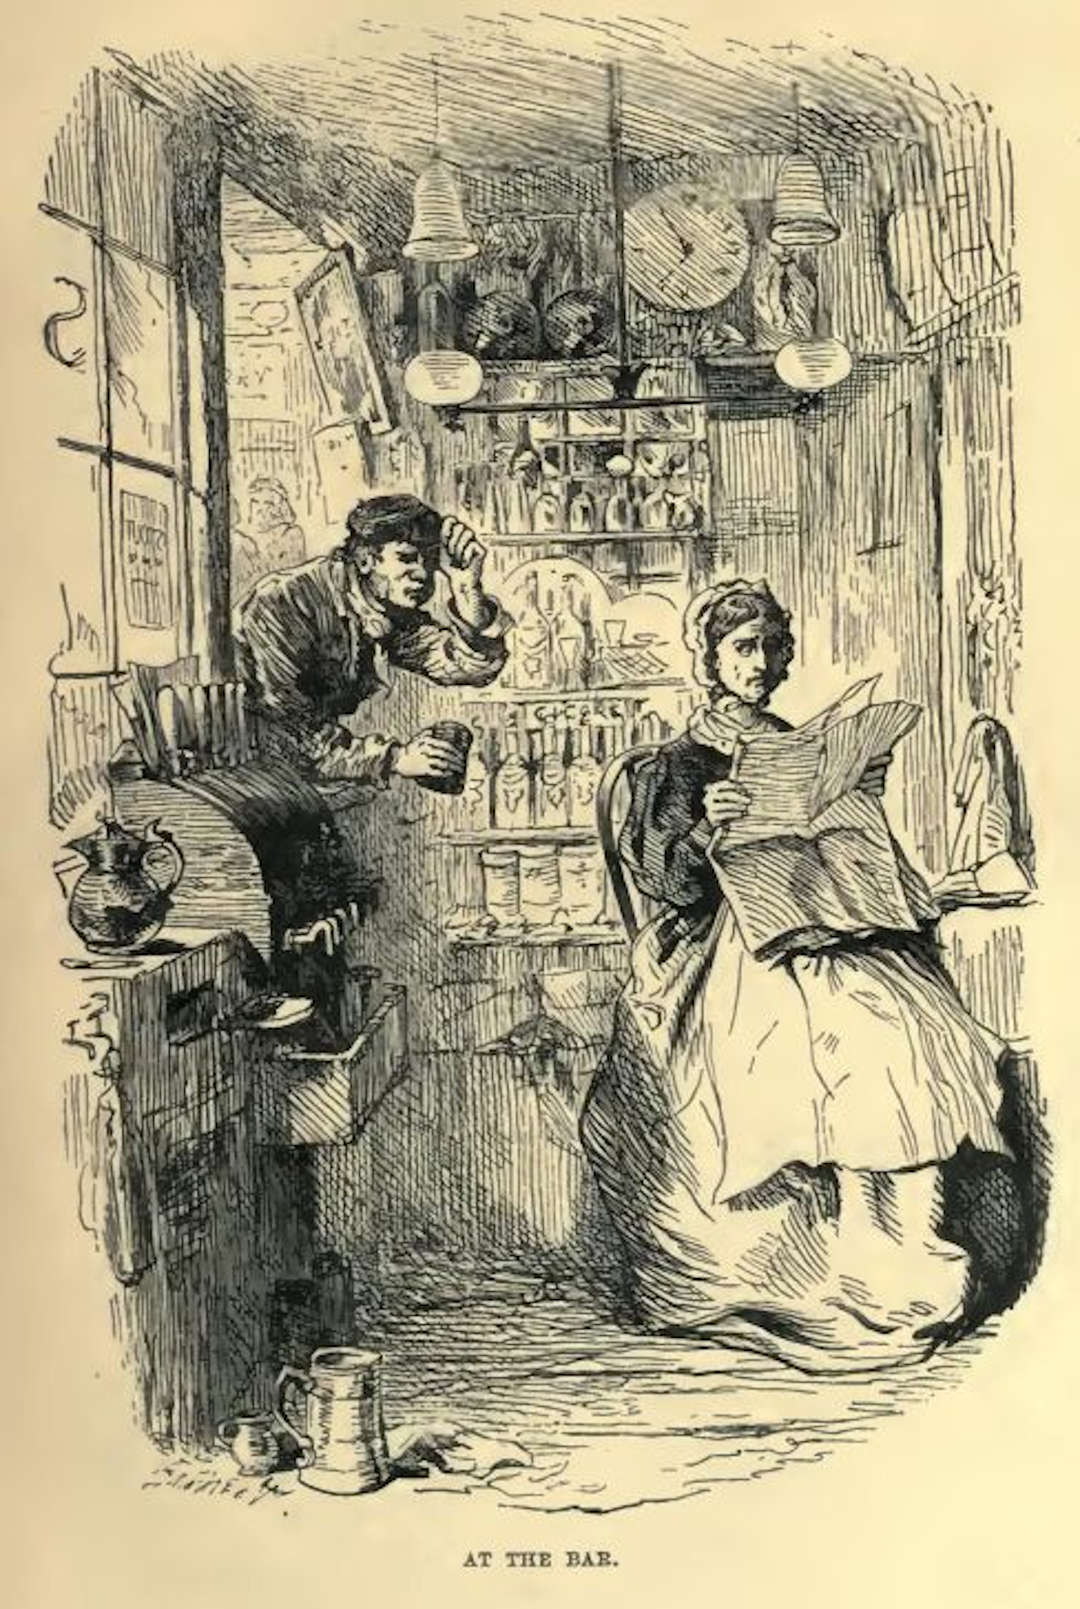
\includegraphics[scale=2.3]{01-06-01}

Chapter 8

MR BOFFIN IN CONSULTATION


Whosoever had gone out of Fleet Street into the Temple at the date of
this history, and had wandered disconsolate about the Temple until he
stumbled on a dismal churchyard, and had looked up at the dismal windows
commanding that churchyard until at the most dismal window of them
all he saw a dismal boy, would in him have beheld, at one grand
comprehensive swoop of the eye, the managing clerk, junior clerk,
common-law clerk, conveyancing clerk, chancery clerk, every refinement
and department of clerk, of Mr Mortimer Lightwood, erewhile called in
the newspapers eminent solicitor.

Mr Boffin having been several times in communication with this clerkly
essence, both on its own ground and at the Bower, had no difficulty in
identifying it when he saw it up in its dusty eyrie. To the second floor
on which the window was situated, he ascended, much pre-occupied in mind
by the uncertainties besetting the Roman Empire, and much regretting the
death of the amiable Pertinax: who only last night had left the Imperial
affairs in a state of great confusion, by falling a victim to the fury
of the praetorian guards.

‘Morning, morning, morning!’ said Mr Boffin, with a wave of his hand, as
the office door was opened by the dismal boy, whose appropriate name was
Blight. ‘Governor in?’

‘Mr Lightwood gave you an appointment, sir, I think?’

‘I don’t want him to give it, you know,’ returned Mr Boffin; ‘I’ll pay
my way, my boy.’

‘No doubt, sir. Would you walk in? Mr Lightwood ain’t in at the present
moment, but I expect him back very shortly. Would you take a seat in Mr
Lightwood’s room, sir, while I look over our Appointment Book?’
Young Blight made a great show of fetching from his desk a long thin
manuscript volume with a brown paper cover, and running his finger down
the day’s appointments, murmuring, ‘Mr Aggs, Mr Baggs, Mr Caggs, Mr
Daggs, Mr Faggs, Mr Gaggs, Mr Boffin. Yes, sir; quite right. You are a
little before your time, sir. Mr Lightwood will be in directly.’

‘I’m not in a hurry,’ said Mr Boffin

‘Thank you, sir. I’ll take the opportunity, if you please, of entering
your name in our Callers’ Book for the day.’ Young Blight made another
great show of changing the volume, taking up a pen, sucking it, dipping
it, and running over previous entries before he wrote. As, ‘Mr Alley,
Mr Balley, Mr Calley, Mr Dalley, Mr Falley, Mr Galley, Mr Halley, Mr
Lalley, Mr Malley. And Mr Boffin.’

‘Strict system here; eh, my lad?’ said Mr Boffin, as he was booked.

‘Yes, sir,’ returned the boy. ‘I couldn’t get on without it.’

By which he probably meant that his mind would have been shattered to
pieces without this fiction of an occupation. Wearing in his solitary
confinement no fetters that he could polish, and being provided with no
drinking-cup that he could carve, he had fallen on the device of ringing
alphabetical changes into the two volumes in question, or of entering
vast numbers of persons out of the Directory as transacting business
with Mr Lightwood. It was the more necessary for his spirits, because,
being of a sensitive temperament, he was apt to consider it personally
disgraceful to himself that his master had no clients.

‘How long have you been in the law, now?’ asked Mr Boffin, with a
pounce, in his usual inquisitive way.

‘I’ve been in the law, now, sir, about three years.’

‘Must have been as good as born in it!’ said Mr Boffin, with admiration.
‘Do you like it?’

‘I don’t mind it much,’ returned Young Blight, heaving a sigh, as if its
bitterness were past.

‘What wages do you get?’

‘Half what I could wish,’ replied young Blight.

‘What’s the whole that you could wish?’

‘Fifteen shillings a week,’ said the boy.

‘About how long might it take you now, at a average rate of going, to be
a Judge?’ asked Mr Boffin, after surveying his small stature in silence.

The boy answered that he had not yet quite worked out that little
calculation.

‘I suppose there’s nothing to prevent your going in for it?’ said Mr
Boffin.

The boy virtually replied that as he had the honour to be a Briton who
never never never, there was nothing to prevent his going in for it. Yet
he seemed inclined to suspect that there might be something to prevent
his coming out with it.

‘Would a couple of pound help you up at all?’ asked Mr Boffin.

On this head, young Blight had no doubt whatever, so Mr Boffin made him
a present of that sum of money, and thanked him for his attention to his
(Mr Boffin’s) affairs; which, he added, were now, he believed, as good
as settled.

Then Mr Boffin, with his stick at his ear, like a Familiar Spirit
explaining the office to him, sat staring at a little bookcase of Law
Practice and Law Reports, and at a window, and at an empty blue bag, and
at a stick of sealing-wax, and a pen, and a box of wafers, and an apple,
and a writing-pad--all very dusty--and at a number of inky smears
and blots, and at an imperfectly-disguised gun-case pretending to be
something legal, and at an iron box labelled HARMON ESTATE, until Mr
Lightwood appeared.

Mr Lightwood explained that he came from the proctor’s, with whom he had
been engaged in transacting Mr Boffin’s affairs.

‘And they seem to have taken a deal out of you!’ said Mr Boffin, with
commiseration.

Mr Lightwood, without explaining that his weariness was chronic,
proceeded with his exposition that, all forms of law having been at
length complied with, will of Harmon deceased having been proved, death
of Harmon next inheriting having been proved, \&{c}., and so forth, Court
of Chancery having been moved, \&{c}. and so forth, he, Mr Lightwood, had
now the gratification, honour, and happiness, again \&{c}. and so forth, of
congratulating Mr Boffin on coming into possession as residuary legatee,
of upwards of one hundred thousand pounds, standing in the books of the
Governor and Company of the Bank of England, again \&{c}. and so forth.

‘And what is particularly eligible in the property Mr Boffin, is, that
it involves no trouble. There are no estates to manage, no rents to
return so much per cent upon in bad times (which is an extremely dear
way of getting your name into the newspapers), no voters to become
parboiled in hot water with, no agents to take the cream off the
milk before it comes to table. You could put the whole in a cash-box
to-morrow morning, and take it with you to--say, to the Rocky Mountains.
Inasmuch as every man,’ concluded Mr Lightwood, with an indolent smile,
‘appears to be under a fatal spell which obliges him, sooner or later,
to mention the Rocky Mountains in a tone of extreme familiarity to some
other man, I hope you’ll excuse my pressing you into the service of that
gigantic range of geographical bores.’

Without following this last remark very closely, Mr Boffin cast his
perplexed gaze first at the ceiling, and then at the carpet.

‘Well,’ he remarked, ‘I don’t know what to say about it, I am sure. I
was a’most as well as I was. It’s a great lot to take care of.’

‘My dear Mr Boffin, then DON’T take care of it!’

‘Eh?’ said that gentleman.

‘Speaking now,’ returned Mortimer, ‘with the irresponsible imbecility
of a private individual, and not with the profundity of a professional
adviser, I should say that if the circumstance of its being too much,
weighs upon your mind, you have the haven of consolation open to you
that you can easily make it less. And if you should be apprehensive of
the trouble of doing so, there is the further haven of consolation that
any number of people will take the trouble off your hands.’

‘Well! I don’t quite see it,’ retorted Mr Boffin, still perplexed.
‘That’s not satisfactory, you know, what you’re a-saying.’

‘Is Anything satisfactory, Mr Boffin?’ asked Mortimer, raising his
eyebrows.

‘I used to find it so,’ answered Mr Boffin, with a wistful look. ‘While
I was foreman at the Bower--afore it WAS the Bower--I considered the
business very satisfactory. The old man was a awful Tartar (saying
it, I’m sure, without disrespect to his memory) but the business was
a pleasant one to look after, from before daylight to past dark. It’s
a’most a pity,’ said Mr Boffin, rubbing his ear, ‘that he ever went and
made so much money. It would have been better for him if he hadn’t so
given himself up to it. You may depend upon it,’ making the discovery
all of a sudden, ‘that HE found it a great lot to take care of!’

Mr Lightwood coughed, not convinced.

‘And speaking of satisfactory,’ pursued Mr Boffin, ‘why, Lord save
us! when we come to take it to pieces, bit by bit, where’s the
satisfactoriness of the money as yet? When the old man does right the
poor boy after all, the poor boy gets no good of it. He gets made away
with, at the moment when he’s lifting (as one may say) the cup and
sarser to his lips. Mr Lightwood, I will now name to you, that on behalf
of the poor dear boy, me and Mrs Boffin have stood out against the old
man times out of number, till he has called us every name he could lay
his tongue to. I have seen him, after Mrs Boffin has given him her mind
respecting the claims of the nat’ral affections, catch off Mrs Boffin’s
bonnet (she wore, in general, a black straw, perched as a matter of
convenience on the top of her head), and send it spinning across
the yard. I have indeed. And once, when he did this in a manner that
amounted to personal, I should have given him a rattler for himself, if
Mrs Boffin hadn’t thrown herself betwixt us, and received flush on the
temple. Which dropped her, Mr Lightwood. Dropped her.’

Mr Lightwood murmured ‘Equal honour--Mrs Boffin’s head and heart.’

‘You understand; I name this,’ pursued Mr Boffin, ‘to show you, now the
affairs are wound up, that me and Mrs Boffin have ever stood as we were
in Christian honour bound, the children’s friend. Me and Mrs Boffin
stood the poor girl’s friend; me and Mrs Boffin stood the poor boy’s
friend; me and Mrs Boffin up and faced the old man when we momently
expected to be turned out for our pains. As to Mrs Boffin,’ said Mr
Boffin lowering his voice, ‘she mightn’t wish it mentioned now she’s
Fashionable, but she went so far as to tell him, in my presence, he was
a flinty-hearted rascal.’

Mr Lightwood murmured ‘Vigorous Saxon spirit--Mrs Boffin’s
ancestors--bowmen--Agincourt and Cressy.’

‘The last time me and Mrs Boffin saw the poor boy,’ said Mr Boffin,
warming (as fat usually does) with a tendency to melt, ‘he was a child
of seven year old. For when he came back to make intercession for his
sister, me and Mrs Boffin were away overlooking a country contract which
was to be sifted before carted, and he was come and gone in a single
hour. I say he was a child of seven year old. He was going away, all
alone and forlorn, to that foreign school, and he come into our place,
situate up the yard of the present Bower, to have a warm at our fire.
There was his little scanty travelling clothes upon him. There was his
little scanty box outside in the shivering wind, which I was going to
carry for him down to the steamboat, as the old man wouldn’t hear of
allowing a sixpence coach-money. Mrs Boffin, then quite a young woman
and pictur of a full-blown rose, stands him by her, kneels down at the
fire, warms her two open hands, and falls to rubbing his cheeks; but
seeing the tears come into the child’s eyes, the tears come fast into
her own, and she holds him round the neck, like as if she was protecting
him, and cries to me, “I’d give the wide wide world, I would, to run
away with him!” I don’t say but what it cut me, and but what it at the
same time heightened my feelings of admiration for Mrs Boffin. The poor
child clings to her for awhile, as she clings to him, and then, when
the old man calls, he says “I must go! God bless you!” and for a moment
rests his heart against her bosom, and looks up at both of us, as if it
was in pain--in agony. Such a look! I went aboard with him (I gave him
first what little treat I thought he’d like), and I left him when he had
fallen asleep in his berth, and I came back to Mrs Boffin. But tell
her what I would of how I had left him, it all went for nothing, for,
according to her thoughts, he never changed that look that he had looked
up at us two. But it did one piece of good. Mrs Boffin and me had no
child of our own, and had sometimes wished that how we had one. But not
now. “We might both of us die,” says Mrs Boffin, “and other eyes might
see that lonely look in our child.” So of a night, when it was very
cold, or when the wind roared, or the rain dripped heavy, she would
wake sobbing, and call out in a fluster, “Don’t you see the poor child’s
face? O shelter the poor child!”--till in course of years it gently wore
out, as many things do.’

‘My dear Mr Boffin, everything wears to rags,’ said Mortimer, with a
light laugh.

‘I won’t go so far as to say everything,’ returned Mr Boffin, on whom
his manner seemed to grate, ‘because there’s some things that I never
found among the dust. Well, sir. So Mrs Boffin and me grow older and
older in the old man’s service, living and working pretty hard in it,
till the old man is discovered dead in his bed. Then Mrs Boffin and me
seal up his box, always standing on the table at the side of his bed,
and having frequently heerd tell of the Temple as a spot where lawyer’s
dust is contracted for, I come down here in search of a lawyer to
advise, and I see your young man up at this present elevation, chopping
at the flies on the window-sill with his penknife, and I give him a Hoy!
not then having the pleasure of your acquaintance, and by that
means come to gain the honour. Then you, and the gentleman in the
uncomfortable neck-cloth under the little archway in Saint Paul’s
Churchyard--’

‘Doctors’ Commons,’ observed Lightwood.

‘I understood it was another name,’ said Mr Boffin, pausing, ‘but you
know best. Then you and Doctor Scommons, you go to work, and you do the
thing that’s proper, and you and Doctor S. take steps for finding out
the poor boy, and at last you do find out the poor boy, and me and Mrs
Boffin often exchange the observation, “We shall see him again,
under happy circumstances.” But it was never to be; and the want of
satisfactoriness is, that after all the money never gets to him.’

‘But it gets,’ remarked Lightwood, with a languid inclination of the
head, ‘into excellent hands.’

‘It gets into the hands of me and Mrs Boffin only this very day and
hour, and that’s what I am working round to, having waited for this day
and hour a’ purpose. Mr Lightwood, here has been a wicked cruel
murder. By that murder me and Mrs Boffin mysteriously profit. For the
apprehension and conviction of the murderer, we offer a reward of one
tithe of the property--a reward of Ten Thousand Pound.’

‘Mr Boffin, it’s too much.’

‘Mr Lightwood, me and Mrs Boffin have fixed the sum together, and we
stand to it.’

‘But let me represent to you,’ returned Lightwood, ‘speaking now with
professional profundity, and not with individual imbecility, that the
offer of such an immense reward is a temptation to forced suspicion,
forced construction of circumstances, strained accusation, a whole
tool-box of edged tools.’

‘Well,’ said Mr Boffin, a little staggered, ‘that’s the sum we put o’
one side for the purpose. Whether it shall be openly declared in the new
notices that must now be put about in our names--’

‘In your name, Mr Boffin; in your name.’

‘Very well; in my name, which is the same as Mrs Boffin’s, and means
both of us, is to be considered in drawing ‘em up. But this is the first
instruction that I, as the owner of the property, give to my lawyer on
coming into it.’

‘Your lawyer, Mr Boffin,’ returned Lightwood, making a very short
note of it with a very rusty pen, ‘has the gratification of taking the
instruction. There is another?’

‘There is just one other, and no more. Make me as compact a little will
as can be reconciled with tightness, leaving the whole of the property
to “my beloved wife, Henerietty Boffin, sole executrix”. Make it as
short as you can, using those words; but make it tight.’

At some loss to fathom Mr Boffin’s notions of a tight will, Lightwood
felt his way.

‘I beg your pardon, but professional profundity must be exact. When you
say tight--’

‘I mean tight,’ Mr Boffin explained.

‘Exactly so. And nothing can be more laudable. But is the tightness to
bind Mrs Boffin to any and what conditions?’

‘Bind Mrs Boffin?’ interposed her husband. ‘No! What are you thinking
of! What I want is, to make it all hers so tight as that her hold of it
can’t be loosed.’

‘Hers freely, to do what she likes with? Hers absolutely?’

‘Absolutely?’ repeated Mr Boffin, with a short sturdy laugh. ‘Hah! I
should think so! It would be handsome in me to begin to bind Mrs Boffin
at this time of day!’

So that instruction, too, was taken by Mr Lightwood; and Mr Lightwood,
having taken it, was in the act of showing Mr Boffin out, when Mr Eugene
Wrayburn almost jostled him in the door-way. Consequently Mr Lightwood
said, in his cool manner, ‘Let me make you two known to one another,’
and further signified that Mr Wrayburn was counsel learned in the
law, and that, partly in the way of business and partly in the way of
pleasure, he had imparted to Mr Wrayburn some of the interesting facts
of Mr Boffin’s biography.

‘Delighted,’ said Eugene--though he didn’t look so--‘to know Mr Boffin.’

‘Thankee, sir, thankee,’ returned that gentleman. ‘And how do YOU like
the law?’

‘A--not particularly,’ returned Eugene.

‘Too dry for you, eh? Well, I suppose it wants some years of sticking
to, before you master it. But there’s nothing like work. Look at the
bees.’

‘I beg your pardon,’ returned Eugene, with a reluctant smile, ‘but will
you excuse my mentioning that I always protest against being referred to
the bees?’

‘Do you!’ said Mr Boffin.

‘I object on principle,’ said Eugene, ‘as a biped--’

‘As a what?’ asked Mr Boffin.

‘As a two-footed creature;--I object on principle, as a two-footed
creature, to being constantly referred to insects and four-footed
creatures. I object to being required to model my proceedings according
to the proceedings of the bee, or the dog, or the spider, or the camel.
I fully admit that the camel, for instance, is an excessively temperate
person; but he has several stomachs to entertain himself with, and I
have only one. Besides, I am not fitted up with a convenient cool cellar
to keep my drink in.’

‘But I said, you know,’ urged Mr Boffin, rather at a loss for an answer,
‘the bee.’

‘Exactly. And may I represent to you that it’s injudicious to say the
bee? For the whole case is assumed. Conceding for a moment that there is
any analogy between a bee, and a man in a shirt and pantaloons (which
I deny), and that it is settled that the man is to learn from the bee
(which I also deny), the question still remains, what is he to learn?
To imitate? Or to avoid? When your friends the bees worry themselves to
that highly fluttered extent about their sovereign, and become perfectly
distracted touching the slightest monarchical movement, are we men to
learn the greatness of Tuft-hunting, or the littleness of the
Court Circular? I am not clear, Mr Boffin, but that the hive may be
satirical.’

‘At all events, they work,’ said Mr Boffin.

‘Ye-es,’ returned Eugene, disparagingly, ‘they work; but don’t you think
they overdo it? They work so much more than they need--they make so much
more than they can eat--they are so incessantly boring and buzzing at
their one idea till Death comes upon them--that don’t you think they
overdo it? And are human labourers to have no holidays, because of the
bees? And am I never to have change of air, because the bees don’t? Mr
Boffin, I think honey excellent at breakfast; but, regarded in the light
of my conventional schoolmaster and moralist, I protest against the
tyrannical humbug of your friend the bee. With the highest respect for
you.’

‘Thankee,’ said Mr Boffin. ‘Morning, morning!’

But, the worthy Mr Boffin jogged away with a comfortless impression he
could have dispensed with, that there was a deal of unsatisfactoriness
in the world, besides what he had recalled as appertaining to the Harmon
property. And he was still jogging along Fleet Street in this condition
of mind, when he became aware that he was closely tracked and observed
by a man of genteel appearance.

‘Now then?’ said Mr Boffin, stopping short, with his meditations brought
to an abrupt check, ‘what’s the next article?’

‘I beg your pardon, Mr Boffin.’

‘My name too, eh? How did you come by it? I don’t know you.’

‘No, sir, you don’t know me.’

Mr Boffin looked full at the man, and the man looked full at him.

‘No,’ said Mr Boffin, after a glance at the pavement, as if it were made
of faces and he were trying to match the man’s, ‘I DON’T know you.’

‘I am nobody,’ said the stranger, ‘and not likely to be known; but Mr
Boffin’s wealth--’

‘Oh! that’s got about already, has it?’ muttered Mr Boffin.

‘--And his romantic manner of acquiring it, make him conspicuous. You
were pointed out to me the other day.’

‘Well,’ said Mr Boffin, ‘I should say I was a disappintment to you when
I WAS pinted out, if your politeness would allow you to confess it, for
I am well aware I am not much to look at. What might you want with me?
Not in the law, are you?’

‘No, sir.’

‘No information to give, for a reward?’

‘No, sir.’

There may have been a momentary mantling in the face of the man as he
made the last answer, but it passed directly.

‘If I don’t mistake, you have followed me from my lawyer’s and tried
to fix my attention. Say out! Have you? Or haven’t you?’ demanded Mr
Boffin, rather angry.

‘Yes.’

‘Why have you?’

‘If you will allow me to walk beside you, Mr Boffin, I will tell you.
Would you object to turn aside into this place--I think it is called
Clifford’s Inn--where we can hear one another better than in the roaring
street?’

[‘Now,’ thought Mr Boffin, ‘if he proposes a game at skittles, or meets
a country gentleman just come into property, or produces any article
of jewellery he has found, I’ll knock him down!’ With this discreet
reflection, and carrying his stick in his arms much as Punch carries
his, Mr Boffin turned into Clifford’s Inn aforesaid.)

‘Mr Boffin, I happened to be in Chancery Lane this morning, when I saw
you going along before me. I took the liberty of following you, trying
to make up my mind to speak to you, till you went into your lawyer’s.
Then I waited outside till you came out.’

[‘Don’t quite sound like skittles, nor yet country gentleman, nor yet
jewellery,’ thought Mr Boffin, ‘but there’s no knowing.’)

‘I am afraid my object is a bold one, I am afraid it has little of the
usual practical world about it, but I venture it. If you ask me, or if
you ask yourself--which is more likely--what emboldens me, I answer, I
have been strongly assured, that you are a man of rectitude and plain
dealing, with the soundest of sound hearts, and that you are blessed in
a wife distinguished by the same qualities.’

‘Your information is true of Mrs Boffin, anyhow,’ was Mr Boffin’s
answer, as he surveyed his new friend again. There was something
repressed in the strange man’s manner, and he walked with his eyes
on the ground--though conscious, for all that, of Mr Boffin’s
observation--and he spoke in a subdued voice. But his words came easily,
and his voice was agreeable in tone, albeit constrained.

‘When I add, I can discern for myself what the general tongue says of
you--that you are quite unspoiled by Fortune, and not uplifted--I trust
you will not, as a man of an open nature, suspect that I mean to flatter
you, but will believe that all I mean is to excuse myself, these being
my only excuses for my present intrusion.’

[‘How much?’ thought Mr Boffin. ‘It must be coming to money. How much?’)

‘You will probably change your manner of living, Mr Boffin, in your
changed circumstances. You will probably keep a larger house, have many
matters to arrange, and be beset by numbers of correspondents. If you
would try me as your Secretary--’

‘As WHAT?’ cried Mr Boffin, with his eyes wide open.

‘Your Secretary.’

‘Well,’ said Mr Boffin, under his breath, ‘that’s a queer thing!’

‘Or,’ pursued the stranger, wondering at Mr Boffin’s wonder, ‘if you
would try me as your man of business under any name, I know you would
find me faithful and grateful, and I hope you would find me useful. You
may naturally think that my immediate object is money. Not so, for
I would willingly serve you a year--two years--any term you might
appoint--before that should begin to be a consideration between us.’

‘Where do you come from?’ asked Mr Boffin.

‘I come,’ returned the other, meeting his eye, ‘from many countries.’

Boffin’s acquaintances with the names and situations of foreign lands
being limited in extent and somewhat confused in quality, he shaped his
next question on an elastic model.

‘From--any particular place?’

‘I have been in many places.’

‘What have you been?’ asked Mr Boffin.

Here again he made no great advance, for the reply was, ‘I have been a
student and a traveller.’

‘But if it ain’t a liberty to plump it out,’ said Mr Boffin, ‘what do
you do for your living?’

‘I have mentioned,’ returned the other, with another look at him, and
a smile, ‘what I aspire to do. I have been superseded as to some slight
intentions I had, and I may say that I have now to begin life.’

Not very well knowing how to get rid of this applicant, and feeling the
more embarrassed because his manner and appearance claimed a delicacy
in which the worthy Mr Boffin feared he himself might be deficient, that
gentleman glanced into the mouldy little plantation or cat-preserve, of
Clifford’s Inn, as it was that day, in search of a suggestion. Sparrows
were there, cats were there, dry-rot and wet-rot were there, but it was
not otherwise a suggestive spot.

‘All this time,’ said the stranger, producing a little pocket-book and
taking out a card, ‘I have not mentioned my name. My name is Rokesmith.
I lodge at one Mr Wilfer’s, at Holloway.’

Mr Boffin stared again.

‘Father of Miss Bella Wilfer?’ said he.

‘My landlord has a daughter named Bella. Yes; no doubt.’

Now, this name had been more or less in Mr Boffin’s thoughts all the
morning, and for days before; therefore he said:

‘That’s singular, too!’ unconsciously staring again, past all bounds of
good manners, with the card in his hand. ‘Though, by-the-bye, I suppose
it was one of that family that pinted me out?’

‘No. I have never been in the streets with one of them.’

‘Heard me talked of among ‘em, though?’

‘No. I occupy my own rooms, and have held scarcely any communication
with them.’

‘Odder and odder!’ said Mr Boffin. ‘Well, sir, to tell you the truth, I
don’t know what to say to you.’

‘Say nothing,’ returned Mr Rokesmith; ‘allow me to call on you in a few
days. I am not so unconscionable as to think it likely that you would
accept me on trust at first sight, and take me out of the very street.
Let me come to you for your further opinion, at your leisure.’

‘That’s fair, and I don’t object,’ said Mr Boffin; ‘but it must be on
condition that it’s fully understood that I no more know that I shall
ever be in want of any gentleman as Secretary--it WAS Secretary you
said; wasn’t it?’

‘Yes.’

Again Mr Boffin’s eyes opened wide, and he stared at the applicant from
head to foot, repeating ‘Queer!--You’re sure it was Secretary? Are you?’

‘I am sure I said so.’

--‘As Secretary,’ repeated Mr Boffin, meditating upon the word; ‘I no
more know that I may ever want a Secretary, or what not, than I do that
I shall ever be in want of the man in the moon. Me and Mrs Boffin have
not even settled that we shall make any change in our way of life. Mrs
Boffin’s inclinations certainly do tend towards Fashion; but, being
already set up in a fashionable way at the Bower, she may not make
further alterations. However, sir, as you don’t press yourself, I wish
to meet you so far as saying, by all means call at the Bower if you
like. Call in the course of a week or two. At the same time, I consider
that I ought to name, in addition to what I have already named, that I
have in my employment a literary man--WITH a wooden leg--as I have no
thoughts of parting from.’

‘I regret to hear I am in some sort anticipated,’ Mr Rokesmith answered,
evidently having heard it with surprise; ‘but perhaps other duties might
arise?’

‘You see,’ returned Mr Boffin, with a confidential sense of dignity, ‘as
to my literary man’s duties, they’re clear. Professionally he declines
and he falls, and as a friend he drops into poetry.’

Without observing that these duties seemed by no means clear to Mr
Rokesmith’s astonished comprehension, Mr Boffin went on:

‘And now, sir, I’ll wish you good-day. You can call at the Bower any
time in a week or two. It’s not above a mile or so from you, and your
landlord can direct you to it. But as he may not know it by its new
name of Boffin’s Bower, say, when you inquire of him, it’s Harmon’s;
will you?’

‘Harmoon’s,’ repeated Mr Rokesmith, seeming to have caught the sound
imperfectly, ‘Harmarn’s. How do you spell it?’

‘Why, as to the spelling of it,’ returned Mr Boffin, with great presence
of mind, ‘that’s YOUR look out. Harmon’s is all you’ve got to say to
HIM. Morning, morning, morning!’ And so departed, without looking back.



Chapter 9

MR AND MRS BOFFIN IN CONSULTATION


Betaking himself straight homeward, Mr Boffin, without further let or
hindrance, arrived at the Bower, and gave Mrs Boffin (in a walking dress
of black velvet and feathers, like a mourning coach-horse) an account of
all he had said and done since breakfast.

‘This brings us round, my dear,’ he then pursued, ‘to the question
we left unfinished: namely, whether there’s to be any new go-in for
Fashion.’

‘Now, I’ll tell you what I want, Noddy,’ said Mrs Boffin, smoothing her
dress with an air of immense enjoyment, ‘I want Society.’

‘Fashionable Society, my dear?’

‘Yes!’ cried Mrs Boffin, laughing with the glee of a child. ‘Yes! It’s
no good my being kept here like Wax-Work; is it now?’

‘People have to pay to see Wax-Work, my dear,’ returned her husband,
‘whereas (though you’d be cheap at the same money) the neighbours is
welcome to see YOU for nothing.’

‘But it don’t answer,’ said the cheerful Mrs Boffin. ‘When we worked
like the neighbours, we suited one another. Now we have left work off;
we have left off suiting one another.’

‘What, do you think of beginning work again?’ Mr Boffin hinted.

‘Out of the question! We have come into a great fortune, and we must do
what’s right by our fortune; we must act up to it.’

Mr Boffin, who had a deep respect for his wife’s intuitive wisdom,
replied, though rather pensively: ‘I suppose we must.’

‘It’s never been acted up to yet, and, consequently, no good has come of
it,’ said Mrs Boffin.

‘True, to the present time,’ Mr Boffin assented, with his former
pensiveness, as he took his seat upon his settle. ‘I hope good may be
coming of it in the future time. Towards which, what’s your views, old
lady?’

Mrs Boffin, a smiling creature, broad of figure and simple of nature,
with her hands folded in her lap, and with buxom creases in her throat,
proceeded to expound her views.

‘I say, a good house in a good neighbourhood, good things about us,
good living, and good society. I say, live like our means, without
extravagance, and be happy.’

‘Yes. I say be happy, too,’ assented the still pensive Mr Boffin.
‘Lor-a-mussy!’ exclaimed Mrs Boffin, laughing and clapping her hands,
and gaily rocking herself to and fro, ‘when I think of me in a light
yellow chariot and pair, with silver boxes to the wheels--’

‘Oh! you was thinking of that, was you, my dear?’

‘Yes!’ cried the delighted creature. ‘And with a footman up behind, with
a bar across, to keep his legs from being poled! And with a coachman
up in front, sinking down into a seat big enough for three of him, all
covered with upholstery in green and white! And with two bay horses
tossing their heads and stepping higher than they trot long-ways! And
with you and me leaning back inside, as grand as ninepence! Oh-h-h-h My!
Ha ha ha ha ha!’

Mrs Boffin clapped her hands again, rocked herself again, beat her feet
upon the floor, and wiped the tears of laughter from her eyes.

‘And what, my old lady,’ inquired Mr Boffin, when he also had
sympathetically laughed: ‘what’s your views on the subject of the
Bower?’

‘Shut it up. Don’t part with it, but put somebody in it, to keep it.’

‘Any other views?’

‘Noddy,’ said Mrs Boffin, coming from her fashionable sofa to his side
on the plain settle, and hooking her comfortable arm through his,
‘Next I think--and I really have been thinking early and late--of the
disappointed girl; her that was so cruelly disappointed, you know, both
of her husband and his riches. Don’t you think we might do something for
her? Have her to live with us? Or something of that sort?’

‘Ne-ver once thought of the way of doing it!’ cried Mr Boffin, smiting
the table in his admiration. ‘What a thinking steam-ingein this old lady
is. And she don’t know how she does it. Neither does the ingein!’

Mrs Boffin pulled his nearest ear, in acknowledgment of this piece of
philosophy, and then said, gradually toning down to a motherly strain:
‘Last, and not least, I have taken a fancy. You remember dear little
John Harmon, before he went to school? Over yonder across the yard, at
our fire? Now that he is past all benefit of the money, and it’s come to
us, I should like to find some orphan child, and take the boy and adopt
him and give him John’s name, and provide for him. Somehow, it would
make me easier, I fancy. Say it’s only a whim--’

‘But I don’t say so,’ interposed her husband.

‘No, but deary, if you did--’

‘I should be a Beast if I did,’ her husband interposed again.

‘That’s as much as to say you agree? Good and kind of you, and like you,
deary! And don’t you begin to find it pleasant now,’ said Mrs Boffin,
once more radiant in her comely way from head to foot, and once more
smoothing her dress with immense enjoyment, ‘don’t you begin to find
it pleasant already, to think that a child will be made brighter, and
better, and happier, because of that poor sad child that day? And isn’t
it pleasant to know that the good will be done with the poor sad child’s
own money?’

‘Yes; and it’s pleasant to know that you are Mrs Boffin,’ said her
husband, ‘and it’s been a pleasant thing to know this many and many a
year!’ It was ruin to Mrs Boffin’s aspirations, but, having so spoken,
they sat side by side, a hopelessly Unfashionable pair.

These two ignorant and unpolished people had guided themselves so far on
in their journey of life, by a religious sense of duty and desire to do
right. Ten thousand weaknesses and absurdities might have been detected
in the breasts of both; ten thousand vanities additional, possibly, in
the breast of the woman. But the hard wrathful and sordid nature that
had wrung as much work out of them as could be got in their best days,
for as little money as could be paid to hurry on their worst, had never
been so warped but that it knew their moral straightness and respected
it. In its own despite, in a constant conflict with itself and them, it
had done so. And this is the eternal law. For, Evil often stops short at
itself and dies with the doer of it; but Good, never.

Through his most inveterate purposes, the dead Jailer of Harmony Jail
had known these two faithful servants to be honest and true. While he
raged at them and reviled them for opposing him with the speech of the
honest and true, it had scratched his stony heart, and he had perceived
the powerlessness of all his wealth to buy them if he had addressed
himself to the attempt. So, even while he was their griping taskmaster
and never gave them a good word, he had written their names down in his
will. So, even while it was his daily declaration that he mistrusted all
mankind--and sorely indeed he did mistrust all who bore any resemblance
to himself--he was as certain that these two people, surviving him,
would be trustworthy in all things from the greatest to the least, as he
was that he must surely die.

Mr and Mrs Boffin, sitting side by side, with Fashion withdrawn to an
immeasurable distance, fell to discussing how they could best find their
orphan. Mrs Boffin suggested advertisement in the newspapers, requesting
orphans answering annexed description to apply at the Bower on a certain
day; but Mr Boffin wisely apprehending obstruction of the neighbouring
thoroughfares by orphan swarms, this course was negatived. Mrs Boffin
next suggested application to their clergyman for a likely orphan. Mr
Boffin thinking better of this scheme, they resolved to call upon the
reverend gentleman at once, and to take the same opportunity of making
acquaintance with Miss Bella Wilfer. In order that these visits might be
visits of state, Mrs Boffin’s equipage was ordered out.

This consisted of a long hammer-headed old horse, formerly used in the
business, attached to a four-wheeled chaise of the same period, which
had long been exclusively used by the Harmony Jail poultry as the
favourite laying-place of several discreet hens. An unwonted application
of corn to the horse, and of paint and varnish to the carriage, when
both fell in as a part of the Boffin legacy, had made what Mr Boffin
considered a neat turn-out of the whole; and a driver being added, in
the person of a long hammer-headed young man who was a very good match
for the horse, left nothing to be desired. He, too, had been formerly
used in the business, but was now entombed by an honest jobbing tailor
of the district in a perfect Sepulchre of coat and gaiters, sealed with
ponderous buttons.

Behind this domestic, Mr and Mrs Boffin took their seats in the back
compartment of the vehicle: which was sufficiently commodious, but had
an undignified and alarming tendency, in getting over a rough crossing,
to hiccup itself away from the front compartment. On their being
descried emerging from the gates of the Bower, the neighbourhood turned
out at door and window to salute the Boffins. Among those who were ever
and again left behind, staring after the equipage, were many youthful
spirits, who hailed it in stentorian tones with such congratulations as
‘Nod-dy Bof-fin!’ ‘Bof-fin’s mon-ey!’ ‘Down with the dust, Bof-fin!’ and
other similar compliments. These, the hammer-headed young man took in
such ill part that he often impaired the majesty of the progress by
pulling up short, and making as though he would alight to exterminate
the offenders; a purpose from which he only allowed himself to be
dissuaded after long and lively arguments with his employers.

At length the Bower district was left behind, and the peaceful dwelling
of the Reverend Frank Milvey was gained. The Reverend Frank Milvey’s
abode was a very modest abode, because his income was a very modest
income. He was officially accessible to every blundering old woman who
had incoherence to bestow upon him, and readily received the Boffins.
He was quite a young man, expensively educated and wretchedly paid, with
quite a young wife and half a dozen quite young children. He was under
the necessity of teaching and translating from the classics, to eke out
his scanty means, yet was generally expected to have more time to spare
than the idlest person in the parish, and more money than the richest.
He accepted the needless inequalities and inconsistencies of his life,
with a kind of conventional submission that was almost slavish; and any
daring layman who would have adjusted such burdens as his, more decently
and graciously, would have had small help from him.

With a ready patient face and manner, and yet with a latent smile that
showed a quick enough observation of Mrs Boffin’s dress, Mr Milvey, in
his little book-room--charged with sounds and cries as though the six
children above were coming down through the ceiling, and the roasting
leg of mutton below were coming up through the floor--listened to Mrs
Boffin’s statement of her want of an orphan.

‘I think,’ said Mr Milvey, ‘that you have never had a child of your own,
Mr and Mrs Boffin?’

Never.

‘But, like the Kings and Queens in the Fairy Tales, I suppose you have
wished for one?’

In a general way, yes.

Mr Milvey smiled again, as he remarked to himself ‘Those kings and
queens were always wishing for children.’ It occurring to him, perhaps,
that if they had been Curates, their wishes might have tended in the
opposite direction.

‘I think,’ he pursued, ‘we had better take Mrs Milvey into our Council.
She is indispensable to me. If you please, I’ll call her.’

So, Mr Milvey called, ‘Margaretta, my dear!’ and Mrs Milvey came down.
A pretty, bright little woman, something worn by anxiety, who had
repressed many pretty tastes and bright fancies, and substituted in
their stead, schools, soup, flannel, coals, and all the week-day cares
and Sunday coughs of a large population, young and old. As gallantly had
Mr Milvey repressed much in himself that naturally belonged to his old
studies and old fellow-students, and taken up among the poor and their
children with the hard crumbs of life.

‘Mr and Mrs Boffin, my dear, whose good fortune you have heard of.’

Mrs Milvey, with the most unaffected grace in the world, congratulated
them, and was glad to see them. Yet her engaging face, being an open as
well as a perceptive one, was not without her husband’s latent smile.

‘Mrs Boffin wishes to adopt a little boy, my dear.’

Mrs Milvey, looking rather alarmed, her husband added:

‘An orphan, my dear.’

‘Oh!’ said Mrs Milvey, reassured for her own little boys.

‘And I was thinking, Margaretta, that perhaps old Mrs Goody’s grandchild
might answer the purpose.

‘Oh my DEAR Frank! I DON’T think that would do!’

‘No?’

‘Oh NO!’

The smiling Mrs Boffin, feeling it incumbent on her to take part in the
conversation, and being charmed with the emphatic little wife and her
ready interest, here offered her acknowledgments and inquired what there
was against him?

‘I DON’T think,’ said Mrs Milvey, glancing at the Reverend Frank, ‘--and
I believe my husband will agree with me when he considers it again--that
you could possibly keep that orphan clean from snuff. Because his
grandmother takes so MANY ounces, and drops it over him.’

‘But he would not be living with his grandmother then, Margaretta,’ said
Mr Milvey.

‘No, Frank, but it would be impossible to keep her from Mrs Boffin’s
house; and the MORE there was to eat and drink there, the oftener she
would go. And she IS an inconvenient woman. I HOPE it’s not uncharitable
to remember that last Christmas Eve she drank eleven cups of tea, and
grumbled all the time. And she is NOT a grateful woman, Frank. You
recollect her addressing a crowd outside this house, about her wrongs,
when, one night after we had gone to bed, she brought back the petticoat
of new flannel that had been given her, because it was too short.’

‘That’s true,’ said Mr Milvey. ‘I don’t think that would do. Would
little Harrison--’

‘Oh, FRANK!’ remonstrated his emphatic wife.

‘He has no grandmother, my dear.’

‘No, but I DON’T think Mrs Boffin would like an orphan who squints so
MUCH.’

‘That’s true again,’ said Mr Milvey, becoming haggard with perplexity.
‘If a little girl would do--’

‘But, my DEAR Frank, Mrs Boffin wants a boy.’

‘That’s true again,’ said Mr Milvey. ‘Tom Bocker is a nice boy’
(thoughtfully).

‘But I DOUBT, Frank,’ Mrs Milvey hinted, after a little hesitation, ‘if
Mrs Boffin wants an orphan QUITE nineteen, who drives a cart and waters
the roads.’

Mr Milvey referred the point to Mrs Boffin in a look; on that smiling
lady’s shaking her black velvet bonnet and bows, he remarked, in lower
spirits, ‘that’s true again.’

‘I am sure,’ said Mrs Boffin, concerned at giving so much trouble, ‘that
if I had known you would have taken so much pains, sir--and you too, ma’
am--I don’t think I would have come.’

‘PRAY don’t say that!’ urged Mrs Milvey.

‘No, don’t say that,’ assented Mr Milvey, ‘because we are so much
obliged to you for giving us the preference.’ Which Mrs Milvey
confirmed; and really the kind, conscientious couple spoke, as if they
kept some profitable orphan warehouse and were personally patronized.
‘But it is a responsible trust,’ added Mr Milvey, ‘and difficult to
discharge. At the same time, we are naturally very unwilling to lose the
chance you so kindly give us, and if you could afford us a day or two
to look about us,--you know, Margaretta, we might carefully examine the
workhouse, and the Infant School, and your District.’

‘To be SURE!’ said the emphatic little wife.

‘We have orphans, I know,’ pursued Mr Milvey, quite with the air as if
he might have added, ‘in stock,’ and quite as anxiously as if there were
great competition in the business and he were afraid of losing an order,
‘over at the clay-pits; but they are employed by relations or friends,
and I am afraid it would come at last to a transaction in the way of
barter. And even if you exchanged blankets for the child--or books
and firing--it would be impossible to prevent their being turned into
liquor.’

Accordingly, it was resolved that Mr and Mrs Milvey should search for
an orphan likely to suit, and as free as possible from the foregoing
objections, and should communicate again with Mrs Boffin. Then, Mr
Boffin took the liberty of mentioning to Mr Milvey that if Mr Milvey
would do him the kindness to be perpetually his banker to the extent
of ‘a twenty-pound note or so,’ to be expended without any reference
to him, he would be heartily obliged. At this, both Mr Milvey and Mrs
Milvey were quite as much pleased as if they had no wants of their own,
but only knew what poverty was, in the persons of other people; and
so the interview terminated with satisfaction and good opinion on all
sides.

‘Now, old lady,’ said Mr Boffin, as they resumed their seats behind the
hammer-headed horse and man: ‘having made a very agreeable visit there,
we’ll try Wilfer’s.’

It appeared, on their drawing up at the family gate, that to try
Wilfer’s was a thing more easily projected than done, on account of the
extreme difficulty of getting into that establishment; three pulls
at the bell producing no external result; though each was attended
by audible sounds of scampering and rushing within. At the fourth
tug--vindictively administered by the hammer-headed young man--Miss
Lavinia appeared, emerging from the house in an accidental manner, with
a bonnet and parasol, as designing to take a contemplative walk. The
young lady was astonished to find visitors at the gate, and expressed
her feelings in appropriate action.

‘Here’s Mr and Mrs Boffin!’ growled the hammer-headed young man through
the bars of the gate, and at the same time shaking it, as if he were on
view in a Menagerie; ‘they’ve been here half an hour.’

‘Who did you say?’ asked Miss Lavinia.

‘Mr and Mrs BOFFIN’ returned the young man, rising into a roar.

Miss Lavinia tripped up the steps to the house-door, tripped down the
steps with the key, tripped across the little garden, and opened the
gate. ‘Please to walk in,’ said Miss Lavinia, haughtily. ‘Our servant is
out.’

Mr and Mrs Boffin complying, and pausing in the little hall until Miss
Lavinia came up to show them where to go next, perceived three pairs of
listening legs upon the stairs above. Mrs Wilfer’s legs, Miss Bella’s
legs, Mr George Sampson’s legs.

‘Mr and Mrs Boffin, I think?’ said Lavinia, in a warning voice. Strained
attention on the part of Mrs Wilfer’s legs, of Miss Bella’s legs, of Mr
George Sampson’s legs.

‘Yes, Miss.’

‘If you’ll step this way--down these stairs--I’ll let Ma know.’
Excited flight of Mrs Wilfer’s legs, of Miss Bella’s legs, of Mr George
Sampson’s legs.

After waiting some quarter of an hour alone in the family sitting-room,
which presented traces of having been so hastily arranged after a meal,
that one might have doubted whether it was made tidy for visitors,
or cleared for blindman’s buff, Mr and Mrs Boffin became aware of the
entrance of Mrs Wilfer, majestically faint, and with a condescending
stitch in her side: which was her company manner.

‘Pardon me,’ said Mrs Wilfer, after the first salutations, and as soon
as she had adjusted the handkerchief under her chin, and waved her
gloved hands, ‘to what am I indebted for this honour?’

‘To make short of it, ma’am,’ returned Mr Boffin, ‘perhaps you may be
acquainted with the names of me and Mrs Boffin, as having come into a
certain property.’

‘I have heard, sir,’ returned Mrs Wilfer, with a dignified bend of her
head, ‘of such being the case.’

‘And I dare say, ma’am,’ pursued Mr Boffin, while Mrs Boffin added
confirmatory nods and smiles, ‘you are not very much inclined to take
kindly to us?’

‘Pardon me,’ said Mrs Wilfer. ‘’Twere unjust to visit upon Mr and Mrs
Boffin, a calamity which was doubtless a dispensation.’ These words
were rendered the more effective by a serenely heroic expression of
suffering.

‘That’s fairly meant, I am sure,’ remarked the honest Mr Boffin; ‘Mrs
Boffin and me, ma’am, are plain people, and we don’t want to pretend
to anything, nor yet to go round and round at anything because there’s
always a straight way to everything. Consequently, we make this call
to say, that we shall be glad to have the honour and pleasure of your
daughter’s acquaintance, and that we shall be rejoiced if your daughter
will come to consider our house in the light of her home equally with
this. In short, we want to cheer your daughter, and to give her
the opportunity of sharing such pleasures as we are a going to take
ourselves. We want to brisk her up, and brisk her about, and give her a
change.’

‘That’s it!’ said the open-hearted Mrs Boffin. ‘Lor! Let’s be
comfortable.’

Mrs Wilfer bent her head in a distant manner to her lady visitor, and
with majestic monotony replied to the gentleman:

‘Pardon me. I have several daughters. Which of my daughters am I to
understand is thus favoured by the kind intentions of Mr Boffin and his
lady?’

‘Don’t you see?’ the ever-smiling Mrs Boffin put in. ‘Naturally, Miss
Bella, you know.’

‘Oh-h!’ said Mrs Wilfer, with a severely unconvinced look. ‘My daughter
Bella is accessible and shall speak for herself.’ Then opening the door
a little way, simultaneously with a sound of scuttling outside it,
the good lady made the proclamation, ‘Send Miss Bella to me!’ which
proclamation, though grandly formal, and one might almost say heraldic,
to hear, was in fact enunciated with her maternal eyes reproachfully
glaring on that young lady in the flesh--and in so much of it that she
was retiring with difficulty into the small closet under the stairs,
apprehensive of the emergence of Mr and Mrs Boffin.

‘The avocations of R. W., my husband,’ Mrs Wilfer explained, on resuming
her seat, ‘keep him fully engaged in the City at this time of the day,
or he would have had the honour of participating in your reception
beneath our humble roof.’

‘Very pleasant premises!’ said Mr Boffin, cheerfully.

‘Pardon me, sir,’ returned Mrs Wilfer, correcting him, ‘it is the abode
of conscious though independent Poverty.’

Finding it rather difficult to pursue the conversation down this road,
Mr and Mrs Boffin sat staring at mid-air, and Mrs Wilfer sat silently
giving them to understand that every breath she drew required to be
drawn with a self-denial rarely paralleled in history, until Miss Bella
appeared: whom Mrs Wilfer presented, and to whom she explained the
purpose of the visitors.

‘I am much obliged to you, I am sure,’ said Miss Bella, coldly shaking
her curls, ‘but I doubt if I have the inclination to go out at all.’

‘Bella!’ Mrs Wilfer admonished her; ‘Bella, you must conquer this.’

‘Yes, do what your Ma says, and conquer it, my dear,’ urged Mrs Boffin,
‘because we shall be so glad to have you, and because you are much too
pretty to keep yourself shut up.’ With that, the pleasant creature gave
her a kiss, and patted her on her dimpled shoulders; Mrs Wilfer sitting
stiffly by, like a functionary presiding over an interview previous to
an execution.

‘We are going to move into a nice house,’ said Mrs Boffin, who was woman
enough to compromise Mr Boffin on that point, when he couldn’t very well
contest it; ‘and we are going to set up a nice carriage, and we’ll go
everywhere and see everything. And you mustn’t,’ seating Bella beside
her, and patting her hand, ‘you mustn’t feel a dislike to us to begin
with, because we couldn’t help it, you know, my dear.’

With the natural tendency of youth to yield to candour and sweet temper,
Miss Bella was so touched by the simplicity of this address that she
frankly returned Mrs Boffin’s kiss. Not at all to the satisfaction
of that good woman of the world, her mother, who sought to hold the
advantageous ground of obliging the Boffins instead of being obliged.

‘My youngest daughter, Lavinia,’ said Mrs Wilfer, glad to make a
diversion, as that young lady reappeared. ‘Mr George Sampson, a friend
of the family.’

The friend of the family was in that stage of tender passion which bound
him to regard everybody else as the foe of the family. He put the round
head of his cane in his mouth, like a stopper, when he sat down. As if
he felt himself full to the throat with affronting sentiments. And he
eyed the Boffins with implacable eyes.

‘If you like to bring your sister with you when you come to stay with
us,’ said Mrs Boffin, ‘of course we shall be glad. The better you please
yourself, Miss Bella, the better you’ll please us.’

‘Oh, my consent is of no consequence at all, I suppose?’ cried Miss
Lavinia.

‘Lavvy,’ said her sister, in a low voice, ‘have the goodness to be seen
and not heard.’

‘No, I won’t,’ replied the sharp Lavinia. ‘I’m not a child, to be taken
notice of by strangers.’

‘You ARE a child.’

‘I’m not a child, and I won’t be taken notice of. “Bring your sister,”
 indeed!’

‘Lavinia!’ said Mrs Wilfer. ‘Hold! I will not allow you to utter in my
presence the absurd suspicion that any strangers--I care not what their
names--can patronize my child. Do you dare to suppose, you ridiculous
girl, that Mr and Mrs Boffin would enter these doors upon a patronizing
errand; or, if they did, would remain within them, only for one single
instant, while your mother had the strength yet remaining in her vital
frame to request them to depart? You little know your mother if you
presume to think so.’

‘It’s all very fine,’ Lavinia began to grumble, when Mrs Wilfer
repeated:

‘Hold! I will not allow this. Do you not know what is due to guests?
Do you not comprehend that in presuming to hint that this lady and
gentleman could have any idea of patronizing any member of your
family--I care not which--you accuse them of an impertinence little less
than insane?’

‘Never mind me and Mrs Boffin, ma’am,’ said Mr Boffin, smilingly: ‘we
don’t care.’

‘Pardon me, but I do,’ returned Mrs Wilfer.

Miss Lavinia laughed a short laugh as she muttered, ‘Yes, to be sure.’

‘And I require my audacious child,’ proceeded Mrs Wilfer, with a
withering look at her youngest, on whom it had not the slightest effect,
‘to please to be just to her sister Bella; to remember that her sister
Bella is much sought after; and that when her sister Bella accepts an
attention, she considers herself to be conferring qui-i-ite as much
honour,’--this with an indignant shiver,--‘as she receives.’

But, here Miss Bella repudiated, and said quietly, ‘I can speak for
myself; you know, ma. You needn’t bring ME in, please.’

‘And it’s all very well aiming at others through convenient me,’ said
the irrepressible Lavinia, spitefully; ‘but I should like to ask George
Sampson what he says to it.’

‘Mr Sampson,’ proclaimed Mrs Wilfer, seeing that young gentleman take
his stopper out, and so darkly fixing him with her eyes as that he put
it in again: ‘Mr Sampson, as a friend of this family and a frequenter of
this house, is, I am persuaded, far too well-bred to interpose on such
an invitation.’

This exaltation of the young gentleman moved the conscientious Mrs
Boffin to repentance for having done him an injustice in her mind, and
consequently to saying that she and Mr Boffin would at any time be glad
to see him; an attention which he handsomely acknowledged by replying,
with his stopper unremoved, ‘Much obliged to you, but I’m always
engaged, day and night.’

However, Bella compensating for all drawbacks by responding to the
advances of the Boffins in an engaging way, that easy pair were on the
whole well satisfied, and proposed to the said Bella that as soon as
they should be in a condition to receive her in a manner suitable to
their desires, Mrs Boffin should return with notice of the fact. This
arrangement Mrs Wilfer sanctioned with a stately inclination of her
head and wave of her gloves, as who should say, ‘Your demerits shall be
overlooked, and you shall be mercifully gratified, poor people.’

‘By-the-bye, ma’am,’ said Mr Boffin, turning back as he was going, ‘you
have a lodger?’

‘A gentleman,’ Mrs Wilfer answered, qualifying the low expression,
‘undoubtedly occupies our first floor.’

‘I may call him Our Mutual Friend,’ said Mr Boffin. ‘What sort of a
fellow IS Our Mutual Friend, now? Do you like him?’

‘Mr Rokesmith is very punctual, very quiet, a very eligible inmate.’

‘Because,’ Mr Boffin explained, ‘you must know that I’m not particularly
well acquainted with Our Mutual Friend, for I have only seen him once.
You give a good account of him. Is he at home?’

‘Mr Rokesmith is at home,’ said Mrs Wilfer; ‘indeed,’ pointing through
the window, ‘there he stands at the garden gate. Waiting for you,
perhaps?’

‘Perhaps so,’ replied Mr Boffin. ‘Saw me come in, maybe.’

Bella had closely attended to this short dialogue. Accompanying Mrs
Boffin to the gate, she as closely watched what followed.

‘How are you, sir, how are you?’ said Mr Boffin. ‘This is Mrs Boffin. Mr
Rokesmith, that I told you of; my dear.’

She gave him good day, and he bestirred himself and helped her to her
seat, and the like, with a ready hand.

‘Good-bye for the present, Miss Bella,’ said Mrs Boffin, calling out a
hearty parting. ‘We shall meet again soon! And then I hope I shall have
my little John Harmon to show you.’

Mr Rokesmith, who was at the wheel adjusting the skirts of her dress,
suddenly looked behind him, and around him, and then looked up at her,
with a face so pale that Mrs Boffin cried:

‘Gracious!’ And after a moment, ‘What’s the matter, sir?’

‘How can you show her the Dead?’ returned Mr Rokesmith.

‘It’s only an adopted child. One I have told her of. One I’m going to
give the name to!’

‘You took me by surprise,’ said Mr Rokesmith, ‘and it sounded like an
omen, that you should speak of showing the Dead to one so young and
blooming.’

Now, Bella suspected by this time that Mr Rokesmith admired her. Whether
the knowledge (for it was rather that than suspicion) caused her to
incline to him a little more, or a little less, than she had done at
first; whether it rendered her eager to find out more about him, because
she sought to establish reason for her distrust, or because she sought
to free him from it; was as yet dark to her own heart. But at most
times he occupied a great amount of her attention, and she had set her
attention closely on this incident.

That he knew it as well as she, she knew as well as he, when they were
left together standing on the path by the garden gate.

‘Those are worthy people, Miss Wilfer.’

‘Do you know them well?’ asked Bella.

He smiled, reproaching her, and she coloured, reproaching herself--both,
with the knowledge that she had meant to entrap him into an answer not
true--when he said ‘I know OF them.’

‘Truly, he told us he had seen you but once.’

‘Truly, I supposed he did.’

Bella was nervous now, and would have been glad to recall her question.

‘You thought it strange that, feeling much interested in you, I should
start at what sounded like a proposal to bring you into contact with the
murdered man who lies in his grave. I might have known--of course in a
moment should have known--that it could not have that meaning. But my
interest remains.’

Re-entering the family-room in a meditative state, Miss Bella was
received by the irrepressible Lavinia with:

‘There, Bella! At last I hope you have got your wishes realized--by your
Boffins. You’ll be rich enough now--with your Boffins. You can have as
much flirting as you like--at your Boffins. But you won’t take ME to
your Boffins, I can tell you--you and your Boffins too!’

‘If,’ quoth Mr George Sampson, moodily pulling his stopper out, ‘Miss
Bella’s Mr Boffin comes any more of his nonsense to ME, I only wish him
to understand, as betwixt man and man, that he does it at his per--’ and
was going to say peril; but Miss Lavinia, having no confidence in his
mental powers, and feeling his oration to have no definite application
to any circumstances, jerked his stopper in again, with a sharpness that
made his eyes water.

And now the worthy Mrs Wilfer, having used her youngest daughter as a
lay-figure for the edification of these Boffins, became bland to her,
and proceeded to develop her last instance of force of character,
which was still in reserve. This was, to illuminate the family with her
remarkable powers as a physiognomist; powers that terrified R. W. when
ever let loose, as being always fraught with gloom and evil which no
inferior prescience was aware of. And this Mrs Wilfer now did, be it
observed, in jealousy of these Boffins, in the very same moments when
she was already reflecting how she would flourish these very same
Boffins and the state they kept, over the heads of her Boffinless
friends.

‘Of their manners,’ said Mrs Wilfer, ‘I say nothing. Of their
appearance, I say nothing. Of the disinterestedness of their intentions
towards Bella, I say nothing. But the craft, the secrecy, the dark
deep underhanded plotting, written in Mrs Boffin’s countenance, make me
shudder.’

As an incontrovertible proof that those baleful attributes were all
there, Mrs Wilfer shuddered on the spot.



Chapter 10

A MARRIAGE CONTRACT


There is excitement in the Veneering mansion. The mature young lady is
going to be married (powder and all) to the mature young gentleman, and
she is to be married from the Veneering house, and the Veneerings are to
give the breakfast. The Analytical, who objects as a matter of principle
to everything that occurs on the premises, necessarily objects to the
match; but his consent has been dispensed with, and a spring-van is
delivering its load of greenhouse plants at the door, in order that
to-morrow’s feast may be crowned with flowers.

The mature young lady is a lady of property. The mature young gentleman
is a gentleman of property. He invests his property. He goes, in
a condescending amateurish way, into the City, attends meetings of
Directors, and has to do with traffic in Shares. As is well known to the
wise in their generation, traffic in Shares is the one thing to have to
do with in this world. Have no antecedents, no established character, no
cultivation, no ideas, no manners; have Shares. Have Shares enough to
be on Boards of Direction in capital letters, oscillate on mysterious
business between London and Paris, and be great. Where does he come
from? Shares. Where is he going to? Shares. What are his tastes? Shares.
Has he any principles? Shares. What squeezes him into Parliament?
Shares. Perhaps he never of himself achieved success in anything, never
originated anything, never produced anything? Sufficient answer to all;
Shares. O mighty Shares! To set those blaring images so high, and to
cause us smaller vermin, as under the influence of henbane or opium, to
cry out, night and day, ‘Relieve us of our money, scatter it for us, buy
us and sell us, ruin us, only we beseech ye take rank among the powers
of the earth, and fatten on us’!

While the Loves and Graces have been preparing this torch for Hymen,
which is to be kindled to-morrow, Mr Twemlow has suffered much in his
mind. It would seem that both the mature young lady and the mature young
gentleman must indubitably be Veneering’s oldest friends. Wards of his,
perhaps? Yet that can scarcely be, for they are older than himself.
Veneering has been in their confidence throughout, and has done much to
lure them to the altar. He has mentioned to Twemlow how he said to
Mrs Veneering, ‘Anastatia, this must be a match.’ He has mentioned to
Twemlow how he regards Sophronia Akershem (the mature young lady) in the
light of a sister, and Alfred Lammle (the mature young gentleman) in the
light of a brother. Twemlow has asked him whether he went to school as
a junior with Alfred? He has answered, ‘Not exactly.’ Whether Sophronia
was adopted by his mother? He has answered, ‘Not precisely so.’
Twemlow’s hand has gone to his forehead with a lost air.

But, two or three weeks ago, Twemlow, sitting over his newspaper,
and over his dry-toast and weak tea, and over the stable-yard in Duke
Street, St James’s, received a highly-perfumed cocked-hat and monogram
from Mrs Veneering, entreating her dearest Mr T., if not particularly
engaged that day, to come like a charming soul and make a fourth at
dinner with dear Mr Podsnap, for the discussion of an interesting family
topic; the last three words doubly underlined and pointed with a note
of admiration. And Twemlow replying, ‘Not engaged, and more than
delighted,’ goes, and this takes place:

‘My dear Twemlow,’ says Veneering, ‘your ready response to Anastatia’s
unceremonious invitation is truly kind, and like an old, old friend. You
know our dear friend Podsnap?’

Twemlow ought to know the dear friend Podsnap who covered him with so
much confusion, and he says he does know him, and Podsnap reciprocates.
Apparently, Podsnap has been so wrought upon in a short time, as to
believe that he has been intimate in the house many, many, many years.
In the friendliest manner he is making himself quite at home with his
back to the fire, executing a statuette of the Colossus at Rhodes.
Twemlow has before noticed in his feeble way how soon the Veneering
guests become infected with the Veneering fiction. Not, however, that he
has the least notion of its being his own case.

‘Our friends, Alfred and Sophronia,’ pursues Veneering the veiled
prophet: ‘our friends Alfred and Sophronia, you will be glad to hear, my
dear fellows, are going to be married. As my wife and I make it a family
affair the entire direction of which we take upon ourselves, of course
our first step is to communicate the fact to our family friends.’

[‘Oh!’ thinks Twemlow, with his eyes on Podsnap, ‘then there are only
two of us, and he’s the other.’)

‘I did hope,’ Veneering goes on, ‘to have had Lady Tippins to meet you;
but she is always in request, and is unfortunately engaged.’

[‘Oh!’ thinks Twemlow, with his eyes wandering, ‘then there are three of
us, and SHE’S the other.’)

‘Mortimer Lightwood,’ resumes Veneering, ‘whom you both know, is out of
town; but he writes, in his whimsical manner, that as we ask him to be
bridegroom’s best man when the ceremony takes place, he will not refuse,
though he doesn’t see what he has to do with it.’

[‘Oh!’ thinks Twemlow, with his eyes rolling, ‘then there are four of
us, and HE’S the other.’)

‘Boots and Brewer,’ observes Veneering, ‘whom you also know, I have not
asked to-day; but I reserve them for the occasion.’

[‘Then,’ thinks Twemlow, with his eyes shut, ‘there are si--’ But here
collapses and does not completely recover until dinner is over and the
Analytical has been requested to withdraw.)

‘We now come,’ says Veneering, ‘to the point, the real point, of our
little family consultation. Sophronia, having lost both father and
mother, has no one to give her away.’

‘Give her away yourself,’ says Podsnap.

‘My dear Podsnap, no. For three reasons. Firstly, because I couldn’t
take so much upon myself when I have respected family friends to
remember. Secondly, because I am not so vain as to think that I look
the part. Thirdly, because Anastatia is a little superstitious on the
subject and feels averse to my giving away anybody until baby is old
enough to be married.’

‘What would happen if he did?’ Podsnap inquires of Mrs Veneering.

‘My dear Mr Podsnap, it’s very foolish I know, but I have an instinctive
presentiment that if Hamilton gave away anybody else first, he would
never give away baby.’ Thus Mrs Veneering; with her open hands pressed
together, and each of her eight aquiline fingers looking so very like
her one aquiline nose that the bran-new jewels on them seem necessary
for distinction’s sake.

‘But, my dear Podsnap,’ quoth Veneering, ‘there IS a tried friend of
our family who, I think and hope you will agree with me, Podsnap, is
the friend on whom this agreeable duty almost naturally devolves. That
friend,’ saying the words as if the company were about a hundred and
fifty in number, ‘is now among us. That friend is Twemlow.’

‘Certainly!’ from Podsnap.

‘That friend,’ Veneering repeats with greater firmness, ‘is our dear
good Twemlow. And I cannot sufficiently express to you, my dear Podsnap,
the pleasure I feel in having this opinion of mine and Anastatia’s so
readily confirmed by you, that other equally familiar and tried friend
who stands in the proud position--I mean who proudly stands in the
position--or I ought rather to say, who places Anastatia and myself in
the proud position of himself standing in the simple position--of baby’s
godfather.’ And, indeed, Veneering is much relieved in mind to find that
Podsnap betrays no jealousy of Twemlow’s elevation.

So, it has come to pass that the spring-van is strewing flowers on
the rosy hours and on the staircase, and that Twemlow is surveying the
ground on which he is to play his distinguished part to-morrow. He has
already been to the church, and taken note of the various impediments in
the aisle, under the auspices of an extremely dreary widow who opens the
pews, and whose left hand appears to be in a state of acute rheumatism,
but is in fact voluntarily doubled up to act as a money-box.

And now Veneering shoots out of the Study wherein he is accustomed,
when contemplative, to give his mind to the carving and gilding of
the Pilgrims going to Canterbury, in order to show Twemlow the little
flourish he has prepared for the trumpets of fashion, describing how
that on the seventeenth instant, at St James’s Church, the Reverend
Blank Blank, assisted by the Reverend Dash Dash, united in the bonds of
matrimony, Alfred Lammle Esquire, of Sackville Street, Piccadilly,
to Sophronia, only daughter of the late Horatio Akershem, Esquire,
of Yorkshire. Also how the fair bride was married from the house of
Hamilton Veneering, Esquire, of Stucconia, and was given away by Melvin
Twemlow, Esquire, of Duke Street, St James’s, second cousin to Lord
Snigsworth, of Snigsworthy Park. While perusing which composition,
Twemlow makes some opaque approach to perceiving that if the Reverend
Blank Blank and the Reverend Dash Dash fail, after this introduction, to
become enrolled in the list of Veneering’s dearest and oldest friends,
they will have none but themselves to thank for it.

After which, appears Sophronia (whom Twemlow has seen twice in his
lifetime), to thank Twemlow for counterfeiting the late Horatio Akershem
Esquire, broadly of Yorkshire. And after her, appears Alfred (whom
Twemlow has seen once in his lifetime), to do the same and to make a
pasty sort of glitter, as if he were constructed for candle-light only,
and had been let out into daylight by some grand mistake. And after
that, comes Mrs Veneering, in a pervadingly aquiline state of figure,
and with transparent little knobs on her temper, like the little
transparent knob on the bridge of her nose, ‘Worn out by worry and
excitement,’ as she tells her dear Mr Twemlow, and reluctantly revived
with curacoa by the Analytical. And after that, the bridesmaids begin
to come by rail-road from various parts of the country, and to come like
adorable recruits enlisted by a sergeant not present; for, on arriving
at the Veneering depot, they are in a barrack of strangers.

So, Twemlow goes home to Duke Street, St James’s, to take a plate of
mutton broth with a chop in it, and a look at the marriage-service, in
order that he may cut in at the right place to-morrow; and he is low,
and feels it dull over the livery stable-yard, and is distinctly aware
of a dint in his heart, made by the most adorable of the adorable
bridesmaids. For, the poor little harmless gentleman once had his fancy,
like the rest of us, and she didn’t answer (as she often does not),
and he thinks the adorable bridesmaid is like the fancy as she was then
(which she is not at all), and that if the fancy had not married some
one else for money, but had married him for love, he and she would
have been happy (which they wouldn’t have been), and that she has a
tenderness for him still (whereas her toughness is a proverb). Brooding
over the fire, with his dried little head in his dried little hands,
and his dried little elbows on his dried little knees, Twemlow is
melancholy. ‘No Adorable to bear me company here!’ thinks he. ‘No
Adorable at the club! A waste, a waste, a waste, my Twemlow!’ And so
drops asleep, and has galvanic starts all over him.

Betimes next morning, that horrible old Lady Tippins (relict of the late
Sir Thomas Tippins, knighted in mistake for somebody else by His
Majesty King George the Third, who, while performing the ceremony, was
graciously pleased to observe, ‘What, what, what? Who, who, who?
Why, why, why?’) begins to be dyed and varnished for the interesting
occasion. She has a reputation for giving smart accounts of things, and
she must be at these people’s early, my dear, to lose nothing of the
fun. Whereabout in the bonnet and drapery announced by her name, any
fragment of the real woman may be concealed, is perhaps known to her
maid; but you could easily buy all you see of her, in Bond Street; or
you might scalp her, and peel her, and scrape her, and make two Lady
Tippinses out of her, and yet not penetrate to the genuine article. She
has a large gold eye-glass, has Lady Tippins, to survey the proceedings
with. If she had one in each eye, it might keep that other drooping
lid up, and look more uniform. But perennial youth is in her artificial
flowers, and her list of lovers is full.

‘Mortimer, you wretch,’ says Lady Tippins, turning the eyeglass about
and about, ‘where is your charge, the bridegroom?’

‘Give you my honour,’ returns Mortimer, ‘I don’t know, and I don’t
care.’

‘Miserable! Is that the way you do your duty?’

‘Beyond an impression that he is to sit upon my knee and be seconded
at some point of the solemnities, like a principal at a prizefight, I
assure you I have no notion what my duty is,’ returns Mortimer.

Eugene is also in attendance, with a pervading air upon him of having
presupposed the ceremony to be a funeral, and of being disappointed. The
scene is the Vestry-room of St James’s Church, with a number of leathery
old registers on shelves, that might be bound in Lady Tippinses.

But, hark! A carriage at the gate, and Mortimer’s man arrives, looking
rather like a spurious Mephistopheles and an unacknowledged member
of that gentleman’s family. Whom Lady Tippins, surveying through her
eye-glass, considers a fine man, and quite a catch; and of whom Mortimer
remarks, in the lowest spirits, as he approaches, ‘I believe this is my
fellow, confound him!’ More carriages at the gate, and lo the rest of
the characters. Whom Lady Tippins, standing on a cushion, surveying
through the eye-glass, thus checks off. ‘Bride; five-and-forty if a
day, thirty shillings a yard, veil fifteen pound, pocket-handkerchief
a present. Bridesmaids; kept down for fear of outshining bride,
consequently not girls, twelve and sixpence a yard, Veneering’s flowers,
snub-nosed one rather pretty but too conscious of her stockings, bonnets
three pound ten. Twemlow; blessed release for the dear man if she really
was his daughter, nervous even under the pretence that she is, well he
may be. Mrs Veneering; never saw such velvet, say two thousand pounds
as she stands, absolute jeweller’s window, father must have been a
pawnbroker, or how could these people do it? Attendant unknowns; pokey.’

Ceremony performed, register signed, Lady Tippins escorted out of sacred
edifice by Veneering, carriages rolling back to Stucconia, servants
with favours and flowers, Veneering’s house reached, drawing-rooms most
magnificent. Here, the Podsnaps await the happy party; Mr Podsnap, with
his hair-brushes made the most of; that imperial rocking-horse, Mrs
Podsnap, majestically skittish. Here, too, are Boots and Brewer, and
the two other Buffers; each Buffer with a flower in his button-hole, his
hair curled, and his gloves buttoned on tight, apparently come prepared,
if anything had happened to the bridegroom, to be married instantly.
Here, too, the bride’s aunt and next relation; a widowed female of
a Medusa sort, in a stoney cap, glaring petrifaction at her
fellow-creatures. Here, too, the bride’s trustee; an oilcake-fed style
of business-gentleman with mooney spectacles, and an object of much
interest. Veneering launching himself upon this trustee as his oldest
friend (which makes seven, Twemlow thought), and confidentially retiring
with him into the conservatory, it is understood that Veneering is his
co-trustee, and that they are arranging about the fortune. Buffers are
even overheard to whisper Thir-ty Thou-sand Pou-nds! with a smack and a
relish suggestive of the very finest oysters. Pokey unknowns, amazed
to find how intimately they know Veneering, pluck up spirit, fold
their arms, and begin to contradict him before breakfast. What time Mrs
Veneering, carrying baby dressed as a bridesmaid, flits about among
the company, emitting flashes of many-coloured lightning from diamonds,
emeralds, and rubies.

The Analytical, in course of time achieving what he feels to be due to
himself in bringing to a dignified conclusion several quarrels he has on
hand with the pastrycook’s men, announces breakfast. Dining-room no less
magnificent than drawing-room; tables superb; all the camels out, and
all laden. Splendid cake, covered with Cupids, silver, and true-lovers’
knots. Splendid bracelet, produced by Veneering before going down, and
clasped upon the arm of bride. Yet nobody seems to think much more of
the Veneerings than if they were a tolerable landlord and landlady
doing the thing in the way of business at so much a head. The bride and
bridegroom talk and laugh apart, as has always been their manner;
and the Buffers work their way through the dishes with systematic
perseverance, as has always been THEIR manner; and the pokey unknowns
are exceedingly benevolent to one another in invitations to take
glasses of champagne; but Mrs Podsnap, arching her mane and rocking her
grandest, has a far more deferential audience than Mrs Veneering; and
Podsnap all but does the honours.

Another dismal circumstance is, that Veneering, having the captivating
Tippins on one side of him and the bride’s aunt on the other, finds
it immensely difficult to keep the peace. For, Medusa, besides
unmistakingly glaring petrifaction at the fascinating Tippins, follows
every lively remark made by that dear creature, with an audible snort:
which may be referable to a chronic cold in the head, but may also be
referable to indignation and contempt. And this snort being regular in
its reproduction, at length comes to be expected by the company, who
make embarrassing pauses when it is falling due, and by waiting for it,
render it more emphatic when it comes. The stoney aunt has likewise an
injurious way of rejecting all dishes whereof Lady Tippins partakes:
saying aloud when they are proffered to her, ‘No, no, no, not for me.
Take it away!’ As with a set purpose of implying a misgiving that if
nourished upon similar meats, she might come to be like that charmer,
which would be a fatal consummation. Aware of her enemy, Lady Tippins
tries a youthful sally or two, and tries the eye-glass; but, from the
impenetrable cap and snorting armour of the stoney aunt all weapons
rebound powerless.

Another objectionable circumstance is, that the pokey unknowns support
each other in being unimpressible. They persist in not being frightened
by the gold and silver camels, and they are banded together to defy
the elaborately chased ice-pails. They even seem to unite in some vague
utterance of the sentiment that the landlord and landlady will make a
pretty good profit out of this, and they almost carry themselves
like customers. Nor is there compensating influence in the adorable
bridesmaids; for, having very little interest in the bride, and none
at all in one another, those lovely beings become, each one of her own
account, depreciatingly contemplative of the millinery present; while
the bridegroom’s man, exhausted, in the back of his chair, appears to be
improving the occasion by penitentially contemplating all the wrong he
has ever done; the difference between him and his friend Eugene, being,
that the latter, in the back of HIS chair, appears to be contemplating
all the wrong he would like to do--particularly to the present company.

In which state of affairs, the usual ceremonies rather droop and flag,
and the splendid cake when cut by the fair hand of the bride has but
an indigestible appearance. However, all the things indispensable to
be said are said, and all the things indispensable to be done are
done (including Lady Tippins’s yawning, falling asleep, and waking
insensible), and there is hurried preparation for the nuptial journey
to the Isle of Wight, and the outer air teems with brass bands and
spectators. In full sight of whom, the malignant star of the Analytical
has pre-ordained that pain and ridicule shall befall him. For he,
standing on the doorsteps to grace the departure, is suddenly caught a
most prodigious thump on the side of his head with a heavy shoe, which
a Buffer in the hall, champagne-flushed and wild of aim, has borrowed on
the spur of the moment from the pastrycook’s porter, to cast after the
departing pair as an auspicious omen.

So they all go up again into the gorgeous drawing-rooms--all of them
flushed with breakfast, as having taken scarlatina sociably--and there
the combined unknowns do malignant things with their legs to ottomans,
and take as much as possible out of the splendid furniture. And so, Lady
Tippins, quite undetermined whether today is the day before yesterday,
or the day after to-morrow, or the week after next, fades away; and
Mortimer Lightwood and Eugene fade away, and Twemlow fades away, and
the stoney aunt goes away--she declines to fade, proving rock to the
last--and even the unknowns are slowly strained off, and it is all over.

All over, that is to say, for the time being. But, there is another time
to come, and it comes in about a fortnight, and it comes to Mr and Mrs
Lammle on the sands at Shanklin, in the Isle of Wight.

Mr and Mrs Lammle have walked for some time on the Shanklin sands, and
one may see by their footprints that they have not walked arm in arm,
and that they have not walked in a straight track, and that they have
walked in a moody humour; for, the lady has prodded little spirting
holes in the damp sand before her with her parasol, and the gentleman
has trailed his stick after him. As if he were of the Mephistopheles
family indeed, and had walked with a drooping tail.

‘Do you mean to tell me, then, Sophronia--’

Thus he begins after a long silence, when Sophronia flashes fiercely,
and turns upon him.

‘Don’t put it upon ME, sir. I ask you, do YOU mean to tell me?’

Mr Lammle falls silent again, and they walk as before. Mrs Lammle opens
her nostrils and bites her under-lip; Mr Lammle takes his gingerous
whiskers in his left hand, and, bringing them together, frowns furtively
at his beloved, out of a thick gingerous bush.

‘Do I mean to say!’ Mrs Lammle after a time repeats, with indignation.
‘Putting it on me! The unmanly disingenuousness!’

Mr Lammle stops, releases his whiskers, and looks at her. ‘The what?’

Mrs Lammle haughtily replies, without stopping, and without looking
back. ‘The meanness.’

He is at her side again in a pace or two, and he retorts, ‘That is not
what you said. You said disingenuousness.’

‘What if I did?’

‘There is no “if” in the case. You did.’

‘I did, then. And what of it?’

‘What of it?’ says Mr Lammle. ‘Have you the face to utter the word to
me?’

‘The face, too!’ replied Mrs Lammle, staring at him with cold scorn.
‘Pray, how dare you, sir, utter the word to me?’

‘I never did.’

As this happens to be true, Mrs Lammle is thrown on the feminine
resource of saying, ‘I don’t care what you uttered or did not utter.’

After a little more walking and a little more silence, Mr Lammle breaks
the latter.

‘You shall proceed in your own way. You claim a right to ask me do I
mean to tell you. Do I mean to tell you what?’

‘That you are a man of property?’

‘No.’

‘Then you married me on false pretences?’

‘So be it. Next comes what you mean to say. Do you mean to say you are a
woman of property?’

‘No.’

‘Then you married me on false pretences.’

‘If you were so dull a fortune-hunter that you deceived yourself, or
if you were so greedy and grasping that you were over-willing to be
deceived by appearances, is it my fault, you adventurer?’ the lady
demands, with great asperity.

‘I asked Veneering, and he told me you were rich.’

‘Veneering!’ with great contempt.’ And what does Veneering know about
me!’

‘Was he not your trustee?’

‘No. I have no trustee, but the one you saw on the day when you
fraudulently married me. And his trust is not a very difficult one, for
it is only an annuity of a hundred and fifteen pounds. I think there are
some odd shillings or pence, if you are very particular.’

Mr Lammle bestows a by no means loving look upon the partner of his joys
and sorrows, and he mutters something; but checks himself.

‘Question for question. It is my turn again, Mrs Lammle. What made you
suppose me a man of property?’

‘You made me suppose you so. Perhaps you will deny that you always
presented yourself to me in that character?’

‘But you asked somebody, too. Come, Mrs Lammle, admission for admission.
You asked somebody?’

‘I asked Veneering.’

‘And Veneering knew as much of me as he knew of you, or as anybody knows
of him.’

After more silent walking, the bride stops short, to say in a passionate
manner:

‘I never will forgive the Veneerings for this!’

‘Neither will I,’ returns the bridegroom.

With that, they walk again; she, making those angry spirts in the sand;
he, dragging that dejected tail. The tide is low, and seems to have
thrown them together high on the bare shore. A gull comes sweeping by
their heads and flouts them. There was a golden surface on the brown
cliffs but now, and behold they are only damp earth. A taunting roar
comes from the sea, and the far-out rollers mount upon one another,
to look at the entrapped impostors, and to join in impish and exultant
gambols.

‘Do you pretend to believe,’ Mrs Lammle resumes, sternly, ‘when you talk
of my marrying you for worldly advantages, that it was within the bounds
of reasonable probability that I would have married you for yourself?’

‘Again there are two sides to the question, Mrs Lammle. What do you
pretend to believe?’

‘So you first deceive me and then insult me!’ cries the lady, with a
heaving bosom.

‘Not at all. I have originated nothing. The double-edged question was
yours.’

‘Was mine!’ the bride repeats, and her parasol breaks in her angry hand.

His colour has turned to a livid white, and ominous marks have come to
light about his nose, as if the finger of the very devil himself had,
within the last few moments, touched it here and there. But he has
repressive power, and she has none.

‘Throw it away,’ he coolly recommends as to the parasol; ‘you have made
it useless; you look ridiculous with it.’

Whereupon she calls him in her rage, ‘A deliberate villain,’ and so
casts the broken thing from her as that it strikes him in falling. The
finger-marks are something whiter for the instant, but he walks on at
her side.

She bursts into tears, declaring herself the wretchedest, the most
deceived, the worst-used, of women. Then she says that if she had
the courage to kill herself, she would do it. Then she calls him vile
impostor. Then she asks him, why, in the disappointment of his base
speculation, he does not take her life with his own hand, under the
present favourable circumstances. Then she cries again. Then she is
enraged again, and makes some mention of swindlers. Finally, she sits
down crying on a block of stone, and is in all the known and unknown
humours of her sex at once. Pending her changes, those aforesaid marks
in his face have come and gone, now here now there, like white steps
of a pipe on which the diabolical performer has played a tune. Also his
livid lips are parted at last, as if he were breathless with running.
Yet he is not.

‘Now, get up, Mrs Lammle, and let us speak reasonably.’

She sits upon her stone, and takes no heed of him.

‘Get up, I tell you.’

Raising her head, she looks contemptuously in his face, and repeats,
‘You tell me! Tell me, forsooth!’

She affects not to know that his eyes are fastened on her as she droops
her head again; but her whole figure reveals that she knows it uneasily.

‘Enough of this. Come! Do you hear? Get up.’

Yielding to his hand, she rises, and they walk again; but this time with
their faces turned towards their place of residence.

‘Mrs Lammle, we have both been deceiving, and we have both been
deceived. We have both been biting, and we have both been bitten. In a
nut-shell, there’s the state of the case.’

‘You sought me out--’

‘Tut! Let us have done with that. WE know very well how it was. Why
should you and I talk about it, when you and I can’t disguise it? To
proceed. I am disappointed and cut a poor figure.’

‘Am I no one?’

‘Some one--and I was coming to you, if you had waited a moment. You,
too, are disappointed and cut a poor figure.’

‘An injured figure!’

‘You are now cool enough, Sophronia, to see that you can’t be injured
without my being equally injured; and that therefore the mere word is
not to the purpose. When I look back, I wonder how I can have been such
a fool as to take you to so great an extent upon trust.’

‘And when I look back--’ the bride cries, interrupting.

‘And when you look back, you wonder how you can have been--you’ll excuse
the word?’

‘Most certainly, with so much reason.

‘--Such a fool as to take ME to so great an extent upon trust. But the
folly is committed on both sides. I cannot get rid of you; you cannot
get rid of me. What follows?’

‘Shame and misery,’ the bride bitterly replies.

‘I don’t know. A mutual understanding follows, and I think it may carry
us through. Here I split my discourse (give me your arm, Sophronia),
into three heads, to make it shorter and plainer. Firstly, it’s enough
to have been done, without the mortification of being known to have been
done. So we agree to keep the fact to ourselves. You agree?’

‘If it is possible, I do.’

‘Possible! We have pretended well enough to one another. Can’t we,
united, pretend to the world? Agreed. Secondly, we owe the Veneerings
a grudge, and we owe all other people the grudge of wishing them to be
taken in, as we ourselves have been taken in. Agreed?’

‘Yes. Agreed.’

‘We come smoothly to thirdly. You have called me an adventurer,
Sophronia. So I am. In plain uncomplimentary English, so I am. So are
you, my dear. So are many people. We agree to keep our own secret, and
to work together in furtherance of our own schemes.’

‘What schemes?’

‘Any scheme that will bring us money. By our own schemes, I mean our
joint interest. Agreed?’

She answers, after a little hesitation, ‘I suppose so. Agreed.’

‘Carried at once, you see! Now, Sophronia, only half a dozen words more.
We know one another perfectly. Don’t be tempted into twitting me with
the past knowledge that you have of me, because it is identical with
the past knowledge that I have of you, and in twitting me, you
twit yourself, and I don’t want to hear you do it. With this good
understanding established between us, it is better never done. To wind
up all:--You have shown temper today, Sophronia. Don’t be betrayed into
doing so again, because I have a Devil of a temper myself.’

So, the happy pair, with this hopeful marriage contract thus signed,
sealed, and delivered, repair homeward. If, when those infernal
finger-marks were on the white and breathless countenance of Alfred
Lammle, Esquire, they denoted that he conceived the purpose of subduing
his dear wife Mrs Alfred Lammle, by at once divesting her of any
lingering reality or pretence of self-respect, the purpose would seem
to have been presently executed. The mature young lady has mighty little
need of powder, now, for her downcast face, as he escorts her in the
light of the setting sun to their abode of bliss.



Chapter 11

PODSNAPPERY


Mr Podsnap was well to do, and stood very high in Mr Podsnap’s opinion.
Beginning with a good inheritance, he had married a good inheritance,
and had thriven exceedingly in the Marine Insurance way, and was
quite satisfied. He never could make out why everybody was not quite
satisfied, and he felt conscious that he set a brilliant social example
in being particularly well satisfied with most things, and, above all
other things, with himself.

Thus happily acquainted with his own merit and importance, Mr Podsnap
settled that whatever he put behind him he put out of existence. There
was a dignified conclusiveness--not to add a grand convenience--in
this way of getting rid of disagreeables which had done much towards
establishing Mr Podsnap in his lofty place in Mr Podsnap’s satisfaction.
‘I don’t want to know about it; I don’t choose to discuss it; I don’t
admit it!’ Mr Podsnap had even acquired a peculiar flourish of his
right arm in often clearing the world of its most difficult problems, by
sweeping them behind him (and consequently sheer away) with those words
and a flushed face. For they affronted him.

Mr Podsnap’s world was not a very large world, morally; no, nor even
geographically: seeing that although his business was sustained upon
commerce with other countries, he considered other countries, with that
important reservation, a mistake, and of their manners and customs would
conclusively observe, ‘Not English!’ when, PRESTO! with a flourish of
the arm, and a flush of the face, they were swept away. Elsewise, the
world got up at eight, shaved close at a quarter-past, breakfasted at
nine, went to the City at ten, came home at half-past five, and dined
at seven. Mr Podsnap’s notions of the Arts in their integrity might have
been stated thus. Literature; large print, respectfully descriptive of
getting up at eight, shaving close at a quarter past, breakfasting
at nine, going to the City at ten, coming home at half-past five,
and dining at seven. Painting and Sculpture; models and portraits
representing Professors of getting up at eight, shaving close at a
quarter past, breakfasting at nine, going to the City at ten, coming
home at half-past five, and dining at seven. Music; a respectable
performance (without variations) on stringed and wind instruments,
sedately expressive of getting up at eight, shaving close at a quarter
past, breakfasting at nine, going to the City at ten, coming home at
half-past five, and dining at seven. Nothing else to be permitted to
those same vagrants the Arts, on pain of excommunication. Nothing else
To Be--anywhere!

As a so eminently respectable man, Mr Podsnap was sensible of its being
required of him to take Providence under his protection. Consequently he
always knew exactly what Providence meant. Inferior and less respectable
men might fall short of that mark, but Mr Podsnap was always up to it.
And it was very remarkable (and must have been very comfortable) that
what Providence meant, was invariably what Mr Podsnap meant.

These may be said to have been the articles of a faith and school
which the present chapter takes the liberty of calling, after its
representative man, Podsnappery. They were confined within close bounds,
as Mr Podsnap’s own head was confined by his shirt-collar; and they
were enunciated with a sounding pomp that smacked of the creaking of Mr
Podsnap’s own boots.

There was a Miss Podsnap. And this young rocking-horse was being trained
in her mother’s art of prancing in a stately manner without ever getting
on. But the high parental action was not yet imparted to her, and
in truth she was but an undersized damsel, with high shoulders, low
spirits, chilled elbows, and a rasped surface of nose, who seemed to
take occasional frosty peeps out of childhood into womanhood, and to
shrink back again, overcome by her mother’s head-dress and her father
from head to foot--crushed by the mere dead-weight of Podsnappery.

A certain institution in Mr Podsnap’s mind which he called ‘the young
person’ may be considered to have been embodied in Miss Podsnap, his
daughter. It was an inconvenient and exacting institution, as requiring
everything in the universe to be filed down and fitted to it. The
question about everything was, would it bring a blush into the cheek of
the young person? And the inconvenience of the young person was, that,
according to Mr Podsnap, she seemed always liable to burst into
blushes when there was no need at all. There appeared to be no line of
demarcation between the young person’s excessive innocence, and another
person’s guiltiest knowledge. Take Mr Podsnap’s word for it, and the
soberest tints of drab, white, lilac, and grey, were all flaming red to
this troublesome Bull of a young person.

The Podsnaps lived in a shady angle adjoining Portman Square. They were
a kind of people certain to dwell in the shade, wherever they dwelt.
Miss Podsnap’s life had been, from her first appearance on this planet,
altogether of a shady order; for, Mr Podsnap’s young person was likely
to get little good out of association with other young persons, and had
therefore been restricted to companionship with not very congenial older
persons, and with massive furniture. Miss Podsnap’s early views of life
being principally derived from the reflections of it in her father’s
boots, and in the walnut and rosewood tables of the dim drawing-rooms,
and in their swarthy giants of looking-glasses, were of a sombre cast;
and it was not wonderful that now, when she was on most days solemnly
tooled through the Park by the side of her mother in a great tall
custard-coloured phaeton, she showed above the apron of that vehicle
like a dejected young person sitting up in bed to take a startled look
at things in general, and very strongly desiring to get her head under
the counterpane again.

Said Mr Podsnap to Mrs Podsnap, ‘Georgiana is almost eighteen.’

Said Mrs Podsnap to Mr Podsnap, assenting, ‘Almost eighteen.’

Said Mr Podsnap then to Mrs Podsnap, ‘Really I think we should have some
people on Georgiana’s birthday.’

Said Mrs Podsnap then to Mr Podsnap, ‘Which will enable us to clear off
all those people who are due.’

So it came to pass that Mr and Mrs Podsnap requested the honour of the
company of seventeen friends of their souls at dinner; and that they
substituted other friends of their souls for such of the seventeen
original friends of their souls as deeply regretted that a prior
engagement prevented their having the honour of dining with Mr and Mrs
Podsnap, in pursuance of their kind invitation; and that Mrs Podsnap
said of all these inconsolable personages, as she checked them off with
a pencil in her list, ‘Asked, at any rate, and got rid of;’ and that
they successfully disposed of a good many friends of their souls in this
way, and felt their consciences much lightened.

There were still other friends of their souls who were not entitled to
be asked to dinner, but had a claim to be invited to come and take a
haunch of mutton vapour-bath at half-past nine. For the clearing off
of these worthies, Mrs Podsnap added a small and early evening to the
dinner, and looked in at the music-shop to bespeak a well-conducted
automaton to come and play quadrilles for a carpet dance.

Mr and Mrs Veneering, and Mr and Mrs Veneering’s bran-new bride and
bridegroom, were of the dinner company; but the Podsnap establishment
had nothing else in common with the Veneerings. Mr Podsnap could
tolerate taste in a mushroom man who stood in need of that sort
of thing, but was far above it himself. Hideous solidity was the
characteristic of the Podsnap plate. Everything was made to look as
heavy as it could, and to take up as much room as possible. Everything
said boastfully, ‘Here you have as much of me in my ugliness as if I
were only lead; but I am so many ounces of precious metal worth so much
an ounce;--wouldn’t you like to melt me down?’ A corpulent straddling
epergne, blotched all over as if it had broken out in an eruption rather
than been ornamented, delivered this address from an unsightly silver
platform in the centre of the table. Four silver wine-coolers, each
furnished with four staring heads, each head obtrusively carrying a big
silver ring in each of its ears, conveyed the sentiment up and down the
table, and handed it on to the pot-bellied silver salt-cellars. All the
big silver spoons and forks widened the mouths of the company expressly
for the purpose of thrusting the sentiment down their throats with every
morsel they ate.

The majority of the guests were like the plate, and included several
heavy articles weighing ever so much. But there was a foreign gentleman
among them: whom Mr Podsnap had invited after much debate with
himself--believing the whole European continent to be in mortal alliance
against the young person--and there was a droll disposition, not only on
the part of Mr Podsnap but of everybody else, to treat him as if he were
a child who was hard of hearing.

As a delicate concession to this unfortunately-born foreigner, Mr
Podsnap, in receiving him, had presented his wife as ‘Madame Podsnap;’
also his daughter as ‘Mademoiselle Podsnap,’ with some inclination to
add ‘ma fille,’ in which bold venture, however, he checked himself. The
Veneerings being at that time the only other arrivals, he had added (in
a condescendingly explanatory manner), ‘Monsieur Vey-nair-reeng,’ and
had then subsided into English.

‘How Do You Like London?’ Mr Podsnap now inquired from his station of
host, as if he were administering something in the nature of a powder or
potion to the deaf child; ‘London, Londres, London?’

The foreign gentleman admired it.

‘You find it Very Large?’ said Mr Podsnap, spaciously.

The foreign gentleman found it very large.

‘And Very Rich?’

The foreign gentleman found it, without doubt, enormement riche.

‘Enormously Rich, We say,’ returned Mr Podsnap, in a condescending
manner. ‘Our English adverbs do Not terminate in Mong, and We Pronounce
the “ch” as if there were a “t” before it. We say Ritch.’

‘Reetch,’ remarked the foreign gentleman.

‘And Do You Find, Sir,’ pursued Mr Podsnap, with dignity, ‘Many
Evidences that Strike You, of our British Constitution in the Streets Of
The World’s Metropolis, London, Londres, London?’

The foreign gentleman begged to be pardoned, but did not altogether
understand.

‘The Constitution Britannique,’ Mr Podsnap explained, as if he were
teaching in an infant school. ‘We Say British, But You Say Britannique,
You Know’ (forgivingly, as if that were not his fault). ‘The
Constitution, Sir.’

The foreign gentleman said, ‘Mais, yees; I know eem.’

A youngish sallowish gentleman in spectacles, with a lumpy forehead,
seated in a supplementary chair at a corner of the table, here caused
a profound sensation by saying, in a raised voice, ‘ESKER,’ and then
stopping dead.

‘Mais oui,’ said the foreign gentleman, turning towards him. ‘Est-ce
que? Quoi donc?’

But the gentleman with the lumpy forehead having for the time delivered
himself of all that he found behind his lumps, spake for the time no
more.

‘I Was Inquiring,’ said Mr Podsnap, resuming the thread of his
discourse, ‘Whether You Have Observed in our Streets as We should say,
Upon our Pavvy as You would say, any Tokens--’

The foreign gentleman, with patient courtesy entreated pardon; ‘But what
was tokenz?’

‘Marks,’ said Mr Podsnap; ‘Signs, you know, Appearances--Traces.’

‘Ah! Of a Orse?’ inquired the foreign gentleman.

‘We call it Horse,’ said Mr Podsnap, with forbearance. ‘In England,
Angleterre, England, We Aspirate the “H,” and We Say “Horse.” Only our
Lower Classes Say “Orse!”’

‘Pardon,’ said the foreign gentleman; ‘I am alwiz wrong!’

‘Our Language,’ said Mr Podsnap, with a gracious consciousness of being
always right, ‘is Difficult. Ours is a Copious Language, and Trying to
Strangers. I will not Pursue my Question.’

But the lumpy gentleman, unwilling to give it up, again madly said,
‘ESKER,’ and again spake no more.

‘It merely referred,’ Mr Podsnap explained, with a sense of meritorious
proprietorship, ‘to Our Constitution, Sir. We Englishmen are Very Proud
of our Constitution, Sir. It Was Bestowed Upon Us By Providence. No
Other Country is so Favoured as This Country.’

‘And ozer countries?--’ the foreign gentleman was beginning, when Mr
Podsnap put him right again.

‘We do not say Ozer; we say Other: the letters are “T” and “H;” You say
Tay and Aish, You Know; (still with clemency). The sound is “th”--“th!”’

‘And OTHER countries,’ said the foreign gentleman. ‘They do how?’

‘They do, Sir,’ returned Mr Podsnap, gravely shaking his head; ‘they
do--I am sorry to be obliged to say it--AS they do.’

‘It was a little particular of Providence,’ said the foreign gentleman,
laughing; ‘for the frontier is not large.’

‘Undoubtedly,’ assented Mr Podsnap; ‘But So it is. It was the Charter
of the Land. This Island was Blest, Sir, to the Direct Exclusion of
such Other Countries as--as there may happen to be. And if we were all
Englishmen present, I would say,’ added Mr Podsnap, looking round upon
his compatriots, and sounding solemnly with his theme, ‘that there is in
the Englishman a combination of qualities, a modesty, an independence,
a responsibility, a repose, combined with an absence of everything
calculated to call a blush into the cheek of a young person, which one
would seek in vain among the Nations of the Earth.’

Having delivered this little summary, Mr Podsnap’s face flushed, as he
thought of the remote possibility of its being at all qualified by
any prejudiced citizen of any other country; and, with his favourite
right-arm flourish, he put the rest of Europe and the whole of Asia,
Africa, and America nowhere.

The audience were much edified by this passage of words; and Mr Podsnap,
feeling that he was in rather remarkable force to-day, became smiling
and conversational.

‘Has anything more been heard, Veneering,’ he inquired, ‘of the lucky
legatee?’

‘Nothing more,’ returned Veneering, ‘than that he has come into
possession of the property. I am told people now call him The Golden
Dustman. I mentioned to you some time ago, I think, that the young lady
whose intended husband was murdered is daughter to a clerk of mine?’

‘Yes, you told me that,’ said Podsnap; ‘and by-the-bye, I wish you would
tell it again here, for it’s a curious coincidence--curious that the
first news of the discovery should have been brought straight to your
table (when I was there), and curious that one of your people should
have been so nearly interested in it. Just relate that, will you?’

Veneering was more than ready to do it, for he had prospered exceedingly
upon the Harmon Murder, and had turned the social distinction it
conferred upon him to the account of making several dozen of bran-new
bosom-friends. Indeed, such another lucky hit would almost have set him
up in that way to his satisfaction. So, addressing himself to the most
desirable of his neighbours, while Mrs Veneering secured the next most
desirable, he plunged into the case, and emerged from it twenty minutes
afterwards with a Bank Director in his arms. In the mean time, Mrs
Veneering had dived into the same waters for a wealthy Ship-Broker, and
had brought him up, safe and sound, by the hair. Then Mrs Veneering had
to relate, to a larger circle, how she had been to see the girl, and how
she was really pretty, and (considering her station) presentable.
And this she did with such a successful display of her eight aquiline
fingers and their encircling jewels, that she happily laid hold of a
drifting General Officer, his wife and daughter, and not only restored
their animation which had become suspended, but made them lively friends
within an hour.

Although Mr Podsnap would in a general way have highly disapproved of
Bodies in rivers as ineligible topics with reference to the cheek of the
young person, he had, as one may say, a share in this affair which made
him a part proprietor. As its returns were immediate, too, in the way
of restraining the company from speechless contemplation of the
wine-coolers, it paid, and he was satisfied.

And now the haunch of mutton vapour-bath having received a gamey
infusion, and a few last touches of sweets and coffee, was quite ready,
and the bathers came; but not before the discreet automaton had got
behind the bars of the piano music-desk, and there presented the
appearance of a captive languishing in a rose-wood jail. And who now
so pleasant or so well assorted as Mr and Mrs Alfred Lammle, he all
sparkle, she all gracious contentment, both at occasional intervals
exchanging looks like partners at cards who played a game against All
England.

There was not much youth among the bathers, but there was no youth
(the young person always excepted) in the articles of Podsnappery. Bald
bathers folded their arms and talked to Mr Podsnap on the hearthrug;
sleek-whiskered bathers, with hats in their hands, lunged at Mrs Podsnap
and retreated; prowling bathers, went about looking into ornamental
boxes and bowls as if they had suspicions of larceny on the part of the
Podsnaps, and expected to find something they had lost at the bottom;
bathers of the gentler sex sat silently comparing ivory shoulders. All
this time and always, poor little Miss Podsnap, whose tiny efforts (if
she had made any) were swallowed up in the magnificence of her mother’s
rocking, kept herself as much out of sight and mind as she could,
and appeared to be counting on many dismal returns of the day. It was
somehow understood, as a secret article in the state proprieties of
Podsnappery that nothing must be said about the day. Consequently this
young damsel’s nativity was hushed up and looked over, as if it were
agreed on all hands that it would have been better that she had never
been born.

The Lammles were so fond of the dear Veneerings that they could not for
some time detach themselves from those excellent friends; but at length,
either a very open smile on Mr Lammle’s part, or a very secret elevation
of one of his gingerous eyebrows--certainly the one or the other--seemed
to say to Mrs Lammle, ‘Why don’t you play?’ And so, looking about her,
she saw Miss Podsnap, and seeming to say responsively, ‘That card?’ and
to be answered, ‘Yes,’ went and sat beside Miss Podsnap.

Mrs Lammle was overjoyed to escape into a corner for a little quiet
talk.

It promised to be a very quiet talk, for Miss Podsnap replied in a
flutter, ‘Oh! Indeed, it’s very kind of you, but I am afraid I DON’T
talk.’

‘Let us make a beginning,’ said the insinuating Mrs Lammle, with her
best smile.

‘Oh! I am afraid you’ll find me very dull. But Ma talks!’

That was plainly to be seen, for Ma was talking then at her usual
canter, with arched head and mane, opened eyes and nostrils.

‘Fond of reading perhaps?’

‘Yes. At least I--don’t mind that so much,’ returned Miss Podsnap.

‘M-m-m-m-music.’ So insinuating was Mrs Lammle that she got half a dozen
ms into the word before she got it out.

‘I haven’t nerve to play even if I could. Ma plays.’

(At exactly the same canter, and with a certain flourishing appearance
of doing something, Ma did, in fact, occasionally take a rock upon the
instrument.)

‘Of course you like dancing?’

‘Oh no, I don’t,’ said Miss Podsnap.

‘No? With your youth and attractions? Truly, my dear, you surprise me!’

‘I can’t say,’ observed Miss Podsnap, after hesitating considerably, and
stealing several timid looks at Mrs Lammle’s carefully arranged face,
‘how I might have liked it if I had been a--you won’t mention it, WILL
you?’

‘My dear! Never!’

‘No, I am sure you won’t. I can’t say then how I should have liked it,
if I had been a chimney-sweep on May-day.’

‘Gracious!’ was the exclamation which amazement elicited from Mrs
Lammle.

‘There! I knew you’d wonder. But you won’t mention it, will you?’

‘Upon my word, my love,’ said Mrs Lammle, ‘you make me ten times more
desirous, now I talk to you, to know you well than I was when I sat over
yonder looking at you. How I wish we could be real friends! Try me as a
real friend. Come! Don’t fancy me a frumpy old married woman, my dear;
I was married but the other day, you know; I am dressed as a bride now,
you see. About the chimney-sweeps?’

‘Hush! Ma’ll hear.’

‘She can’t hear from where she sits.’

‘Don’t you be too sure of that,’ said Miss Podsnap, in a lower voice.
‘Well, what I mean is, that they seem to enjoy it.’

‘And that perhaps you would have enjoyed it, if you had been one of
them?’

Miss Podsnap nodded significantly.

‘Then you don’t enjoy it now?’

‘How is it possible?’ said Miss Podsnap. ‘Oh it is such a dreadful
thing! If I was wicked enough--and strong enough--to kill anybody, it
should be my partner.’

This was such an entirely new view of the Terpsichorean art as
socially practised, that Mrs Lammle looked at her young friend in some
astonishment. Her young friend sat nervously twiddling her fingers in
a pinioned attitude, as if she were trying to hide her elbows. But this
latter Utopian object (in short sleeves) always appeared to be the great
inoffensive aim of her existence.

‘It sounds horrid, don’t it?’ said Miss Podsnap, with a penitential
face.

Mrs Lammle, not very well knowing what to answer, resolved herself into
a look of smiling encouragement.

‘But it is, and it always has been,’ pursued Miss Podsnap, ‘such a trial
to me! I so dread being awful. And it is so awful! No one knows what
I suffered at Madame Sauteuse’s, where I learnt to dance and make
presentation-curtseys, and other dreadful things--or at least where they
tried to teach me. Ma can do it.’

‘At any rate, my love,’ said Mrs Lammle, soothingly, ‘that’s over.’

‘Yes, it’s over,’ returned Miss Podsnap, ‘but there’s nothing gained by
that. It’s worse here, than at Madame Sauteuse’s. Ma was there, and Ma’s
here; but Pa wasn’t there, and company wasn’t there, and there were not
real partners there. Oh there’s Ma speaking to the man at the piano! Oh
there’s Ma going up to somebody! Oh I know she’s going to bring him
to me! Oh please don’t, please don’t, please don’t! Oh keep away, keep
away, keep away!’ These pious ejaculations Miss Podsnap uttered with her
eyes closed, and her head leaning back against the wall.

But the Ogre advanced under the pilotage of Ma, and Ma said, ‘Georgiana,
Mr Grompus,’ and the Ogre clutched his victim and bore her off to his
castle in the top couple. Then the discreet automaton who had surveyed
his ground, played a blossomless tuneless ‘set,’ and sixteen disciples
of Podsnappery went through the figures of - 1, Getting up at eight and
shaving close at a quarter past - 2, Breakfasting at nine - 3, Going to
the City at ten - 4, Coming home at half-past five - 5, Dining at seven,
and the grand chain.

While these solemnities were in progress, Mr Alfred Lammle (most loving
of husbands) approached the chair of Mrs Alfred Lammle (most loving of
wives), and bending over the back of it, trifled for some few seconds
with Mrs Lammle’s bracelet. Slightly in contrast with this brief airy
toying, one might have noticed a certain dark attention in Mrs Lammle’s
face as she said some words with her eyes on Mr Lammle’s waistcoat, and
seemed in return to receive some lesson. But it was all done as a breath
passes from a mirror.

And now, the grand chain riveted to the last link, the discreet
automaton ceased, and the sixteen, two and two, took a walk among
the furniture. And herein the unconsciousness of the Ogre Grompus was
pleasantly conspicuous; for, that complacent monster, believing that
he was giving Miss Podsnap a treat, prolonged to the utmost stretch
of possibility a peripatetic account of an archery meeting; while his
victim, heading the procession of sixteen as it slowly circled about,
like a revolving funeral, never raised her eyes except once to steal a
glance at Mrs Lammle, expressive of intense despair.

At length the procession was dissolved by the violent arrival of a
nutmeg, before which the drawing-room door bounced open as if it were a
cannon-ball; and while that fragrant article, dispersed through several
glasses of coloured warm water, was going the round of society, Miss
Podsnap returned to her seat by her new friend.

‘Oh my goodness,’ said Miss Podsnap. ‘THAT’S over! I hope you didn’t
look at me.’

‘My dear, why not?’

‘Oh I know all about myself,’ said Miss Podsnap.

‘I’ll tell you something I know about you, my dear,’ returned Mrs Lammle
in her winning way, ‘and that is, you are most unnecessarily shy.’

‘Ma ain’t,’ said Miss Podsnap. ‘--I detest you! Go along!’ This shot
was levelled under her breath at the gallant Grompus for bestowing an
insinuating smile upon her in passing.

‘Pardon me if I scarcely see, my dear Miss Podsnap,’ Mrs Lammle was
beginning when the young lady interposed.

‘If we are going to be real friends (and I suppose we are, for you are
the only person who ever proposed it) don’t let us be awful. It’s awful
enough to BE Miss Podsnap, without being called so. Call me Georgiana.’

‘Dearest Georgiana,’ Mrs Lammle began again.

‘Thank you,’ said Miss Podsnap.

‘Dearest Georgiana, pardon me if I scarcely see, my love, why your
mamma’s not being shy, is a reason why you should be.’

‘Don’t you really see that?’ asked Miss Podsnap, plucking at her fingers
in a troubled manner, and furtively casting her eyes now on Mrs Lammle,
now on the ground. ‘Then perhaps it isn’t?’

‘My dearest Georgiana, you defer much too readily to my poor opinion.
Indeed it is not even an opinion, darling, for it is only a confession
of my dullness.’

‘Oh YOU are not dull,’ returned Miss Podsnap. ‘I am dull, but you
couldn’t have made me talk if you were.’

Some little touch of conscience answering this perception of her having
gained a purpose, called bloom enough into Mrs Lammle’s face to make it
look brighter as she sat smiling her best smile on her dear Georgiana,
and shaking her head with an affectionate playfulness. Not that it meant
anything, but that Georgiana seemed to like it.

‘What I mean is,’ pursued Georgiana, ‘that Ma being so endowed with
awfulness, and Pa being so endowed with awfulness, and there being
so much awfulness everywhere--I mean, at least, everywhere where I
am--perhaps it makes me who am so deficient in awfulness, and frightened
at it--I say it very badly--I don’t know whether you can understand what
I mean?’

‘Perfectly, dearest Georgiana!’ Mrs Lammle was proceeding with every
reassuring wile, when the head of that young lady suddenly went back
against the wall again and her eyes closed.

‘Oh there’s Ma being awful with somebody with a glass in his eye! Oh I
know she’s going to bring him here! Oh don’t bring him, don’t bring him!
Oh he’ll be my partner with his glass in his eye! Oh what shall I do!’
This time Georgiana accompanied her ejaculations with taps of her feet
upon the floor, and was altogether in quite a desperate condition. But,
there was no escape from the majestic Mrs Podsnap’s production of an
ambling stranger, with one eye screwed up into extinction and the other
framed and glazed, who, having looked down out of that organ, as if he
descried Miss Podsnap at the bottom of some perpendicular shaft, brought
her to the surface, and ambled off with her. And then the captive at the
piano played another ‘set,’ expressive of his mournful aspirations after
freedom, and other sixteen went through the former melancholy motions,
and the ambler took Miss Podsnap for a furniture walk, as if he had
struck out an entirely original conception.

In the mean time a stray personage of a meek demeanour, who had wandered
to the hearthrug and got among the heads of tribes assembled there in
conference with Mr Podsnap, eliminated Mr Podsnap’s flush and
flourish by a highly unpolite remark; no less than a reference to the
circumstance that some half-dozen people had lately died in the streets,
of starvation. It was clearly ill-timed after dinner. It was not adapted
to the cheek of the young person. It was not in good taste.

‘I don’t believe it,’ said Mr Podsnap, putting it behind him.

The meek man was afraid we must take it as proved, because there were
the Inquests and the Registrar’s returns.

‘Then it was their own fault,’ said Mr Podsnap.

Veneering and other elders of tribes commended this way out of it. At
once a short cut and a broad road.

The man of meek demeanour intimated that truly it would seem from
the facts, as if starvation had been forced upon the culprits in
question--as if, in their wretched manner, they had made their weak
protests against it--as if they would have taken the liberty of staving
it off if they could--as if they would rather not have been starved upon
the whole, if perfectly agreeable to all parties.

‘There is not,’ said Mr Podsnap, flushing angrily, ‘there is not a
country in the world, sir, where so noble a provision is made for the
poor as in this country.’

The meek man was quite willing to concede that, but perhaps it
rendered the matter even worse, as showing that there must be something
appallingly wrong somewhere.

‘Where?’ said Mr Podsnap.

The meek man hinted Wouldn’t it be well to try, very seriously, to find
out where?

‘Ah!’ said Mr Podsnap. ‘Easy to say somewhere; not so easy to say
where! But I see what you are driving at. I knew it from the first.
Centralization. No. Never with my consent. Not English.’

An approving murmur arose from the heads of tribes; as saying, ‘There
you have him! Hold him!’

He was not aware (the meek man submitted of himself) that he was driving
at any ization. He had no favourite ization that he knew of. But he
certainly was more staggered by these terrible occurrences than he was
by names, of howsoever so many syllables. Might he ask, was dying of
destitution and neglect necessarily English?

‘You know what the population of London is, I suppose,’ said Mr Podsnap.

The meek man supposed he did, but supposed that had absolutely nothing
to do with it, if its laws were well administered.

‘And you know; at least I hope you know;’ said Mr Podsnap, with
severity, ‘that Providence has declared that you shall have the poor
always with you?’

The meek man also hoped he knew that.

‘I am glad to hear it,’ said Mr Podsnap with a portentous air. ‘I am
glad to hear it. It will render you cautious how you fly in the face of
Providence.’

In reference to that absurd and irreverent conventional phrase, the meek
man said, for which Mr Podsnap was not responsible, he the meek man had
no fear of doing anything so impossible; but--

But Mr Podsnap felt that the time had come for flushing and flourishing
this meek man down for good. So he said:

‘I must decline to pursue this painful discussion. It is not pleasant to
my feelings; it is repugnant to my feelings. I have said that I do not
admit these things. I have also said that if they do occur (not that I
admit it), the fault lies with the sufferers themselves. It is not for
ME’--Mr Podsnap pointed ‘me’ forcibly, as adding by implication though
it may be all very well for YOU--‘it is not for me to impugn the
workings of Providence. I know better than that, I trust, and I have
mentioned what the intentions of Providence are. Besides,’ said
Mr Podsnap, flushing high up among his hair-brushes, with a strong
consciousness of personal affront, ‘the subject is a very disagreeable
one. I will go so far as to say it is an odious one. It is not one to be
introduced among our wives and young persons, and I--’ He finished with
that flourish of his arm which added more expressively than any words,
And I remove it from the face of the earth.

Simultaneously with this quenching of the meek man’s ineffectual fire;
Georgiana having left the ambler up a lane of sofa, in a No Thoroughfare
of back drawing-room, to find his own way out, came back to Mrs Lammle.
And who should be with Mrs Lammle, but Mr Lammle. So fond of her!

‘Alfred, my love, here is my friend. Georgiana, dearest girl, you must
like my husband next to me.’

Mr Lammle was proud to be so soon distinguished by this special
commendation to Miss Podsnap’s favour. But if Mr Lammle were prone to be
jealous of his dear Sophronia’s friendships, he would be jealous of her
feeling towards Miss Podsnap.

‘Say Georgiana, darling,’ interposed his wife.

‘Towards--shall I?--Georgiana.’ Mr Lammle uttered the name, with a
delicate curve of his right hand, from his lips outward. ‘For never have
I known Sophronia (who is not apt to take sudden likings) so attracted
and so captivated as she is by--shall I once more?--Georgiana.’

The object of this homage sat uneasily enough in receipt of it, and then
said, turning to Mrs Lammle, much embarrassed:

‘I wonder what you like me for! I am sure I can’t think.’

‘Dearest Georgiana, for yourself. For your difference from all around
you.’

‘Well! That may be. For I think I like you for your difference from all
around me,’ said Georgiana with a smile of relief.

‘We must be going with the rest,’ observed Mrs Lammle, rising with a
show of unwillingness, amidst a general dispersal. ‘We are real friends,
Georgiana dear?’

‘Real.’

‘Good night, dear girl!’

She had established an attraction over the shrinking nature upon which
her smiling eyes were fixed, for Georgiana held her hand while she
answered in a secret and half-frightened tone:

‘Don’t forget me when you are gone away. And come again soon. Good
night!’

Charming to see Mr and Mrs Lammle taking leave so gracefully, and going
down the stairs so lovingly and sweetly. Not quite so charming to see
their smiling faces fall and brood as they dropped moodily into separate
corners of their little carriage. But to be sure that was a sight behind
the scenes, which nobody saw, and which nobody was meant to see.

Certain big, heavy vehicles, built on the model of the Podsnap plate,
took away the heavy articles of guests weighing ever so much; and the
less valuable articles got away after their various manners; and the
Podsnap plate was put to bed. As Mr Podsnap stood with his back to the
drawing-room fire, pulling up his shirtcollar, like a veritable cock
of the walk literally pluming himself in the midst of his possessions,
nothing would have astonished him more than an intimation that Miss
Podsnap, or any other young person properly born and bred, could not be
exactly put away like the plate, brought out like the plate, polished
like the plate, counted, weighed, and valued like the plate. That such
a young person could possibly have a morbid vacancy in the heart for
anything younger than the plate, or less monotonous than the plate;
or that such a young person’s thoughts could try to scale the region
bounded on the north, south, east, and west, by the plate; was a
monstrous imagination which he would on the spot have flourished into
space. This perhaps in some sort arose from Mr Podsnap’s blushing young
person being, so to speak, all cheek; whereas there is a possibility
that there may be young persons of a rather more complex organization.

If Mr Podsnap, pulling up his shirt-collar, could only have heard
himself called ‘that fellow’ in a certain short dialogue, which passed
between Mr and Mrs Lammle in their opposite corners of their little
carriage, rolling home!

‘Sophronia, are you awake?’

‘Am I likely to be asleep, sir?’

‘Very likely, I should think, after that fellow’s company. Attend to
what I am going to say.’

‘I have attended to what you have already said, have I not? What else
have I been doing all to-night.’

‘Attend, I tell you,’ (in a raised voice) ‘to what I am going to say.
Keep close to that idiot girl. Keep her under your thumb. You have her
fast, and you are not to let her go. Do you hear?’

‘I hear you.’

‘I foresee there is money to be made out of this, besides taking that
fellow down a peg. We owe each other money, you know.’

Mrs Lammle winced a little at the reminder, but only enough to shake her
scents and essences anew into the atmosphere of the little carriage, as
she settled herself afresh in her own dark corner.



Chapter 12

THE SWEAT OF AN HONEST MAN’S BROW


Mr Mortimer Lightwood and Mr Eugene Wrayburn took a coffee-house dinner
together in Mr Lightwood’s office. They had newly agreed to set up a
joint establishment together. They had taken a bachelor cottage near
Hampton, on the brink of the Thames, with a lawn, and a boat-house; and
all things fitting, and were to float with the stream through the summer
and the Long Vacation.

It was not summer yet, but spring; and it was not gentle spring
ethereally mild, as in Thomson’s Seasons, but nipping spring with an
easterly wind, as in Johnson’s, Jackson’s, Dickson’s, Smith’s, and
Jones’s Seasons. The grating wind sawed rather than blew; and as it
sawed, the sawdust whirled about the sawpit. Every street was a sawpit,
and there were no top-sawyers; every passenger was an under-sawyer, with
the sawdust blinding him and choking him.

That mysterious paper currency which circulates in London when the
wind blows, gyrated here and there and everywhere. Whence can it come,
whither can it go? It hangs on every bush, flutters in every tree, is
caught flying by the electric wires, haunts every enclosure, drinks at
every pump, cowers at every grating, shudders upon every plot of grass,
seeks rest in vain behind the legions of iron rails. In Paris, where
nothing is wasted, costly and luxurious city though it be, but where
wonderful human ants creep out of holes and pick up every scrap, there
is no such thing. There, it blows nothing but dust. There, sharp eyes
and sharp stomachs reap even the east wind, and get something out of it.

The wind sawed, and the sawdust whirled. The shrubs wrung their many
hands, bemoaning that they had been over-persuaded by the sun to bud;
the young leaves pined; the sparrows repented of their early marriages,
like men and women; the colours of the rainbow were discernible, not
in floral spring, but in the faces of the people whom it nibbled and
pinched. And ever the wind sawed, and the sawdust whirled.

When the spring evenings are too long and light to shut out, and such
weather is rife, the city which Mr Podsnap so explanatorily called
London, Londres, London, is at its worst. Such a black shrill city,
combining the qualities of a smoky house and a scolding wife; such a
gritty city; such a hopeless city, with no rent in the leaden canopy of
its sky; such a beleaguered city, invested by the great Marsh Forces of
Essex and Kent. So the two old schoolfellows felt it to be, as, their
dinner done, they turned towards the fire to smoke. Young Blight was
gone, the coffee-house waiter was gone, the plates and dishes were gone,
the wine was going--but not in the same direction.

‘The wind sounds up here,’ quoth Eugene, stirring the fire, ‘as if we
were keeping a lighthouse. I wish we were.’

‘Don’t you think it would bore us?’ Lightwood asked.

‘Not more than any other place. And there would be no Circuit to go. But
that’s a selfish consideration, personal to me.’

‘And no clients to come,’ added Lightwood. ‘Not that that’s a selfish
consideration at all personal to ME.’

‘If we were on an isolated rock in a stormy sea,’ said Eugene, smoking
with his eyes on the fire, ‘Lady Tippins couldn’t put off to visit us,
or, better still, might put off and get swamped. People couldn’t ask one
to wedding breakfasts. There would be no Precedents to hammer at,
except the plain-sailing Precedent of keeping the light up. It would be
exciting to look out for wrecks.’

‘But otherwise,’ suggested Lightwood, ‘there might be a degree of
sameness in the life.’

‘I have thought of that also,’ said Eugene, as if he really had been
considering the subject in its various bearings with an eye to the
business; ‘but it would be a defined and limited monotony. It would
not extend beyond two people. Now, it’s a question with me, Mortimer,
whether a monotony defined with that precision and limited to that
extent, might not be more endurable than the unlimited monotony of one’s
fellow-creatures.’

As Lightwood laughed and passed the wine, he remarked, ‘We shall have an
opportunity, in our boating summer, of trying the question.’

‘An imperfect one,’ Eugene acquiesced, with a sigh, ‘but so we shall. I
hope we may not prove too much for one another.’

‘Now, regarding your respected father,’ said Lightwood, bringing him
to a subject they had expressly appointed to discuss: always the most
slippery eel of eels of subjects to lay hold of.

‘Yes, regarding my respected father,’ assented Eugene, settling himself
in his arm-chair. ‘I would rather have approached my respected father by
candlelight, as a theme requiring a little artificial brilliancy; but we
will take him by twilight, enlivened with a glow of Wallsend.’

He stirred the fire again as he spoke, and having made it blaze,
resumed.

‘My respected father has found, down in the parental neighbourhood, a
wife for his not-generally-respected son.’

‘With some money, of course?’

‘With some money, of course, or he would not have found her. My
respected father--let me shorten the dutiful tautology by substituting
in future M. R. F., which sounds military, and rather like the Duke of
Wellington.’

‘What an absurd fellow you are, Eugene!’

‘Not at all, I assure you. M. R. F. having always in the clearest manner
provided (as he calls it) for his children by pre-arranging from the
hour of the birth of each, and sometimes from an earlier period, what
the devoted little victim’s calling and course in life should be, M. R.
F. pre-arranged for myself that I was to be the barrister I am (with
the slight addition of an enormous practice, which has not accrued), and
also the married man I am not.’

‘The first you have often told me.’

‘The first I have often told you. Considering myself sufficiently
incongruous on my legal eminence, I have until now suppressed my
domestic destiny. You know M. R. F., but not as well as I do. If you
knew him as well as I do, he would amuse you.’

‘Filially spoken, Eugene!’

‘Perfectly so, believe me; and with every sentiment of affectionate
deference towards M. R. F. But if he amuses me, I can’t help it. When my
eldest brother was born, of course the rest of us knew (I mean the rest
of us would have known, if we had been in existence) that he was heir
to the Family Embarrassments--we call it before the company the Family
Estate. But when my second brother was going to be born by-and-by,
“this,” says M. R. F., “is a little pillar of the church.” Was born,
and became a pillar of the church; a very shaky one. My third brother
appeared, considerably in advance of his engagement to my mother; but
M. R. F., not at all put out by surprise, instantly declared him
a Circumnavigator. Was pitch-forked into the Navy, but has not
circumnavigated. I announced myself and was disposed of with the highly
satisfactory results embodied before you. When my younger brother was
half an hour old, it was settled by M. R. F. that he should have a
mechanical genius. And so on. Therefore I say that M. R. F. amuses me.’

‘Touching the lady, Eugene.’

‘There M. R. F. ceases to be amusing, because my intentions are opposed
to touching the lady.’

‘Do you know her?’

‘Not in the least.’

‘Hadn’t you better see her?’

‘My dear Mortimer, you have studied my character. Could I possibly go
down there, labelled “ELIGIBLE. ON VIEW,” and meet the lady, similarly
labelled? Anything to carry out M. R. F.’s arrangements, I am sure, with
the greatest pleasure--except matrimony. Could I possibly support it? I,
so soon bored, so constantly, so fatally?’

‘But you are not a consistent fellow, Eugene.’

‘In susceptibility to boredom,’ returned that worthy, ‘I assure you I am
the most consistent of mankind.’

‘Why, it was but now that you were dwelling in the advantages of a
monotony of two.’

‘In a lighthouse. Do me the justice to remember the condition. In a
lighthouse.’

Mortimer laughed again, and Eugene, having laughed too for the first
time, as if he found himself on reflection rather entertaining, relapsed
into his usual gloom, and drowsily said, as he enjoyed his cigar, ‘No,
there is no help for it; one of the prophetic deliveries of M. R. F.
must for ever remain unfulfilled. With every disposition to oblige him,
he must submit to a failure.’

It had grown darker as they talked, and the wind was sawing and the
sawdust was whirling outside paler windows. The underlying churchyard
was already settling into deep dim shade, and the shade was creeping up
to the housetops among which they sat. ‘As if,’ said Eugene, ‘as if the
churchyard ghosts were rising.’

He had walked to the window with his cigar in his mouth, to exalt its
flavour by comparing the fireside with the outside, when he stopped
midway on his return to his arm-chair, and said:

‘Apparently one of the ghosts has lost its way, and dropped in to be
directed. Look at this phantom!’

Lightwood, whose back was towards the door, turned his head, and there,
in the darkness of the entry, stood a something in the likeness of a
man: to whom he addressed the not irrelevant inquiry, ‘Who the devil are
you?’

‘I ask your pardons, Governors,’ replied the ghost, in a hoarse
double-barrelled whisper, ‘but might either on you be Lawyer Lightwood?’

‘What do you mean by not knocking at the door?’ demanded Mortimer.

‘I ask your pardons, Governors,’ replied the ghost, as before, ‘but
probable you was not aware your door stood open.’

‘What do you want?’

Hereunto the ghost again hoarsely replied, in its double-barrelled
manner, ‘I ask your pardons, Governors, but might one on you be Lawyer
Lightwood?’

‘One of us is,’ said the owner of that name.

‘All right, Governors Both,’ returned the ghost, carefully closing the
room door; ‘’tickler business.’

Mortimer lighted the candles. They showed the visitor to be an
ill-looking visitor with a squinting leer, who, as he spoke, fumbled
at an old sodden fur cap, formless and mangey, that looked like a furry
animal, dog or cat, puppy or kitten, drowned and decaying.

‘Now,’ said Mortimer, ‘what is it?’

‘Governors Both,’ returned the man, in what he meant to be a wheedling
tone, ‘which on you might be Lawyer Lightwood?’

‘I am.’

‘Lawyer Lightwood,’ ducking at him with a servile air, ‘I am a man as
gets my living, and as seeks to get my living, by the sweat of my brow.
Not to risk being done out of the sweat of my brow, by any chances, I
should wish afore going further to be swore in.’

‘I am not a swearer in of people, man.’

The visitor, clearly anything but reliant on this assurance, doggedly
muttered ‘Alfred David.’

‘Is that your name?’ asked Lightwood.

‘My name?’ returned the man. ‘No; I want to take a Alfred David.’

(Which Eugene, smoking and contemplating him, interpreted as meaning
Affidavit.)

‘I tell you, my good fellow,’ said Lightwood, with his indolent laugh,
‘that I have nothing to do with swearing.’

‘He can swear AT you,’ Eugene explained; ‘and so can I. But we can’t do
more for you.’

Much discomfited by this information, the visitor turned the drowned
dog or cat, puppy or kitten, about and about, and looked from one of
the Governors Both to the other of the Governors Both, while he deeply
considered within himself. At length he decided:

‘Then I must be took down.’

‘Where?’ asked Lightwood.

‘Here,’ said the man. ‘In pen and ink.’

‘First, let us know what your business is about.’

‘It’s about,’ said the man, taking a step forward, dropping his hoarse
voice, and shading it with his hand, ‘it’s about from five to ten
thousand pound reward. That’s what it’s about. It’s about Murder. That’s
what it’s about.’

‘Come nearer the table. Sit down. Will you have a glass of wine?’

‘Yes, I will,’ said the man; ‘and I don’t deceive you, Governors.’

It was given him. Making a stiff arm to the elbow, he poured the wine
into his mouth, tilted it into his right cheek, as saying, ‘What do you
think of it?’ tilted it into his left cheek, as saying, ‘What do YOU
think of it?’ jerked it into his stomach, as saying, ‘What do YOU think
of it?’ To conclude, smacked his lips, as if all three replied, ‘We
think well of it.’

‘Will you have another?’

‘Yes, I will,’ he repeated, ‘and I don’t deceive you, Governors.’ And
also repeated the other proceedings.

‘Now,’ began Lightwood, ‘what’s your name?’

‘Why, there you’re rather fast, Lawyer Lightwood,’ he replied, in a
remonstrant manner. ‘Don’t you see, Lawyer Lightwood? There you’re a
little bit fast. I’m going to earn from five to ten thousand pound by
the sweat of my brow; and as a poor man doing justice to the sweat of my
brow, is it likely I can afford to part with so much as my name without
its being took down?’

Deferring to the man’s sense of the binding powers of pen and ink and
paper, Lightwood nodded acceptance of Eugene’s nodded proposal to take
those spells in hand. Eugene, bringing them to the table, sat down as
clerk or notary.

‘Now,’ said Lightwood, ‘what’s your name?’

But further precaution was still due to the sweat of this honest
fellow’s brow.

‘I should wish, Lawyer Lightwood,’ he stipulated, ‘to have that T’other
Governor as my witness that what I said I said. Consequent, will the
T’other Governor be so good as chuck me his name and where he lives?’

Eugene, cigar in mouth and pen in hand, tossed him his card. After
spelling it out slowly, the man made it into a little roll, and tied it
up in an end of his neckerchief still more slowly.

‘Now,’ said Lightwood, for the third time, ‘if you have quite completed
your various preparations, my friend, and have fully ascertained that
your spirits are cool and not in any way hurried, what’s your name?’

‘Roger Riderhood.’

‘Dwelling-place?’

‘Lime’us Hole.’

‘Calling or occupation?’

Not quite so glib with this answer as with the previous two, Mr
Riderhood gave in the definition, ‘Waterside character.’

‘Anything against you?’ Eugene quietly put in, as he wrote.

Rather baulked, Mr Riderhood evasively remarked, with an innocent air,
that he believed the T’other Governor had asked him summa’t.

‘Ever in trouble?’ said Eugene.

‘Once.’ (Might happen to any man, Mr Riderhood added incidentally.)

‘On suspicion of--’

‘Of seaman’s pocket,’ said Mr Riderhood. ‘Whereby I was in reality the
man’s best friend, and tried to take care of him.’

‘With the sweat of your brow?’ asked Eugene.

‘Till it poured down like rain,’ said Roger Riderhood.

Eugene leaned back in his chair, and smoked with his eyes negligently
turned on the informer, and his pen ready to reduce him to more writing.
Lightwood also smoked, with his eyes negligently turned on the informer.

‘Now let me be took down again,’ said Riderhood, when he had turned the
drowned cap over and under, and had brushed it the wrong way (if it had
a right way) with his sleeve. ‘I give information that the man that done
the Harmon Murder is Gaffer Hexam, the man that found the body. The hand
of Jesse Hexam, commonly called Gaffer on the river and along shore, is
the hand that done that deed. His hand and no other.’

The two friends glanced at one another with more serious faces than they
had shown yet.

‘Tell us on what grounds you make this accusation,’ said Mortimer
Lightwood.

‘On the grounds,’ answered Riderhood, wiping his face with his sleeve,
‘that I was Gaffer’s pardner, and suspected of him many a long day and
many a dark night. On the grounds that I knowed his ways. On the grounds
that I broke the pardnership because I see the danger; which I warn you
his daughter may tell you another story about that, for anythink I can
say, but you know what it’ll be worth, for she’d tell you lies, the
world round and the heavens broad, to save her father. On the grounds
that it’s well understood along the cause’ays and the stairs that he
done it. On the grounds that he’s fell off from, because he done it. On
the grounds that I will swear he done it. On the grounds that you may
take me where you will, and get me sworn to it. I don’t want to back out
of the consequences. I have made up MY mind. Take me anywheres.’

‘All this is nothing,’ said Lightwood.

‘Nothing?’ repeated Riderhood, indignantly and amazedly.

‘Merely nothing. It goes to no more than that you suspect this man of
the crime. You may do so with some reason, or you may do so with no
reason, but he cannot be convicted on your suspicion.’

‘Haven’t I said--I appeal to the T’other Governor as my witness--haven’t
I said from the first minute that I opened my mouth in this here
world-without-end-everlasting chair’ (he evidently used that form of
words as next in force to an affidavit), ‘that I was willing to swear
that he done it? Haven’t I said, Take me and get me sworn to it? Don’t I
say so now? You won’t deny it, Lawyer Lightwood?’

‘Surely not; but you only offer to swear to your suspicion, and I tell
you it is not enough to swear to your suspicion.’

‘Not enough, ain’t it, Lawyer Lightwood?’ he cautiously demanded.

‘Positively not.’

‘And did I say it WAS enough? Now, I appeal to the T’other Governor.
Now, fair! Did I say so?’

‘He certainly has not said that he had no more to tell,’ Eugene observed
in a low voice without looking at him, ‘whatever he seemed to imply.’

‘Hah!’ cried the informer, triumphantly perceiving that the remark was
generally in his favour, though apparently not closely understanding it.
‘Fort’nate for me I had a witness!’

‘Go on, then,’ said Lightwood. ‘Say out what you have to say. No
after-thought.’

‘Let me be took down then!’ cried the informer, eagerly and anxiously.
‘Let me be took down, for by George and the Draggin I’m a coming to it
now! Don’t do nothing to keep back from a honest man the fruits of the
sweat of his brow! I give information, then, that he told me that he
done it. Is THAT enough?’

‘Take care what you say, my friend,’ returned Mortimer.

‘Lawyer Lightwood, take care, you, what I say; for I judge you’ll be
answerable for follering it up!’ Then, slowly and emphatically beating
it all out with his open right hand on the palm of his left; ‘I,
Roger Riderhood, Lime’us Hole, Waterside character, tell you, Lawyer
Lightwood, that the man Jesse Hexam, commonly called upon the river and
along-shore Gaffer, told me that he done the deed. What’s more, he told
me with his own lips that he done the deed. What’s more, he said that he
done the deed. And I’ll swear it!’

‘Where did he tell you so?’

‘Outside,’ replied Riderhood, always beating it out, with his head
determinedly set askew, and his eyes watchfully dividing their
attention between his two auditors, ‘outside the door of the Six Jolly
Fellowships, towards a quarter after twelve o’clock at midnight--but I
will not in my conscience undertake to swear to so fine a matter as
five minutes--on the night when he picked up the body. The Six Jolly
Fellowships won’t run away. If it turns out that he warn’t at the Six
Jolly Fellowships that night at midnight, I’m a liar.’

‘What did he say?’

‘I’ll tell you (take me down, T’other Governor, I ask no better). He
come out first; I come out last. I might be a minute arter him; I might
be half a minute, I might be a quarter of a minute; I cannot swear to
that, and therefore I won’t. That’s knowing the obligations of a Alfred
David, ain’t it?’

‘Go on.’

‘I found him a waiting to speak to me. He says to me, “Rogue
Riderhood”--for that’s the name I’m mostly called by--not for any
meaning in it, for meaning it has none, but because of its being similar
to Roger.’

‘Never mind that.’

‘’Scuse ME, Lawyer Lightwood, it’s a part of the truth, and as such I
do mind it, and I must mind it and I will mind it. “Rogue Riderhood,”
 he says, “words passed betwixt us on the river tonight.” Which they had;
ask his daughter! “I threatened you,” he says, “to chop you over the
fingers with my boat’s stretcher, or take a aim at your brains with my
boathook. I did so on accounts of your looking too hard at what I had in
tow, as if you was suspicious, and on accounts of your holding on to the
gunwale of my boat.” I says to him, “Gaffer, I know it.” He says to me,
“Rogue Riderhood, you are a man in a dozen”--I think he said in a score,
but of that I am not positive, so take the lowest figure, for precious
be the obligations of a Alfred David. “And,” he says, “when your
fellow-men is up, be it their lives or be it their watches, sharp is
ever the word with you. Had you suspicions?” I says, “Gaffer, I had;
and what’s more, I have.” He falls a shaking, and he says, “Of what?” I
says, “Of foul play.” He falls a shaking worse, and he says, “There WAS
foul play then. I done it for his money. Don’t betray me!” Those were
the words as ever he used.’

There was a silence, broken only by the fall of the ashes in the grate.
An opportunity which the informer improved by smearing himself all
over the head and neck and face with his drowned cap, and not at all
improving his own appearance.

‘What more?’ asked Lightwood.

‘Of him, d’ye mean, Lawyer Lightwood?’

‘Of anything to the purpose.’

‘Now, I’m blest if I understand you, Governors Both,’ said the informer,
in a creeping manner: propitiating both, though only one had spoken.
‘What? Ain’t THAT enough?’

‘Did you ask him how he did it, where he did it, when he did it?’

‘Far be it from me, Lawyer Lightwood! I was so troubled in my mind, that
I wouldn’t have knowed more, no, not for the sum as I expect to earn
from you by the sweat of my brow, twice told! I had put an end to the
pardnership. I had cut the connexion. I couldn’t undo what was done; and
when he begs and prays, “Old pardner, on my knees, don’t split upon me!”
 I only makes answer “Never speak another word to Roger Riderhood, nor
look him in the face!” and I shuns that man.’

Having given these words a swing to make them mount the higher and go
the further, Rogue Riderhood poured himself out another glass of wine
unbidden, and seemed to chew it, as, with the half-emptied glass in his
hand, he stared at the candles.

Mortimer glanced at Eugene, but Eugene sat glowering at his paper,
and would give him no responsive glance. Mortimer again turned to the
informer, to whom he said:

‘You have been troubled in your mind a long time, man?’

Giving his wine a final chew, and swallowing it, the informer answered
in a single word:

‘Hages!’

‘When all that stir was made, when the Government reward was offered,
when the police were on the alert, when the whole country rang with the
crime!’ said Mortimer, impatiently.

‘Hah!’ Mr Riderhood very slowly and hoarsely chimed in, with several
retrospective nods of his head. ‘Warn’t I troubled in my mind then!’

‘When conjecture ran wild, when the most extravagant suspicions were
afloat, when half a dozen innocent people might have been laid by the
heels any hour in the day!’ said Mortimer, almost warming.

‘Hah!’ Mr Riderhood chimed in, as before. ‘Warn’t I troubled in my mind
through it all!’

‘But he hadn’t,’ said Eugene, drawing a lady’s head upon his
writing-paper, and touching it at intervals, ‘the opportunity then of
earning so much money, you see.’

‘The T’other Governor hits the nail, Lawyer Lightwood! It was that as
turned me. I had many times and again struggled to relieve myself of the
trouble on my mind, but I couldn’t get it off. I had once very nigh
got it off to Miss Abbey Potterson which keeps the Six Jolly
Fellowships--there is the ‘ouse, it won’t run away,--there lives the
lady, she ain’t likely to be struck dead afore you get there--ask
her!--but I couldn’t do it. At last, out comes the new bill with your
own lawful name, Lawyer Lightwood, printed to it, and then I asks the
question of my own intellects, Am I to have this trouble on my mind for
ever? Am I never to throw it off? Am I always to think more of Gaffer
than of my own self? If he’s got a daughter, ain’t I got a daughter?’

‘And echo answered--?’ Eugene suggested.

‘“You have,”’ said Mr Riderhood, in a firm tone.

‘Incidentally mentioning, at the same time, her age?’ inquired Eugene.

‘Yes, governor. Two-and-twenty last October. And then I put it to
myself, “Regarding the money. It is a pot of money.” For it IS a pot,’
said Mr Riderhood, with candour, ‘and why deny it?’

‘Hear!’ from Eugene as he touched his drawing.

‘“It is a pot of money; but is it a sin for a labouring man that
moistens every crust of bread he earns, with his tears--or if not with
them, with the colds he catches in his head--is it a sin for that man to
earn it? Say there is anything again earning it.” This I put to myself
strong, as in duty bound; “how can it be said without blaming Lawyer
Lightwood for offering it to be earned?” And was it for ME to blame
Lawyer Lightwood? No.’

‘No,’ said Eugene.

‘Certainly not, Governor,’ Mr Riderhood acquiesced. ‘So I made up my
mind to get my trouble off my mind, and to earn by the sweat of my brow
what was held out to me. And what’s more,’ he added, suddenly turning
bloodthirsty, ‘I mean to have it! And now I tell you, once and away,
Lawyer Lightwood, that Jesse Hexam, commonly called Gaffer, his hand and
no other, done the deed, on his own confession to me. And I give him up
to you, and I want him took. This night!’

After another silence, broken only by the fall of the ashes in the
grate, which attracted the informer’s attention as if it were the
chinking of money, Mortimer Lightwood leaned over his friend, and said
in a whisper:

‘I suppose I must go with this fellow to our imperturbable friend at the
police-station.’

‘I suppose,’ said Eugene, ‘there is no help for it.’

‘Do you believe him?’

‘I believe him to be a thorough rascal. But he may tell the truth, for
his own purpose, and for this occasion only.’

‘It doesn’t look like it.’

‘HE doesn’t,’ said Eugene. ‘But neither is his late partner, whom he
denounces, a prepossessing person. The firm are cut-throat Shepherds
both, in appearance. I should like to ask him one thing.’

The subject of this conference sat leering at the ashes, trying with
all his might to overhear what was said, but feigning abstraction as the
‘Governors Both’ glanced at him.

‘You mentioned (twice, I think) a daughter of this Hexam’s,’ said
Eugene, aloud. ‘You don’t mean to imply that she had any guilty
knowledge of the crime?’

The honest man, after considering--perhaps considering how his answer
might affect the fruits of the sweat of his brow--replied, unreservedly,
‘No, I don’t.’

‘And you implicate no other person?’

‘It ain’t what I implicate, it’s what Gaffer implicated,’ was the dogged
and determined answer. ‘I don’t pretend to know more than that his words
to me was, “I done it.” Those was his words.’

‘I must see this out, Mortimer,’ whispered Eugene, rising. ‘How shall we
go?’

‘Let us walk,’ whispered Lightwood, ‘and give this fellow time to think
of it.’

Having exchanged the question and answer, they prepared themselves
for going out, and Mr Riderhood rose. While extinguishing the candles,
Lightwood, quite as a matter of course took up the glass from which that
honest gentleman had drunk, and coolly tossed it under the grate, where
it fell shivering into fragments.

‘Now, if you will take the lead,’ said Lightwood, ‘Mr Wrayburn and I
will follow. You know where to go, I suppose?’

‘I suppose I do, Lawyer Lightwood.’

‘Take the lead, then.’

The waterside character pulled his drowned cap over his ears with both
hands, and making himself more round-shouldered than nature had made
him, by the sullen and persistent slouch with which he went, went
down the stairs, round by the Temple Church, across the Temple into
Whitefriars, and so on by the waterside streets.

‘Look at his hang-dog air,’ said Lightwood, following.

‘It strikes me rather as a hang-MAN air,’ returned Eugene. ‘He has
undeniable intentions that way.’

They said little else as they followed. He went on before them as an
ugly Fate might have done, and they kept him in view, and would have
been glad enough to lose sight of him. But on he went before them,
always at the same distance, and the same rate. Aslant against the hard
implacable weather and the rough wind, he was no more to be driven back
than hurried forward, but held on like an advancing Destiny. There came,
when they were about midway on their journey, a heavy rush of hail,
which in a few minutes pelted the streets clear, and whitened them. It
made no difference to him. A man’s life being to be taken and the price
of it got, the hailstones to arrest the purpose must lie larger and
deeper than those. He crashed through them, leaving marks in the
fast-melting slush that were mere shapeless holes; one might have
fancied, following, that the very fashion of humanity had departed from
his feet.

The blast went by, and the moon contended with the fast-flying clouds,
and the wild disorder reigning up there made the pitiful little tumults
in the streets of no account. It was not that the wind swept all
the brawlers into places of shelter, as it had swept the hail still
lingering in heaps wherever there was refuge for it; but that it seemed
as if the streets were absorbed by the sky, and the night were all in
the air.

‘If he has had time to think of it,’ said Eugene, ‘he has not had time to
think better of it--or differently of it, if that’s better. There is no
sign of drawing back in him; and as I recollect this place, we must be
close upon the corner where we alighted that night.’

In fact, a few abrupt turns brought them to the river side, where they
had slipped about among the stones, and where they now slipped more; the
wind coming against them in slants and flaws, across the tide and the
windings of the river, in a furious way. With that habit of getting
under the lee of any shelter which waterside characters acquire, the
waterside character at present in question led the way to the leeside of
the Six Jolly Fellowship Porters before he spoke.

‘Look round here, Lawyer Lightwood, at them red curtains. It’s the
Fellowships, the ‘ouse as I told you wouldn’t run away. And has it run
away?’

Not showing himself much impressed by this remarkable confirmation of
the informer’s evidence, Lightwood inquired what other business they had
there?

‘I wished you to see the Fellowships for yourself, Lawyer Lightwood,
that you might judge whether I’m a liar; and now I’ll see Gaffer’s
window for myself, that we may know whether he’s at home.’

With that, he crept away.

‘He’ll come back, I suppose?’ murmured Lightwood.

‘Ay! and go through with it,’ murmured Eugene.

He came back after a very short interval indeed.

‘Gaffer’s out, and his boat’s out. His daughter’s at home, sitting
a-looking at the fire. But there’s some supper getting ready, so
Gaffer’s expected. I can find what move he’s upon, easy enough,
presently.’

Then he beckoned and led the way again, and they came to the
police-station, still as clean and cool and steady as before, saving
that the flame of its lamp--being but a lamp-flame, and only attached to
the Force as an outsider--flickered in the wind.

Also, within doors, Mr Inspector was at his studies as of yore.
He recognized the friends the instant they reappeared, but their
reappearance had no effect on his composure. Not even the circumstance
that Riderhood was their conductor moved him, otherwise than that as he
took a dip of ink he seemed, by a settlement of his chin in his stock,
to propound to that personage, without looking at him, the question,
‘What have YOU been up to, last?’

Mortimer Lightwood asked him, would he be so good as look at those
notes? Handing him Eugene’s.

Having read the first few lines, Mr Inspector mounted to that (for him)
extraordinary pitch of emotion that he said, ‘Does either of you two
gentlemen happen to have a pinch of snuff about him?’ Finding that
neither had, he did quite as well without it, and read on.

‘Have you heard these read?’ he then demanded of the honest man.

‘No,’ said Riderhood.

‘Then you had better hear them.’ And so read them aloud, in an official
manner.

‘Are these notes correct, now, as to the information you bring here and
the evidence you mean to give?’ he asked, when he had finished reading.

‘They are. They are as correct,’ returned Mr Riderhood, ‘as I am. I
can’t say more than that for ‘em.’

‘I’ll take this man myself, sir,’ said Mr Inspector to Lightwood. Then
to Riderhood, ‘Is he at home? Where is he? What’s he doing? You have
made it your business to know all about him, no doubt.’

Riderhood said what he did know, and promised to find out in a few
minutes what he didn’t know.

‘Stop,’ said Mr Inspector; ‘not till I tell you: We mustn’t look like
business. Would you two gentlemen object to making a pretence of taking
a glass of something in my company at the Fellowships? Well-conducted
house, and highly respectable landlady.’

They replied that they would be happy to substitute a reality for the
pretence, which, in the main, appeared to be as one with Mr Inspector’s
meaning.

‘Very good,’ said he, taking his hat from its peg, and putting a pair of
handcuffs in his pocket as if they were his gloves. ‘Reserve!’ Reserve
saluted. ‘You know where to find me?’ Reserve again saluted. ‘Riderhood,
when you have found out concerning his coming home, come round to the
window of Cosy, tap twice at it, and wait for me. Now, gentlemen.’

As the three went out together, and Riderhood slouched off from under
the trembling lamp his separate way, Lightwood asked the officer what he
thought of this?

Mr Inspector replied, with due generality and reticence, that it was
always more likely that a man had done a bad thing than that he hadn’t.
That he himself had several times ‘reckoned up’ Gaffer, but had never
been able to bring him to a satisfactory criminal total. That if this
story was true, it was only in part true. That the two men, very shy
characters, would have been jointly and pretty equally ‘in it;’ but that
this man had ‘spotted’ the other, to save himself and get the money.

‘And I think,’ added Mr Inspector, in conclusion, ‘that if all goes
well with him, he’s in a tolerable way of getting it. But as this is the
Fellowships, gentlemen, where the lights are, I recommend dropping
the subject. You can’t do better than be interested in some lime works
anywhere down about Northfleet, and doubtful whether some of your lime
don’t get into bad company as it comes up in barges.’

‘You hear Eugene?’ said Lightwood, over his shoulder. ‘You are deeply
interested in lime.’

‘Without lime,’ returned that unmoved barrister-at-law, ‘my existence
would be unilluminated by a ray of hope.’



Chapter 13

TRACKING THE BIRD OF PREY


The two lime merchants, with their escort, entered the dominions of
Miss Abbey Potterson, to whom their escort (presenting them and their
pretended business over the half-door of the bar, in a confidential
way) preferred his figurative request that ‘a mouthful of fire’ might
be lighted in Cosy. Always well disposed to assist the constituted
authorities, Miss Abbey bade Bob Gliddery attend the gentlemen to
that retreat, and promptly enliven it with fire and gaslight. Of this
commission the bare-armed Bob, leading the way with a flaming wisp of
paper, so speedily acquitted himself, that Cosy seemed to leap out of a
dark sleep and embrace them warmly, the moment they passed the lintels
of its hospitable door.

‘They burn sherry very well here,’ said Mr Inspector, as a piece of
local intelligence. ‘Perhaps you gentlemen might like a bottle?’

The answer being By all means, Bob Gliddery received his instructions
from Mr Inspector, and departed in a becoming state of alacrity
engendered by reverence for the majesty of the law.

‘It’s a certain fact,’ said Mr Inspector, ‘that this man we have
received our information from,’ indicating Riderhood with his thumb over
his shoulder, ‘has for some time past given the other man a bad name
arising out of your lime barges, and that the other man has been avoided
in consequence. I don’t say what it means or proves, but it’s a certain
fact. I had it first from one of the opposite sex of my acquaintance,’
vaguely indicating Miss Abbey with his thumb over his shoulder, ‘down
away at a distance, over yonder.’

Then probably Mr Inspector was not quite unprepared for their visit that
evening? Lightwood hinted.

‘Well you see,’ said Mr Inspector, ‘it was a question of making a move.
It’s of no use moving if you don’t know what your move is. You had
better by far keep still. In the matter of this lime, I certainly had
an idea that it might lie betwixt the two men; I always had that idea.
Still I was forced to wait for a start, and I wasn’t so lucky as to get
a start. This man that we have received our information from, has got
a start, and if he don’t meet with a check he may make the running and
come in first. There may turn out to be something considerable for him
that comes in second, and I don’t mention who may or who may not try
for that place. There’s duty to do, and I shall do it, under any
circumstances; to the best of my judgment and ability.’

‘Speaking as a shipper of lime--’ began Eugene.

‘Which no man has a better right to do than yourself, you know,’ said Mr
Inspector.

‘I hope not,’ said Eugene; ‘my father having been a shipper of lime
before me, and my grandfather before him--in fact we having been a
family immersed to the crowns of our heads in lime during several
generations--I beg to observe that if this missing lime could be got
hold of without any young female relative of any distinguished gentleman
engaged in the lime trade (which I cherish next to my life) being
present, I think it might be a more agreeable proceeding to the
assisting bystanders, that is to say, lime-burners.’

‘I also,’ said Lightwood, pushing his friend aside with a laugh, ‘should
much prefer that.’

‘It shall be done, gentlemen, if it can be done conveniently,’ said
Mr Inspector, with coolness. ‘There is no wish on my part to cause any
distress in that quarter. Indeed, I am sorry for that quarter.’

‘There was a boy in that quarter,’ remarked Eugene. ‘He is still there?’

‘No,’ said Mr Inspector. ‘He has quitted those works. He is otherwise
disposed of.’

‘Will she be left alone then?’ asked Eugene.

‘She will be left,’ said Mr Inspector, ‘alone.’

Bob’s reappearance with a steaming jug broke off the conversation. But
although the jug steamed forth a delicious perfume, its contents had not
received that last happy touch which the surpassing finish of the Six
Jolly Fellowship Porters imparted on such momentous occasions. Bob
carried in his left hand one of those iron models of sugar-loaf hats,
before mentioned, into which he emptied the jug, and the pointed end of
which he thrust deep down into the fire, so leaving it for a few moments
while he disappeared and reappeared with three bright drinking-glasses.
Placing these on the table and bending over the fire, meritoriously
sensible of the trying nature of his duty, he watched the wreaths of
steam, until at the special instant of projection he caught up the iron
vessel and gave it one delicate twirl, causing it to send forth one
gentle hiss. Then he restored the contents to the jug; held over the
steam of the jug, each of the three bright glasses in succession;
finally filled them all, and with a clear conscience awaited the
applause of his fellow-creatures.

It was bestowed (Mr Inspector having proposed as an appropriate
sentiment ‘The lime trade!’) and Bob withdrew to report the
commendations of the guests to Miss Abbey in the bar. It may be here
in confidence admitted that, the room being close shut in his absence,
there had not appeared to be the slightest reason for the elaborate
maintenance of this same lime fiction. Only it had been regarded by Mr
Inspector as so uncommonly satisfactory, and so fraught with mysterious
virtues, that neither of his clients had presumed to question it.

Two taps were now heard on the outside of the window. Mr Inspector,
hastily fortifying himself with another glass, strolled out with a
noiseless foot and an unoccupied countenance. As one might go to survey
the weather and the general aspect of the heavenly bodies.

‘This is becoming grim, Mortimer,’ said Eugene, in a low voice. ‘I don’t
like this.’

‘Nor I’ said Lightwood. ‘Shall we go?’

‘Being here, let us stay. You ought to see it out, and I won’t leave
you. Besides, that lonely girl with the dark hair runs in my head. It
was little more than a glimpse we had of her that last time, and yet
I almost see her waiting by the fire to-night. Do you feel like a dark
combination of traitor and pickpocket when you think of that girl?’

‘Rather,’ returned Lightwood. ‘Do you?’

‘Very much so.’

Their escort strolled back again, and reported. Divested of its various
lime-lights and shadows, his report went to the effect that Gaffer was
away in his boat, supposed to be on his old look-out; that he had been
expected last high-water; that having missed it for some reason or
other, he was not, according to his usual habits at night, to be counted
on before next high-water, or it might be an hour or so later; that his
daughter, surveyed through the window, would seem to be so expecting
him, for the supper was not cooking, but set out ready to be cooked;
that it would be high-water at about one, and that it was now barely
ten; that there was nothing to be done but watch and wait; that the
informer was keeping watch at the instant of that present reporting, but
that two heads were better than one (especially when the second was
Mr Inspector’s); and that the reporter meant to share the watch. And
forasmuch as crouching under the lee of a hauled-up boat on a night when
it blew cold and strong, and when the weather was varied with blasts of
hail at times, might be wearisome to amateurs, the reporter closed with
the recommendation that the two gentlemen should remain, for a while at
any rate, in their present quarters, which were weather-tight and warm.

They were not inclined to dispute this recommendation, but they wanted
to know where they could join the watchers when so disposed. Rather than
trust to a verbal description of the place, which might mislead, Eugene
(with a less weighty sense of personal trouble on him than he usually
had) would go out with Mr Inspector, note the spot, and come back.

On the shelving bank of the river, among the slimy stones of a
causeway--not the special causeway of the Six Jolly Fellowships, which
had a landing-place of its own, but another, a little removed, and
very near to the old windmill which was the denounced man’s
dwelling-place--were a few boats; some, moored and already beginning to
float; others, hauled up above the reach of the tide. Under one of these
latter, Eugene’s companion disappeared. And when Eugene had observed its
position with reference to the other boats, and had made sure that he
could not miss it, he turned his eyes upon the building where, as he had
been told, the lonely girl with the dark hair sat by the fire.

He could see the light of the fire shining through the window. Perhaps
it drew him on to look in. Perhaps he had come out with the express
intention. That part of the bank having rank grass growing on it, there
was no difficulty in getting close, without any noise of footsteps: it
was but to scramble up a ragged face of pretty hard mud some three or
four feet high and come upon the grass and to the window. He came to the
window by that means.

She had no other light than the light of the fire. The unkindled lamp
stood on the table. She sat on the ground, looking at the brazier, with
her face leaning on her hand. There was a kind of film or flicker on
her face, which at first he took to be the fitful firelight; but, on a
second look, he saw that she was weeping. A sad and solitary spectacle,
as shown him by the rising and the falling of the fire.

It was a little window of but four pieces of glass, and was not
curtained; he chose it because the larger window near it was. It showed
him the room, and the bills upon the wall respecting the drowned people
starting out and receding by turns. But he glanced slightly at them,
though he looked long and steadily at her. A deep rich piece of colour,
with the brown flush of her cheek and the shining lustre of her hair,
though sad and solitary, weeping by the rising and the falling of the
fire.

She started up. He had been so very still that he felt sure it was not
he who had disturbed her, so merely withdrew from the window and stood
near it in the shadow of the wall. She opened the door, and said in an
alarmed tone, ‘Father, was that you calling me?’ And again, ‘Father!’
And once again, after listening, ‘Father! I thought I heard you call me
twice before!’

No response. As she re-entered at the door, he dropped over the bank and
made his way back, among the ooze and near the hiding-place, to Mortimer
Lightwood: to whom he told what he had seen of the girl, and how this
was becoming very grim indeed.

‘If the real man feels as guilty as I do,’ said Eugene, ‘he is
remarkably uncomfortable.’

‘Influence of secrecy,’ suggested Lightwood.

‘I am not at all obliged to it for making me Guy Fawkes in the vault and
a Sneak in the area both at once,’ said Eugene. ‘Give me some more of
that stuff.’

Lightwood helped him to some more of that stuff, but it had been
cooling, and didn’t answer now.

‘Pooh,’ said Eugene, spitting it out among the ashes. ‘Tastes like the
wash of the river.’

‘Are you so familiar with the flavour of the wash of the river?’

‘I seem to be to-night. I feel as if I had been half drowned, and
swallowing a gallon of it.’

‘Influence of locality,’ suggested Lightwood.

‘You are mighty learned to-night, you and your influences,’ returned
Eugene. ‘How long shall we stay here?’

‘How long do you think?’

‘If I could choose, I should say a minute,’ replied Eugene, ‘for the
Jolly Fellowship Porters are not the jolliest dogs I have known. But
I suppose we are best here until they turn us out with the other
suspicious characters, at midnight.’

Thereupon he stirred the fire, and sat down on one side of it. It struck
eleven, and he made believe to compose himself patiently. But gradually
he took the fidgets in one leg, and then in the other leg, and then in
one arm, and then in the other arm, and then in his chin, and then in
his back, and then in his forehead, and then in his hair, and then in
his nose; and then he stretched himself recumbent on two chairs, and
groaned; and then he started up.

‘Invisible insects of diabolical activity swarm in this place. I am
tickled and twitched all over. Mentally, I have now committed a burglary
under the meanest circumstances, and the myrmidons of justice are at my
heels.’

‘I am quite as bad,’ said Lightwood, sitting up facing him, with a
tumbled head; after going through some wonderful evolutions, in which
his head had been the lowest part of him. ‘This restlessness began with
me, long ago. All the time you were out, I felt like Gulliver with the
Lilliputians firing upon him.’

‘It won’t do, Mortimer. We must get into the air; we must join our dear
friend and brother, Riderhood. And let us tranquillize ourselves by
making a compact. Next time (with a view to our peace of mind) we’ll
commit the crime, instead of taking the criminal. You swear it?’

‘Certainly.’

‘Sworn! Let Tippins look to it. Her life’s in danger.’

Mortimer rang the bell to pay the score, and Bob appeared to transact
that business with him: whom Eugene, in his careless extravagance, asked
if he would like a situation in the lime-trade?

‘Thankee sir, no sir,’ said Bob. ‘I’ve a good sitiwation here, sir.’

‘If you change your mind at any time,’ returned Eugene, ‘come to me at
my works, and you’ll always find an opening in the lime-kiln.’

‘Thankee sir,’ said Bob.

‘This is my partner,’ said Eugene, ‘who keeps the books and attends to
the wages. A fair day’s wages for a fair day’s work is ever my partner’s
motto.’

‘And a very good ‘un it is, gentlemen,’ said Bob, receiving his fee, and
drawing a bow out of his head with his right hand, very much as he would
have drawn a pint of beer out of the beer engine.

‘Eugene,’ Mortimer apostrophized him, laughing quite heartily when they
were alone again, ‘how CAN you be so ridiculous?’

‘I am in a ridiculous humour,’ quoth Eugene; ‘I am a ridiculous fellow.
Everything is ridiculous. Come along!’

It passed into Mortimer Lightwood’s mind that a change of some sort,
best expressed perhaps as an intensification of all that was wildest and
most negligent and reckless in his friend, had come upon him in the last
half-hour or so. Thoroughly used to him as he was, he found something
new and strained in him that was for the moment perplexing. This passed
into his mind, and passed out again; but he remembered it afterwards.

‘There’s where she sits, you see,’ said Eugene, when they were standing
under the bank, roared and riven at by the wind. ‘There’s the light of
her fire.’

‘I’ll take a peep through the window,’ said Mortimer.

‘No, don’t!’ Eugene caught him by the arm. ‘Best, not make a show of
her. Come to our honest friend.’

He led him to the post of watch, and they both dropped down and crept
under the lee of the boat; a better shelter than it had seemed before,
being directly contrasted with the blowing wind and the bare night.

‘Mr Inspector at home?’ whispered Eugene.

‘Here I am, sir.’

‘And our friend of the perspiring brow is at the far corner there? Good.
Anything happened?’

‘His daughter has been out, thinking she heard him calling, unless it
was a sign to him to keep out of the way. It might have been.’

‘It might have been Rule Britannia,’ muttered Eugene, ‘but it wasn’t.
Mortimer!’

‘Here!’ (On the other side of Mr Inspector.)

‘Two burglaries now, and a forgery!’

With this indication of his depressed state of mind, Eugene fell silent.

They were all silent for a long while. As it got to be flood-tide, and
the water came nearer to them, noises on the river became more frequent,
and they listened more. To the turning of steam-paddles, to the clinking
of iron chain, to the creaking of blocks, to the measured working
of oars, to the occasional violent barking of some passing dog on
shipboard, who seemed to scent them lying in their hiding-place. The
night was not so dark but that, besides the lights at bows and mastheads
gliding to and fro, they could discern some shadowy bulk attached; and
now and then a ghostly lighter with a large dark sail, like a warning
arm, would start up very near them, pass on, and vanish. At this time
of their watch, the water close to them would be often agitated by some
impulsion given it from a distance. Often they believed this beat and
plash to be the boat they lay in wait for, running in ashore; and again
and again they would have started up, but for the immobility with which
the informer, well used to the river, kept quiet in his place.

The wind carried away the striking of the great multitude of city
church clocks, for those lay to leeward of them; but there were bells to
windward that told them of its being One--Two--Three. Without that aid
they would have known how the night wore, by the falling of the tide,
recorded in the appearance of an ever-widening black wet strip of shore,
and the emergence of the paved causeway from the river, foot by foot.

As the time so passed, this slinking business became a more and more
precarious one. It would seem as if the man had had some intimation of
what was in hand against him, or had taken fright? His movements might
have been planned to gain for him, in getting beyond their reach, twelve
hours’ advantage? The honest man who had expended the sweat of his brow
became uneasy, and began to complain with bitterness of the proneness of
mankind to cheat him--him invested with the dignity of Labour!

Their retreat was so chosen that while they could watch the river, they
could watch the house. No one had passed in or out, since the daughter
thought she heard the father calling. No one could pass in or out
without being seen.

‘But it will be light at five,’ said Mr Inspector, ‘and then WE shall be
seen.’

‘Look here,’ said Riderhood, ‘what do you say to this? He may have
been lurking in and out, and just holding his own betwixt two or three
bridges, for hours back.’

‘What do you make of that?’ said Mr Inspector. Stoical, but
contradictory.

‘He may be doing so at this present time.’

‘What do you make of that?’ said Mr Inspector.

‘My boat’s among them boats here at the cause’ay.’

‘And what do you make of your boat?’ said Mr Inspector.

‘What if I put off in her and take a look round? I know his ways, and
the likely nooks he favours. I know where he’d be at such a time of the
tide, and where he’d be at such another time. Ain’t I been his pardner?
None of you need show. None of you need stir. I can shove her off
without help; and as to me being seen, I’m about at all times.’

‘You might have given a worse opinion,’ said Mr Inspector, after brief
consideration. ‘Try it.’

‘Stop a bit. Let’s work it out. If I want you, I’ll drop round under the
Fellowships and tip you a whistle.’

‘If I might so far presume as to offer a suggestion to my honourable and
gallant friend, whose knowledge of naval matters far be it from me to
impeach,’ Eugene struck in with great deliberation, ‘it would be, that
to tip a whistle is to advertise mystery and invite speculation.
My honourable and gallant friend will, I trust, excuse me, as an
independent member, for throwing out a remark which I feel to be due to
this house and the country.’

‘Was that the T’other Governor, or Lawyer Lightwood?’ asked Riderhood.
For, they spoke as they crouched or lay, without seeing one another’s
faces.

‘In reply to the question put by my honourable and gallant friend,’
said Eugene, who was lying on his back with his hat on his face, as an
attitude highly expressive of watchfulness, ‘I can have no hesitation in
replying (it not being inconsistent with the public service) that those
accents were the accents of the T’other Governor.’

‘You’ve tolerable good eyes, ain’t you, Governor? You’ve all tolerable
good eyes, ain’t you?’ demanded the informer.

All.

‘Then if I row up under the Fellowship and lay there, no need to
whistle. You’ll make out that there’s a speck of something or another
there, and you’ll know it’s me, and you’ll come down that cause’ay to
me. Understood all?’

Understood all.

‘Off she goes then!’

In a moment, with the wind cutting keenly at him sideways, he was
staggering down to his boat; in a few moments he was clear, and creeping
up the river under their own shore.

Eugene had raised himself on his elbow to look into the darkness after
him. ‘I wish the boat of my honourable and gallant friend,’ he murmured,
lying down again and speaking into his hat, ‘may be endowed
with philanthropy enough to turn bottom-upward and extinguish
him!--Mortimer.’

‘My honourable friend.’

‘Three burglaries, two forgeries, and a midnight assassination.’ Yet
in spite of having those weights on his conscience, Eugene was somewhat
enlivened by the late slight change in the circumstances of affairs. So
were his two companions. Its being a change was everything. The suspense
seemed to have taken a new lease, and to have begun afresh from a recent
date. There was something additional to look for. They were all three
more sharply on the alert, and less deadened by the miserable influences
of the place and time.

More than an hour had passed, and they were even dozing, when one of the
three--each said it was he, and he had NOT dozed--made out Riderhood
in his boat at the spot agreed on. They sprang up, came out from their
shelter, and went down to him. When he saw them coming, he dropped
alongside the causeway; so that they, standing on the causeway, could
speak with him in whispers, under the shadowy mass of the Six Jolly
Fellowship Porters fast asleep.

‘Blest if I can make it out!’ said he, staring at them.

‘Make what out? Have you seen him?’

‘No.’

‘What HAVE you seen?’ asked Lightwood. For, he was staring at them in
the strangest way.

‘I’ve seen his boat.’

‘Not empty?’

‘Yes, empty. And what’s more,--adrift. And what’s more,--with one scull
gone. And what’s more,--with t’other scull jammed in the thowels and
broke short off. And what’s more,--the boat’s drove tight by the tide
‘atwixt two tiers of barges. And what’s more,--he’s in luck again, by
George if he ain’t!’



Chapter 14

THE BIRD OF PREY BROUGHT DOWN


Cold on the shore, in the raw cold of that leaden crisis in the
four-and-twenty hours when the vital force of all the noblest and
prettiest things that live is at its lowest, the three watchers looked
each at the blank faces of the other two, and all at the blank face of
Riderhood in his boat.

‘Gaffer’s boat, Gaffer in luck again, and yet no Gaffer!’ So spake
Riderhood, staring disconsolate.

As if with one accord, they all turned their eyes towards the light of
the fire shining through the window. It was fainter and duller. Perhaps
fire, like the higher animal and vegetable life it helps to sustain, has
its greatest tendency towards death, when the night is dying and the day
is not yet born.

‘If it was me that had the law of this here job in hand,’ growled
Riderhood with a threatening shake of his head, ‘blest if I wouldn’t lay
hold of HER, at any rate!’

‘Ay, but it is not you,’ said Eugene. With something so suddenly fierce
in him that the informer returned submissively; ‘Well, well, well,
t’other governor, I didn’t say it was. A man may speak.’

‘And vermin may be silent,’ said Eugene. ‘Hold your tongue, you
water-rat!’

Astonished by his friend’s unusual heat, Lightwood stared too, and then
said: ‘What can have become of this man?’

‘Can’t imagine. Unless he dived overboard.’ The informer wiped his
brow ruefully as he said it, sitting in his boat and always staring
disconsolate.

‘Did you make his boat fast?’

‘She’s fast enough till the tide runs back. I couldn’t make her faster
than she is. Come aboard of mine, and see for your own-selves.’

There was a little backwardness in complying, for the freight looked too
much for the boat; but on Riderhood’s protesting ‘that he had had half a
dozen, dead and alive, in her afore now, and she was nothing deep in the
water nor down in the stern even then, to speak of;’ they carefully took
their places, and trimmed the crazy thing. While they were doing so,
Riderhood still sat staring disconsolate.

‘All right. Give way!’ said Lightwood.

‘Give way, by George!’ repeated Riderhood, before shoving off. ‘If he’s
gone and made off any how Lawyer Lightwood, it’s enough to make me give
way in a different manner. But he always WAS a cheat, con-found him!
He always was a infernal cheat, was Gaffer. Nothing straightfor’ard,
nothing on the square. So mean, so underhanded. Never going through with
a thing, nor carrying it out like a man!’

‘Hallo! Steady!’ cried Eugene (he had recovered immediately on
embarking), as they bumped heavily against a pile; and then in a lower
voice reversed his late apostrophe by remarking [‘I wish the boat of my
honourable and gallant friend may be endowed with philanthropy enough
not to turn bottom-upward and extinguish us!) Steady, steady! Sit close,
Mortimer. Here’s the hail again. See how it flies, like a troop of wild
cats, at Mr Riderhood’s eyes!’

Indeed he had the full benefit of it, and it so mauled him, though he
bent his head low and tried to present nothing but the mangy cap to it,
that he dropped under the lee of a tier of shipping, and they lay there
until it was over. The squall had come up, like a spiteful messenger
before the morning; there followed in its wake a ragged tear of light
which ripped the dark clouds until they showed a great grey hole of day.

They were all shivering, and everything about them seemed to be
shivering; the river itself; craft, rigging, sails, such early smoke as
there yet was on the shore. Black with wet, and altered to the eye by
white patches of hail and sleet, the huddled buildings looked lower
than usual, as if they were cowering, and had shrunk with the cold. Very
little life was to be seen on either bank, windows and doors were shut,
and the staring black and white letters upon wharves and warehouses
‘looked,’ said Eugene to Mortimer, ‘like inscriptions over the graves of
dead businesses.’

As they glided slowly on, keeping under the shore and sneaking in and
out among the shipping by back-alleys of water, in a pilfering way
that seemed to be their boatman’s normal manner of progression, all
the objects among which they crept were so huge in contrast with their
wretched boat, as to threaten to crush it. Not a ship’s hull, with its
rusty iron links of cable run out of hawse-holes long discoloured with
the iron’s rusty tears, but seemed to be there with a fell intention.
Not a figure-head but had the menacing look of bursting forward to run
them down. Not a sluice gate, or a painted scale upon a post or wall,
showing the depth of water, but seemed to hint, like the dreadfully
facetious Wolf in bed in Grandmamma’s cottage, ‘That’s to drown YOU in,
my dears!’ Not a lumbering black barge, with its cracked and blistered
side impending over them, but seemed to suck at the river with a
thirst for sucking them under. And everything so vaunted the spoiling
influences of water--discoloured copper, rotten wood, honey-combed
stone, green dank deposit--that the after-consequences of being crushed,
sucked under, and drawn down, looked as ugly to the imagination as the
main event.

Some half-hour of this work, and Riderhood unshipped his sculls, stood
holding on to a barge, and hand over hand long-wise along the barge’s
side gradually worked his boat under her head into a secret little
nook of scummy water. And driven into that nook, and wedged as he had
described, was Gaffer’s boat; that boat with the stain still in it,
bearing some resemblance to a muffled human form.

‘Now tell me I’m a liar!’ said the honest man.

[‘With a morbid expectation,’ murmured Eugene to Lightwood, ‘that
somebody is always going to tell him the truth.’)

‘This is Hexam’s boat,’ said Mr Inspector. ‘I know her well.’

‘Look at the broken scull. Look at the t’other scull gone. NOW tell me I
am a liar!’ said the honest man.

Mr Inspector stepped into the boat. Eugene and Mortimer looked on.

‘And see now!’ added Riderhood, creeping aft, and showing a stretched
rope made fast there and towing overboard. ‘Didn’t I tell you he was in
luck again?’

‘Haul in,’ said Mr Inspector.

‘Easy to say haul in,’ answered Riderhood. ‘Not so easy done. His luck’s
got fouled under the keels of the barges. I tried to haul in last time,
but I couldn’t. See how taut the line is!’

‘I must have it up,’ said Mr Inspector. ‘I am going to take this boat
ashore, and his luck along with it. Try easy now.’

He tried easy now; but the luck resisted; wouldn’t come.

‘I mean to have it, and the boat too,’ said Mr Inspector, playing the
line.

But still the luck resisted; wouldn’t come.

‘Take care,’ said Riderhood. ‘You’ll disfigure. Or pull asunder
perhaps.’

‘I am not going to do either, not even to your Grandmother,’ said Mr
Inspector; ‘but I mean to have it. Come!’ he added, at once persuasively
and with authority to the hidden object in the water, as he played the
line again; ‘it’s no good this sort of game, you know. You MUST come up.
I mean to have you.’

There was so much virtue in this distinctly and decidedly meaning to
have it, that it yielded a little, even while the line was played.

‘I told you so,’ quoth Mr Inspector, pulling off his outer coat, and
leaning well over the stern with a will. ‘Come!’

It was an awful sort of fishing, but it no more disconcerted Mr
Inspector than if he had been fishing in a punt on a summer evening by
some soothing weir high up the peaceful river. After certain minutes,
and a few directions to the rest to ‘ease her a little for’ard,’ and
‘now ease her a trifle aft,’ and the like, he said composedly, ‘All
clear!’ and the line and the boat came free together.

Accepting Lightwood’s proffered hand to help him up, he then put on his
coat, and said to Riderhood, ‘Hand me over those spare sculls of yours,
and I’ll pull this in to the nearest stairs. Go ahead you, and keep out
in pretty open water, that I mayn’t get fouled again.’

His directions were obeyed, and they pulled ashore directly; two in one
boat, two in the other.

‘Now,’ said Mr Inspector, again to Riderhood, when they were all on the
slushy stones; ‘you have had more practice in this than I have had, and
ought to be a better workman at it. Undo the tow-rope, and we’ll help
you haul in.’

Riderhood got into the boat accordingly. It appeared as if he had
scarcely had a moment’s time to touch the rope or look over the stern,
when he came scrambling back, as pale as the morning, and gasped out:

‘By the Lord, he’s done me!’

‘What do you mean?’ they all demanded.

He pointed behind him at the boat, and gasped to that degree that he
dropped upon the stones to get his breath.

‘Gaffer’s done me. It’s Gaffer!’

They ran to the rope, leaving him gasping there. Soon, the form of the
bird of prey, dead some hours, lay stretched upon the shore, with a new
blast storming at it and clotting the wet hair with hail-stones.

Father, was that you calling me? Father! I thought I heard you call me
twice before! Words never to be answered, those, upon the earth-side
of the grave. The wind sweeps jeeringly over Father, whips him with the
frayed ends of his dress and his jagged hair, tries to turn him where he
lies stark on his back, and force his face towards the rising sun, that
he may be shamed the more. A lull, and the wind is secret and prying
with him; lifts and lets falls a rag; hides palpitating under another
rag; runs nimbly through his hair and beard. Then, in a rush, it cruelly
taunts him. Father, was that you calling me? Was it you, the voiceless
and the dead? Was it you, thus buffeted as you lie here in a heap? Was
it you, thus baptized unto Death, with these flying impurities now flung
upon your face? Why not speak, Father? Soaking into this filthy ground
as you lie here, is your own shape. Did you never see such a shape
soaked into your boat? Speak, Father. Speak to us, the winds, the only
listeners left you!

‘Now see,’ said Mr Inspector, after mature deliberation: kneeling on one
knee beside the body, when they had stood looking down on the drowned
man, as he had many a time looked down on many another man: ‘the way of
it was this. Of course you gentlemen hardly failed to observe that he
was towing by the neck and arms.’

They had helped to release the rope, and of course not.

‘And you will have observed before, and you will observe now, that this
knot, which was drawn chock-tight round his neck by the strain of his
own arms, is a slip-knot’: holding it up for demonstration.

Plain enough.

‘Likewise you will have observed how he had run the other end of this
rope to his boat.’

It had the curves and indentations in it still, where it had been twined
and bound.

‘Now see,’ said Mr Inspector, ‘see how it works round upon him. It’s a
wild tempestuous evening when this man that was,’ stooping to wipe
some hailstones out of his hair with an end of his own drowned jacket,
‘--there! Now he’s more like himself; though he’s badly bruised,--when
this man that was, rows out upon the river on his usual lay. He carries
with him this coil of rope. He always carries with him this coil of
rope. It’s as well known to me as he was himself. Sometimes it lay in
the bottom of his boat. Sometimes he hung it loose round his neck.
He was a light-dresser was this man;--you see?’ lifting the loose
neckerchief over his breast, and taking the opportunity of wiping the
dead lips with it--‘and when it was wet, or freezing, or blew cold, he
would hang this coil of line round his neck. Last evening he does this.
Worse for him! He dodges about in his boat, does this man, till he gets
chilled. His hands,’ taking up one of them, which dropped like a leaden
weight, ‘get numbed. He sees some object that’s in his way of business,
floating. He makes ready to secure that object. He unwinds the end of
his coil that he wants to take some turns on in his boat, and he takes
turns enough on it to secure that it shan’t run out. He makes it too
secure, as it happens. He is a little longer about this than usual, his
hands being numbed. His object drifts up, before he is quite ready for
it. He catches at it, thinks he’ll make sure of the contents of the
pockets anyhow, in case he should be parted from it, bends right over
the stern, and in one of these heavy squalls, or in the cross-swell of
two steamers, or in not being quite prepared, or through all or most or
some, gets a lurch, overbalances and goes head-foremost overboard. Now
see! He can swim, can this man, and instantly he strikes out. But in
such striking-out he tangles his arms, pulls strong on the slip-knot,
and it runs home. The object he had expected to take in tow, floats by,
and his own boat tows him dead, to where we found him, all entangled
in his own line. You’ll ask me how I make out about the pockets? First,
I’ll tell you more; there was silver in ‘em. How do I make that out?
Simple and satisfactory. Because he’s got it here.’ The lecturer held up
the tightly clenched right hand.

‘What is to be done with the remains?’ asked Lightwood.

‘If you wouldn’t object to standing by him half a minute, sir,’ was
the reply, ‘I’ll find the nearest of our men to come and take charge of
him;--I still call it HIM, you see,’ said Mr Inspector, looking back as
he went, with a philosophical smile upon the force of habit.

‘Eugene,’ said Lightwood and was about to add ‘we may wait at a little
distance,’ when turning his head he found that no Eugene was there.

He raised his voice and called ‘Eugene! Holloa!’ But no Eugene replied.

It was broad daylight now, and he looked about. But no Eugene was in all
the view.

Mr Inspector speedily returning down the wooden stairs, with a police
constable, Lightwood asked him if he had seen his friend leave them? Mr
Inspector could not exactly say that he had seen him go, but had noticed
that he was restless.

‘Singular and entertaining combination, sir, your friend.’

‘I wish it had not been a part of his singular entertaining combination
to give me the slip under these dreary circumstances at this time of the
morning,’ said Lightwood. ‘Can we get anything hot to drink?’

We could, and we did. In a public-house kitchen with a large fire. We
got hot brandy and water, and it revived us wonderfully. Mr Inspector
having to Mr Riderhood announced his official intention of ‘keeping
his eye upon him’, stood him in a corner of the fireplace, like a wet
umbrella, and took no further outward and visible notice of that honest
man, except ordering a separate service of brandy and water for him:
apparently out of the public funds.

As Mortimer Lightwood sat before the blazing fire, conscious of drinking
brandy and water then and there in his sleep, and yet at one and the
same time drinking burnt sherry at the Six Jolly Fellowships, and
lying under the boat on the river shore, and sitting in the boat that
Riderhood rowed, and listening to the lecture recently concluded, and
having to dine in the Temple with an unknown man, who described himself
as M. H. F. Eugene Gaffer Harmon, and said he lived at Hailstorm,--as
he passed through these curious vicissitudes of fatigue and slumber,
arranged upon the scale of a dozen hours to the second, he became aware
of answering aloud a communication of pressing importance that had
never been made to him, and then turned it into a cough on beholding
Mr Inspector. For, he felt, with some natural indignation, that that
functionary might otherwise suspect him of having closed his eyes, or
wandered in his attention.

‘Here just before us, you see,’ said Mr Inspector.

‘I see,’ said Lightwood, with dignity.

‘And had hot brandy and water too, you see,’ said Mr Inspector, ‘and
then cut off at a great rate.’

‘Who?’ said Lightwood.

‘Your friend, you know.’

‘I know,’ he replied, again with dignity.

After hearing, in a mist through which Mr Inspector loomed vague and
large, that the officer took upon himself to prepare the dead man’s
daughter for what had befallen in the night, and generally that he took
everything upon himself, Mortimer Lightwood stumbled in his sleep to
a cab-stand, called a cab, and had entered the army and committed a
capital military offence and been tried by court martial and found
guilty and had arranged his affairs and been marched out to be shot,
before the door banged.

Hard work rowing the cab through the City to the Temple, for a cup of
from five to ten thousand pounds value, given by Mr Boffin; and hard
work holding forth at that immeasurable length to Eugene (when he had
been rescued with a rope from the running pavement) for making off in
that extraordinary manner! But he offered such ample apologies, and was
so very penitent, that when Lightwood got out of the cab, he gave
the driver a particular charge to be careful of him. Which the driver
(knowing there was no other fare left inside) stared at prodigiously.

In short, the night’s work had so exhausted and worn out this actor in
it, that he had become a mere somnambulist. He was too tired to rest in
his sleep, until he was even tired out of being too tired, and dropped
into oblivion. Late in the afternoon he awoke, and in some anxiety sent
round to Eugene’s lodging hard by, to inquire if he were up yet?

Oh yes, he was up. In fact, he had not been to bed. He had just come
home. And here he was, close following on the heels of the message.

‘Why what bloodshot, draggled, dishevelled spectacle is this!’ cried
Mortimer.

‘Are my feathers so very much rumpled?’ said Eugene, coolly going up to
the looking-glass. They ARE rather out of sorts. But consider. Such a
night for plumage!’

‘Such a night?’ repeated Mortimer. ‘What became of you in the morning?’

‘My dear fellow,’ said Eugene, sitting on his bed, ‘I felt that we
had bored one another so long, that an unbroken continuance of those
relations must inevitably terminate in our flying to opposite points of
the earth. I also felt that I had committed every crime in the Newgate
Calendar. So, for mingled considerations of friendship and felony, I
took a walk.’



Chapter 15

TWO NEW SERVANTS


Mr and Mrs Boffin sat after breakfast, in the Bower, a prey to
prosperity. Mr Boffin’s face denoted Care and Complication. Many
disordered papers were before him, and he looked at them about as
hopefully as an innocent civilian might look at a crowd of troops whom
he was required at five minutes’ notice to manoeuvre and review. He had
been engaged in some attempts to make notes of these papers; but being
troubled (as men of his stamp often are) with an exceedingly distrustful
and corrective thumb, that busy member had so often interposed to
smear his notes, that they were little more legible than the various
impressions of itself; which blurred his nose and forehead. It is
curious to consider, in such a case as Mr Boffin’s, what a cheap article
ink is, and how far it may be made to go. As a grain of musk will scent
a drawer for many years, and still lose nothing appreciable of its
original weight, so a halfpenny-worth of ink would blot Mr Boffin to the
roots of his hair and the calves of his legs, without inscribing a line
on the paper before him, or appearing to diminish in the inkstand.

Mr Boffin was in such severe literary difficulties that his eyes were
prominent and fixed, and his breathing was stertorous, when, to the
great relief of Mrs Boffin, who observed these symptoms with alarm, the
yard bell rang.

‘Who’s that, I wonder!’ said Mrs Boffin.

Mr Boffin drew a long breath, laid down his pen, looked at his notes
as doubting whether he had the pleasure of their acquaintance, and
appeared, on a second perusal of their countenances, to be confirmed
in his impression that he had not, when there was announced by the
hammer-headed young man:

‘Mr Rokesmith.’

‘Oh!’ said Mr Boffin. ‘Oh indeed! Our and the Wilfers’ Mutual Friend, my
dear. Yes. Ask him to come in.’

Mr Rokesmith appeared.

‘Sit down, sir,’ said Mr Boffin, shaking hands with him. ‘Mrs Boffin
you’re already acquainted with. Well, sir, I am rather unprepared to see
you, for, to tell you the truth, I’ve been so busy with one thing and
another, that I’ve not had time to turn your offer over.’

‘That’s apology for both of us: for Mr Boffin, and for me as well,’ said
the smiling Mrs Boffin. ‘But Lor! we can talk it over now; can’t us?’

Mr Rokesmith bowed, thanked her, and said he hoped so.

‘Let me see then,’ resumed Mr Boffin, with his hand to his chin. ‘It was
Secretary that you named; wasn’t it?’

‘I said Secretary,’ assented Mr Rokesmith.

‘It rather puzzled me at the time,’ said Mr Boffin, ‘and it rather
puzzled me and Mrs Boffin when we spoke of it afterwards, because (not
to make a mystery of our belief) we have always believed a Secretary to
be a piece of furniture, mostly of mahogany, lined with green baize or
leather, with a lot of little drawers in it. Now, you won’t think I take
a liberty when I mention that you certainly ain’t THAT.’

Certainly not, said Mr Rokesmith. But he had used the word in the sense
of Steward.

‘Why, as to Steward, you see,’ returned Mr Boffin, with his hand still
to his chin, ‘the odds are that Mrs Boffin and me may never go upon the
water. Being both bad sailors, we should want a Steward if we did; but
there’s generally one provided.’

Mr Rokesmith again explained; defining the duties he sought to
undertake, as those of general superintendent, or manager, or
overlooker, or man of business.

‘Now, for instance--come!’ said Mr Boffin, in his pouncing way. ‘If you
entered my employment, what would you do?’

‘I would keep exact accounts of all the expenditure you sanctioned,
Mr Boffin. I would write your letters, under your direction. I would
transact your business with people in your pay or employment. I would,’
with a glance and a half-smile at the table, ‘arrange your papers--’

Mr Boffin rubbed his inky ear, and looked at his wife.

‘--And so arrange them as to have them always in order for immediate
reference, with a note of the contents of each outside it.’

‘I tell you what,’ said Mr Boffin, slowly crumpling his own blotted note
in his hand; ‘if you’ll turn to at these present papers, and see what
you can make of ‘em, I shall know better what I can make of you.’

No sooner said than done. Relinquishing his hat and gloves, Mr Rokesmith
sat down quietly at the table, arranged the open papers into an orderly
heap, cast his eyes over each in succession, folded it, docketed it on
the outside, laid it in a second heap, and, when that second heap was
complete and the first gone, took from his pocket a piece of string and
tied it together with a remarkably dexterous hand at a running curve and
a loop.

‘Good!’ said Mr Boffin. ‘Very good! Now let us hear what they’re all
about; will you be so good?’

John Rokesmith read his abstracts aloud. They were all about the new
house. Decorator’s estimate, so much. Furniture estimate, so much.
Estimate for furniture of offices, so much. Coach-maker’s estimate, so
much. Horse-dealer’s estimate, so much. Harness-maker’s estimate, so
much. Goldsmith’s estimate, so much. Total, so very much. Then came
correspondence. Acceptance of Mr Boffin’s offer of such a date, and to
such an effect. Rejection of Mr Boffin’s proposal of such a date and to
such an effect. Concerning Mr Boffin’s scheme of such another date to
such another effect. All compact and methodical.

‘Apple-pie order!’ said Mr Boffin, after checking off each inscription
with his hand, like a man beating time. ‘And whatever you do with your
ink, I can’t think, for you’re as clean as a whistle after it. Now, as
to a letter. Let’s,’ said Mr Boffin, rubbing his hands in his pleasantly
childish admiration, ‘let’s try a letter next.’

‘To whom shall it be addressed, Mr Boffin?’

‘Anyone. Yourself.’

Mr Rokesmith quickly wrote, and then read aloud:

‘“Mr Boffin presents his compliments to Mr John Rokesmith, and begs
to say that he has decided on giving Mr John Rokesmith a trial in the
capacity he desires to fill. Mr Boffin takes Mr John Rokesmith at his
word, in postponing to some indefinite period, the consideration of
salary. It is quite understood that Mr Boffin is in no way committed
on that point. Mr Boffin has merely to add, that he relies on Mr John
Rokesmith’s assurance that he will be faithful and serviceable. Mr John
Rokesmith will please enter on his duties immediately.”’

‘Well! Now, Noddy!’ cried Mrs Boffin, clapping her hands, ‘That IS a
good one!’

Mr Boffin was no less delighted; indeed, in his own bosom, he regarded
both the composition itself and the device that had given birth to it,
as a very remarkable monument of human ingenuity.

‘And I tell you, my deary,’ said Mrs Boffin, ‘that if you don’t close
with Mr Rokesmith now at once, and if you ever go a muddling yourself
again with things never meant nor made for you, you’ll have an
apoplexy--besides iron-moulding your linen--and you’ll break my heart.’

Mr Boffin embraced his spouse for these words of wisdom, and then,
congratulating John Rokesmith on the brilliancy of his achievements,
gave him his hand in pledge of their new relations. So did Mrs Boffin.

‘Now,’ said Mr Boffin, who, in his frankness, felt that it did not
become him to have a gentleman in his employment five minutes, without
reposing some confidence in him, ‘you must be let a little more into our
affairs, Rokesmith. I mentioned to you, when I made your acquaintance,
or I might better say when you made mine, that Mrs Boffin’s inclinations
was setting in the way of Fashion, but that I didn’t know how
fashionable we might or might not grow. Well! Mrs Boffin has carried the
day, and we’re going in neck and crop for Fashion.’

‘I rather inferred that, sir,’ replied John Rokesmith, ‘from the scale
on which your new establishment is to be maintained.’

‘Yes,’ said Mr Boffin, ‘it’s to be a Spanker. The fact is, my
literary man named to me that a house with which he is, as I may say,
connected--in which he has an interest--’

‘As property?’ inquired John Rokesmith.

‘Why no,’ said Mr Boffin, ‘not exactly that; a sort of a family tie.’

‘Association?’ the Secretary suggested.

‘Ah!’ said Mr Boffin. ‘Perhaps. Anyhow, he named to me that the house
had a board up, “This Eminently Aristocratic Mansion to be let or sold.”
 Me and Mrs Boffin went to look at it, and finding it beyond a doubt
Eminently Aristocratic (though a trifle high and dull, which after all
may be part of the same thing) took it. My literary man was so friendly
as to drop into a charming piece of poetry on that occasion, in which he
complimented Mrs Boffin on coming into possession of--how did it go, my
dear?’

Mrs Boffin replied:

     ‘“The gay, the gay and festive scene,
     The halls, the halls of dazzling light.”’

‘That’s it! And it was made neater by there really being two halls
in the house, a front ‘un and a back ‘un, besides the servants’.
He likewise dropped into a very pretty piece of poetry to be sure,
respecting the extent to which he would be willing to put himself out
of the way to bring Mrs Boffin round, in case she should ever get low
in her spirits in the house. Mrs Boffin has a wonderful memory. Will you
repeat it, my dear?’

Mrs Boffin complied, by reciting the verses in which this obliging offer
had been made, exactly as she had received them.

     ‘“I’ll tell thee how the maiden wept, Mrs Boffin,
     When her true love was slain ma’am,
     And how her broken spirit slept, Mrs Boffin,
     And never woke again ma’am.
     I’ll tell thee (if agreeable to Mr Boffin) how the steed drew
     nigh,
     And left his lord afar;
     And if my tale (which I hope Mr Boffin might excuse) should
     make you sigh,
     I’ll strike the light guitar.”’

‘Correct to the letter!’ said Mr Boffin. ‘And I consider that the poetry
brings us both in, in a beautiful manner.’

The effect of the poem on the Secretary being evidently to astonish
him, Mr Boffin was confirmed in his high opinion of it, and was greatly
pleased.

‘Now, you see, Rokesmith,’ he went on, ‘a literary man--WITH a wooden
leg--is liable to jealousy. I shall therefore cast about for comfortable
ways and means of not calling up Wegg’s jealousy, but of keeping you in
your department, and keeping him in his.’

‘Lor!’ cried Mrs Boffin. ‘What I say is, the world’s wide enough for all
of us!’

‘So it is, my dear,’ said Mr Boffin, ‘when not literary. But when so,
not so. And I am bound to bear in mind that I took Wegg on, at a time
when I had no thought of being fashionable or of leaving the Bower. To
let him feel himself anyways slighted now, would be to be guilty of
a meanness, and to act like having one’s head turned by the halls of
dazzling light. Which Lord forbid! Rokesmith, what shall we say about
your living in the house?’

‘In this house?’

‘No, no. I have got other plans for this house. In the new house?’

‘That will be as you please, Mr Boffin. I hold myself quite at your
disposal. You know where I live at present.’

‘Well!’ said Mr Boffin, after considering the point; ‘suppose you keep
as you are for the present, and we’ll decide by-and-by. You’ll begin to
take charge at once, of all that’s going on in the new house, will you?’

‘Most willingly. I will begin this very day. Will you give me the
address?’

Mr Boffin repeated it, and the Secretary wrote it down in his
pocket-book. Mrs Boffin took the opportunity of his being so engaged,
to get a better observation of his face than she had yet taken. It
impressed her in his favour, for she nodded aside to Mr Boffin, ‘I like
him.’

‘I will see directly that everything is in train, Mr Boffin.’

‘Thank’ee. Being here, would you care at all to look round the Bower?’

‘I should greatly like it. I have heard so much of its story.’

‘Come!’ said Mr Boffin. And he and Mrs Boffin led the way.

A gloomy house the Bower, with sordid signs on it of having been,
through its long existence as Harmony Jail, in miserly holding. Bare of
paint, bare of paper on the walls, bare of furniture, bare of experience
of human life. Whatever is built by man for man’s occupation, must,
like natural creations, fulfil the intention of its existence, or soon
perish. This old house had wasted--more from desuetude than it would
have wasted from use, twenty years for one.

A certain leanness falls upon houses not sufficiently imbued with life
(as if they were nourished upon it), which was very noticeable here.
The staircase, balustrades, and rails, had a spare look--an air of being
denuded to the bone--which the panels of the walls and the jambs of the
doors and windows also bore. The scanty moveables partook of it; save
for the cleanliness of the place, the dust--into which they were all
resolving would have lain thick on the floors; and those, both in colour
and in grain, were worn like old faces that had kept much alone.

The bedroom where the clutching old man had lost his grip on life, was
left as he had left it. There was the old grisly four-post bedstead,
without hangings, and with a jail-like upper rim of iron and spikes; and
there was the old patch-work counterpane. There was the tight-clenched
old bureau, receding atop like a bad and secret forehead; there was the
cumbersome old table with twisted legs, at the bed-side; and there
was the box upon it, in which the will had lain. A few old chairs with
patch-work covers, under which the more precious stuff to be preserved
had slowly lost its quality of colour without imparting pleasure to any
eye, stood against the wall. A hard family likeness was on all these
things.

‘The room was kept like this, Rokesmith,’ said Mr Boffin, ‘against the
son’s return. In short, everything in the house was kept exactly as it
came to us, for him to see and approve. Even now, nothing is changed
but our own room below-stairs that you have just left. When the son came
home for the last time in his life, and for the last time in his life
saw his father, it was most likely in this room that they met.’

As the Secretary looked all round it, his eyes rested on a side door in
a corner.

‘Another staircase,’ said Mr Boffin, unlocking the door, ‘leading down
into the yard. We’ll go down this way, as you may like to see the yard,
and it’s all in the road. When the son was a little child, it was up
and down these stairs that he mostly came and went to his father. He was
very timid of his father. I’ve seen him sit on these stairs, in his
shy way, poor child, many a time. Mr and Mrs Boffin have comforted him,
sitting with his little book on these stairs, often.’

‘Ah! And his poor sister too,’ said Mrs Boffin. ‘And here’s the sunny
place on the white wall where they one day measured one another. Their
own little hands wrote up their names here, only with a pencil; but the
names are here still, and the poor dears gone for ever.’

‘We must take care of the names, old lady,’ said Mr Boffin. ‘We must
take care of the names. They shan’t be rubbed out in our time, nor yet,
if we can help it, in the time after us. Poor little children!’

‘Ah, poor little children!’ said Mrs Boffin.

They had opened the door at the bottom of the staircase giving on the
yard, and they stood in the sunlight, looking at the scrawl of the two
unsteady childish hands two or three steps up the staircase. There was
something in this simple memento of a blighted childhood, and in the
tenderness of Mrs Boffin, that touched the Secretary.

Mr Boffin then showed his new man of business the Mounds, and his own
particular Mound which had been left him as his legacy under the will
before he acquired the whole estate.

‘It would have been enough for us,’ said Mr Boffin, ‘in case it had
pleased God to spare the last of those two young lives and sorrowful
deaths. We didn’t want the rest.’

At the treasures of the yard, and at the outside of the house, and at
the detached building which Mr Boffin pointed out as the residence
of himself and his wife during the many years of their service, the
Secretary looked with interest. It was not until Mr Boffin had shown
him every wonder of the Bower twice over, that he remembered his having
duties to discharge elsewhere.

‘You have no instructions to give me, Mr Boffin, in reference to this
place?’

‘Not any, Rokesmith. No.’

‘Might I ask, without seeming impertinent, whether you have any
intention of selling it?’

‘Certainly not. In remembrance of our old master, our old master’s
children, and our old service, me and Mrs Boffin mean to keep it up as
it stands.’

The Secretary’s eyes glanced with so much meaning in them at the Mounds,
that Mr Boffin said, as if in answer to a remark:

‘Ay, ay, that’s another thing. I may sell THEM, though I should be sorry
to see the neighbourhood deprived of ‘em too. It’ll look but a poor dead
flat without the Mounds. Still I don’t say that I’m going to keep ‘em
always there, for the sake of the beauty of the landscape. There’s no
hurry about it; that’s all I say at present. I ain’t a scholar in much,
Rokesmith, but I’m a pretty fair scholar in dust. I can price the Mounds
to a fraction, and I know how they can be best disposed of; and likewise
that they take no harm by standing where they do. You’ll look in
to-morrow, will you be so kind?’

‘Every day. And the sooner I can get you into your new house, complete,
the better you will be pleased, sir?’

‘Well, it ain’t that I’m in a mortal hurry,’ said Mr Boffin; ‘only when
you DO pay people for looking alive, it’s as well to know that they ARE
looking alive. Ain’t that your opinion?’

‘Quite!’ replied the Secretary; and so withdrew.

‘Now,’ said Mr Boffin to himself; subsiding into his regular series of
turns in the yard, ‘if I can make it comfortable with Wegg, my affairs
will be going smooth.’

The man of low cunning had, of course, acquired a mastery over the man
of high simplicity. The mean man had, of course, got the better of the
generous man. How long such conquests last, is another matter; that they
are achieved, is every-day experience, not even to be flourished away by
Podsnappery itself. The undesigning Boffin had become so far immeshed
by the wily Wegg that his mind misgave him he was a very designing man
indeed in purposing to do more for Wegg. It seemed to him (so skilful
was Wegg) that he was plotting darkly, when he was contriving to do the
very thing that Wegg was plotting to get him to do. And thus, while he
was mentally turning the kindest of kind faces on Wegg this morning, he
was not absolutely sure but that he might somehow deserve the charge of
turning his back on him.

For these reasons Mr Boffin passed but anxious hours until evening came,
and with it Mr Wegg, stumping leisurely to the Roman Empire. At about
this period Mr Boffin had become profoundly interested in the fortunes
of a great military leader known to him as Bully Sawyers, but perhaps
better known to fame and easier of identification by the classical
student, under the less Britannic name of Belisarius. Even this
general’s career paled in interest for Mr Boffin before the clearing of
his conscience with Wegg; and hence, when that literary gentleman had
according to custom eaten and drunk until he was all a-glow, and when
he took up his book with the usual chirping introduction, ‘And now, Mr
Boffin, sir, we’ll decline and we’ll fall!’ Mr Boffin stopped him.

‘You remember, Wegg, when I first told you that I wanted to make a sort
of offer to you?’

‘Let me get on my considering cap, sir,’ replied that gentleman, turning
the open book face downward. ‘When you first told me that you wanted
to make a sort of offer to me? Now let me think.’ (as if there were the
least necessity) ‘Yes, to be sure I do, Mr Boffin. It was at my corner.
To be sure it was! You had first asked me whether I liked your name,
and Candour had compelled a reply in the negative case. I little thought
then, sir, how familiar that name would come to be!’

‘I hope it will be more familiar still, Wegg.’

‘Do you, Mr Boffin? Much obliged to you, I’m sure. Is it your pleasure,
sir, that we decline and we fall?’ with a feint of taking up the book.

‘Not just yet awhile, Wegg. In fact, I have got another offer to make
you.’

Mr Wegg (who had had nothing else in his mind for several nights) took
off his spectacles with an air of bland surprise.

‘And I hope you’ll like it, Wegg.’

‘Thank you, sir,’ returned that reticent individual. ‘I hope it may
prove so. On all accounts, I am sure.’ (This, as a philanthropic
aspiration.)

‘What do you think,’ said Mr Boffin, ‘of not keeping a stall, Wegg?’

‘I think, sir,’ replied Wegg, ‘that I should like to be shown the
gentleman prepared to make it worth my while!’

‘Here he is,’ said Mr Boffin.

Mr Wegg was going to say, My Benefactor, and had said My Bene, when a
grandiloquent change came over him.

‘No, Mr Boffin, not you sir. Anybody but you. Do not fear, Mr Boffin,
that I shall contaminate the premises which your gold has bought, with
MY lowly pursuits. I am aware, sir, that it would not become me to carry
on my little traffic under the windows of your mansion. I have already
thought of that, and taken my measures. No need to be bought out, sir.
Would Stepney Fields be considered intrusive? If not remote enough, I
can go remoter. In the words of the poet’s song, which I do not quite
remember:

     Thrown on the wide world, doom’d to wander and roam,
     Bereft of my parents, bereft of a home,
     A stranger to something and what’s his name joy,
     Behold little Edmund the poor Peasant boy.

--And equally,’ said Mr Wegg, repairing the want of direct application
in the last line, ‘behold myself on a similar footing!’

‘Now, Wegg, Wegg, Wegg,’ remonstrated the excellent Boffin. ‘You are too
sensitive.’

‘I know I am, sir,’ returned Wegg, with obstinate magnanimity. ‘I am
acquainted with my faults. I always was, from a child, too sensitive.’

‘But listen,’ pursued the Golden Dustman; ‘hear me out, Wegg. You have
taken it into your head that I mean to pension you off.’

‘True, sir,’ returned Wegg, still with an obstinate magnanimity. ‘I am
acquainted with my faults. Far be it from me to deny them. I HAVE taken
it into my head.’

‘But I DON’T mean it.’

The assurance seemed hardly as comforting to Mr Wegg, as Mr Boffin
intended it to be. Indeed, an appreciable elongation of his visage might
have been observed as he replied:

‘Don’t you, indeed, sir?’

‘No,’ pursued Mr Boffin; ‘because that would express, as I understand
it, that you were not going to do anything to deserve your money. But
you are; you are.’

‘That, sir,’ replied Mr Wegg, cheering up bravely, ‘is quite another
pair of shoes. Now, my independence as a man is again elevated. Now, I
no longer

     Weep for the hour,
     When to Boffinses bower,
     The Lord of the valley with offers came;
     Neither does the moon hide her light
     From the heavens to-night,
     And weep behind her clouds o’er any individual in the present
     Company’s shame.

--Please to proceed, Mr Boffin.’

‘Thank’ee, Wegg, both for your confidence in me and for your frequent
dropping into poetry; both of which is friendly. Well, then; my idea is,
that you should give up your stall, and that I should put you into the
Bower here, to keep it for us. It’s a pleasant spot; and a man with
coals and candles and a pound a week might be in clover here.’

‘Hem! Would that man, sir--we will say that man, for the purposes of
argueyment;’ Mr Wegg made a smiling demonstration of great perspicuity
here; ‘would that man, sir, be expected to throw any other capacity in,
or would any other capacity be considered extra? Now let us (for the
purposes of argueyment) suppose that man to be engaged as a reader: say
(for the purposes of argueyment) in the evening. Would that man’s pay as
a reader in the evening, be added to the other amount, which, adopting
your language, we will call clover; or would it merge into that amount,
or clover?’

‘Well,’ said Mr Boffin, ‘I suppose it would be added.’

‘I suppose it would, sir. You are right, sir. Exactly my own views,
Mr Boffin.’ Here Wegg rose, and balancing himself on his wooden leg,
fluttered over his prey with extended hand. ‘Mr Boffin, consider it
done. Say no more, sir, not a word more. My stall and I are for ever
parted. The collection of ballads will in future be reserved for private
study, with the object of making poetry tributary’--Wegg was so proud
of having found this word, that he said it again, with a capital
letter--‘Tributary, to friendship. Mr Boffin, don’t allow yourself to
be made uncomfortable by the pang it gives me to part from my stock and
stall. Similar emotion was undergone by my own father when promoted
for his merits from his occupation as a waterman to a situation under
Government. His Christian name was Thomas. His words at the time (I was
then an infant, but so deep was their impression on me, that I committed
them to memory) were:

     Then farewell my trim-built wherry,
     Oars and coat and badge farewell!
     Never more at Chelsea Ferry,
     Shall your Thomas take a spell!

--My father got over it, Mr Boffin, and so shall I.’

While delivering these valedictory observations, Wegg continually
disappointed Mr Boffin of his hand by flourishing it in the air. He now
darted it at his patron, who took it, and felt his mind relieved of a
great weight: observing that as they had arranged their joint affairs
so satisfactorily, he would now be glad to look into those of Bully
Sawyers. Which, indeed, had been left over-night in a very unpromising
posture, and for whose impending expedition against the Persians the
weather had been by no means favourable all day.

Mr Wegg resumed his spectacles therefore. But Sawyers was not to be of
the party that night; for, before Wegg had found his place, Mrs Boffin’s
tread was heard upon the stairs, so unusually heavy and hurried, that Mr
Boffin would have started up at the sound, anticipating some occurrence
much out of the common course, even though she had not also called to
him in an agitated tone.

Mr Boffin hurried out, and found her on the dark staircase, panting,
with a lighted candle in her hand.

‘What’s the matter, my dear?’

‘I don’t know; I don’t know; but I wish you’d come up-stairs.’

Much surprised, Mr Boffin went up stairs and accompanied Mrs Boffin into
their own room: a second large room on the same floor as the room in
which the late proprietor had died. Mr Boffin looked all round him,
and saw nothing more unusual than various articles of folded linen on a
large chest, which Mrs Boffin had been sorting.

‘What is it, my dear? Why, you’re frightened! YOU frightened?’

‘I am not one of that sort certainly,’ said Mrs Boffin, as she sat down
in a chair to recover herself, and took her husband’s arm; ‘but it’s
very strange!’

‘What is, my dear?’

‘Noddy, the faces of the old man and the two children are all over the
house to-night.’

‘My dear?’ exclaimed Mr Boffin. But not without a certain uncomfortable
sensation gliding down his back.

‘I know it must sound foolish, and yet it is so.’

‘Where did you think you saw them?’

‘I don’t know that I think I saw them anywhere. I felt them.’

‘Touched them?’

‘No. Felt them in the air. I was sorting those things on the chest, and
not thinking of the old man or the children, but singing to myself, when
all in a moment I felt there was a face growing out of the dark.’

‘What face?’ asked her husband, looking about him.

‘For a moment it was the old man’s, and then it got younger. For a
moment it was both the children’s, and then it got older. For a moment
it was a strange face, and then it was all the faces.’

‘And then it was gone?’

‘Yes; and then it was gone.’

‘Where were you then, old lady?’

‘Here, at the chest. Well; I got the better of it, and went on sorting,
and went on singing to myself. “Lor!” I says, “I’ll think of something
else--something comfortable--and put it out of my head.” So I thought
of the new house and Miss Bella Wilfer, and was thinking at a great rate
with that sheet there in my hand, when all of a sudden, the faces seemed
to be hidden in among the folds of it and I let it drop.’

As it still lay on the floor where it had fallen, Mr Boffin picked it up
and laid it on the chest.

‘And then you ran down stairs?’

‘No. I thought I’d try another room, and shake it off. I says to myself,
“I’ll go and walk slowly up and down the old man’s room three times,
from end to end, and then I shall have conquered it.” I went in with the
candle in my hand; but the moment I came near the bed, the air got thick
with them.’

‘With the faces?’

‘Yes, and I even felt that they were in the dark behind the side-door,
and on the little staircase, floating away into the yard. Then, I called
you.’

Mr Boffin, lost in amazement, looked at Mrs Boffin. Mrs Boffin, lost in
her own fluttered inability to make this out, looked at Mr Boffin.

‘I think, my dear,’ said the Golden Dustman, ‘I’ll at once get rid of
Wegg for the night, because he’s coming to inhabit the Bower, and it
might be put into his head or somebody else’s, if he heard this and it
got about that the house is haunted. Whereas we know better. Don’t we?’

‘I never had the feeling in the house before,’ said Mrs Boffin; ‘and I
have been about it alone at all hours of the night. I have been in the
house when Death was in it, and I have been in the house when Murder was
a new part of its adventures, and I never had a fright in it yet.’

‘And won’t again, my dear,’ said Mr Boffin. ‘Depend upon it, it comes of
thinking and dwelling on that dark spot.’

‘Yes; but why didn’t it come before?’ asked Mrs Boffin.

This draft on Mr Boffin’s philosophy could only be met by that gentleman
with the remark that everything that is at all, must begin at some time.
Then, tucking his wife’s arm under his own, that she might not be left
by herself to be troubled again, he descended to release Wegg. Who,
being something drowsy after his plentiful repast, and constitutionally
of a shirking temperament, was well enough pleased to stump away,
without doing what he had come to do, and was paid for doing.

Mr Boffin then put on his hat, and Mrs Boffin her shawl; and the pair,
further provided with a bunch of keys and a lighted lantern, went
all over the dismal house--dismal everywhere, but in their own two
rooms--from cellar to cock-loft. Not resting satisfied with giving that
much chace to Mrs Boffin’s fancies, they pursued them into the yard and
outbuildings, and under the Mounds. And setting the lantern, when all
was done, at the foot of one of the Mounds, they comfortably trotted to
and fro for an evening walk, to the end that the murky cobwebs in Mrs
Boffin’s brain might be blown away.

‘There, my dear!’ said Mr Boffin when they came in to supper. ‘That was
the treatment, you see. Completely worked round, haven’t you?’

‘Yes, deary,’ said Mrs Boffin, laying aside her shawl. ‘I’m not nervous
any more. I’m not a bit troubled now. I’d go anywhere about the house
the same as ever. But--’

‘Eh!’ said Mr Boffin.

‘But I’ve only to shut my eyes.’

‘And what then?’

‘Why then,’ said Mrs Boffin, speaking with her eyes closed, and her
left hand thoughtfully touching her brow, ‘then, there they are! The old
man’s face, and it gets younger. The two children’s faces, and they get
older. A face that I don’t know. And then all the faces!’

Opening her eyes again, and seeing her husband’s face across the table,
she leaned forward to give it a pat on the cheek, and sat down to
supper, declaring it to be the best face in the world.



Chapter 16

MINDERS AND RE-MINDERS


The Secretary lost no time in getting to work, and his vigilance
and method soon set their mark on the Golden Dustman’s affairs. His
earnestness in determining to understand the length and breadth and
depth of every piece of work submitted to him by his employer, was as
special as his despatch in transacting it. He accepted no information
or explanation at second hand, but made himself the master of everything
confided to him.

One part of the Secretary’s conduct, underlying all the rest, might have
been mistrusted by a man with a better knowledge of men than the
Golden Dustman had. The Secretary was as far from being inquisitive
or intrusive as Secretary could be, but nothing less than a complete
understanding of the whole of the affairs would content him. It soon
became apparent (from the knowledge with which he set out) that he must
have been to the office where the Harmon will was registered, and must
have read the will. He anticipated Mr Boffin’s consideration whether he
should be advised with on this or that topic, by showing that he
already knew of it and understood it. He did this with no attempt at
concealment, seeming to be satisfied that it was part of his duty to
have prepared himself at all attainable points for its utmost discharge.

This might--let it be repeated--have awakened some little vague mistrust
in a man more worldly-wise than the Golden Dustman. On the other hand,
the Secretary was discerning, discreet, and silent, though as zealous as
if the affairs had been his own. He showed no love of patronage or the
command of money, but distinctly preferred resigning both to Mr
Boffin. If, in his limited sphere, he sought power, it was the power
of knowledge; the power derivable from a perfect comprehension of his
business.

As on the Secretary’s face there was a nameless cloud, so on his
manner there was a shadow equally indefinable. It was not that he was
embarrassed, as on that first night with the Wilfer family; he was
habitually unembarrassed now, and yet the something remained. It was not
that his manner was bad, as on that occasion; it was now very good, as
being modest, gracious, and ready. Yet the something never left it. It
has been written of men who have undergone a cruel captivity, or who
have passed through a terrible strait, or who in self-preservation have
killed a defenceless fellow-creature, that the record thereof has never
faded from their countenances until they died. Was there any such record
here?

He established a temporary office for himself in the new house, and all
went well under his hand, with one singular exception. He manifestly
objected to communicate with Mr Boffin’s solicitor. Two or three times,
when there was some slight occasion for his doing so, he transferred
the task to Mr Boffin; and his evasion of it soon became so curiously
apparent, that Mr Boffin spoke to him on the subject of his reluctance.

‘It is so,’ the Secretary admitted. ‘I would rather not.’

Had he any personal objection to Mr Lightwood?

‘I don’t know him.’

Had he suffered from law-suits?

‘Not more than other men,’ was his short answer.

Was he prejudiced against the race of lawyers?

‘No. But while I am in your employment, sir, I would rather be excused
from going between the lawyer and the client. Of course if you press it,
Mr Boffin, I am ready to comply. But I should take it as a great favour
if you would not press it without urgent occasion.’

Now, it could not be said that there WAS urgent occasion, for Lightwood
retained no other affairs in his hands than such as still lingered and
languished about the undiscovered criminal, and such as arose out of the
purchase of the house. Many other matters that might have travelled to
him, now stopped short at the Secretary, under whose administration they
were far more expeditiously and satisfactorily disposed of than they
would have been if they had got into Young Blight’s domain. This the
Golden Dustman quite understood. Even the matter immediately in hand
was of very little moment as requiring personal appearance on the
Secretary’s part, for it amounted to no more than this:--The death of
Hexam rendering the sweat of the honest man’s brow unprofitable, the
honest man had shufflingly declined to moisten his brow for nothing,
with that severe exertion which is known in legal circles as swearing
your way through a stone wall. Consequently, that new light had gone
sputtering out. But, the airing of the old facts had led some one
concerned to suggest that it would be well before they were reconsigned
to their gloomy shelf--now probably for ever--to induce or compel that
Mr Julius Handford to reappear and be questioned. And all traces of Mr
Julius Handford being lost, Lightwood now referred to his client for
authority to seek him through public advertisement.

‘Does your objection go to writing to Lightwood, Rokesmith?’

‘Not in the least, sir.’

‘Then perhaps you’ll write him a line, and say he is free to do what he
likes. I don’t think it promises.’

‘I don’t think it promises,’ said the Secretary.

‘Still, he may do what he likes.’

‘I will write immediately. Let me thank you for so considerately
yielding to my disinclination. It may seem less unreasonable, if I avow
to you that although I don’t know Mr Lightwood, I have a disagreeable
association connected with him. It is not his fault; he is not at all to
blame for it, and does not even know my name.’

Mr Boffin dismissed the matter with a nod or two. The letter was
written, and next day Mr Julius Handford was advertised for. He was
requested to place himself in communication with Mr Mortimer Lightwood,
as a possible means of furthering the ends of justice, and a reward was
offered to any one acquainted with his whereabout who would communicate
the same to the said Mr Mortimer Lightwood at his office in the Temple.
Every day for six weeks this advertisement appeared at the head of all
the newspapers, and every day for six weeks the Secretary, when he
saw it, said to himself; in the tone in which he had said to his
employer,--‘I don’t think it promises!’

Among his first occupations the pursuit of that orphan wanted by
Mrs Boffin held a conspicuous place. From the earliest moment of his
engagement he showed a particular desire to please her, and, knowing her
to have this object at heart, he followed it up with unwearying alacrity
and interest.

Mr and Mrs Milvey had found their search a difficult one. Either an
eligible orphan was of the wrong sex (which almost always happened)
or was too old, or too young, or too sickly, or too dirty, or too much
accustomed to the streets, or too likely to run away; or, it was found
impossible to complete the philanthropic transaction without buying the
orphan. For, the instant it became known that anybody wanted the orphan,
up started some affectionate relative of the orphan who put a price upon
the orphan’s head. The suddenness of an orphan’s rise in the market was
not to be paralleled by the maddest records of the Stock Exchange. He
would be at five thousand per cent discount out at nurse making a mud
pie at nine in the morning, and (being inquired for) would go up to
five thousand per cent premium before noon. The market was ‘rigged’ in
various artful ways. Counterfeit stock got into circulation. Parents
boldly represented themselves as dead, and brought their orphans with
them. Genuine orphan-stock was surreptitiously withdrawn from the
market. It being announced, by emissaries posted for the purpose, that
Mr and Mrs Milvey were coming down the court, orphan scrip would be
instantly concealed, and production refused, save on a condition usually
stated by the brokers as ‘a gallon of beer’. Likewise, fluctuations of
a wild and South-Sea nature were occasioned, by orphan-holders keeping
back, and then rushing into the market a dozen together. But, the
uniform principle at the root of all these various operations was
bargain and sale; and that principle could not be recognized by Mr and
Mrs Milvey.

At length, tidings were received by the Reverend Frank of a charming
orphan to be found at Brentford. One of the deceased parents (late his
parishioners) had a poor widowed grandmother in that agreeable town, and
she, Mrs Betty Higden, had carried off the orphan with maternal care,
but could not afford to keep him.

The Secretary proposed to Mrs Boffin, either to go down himself and
take a preliminary survey of this orphan, or to drive her down, that
she might at once form her own opinion. Mrs Boffin preferring the latter
course, they set off one morning in a hired phaeton, conveying the
hammer-headed young man behind them.

The abode of Mrs Betty Higden was not easy to find, lying in such
complicated back settlements of muddy Brentford that they left their
equipage at the sign of the Three Magpies, and went in search of it on
foot. After many inquiries and defeats, there was pointed out to them
in a lane, a very small cottage residence, with a board across the open
doorway, hooked on to which board by the armpits was a young gentleman
of tender years, angling for mud with a headless wooden horse and line.
In this young sportsman, distinguished by a crisply curling auburn head
and a bluff countenance, the Secretary descried the orphan.

It unfortunately happened as they quickened their pace, that the orphan,
lost to considerations of personal safety in the ardour of the moment,
overbalanced himself and toppled into the street. Being an orphan of a
chubby conformation, he then took to rolling, and had rolled into the
gutter before they could come up. From the gutter he was rescued by John
Rokesmith, and thus the first meeting with Mrs Higden was inaugurated by
the awkward circumstance of their being in possession--one would say at
first sight unlawful possession--of the orphan, upside down and purple
in the countenance. The board across the doorway too, acting as a trap
equally for the feet of Mrs Higden coming out, and the feet of Mrs
Boffin and John Rokesmith going in, greatly increased the difficulty of
the situation: to which the cries of the orphan imparted a lugubrious
and inhuman character.

At first, it was impossible to explain, on account of the orphan’s
‘holding his breath’: a most terrific proceeding, super-inducing in the
orphan lead-colour rigidity and a deadly silence, compared with which
his cries were music yielding the height of enjoyment. But as he
gradually recovered, Mrs Boffin gradually introduced herself; and
smiling peace was gradually wooed back to Mrs Betty Higden’s home.

It was then perceived to be a small home with a large mangle in it, at
the handle of which machine stood a very long boy, with a very little
head, and an open mouth of disproportionate capacity that seemed to
assist his eyes in staring at the visitors. In a corner below the
mangle, on a couple of stools, sat two very little children: a boy and a
girl; and when the very long boy, in an interval of staring, took a turn
at the mangle, it was alarming to see how it lunged itself at those two
innocents, like a catapult designed for their destruction, harmlessly
retiring when within an inch of their heads. The room was clean and
neat. It had a brick floor, and a window of diamond panes, and a flounce
hanging below the chimney-piece, and strings nailed from bottom to top
outside the window on which scarlet-beans were to grow in the coming
season if the Fates were propitious. However propitious they might have
been in the seasons that were gone, to Betty Higden in the matter of
beans, they had not been very favourable in the matter of coins; for it
was easy to see that she was poor.

She was one of those old women, was Mrs Betty Higden, who by dint of
an indomitable purpose and a strong constitution fight out many years,
though each year has come with its new knock-down blows fresh to the
fight against her, wearied by it; an active old woman, with a bright
dark eye and a resolute face, yet quite a tender creature too; not a
logically-reasoning woman, but God is good, and hearts may count in
Heaven as high as heads.

‘Yes sure!’ said she, when the business was opened, ‘Mrs Milvey had the
kindness to write to me, ma’am, and I got Sloppy to read it. It was a
pretty letter. But she’s an affable lady.’

The visitors glanced at the long boy, who seemed to indicate by a
broader stare of his mouth and eyes that in him Sloppy stood confessed.

‘For I aint, you must know,’ said Betty, ‘much of a hand at reading
writing-hand, though I can read my Bible and most print. And I do love a
newspaper. You mightn’t think it, but Sloppy is a beautiful reader of a
newspaper. He do the Police in different voices.’

The visitors again considered it a point of politeness to look at
Sloppy, who, looking at them, suddenly threw back his head, extended his
mouth to its utmost width, and laughed loud and long. At this the two
innocents, with their brains in that apparent danger, laughed, and Mrs
Higden laughed, and the orphan laughed, and then the visitors laughed.
Which was more cheerful than intelligible.

Then Sloppy seeming to be seized with an industrious mania or fury,
turned to at the mangle, and impelled it at the heads of the innocents
with such a creaking and rumbling, that Mrs Higden stopped him.

‘The gentlefolks can’t hear themselves speak, Sloppy. Bide a bit, bide a
bit!’

‘Is that the dear child in your lap?’ said Mrs Boffin.

‘Yes, ma’am, this is Johnny.’

‘Johnny, too!’ cried Mrs Boffin, turning to the Secretary; ‘already
Johnny! Only one of the two names left to give him! He’s a pretty boy.’

With his chin tucked down in his shy childish manner, he was looking
furtively at Mrs Boffin out of his blue eyes, and reaching his fat
dimpled hand up to the lips of the old woman, who was kissing it by
times.

‘Yes, ma’am, he’s a pretty boy, he’s a dear darling boy, he’s the child
of my own last left daughter’s daughter. But she’s gone the way of all
the rest.’

‘Those are not his brother and sister?’ said Mrs Boffin.

‘Oh, dear no, ma’am. Those are Minders.’

‘Minders?’ the Secretary repeated.

‘Left to be Minded, sir. I keep a Minding-School. I can take only three,
on account of the Mangle. But I love children, and Four-pence a week is
Four-pence. Come here, Toddles and Poddles.’

Toddles was the pet-name of the boy; Poddles of the girl. At their
little unsteady pace, they came across the floor, hand-in-hand, as if
they were traversing an extremely difficult road intersected by brooks,
and, when they had had their heads patted by Mrs Betty Higden, made
lunges at the orphan, dramatically representing an attempt to bear him,
crowing, into captivity and slavery. All the three children enjoyed this
to a delightful extent, and the sympathetic Sloppy again laughed long
and loud. When it was discreet to stop the play, Betty Higden said
‘Go to your seats Toddles and Poddles,’ and they returned hand-in-hand
across country, seeming to find the brooks rather swollen by late rains.

‘And Master--or Mister--Sloppy?’ said the Secretary, in doubt whether he
was man, boy, or what.

‘A love-child,’ returned Betty Higden, dropping her voice; ‘parents
never known; found in the street. He was brought up in the--’ with a
shiver of repugnance, ‘--the House.’

‘The Poor-house?’ said the Secretary.

Mrs Higden set that resolute old face of hers, and darkly nodded yes.

‘You dislike the mention of it.’

‘Dislike the mention of it?’ answered the old woman. ‘Kill me sooner
than take me there. Throw this pretty child under cart-horses feet and
a loaded waggon, sooner than take him there. Come to us and find us all
a-dying, and set a light to us all where we lie and let us all blaze
away with the house into a heap of cinders sooner than move a corpse of
us there!’

A surprising spirit in this lonely woman after so many years of hard
working, and hard living, my Lords and Gentlemen and Honourable
Boards! What is it that we call it in our grandiose speeches? British
independence, rather perverted? Is that, or something like it, the ring
of the cant?

‘Do I never read in the newspapers,’ said the dame, fondling the
child--‘God help me and the like of me!--how the worn-out people that
do come down to that, get driven from post to pillar and pillar to post,
a-purpose to tire them out! Do I never read how they are put off, put
off, put off--how they are grudged, grudged, grudged, the shelter, or
the doctor, or the drop of physic, or the bit of bread? Do I never
read how they grow heartsick of it and give it up, after having let
themselves drop so low, and how they after all die out for want of help?
Then I say, I hope I can die as well as another, and I’ll die without
that disgrace.’

Absolutely impossible my Lords and Gentlemen and Honourable Boards, by
any stretch of legislative wisdom to set these perverse people right in
their logic?

‘Johnny, my pretty,’ continued old Betty, caressing the child, and
rather mourning over it than speaking to it, ‘your old Granny Betty is
nigher fourscore year than threescore and ten. She never begged nor had
a penny of the Union money in all her life. She paid scot and she
paid lot when she had money to pay; she worked when she could, and
she starved when she must. You pray that your Granny may have strength
enough left her at the last (she’s strong for an old one, Johnny), to
get up from her bed and run and hide herself and swown to death in a
hole, sooner than fall into the hands of those Cruel Jacks we read of
that dodge and drive, and worry and weary, and scorn and shame, the
decent poor.’

A brilliant success, my Lords and Gentlemen and Honourable Boards to
have brought it to this in the minds of the best of the poor! Under
submission, might it be worth thinking of at any odd time?

The fright and abhorrence that Mrs Betty Higden smoothed out of her
strong face as she ended this diversion, showed how seriously she had
meant it.

‘And does he work for you?’ asked the Secretary, gently bringing the
discourse back to Master or Mister Sloppy.

‘Yes,’ said Betty with a good-humoured smile and nod of the head. ‘And
well too.’

‘Does he live here?’

‘He lives more here than anywhere. He was thought to be no better than a
Natural, and first come to me as a Minder. I made interest with Mr Blogg
the Beadle to have him as a Minder, seeing him by chance up at church,
and thinking I might do something with him. For he was a weak ricketty
creetur then.’

‘Is he called by his right name?’

‘Why, you see, speaking quite correctly, he has no right name. I always
understood he took his name from being found on a Sloppy night.’

‘He seems an amiable fellow.’

‘Bless you, sir, there’s not a bit of him,’ returned Betty, ‘that’s not
amiable. So you may judge how amiable he is, by running your eye along
his heighth.’

Of an ungainly make was Sloppy. Too much of him longwise, too little of
him broadwise, and too many sharp angles of him angle-wise. One of those
shambling male human creatures, born to be indiscreetly candid in the
revelation of buttons; every button he had about him glaring at the
public to a quite preternatural extent. A considerable capital of knee
and elbow and wrist and ankle, had Sloppy, and he didn’t know how to
dispose of it to the best advantage, but was always investing it in
wrong securities, and so getting himself into embarrassed circumstances.
Full-Private Number One in the Awkward Squad of the rank and file of
life, was Sloppy, and yet had his glimmering notions of standing true to
the Colours.

‘And now,’ said Mrs Boffin, ‘concerning Johnny.’

As Johnny, with his chin tucked in and lips pouting, reclined in Betty’s
lap, concentrating his blue eyes on the visitors and shading them from
observation with a dimpled arm, old Betty took one of his fresh fat
hands in her withered right, and fell to gently beating it on her
withered left.

‘Yes, ma’am. Concerning Johnny.’

‘If you trust the dear child to me,’ said Mrs Boffin, with a face
inviting trust, ‘he shall have the best of homes, the best of care, the
best of education, the best of friends. Please God I will be a true good
mother to him!’

‘I am thankful to you, ma’am, and the dear child would be thankful if
he was old enough to understand.’ Still lightly beating the little hand
upon her own. ‘I wouldn’t stand in the dear child’s light, not if I had
all my life before me instead of a very little of it. But I hope you
won’t take it ill that I cleave to the child closer than words can tell,
for he’s the last living thing left me.’

‘Take it ill, my dear soul? Is it likely? And you so tender of him as to
bring him home here!’

‘I have seen,’ said Betty, still with that light beat upon her hard
rough hand, ‘so many of them on my lap. And they are all gone but this
one! I am ashamed to seem so selfish, but I don’t really mean it. It’ll
be the making of his fortune, and he’ll be a gentleman when I am dead.
I--I--don’t know what comes over me. I--try against it. Don’t notice
me!’ The light beat stopped, the resolute mouth gave way, and the fine
strong old face broke up into weakness and tears.

Now, greatly to the relief of the visitors, the emotional Sloppy no
sooner beheld his patroness in this condition, than, throwing back his
head and throwing open his mouth, he lifted up his voice and bellowed.
This alarming note of something wrong instantly terrified Toddles and
Poddles, who were no sooner heard to roar surprisingly, than Johnny,
curving himself the wrong way and striking out at Mrs Boffin with a pair
of indifferent shoes, became a prey to despair. The absurdity of the
situation put its pathos to the rout. Mrs Betty Higden was herself in
a moment, and brought them all to order with that speed, that Sloppy,
stopping short in a polysyllabic bellow, transferred his energy to
the mangle, and had taken several penitential turns before he could be
stopped.

‘There, there, there!’ said Mrs Boffin, almost regarding her kind self
as the most ruthless of women. ‘Nothing is going to be done. Nobody need
be frightened. We’re all comfortable; ain’t we, Mrs Higden?’

‘Sure and certain we are,’ returned Betty.

‘And there really is no hurry, you know,’ said Mrs Boffin in a lower
voice. ‘Take time to think of it, my good creature!’

‘Don’t you fear ME no more, ma’am,’ said Betty; ‘I thought of it for
good yesterday. I don’t know what come over me just now, but it’ll never
come again.’

‘Well, then, Johnny shall have more time to think of it,’ returned Mrs
Boffin; ‘the pretty child shall have time to get used to it. And you’ll
get him more used to it, if you think well of it; won’t you?’

Betty undertook that, cheerfully and readily.

‘Lor,’ cried Mrs Boffin, looking radiantly about her, ‘we want to make
everybody happy, not dismal!--And perhaps you wouldn’t mind letting me
know how used to it you begin to get, and how it all goes on?’

‘I’ll send Sloppy,’ said Mrs Higden.

‘And this gentleman who has come with me will pay him for his trouble,’
said Mrs Boffin. ‘And Mr Sloppy, whenever you come to my house, be
sure you never go away without having had a good dinner of meat, beer,
vegetables, and pudding.’

This still further brightened the face of affairs; for, the highly
sympathetic Sloppy, first broadly staring and grinning, and then roaring
with laughter, Toddles and Poddles followed suit, and Johnny trumped
the trick. T and P considering these favourable circumstances for
the resumption of that dramatic descent upon Johnny, again came
across-country hand-in-hand upon a buccaneering expedition; and this
having been fought out in the chimney corner behind Mrs Higden’s chair,
with great valour on both sides, those desperate pirates returned
hand-in-hand to their stools, across the dry bed of a mountain torrent.

‘You must tell me what I can do for you, Betty my friend,’ said Mrs
Boffin confidentially, ‘if not to-day, next time.’

‘Thank you all the same, ma’am, but I want nothing for myself. I can
work. I’m strong. I can walk twenty mile if I’m put to it.’ Old Betty
was proud, and said it with a sparkle in her bright eyes.

‘Yes, but there are some little comforts that you wouldn’t be the worse
for,’ returned Mrs Boffin. ‘Bless ye, I wasn’t born a lady any more than
you.’

‘It seems to me,’ said Betty, smiling, ‘that you were born a lady, and
a true one, or there never was a lady born. But I couldn’t take anything
from you, my dear. I never did take anything from any one. It ain’t that
I’m not grateful, but I love to earn it better.’

‘Well, well!’ returned Mrs Boffin. ‘I only spoke of little things, or I
wouldn’t have taken the liberty.’

Betty put her visitor’s hand to her lips, in acknowledgment of the
delicate answer. Wonderfully upright her figure was, and wonderfully
self-reliant her look, as, standing facing her visitor, she explained
herself further.

‘If I could have kept the dear child, without the dread that’s always
upon me of his coming to that fate I have spoken of, I could never have
parted with him, even to you. For I love him, I love him, I love him! I
love my husband long dead and gone, in him; I love my children dead and
gone, in him; I love my young and hopeful days dead and gone, in him. I
couldn’t sell that love, and look you in your bright kind face. It’s a
free gift. I am in want of nothing. When my strength fails me, if I
can but die out quick and quiet, I shall be quite content. I have stood
between my dead and that shame I have spoken of; and it has been kept
off from every one of them. Sewed into my gown,’ with her hand upon
her breast, ‘is just enough to lay me in the grave. Only see that it’s
rightly spent, so as I may rest free to the last from that cruelty and
disgrace, and you’ll have done much more than a little thing for me, and
all that in this present world my heart is set upon.’

Mrs Betty Higden’s visitor pressed her hand. There was no more breaking
up of the strong old face into weakness. My Lords and Gentlemen and
Honourable Boards, it really was as composed as our own faces, and
almost as dignified.

And now, Johnny was to be inveigled into occupying a temporary
position on Mrs Boffin’s lap. It was not until he had been piqued into
competition with the two diminutive Minders, by seeing them successively
raised to that post and retire from it without injury, that he could be
by any means induced to leave Mrs Betty Higden’s skirts; towards which
he exhibited, even when in Mrs Boffin’s embrace, strong yearnings,
spiritual and bodily; the former expressed in a very gloomy visage,
the latter in extended arms. However, a general description of the
toy-wonders lurking in Mr Boffin’s house, so far conciliated this
worldly-minded orphan as to induce him to stare at her frowningly,
with a fist in his mouth, and even at length to chuckle when a
richly-caparisoned horse on wheels, with a miraculous gift of cantering
to cake-shops, was mentioned. This sound being taken up by the Minders,
swelled into a rapturous trio which gave general satisfaction.

So, the interview was considered very successful, and Mrs Boffin was
pleased, and all were satisfied. Not least of all, Sloppy, who undertook
to conduct the visitors back by the best way to the Three Magpies, and
whom the hammer-headed young man much despised.

This piece of business thus put in train, the Secretary drove Mrs Boffin
back to the Bower, and found employment for himself at the new house
until evening. Whether, when evening came, he took a way to his lodgings
that led through fields, with any design of finding Miss Bella Wilfer
in those fields, is not so certain as that she regularly walked there at
that hour.

And, moreover, it is certain that there she was.

No longer in mourning, Miss Bella was dressed in as pretty colours as
she could muster. There is no denying that she was as pretty as they,
and that she and the colours went very prettily together. She was
reading as she walked, and of course it is to be inferred, from her
showing no knowledge of Mr Rokesmith’s approach, that she did not know
he was approaching.

‘Eh?’ said Miss Bella, raising her eyes from her book, when he stopped
before her. ‘Oh! It’s you.’

‘Only I. A fine evening!’

‘Is it?’ said Bella, looking coldly round. ‘I suppose it is, now you
mention it. I have not been thinking of the evening.’

‘So intent upon your book?’

‘Ye-e-es,’ replied Bella, with a drawl of indifference.

‘A love story, Miss Wilfer?’

‘Oh dear no, or I shouldn’t be reading it. It’s more about money than
anything else.’

‘And does it say that money is better than anything?’

‘Upon my word,’ returned Bella, ‘I forget what it says, but you can find
out for yourself if you like, Mr Rokesmith. I don’t want it any more.’

The Secretary took the book--she had fluttered the leaves as if it were
a fan--and walked beside her.

‘I am charged with a message for you, Miss Wilfer.’

‘Impossible, I think!’ said Bella, with another drawl.

‘From Mrs Boffin. She desired me to assure you of the pleasure she has
in finding that she will be ready to receive you in another week or two
at furthest.’

Bella turned her head towards him, with her prettily-insolent eyebrows
raised, and her eyelids drooping. As much as to say, ‘How did YOU come
by the message, pray?’

‘I have been waiting for an opportunity of telling you that I am Mr
Boffin’s Secretary.’

‘I am as wise as ever,’ said Miss Bella, loftily, ‘for I don’t know what
a Secretary is. Not that it signifies.’

‘Not at all.’

A covert glance at her face, as he walked beside her, showed him that
she had not expected his ready assent to that proposition.

‘Then are you going to be always there, Mr Rokesmith?’ she inquired, as
if that would be a drawback.

‘Always? No. Very much there? Yes.’

‘Dear me!’ drawled Bella, in a tone of mortification.

‘But my position there as Secretary, will be very different from yours
as guest. You will know little or nothing about me. I shall transact
the business: you will transact the pleasure. I shall have my salary to
earn; you will have nothing to do but to enjoy and attract.’

‘Attract, sir?’ said Bella, again with her eyebrows raised, and her
eyelids drooping. ‘I don’t understand you.’

Without replying on this point, Mr Rokesmith went on.

‘Excuse me; when I first saw you in your black dress--’

[‘There!’ was Miss Bella’s mental exclamation. ‘What did I say to them
at home? Everybody noticed that ridiculous mourning.’)

‘When I first saw you in your black dress, I was at a loss to account
for that distinction between yourself and your family. I hope it was not
impertinent to speculate upon it?’

‘I hope not, I am sure,’ said Miss Bella, haughtily. ‘But you ought to
know best how you speculated upon it.’

Mr Rokesmith inclined his head in a deprecatory manner, and went on.

‘Since I have been entrusted with Mr Boffin’s affairs, I have
necessarily come to understand the little mystery. I venture to remark
that I feel persuaded that much of your loss may be repaired. I
speak, of course, merely of wealth, Miss Wilfer. The loss of a perfect
stranger, whose worth, or worthlessness, I cannot estimate--nor you
either--is beside the question. But this excellent gentleman and lady
are so full of simplicity, so full of generosity, so inclined towards
you, and so desirous to--how shall I express it?--to make amends for
their good fortune, that you have only to respond.’

As he watched her with another covert look, he saw a certain ambitious
triumph in her face which no assumed coldness could conceal.

‘As we have been brought under one roof by an accidental combination of
circumstances, which oddly extends itself to the new relations before
us, I have taken the liberty of saying these few words. You don’t
consider them intrusive I hope?’ said the Secretary with deference.

‘Really, Mr Rokesmith, I can’t say what I consider them,’ returned the
young lady. ‘They are perfectly new to me, and may be founded altogether
on your own imagination.’

‘You will see.’

These same fields were opposite the Wilfer premises. The discreet
Mrs Wilfer now looking out of window and beholding her daughter in
conference with her lodger, instantly tied up her head and came out for
a casual walk.

‘I have been telling Miss Wilfer,’ said John Rokesmith, as the majestic
lady came stalking up, ‘that I have become, by a curious chance, Mr
Boffin’s Secretary or man of business.’

‘I have not,’ returned Mrs Wilfer, waving her gloves in her chronic
state of dignity, and vague ill-usage, ‘the honour of any intimate
acquaintance with Mr Boffin, and it is not for me to congratulate that
gentleman on the acquisition he has made.’

‘A poor one enough,’ said Rokesmith.

‘Pardon me,’ returned Mrs Wilfer, ‘the merits of Mr Boffin may be highly
distinguished--may be more distinguished than the countenance of Mrs
Boffin would imply--but it were the insanity of humility to deem him
worthy of a better assistant.’

‘You are very good. I have also been telling Miss Wilfer that she is
expected very shortly at the new residence in town.’

‘Having tacitly consented,’ said Mrs Wilfer, with a grand shrug of her
shoulders, and another wave of her gloves, ‘to my child’s acceptance of
the proffered attentions of Mrs Boffin, I interpose no objection.’

Here Miss Bella offered the remonstrance: ‘Don’t talk nonsense, ma,
please.’

‘Peace!’ said Mrs Wilfer.

‘No, ma, I am not going to be made so absurd. Interposing objections!’

‘I say,’ repeated Mrs Wilfer, with a vast access of grandeur, ‘that I am
NOT going to interpose objections. If Mrs Boffin (to whose countenance
no disciple of Lavater could possibly for a single moment subscribe),’
with a shiver, ‘seeks to illuminate her new residence in town with the
attractions of a child of mine, I am content that she should be favoured
by the company of a child of mine.’

‘You use the word, ma’am, I have myself used,’ said Rokesmith, with a
glance at Bella, ‘when you speak of Miss Wilfer’s attractions there.’

‘Pardon me,’ returned Mrs Wilfer, with dreadful solemnity, ‘but I had
not finished.’

‘Pray excuse me.’

‘I was about to say,’ pursued Mrs Wilfer, who clearly had not had
the faintest idea of saying anything more: ‘that when I use the term
attractions, I do so with the qualification that I do not mean it in any
way whatever.’

The excellent lady delivered this luminous elucidation of her views
with an air of greatly obliging her hearers, and greatly distinguishing
herself. Whereat Miss Bella laughed a scornful little laugh and said:

‘Quite enough about this, I am sure, on all sides. Have the goodness, Mr
Rokesmith, to give my love to Mrs Boffin--’

‘Pardon me!’ cried Mrs Wilfer. ‘Compliments.’

‘Love!’ repeated Bella, with a little stamp of her foot.

‘No!’ said Mrs Wilfer, monotonously. ‘Compliments.’

[‘Say Miss Wilfer’s love, and Mrs Wilfer’s compliments,’ the Secretary
proposed, as a compromise.)

‘And I shall be very glad to come when she is ready for me. The sooner,
the better.’

‘One last word, Bella,’ said Mrs Wilfer, ‘before descending to the
family apartment. I trust that as a child of mine you will ever be
sensible that it will be graceful in you, when associating with Mr
and Mrs Boffin upon equal terms, to remember that the Secretary, Mr
Rokesmith, as your father’s lodger, has a claim on your good word.’

The condescension with which Mrs Wilfer delivered this proclamation of
patronage, was as wonderful as the swiftness with which the lodger
had lost caste in the Secretary. He smiled as the mother retired down
stairs; but his face fell, as the daughter followed.

‘So insolent, so trivial, so capricious, so mercenary, so careless, so
hard to touch, so hard to turn!’ he said, bitterly.

And added as he went upstairs. ‘And yet so pretty, so pretty!’

And added presently, as he walked to and fro in his room. ‘And if she
knew!’

She knew that he was shaking the house by his walking to and fro; and
she declared it another of the miseries of being poor, that you couldn’t
get rid of a haunting Secretary, stump--stump--stumping overhead in the
dark, like a Ghost.



Chapter 17

A DISMAL SWAMP


And now, in the blooming summer days, behold Mr and Mrs Boffin
established in the eminently aristocratic family mansion, and behold
all manner of crawling, creeping, fluttering, and buzzing creatures,
attracted by the gold dust of the Golden Dustman!

Foremost among those leaving cards at the eminently aristocratic door
before it is quite painted, are the Veneerings: out of breath, one
might imagine, from the impetuosity of their rush to the eminently
aristocratic steps. One copper-plate Mrs Veneering, two copper-plate
Mr Veneerings, and a connubial copper-plate Mr and Mrs Veneering,
requesting the honour of Mr and Mrs Boffin’s company at dinner with
the utmost Analytical solemnities. The enchanting Lady Tippins leaves a
card. Twemlow leaves cards. A tall custard-coloured phaeton tooling up
in a solemn manner leaves four cards, to wit, a couple of Mr Podsnaps, a
Mrs Podsnap, and a Miss Podsnap. All the world and his wife and daughter
leave cards. Sometimes the world’s wife has so many daughters, that her
card reads rather like a Miscellaneous Lot at an Auction; comprising Mrs
Tapkins, Miss Tapkins, Miss Frederica Tapkins, Miss Antonina Tapkins,
Miss Malvina Tapkins, and Miss Euphemia Tapkins; at the same time,
the same lady leaves the card of Mrs Henry George Alfred Swoshle, NEE
Tapkins; also, a card, Mrs Tapkins at Home, Wednesdays, Music, Portland
Place.

Miss Bella Wilfer becomes an inmate, for an indefinite period, of the
eminently aristocratic dwelling. Mrs Boffin bears Miss Bella away to
her Milliner’s and Dressmaker’s, and she gets beautifully dressed. The
Veneerings find with swift remorse that they have omitted to invite Miss
Bella Wilfer. One Mrs Veneering and one Mr and Mrs Veneering requesting
that additional honour, instantly do penance in white cardboard on
the hall table. Mrs Tapkins likewise discovers her omission, and
with promptitude repairs it; for herself; for Miss Tapkins, for Miss
Frederica Tapkins, for Miss Antonina Tapkins, for Miss Malvina Tapkins,
and for Miss Euphemia Tapkins. Likewise, for Mrs Henry George Alfred
Swoshle NEE Tapkins. Likewise, for Mrs Tapkins at Home, Wednesdays,
Music, Portland Place.

Tradesmen’s books hunger, and tradesmen’s mouths water, for the gold
dust of the Golden Dustman. As Mrs Boffin and Miss Wilfer drive out, or
as Mr Boffin walks out at his jog-trot pace, the fishmonger pulls off
his hat with an air of reverence founded on conviction. His men cleanse
their fingers on their woollen aprons before presuming to touch their
foreheads to Mr Boffin or Lady. The gaping salmon and the golden mullet
lying on the slab seem to turn up their eyes sideways, as they would
turn up their hands if they had any, in worshipping admiration. The
butcher, though a portly and a prosperous man, doesn’t know what to do
with himself; so anxious is he to express humility when discovered by
the passing Boffins taking the air in a mutton grove. Presents are made
to the Boffin servants, and bland strangers with business-cards
meeting said servants in the street, offer hypothetical corruption. As,
‘Supposing I was to be favoured with an order from Mr Boffin, my dear
friend, it would be worth my while’--to do a certain thing that I hope
might not prove wholly disagreeable to your feelings.

But no one knows so well as the Secretary, who opens and reads the
letters, what a set is made at the man marked by a stroke of notoriety.
Oh the varieties of dust for ocular use, offered in exchange for the
gold dust of the Golden Dustman! Fifty-seven churches to be erected with
half-crowns, forty-two parsonage houses to be repaired with shillings,
seven-and-twenty organs to be built with halfpence, twelve hundred
children to be brought up on postage stamps. Not that a half-crown,
shilling, halfpenny, or postage stamp, would be particularly acceptable
from Mr Boffin, but that it is so obvious he is the man to make up the
deficiency. And then the charities, my Christian brother! And mostly in
difficulties, yet mostly lavish, too, in the expensive articles of print
and paper. Large fat private double letter, sealed with ducal coronet.
‘Nicodemus Boffin, Esquire. My Dear Sir,--Having consented to preside
at the forthcoming Annual Dinner of the Family Party Fund, and feeling
deeply impressed with the immense usefulness of that noble Institution
and the great importance of its being supported by a List of Stewards
that shall prove to the public the interest taken in it by popular and
distinguished men, I have undertaken to ask you to become a Steward on
that occasion. Soliciting your favourable reply before the 14th instant,
I am, My Dear Sir, Your faithful Servant, LINSEED. P.S. The Steward’s
fee is limited to three Guineas.’ Friendly this, on the part of the Duke
of Linseed (and thoughtful in the postscript), only lithographed by
the hundred and presenting but a pale individuality of an address to
Nicodemus Boffin, Esquire, in quite another hand. It takes two noble
Earls and a Viscount, combined, to inform Nicodemus Boffin, Esquire,
in an equally flattering manner, that an estimable lady in the West of
England has offered to present a purse containing twenty pounds, to
the Society for Granting Annuities to Unassuming Members of the Middle
Classes, if twenty individuals will previously present purses of one
hundred pounds each. And those benevolent noblemen very kindly point out
that if Nicodemus Boffin, Esquire, should wish to present two or more
purses, it will not be inconsistent with the design of the estimable
lady in the West of England, provided each purse be coupled with the
name of some member of his honoured and respected family.

These are the corporate beggars. But there are, besides, the individual
beggars; and how does the heart of the Secretary fail him when he has to
cope with THEM! And they must be coped with to some extent, because they
all enclose documents (they call their scraps documents; but they are,
as to papers deserving the name, what minced veal is to a calf), the
non-return of which would be their ruin. That is say, they are utterly
ruined now, but they would be more utterly ruined then. Among these
correspondents are several daughters of general officers, long
accustomed to every luxury of life (except spelling), who little
thought, when their gallant fathers waged war in the Peninsula,
that they would ever have to appeal to those whom Providence, in its
inscrutable wisdom, has blessed with untold gold, and from among whom
they select the name of Nicodemus Boffin, Esquire, for a maiden effort
in this wise, understanding that he has such a heart as never was. The
Secretary learns, too, that confidence between man and wife would seem
to obtain but rarely when virtue is in distress, so numerous are the
wives who take up their pens to ask Mr Boffin for money without the
knowledge of their devoted husbands, who would never permit it; while,
on the other hand, so numerous are the husbands who take up their pens
to ask Mr Boffin for money without the knowledge of their devoted
wives, who would instantly go out of their senses if they had the least
suspicion of the circumstance. There are the inspired beggars, too.
These were sitting, only yesterday evening, musing over a fragment of
candle which must soon go out and leave them in the dark for the rest
of their nights, when surely some Angel whispered the name of Nicodemus
Boffin, Esquire, to their souls, imparting rays of hope, nay
confidence, to which they had long been strangers! Akin to these are the
suggestively-befriended beggars. They were partaking of a cold potato
and water by the flickering and gloomy light of a lucifer-match, in
their lodgings (rent considerably in arrear, and heartless landlady
threatening expulsion ‘like a dog’ into the streets), when a gifted
friend happening to look in, said, ‘Write immediately to Nicodemus
Boffin, Esquire,’ and would take no denial. There are the nobly
independent beggars too. These, in the days of their abundance, ever
regarded gold as dross, and have not yet got over that only impediment
in the way of their amassing wealth, but they want no dross from
Nicodemus Boffin, Esquire; No, Mr Boffin; the world may term it pride,
paltry pride if you will, but they wouldn’t take it if you offered it;
a loan, sir--for fourteen weeks to the day, interest calculated at the
rate of five per cent per annum, to be bestowed upon any charitable
institution you may name--is all they want of you, and if you have the
meanness to refuse it, count on being despised by these great spirits.
There are the beggars of punctual business-habits too. These will
make an end of themselves at a quarter to one P.M. on Tuesday, if no
Post-office order is in the interim received from Nicodemus Boffin,
Esquire; arriving after a quarter to one P.M. on Tuesday, it need not
be sent, as they will then (having made an exact memorandum of the
heartless circumstances) be ‘cold in death.’ There are the beggars on
horseback too, in another sense from the sense of the proverb. These
are mounted and ready to start on the highway to affluence. The goal is
before them, the road is in the best condition, their spurs are on,
the steed is willing, but, at the last moment, for want of some special
thing--a clock, a violin, an astronomical telescope, an electrifying
machine--they must dismount for ever, unless they receive its equivalent
in money from Nicodemus Boffin, Esquire. Less given to detail are the
beggars who make sporting ventures. These, usually to be addressed
in reply under initials at a country post-office, inquire in feminine
hands, Dare one who cannot disclose herself to Nicodemus Boffin,
Esquire, but whose name might startle him were it revealed, solicit
the immediate advance of two hundred pounds from unexpected riches
exercising their noblest privilege in the trust of a common humanity?

In such a Dismal Swamp does the new house stand, and through it does
the Secretary daily struggle breast-high. Not to mention all the people
alive who have made inventions that won’t act, and all the jobbers who
job in all the jobberies jobbed; though these may be regarded as the
Alligators of the Dismal Swamp, and are always lying by to drag the
Golden Dustman under.

But the old house. There are no designs against the Golden Dustman
there? There are no fish of the shark tribe in the Bower waters? Perhaps
not. Still, Wegg is established there, and would seem, judged by his
secret proceedings, to cherish a notion of making a discovery. For,
when a man with a wooden leg lies prone on his stomach to peep under
bedsteads; and hops up ladders, like some extinct bird, to survey the
tops of presses and cupboards; and provides himself an iron rod which he
is always poking and prodding into dust-mounds; the probability is that
he expects to find something.





BOOK THE SECOND -- BIRDS OF A FEATHER



Chapter 1

OF AN EDUCATIONAL CHARACTER


The school at which young Charley Hexam had first learned from a
book--the streets being, for pupils of his degree, the great Preparatory
Establishment in which very much that is never unlearned is learned
without and before book--was a miserable loft in an unsavoury yard. Its
atmosphere was oppressive and disagreeable; it was crowded, noisy,
and confusing; half the pupils dropped asleep, or fell into a state of
waking stupefaction; the other half kept them in either condition by
maintaining a monotonous droning noise, as if they were performing, out
of time and tune, on a ruder sort of bagpipe. The teachers, animated
solely by good intentions, had no idea of execution, and a lamentable
jumble was the upshot of their kind endeavours.

It was a school for all ages, and for both sexes. The latter were kept
apart, and the former were partitioned off into square assortments. But,
all the place was pervaded by a grimly ludicrous pretence that every
pupil was childish and innocent. This pretence, much favoured by the
lady-visitors, led to the ghastliest absurdities. Young women old in
the vices of the commonest and worst life, were expected to profess
themselves enthralled by the good child’s book, the Adventures of
Little Margery, who resided in the village cottage by the mill; severely
reproved and morally squashed the miller, when she was five and he was
fifty; divided her porridge with singing birds; denied herself a new
nankeen bonnet, on the ground that the turnips did not wear nankeen
bonnets, neither did the sheep who ate them; who plaited straw and
delivered the dreariest orations to all comers, at all sorts of
unseasonable times. So, unwieldy young dredgers and hulking mudlarks
were referred to the experiences of Thomas Twopence, who, having
resolved not to rob (under circumstances of uncommon atrocity) his
particular friend and benefactor, of eighteenpence, presently came into
supernatural possession of three and sixpence, and lived a shining light
ever afterwards. (Note, that the benefactor came to no good.) Several
swaggering sinners had written their own biographies in the same strain;
it always appearing from the lessons of those very boastful persons,
that you were to do good, not because it WAS good, but because you were
to make a good thing of it. Contrariwise, the adult pupils were taught
to read (if they could learn) out of the New Testament; and by dint of
stumbling over the syllables and keeping their bewildered eyes on the
particular syllables coming round to their turn, were as absolutely
ignorant of the sublime history, as if they had never seen or heard of
it. An exceedingly and confoundingly perplexing jumble of a school,
in fact, where black spirits and grey, red spirits and white, jumbled
jumbled jumbled jumbled, jumbled every night. And particularly every
Sunday night. For then, an inclined plane of unfortunate infants would
be handed over to the prosiest and worst of all the teachers with good
intentions, whom nobody older would endure. Who, taking his stand on
the floor before them as chief executioner, would be attended by a
conventional volunteer boy as executioner’s assistant. When and where it
first became the conventional system that a weary or inattentive infant
in a class must have its face smoothed downward with a hot hand, or when
and where the conventional volunteer boy first beheld such system in
operation, and became inflamed with a sacred zeal to administer it,
matters not. It was the function of the chief executioner to hold forth,
and it was the function of the acolyte to dart at sleeping infants,
yawning infants, restless infants, whimpering infants, and smooth their
wretched faces; sometimes with one hand, as if he were anointing them
for a whisker; sometimes with both hands, applied after the fashion of
blinkers. And so the jumble would be in action in this department for a
mortal hour; the exponent drawling on to My Dearert Childerrenerr, let
us say, for example, about the beautiful coming to the Sepulchre; and
repeating the word Sepulchre (commonly used among infants) five hundred
times, and never once hinting what it meant; the conventional boy
smoothing away right and left, as an infallible commentary; the whole
hot-bed of flushed and exhausted infants exchanging measles, rashes,
whooping-cough, fever, and stomach disorders, as if they were assembled
in High Market for the purpose.

Even in this temple of good intentions, an exceptionally sharp boy
exceptionally determined to learn, could learn something, and, having
learned it, could impart it much better than the teachers; as being
more knowing than they, and not at the disadvantage in which they stood
towards the shrewder pupils. In this way it had come about that Charley
Hexam had risen in the jumble, taught in the jumble, and been received
from the jumble into a better school.

‘So you want to go and see your sister, Hexam?’

‘If you please, Mr Headstone.’

‘I have half a mind to go with you. Where does your sister live?’

‘Why, she is not settled yet, Mr Headstone. I’d rather you didn’t see
her till she is settled, if it was all the same to you.’

‘Look here, Hexam.’ Mr Bradley Headstone, highly certificated
stipendiary schoolmaster, drew his right forefinger through one of the
buttonholes of the boy’s coat, and looked at it attentively. ‘I hope
your sister may be good company for you?’

‘Why do you doubt it, Mr Headstone?’

‘I did not say I doubted it.’

‘No, sir; you didn’t say so.’

Bradley Headstone looked at his finger again, took it out of the
buttonhole and looked at it closer, bit the side of it and looked at it
again.

‘You see, Hexam, you will be one of us. In good time you are sure to
pass a creditable examination and become one of us. Then the question
is--’

The boy waited so long for the question, while the schoolmaster looked
at a new side of his finger, and bit it, and looked at it again, that at
length the boy repeated:

‘The question is, sir--?’

‘Whether you had not better leave well alone.’

‘Is it well to leave my sister alone, Mr Headstone?’

‘I do not say so, because I do not know. I put it to you. I ask you to
think of it. I want you to consider. You know how well you are doing
here.’

‘After all, she got me here,’ said the boy, with a struggle.

‘Perceiving the necessity of it,’ acquiesced the schoolmaster, ‘and
making up her mind fully to the separation. Yes.’

The boy, with a return of that former reluctance or struggle or whatever
it was, seemed to debate with himself. At length he said, raising his
eyes to the master’s face:

‘I wish you’d come with me and see her, Mr Headstone, though she is not
settled. I wish you’d come with me, and take her in the rough, and judge
her for yourself.’

‘You are sure you would not like,’ asked the schoolmaster, ‘to prepare
her?’

‘My sister Lizzie,’ said the boy, proudly, ‘wants no preparing, Mr
Headstone. What she is, she is, and shows herself to be. There’s no
pretending about my sister.’

His confidence in her, sat more easily upon him than the indecision with
which he had twice contended. It was his better nature to be true to
her, if it were his worse nature to be wholly selfish. And as yet the
better nature had the stronger hold.

‘Well, I can spare the evening,’ said the schoolmaster. ‘I am ready to
walk with you.’

‘Thank you, Mr Headstone. And I am ready to go.’

Bradley Headstone, in his decent black coat and waistcoat, and decent
white shirt, and decent formal black tie, and decent pantaloons of
pepper and salt, with his decent silver watch in his pocket and its
decent hair-guard round his neck, looked a thoroughly decent young man
of six-and-twenty. He was never seen in any other dress, and yet there
was a certain stiffness in his manner of wearing this, as if there were
a want of adaptation between him and it, recalling some mechanics in
their holiday clothes. He had acquired mechanically a great store of
teacher’s knowledge. He could do mental arithmetic mechanically, sing
at sight mechanically, blow various wind instruments mechanically, even
play the great church organ mechanically. From his early childhood up,
his mind had been a place of mechanical stowage. The arrangement of
his wholesale warehouse, so that it might be always ready to meet the
demands of retail dealers history here, geography there, astronomy to
the right, political economy to the left--natural history, the physical
sciences, figures, music, the lower mathematics, and what not, all in
their several places--this care had imparted to his countenance a look
of care; while the habit of questioning and being questioned had given
him a suspicious manner, or a manner that would be better described as
one of lying in wait. There was a kind of settled trouble in the face.
It was the face belonging to a naturally slow or inattentive intellect
that had toiled hard to get what it had won, and that had to hold it now
that it was gotten. He always seemed to be uneasy lest anything should
be missing from his mental warehouse, and taking stock to assure
himself.

Suppression of so much to make room for so much, had given him a
constrained manner, over and above. Yet there was enough of what was
animal, and of what was fiery (though smouldering), still visible in
him, to suggest that if young Bradley Headstone, when a pauper lad, had
chanced to be told off for the sea, he would not have been the last man
in a ship’s crew. Regarding that origin of his, he was proud, moody, and
sullen, desiring it to be forgotten. And few people knew of it.

In some visits to the Jumble his attention had been attracted to this
boy Hexam. An undeniable boy for a pupil-teacher; an undeniable boy
to do credit to the master who should bring him on. Combined with this
consideration, there may have been some thought of the pauper lad now
never to be mentioned. Be that how it might, he had with pains gradually
worked the boy into his own school, and procured him some offices to
discharge there, which were repaid with food and lodging. Such were the
circumstances that had brought together, Bradley Headstone and young
Charley Hexam that autumn evening. Autumn, because full half a year had
come and gone since the bird of prey lay dead upon the river-shore.

The schools--for they were twofold, as the sexes--were down in that
district of the flat country tending to the Thames, where Kent and
Surrey meet, and where the railways still bestride the market-gardens
that will soon die under them. The schools were newly built, and there
were so many like them all over the country, that one might have thought
the whole were but one restless edifice with the locomotive gift of
Aladdin’s palace. They were in a neighbourhood which looked like a toy
neighbourhood taken in blocks out of a box by a child of particularly
incoherent mind, and set up anyhow; here, one side of a new street;
there, a large solitary public-house facing nowhere; here, another
unfinished street already in ruins; there, a church; here, an immense
new warehouse; there, a dilapidated old country villa; then, a medley
of black ditch, sparkling cucumber-frame, rank field, richly cultivated
kitchen-garden, brick viaduct, arch-spanned canal, and disorder of
frowziness and fog. As if the child had given the table a kick, and gone
to sleep.

But, even among school-buildings, school-teachers, and school-pupils,
all according to pattern and all engendered in the light of the latest
Gospel according to Monotony, the older pattern into which so many
fortunes have been shaped for good and evil, comes out. It came out in
Miss Peecher the schoolmistress, watering her flowers, as Mr Bradley
Headstone walked forth. It came out in Miss Peecher the schoolmistress,
watering the flowers in the little dusty bit of garden attached to her
small official residence, with little windows like the eyes in needles,
and little doors like the covers of school-books.

Small, shining, neat, methodical, and buxom was Miss Peecher;
cherry-cheeked and tuneful of voice. A little pincushion, a little
housewife, a little book, a little workbox, a little set of tables and
weights and measures, and a little woman, all in one. She could write
a little essay on any subject, exactly a slate long, beginning at the
left-hand top of one side and ending at the right-hand bottom of the
other, and the essay should be strictly according to rule. If Mr Bradley
Headstone had addressed a written proposal of marriage to her, she would
probably have replied in a complete little essay on the theme exactly a
slate long, but would certainly have replied Yes. For she loved him. The
decent hair-guard that went round his neck and took care of his decent
silver watch was an object of envy to her. So would Miss Peecher have
gone round his neck and taken care of him. Of him, insensible. Because
he did not love Miss Peecher.

Miss Peecher’s favourite pupil, who assisted her in her little
household, was in attendance with a can of water to replenish her little
watering-pot, and sufficiently divined the state of Miss Peecher’s
affections to feel it necessary that she herself should love young
Charley Hexam. So, there was a double palpitation among the double
stocks and double wall-flowers, when the master and the boy looked over
the little gate.

‘A fine evening, Miss Peecher,’ said the Master.

‘A very fine evening, Mr Headstone,’ said Miss Peecher. ‘Are you taking
a walk?’

‘Hexam and I are going to take a long walk.’

‘Charming weather,’ remarked Miss Peecher, ‘FOR a long walk.’

‘Ours is rather on business than mere pleasure,’ said the Master. Miss
Peecher inverting her watering-pot, and very carefully shaking out the
few last drops over a flower, as if there were some special virtue in
them which would make it a Jack’s beanstalk before morning, called for
replenishment to her pupil, who had been speaking to the boy.

‘Good-night, Miss Peecher,’ said the Master.

‘Good-night, Mr Headstone,’ said the Mistress.

The pupil had been, in her state of pupilage, so imbued with the
class-custom of stretching out an arm, as if to hail a cab or omnibus,
whenever she found she had an observation on hand to offer to Miss
Peecher, that she often did it in their domestic relations; and she did
it now.

‘Well, Mary Anne?’ said Miss Peecher.

‘If you please, ma’am, Hexam said they were going to see his sister.’

‘But that can’t be, I think,’ returned Miss Peecher: ‘because Mr
Headstone can have no business with HER.’

Mary Anne again hailed.

‘Well, Mary Anne?’

‘If you please, ma’am, perhaps it’s Hexam’s business?’

‘That may be,’ said Miss Peecher. ‘I didn’t think of that. Not that it
matters at all.’

Mary Anne again hailed.

‘Well, Mary Anne?’

‘They say she’s very handsome.’

‘Oh, Mary Anne, Mary Anne!’ returned Miss Peecher, slightly colouring
and shaking her head, a little out of humour; ‘how often have I told you
not to use that vague expression, not to speak in that general way? When
you say THEY say, what do you mean? Part of speech They?’

Mary Anne hooked her right arm behind her in her left hand, as being
under examination, and replied:

‘Personal pronoun.’

‘Person, They?’

‘Third person.’

‘Number, They?’

‘Plural number.’

‘Then how many do you mean, Mary Anne? Two? Or more?’

‘I beg your pardon, ma’am,’ said Mary Anne, disconcerted now she came
to think of it; ‘but I don’t know that I mean more than her brother
himself.’ As she said it, she unhooked her arm.

‘I felt convinced of it,’ returned Miss Peecher, smiling again. ‘Now
pray, Mary Anne, be careful another time. He says is very different from
they say, remember. Difference between he says and they say? Give it
me.’

Mary Anne immediately hooked her right arm behind her in her left
hand--an attitude absolutely necessary to the situation--and replied:
‘One is indicative mood, present tense, third person singular, verb
active to say. Other is indicative mood, present tense, third person
plural, verb active to say.’

‘Why verb active, Mary Anne?’

‘Because it takes a pronoun after it in the objective case, Miss
Peecher.’

‘Very good indeed,’ remarked Miss Peecher, with encouragement. ‘In fact,
could not be better. Don’t forget to apply it, another time, Mary Anne.’
This said, Miss Peecher finished the watering of her flowers, and
went into her little official residence, and took a refresher of the
principal rivers and mountains of the world, their breadths, depths, and
heights, before settling the measurements of the body of a dress for her
own personal occupation.

Bradley Headstone and Charley Hexam duly got to the Surrey side of
Westminster Bridge, and crossed the bridge, and made along the Middlesex
shore towards Millbank. In this region are a certain little street
called Church Street, and a certain little blind square, called Smith
Square, in the centre of which last retreat is a very hideous church
with four towers at the four corners, generally resembling some
petrified monster, frightful and gigantic, on its back with its legs
in the air. They found a tree near by in a corner, and a blacksmith’s
forge, and a timber yard, and a dealer’s in old iron. What a rusty
portion of a boiler and a great iron wheel or so meant by lying
half-buried in the dealer’s fore-court, nobody seemed to know or to want
to know. Like the Miller of questionable jollity in the song, They cared
for Nobody, no not they, and Nobody cared for them.

After making the round of this place, and noting that there was a deadly
kind of repose on it, more as though it had taken laudanum than fallen
into a natural rest, they stopped at the point where the street and the
square joined, and where there were some little quiet houses in a row.
To these Charley Hexam finally led the way, and at one of these stopped.

‘This must be where my sister lives, sir. This is where she came for a
temporary lodging, soon after father’s death.’

‘How often have you seen her since?’

‘Why, only twice, sir,’ returned the boy, with his former reluctance;
‘but that’s as much her doing as mine.’

‘How does she support herself?’

‘She was always a fair needlewoman, and she keeps the stockroom of a
seaman’s outfitter.’

‘Does she ever work at her own lodging here?’

‘Sometimes; but her regular hours and regular occupation are at their
place of business, I believe, sir. This is the number.’

The boy knocked at a door, and the door promptly opened with a spring
and a click. A parlour door within a small entry stood open, and
disclosed a child--a dwarf--a girl--a something--sitting on a little low
old-fashioned arm-chair, which had a kind of little working bench before
it.

‘I can’t get up,’ said the child, ‘because my back’s bad, and my legs
are queer. But I’m the person of the house.’

‘Who else is at home?’ asked Charley Hexam, staring.

‘Nobody’s at home at present,’ returned the child, with a glib assertion
of her dignity, ‘except the person of the house. What did you want,
young man?’

‘I wanted to see my sister.’

‘Many young men have sisters,’ returned the child. ‘Give me your name,
young man?’

The queer little figure, and the queer but not ugly little face, with
its bright grey eyes, were so sharp, that the sharpness of the manner
seemed unavoidable. As if, being turned out of that mould, it must be
sharp.

‘Hexam is my name.’

‘Ah, indeed?’ said the person of the house. ‘I thought it might be. Your
sister will be in, in about a quarter of an hour. I am very fond of your
sister. She’s my particular friend. Take a seat. And this gentleman’s
name?’

‘Mr Headstone, my schoolmaster.’

‘Take a seat. And would you please to shut the street door first? I
can’t very well do it myself; because my back’s so bad, and my legs are
so queer.’

They complied in silence, and the little figure went on with its work of
gumming or gluing together with a camel’s-hair brush certain pieces
of cardboard and thin wood, previously cut into various shapes. The
scissors and knives upon the bench showed that the child herself had cut
them; and the bright scraps of velvet and silk and ribbon also strewn
upon the bench showed that when duly stuffed (and stuffing too was
there), she was to cover them smartly. The dexterity of her nimble
fingers was remarkable, and, as she brought two thin edges accurately
together by giving them a little bite, she would glance at the visitors
out of the corners of her grey eyes with a look that out-sharpened all
her other sharpness.

‘You can’t tell me the name of my trade, I’ll be bound,’ she said, after
taking several of these observations.

‘You make pincushions,’ said Charley.

‘What else do I make?’

‘Pen-wipers,’ said Bradley Headstone.

‘Ha! ha! What else do I make? You’re a schoolmaster, but you can’t tell
me.’

‘You do something,’ he returned, pointing to a corner of the little
bench, ‘with straw; but I don’t know what.’

‘Well done you!’ cried the person of the house. ‘I only make pincushions
and pen-wipers, to use up my waste. But my straw really does belong to
my business. Try again. What do I make with my straw?’

‘Dinner-mats?’

‘A schoolmaster, and says dinner-mats! I’ll give you a clue to my trade,
in a game of forfeits. I love my love with a B because she’s Beautiful;
I hate my love with a B because she is Brazen; I took her to the sign of
the Blue Boar, and I treated her with Bonnets; her name’s Bouncer, and
she lives in Bedlam.--Now, what do I make with my straw?’

‘Ladies’ bonnets?’

‘Fine ladies’,’ said the person of the house, nodding assent. ‘Dolls’.
I’m a Doll’s Dressmaker.’

‘I hope it’s a good business?’

The person of the house shrugged her shoulders and shook her head. ‘No.
Poorly paid. And I’m often so pressed for time! I had a doll married,
last week, and was obliged to work all night. And it’s not good for me,
on account of my back being so bad and my legs so queer.’

They looked at the little creature with a wonder that did not diminish,
and the schoolmaster said: ‘I am sorry your fine ladies are so
inconsiderate.’

‘It’s the way with them,’ said the person of the house, shrugging her
shoulders again. ‘And they take no care of their clothes, and they
never keep to the same fashions a month. I work for a doll with three
daughters. Bless you, she’s enough to ruin her husband!’ The person of
the house gave a weird little laugh here, and gave them another look out
of the corners of her eyes. She had an elfin chin that was capable of
great expression; and whenever she gave this look, she hitched this chin
up. As if her eyes and her chin worked together on the same wires.

‘Are you always as busy as you are now?’

‘Busier. I’m slack just now. I finished a large mourning order the day
before yesterday. Doll I work for, lost a canary-bird.’ The person of
the house gave another little laugh, and then nodded her head several
times, as who should moralize, ‘Oh this world, this world!’

‘Are you alone all day?’ asked Bradley Headstone. ‘Don’t any of the
neighbouring children--?’

‘Ah, lud!’ cried the person of the house, with a little scream, as
if the word had pricked her. ‘Don’t talk of children. I can’t bear
children. I know their tricks and their manners.’ She said this with an
angry little shake of her tight fist close before her eyes.

Perhaps it scarcely required the teacher-habit, to perceive that the
doll’s dressmaker was inclined to be bitter on the difference between
herself and other children. But both master and pupil understood it so.

‘Always running about and screeching, always playing and fighting,
always skip-skip-skipping on the pavement and chalking it for their
games! Oh! I know their tricks and their manners!’ Shaking the little
fist as before. ‘And that’s not all. Ever so often calling names in
through a person’s keyhole, and imitating a person’s back and legs. Oh!
I know their tricks and their manners. And I’ll tell you what I’d do, to
punish ‘em. There’s doors under the church in the Square--black doors,
leading into black vaults. Well! I’d open one of those doors, and I’d
cram ‘em all in, and then I’d lock the door and through the keyhole I’d
blow in pepper.’

‘What would be the good of blowing in pepper?’ asked Charley Hexam.

‘To set ‘em sneezing,’ said the person of the house, ‘and make their
eyes water. And when they were all sneezing and inflamed, I’d mock ‘em
through the keyhole. Just as they, with their tricks and their manners,
mock a person through a person’s keyhole!’

An uncommonly emphatic shake of her little fist close before her eyes,
seemed to ease the mind of the person of the house; for she added
with recovered composure, ‘No, no, no. No children for me. Give me
grown-ups.’

It was difficult to guess the age of this strange creature, for her poor
figure furnished no clue to it, and her face was at once so young and so
old. Twelve, or at the most thirteen, might be near the mark.

‘I always did like grown-ups,’ she went on, ‘and always kept company
with them. So sensible. Sit so quiet. Don’t go prancing and capering
about! And I mean always to keep among none but grown-ups till I marry.
I suppose I must make up my mind to marry, one of these days.’

She listened to a step outside that caught her ear, and there was a soft
knock at the door. Pulling at a handle within her reach, she said,
with a pleased laugh: ‘Now here, for instance, is a grown-up that’s my
particular friend!’ and Lizzie Hexam in a black dress entered the room.

‘Charley! You!’

Taking him to her arms in the old way--of which he seemed a little
ashamed--she saw no one else.

‘There, there, there, Liz, all right my dear. See! Here’s Mr Headstone
come with me.’

Her eyes met those of the schoolmaster, who had evidently expected
to see a very different sort of person, and a murmured word or two
of salutation passed between them. She was a little flurried by the
unexpected visit, and the schoolmaster was not at his ease. But he never
was, quite.

‘I told Mr Headstone you were not settled, Liz, but he was so kind as to
take an interest in coming, and so I brought him. How well you look!’

Bradley seemed to think so.

‘Ah! Don’t she, don’t she?’ cried the person of the house, resuming her
occupation, though the twilight was falling fast. ‘I believe you she
does! But go on with your chat, one and all:

     You one two three,
     My com-pa-nie,
     And don’t mind me.’

--pointing this impromptu rhyme with three points of her thin
fore-finger.

‘I didn’t expect a visit from you, Charley,’ said his sister. ‘I
supposed that if you wanted to see me you would have sent to me,
appointing me to come somewhere near the school, as I did last time.
I saw my brother near the school, sir,’ to Bradley Headstone, ‘because
it’s easier for me to go there, than for him to come here. I work about
midway between the two places.’

‘You don’t see much of one another,’ said Bradley, not improving in
respect of ease.

‘No.’ With a rather sad shake of her head. ‘Charley always does well, Mr
Headstone?’

‘He could not do better. I regard his course as quite plain before him.’

‘I hoped so. I am so thankful. So well done of you, Charley dear! It is
better for me not to come (except when he wants me) between him and his
prospects. You think so, Mr Headstone?’

Conscious that his pupil-teacher was looking for his answer, that he
himself had suggested the boy’s keeping aloof from this sister, now seen
for the first time face to face, Bradley Headstone stammered:

‘Your brother is very much occupied, you know. He has to work hard. One
cannot but say that the less his attention is diverted from his work,
the better for his future. When he shall have established himself, why
then--it will be another thing then.’

Lizzie shook her head again, and returned, with a quiet smile: ‘I always
advised him as you advise him. Did I not, Charley?’

‘Well, never mind that now,’ said the boy. ‘How are you getting on?’

‘Very well, Charley. I want for nothing.’

‘You have your own room here?’

‘Oh yes. Upstairs. And it’s quiet, and pleasant, and airy.’

‘And she always has the use of this room for visitors,’ said the
person of the house, screwing up one of her little bony fists, like an
opera-glass, and looking through it, with her eyes and her chin in that
quaint accordance. ‘Always this room for visitors; haven’t you, Lizzie
dear?’

It happened that Bradley Headstone noticed a very slight action of
Lizzie Hexam’s hand, as though it checked the doll’s dressmaker. And it
happened that the latter noticed him in the same instant; for she made
a double eyeglass of her two hands, looked at him through it, and cried,
with a waggish shake of her head: ‘Aha! Caught you spying, did I?’

It might have fallen out so, any way; but Bradley Headstone also noticed
that immediately after this, Lizzie, who had not taken off her bonnet,
rather hurriedly proposed that as the room was getting dark they should
go out into the air. They went out; the visitors saying good-night to
the doll’s dressmaker, whom they left, leaning back in her chair with
her arms crossed, singing to herself in a sweet thoughtful little voice.

‘I’ll saunter on by the river,’ said Bradley. ‘You will be glad to talk
together.’

As his uneasy figure went on before them among the evening shadows, the
boy said to his sister, petulantly:

‘When are you going to settle yourself in some Christian sort of place,
Liz? I thought you were going to do it before now.’

‘I am very well where I am, Charley.’

‘Very well where you are! I am ashamed to have brought Mr Headstone with
me. How came you to get into such company as that little witch’s?’

‘By chance at first, as it seemed, Charley. But I think it must have
been by something more than chance, for that child--You remember the
bills upon the walls at home?’

‘Confound the bills upon the walls at home! I want to forget the bills
upon the walls at home, and it would be better for you to do the same,’
grumbled the boy. ‘Well; what of them?’

‘This child is the grandchild of the old man.’

‘What old man?’

‘The terrible drunken old man, in the list slippers and the night-cap.’

The boy asked, rubbing his nose in a manner that half expressed vexation
at hearing so much, and half curiosity to hear more: ‘How came you to
make that out? What a girl you are!’

‘The child’s father is employed by the house that employs me; that’s how
I came to know it, Charley. The father is like his own father, a weak
wretched trembling creature, falling to pieces, never sober. But a good
workman too, at the work he does. The mother is dead. This poor ailing
little creature has come to be what she is, surrounded by drunken people
from her cradle--if she ever had one, Charley.’

‘I don’t see what you have to do with her, for all that,’ said the boy.

‘Don’t you, Charley?’

The boy looked doggedly at the river. They were at Millbank, and
the river rolled on their left. His sister gently touched him on the
shoulder, and pointed to it.

‘Any compensation--restitution--never mind the word, you know my
meaning. Father’s grave.’

But he did not respond with any tenderness. After a moody silence he
broke out in an ill-used tone:

‘It’ll be a very hard thing, Liz, if, when I am trying my best to get up
in the world, you pull me back.’

‘I, Charley?’

‘Yes, you, Liz. Why can’t you let bygones be bygones? Why can’t you, as
Mr Headstone said to me this very evening about another matter, leave
well alone? What we have got to do, is, to turn our faces full in our
new direction, and keep straight on.’

‘And never look back? Not even to try to make some amends?’

‘You are such a dreamer,’ said the boy, with his former petulance. ‘It
was all very well when we sat before the fire--when we looked into the
hollow down by the flare--but we are looking into the real world, now.’

‘Ah, we were looking into the real world then, Charley!’

‘I understand what you mean by that, but you are not justified in it. I
don’t want, as I raise myself to shake you off, Liz. I want to carry you
up with me. That’s what I want to do, and mean to do. I know what I owe
you. I said to Mr Headstone this very evening, “After all, my sister got
me here.” Well, then. Don’t pull me back, and hold me down. That’s all I
ask, and surely that’s not unconscionable.’

She had kept a steadfast look upon him, and she answered with composure:

‘I am not here selfishly, Charley. To please myself I could not be too
far from that river.’

‘Nor could you be too far from it to please me. Let us get quit of it
equally. Why should you linger about it any more than I? I give it a
wide berth.’

‘I can’t get away from it, I think,’ said Lizzie, passing her hand
across her forehead. ‘It’s no purpose of mine that I live by it still.’

‘There you go, Liz! Dreaming again! You lodge yourself of your own
accord in a house with a drunken--tailor, I suppose--or something of the
sort, and a little crooked antic of a child, or old person, or whatever
it is, and then you talk as if you were drawn or driven there. Now, do
be more practical.’

She had been practical enough with him, in suffering and striving
for him; but she only laid her hand upon his shoulder--not
reproachfully--and tapped it twice or thrice. She had been used to
do so, to soothe him when she carried him about, a child as heavy as
herself. Tears started to his eyes.

‘Upon my word, Liz,’ drawing the back of his hand across them, ‘I mean
to be a good brother to you, and to prove that I know what I owe you.
All I say is, that I hope you’ll control your fancies a little, on my
account. I’ll get a school, and then you must come and live with me,
and you’ll have to control your fancies then, so why not now? Now, say I
haven’t vexed you.’

‘You haven’t, Charley, you haven’t.’

‘And say I haven’t hurt you.’

‘You haven’t, Charley.’ But this answer was less ready.

‘Say you are sure I didn’t mean to. Come! There’s Mr Headstone stopping
and looking over the wall at the tide, to hint that it’s time to go.
Kiss me, and tell me that you know I didn’t mean to hurt you.’

She told him so, and they embraced, and walked on and came up with the
schoolmaster.

‘But we go your sister’s way,’ he remarked, when the boy told him he was
ready. And with his cumbrous and uneasy action he stiffly offered her
his arm. Her hand was just within it, when she drew it back. He looked
round with a start, as if he thought she had detected something that
repelled her, in the momentary touch.

‘I will not go in just yet,’ said Lizzie. ‘And you have a distance
before you, and will walk faster without me.’

Being by this time close to Vauxhall Bridge, they resolved, in
consequence, to take that way over the Thames, and they left her;
Bradley Headstone giving her his hand at parting, and she thanking him
for his care of her brother.

The master and the pupil walked on, rapidly and silently. They had
nearly crossed the bridge, when a gentleman came coolly sauntering
towards them, with a cigar in his mouth, his coat thrown back, and his
hands behind him. Something in the careless manner of this person,
and in a certain lazily arrogant air with which he approached, holding
possession of twice as much pavement as another would have claimed,
instantly caught the boy’s attention. As the gentleman passed the boy
looked at him narrowly, and then stood still, looking after him.

‘Who is it that you stare after?’ asked Bradley.

‘Why!’ said the boy, with a confused and pondering frown upon his face,
‘It IS that Wrayburn one!’

Bradley Headstone scrutinized the boy as closely as the boy had
scrutinized the gentleman.

‘I beg your pardon, Mr Headstone, but I couldn’t help wondering what in
the world brought HIM here!’

Though he said it as if his wonder were past--at the same time resuming
the walk--it was not lost upon the master that he looked over his
shoulder after speaking, and that the same perplexed and pondering frown
was heavy on his face.

‘You don’t appear to like your friend, Hexam?’

‘I DON’T like him,’ said the boy.

‘Why not?’

‘He took hold of me by the chin in a precious impertinent way, the first
time I ever saw him,’ said the boy.

‘Again, why?’

‘For nothing. Or--it’s much the same--because something I happened to
say about my sister didn’t happen to please him.’

‘Then he knows your sister?’

‘He didn’t at that time,’ said the boy, still moodily pondering.

‘Does now?’

The boy had so lost himself that he looked at Mr Bradley Headstone
as they walked on side by side, without attempting to reply until the
question had been repeated; then he nodded and answered, ‘Yes, sir.’

‘Going to see her, I dare say.’

‘It can’t be!’ said the boy, quickly. ‘He doesn’t know her well enough.
I should like to catch him at it!’

When they had walked on for a time, more rapidly than before, the master
said, clasping the pupil’s arm between the elbow and the shoulder with
his hand:

‘You were going to tell me something about that person. What did you say
his name was?’

‘Wrayburn. Mr Eugene Wrayburn. He is what they call a barrister, with
nothing to do. The first time he came to our old place was when my
father was alive. He came on business; not that it was HIS business--HE
never had any business--he was brought by a friend of his.’

‘And the other times?’

‘There was only one other time that I know of. When my father was killed
by accident, he chanced to be one of the finders. He was mooning about,
I suppose, taking liberties with people’s chins; but there he was,
somehow. He brought the news home to my sister early in the morning, and
brought Miss Abbey Potterson, a neighbour, to help break it to her.
He was mooning about the house when I was fetched home in the
afternoon--they didn’t know where to find me till my sister could be
brought round sufficiently to tell them--and then he mooned away.’

‘And is that all?’

‘That’s all, sir.’

Bradley Headstone gradually released the boy’s arm, as if he were
thoughtful, and they walked on side by side as before. After a long
silence between them, Bradley resumed the talk.

‘I suppose--your sister--’ with a curious break both before and after
the words, ‘has received hardly any teaching, Hexam?’

‘Hardly any, sir.’

‘Sacrificed, no doubt, to her father’s objections. I remember them in
your case. Yet--your sister--scarcely looks or speaks like an ignorant
person.’

‘Lizzie has as much thought as the best, Mr Headstone. Too much,
perhaps, without teaching. I used to call the fire at home, her books,
for she was always full of fancies--sometimes quite wise fancies,
considering--when she sat looking at it.’

‘I don’t like that,’ said Bradley Headstone.

His pupil was a little surprised by this striking in with so sudden
and decided and emotional an objection, but took it as a proof of the
master’s interest in himself. It emboldened him to say:

‘I have never brought myself to mention it openly to you, Mr Headstone,
and you’re my witness that I couldn’t even make up my mind to take it
from you before we came out to-night; but it’s a painful thing to think
that if I get on as well as you hope, I shall be--I won’t say disgraced,
because I don’t mean disgraced--but--rather put to the blush if it was
known--by a sister who has been very good to me.’

‘Yes,’ said Bradley Headstone in a slurring way, for his mind scarcely
seemed to touch that point, so smoothly did it glide to another, ‘and
there is this possibility to consider. Some man who had worked his way
might come to admire--your sister--and might even in time bring himself
to think of marrying--your sister--and it would be a sad drawback and a
heavy penalty upon him, if; overcoming in his mind other inequalities of
condition and other considerations against it, this inequality and this
consideration remained in full force.’

‘That’s much my own meaning, sir.’

‘Ay, ay,’ said Bradley Headstone, ‘but you spoke of a mere brother.
Now, the case I have supposed would be a much stronger case; because an
admirer, a husband, would form the connexion voluntarily, besides being
obliged to proclaim it: which a brother is not. After all, you know, it
must be said of you that you couldn’t help yourself: while it would be
said of him, with equal reason, that he could.’

‘That’s true, sir. Sometimes since Lizzie was left free by father’s
death, I have thought that such a young woman might soon acquire more
than enough to pass muster. And sometimes I have even thought that
perhaps Miss Peecher--’

‘For the purpose, I would advise Not Miss Peecher,’ Bradley Headstone
struck in with a recurrence of his late decision of manner.

‘Would you be so kind as to think of it for me, Mr Headstone?’

‘Yes, Hexam, yes. I’ll think of it. I’ll think maturely of it. I’ll
think well of it.’

Their walk was almost a silent one afterwards, until it ended at the
school-house. There, one of neat Miss Peecher’s little windows, like the
eyes in needles, was illuminated, and in a corner near it sat Mary Anne
watching, while Miss Peecher at the table stitched at the neat little
body she was making up by brown paper pattern for her own wearing. N.B.
Miss Peecher and Miss Peecher’s pupils were not much encouraged in the
unscholastic art of needlework, by Government.

Mary Anne with her face to the window, held her arm up.

‘Well, Mary Anne?’

‘Mr Headstone coming home, ma’am.’

In about a minute, Mary Anne again hailed.

‘Yes, Mary Anne?’

‘Gone in and locked his door, ma’am.’

Miss Peecher repressed a sigh as she gathered her work together for bed,
and transfixed that part of her dress where her heart would have been if
she had had the dress on, with a sharp, sharp needle.



Chapter 2

STILL EDUCATIONAL


The person of the house, doll’s dressmaker and manufacturer of
ornamental pincushions and pen-wipers, sat in her quaint little low
arm-chair, singing in the dark, until Lizzie came back. The person
of the house had attained that dignity while yet of very tender years
indeed, through being the only trustworthy person IN the house.

‘Well Lizzie-Mizzie-Wizzie,’ said she, breaking off in her song, ‘what’s
the news out of doors?’

‘What’s the news in doors?’ returned Lizzie, playfully smoothing the
bright long fair hair which grew very luxuriant and beautiful on the
head of the doll’s dressmaker.

‘Let me see, said the blind man. Why the last news is, that I don’t mean
to marry your brother.’

‘No?’

‘No-o,’ shaking her head and her chin. ‘Don’t like the boy.’

‘What do you say to his master?’

‘I say that I think he’s bespoke.’

Lizzie finished putting the hair carefully back over the misshapen
shoulders, and then lighted a candle. It showed the little parlour to
be dingy, but orderly and clean. She stood it on the mantelshelf, remote
from the dressmaker’s eyes, and then put the room door open, and the
house door open, and turned the little low chair and its occupant
towards the outer air. It was a sultry night, and this was a
fine-weather arrangement when the day’s work was done. To complete
it, she seated herself in a chair by the side of the little chair, and
protectingly drew under her arm the spare hand that crept up to her.

‘This is what your loving Jenny Wren calls the best time in the day and
night,’ said the person of the house. Her real name was Fanny Cleaver;
but she had long ago chosen to bestow upon herself the appellation of
Miss Jenny Wren.

‘I have been thinking,’ Jenny went on, ‘as I sat at work to-day, what
a thing it would be, if I should be able to have your company till I am
married, or at least courted. Because when I am courted, I shall make
Him do some of the things that you do for me. He couldn’t brush my hair
like you do, or help me up and down stairs like you do, and he couldn’t
do anything like you do; but he could take my work home, and he could
call for orders in his clumsy way. And he shall too. I’LL trot him
about, I can tell him!’

Jenny Wren had her personal vanities--happily for her--and no intentions
were stronger in her breast than the various trials and torments that
were, in the fulness of time, to be inflicted upon ‘him.’

‘Wherever he may happen to be just at present, or whoever he may happen
to be,’ said Miss Wren, ‘I know his tricks and his manners, and I give
him warning to look out.’

‘Don’t you think you are rather hard upon him?’ asked her friend,
smiling, and smoothing her hair.

‘Not a bit,’ replied the sage Miss Wren, with an air of vast experience.
‘My dear, they don’t care for you, those fellows, if you’re NOT hard
upon ‘em. But I was saying If I should be able to have your company. Ah!
What a large If! Ain’t it?’

‘I have no intention of parting company, Jenny.’

‘Don’t say that, or you’ll go directly.’

‘Am I so little to be relied upon?’

‘You’re more to be relied upon than silver and gold.’ As she said it,
Miss Wren suddenly broke off, screwed up her eyes and her chin, and
looked prodigiously knowing. ‘Aha!

     Who comes here?
     A Grenadier.
     What does he want?
     A pot of beer.

And nothing else in the world, my dear!’

A man’s figure paused on the pavement at the outer door. ‘Mr Eugene
Wrayburn, ain’t it?’ said Miss Wren.

‘So I am told,’ was the answer.

‘You may come in, if you’re good.’

‘I am not good,’ said Eugene, ‘but I’ll come in.’

He gave his hand to Jenny Wren, and he gave his hand to Lizzie, and he
stood leaning by the door at Lizzie’s side. He had been strolling with
his cigar, he said, (it was smoked out and gone by this time,) and he
had strolled round to return in that direction that he might look in as
he passed. Had she not seen her brother to-night?

‘Yes,’ said Lizzie, whose manner was a little troubled.

Gracious condescension on our brother’s part! Mr Eugene Wrayburn thought
he had passed my young gentleman on the bridge yonder. Who was his
friend with him?

‘The schoolmaster.’

‘To be sure. Looked like it.’

Lizzie sat so still, that one could not have said wherein the fact of
her manner being troubled was expressed; and yet one could not have
doubted it. Eugene was as easy as ever; but perhaps, as she sat with
her eyes cast down, it might have been rather more perceptible that
his attention was concentrated upon her for certain moments, than its
concentration upon any subject for any short time ever was, elsewhere.

‘I have nothing to report, Lizzie,’ said Eugene. ‘But, having promised
you that an eye should be always kept on Mr Riderhood through my friend
Lightwood, I like occasionally to renew my assurance that I keep my
promise, and keep my friend up to the mark.’

‘I should not have doubted it, sir.’

‘Generally, I confess myself a man to be doubted,’ returned Eugene,
coolly, ‘for all that.’

‘Why are you?’ asked the sharp Miss Wren.

‘Because, my dear,’ said the airy Eugene, ‘I am a bad idle dog.’

‘Then why don’t you reform and be a good dog?’ inquired Miss Wren.

‘Because, my dear,’ returned Eugene, ‘there’s nobody who makes it worth
my while. Have you considered my suggestion, Lizzie?’ This in a lower
voice, but only as if it were a graver matter; not at all to the
exclusion of the person of the house.

‘I have thought of it, Mr Wrayburn, but I have not been able to make up
my mind to accept it.’

‘False pride!’ said Eugene.

‘I think not, Mr Wrayburn. I hope not.’

‘False pride!’ repeated Eugene. ‘Why, what else is it? The thing is
worth nothing in itself. The thing is worth nothing to me. What can it
be worth to me? You know the most I make of it. I propose to be of some
use to somebody--which I never was in this world, and never shall be on
any other occasion--by paying some qualified person of your own sex and
age, so many (or rather so few) contemptible shillings, to come here,
certain nights in the week, and give you certain instruction which you
wouldn’t want if you hadn’t been a self-denying daughter and sister.
You know that it’s good to have it, or you would never have so devoted
yourself to your brother’s having it. Then why not have it: especially
when our friend Miss Jenny here would profit by it too? If I proposed to
be the teacher, or to attend the lessons--obviously incongruous!--but
as to that, I might as well be on the other side of the globe, or not
on the globe at all. False pride, Lizzie. Because true pride wouldn’t
shame, or be shamed by, your thankless brother. True pride wouldn’t have
schoolmasters brought here, like doctors, to look at a bad case. True
pride would go to work and do it. You know that, well enough, for you
know that your own true pride would do it to-morrow, if you had the ways
and means which false pride won’t let me supply. Very well. I add no
more than this. Your false pride does wrong to yourself and does wrong
to your dead father.’

‘How to my father, Mr Wrayburn?’ she asked, with an anxious face.

‘How to your father? Can you ask! By perpetuating the consequences of
his ignorant and blind obstinacy. By resolving not to set right the
wrong he did you. By determining that the deprivation to which he
condemned you, and which he forced upon you, shall always rest upon his
head.’

It chanced to be a subtle string to sound, in her who had so spoken to
her brother within the hour. It sounded far more forcibly, because of
the change in the speaker for the moment; the passing appearance of
earnestness, complete conviction, injured resentment of suspicion,
generous and unselfish interest. All these qualities, in him usually so
light and careless, she felt to be inseparable from some touch of their
opposites in her own breast. She thought, had she, so far below him
and so different, rejected this disinterestedness, because of some vain
misgiving that he sought her out, or heeded any personal attractions
that he might descry in her? The poor girl, pure of heart and purpose,
could not bear to think it. Sinking before her own eyes, as she
suspected herself of it, she drooped her head as though she had done him
some wicked and grievous injury, and broke into silent tears.

‘Don’t be distressed,’ said Eugene, very, very kindly. ‘I hope it is not
I who have distressed you. I meant no more than to put the matter in its
true light before you; though I acknowledge I did it selfishly enough,
for I am disappointed.’

Disappointed of doing her a service. How else COULD he be disappointed?

‘It won’t break my heart,’ laughed Eugene; ‘it won’t stay by me
eight-and-forty hours; but I am genuinely disappointed. I had set my
fancy on doing this little thing for you and for our friend Miss Jenny.
The novelty of my doing anything in the least useful, had its charms. I
see, now, that I might have managed it better. I might have affected to
do it wholly for our friend Miss J. I might have got myself up, morally,
as Sir Eugene Bountiful. But upon my soul I can’t make flourishes, and I
would rather be disappointed than try.’

If he meant to follow home what was in Lizzie’s thoughts, it was
skilfully done. If he followed it by mere fortuitous coincidence, it was
done by an evil chance.

‘It opened out so naturally before me,’ said Eugene. ‘The ball seemed so
thrown into my hands by accident! I happen to be originally brought into
contact with you, Lizzie, on those two occasions that you know of. I
happen to be able to promise you that a watch shall be kept upon that
false accuser, Riderhood. I happen to be able to give you some little
consolation in the darkest hour of your distress, by assuring you that I
don’t believe him. On the same occasion I tell you that I am the idlest
and least of lawyers, but that I am better than none, in a case I have
noted down with my own hand, and that you may be always sure of my best
help, and incidentally of Lightwood’s too, in your efforts to clear
your father. So, it gradually takes my fancy that I may help you--so
easily!--to clear your father of that other blame which I mentioned
a few minutes ago, and which is a just and real one. I hope I have
explained myself; for I am heartily sorry to have distressed you. I hate
to claim to mean well, but I really did mean honestly and simply well,
and I want you to know it.’

‘I have never doubted that, Mr Wrayburn,’ said Lizzie; the more
repentant, the less he claimed.

‘I am very glad to hear it. Though if you had quite understood my whole
meaning at first, I think you would not have refused. Do you think you
would?’

‘I--don’t know that I should, Mr Wrayburn.’

‘Well! Then why refuse now you do understand it?’

‘It’s not easy for me to talk to you,’ returned Lizzie, in some
confusion, ‘for you see all the consequences of what I say, as soon as I
say it.’

‘Take all the consequences,’ laughed Eugene, ‘and take away my
disappointment. Lizzie Hexam, as I truly respect you, and as I am your
friend and a poor devil of a gentleman, I protest I don’t even now
understand why you hesitate.’

There was an appearance of openness, trustfulness, unsuspecting
generosity, in his words and manner, that won the poor girl over; and
not only won her over, but again caused her to feel as though she had
been influenced by the opposite qualities, with vanity at their head.

‘I will not hesitate any longer, Mr Wrayburn. I hope you will not
think the worse of me for having hesitated at all. For myself and for
Jenny--you let me answer for you, Jenny dear?’

The little creature had been leaning back, attentive, with her elbows
resting on the elbows of her chair, and her chin upon her hands. Without
changing her attitude, she answered, ‘Yes!’ so suddenly that it rather
seemed as if she had chopped the monosyllable than spoken it.

‘For myself and for Jenny, I thankfully accept your kind offer.’

‘Agreed! Dismissed!’ said Eugene, giving Lizzie his hand before lightly
waving it, as if he waved the whole subject away. ‘I hope it may not be
often that so much is made of so little!’

Then he fell to talking playfully with Jenny Wren. ‘I think of setting
up a doll, Miss Jenny,’ he said.

‘You had better not,’ replied the dressmaker.

‘Why not?’

‘You are sure to break it. All you children do.’

‘But that makes good for trade, you know, Miss Wren,’ returned Eugene.
‘Much as people’s breaking promises and contracts and bargains of all
sorts, makes good for MY trade.’

‘I don’t know about that,’ Miss Wren retorted; ‘but you had better by
half set up a pen-wiper, and turn industrious, and use it.’

‘Why, if we were all as industrious as you, little Busy-Body, we should
begin to work as soon as we could crawl, and there would be a bad
thing!’

‘Do you mean,’ returned the little creature, with a flush suffusing her
face, ‘bad for your backs and your legs?’

‘No, no, no,’ said Eugene; shocked--to do him justice--at the thought of
trifling with her infirmity. ‘Bad for business, bad for business. If we
all set to work as soon as we could use our hands, it would be all over
with the dolls’ dressmakers.’

‘There’s something in that,’ replied Miss Wren; ‘you have a sort of an
idea in your noddle sometimes.’ Then, in a changed tone; ‘Talking of
ideas, my Lizzie,’ they were sitting side by side as they had sat at
first, ‘I wonder how it happens that when I am work, work, working here,
all alone in the summer-time, I smell flowers.’

‘As a commonplace individual, I should say,’ Eugene suggested
languidly--for he was growing weary of the person of the house--‘that
you smell flowers because you DO smell flowers.’

‘No I don’t,’ said the little creature, resting one arm upon the elbow
of her chair, resting her chin upon that hand, and looking vacantly
before her; ‘this is not a flowery neighbourhood. It’s anything but
that. And yet as I sit at work, I smell miles of flowers. I smell roses,
till I think I see the rose-leaves lying in heaps, bushels, on the
floor. I smell fallen leaves, till I put down my hand--so--and expect to
make them rustle. I smell the white and the pink May in the hedges, and
all sorts of flowers that I never was among. For I have seen very few
flowers indeed, in my life.’

‘Pleasant fancies to have, Jenny dear!’ said her friend: with a glance
towards Eugene as if she would have asked him whether they were given
the child in compensation for her losses.

‘So I think, Lizzie, when they come to me. And the birds I hear! Oh!’
cried the little creature, holding out her hand and looking upward, ‘how
they sing!’

There was something in the face and action for the moment, quite
inspired and beautiful. Then the chin dropped musingly upon the hand
again.

‘I dare say my birds sing better than other birds, and my flowers smell
better than other flowers. For when I was a little child,’ in a tone as
though it were ages ago, ‘the children that I used to see early in the
morning were very different from any others that I ever saw. They were
not like me; they were not chilled, anxious, ragged, or beaten; they
were never in pain. They were not like the children of the neighbours;
they never made me tremble all over, by setting up shrill noises, and
they never mocked me. Such numbers of them too! All in white dresses,
and with something shining on the borders, and on their heads, that I
have never been able to imitate with my work, though I know it so
well. They used to come down in long bright slanting rows, and say all
together, “Who is this in pain! Who is this in pain!” When I told them
who it was, they answered, “Come and play with us!” When I said “I never
play! I can’t play!” they swept about me and took me up, and made me
light. Then it was all delicious ease and rest till they laid me
down, and said, all together, “Have patience, and we will come again.”
 Whenever they came back, I used to know they were coming before I saw
the long bright rows, by hearing them ask, all together a long way off,
“Who is this in pain! Who is this in pain!” And I used to cry out, “O my
blessed children, it’s poor me. Have pity on me. Take me up and make me
light!”’

By degrees, as she progressed in this remembrance, the hand was raised,
the late ecstatic look returned, and she became quite beautiful. Having
so paused for a moment, silent, with a listening smile upon her face,
she looked round and recalled herself.

‘What poor fun you think me; don’t you, Mr Wrayburn? You may well look
tired of me. But it’s Saturday night, and I won’t detain you.’

‘That is to say, Miss Wren,’ observed Eugene, quite ready to profit by
the hint, ‘you wish me to go?’

‘Well, it’s Saturday night,’ she returned, ‘and my child’s coming
home. And my child is a troublesome bad child, and costs me a world of
scolding. I would rather you didn’t see my child.’

‘A doll?’ said Eugene, not understanding, and looking for an
explanation.

But Lizzie, with her lips only, shaping the two words, ‘Her father,’ he
delayed no longer. He took his leave immediately. At the corner of the
street he stopped to light another cigar, and possibly to ask himself
what he was doing otherwise. If so, the answer was indefinite and vague.
Who knows what he is doing, who is careless what he does!

A man stumbled against him as he turned away, who mumbled some maudlin
apology. Looking after this man, Eugene saw him go in at the door by
which he himself had just come out.

On the man’s stumbling into the room, Lizzie rose to leave it.

‘Don’t go away, Miss Hexam,’ he said in a submissive manner, speaking
thickly and with difficulty. ‘Don’t fly from unfortunate man in
shattered state of health. Give poor invalid honour of your company. It
ain’t--ain’t catching.’

Lizzie murmured that she had something to do in her own room, and went
away upstairs.

‘How’s my Jenny?’ said the man, timidly. ‘How’s my Jenny Wren, best of
children, object dearest affections broken-hearted invalid?’

To which the person of the house, stretching out her arm in an attitude
of command, replied with irresponsive asperity: ‘Go along with you! Go
along into your corner! Get into your corner directly!’

The wretched spectacle made as if he would have offered some
remonstrance; but not venturing to resist the person of the house,
thought better of it, and went and sat down on a particular chair of
disgrace.

‘Oh-h-h!’ cried the person of the house, pointing her little finger,
‘You bad old boy! Oh-h-h you naughty, wicked creature! WHAT do you mean
by it?’

The shaking figure, unnerved and disjointed from head to foot, put
out its two hands a little way, as making overtures of peace and
reconciliation. Abject tears stood in its eyes, and stained the blotched
red of its cheeks. The swollen lead-coloured under lip trembled with a
shameful whine. The whole indecorous threadbare ruin, from the broken
shoes to the prematurely-grey scanty hair, grovelled. Not with any sense
worthy to be called a sense, of this dire reversal of the places of
parent and child, but in a pitiful expostulation to be let off from a
scolding.

‘I know your tricks and your manners,’ cried Miss Wren. ‘I know where
you’ve been to!’ (which indeed it did not require discernment to
discover). ‘Oh, you disgraceful old chap!’

The very breathing of the figure was contemptible, as it laboured and
rattled in that operation, like a blundering clock.

‘Slave, slave, slave, from morning to night,’ pursued the person of the
house, ‘and all for this! WHAT do you mean by it?’

There was something in that emphasized ‘What,’ which absurdly frightened
the figure. As often as the person of the house worked her way round to
it--even as soon as he saw that it was coming--he collapsed in an extra
degree.

‘I wish you had been taken up, and locked up,’ said the person of the
house. ‘I wish you had been poked into cells and black holes, and run
over by rats and spiders and beetles. I know their tricks and their
manners, and they’d have tickled you nicely. Ain’t you ashamed of
yourself?’

‘Yes, my dear,’ stammered the father.

‘Then,’ said the person of the house, terrifying him by a grand muster
of her spirits and forces before recurring to the emphatic word, ‘WHAT
do you mean by it?’

‘Circumstances over which had no control,’ was the miserable creature’s
plea in extenuation.

‘I’LL circumstance you and control you too,’ retorted the person of the
house, speaking with vehement sharpness, ‘if you talk in that way. I’ll
give you in charge to the police, and have you fined five shillings when
you can’t pay, and then I won’t pay the money for you, and you’ll be
transported for life. How should you like to be transported for life?’

‘Shouldn’t like it. Poor shattered invalid. Trouble nobody long,’ cried
the wretched figure.

‘Come, come!’ said the person of the house, tapping the table near her
in a business-like manner, and shaking her head and her chin; ‘you know
what you’ve got to do. Put down your money this instant.’

The obedient figure began to rummage in its pockets.

‘Spent a fortune out of your wages, I’ll be bound!’ said the person of
the house. ‘Put it here! All you’ve got left! Every farthing!’

Such a business as he made of collecting it from his dogs’-eared
pockets; of expecting it in this pocket, and not finding it; of not
expecting it in that pocket, and passing it over; of finding no pocket
where that other pocket ought to be!

‘Is this all?’ demanded the person of the house, when a confused heap of
pence and shillings lay on the table.

‘Got no more,’ was the rueful answer, with an accordant shake of the
head.

‘Let me make sure. You know what you’ve got to do. Turn all your pockets
inside out, and leave ‘em so!’ cried the person of the house.

He obeyed. And if anything could have made him look more abject or more
dismally ridiculous than before, it would have been his so displaying
himself.

‘Here’s but seven and eightpence halfpenny!’ exclaimed Miss Wren, after
reducing the heap to order. ‘Oh, you prodigal old son! Now you shall be
starved.’

‘No, don’t starve me,’ he urged, whimpering.

‘If you were treated as you ought to be,’ said Miss Wren, ‘you’d be fed
upon the skewers of cats’ meat;--only the skewers, after the cats had
had the meat. As it is, go to bed.’

When he stumbled out of the corner to comply, he again put out both his
hands, and pleaded: ‘Circumstances over which no control--’

‘Get along with you to bed!’ cried Miss Wren, snapping him up. ‘Don’t
speak to me. I’m not going to forgive you. Go to bed this moment!’

Seeing another emphatic ‘What’ upon its way, he evaded it by complying
and was heard to shuffle heavily up stairs, and shut his door, and throw
himself on his bed. Within a little while afterwards, Lizzie came down.

‘Shall we have our supper, Jenny dear?’

‘Ah! bless us and save us, we need have something to keep us going,’
returned Miss Jenny, shrugging her shoulders.

Lizzie laid a cloth upon the little bench (more handy for the person of
the house than an ordinary table), and put upon it such plain fare as
they were accustomed to have, and drew up a stool for herself.

‘Now for supper! What are you thinking of, Jenny darling?’

‘I was thinking,’ she returned, coming out of a deep study, ‘what I
would do to Him, if he should turn out a drunkard.’

‘Oh, but he won’t,’ said Lizzie. ‘You’ll take care of that, beforehand.’

‘I shall try to take care of it beforehand, but he might deceive me.
Oh, my dear, all those fellows with their tricks and their manners do
deceive!’ With the little fist in full action. ‘And if so, I tell you
what I think I’d do. When he was asleep, I’d make a spoon red hot, and
I’d have some boiling liquor bubbling in a saucepan, and I’d take it
out hissing, and I’d open his mouth with the other hand--or perhaps he’d
sleep with his mouth ready open--and I’d pour it down his throat, and
blister it and choke him.’

‘I am sure you would do no such horrible thing,’ said Lizzie.

‘Shouldn’t I? Well; perhaps I shouldn’t. But I should like to!’

‘I am equally sure you would not.’

‘Not even like to? Well, you generally know best. Only you haven’t
always lived among it as I have lived--and your back isn’t bad and your
legs are not queer.’

As they went on with their supper, Lizzie tried to bring her round to
that prettier and better state. But, the charm was broken. The person
of the house was the person of a house full of sordid shames and cares,
with an upper room in which that abased figure was infecting even
innocent sleep with sensual brutality and degradation. The doll’s
dressmaker had become a little quaint shrew; of the world, worldly; of
the earth, earthy.

Poor doll’s dressmaker! How often so dragged down by hands that should
have raised her up; how often so misdirected when losing her way on the
eternal road, and asking guidance! Poor, poor little doll’s dressmaker!



Chapter 3

A PIECE OF WORK


Britannia, sitting meditating one fine day (perhaps in the attitude in
which she is presented on the copper coinage), discovers all of a sudden
that she wants Veneering in Parliament. It occurs to her that Veneering
is ‘a representative man’--which cannot in these times be doubted--and
that Her Majesty’s faithful Commons are incomplete without him. So,
Britannia mentions to a legal gentleman of her acquaintance that if
Veneering will ‘put down’ five thousand pounds, he may write a couple
of initial letters after his name at the extremely cheap rate of two
thousand five hundred per letter. It is clearly understood between
Britannia and the legal gentleman that nobody is to take up the five
thousand pounds, but that being put down they will disappear by magical
conjuration and enchantment.

The legal gentleman in Britannia’s confidence going straight from that
lady to Veneering, thus commissioned, Veneering declares himself highly
flattered, but requires breathing time to ascertain ‘whether his friends
will rally round him.’ Above all things, he says, it behoves him to be
clear, at a crisis of this importance, ‘whether his friends will rally
round him.’ The legal gentleman, in the interests of his client cannot
allow much time for this purpose, as the lady rather thinks she knows
somebody prepared to put down six thousand pounds; but he says he will
give Veneering four hours.

Veneering then says to Mrs Veneering, ‘We must work,’ and throws himself
into a Hansom cab. Mrs Veneering in the same moment relinquishes baby
to Nurse; presses her aquiline hands upon her brow, to arrange the
throbbing intellect within; orders out the carriage; and repeats in
a distracted and devoted manner, compounded of Ophelia and any
self-immolating female of antiquity you may prefer, ‘We must work.’

Veneering having instructed his driver to charge at the Public in the
streets, like the Life-Guards at Waterloo, is driven furiously to Duke
Street, Saint James’s. There, he finds Twemlow in his lodgings, fresh
from the hands of a secret artist who has been doing something to his
hair with yolks of eggs. The process requiring that Twemlow shall, for
two hours after the application, allow his hair to stick upright and dry
gradually, he is in an appropriate state for the receipt of startling
intelligence; looking equally like the Monument on Fish Street Hill, and
King Priam on a certain incendiary occasion not wholly unknown as a neat
point from the classics.

‘My dear Twemlow,’ says Veneering, grasping both his hands, ‘as the
dearest and oldest of my friends--’

[‘Then there can be no more doubt about it in future,’ thinks Twemlow,
‘and I AM!’)

‘--Are you of opinion that your cousin, Lord Snigsworth, would give his
name as a Member of my Committee? I don’t go so far as to ask for his
lordship; I only ask for his name. Do you think he would give me his
name?’

In sudden low spirits, Twemlow replies, ‘I don’t think he would.’

‘My political opinions,’ says Veneering, not previously aware of having
any, ‘are identical with those of Lord Snigsworth, and perhaps as a
matter of public feeling and public principle, Lord Snigsworth would
give me his name.’

‘It might be so,’ says Twemlow; ‘but--’ And perplexedly scratching his
head, forgetful of the yolks of eggs, is the more discomfited by being
reminded how stickey he is.

‘Between such old and intimate friends as ourselves,’ pursues Veneering,
‘there should in such a case be no reserve. Promise me that if I ask you
to do anything for me which you don’t like to do, or feel the slightest
difficulty in doing, you will freely tell me so.’

This, Twemlow is so kind as to promise, with every appearance of most
heartily intending to keep his word.

‘Would you have any objection to write down to Snigsworthy Park, and ask
this favour of Lord Snigsworth? Of course if it were granted I should
know that I owed it solely to you; while at the same time you would put
it to Lord Snigsworth entirely upon public grounds. Would you have any
objection?’

Says Twemlow, with his hand to his forehead, ‘You have exacted a promise
from me.’

‘I have, my dear Twemlow.’

‘And you expect me to keep it honourably.’

‘I do, my dear Twemlow.’

‘ON the whole, then;--observe me,’ urges Twemlow with great nicety, as
if; in the case of its having been off the whole, he would have done it
directly--‘ON the whole, I must beg you to excuse me from addressing any
communication to Lord Snigsworth.’

‘Bless you, bless you!’ says Veneering; horribly disappointed, but
grasping him by both hands again, in a particularly fervent manner.

It is not to be wondered at that poor Twemlow should decline to inflict
a letter on his noble cousin (who has gout in the temper), inasmuch
as his noble cousin, who allows him a small annuity on which he lives,
takes it out of him, as the phrase goes, in extreme severity; putting
him, when he visits at Snigsworthy Park, under a kind of martial law;
ordaining that he shall hang his hat on a particular peg, sit on a
particular chair, talk on particular subjects to particular people, and
perform particular exercises: such as sounding the praises of the Family
Varnish (not to say Pictures), and abstaining from the choicest of the
Family Wines unless expressly invited to partake.

‘One thing, however, I CAN do for you,’ says Twemlow; ‘and that is, work
for you.’

Veneering blesses him again.

‘I’ll go,’ says Twemlow, in a rising hurry of spirits, ‘to the
club;--let us see now; what o’clock is it?’

‘Twenty minutes to eleven.’

‘I’ll be,’ says Twemlow, ‘at the club by ten minutes to twelve, and I’ll
never leave it all day.’

Veneering feels that his friends are rallying round him, and says,
‘Thank you, thank you. I knew I could rely upon you. I said to Anastatia
before leaving home just now to come to you--of course the first friend
I have seen on a subject so momentous to me, my dear Twemlow--I said to
Anastatia, “We must work.”’

‘You were right, you were right,’ replies Twemlow. ‘Tell me. Is SHE
working?’

‘She is,’ says Veneering.

‘Good!’ cries Twemlow, polite little gentleman that he is. ‘A woman’s
tact is invaluable. To have the dear sex with us, is to have everything
with us.’

‘But you have not imparted to me,’ remarks Veneering, ‘what you think of
my entering the House of Commons?’

‘I think,’ rejoins Twemlow, feelingly, ‘that it is the best club in
London.’

Veneering again blesses him, plunges down stairs, rushes into his
Hansom, and directs the driver to be up and at the British Public, and
to charge into the City.

Meanwhile Twemlow, in an increasing hurry of spirits, gets his hair down
as well as he can--which is not very well; for, after these glutinous
applications it is restive, and has a surface on it somewhat in the
nature of pastry--and gets to the club by the appointed time. At the
club he promptly secures a large window, writing materials, and all
the newspapers, and establishes himself; immoveable, to be respectfully
contemplated by Pall Mall. Sometimes, when a man enters who nods to
him, Twemlow says, ‘Do you know Veneering?’ Man says, ‘No; member of
the club?’ Twemlow says, ‘Yes. Coming in for Pocket-Breaches.’ Man says,
‘Ah! Hope he may find it worth the money!’ yawns, and saunters out.
Towards six o’clock of the afternoon, Twemlow begins to persuade
himself that he is positively jaded with work, and thinks it much to be
regretted that he was not brought up as a Parliamentary agent.

From Twemlow’s, Veneering dashes at Podsnap’s place of business. Finds
Podsnap reading the paper, standing, and inclined to be oratorical
over the astonishing discovery he has made, that Italy is not England.
Respectfully entreats Podsnap’s pardon for stopping the flow of his
words of wisdom, and informs him what is in the wind. Tells Podsnap that
their political opinions are identical. Gives Podsnap to understand that
he, Veneering, formed his political opinions while sitting at the feet
of him, Podsnap. Seeks earnestly to know whether Podsnap ‘will rally
round him?’

Says Podsnap, something sternly, ‘Now, first of all, Veneering, do you
ask my advice?’

Veneering falters that as so old and so dear a friend--

‘Yes, yes, that’s all very well,’ says Podsnap; ‘but have you made up
your mind to take this borough of Pocket-Breaches on its own terms, or
do you ask my opinion whether you shall take it or leave it alone?’

Veneering repeats that his heart’s desire and his soul’s thirst are,
that Podsnap shall rally round him.

‘Now, I’ll be plain with you, Veneering,’ says Podsnap, knitting his
brows. ‘You will infer that I don’t care about Parliament, from the fact
of my not being there?’

Why, of course Veneering knows that! Of course Veneering knows that if
Podsnap chose to go there, he would be there, in a space of time that
might be stated by the light and thoughtless as a jiffy.

‘It is not worth my while,’ pursues Podsnap, becoming handsomely
mollified, ‘and it is the reverse of important to my position. But it
is not my wish to set myself up as law for another man, differently
situated. You think it IS worth YOUR while, and IS important to YOUR
position. Is that so?’

Always with the proviso that Podsnap will rally round him, Veneering
thinks it is so.

‘Then you don’t ask my advice,’ says Podsnap. ‘Good. Then I won’t give
it you. But you do ask my help. Good. Then I’ll work for you.’

Veneering instantly blesses him, and apprises him that Twemlow is
already working. Podsnap does not quite approve that anybody should
be already working--regarding it rather in the light of a liberty--but
tolerates Twemlow, and says he is a well-connected old female who will
do no harm.

‘I have nothing very particular to do to-day,’ adds Podsnap, ‘and I’ll
mix with some influential people. I had engaged myself to dinner, but
I’ll send Mrs Podsnap and get off going myself; and I’ll dine with you
at eight. It’s important we should report progress and compare notes.
Now, let me see. You ought to have a couple of active energetic fellows,
of gentlemanly manners, to go about.’

Veneering, after cogitation, thinks of Boots and Brewer.

‘Whom I have met at your house,’ says Podsnap. ‘Yes. They’ll do very
well. Let them each have a cab, and go about.’

Veneering immediately mentions what a blessing he feels it, to possess
a friend capable of such grand administrative suggestions, and really
is elated at this going about of Boots and Brewer, as an idea wearing
an electioneering aspect and looking desperately like business. Leaving
Podsnap, at a hand-gallop, he descends upon Boots and Brewer, who
enthusiastically rally round him by at once bolting off in cabs, taking
opposite directions. Then Veneering repairs to the legal gentleman in
Britannia’s confidence, and with him transacts some delicate affairs
of business, and issues an address to the independent electors of
Pocket-Breaches, announcing that he is coming among them for their
suffrages, as the mariner returns to the home of his early childhood: a
phrase which is none the worse for his never having been near the place
in his life, and not even now distinctly knowing where it is.

Mrs Veneering, during the same eventful hours, is not idle. No sooner
does the carriage turn out, all complete, than she turns into it, all
complete, and gives the word ‘To Lady Tippins’s.’ That charmer dwells
over a staymaker’s in the Belgravian Borders, with a life-size model
in the window on the ground floor of a distinguished beauty in a blue
petticoat, stay-lace in hand, looking over her shoulder at the town in
innocent surprise. As well she may, to find herself dressing under the
circumstances.

Lady Tippins at home? Lady Tippins at home, with the room darkened,
and her back (like the lady’s at the ground-floor window, though for a
different reason) cunningly turned towards the light. Lady Tippins is
so surprised by seeing her dear Mrs Veneering so early--in the middle of
the night, the pretty creature calls it--that her eyelids almost go up,
under the influence of that emotion.

To whom Mrs Veneering incoherently communicates, how that Veneering
has been offered Pocket-Breaches; how that it is the time for rallying
round; how that Veneering has said ‘We must work’; how that she is here,
as a wife and mother, to entreat Lady Tippins to work; how that the
carriage is at Lady Tippins’s disposal for purposes of work; how that
she, proprietress of said bran new elegant equipage, will return home on
foot--on bleeding feet if need be--to work (not specifying how), until
she drops by the side of baby’s crib.

‘My love,’ says Lady Tippins, ‘compose yourself; we’ll bring him in.’
And Lady Tippins really does work, and work the Veneering horses too;
for she clatters about town all day, calling upon everybody she knows,
and showing her entertaining powers and green fan to immense advantage,
by rattling on with, My dear soul, what do you think? What do
you suppose me to be? You’ll never guess. I’m pretending to be an
electioneering agent. And for what place of all places? Pocket-Breaches.
And why? Because the dearest friend I have in the world has bought it.
And who is the dearest friend I have in the world? A man of the name of
Veneering. Not omitting his wife, who is the other dearest friend I have
in the world; and I positively declare I forgot their baby, who is the
other. And we are carrying on this little farce to keep up appearances,
and isn’t it refreshing! Then, my precious child, the fun of it is that
nobody knows who these Veneerings are, and that they know nobody, and
that they have a house out of the Tales of the Genii, and give dinners
out of the Arabian Nights. Curious to see ‘em, my dear? Say you’ll know
‘em. Come and dine with ‘em. They shan’t bore you. Say who shall meet
you. We’ll make up a party of our own, and I’ll engage that they shall
not interfere with you for one single moment. You really ought to see
their gold and silver camels. I call their dinner-table, the Caravan.
Do come and dine with my Veneerings, my own Veneerings, my exclusive
property, the dearest friends I have in the world! And above all, my
dear, be sure you promise me your vote and interest and all sorts of
plumpers for Pocket-Breaches; for we couldn’t think of spending sixpence
on it, my love, and can only consent to be brought in by the spontaneous
thingummies of the incorruptible whatdoyoucallums.

Now, the point of view seized by the bewitching Tippins, that this same
working and rallying round is to keep up appearances, may have something
in it, but not all the truth. More is done, or considered to be
done--which does as well--by taking cabs, and ‘going about,’ than the
fair Tippins knew of. Many vast vague reputations have been made,
solely by taking cabs and going about. This particularly obtains in all
Parliamentary affairs. Whether the business in hand be to get a man in,
or get a man out, or get a man over, or promote a railway, or jockey
a railway, or what else, nothing is understood to be so effectual as
scouring nowhere in a violent hurry--in short, as taking cabs and going
about.

Probably because this reason is in the air, Twemlow, far from being
singular in his persuasion that he works like a Trojan, is capped by
Podsnap, who in his turn is capped by Boots and Brewer. At eight o’clock
when all these hard workers assemble to dine at Veneering’s, it is
understood that the cabs of Boots and Brewer mustn’t leave the door, but
that pails of water must be brought from the nearest baiting-place,
and cast over the horses’ legs on the very spot, lest Boots and Brewer
should have instant occasion to mount and away. Those fleet messengers
require the Analytical to see that their hats are deposited where they
can be laid hold of at an instant’s notice; and they dine (remarkably
well though) with the air of firemen in charge of an engine, expecting
intelligence of some tremendous conflagration.

Mrs Veneering faintly remarks, as dinner opens, that many such days
would be too much for her.

‘Many such days would be too much for all of us,’ says Podsnap; ‘but
we’ll bring him in!’

‘We’ll bring him in,’ says Lady Tippins, sportively waving her green
fan. ‘Veneering for ever!’

‘We’ll bring him in!’ says Twemlow.

‘We’ll bring him in!’ say Boots and Brewer.

Strictly speaking, it would be hard to show cause why they should not
bring him in, Pocket-Breaches having closed its little bargain, and
there being no opposition. However, it is agreed that they must ‘work’
to the last, and that if they did not work, something indefinite would
happen. It is likewise agreed that they are all so exhausted with the
work behind them, and need to be so fortified for the work before them,
as to require peculiar strengthening from Veneering’s cellar. Therefore,
the Analytical has orders to produce the cream of the cream of his
binns, and therefore it falls out that rallying becomes rather a trying
word for the occasion; Lady Tippins being observed gamely to inculcate
the necessity of rearing round their dear Veneering; Podsnap advocating
roaring round him; Boots and Brewer declaring their intention of reeling
round him; and Veneering thanking his devoted friends one and all, with
great emotion, for rarullarulling round him.

In these inspiring moments, Brewer strikes out an idea which is the
great hit of the day. He consults his watch, and says (like Guy Fawkes),
he’ll now go down to the House of Commons and see how things look.

‘I’ll keep about the lobby for an hour or so,’ says Brewer, with a
deeply mysterious countenance, ‘and if things look well, I won’t come
back, but will order my cab for nine in the morning.’

‘You couldn’t do better,’ says Podsnap.

Veneering expresses his inability ever to acknowledge this last service.
Tears stand in Mrs Veneering’s affectionate eyes. Boots shows envy,
loses ground, and is regarded as possessing a second-rate mind. They all
crowd to the door, to see Brewer off. Brewer says to his driver, ‘Now,
is your horse pretty fresh?’ eyeing the animal with critical scrutiny.
Driver says he’s as fresh as butter. ‘Put him along then,’ says Brewer;
‘House of Commons.’ Driver darts up, Brewer leaps in, they cheer him as
he departs, and Mr Podsnap says, ‘Mark my words, sir. That’s a man of
resource; that’s a man to make his way in life.’

When the time comes for Veneering to deliver a neat and appropriate
stammer to the men of Pocket-Breaches, only Podsnap and Twemlow
accompany him by railway to that sequestered spot. The legal gentleman
is at the Pocket-Breaches Branch Station, with an open carriage with a
printed bill ‘Veneering for ever’ stuck upon it, as if it were a wall;
and they gloriously proceed, amidst the grins of the populace, to a
feeble little town hall on crutches, with some onions and bootlaces
under it, which the legal gentleman says are a Market; and from the
front window of that edifice Veneering speaks to the listening earth.
In the moment of his taking his hat off, Podsnap, as per agreement made
with Mrs Veneering, telegraphs to that wife and mother, ‘He’s up.’

Veneering loses his way in the usual No Thoroughfares of speech, and
Podsnap and Twemlow say Hear hear! and sometimes, when he can’t by any
means back himself out of some very unlucky No Thoroughfare, ‘He-a-a-r
He-a-a-r!’ with an air of facetious conviction, as if the ingenuity of
the thing gave them a sensation of exquisite pleasure. But Veneering
makes two remarkably good points; so good, that they are supposed
to have been suggested to him by the legal gentleman in Britannia’s
confidence, while briefly conferring on the stairs.

Point the first is this. Veneering institutes an original comparison
between the country, and a ship; pointedly calling the ship, the Vessel
of the State, and the Minister the Man at the Helm. Veneering’s object
is to let Pocket-Breaches know that his friend on his right (Podsnap) is
a man of wealth. Consequently says he, ‘And, gentlemen, when the timbers
of the Vessel of the State are unsound and the Man at the Helm is
unskilful, would those great Marine Insurers, who rank among our
world-famed merchant-princes--would they insure her, gentlemen? Would
they underwrite her? Would they incur a risk in her? Would they have
confidence in her? Why, gentlemen, if I appealed to my honourable friend
upon my right, himself among the greatest and most respected of that
great and much respected class, he would answer No!’

Point the second is this. The telling fact that Twemlow is related to
Lord Snigsworth, must be let off. Veneering supposes a state of public
affairs that probably never could by any possibility exist (though this
is not quite certain, in consequence of his picture being unintelligible
to himself and everybody else), and thus proceeds. ‘Why, gentlemen, if
I were to indicate such a programme to any class of society, I say it
would be received with derision, would be pointed at by the finger of
scorn. If I indicated such a programme to any worthy and intelligent
tradesman of your town--nay, I will here be personal, and say Our
town--what would he reply? He would reply, “Away with it!” That’s what
HE would reply, gentlemen. In his honest indignation he would reply,
“Away with it!” But suppose I mounted higher in the social scale.
Suppose I drew my arm through the arm of my respected friend upon my
left, and, walking with him through the ancestral woods of his family,
and under the spreading beeches of Snigsworthy Park, approached the
noble hall, crossed the courtyard, entered by the door, went up the
staircase, and, passing from room to room, found myself at last in
the august presence of my friend’s near kinsman, Lord Snigsworth. And
suppose I said to that venerable earl, “My Lord, I am here before your
lordship, presented by your lordship’s near kinsman, my friend upon my
left, to indicate that programme;” what would his lordship answer? Why,
he would answer, “Away with it!” That’s what he would answer, gentlemen.
“Away with it!” Unconsciously using, in his exalted sphere, the exact
language of the worthy and intelligent tradesman of our town, the near
and dear kinsman of my friend upon my left would answer in his wrath,
“Away with it!”’

Veneering finishes with this last success, and Mr Podsnap telegraphs to
Mrs Veneering, ‘He’s down.’

Then, dinner is had at the Hotel with the legal gentleman, and then
there are in due succession, nomination, and declaration. Finally Mr
Podsnap telegraphs to Mrs Veneering, ‘We have brought him in.’

Another gorgeous dinner awaits them on their return to the Veneering
halls, and Lady Tippins awaits them, and Boots and Brewer await
them. There is a modest assertion on everybody’s part that everybody
single-handed ‘brought him in’; but in the main it is conceded by all,
that that stroke of business on Brewer’s part, in going down to the
house that night to see how things looked, was the master-stroke.

A touching little incident is related by Mrs Veneering, in the course of
the evening. Mrs Veneering is habitually disposed to be tearful, and
has an extra disposition that way after her late excitement. Previous
to withdrawing from the dinner-table with Lady Tippins, she says, in a
pathetic and physically weak manner:

‘You will all think it foolish of me, I know, but I must mention it. As
I sat by Baby’s crib, on the night before the election, Baby was very
uneasy in her sleep.’

The Analytical chemist, who is gloomily looking on, has diabolical
impulses to suggest ‘Wind’ and throw up his situation; but represses
them.

‘After an interval almost convulsive, Baby curled her little hands in
one another and smiled.’

Mrs Veneering stopping here, Mr Podsnap deems it incumbent on him to
say: ‘I wonder why!’

‘Could it be, I asked myself,’ says Mrs Veneering, looking about her for
her pocket-handkerchief, ‘that the Fairies were telling Baby that her
papa would shortly be an M. P.?’

So overcome by the sentiment is Mrs Veneering, that they all get up
to make a clear stage for Veneering, who goes round the table to the
rescue, and bears her out backward, with her feet impressively scraping
the carpet: after remarking that her work has been too much for her
strength. Whether the fairies made any mention of the five thousand
pounds, and it disagreed with Baby, is not speculated upon.

Poor little Twemlow, quite done up, is touched, and still continues
touched after he is safely housed over the livery-stable yard in
Duke Street, Saint James’s. But there, upon his sofa, a tremendous
consideration breaks in upon the mild gentleman, putting all softer
considerations to the rout.

‘Gracious heavens! Now I have time to think of it, he never saw one of
his constituents in all his days, until we saw them together!’

After having paced the room in distress of mind, with his hand to his
forehead, the innocent Twemlow returns to his sofa and moans:

‘I shall either go distracted, or die, of this man. He comes upon me too
late in life. I am not strong enough to bear him!’



Chapter 4

CUPID PROMPTED


To use the cold language of the world, Mrs Alfred Lammle rapidly
improved the acquaintance of Miss Podsnap. To use the warm language of
Mrs Lammle, she and her sweet Georgiana soon became one: in heart, in
mind, in sentiment, in soul.

Whenever Georgiana could escape from the thraldom of Podsnappery; could
throw off the bedclothes of the custard-coloured phaeton, and get up;
could shrink out of the range of her mother’s rocking, and (so to speak)
rescue her poor little frosty toes from being rocked over; she repaired
to her friend, Mrs Alfred Lammle. Mrs Podsnap by no means objected. As
a consciously ‘splendid woman,’ accustomed to overhear herself so
denominated by elderly osteologists pursuing their studies in dinner
society, Mrs Podsnap could dispense with her daughter. Mr Podsnap, for
his part, on being informed where Georgiana was, swelled with patronage
of the Lammles. That they, when unable to lay hold of him, should
respectfully grasp at the hem of his mantle; that they, when they could
not bask in the glory of him the sun, should take up with the pale
reflected light of the watery young moon his daughter; appeared quite
natural, becoming, and proper. It gave him a better opinion of the
discretion of the Lammles than he had heretofore held, as showing that
they appreciated the value of the connexion. So, Georgiana repairing
to her friend, Mr Podsnap went out to dinner, and to dinner, and yet to
dinner, arm in arm with Mrs Podsnap: settling his obstinate head in his
cravat and shirt-collar, much as if he were performing on the Pandean
pipes, in his own honour, the triumphal march, See the conquering
Podsnap comes, Sound the trumpets, beat the drums!

It was a trait in Mr Podsnap’s character (and in one form or other
it will be generally seen to pervade the depths and shallows of
Podsnappery), that he could not endure a hint of disparagement of any
friend or acquaintance of his. ‘How dare you?’ he would seem to say, in
such a case. ‘What do you mean? I have licensed this person. This person
has taken out MY certificate. Through this person you strike at me,
Podsnap the Great. And it is not that I particularly care for the
person’s dignity, but that I do most particularly care for Podsnap’s.’
Hence, if any one in his presence had presumed to doubt the
responsibility of the Lammles, he would have been mightily huffed. Not
that any one did, for Veneering, M.P., was always the authority for
their being very rich, and perhaps believed it. As indeed he might, if
he chose, for anything he knew of the matter.

Mr and Mrs Lammle’s house in Sackville Street, Piccadilly, was but
a temporary residence. It has done well enough, they informed their
friends, for Mr Lammle when a bachelor, but it would not do now. So,
they were always looking at palatial residences in the best situations,
and always very nearly taking or buying one, but never quite concluding
the bargain. Hereby they made for themselves a shining little reputation
apart. People said, on seeing a vacant palatial residence, ‘The very
thing for the Lammles!’ and wrote to the Lammles about it, and the
Lammles always went to look at it, but unfortunately it never exactly
answered. In short, they suffered so many disappointments, that they
began to think it would be necessary to build a palatial residence.
And hereby they made another shining reputation; many persons of their
acquaintance becoming by anticipation dissatisfied with their own
houses, and envious of the non-existent Lammle structure.

The handsome fittings and furnishings of the house in Sackville Street
were piled thick and high over the skeleton up-stairs, and if it ever
whispered from under its load of upholstery, ‘Here I am in the closet!’
it was to very few ears, and certainly never to Miss Podsnap’s. What
Miss Podsnap was particularly charmed with, next to the graces of
her friend, was the happiness of her friend’s married life. This was
frequently their theme of conversation.

‘I am sure,’ said Miss Podsnap, ‘Mr Lammle is like a lover. At least
I--I should think he was.’

‘Georgiana, darling!’ said Mrs Lammle, holding up a forefinger, ‘Take
care!’

‘Oh my goodness me!’ exclaimed Miss Podsnap, reddening. ‘What have I
said now?’

‘Alfred, you know,’ hinted Mrs Lammle, playfully shaking her head. ‘You
were never to say Mr Lammle any more, Georgiana.’

‘Oh! Alfred, then. I am glad it’s no worse. I was afraid I had said
something shocking. I am always saying something wrong to ma.’

‘To me, Georgiana dearest?’

‘No, not to you; you are not ma. I wish you were.’

Mrs Lammle bestowed a sweet and loving smile upon her friend, which Miss
Podsnap returned as she best could. They sat at lunch in Mrs Lammle’s
own boudoir.

‘And so, dearest Georgiana, Alfred is like your notion of a lover?’

‘I don’t say that, Sophronia,’ Georgiana replied, beginning to conceal
her elbows. ‘I haven’t any notion of a lover. The dreadful wretches that
ma brings up at places to torment me, are not lovers. I only mean that
Mr--’

‘Again, dearest Georgiana?’

‘That Alfred--’

‘Sounds much better, darling.’

‘--Loves you so. He always treats you with such delicate gallantry and
attention. Now, don’t he?’

‘Truly, my dear,’ said Mrs Lammle, with a rather singular expression
crossing her face. ‘I believe that he loves me, fully as much as I love
him.’

‘Oh, what happiness!’ exclaimed Miss Podsnap.

‘But do you know, my Georgiana,’ Mrs Lammle resumed presently, ‘that
there is something suspicious in your enthusiastic sympathy with
Alfred’s tenderness?’

‘Good gracious no, I hope not!’

‘Doesn’t it rather suggest,’ said Mrs Lammle archly, ‘that my
Georgiana’s little heart is--’

‘Oh don’t!’ Miss Podsnap blushingly besought her. ‘Please don’t! I
assure you, Sophronia, that I only praise Alfred, because he is your
husband and so fond of you.’

Sophronia’s glance was as if a rather new light broke in upon her. It
shaded off into a cool smile, as she said, with her eyes upon her lunch,
and her eyebrows raised:

‘You are quite wrong, my love, in your guess at my meaning. What I
insinuated was, that my Georgiana’s little heart was growing conscious
of a vacancy.’

‘No, no, no,’ said Georgiana. ‘I wouldn’t have anybody say anything to
me in that way for I don’t know how many thousand pounds.’

‘In what way, my Georgiana?’ inquired Mrs Lammle, still smiling coolly
with her eyes upon her lunch, and her eyebrows raised.

‘YOU know,’ returned poor little Miss Podsnap. ‘I think I should go out
of my mind, Sophronia, with vexation and shyness and detestation, if
anybody did. It’s enough for me to see how loving you and your husband
are. That’s a different thing. I couldn’t bear to have anything of that
sort going on with myself. I should beg and pray to--to have the person
taken away and trampled upon.’

Ah! here was Alfred. Having stolen in unobserved, he playfully leaned on
the back of Sophronia’s chair, and, as Miss Podsnap saw him, put one
of Sophronia’s wandering locks to his lips, and waved a kiss from it
towards Miss Podsnap.

‘What is this about husbands and detestations?’ inquired the captivating
Alfred.

‘Why, they say,’ returned his wife, ‘that listeners never hear any good
of themselves; though you--but pray how long have you been here, sir?’

‘This instant arrived, my own.’

‘Then I may go on--though if you had been here but a moment or two
sooner, you would have heard your praises sounded by Georgiana.’

‘Only, if they were to be called praises at all which I really don’t
think they were,’ explained Miss Podsnap in a flutter, ‘for being so
devoted to Sophronia.’

‘Sophronia!’ murmured Alfred. ‘My life!’ and kissed her hand. In return
for which she kissed his watch-chain.

‘But it was not I who was to be taken away and trampled upon, I hope?’
said Alfred, drawing a seat between them.

‘Ask Georgiana, my soul,’ replied his wife.

Alfred touchingly appealed to Georgiana.

‘Oh, it was nobody,’ replied Miss Podsnap. ‘It was nonsense.’

‘But if you are determined to know, Mr Inquisitive Pet, as I suppose you
are,’ said the happy and fond Sophronia, smiling, ‘it was any one who
should venture to aspire to Georgiana.’

‘Sophronia, my love,’ remonstrated Mr Lammle, becoming graver, ‘you are
not serious?’

‘Alfred, my love,’ returned his wife, ‘I dare say Georgiana was not, but
I am.’

‘Now this,’ said Mr Lammle, ‘shows the accidental combinations that
there are in things! Could you believe, my Ownest, that I came in here
with the name of an aspirant to our Georgiana on my lips?’

‘Of course I could believe, Alfred,’ said Mrs Lammle, ‘anything that YOU
told me.’

‘You dear one! And I anything that YOU told me.’

How delightful those interchanges, and the looks accompanying them! Now,
if the skeleton up-stairs had taken that opportunity, for instance, of
calling out ‘Here I am, suffocating in the closet!’

‘I give you my honour, my dear Sophronia--’

‘And I know what that is, love,’ said she.

‘You do, my darling--that I came into the room all but uttering young
Fledgeby’s name. Tell Georgiana, dearest, about young Fledgeby.’

‘Oh no, don’t! Please don’t!’ cried Miss Podsnap, putting her fingers in
her ears. ‘I’d rather not.’

Mrs Lammle laughed in her gayest manner, and, removing her Georgiana’s
unresisting hands, and playfully holding them in her own at arms’
length, sometimes near together and sometimes wide apart, went on:

‘You must know, you dearly beloved little goose, that once upon a
time there was a certain person called young Fledgeby. And this young
Fledgeby, who was of an excellent family and rich, was known to two
other certain persons, dearly attached to one another and called Mr and
Mrs Alfred Lammle. So this young Fledgeby, being one night at the play,
there sees with Mr and Mrs Alfred Lammle, a certain heroine called--’

‘No, don’t say Georgiana Podsnap!’ pleaded that young lady almost in
tears. ‘Please don’t. Oh do do do say somebody else! Not Georgiana
Podsnap. Oh don’t, don’t, don’t!’

‘No other,’ said Mrs Lammle, laughing airily, and, full of affectionate
blandishments, opening and closing Georgiana’s arms like a pair of
compasses, ‘than my little Georgiana Podsnap. So this young Fledgeby goes
to that Alfred Lammle and says--’

‘Oh ple-e-e-ease don’t!’ Georgiana, as if the supplication were being
squeezed out of her by powerful compression. ‘I so hate him for saying
it!’

‘For saying what, my dear?’ laughed Mrs Lammle.

‘Oh, I don’t know what he said,’ cried Georgiana wildly, ‘but I hate him
all the same for saying it.’

‘My dear,’ said Mrs Lammle, always laughing in her most captivating way,
‘the poor young fellow only says that he is stricken all of a heap.’

‘Oh, what shall I ever do!’ interposed Georgiana. ‘Oh my goodness what a
Fool he must be!’

‘--And implores to be asked to dinner, and to make a fourth at the play
another time. And so he dines to-morrow and goes to the Opera with
us. That’s all. Except, my dear Georgiana--and what will you think of
this!--that he is infinitely shyer than you, and far more afraid of you
than you ever were of any one in all your days!’

In perturbation of mind Miss Podsnap still fumed and plucked at her
hands a little, but could not help laughing at the notion of anybody’s
being afraid of her. With that advantage, Sophronia flattered her and
rallied her more successfully, and then the insinuating Alfred flattered
her and rallied her, and promised that at any moment when she might
require that service at his hands, he would take young Fledgeby out and
trample on him. Thus it remained amicably understood that young Fledgeby
was to come to admire, and that Georgiana was to come to be admired; and
Georgiana with the entirely new sensation in her breast of having that
prospect before her, and with many kisses from her dear Sophronia in
present possession, preceded six feet one of discontented footman (an
amount of the article that always came for her when she walked home) to
her father’s dwelling.

The happy pair being left together, Mrs Lammle said to her husband:

‘If I understand this girl, sir, your dangerous fascinations have
produced some effect upon her. I mention the conquest in good time
because I apprehend your scheme to be more important to you than your
vanity.’

There was a mirror on the wall before them, and her eyes just caught
him smirking in it. She gave the reflected image a look of the deepest
disdain, and the image received it in the glass. Next moment they
quietly eyed each other, as if they, the principals, had had no part in
that expressive transaction.

It may have been that Mrs Lammle tried in some manner to excuse her
conduct to herself by depreciating the poor little victim of whom she
spoke with acrimonious contempt. It may have been too that in this she
did not quite succeed, for it is very difficult to resist confidence,
and she knew she had Georgiana’s.

Nothing more was said between the happy pair. Perhaps conspirators
who have once established an understanding, may not be over-fond of
repeating the terms and objects of their conspiracy. Next day came; came
Georgiana; and came Fledgeby.

Georgiana had by this time seen a good deal of the house and its
frequenters. As there was a certain handsome room with a billiard table
in it--on the ground floor, eating out a backyard--which might have
been Mr Lammle’s office, or library, but was called by neither name, but
simply Mr Lammle’s room, so it would have been hard for stronger female
heads than Georgiana’s to determine whether its frequenters were men
of pleasure or men of business. Between the room and the men there were
strong points of general resemblance. Both were too gaudy, too slangey,
too odorous of cigars, and too much given to horseflesh; the latter
characteristic being exemplified in the room by its decorations, and in
the men by their conversation. High-stepping horses seemed necessary to
all Mr Lammle’s friends--as necessary as their transaction of business
together in a gipsy way at untimely hours of the morning and evening,
and in rushes and snatches. There were friends who seemed to be always
coming and going across the Channel, on errands about the Bourse, and
Greek and Spanish and India and Mexican and par and premium and discount
and three quarters and seven eighths. There were other friends who
seemed to be always lolling and lounging in and out of the City, on
questions of the Bourse, and Greek and Spanish and India and Mexican and
par and premium and discount and three quarters and seven eighths. They
were all feverish, boastful, and indefinably loose; and they all ate and
drank a great deal; and made bets in eating and drinking. They all spoke
of sums of money, and only mentioned the sums and left the money to
be understood; as ‘five and forty thousand Tom,’ or ‘Two hundred and
twenty-two on every individual share in the lot Joe.’ They seemed to
divide the world into two classes of people; people who were making
enormous fortunes, and people who were being enormously ruined. They
were always in a hurry, and yet seemed to have nothing tangible to do;
except a few of them (these, mostly asthmatic and thick-lipped) who were
for ever demonstrating to the rest, with gold pencil-cases which they
could hardly hold because of the big rings on their forefingers, how
money was to be made. Lastly, they all swore at their grooms, and the
grooms were not quite as respectful or complete as other men’s grooms;
seeming somehow to fall short of the groom point as their masters fell
short of the gentleman point.

Young Fledgeby was none of these. Young Fledgeby had a peachy cheek,
or a cheek compounded of the peach and the red red red wall on which
it grows, and was an awkward, sandy-haired, small-eyed youth, exceeding
slim (his enemies would have said lanky), and prone to self-examination
in the articles of whisker and moustache. While feeling for the whisker
that he anxiously expected, Fledgeby underwent remarkable fluctuations
of spirits, ranging along the whole scale from confidence to despair.
There were times when he started, as exclaiming ‘By Jupiter here it is
at last!’ There were other times when, being equally depressed, he would
be seen to shake his head, and give up hope. To see him at those periods
leaning on a chimneypiece, like as on an urn containing the ashes of his
ambition, with the cheek that would not sprout, upon the hand on which
that cheek had forced conviction, was a distressing sight.

Not so was Fledgeby seen on this occasion. Arrayed in superb raiment,
with his opera hat under his arm, he concluded his self-examination
hopefully, awaited the arrival of Miss Podsnap, and talked small-talk
with Mrs Lammle. In facetious homage to the smallness of his talk, and
the jerky nature of his manners, Fledgeby’s familiars had agreed to
confer upon him (behind his back) the honorary title of Fascination
Fledgeby.

‘Warm weather, Mrs Lammle,’ said Fascination Fledgeby. Mrs Lammle
thought it scarcely as warm as it had been yesterday. ‘Perhaps not,’
said Fascination Fledgeby, with great quickness of repartee; ‘but I
expect it will be devilish warm to-morrow.’

He threw off another little scintillation. ‘Been out to-day, Mrs
Lammle?’

Mrs Lammle answered, for a short drive.

‘Some people,’ said Fascination Fledgeby, ‘are accustomed to take long
drives; but it generally appears to me that if they make ‘em too long,
they overdo it.’

Being in such feather, he might have surpassed himself in his next
sally, had not Miss Podsnap been announced. Mrs Lammle flew to embrace
her darling little Georgy, and when the first transports were over,
presented Mr Fledgeby. Mr Lammle came on the scene last, for he was
always late, and so were the frequenters always late; all hands being
bound to be made late, by private information about the Bourse, and
Greek and Spanish and India and Mexican and par and premium and discount
and three quarters and seven eighths.

A handsome little dinner was served immediately, and Mr Lammle sat
sparkling at his end of the table, with his servant behind his chair,
and HIS ever-lingering doubts upon the subject of his wages behind
himself. Mr Lammle’s utmost powers of sparkling were in requisition
to-day, for Fascination Fledgeby and Georgiana not only struck each
other speechless, but struck each other into astonishing attitudes;
Georgiana, as she sat facing Fledgeby, making such efforts to conceal
her elbows as were totally incompatible with the use of a knife and
fork; and Fledgeby, as he sat facing Georgiana, avoiding her countenance
by every possible device, and betraying the discomposure of his mind in
feeling for his whiskers with his spoon, his wine glass, and his bread.

So, Mr and Mrs Alfred Lammle had to prompt, and this is how they
prompted.

‘Georgiana,’ said Mr Lammle, low and smiling, and sparkling all over,
like a harlequin; ‘you are not in your usual spirits. Why are you not in
your usual spirits, Georgiana?’

Georgiana faltered that she was much the same as she was in general; she
was not aware of being different.

‘Not aware of being different!’ retorted Mr Alfred Lammle. ‘You, my dear
Georgiana! Who are always so natural and unconstrained with us! Who are
such a relief from the crowd that are all alike! Who are the embodiment
of gentleness, simplicity, and reality!’

Miss Podsnap looked at the door, as if she entertained confused thoughts
of taking refuge from these compliments in flight.

‘Now, I will be judged,’ said Mr Lammle, raising his voice a little, ‘by
my friend Fledgeby.’

‘Oh DON’T!’ Miss Podsnap faintly ejaculated: when Mrs Lammle took the
prompt-book.

‘I beg your pardon, Alfred, my dear, but I cannot part with Mr Fledgeby
quite yet; you must wait for him a moment. Mr Fledgeby and I are engaged
in a personal discussion.’

Fledgeby must have conducted it on his side with immense art, for no
appearance of uttering one syllable had escaped him.

‘A personal discussion, Sophronia, my love? What discussion? Fledgeby, I
am jealous. What discussion, Fledgeby?’

‘Shall I tell him, Mr Fledgeby?’ asked Mrs Lammle.

Trying to look as if he knew anything about it, Fascination replied,
‘Yes, tell him.’

‘We were discussing then,’ said Mrs Lammle, ‘if you MUST know, Alfred,
whether Mr Fledgeby was in his usual flow of spirits.’

‘Why, that is the very point, Sophronia, that Georgiana and I were
discussing as to herself! What did Fledgeby say?’

‘Oh, a likely thing, sir, that I am going to tell you everything, and be
told nothing! What did Georgiana say?’

‘Georgiana said she was doing her usual justice to herself to-day, and I
said she was not.’

‘Precisely,’ exclaimed Mrs Lammle, ‘what I said to Mr Fledgeby.’ Still,
it wouldn’t do. They would not look at one another. No, not even
when the sparkling host proposed that the quartette should take an
appropriately sparkling glass of wine. Georgiana looked from her wine
glass at Mr Lammle and at Mrs Lammle; but mightn’t, couldn’t, shouldn’t,
wouldn’t, look at Mr Fledgeby. Fascination looked from his wine glass
at Mrs Lammle and at Mr Lammle; but mightn’t, couldn’t, shouldn’t,
wouldn’t, look at Georgiana.

More prompting was necessary. Cupid must be brought up to the mark. The
manager had put him down in the bill for the part, and he must play it.

‘Sophronia, my dear,’ said Mr Lammle, ‘I don’t like the colour of your
dress.’

‘I appeal,’ said Mrs Lammle, ‘to Mr Fledgeby.’

‘And I,’ said Mr Lammle, ‘to Georgiana.’

‘Georgy, my love,’ remarked Mrs Lammle aside to her dear girl, ‘I rely
upon you not to go over to the opposition. Now, Mr Fledgeby.’

Fascination wished to know if the colour were not called rose-colour?
Yes, said Mr Lammle; actually he knew everything; it was really
rose-colour. Fascination took rose-colour to mean the colour of roses.
(In this he was very warmly supported by Mr and Mrs Lammle.) Fascination
had heard the term Queen of Flowers applied to the Rose. Similarly, it
might be said that the dress was the Queen of Dresses. [‘Very happy,
Fledgeby!’ from Mr Lammle.) Notwithstanding, Fascination’s opinion
was that we all had our eyes--or at least a large majority of us--and
that--and--and his farther opinion was several ands, with nothing beyond
them.

‘Oh, Mr Fledgeby,’ said Mrs Lammle, ‘to desert me in that way! Oh, Mr
Fledgeby, to abandon my poor dear injured rose and declare for blue!’

‘Victory, victory!’ cried Mr Lammle; ‘your dress is condemned, my dear.’

‘But what,’ said Mrs Lammle, stealing her affectionate hand towards her
dear girl’s, ‘what does Georgy say?’

‘She says,’ replied Mr Lammle, interpreting for her, ‘that in her eyes
you look well in any colour, Sophronia, and that if she had expected to
be embarrassed by so pretty a compliment as she has received, she would
have worn another colour herself. Though I tell her, in reply, that it
would not have saved her, for whatever colour she had worn would have
been Fledgeby’s colour. But what does Fledgeby say?’

‘He says,’ replied Mrs Lammle, interpreting for him, and patting the
back of her dear girl’s hand, as if it were Fledgeby who was patting it,
‘that it was no compliment, but a little natural act of homage that
he couldn’t resist. And,’ expressing more feeling as if it were more
feeling on the part of Fledgeby, ‘he is right, he is right!’

Still, no not even now, would they look at one another. Seeming to gnash
his sparkling teeth, studs, eyes, and buttons, all at once, Mr Lammle
secretly bent a dark frown on the two, expressive of an intense desire
to bring them together by knocking their heads together.

‘Have you heard this opera of to-night, Fledgeby?’ he asked, stopping
very short, to prevent himself from running on into ‘confound you.’

‘Why no, not exactly,’ said Fledgeby. ‘In fact I don’t know a note of
it.’

‘Neither do you know it, Georgy?’ said Mrs Lammle. ‘N-no,’ replied
Georgiana, faintly, under the sympathetic coincidence.

‘Why, then,’ said Mrs Lammle, charmed by the discovery which flowed from
the premises, ‘you neither of you know it! How charming!’

Even the craven Fledgeby felt that the time was now come when he must
strike a blow. He struck it by saying, partly to Mrs Lammle and partly
to the circumambient air, ‘I consider myself very fortunate in being
reserved by--’

As he stopped dead, Mr Lammle, making that gingerous bush of his
whiskers to look out of, offered him the word ‘Destiny.’

‘No, I wasn’t going to say that,’ said Fledgeby. ‘I was going to say
Fate. I consider it very fortunate that Fate has written in the book
of--in the book which is its own property--that I should go to that
opera for the first time under the memorable circumstances of going with
Miss Podsnap.’

To which Georgiana replied, hooking her two little fingers in one
another, and addressing the tablecloth, ‘Thank you, but I generally go
with no one but you, Sophronia, and I like that very much.’

Content perforce with this success for the time, Mr Lammle let Miss
Podsnap out of the room, as if he were opening her cage door, and Mrs
Lammle followed. Coffee being presently served up stairs, he kept a
watch on Fledgeby until Miss Podsnap’s cup was empty, and then directed
him with his finger (as if that young gentleman were a slow Retriever)
to go and fetch it. This feat he performed, not only without failure,
but even with the original embellishment of informing Miss Podsnap that
green tea was considered bad for the nerves. Though there Miss Podsnap
unintentionally threw him out by faltering, ‘Oh, is it indeed? How does
it act?’ Which he was not prepared to elucidate.

The carriage announced, Mrs Lammle said; ‘Don’t mind me, Mr Fledgeby, my
skirts and cloak occupy both my hands, take Miss Podsnap.’ And he
took her, and Mrs Lammle went next, and Mr Lammle went last, savagely
following his little flock, like a drover.

But he was all sparkle and glitter in the box at the Opera, and there he
and his dear wife made a conversation between Fledgeby and Georgiana in
the following ingenious and skilful manner. They sat in this order:
Mrs Lammle, Fascination Fledgeby, Georgiana, Mr Lammle. Mrs Lammle made
leading remarks to Fledgeby, only requiring monosyllabic replies. Mr
Lammle did the like with Georgiana. At times Mrs Lammle would lean
forward to address Mr Lammle to this purpose.

‘Alfred, my dear, Mr Fledgeby very justly says, apropos of the last
scene, that true constancy would not require any such stimulant as the
stage deems necessary.’ To which Mr Lammle would reply, ‘Ay, Sophronia,
my love, but as Georgiana has observed to me, the lady had no sufficient
reason to know the state of the gentleman’s affections.’ To which Mrs
Lammle would rejoin, ‘Very true, Alfred; but Mr Fledgeby points
out,’ this. To which Alfred would demur: ‘Undoubtedly, Sophronia, but
Georgiana acutely remarks,’ that. Through this device the two young
people conversed at great length and committed themselves to a variety
of delicate sentiments, without having once opened their lips, save to
say yes or no, and even that not to one another.

Fledgeby took his leave of Miss Podsnap at the carriage door, and the
Lammles dropped her at her own home, and on the way Mrs Lammle archly
rallied her, in her fond and protecting manner, by saying at intervals,
‘Oh little Georgiana, little Georgiana!’ Which was not much; but the
tone added, ‘You have enslaved your Fledgeby.’

And thus the Lammles got home at last, and the lady sat down moody and
weary, looking at her dark lord engaged in a deed of violence with a
bottle of soda-water as though he were wringing the neck of some unlucky
creature and pouring its blood down his throat. As he wiped his dripping
whiskers in an ogreish way, he met her eyes, and pausing, said, with no
very gentle voice:

‘Well?’

‘Was such an absolute Booby necessary to the purpose?’

‘I know what I am doing. He is no such dolt as you suppose.’

‘A genius, perhaps?’

‘You sneer, perhaps; and you take a lofty air upon yourself perhaps!
But I tell you this:--when that young fellow’s interest is concerned,
he holds as tight as a horse-leech. When money is in question with that
young fellow, he is a match for the Devil.’

‘Is he a match for you?’

‘He is. Almost as good a one as you thought me for you. He has no
quality of youth in him, but such as you have seen to-day. Touch him
upon money, and you touch no booby then. He really is a dolt, I suppose,
in other things; but it answers his one purpose very well.’

‘Has she money in her own right in any case?’

‘Ay! she has money in her own right in any case. You have done so well
to-day, Sophronia, that I answer the question, though you know I object
to any such questions. You have done so well to-day, Sophronia, that you
must be tired. Get to bed.’



Chapter 5

MERCURY PROMPTING


Fledgeby deserved Mr Alfred Lammle’s eulogium. He was the meanest
cur existing, with a single pair of legs. And instinct (a word we all
clearly understand) going largely on four legs, and reason always on
two, meanness on four legs never attains the perfection of meanness on
two.

The father of this young gentleman had been a money-lender, who
had transacted professional business with the mother of this
young gentleman, when he, the latter, was waiting in the vast dark
ante-chambers of the present world to be born. The lady, a widow, being
unable to pay the money-lender, married him; and in due course, Fledgeby
was summoned out of the vast dark ante-chambers to come and be presented
to the Registrar-General. Rather a curious speculation how Fledgeby
would otherwise have disposed of his leisure until Doomsday.

Fledgeby’s mother offended her family by marrying Fledgeby’s father. It
is one of the easiest achievements in life to offend your family when
your family want to get rid of you. Fledgeby’s mother’s family had
been very much offended with her for being poor, and broke with her
for becoming comparatively rich. Fledgeby’s mother’s family was the
Snigsworth family. She had even the high honour to be cousin to Lord
Snigsworth--so many times removed that the noble Earl would have had no
compunction in removing her one time more and dropping her clean outside
the cousinly pale; but cousin for all that.

Among her pre-matrimonial transactions with Fledgeby’s father,
Fledgeby’s mother had raised money of him at a great disadvantage on a
certain reversionary interest. The reversion falling in soon after they
were married, Fledgeby’s father laid hold of the cash for his separate
use and benefit. This led to subjective differences of opinion, not to
say objective interchanges of boot-jacks, backgammon boards, and other
such domestic missiles, between Fledgeby’s father and Fledgeby’s mother,
and those led to Fledgeby’s mother spending as much money as she
could, and to Fledgeby’s father doing all he couldn’t to restrain her.
Fledgeby’s childhood had been, in consequence, a stormy one; but the
winds and the waves had gone down in the grave, and Fledgeby flourished
alone.

He lived in chambers in the Albany, did Fledgeby, and maintained a
spruce appearance. But his youthful fire was all composed of sparks from
the grindstone; and as the sparks flew off, went out, and never warmed
anything, be sure that Fledgeby had his tools at the grindstone, and
turned it with a wary eye.

Mr Alfred Lammle came round to the Albany to breakfast with Fledgeby.
Present on the table, one scanty pot of tea, one scanty loaf, two scanty
pats of butter, two scanty rashers of bacon, two pitiful eggs, and an
abundance of handsome china bought a secondhand bargain.

‘What did you think of Georgiana?’ asked Mr Lammle.

‘Why, I’ll tell you,’ said Fledgeby, very deliberately.

‘Do, my boy.’

‘You misunderstand me,’ said Fledgeby. ‘I don’t mean I’ll tell you that.
I mean I’ll tell you something else.’

‘Tell me anything, old fellow!’

‘Ah, but there you misunderstand me again,’ said Fledgeby. ‘I mean I’ll
tell you nothing.’

Mr Lammle sparkled at him, but frowned at him too.

‘Look here,’ said Fledgeby. ‘You’re deep and you’re ready. Whether I am
deep or not, never mind. I am not ready. But I can do one thing, Lammle,
I can hold my tongue. And I intend always doing it.’

‘You are a long-headed fellow, Fledgeby.’

‘May be, or may not be. If I am a short-tongued fellow, it may amount to
the same thing. Now, Lammle, I am never going to answer questions.’

‘My dear fellow, it was the simplest question in the world.’

‘Never mind. It seemed so, but things are not always what they seem. I
saw a man examined as a witness in Westminster Hall. Questions put to
him seemed the simplest in the world, but turned out to be anything
rather than that, after he had answered ‘em. Very well. Then he should
have held his tongue. If he had held his tongue he would have kept out
of scrapes that he got into.’

‘If I had held my tongue, you would never have seen the subject of my
question,’ remarked Lammle, darkening.

‘Now, Lammle,’ said Fascination Fledgeby, calmly feeling for his
whisker, ‘it won’t do. I won’t be led on into a discussion. I can’t
manage a discussion. But I can manage to hold my tongue.’

‘Can?’ Mr Lammle fell back upon propitiation. ‘I should think you could!
Why, when these fellows of our acquaintance drink and you drink with
them, the more talkative they get, the more silent you get. The more
they let out, the more you keep in.’

‘I don’t object, Lammle,’ returned Fledgeby, with an internal chuckle,
‘to being understood, though I object to being questioned. That
certainly IS the way I do it.’

‘And when all the rest of us are discussing our ventures, none of us
ever know what a single venture of yours is!’

‘And none of you ever will from me, Lammle,’ replied Fledgeby, with
another internal chuckle; ‘that certainly IS the way I do it.’

‘Why of course it is, I know!’ rejoined Lammle, with a flourish of
frankness, and a laugh, and stretching out his hands as if to show
the universe a remarkable man in Fledgeby. ‘If I hadn’t known it of my
Fledgeby, should I have proposed our little compact of advantage, to my
Fledgeby?’

‘Ah!’ remarked Fascination, shaking his head slyly. ‘But I am not to
be got at in that way. I am not vain. That sort of vanity don’t pay,
Lammle. No, no, no. Compliments only make me hold my tongue the more.’

Alfred Lammle pushed his plate away (no great sacrifice under the
circumstances of there being so little in it), thrust his hands in his
pockets, leaned back in his chair, and contemplated Fledgeby in silence.
Then he slowly released his left hand from its pocket, and made that
bush of his whiskers, still contemplating him in silence. Then he slowly
broke silence, and slowly said: ‘What--the--Dev-il is this fellow about
this morning?’

‘Now, look here, Lammle,’ said Fascination Fledgeby, with the meanest
of twinkles in his meanest of eyes: which were too near together, by
the way: ‘look here, Lammle; I am very well aware that I didn’t show to
advantage last night, and that you and your wife--who, I consider, is
a very clever woman and an agreeable woman--did. I am not calculated to
show to advantage under that sort of circumstances. I know very well you
two did show to advantage, and managed capitally. But don’t you on that
account come talking to me as if I was your doll and puppet, because I
am not.

‘And all this,’ cried Alfred, after studying with a look the meanness
that was fain to have the meanest help, and yet was so mean as to turn
upon it: ‘all this because of one simple natural question!’

‘You should have waited till I thought proper to say something about it
of myself. I don’t like your coming over me with your Georgianas, as if
you was her proprietor and mine too.’

‘Well, when you are in the gracious mind to say anything about it of
yourself,’ retorted Lammle, ‘pray do.’

‘I have done it. I have said you managed capitally. You and your wife
both. If you’ll go on managing capitally, I’ll go on doing my part. Only
don’t crow.’

‘I crow!’ exclaimed Lammle, shrugging his shoulders.

‘Or,’ pursued the other--‘or take it in your head that people are your
puppets because they don’t come out to advantage at the particular
moments when you do, with the assistance of a very clever and agreeable
wife. All the rest keep on doing, and let Mrs Lammle keep on doing. Now,
I have held my tongue when I thought proper, and I have spoken when I
thought proper, and there’s an end of that. And now the question is,’
proceeded Fledgeby, with the greatest reluctance, ‘will you have another
egg?’

‘No, I won’t,’ said Lammle, shortly.

‘Perhaps you’re right and will find yourself better without it,’ replied
Fascination, in greatly improved spirits. ‘To ask you if you’ll have
another rasher would be unmeaning flattery, for it would make you
thirsty all day. Will you have some more bread and butter?’

‘No, I won’t,’ repeated Lammle.

‘Then I will,’ said Fascination. And it was not a mere retort for the
sound’s sake, but was a cheerful cogent consequence of the refusal; for
if Lammle had applied himself again to the loaf, it would have been so
heavily visited, in Fledgeby’s opinion, as to demand abstinence from
bread, on his part, for the remainder of that meal at least, if not for
the whole of the next.

Whether this young gentleman (for he was but three-and-twenty) combined
with the miserly vice of an old man, any of the open-handed vices of
a young one, was a moot point; so very honourably did he keep his own
counsel. He was sensible of the value of appearances as an investment,
and liked to dress well; but he drove a bargain for every moveable about
him, from the coat on his back to the china on his breakfast-table;
and every bargain by representing somebody’s ruin or somebody’s loss,
acquired a peculiar charm for him. It was a part of his avarice to take,
within narrow bounds, long odds at races; if he won, he drove harder
bargains; if he lost, he half starved himself until next time. Why money
should be so precious to an Ass too dull and mean to exchange it for any
other satisfaction, is strange; but there is no animal so sure to get
laden with it, as the Ass who sees nothing written on the face of the
earth and sky but the three letters L. S. D.--not Luxury, Sensuality,
Dissoluteness, which they often stand for, but the three dry letters.
Your concentrated Fox is seldom comparable to your concentrated Ass in
money-breeding.

Fascination Fledgeby feigned to be a young gentleman living on his
means, but was known secretly to be a kind of outlaw in the bill-broking
line, and to put money out at high interest in various ways. His circle
of familiar acquaintance, from Mr Lammle round, all had a touch of the
outlaw, as to their rovings in the merry greenwood of Jobbery Forest,
lying on the outskirts of the Share-Market and the Stock Exchange.

‘I suppose you, Lammle,’ said Fledgeby, eating his bread and butter,
‘always did go in for female society?’

‘Always,’ replied Lammle, glooming considerably under his late
treatment.

‘Came natural to you, eh?’ said Fledgeby.

‘The sex were pleased to like me, sir,’ said Lammle sulkily, but with
the air of a man who had not been able to help himself.

‘Made a pretty good thing of marrying, didn’t you?’ asked Fledgeby.

The other smiled (an ugly smile), and tapped one tap upon his nose.

‘My late governor made a mess of it,’ said Fledgeby. ‘But Geor--is the
right name Georgina or Georgiana?’

‘Georgiana.’

‘I was thinking yesterday, I didn’t know there was such a name. I
thought it must end in ina.’

‘Why?’

‘Why, you play--if you can--the Concertina, you know,’ replied
Fledgeby, meditating very slowly. ‘And you have--when you catch it--the
Scarlatina. And you can come down from a balloon in a parach--no you
can’t though. Well, say Georgeute--I mean Georgiana.’

‘You were going to remark of Georgiana--?’ Lammle moodily hinted, after
waiting in vain.

‘I was going to remark of Georgiana, sir,’ said Fledgeby, not at all
pleased to be reminded of his having forgotten it, ‘that she don’t seem
to be violent. Don’t seem to be of the pitching-in order.’

‘She has the gentleness of the dove, Mr Fledgeby.’

‘Of course you’ll say so,’ replied Fledgeby, sharpening, the moment his
interest was touched by another. ‘But you know, the real look-out is
this:--what I say, not what you say. I say having my late governor
and my late mother in my eye--that Georgiana don’t seem to be of the
pitching-in order.’

The respected Mr Lammle was a bully, by nature and by usual practice.
Perceiving, as Fledgeby’s affronts cumulated, that conciliation by no
means answered the purpose here, he now directed a scowling look
into Fledgeby’s small eyes for the effect of the opposite treatment.
Satisfied by what he saw there, he burst into a violent passion and
struck his hand upon the table, making the china ring and dance.

‘You are a very offensive fellow, sir,’ cried Mr Lammle, rising. ‘You
are a highly offensive scoundrel. What do you mean by this behaviour?’

‘I say!’ remonstrated Fledgeby. ‘Don’t break out.’

‘You are a very offensive fellow sir,’ repeated Mr Lammle. ‘You are a
highly offensive scoundrel!’

‘I SAY, you know!’ urged Fledgeby, quailing.

‘Why, you coarse and vulgar vagabond!’ said Mr Lammle, looking fiercely
about him, ‘if your servant was here to give me sixpence of your
money to get my boots cleaned afterwards--for you are not worth the
expenditure--I’d kick you.’

‘No you wouldn’t,’ pleaded Fledgeby. ‘I am sure you’d think better of
it.’

‘I tell you what, Mr Fledgeby,’ said Lammle advancing on him. ‘Since
you presume to contradict me, I’ll assert myself a little. Give me your
nose!’

Fledgeby covered it with his hand instead, and said, retreating, ‘I beg
you won’t!’

‘Give me your nose, sir,’ repeated Lammle.

Still covering that feature and backing, Mr Fledgeby reiterated
(apparently with a severe cold in his head), ‘I beg, I beg, you won’t.’

‘And this fellow,’ exclaimed Lammle, stopping and making the most of his
chest--‘This fellow presumes on my having selected him out of all the
young fellows I know, for an advantageous opportunity! This fellow
presumes on my having in my desk round the corner, his dirty note of
hand for a wretched sum payable on the occurrence of a certain event,
which event can only be of my and my wife’s bringing about! This fellow,
Fledgeby, presumes to be impertinent to me, Lammle. Give me your nose
sir!’

‘No! Stop! I beg your pardon,’ said Fledgeby, with humility.

‘What do you say, sir?’ demanded Mr Lammle, seeming too furious to
understand.

‘I beg your pardon,’ repeated Fledgeby.

‘Repeat your words louder, sir. The just indignation of a gentleman has
sent the blood boiling to my head. I don’t hear you.’

‘I say,’ repeated Fledgeby, with laborious explanatory politeness, ‘I
beg your pardon.’

Mr Lammle paused. ‘As a man of honour,’ said he, throwing himself into a
chair, ‘I am disarmed.’

Mr Fledgeby also took a chair, though less demonstratively, and by
slow approaches removed his hand from his nose. Some natural diffidence
assailed him as to blowing it, so shortly after its having assumed a
personal and delicate, not to say public, character; but he overcame
his scruples by degrees, and modestly took that liberty under an implied
protest.

‘Lammle,’ he said sneakingly, when that was done, ‘I hope we are friends
again?’

‘Mr Fledgeby,’ returned Lammle, ‘say no more.’

‘I must have gone too far in making myself disagreeable,’ said Fledgeby,
‘but I never intended it.’

‘Say no more, say no more!’ Mr Lammle repeated in a magnificent tone.
‘Give me your’--Fledgeby started--‘hand.’

They shook hands, and on Mr Lammle’s part, in particular, there ensued
great geniality. For, he was quite as much of a dastard as the other,
and had been in equal danger of falling into the second place for good,
when he took heart just in time, to act upon the information conveyed to
him by Fledgeby’s eye.

The breakfast ended in a perfect understanding. Incessant machinations
were to be kept at work by Mr and Mrs Lammle; love was to be made for
Fledgeby, and conquest was to be insured to him; he on his part
very humbly admitting his defects as to the softer social arts, and
entreating to be backed to the utmost by his two able coadjutors.

Little recked Mr Podsnap of the traps and toils besetting his Young
Person. He regarded her as safe within the Temple of Podsnappery, hiding
the fulness of time when she, Georgiana, should take him, Fitz-Podsnap,
who with all his worldly goods should her endow. It would call a blush
into the cheek of his standard Young Person to have anything to do with
such matters save to take as directed, and with worldly goods as per
settlement to be endowed. Who giveth this woman to be married to this
man? I, Podsnap. Perish the daring thought that any smaller creation
should come between!

It was a public holiday, and Fledgeby did not recover his spirits or his
usual temperature of nose until the afternoon. Walking into the City in
the holiday afternoon, he walked against a living stream setting out of
it; and thus, when he turned into the precincts of St Mary Axe, he found
a prevalent repose and quiet there. A yellow overhanging plaster-fronted
house at which he stopped was quiet too. The blinds were all drawn down,
and the inscription Pubsey and Co. seemed to doze in the counting-house
window on the ground-floor giving on the sleepy street.

Fledgeby knocked and rang, and Fledgeby rang and knocked, but no
one came. Fledgeby crossed the narrow street and looked up at the
house-windows, but nobody looked down at Fledgeby. He got out of temper,
crossed the narrow street again, and pulled the housebell as if it were
the house’s nose, and he were taking a hint from his late experience.
His ear at the keyhole seemed then, at last, to give him assurance that
something stirred within. His eye at the keyhole seemed to confirm his
ear, for he angrily pulled the house’s nose again, and pulled and pulled
and continued to pull, until a human nose appeared in the dark doorway.

‘Now you sir!’ cried Fledgeby. ‘These are nice games!’

He addressed an old Jewish man in an ancient coat, long of skirt, and
wide of pocket. A venerable man, bald and shining at the top of his
head, and with long grey hair flowing down at its sides and mingling
with his beard. A man who with a graceful Eastern action of homage bent
his head, and stretched out his hands with the palms downward, as if to
deprecate the wrath of a superior.

‘What have you been up to?’ said Fledgeby, storming at him.

‘Generous Christian master,’ urged the Jewish man, ‘it being holiday, I
looked for no one.’

‘Holiday he blowed!’ said Fledgeby, entering. ‘What have YOU got to do
with holidays? Shut the door.’

With his former action the old man obeyed. In the entry hung his rusty
large-brimmed low-crowned hat, as long out of date as his coat; in the
corner near it stood his staff--no walking-stick but a veritable staff.
Fledgeby turned into the counting-house, perched himself on a business
stool, and cocked his hat. There were light boxes on shelves in the
counting-house, and strings of mock beads hanging up. There were samples
of cheap clocks, and samples of cheap vases of flowers. Foreign toys,
all.

Perched on the stool with his hat cocked on his head and one of his legs
dangling, the youth of Fledgeby hardly contrasted to advantage with the
age of the Jewish man as he stood with his bare head bowed, and his eyes
(which he only raised in speaking) on the ground. His clothing was worn
down to the rusty hue of the hat in the entry, but though he looked
shabby he did not look mean. Now, Fledgeby, though not shabby, did look
mean.

‘You have not told me what you were up to, you sir,’ said Fledgeby,
scratching his head with the brim of his hat.

‘Sir, I was breathing the air.’

‘In the cellar, that you didn’t hear?’

‘On the house-top.’

‘Upon my soul! That’s a way of doing business.’

‘Sir,’ the old man represented with a grave and patient air, ‘there must
be two parties to the transaction of business, and the holiday has left
me alone.’

‘Ah! Can’t be buyer and seller too. That’s what the Jews say; ain’t it?’

‘At least we say truly, if we say so,’ answered the old man with a
smile.

‘Your people need speak the truth sometimes, for they lie enough,’
remarked Fascination Fledgeby.

‘Sir, there is,’ returned the old man with quiet emphasis, ‘too much
untruth among all denominations of men.’

Rather dashed, Fascination Fledgeby took another scratch at his
intellectual head with his hat, to gain time for rallying.

‘For instance,’ he resumed, as though it were he who had spoken last,
‘who but you and I ever heard of a poor Jew?’

‘The Jews,’ said the old man, raising his eyes from the ground with his
former smile. ‘They hear of poor Jews often, and are very good to them.’

‘Bother that!’ returned Fledgeby. ‘You know what I mean. You’d persuade
me if you could, that you are a poor Jew. I wish you’d confess how much
you really did make out of my late governor. I should have a better
opinion of you.’

The old man only bent his head, and stretched out his hands as before.

‘Don’t go on posturing like a Deaf and Dumb School,’ said the ingenious
Fledgeby, ‘but express yourself like a Christian--or as nearly as you
can.’

‘I had had sickness and misfortunes, and was so poor,’ said the old
man, ‘as hopelessly to owe the father, principal and interest. The son
inheriting, was so merciful as to forgive me both, and place me here.’

He made a little gesture as though he kissed the hem of an imaginary
garment worn by the noble youth before him. It was humbly done, but
picturesquely, and was not abasing to the doer.

‘You won’t say more, I see,’ said Fledgeby, looking at him as if he
would like to try the effect of extracting a double-tooth or two, ‘and
so it’s of no use my putting it to you. But confess this, Riah; who
believes you to be poor now?’

‘No one,’ said the old man.

‘There you’re right,’ assented Fledgeby.

‘No one,’ repeated the old man with a grave slow wave of his head. ‘All
scout it as a fable. Were I to say “This little fancy business is not
mine”;’ with a lithe sweep of his easily-turning hand around him,
to comprehend the various objects on the shelves; ‘“it is the little
business of a Christian young gentleman who places me, his servant, in
trust and charge here, and to whom I am accountable for every single
bead,” they would laugh. When, in the larger money-business, I tell the
borrowers--’

‘I say, old chap!’ interposed Fledgeby, ‘I hope you mind what you DO
tell ‘em?’

‘Sir, I tell them no more than I am about to repeat. When I tell them,
“I cannot promise this, I cannot answer for the other, I must see my
principal, I have not the money, I am a poor man and it does not rest
with me,” they are so unbelieving and so impatient, that they sometimes
curse me in Jehovah’s name.’

‘That’s deuced good, that is!’ said Fascination Fledgeby.

‘And at other times they say, “Can it never be done without these
tricks, Mr Riah? Come, come, Mr Riah, we know the arts of your
people”--my people!--“If the money is to be lent, fetch it, fetch it; if
it is not to be lent, keep it and say so.” They never believe me.’

‘THAT’S all right,’ said Fascination Fledgeby.

‘They say, “We know, Mr Riah, we know. We have but to look at you, and
we know.”’

‘Oh, a good ‘un are you for the post,’ thought Fledgeby, ‘and a good ‘un
was I to mark you out for it! I may be slow, but I am precious sure.’

Not a syllable of this reflection shaped itself in any scrap of Mr
Fledgeby’s breath, lest it should tend to put his servant’s price up.
But looking at the old man as he stood quiet with his head bowed and his
eyes cast down, he felt that to relinquish an inch of his baldness,
an inch of his grey hair, an inch of his coat-skirt, an inch of his
hat-brim, an inch of his walking-staff, would be to relinquish hundreds
of pounds.

‘Look here, Riah,’ said Fledgeby, mollified by these self-approving
considerations. ‘I want to go a little more into buying-up queer bills.
Look out in that direction.’

‘Sir, it shall be done.’

‘Casting my eye over the accounts, I find that branch of business pays
pretty fairly, and I am game for extending it. I like to know people’s
affairs likewise. So look out.’

‘Sir, I will, promptly.’

‘Put it about in the right quarters, that you’ll buy queer bills by the
lump--by the pound weight if that’s all--supposing you see your way to a
fair chance on looking over the parcel. And there’s one thing more. Come
to me with the books for periodical inspection as usual, at eight on
Monday morning.’

Riah drew some folding tablets from his breast and noted it down.

‘That’s all I wanted to say at the present time,’ continued Fledgeby in
a grudging vein, as he got off the stool, ‘except that I wish you’d take
the air where you can hear the bell, or the knocker, either one of the
two or both. By-the-by how DO you take the air at the top of the house?
Do you stick your head out of a chimney-pot?’

‘Sir, there are leads there, and I have made a little garden there.’

‘To bury your money in, you old dodger?’

‘A thumbnail’s space of garden would hold the treasure I bury, master,’
said Riah. ‘Twelve shillings a week, even when they are an old man’s
wages, bury themselves.’

‘I should like to know what you really are worth,’ returned Fledgeby,
with whom his growing rich on that stipend and gratitude was a very
convenient fiction. ‘But come! Let’s have a look at your garden on the
tiles, before I go!’

The old man took a step back, and hesitated.

‘Truly, sir, I have company there.’

‘Have you, by George!’ said Fledgeby; ‘I suppose you happen to know
whose premises these are?’

‘Sir, they are yours, and I am your servant in them.’

‘Oh! I thought you might have overlooked that,’ retorted Fledgeby, with
his eyes on Riah’s beard as he felt for his own; ‘having company on my
premises, you know!’

‘Come up and see the guests, sir. I hope for your admission that they
can do no harm.’

Passing him with a courteous reverence, specially unlike any action that
Mr Fledgeby could for his life have imparted to his own head and hands,
the old man began to ascend the stairs. As he toiled on before, with his
palm upon the stair-rail, and his long black skirt, a very gaberdine,
overhanging each successive step, he might have been the leader in some
pilgrimage of devotional ascent to a prophet’s tomb. Not troubled by any
such weak imagining, Fascination Fledgeby merely speculated on the time
of life at which his beard had begun, and thought once more what a good
‘un he was for the part.

Some final wooden steps conducted them, stooping under a low penthouse
roof, to the house-top. Riah stood still, and, turning to his master,
pointed out his guests.

Lizzie Hexam and Jenny Wren. For whom, perhaps with some old instinct of
his race, the gentle Jew had spread a carpet. Seated on it, against
no more romantic object than a blackened chimney-stack over which some
bumble creeper had been trained, they both pored over one book; both
with attentive faces; Jenny with the sharper; Lizzie with the more
perplexed. Another little book or two were lying near, and a common
basket of common fruit, and another basket full of strings of beads and
tinsel scraps. A few boxes of humble flowers and evergreens completed
the garden; and the encompassing wilderness of dowager old chimneys
twirled their cowls and fluttered their smoke, rather as if they were
bridling, and fanning themselves, and looking on in a state of airy
surprise.

Taking her eyes off the book, to test her memory of something in it,
Lizzie was the first to see herself observed. As she rose, Miss Wren
likewise became conscious, and said, irreverently addressing the great
chief of the premises: ‘Whoever you are, I can’t get up, because my
back’s bad and my legs are queer.’

‘This is my master,’ said Riah, stepping forward.

[‘Don’t look like anybody’s master,’ observed Miss Wren to herself, with
a hitch of her chin and eyes.)

‘This, sir,’ pursued the old man, ‘is a little dressmaker for little
people. Explain to the master, Jenny.’

‘Dolls; that’s all,’ said Jenny, shortly. ‘Very difficult to fit too,
because their figures are so uncertain. You never know where to expect
their waists.’

‘Her friend,’ resumed the old man, motioning towards Lizzie; ‘and as
industrious as virtuous. But that they both are. They are busy early and
late, sir, early and late; and in bye-times, as on this holiday, they go
to book-learning.’

‘Not much good to be got out of that,’ remarked Fledgeby.

‘Depends upon the person!’ quoth Miss Wren, snapping him up.

‘I made acquaintance with my guests, sir,’ pursued the Jew, with an
evident purpose of drawing out the dressmaker, ‘through their coming
here to buy of our damage and waste for Miss Jenny’s millinery. Our
waste goes into the best of company, sir, on her rosy-cheeked little
customers. They wear it in their hair, and on their ball-dresses, and
even (so she tells me) are presented at Court with it.’

‘Ah!’ said Fledgeby, on whose intelligence this doll-fancy made rather
strong demands; ‘she’s been buying that basketful to-day, I suppose?’

‘I suppose she has,’ Miss Jenny interposed; ‘and paying for it too, most
likely!’

‘Let’s have a look at it,’ said the suspicious chief. Riah handed it to
him. ‘How much for this now?’

‘Two precious silver shillings,’ said Miss Wren.

Riah confirmed her with two nods, as Fledgeby looked to him. A nod for
each shilling.

‘Well,’ said Fledgeby, poking into the contents of the basket with his
forefinger, ‘the price is not so bad. You have got good measure, Miss
What-is-it.’

‘Try Jenny,’ suggested that young lady with great calmness.

‘You have got good measure, Miss Jenny; but the price is not so
bad.--And you,’ said Fledgeby, turning to the other visitor, ‘do you buy
anything here, miss?’

‘No, sir.’

‘Nor sell anything neither, miss?’

‘No, sir.’

Looking askew at the questioner, Jenny stole her hand up to her
friend’s, and drew her friend down, so that she bent beside her on her
knee.

‘We are thankful to come here for rest, sir,’ said Jenny. ‘You see, you
don’t know what the rest of this place is to us; does he, Lizzie? It’s
the quiet, and the air.’

‘The quiet!’ repeated Fledgeby, with a contemptuous turn of his head
towards the City’s roar. ‘And the air!’ with a ‘Poof!’ at the smoke.

‘Ah!’ said Jenny. ‘But it’s so high. And you see the clouds rushing
on above the narrow streets, not minding them, and you see the golden
arrows pointing at the mountains in the sky from which the wind comes,
and you feel as if you were dead.’

The little creature looked above her, holding up her slight transparent
hand.

‘How do you feel when you are dead?’ asked Fledgeby, much perplexed.

‘Oh, so tranquil!’ cried the little creature, smiling. ‘Oh, so peaceful
and so thankful! And you hear the people who are alive, crying, and
working, and calling to one another down in the close dark streets, and
you seem to pity them so! And such a chain has fallen from you, and such
a strange good sorrowful happiness comes upon you!’

Her eyes fell on the old man, who, with his hands folded, quietly looked
on.

‘Why it was only just now,’ said the little creature, pointing at him,
‘that I fancied I saw him come out of his grave! He toiled out at
that low door so bent and worn, and then he took his breath and stood
upright, and looked all round him at the sky, and the wind blew upon
him, and his life down in the dark was over!--Till he was called back
to life,’ she added, looking round at Fledgeby with that lower look of
sharpness. ‘Why did you call him back?’

‘He was long enough coming, anyhow,’ grumbled Fledgeby.

‘But you are not dead, you know,’ said Jenny Wren. ‘Get down to life!’

Mr Fledgeby seemed to think it rather a good suggestion, and with a nod
turned round. As Riah followed to attend him down the stairs, the little
creature called out to the Jew in a silvery tone, ‘Don’t be long gone.
Come back, and be dead!’ And still as they went down they heard the
little sweet voice, more and more faintly, half calling and half
singing, ‘Come back and be dead, Come back and be dead!’

When they got down into the entry, Fledgeby, pausing under the shadow of
the broad old hat, and mechanically poising the staff, said to the old
man:

‘That’s a handsome girl, that one in her senses.’

‘And as good as handsome,’ answered Riah.

‘At all events,’ observed Fledgeby, with a dry whistle, ‘I hope she
ain’t bad enough to put any chap up to the fastenings, and get the
premises broken open. You look out. Keep your weather eye awake and
don’t make any more acquaintances, however handsome. Of course you
always keep my name to yourself?’

‘Sir, assuredly I do.’

‘If they ask it, say it’s Pubsey, or say it’s Co, or say it’s anything
you like, but what it is.’

His grateful servant--in whose race gratitude is deep, strong, and
enduring--bowed his head, and actually did now put the hem of his coat
to his lips: though so lightly that the wearer knew nothing of it.

Thus, Fascination Fledgeby went his way, exulting in the artful
cleverness with which he had turned his thumb down on a Jew, and the old
man went his different way up-stairs. As he mounted, the call or song
began to sound in his ears again, and, looking above, he saw the face
of the little creature looking down out of a Glory of her long bright
radiant hair, and musically repeating to him, like a vision:

‘Come up and be dead! Come up and be dead!’



Chapter 6

A RIDDLE WITHOUT AN ANSWER


Again Mr Mortimer Lightwood and Mr Eugene Wrayburn sat together in the
Temple. This evening, however, they were not together in the place of
business of the eminent solicitor, but in another dismal set of
chambers facing it on the same second-floor; on whose dungeon-like black
outer-door appeared the legend:

		PRIVATE

		MR EUGENE WRAYBURN

		MR MORTIMER LIGHTWOOD

		(Mr Lightwood’s Offices opposite.)

Appearances indicated that this establishment was a very recent
institution. The white letters of the inscription were extremely white
and extremely strong to the sense of smell, the complexion of the
tables and chairs was (like Lady Tippins’s) a little too blooming to
be believed in, and the carpets and floorcloth seemed to rush at the
beholder’s face in the unusual prominency of their patterns. But the
Temple, accustomed to tone down both the still life and the human life
that has much to do with it, would soon get the better of all that.

‘Well!’ said Eugene, on one side of the fire, ‘I feel tolerably
comfortable. I hope the upholsterer may do the same.’

‘Why shouldn’t he?’ asked Lightwood, from the other side of the fire.

‘To be sure,’ pursued Eugene, reflecting, ‘he is not in the secret of
our pecuniary affairs, so perhaps he may be in an easy frame of mind.’

‘We shall pay him,’ said Mortimer.

‘Shall we, really?’ returned Eugene, indolently surprised. ‘You don’t
say so!’

‘I mean to pay him, Eugene, for my part,’ said Mortimer, in a slightly
injured tone.

‘Ah! I mean to pay him too,’ retorted Eugene. ‘But then I mean so much
that I--that I don’t mean.’

‘Don’t mean?’

‘So much that I only mean and shall always only mean and nothing more,
my dear Mortimer. It’s the same thing.’

His friend, lying back in his easy chair, watched him lying back in his
easy chair, as he stretched out his legs on the hearth-rug, and said,
with the amused look that Eugene Wrayburn could always awaken in him
without seeming to try or care:

‘Anyhow, your vagaries have increased the bill.’

‘Calls the domestic virtues vagaries!’ exclaimed Eugene, raising his
eyes to the ceiling.

‘This very complete little kitchen of ours,’ said Mortimer, ‘in which
nothing will ever be cooked--’

‘My dear, dear Mortimer,’ returned his friend, lazily lifting his head
a little to look at him, ‘how often have I pointed out to you that its
moral influence is the important thing?’

‘Its moral influence on this fellow!’ exclaimed Lightwood, laughing.

‘Do me the favour,’ said Eugene, getting out of his chair with much
gravity, ‘to come and inspect that feature of our establishment which
you rashly disparage.’ With that, taking up a candle, he conducted
his chum into the fourth room of the set of chambers--a little narrow
room--which was very completely and neatly fitted as a kitchen. ‘See!’
said Eugene, ‘miniature flour-barrel, rolling-pin, spice-box, shelf of
brown jars, chopping-board, coffee-mill, dresser elegantly furnished
with crockery, saucepans and pans, roasting jack, a charming kettle, an
armoury of dish-covers. The moral influence of these objects, in forming
the domestic virtues, may have an immense influence upon me; not upon
you, for you are a hopeless case, but upon me. In fact, I have an idea
that I feel the domestic virtues already forming. Do me the favour to
step into my bedroom. Secretaire, you see, and abstruse set of solid
mahogany pigeon-holes, one for every letter of the alphabet. To what use
do I devote them? I receive a bill--say from Jones. I docket it neatly
at the secretaire, JONES, and I put it into pigeonhole J. It’s the next
thing to a receipt and is quite as satisfactory to ME. And I very much
wish, Mortimer,’ sitting on his bed, with the air of a philosopher
lecturing a disciple, ‘that my example might induce YOU to cultivate
habits of punctuality and method; and, by means of the moral influences
with which I have surrounded you, to encourage the formation of the
domestic virtues.’

Mortimer laughed again, with his usual commentaries of ‘How CAN you be
so ridiculous, Eugene!’ and ‘What an absurd fellow you are!’ but when
his laugh was out, there was something serious, if not anxious, in his
face. Despite that pernicious assumption of lassitude and indifference,
which had become his second nature, he was strongly attached to his
friend. He had founded himself upon Eugene when they were yet boys at
school; and at this hour imitated him no less, admired him no less,
loved him no less, than in those departed days.

‘Eugene,’ said he, ‘if I could find you in earnest for a minute, I would
try to say an earnest word to you.’

‘An earnest word?’ repeated Eugene. ‘The moral influences are beginning
to work. Say on.’

‘Well, I will,’ returned the other, ‘though you are not earnest yet.’

‘In this desire for earnestness,’ murmured Eugene, with the air of one
who was meditating deeply, ‘I trace the happy influences of the little
flour-barrel and the coffee-mill. Gratifying.’

‘Eugene,’ resumed Mortimer, disregarding the light interruption, and
laying a hand upon Eugene’s shoulder, as he, Mortimer, stood before him
seated on his bed, ‘you are withholding something from me.’

Eugene looked at him, but said nothing.

‘All this past summer, you have been withholding something from me.
Before we entered on our boating vacation, you were as bent upon it as I
have seen you upon anything since we first rowed together. But you cared
very little for it when it came, often found it a tie and a drag upon
you, and were constantly away. Now it was well enough half-a-dozen
times, a dozen times, twenty times, to say to me in your own odd manner,
which I know so well and like so much, that your disappearances were
precautions against our boring one another; but of course after a short
while I began to know that they covered something. I don’t ask what it
is, as you have not told me; but the fact is so. Say, is it not?’

‘I give you my word of honour, Mortimer,’ returned Eugene, after a
serious pause of a few moments, ‘that I don’t know.’

‘Don’t know, Eugene?’

‘Upon my soul, don’t know. I know less about myself than about most
people in the world, and I don’t know.’

‘You have some design in your mind?’

‘Have I? I don’t think I have.’

‘At any rate, you have some subject of interest there which used not to
be there?’

‘I really can’t say,’ replied Eugene, shaking his head blankly, after
pausing again to reconsider. ‘At times I have thought yes; at other
times I have thought no. Now, I have been inclined to pursue such a
subject; now I have felt that it was absurd, and that it tired and
embarrassed me. Absolutely, I can’t say. Frankly and faithfully, I would
if I could.’

So replying, he clapped a hand, in his turn, on his friend’s shoulder,
as he rose from his seat upon the bed, and said:

‘You must take your friend as he is. You know what I am, my dear
Mortimer. You know how dreadfully susceptible I am to boredom. You know
that when I became enough of a man to find myself an embodied conundrum,
I bored myself to the last degree by trying to find out what I meant.
You know that at length I gave it up, and declined to guess any more.
Then how can I possibly give you the answer that I have not discovered?
The old nursery form runs, “Riddle-me-riddle-me-ree, p’raps you can’t
tell me what this may be?” My reply runs, “No. Upon my life, I can’t.”’

So much of what was fantastically true to his own knowledge of this
utterly careless Eugene, mingled with the answer, that Mortimer could
not receive it as a mere evasion. Besides, it was given with an engaging
air of openness, and of special exemption of the one friend he valued,
from his reckless indifference.

‘Come, dear boy!’ said Eugene. ‘Let us try the effect of smoking. If it
enlightens me at all on this question, I will impart unreservedly.’

They returned to the room they had come from, and, finding it heated,
opened a window. Having lighted their cigars, they leaned out of this
window, smoking, and looking down at the moonlight, as it shone into the
court below.

‘No enlightenment,’ resumed Eugene, after certain minutes of silence. ‘I
feel sincerely apologetic, my dear Mortimer, but nothing comes.’

‘If nothing comes,’ returned Mortimer, ‘nothing can come from it. So
I shall hope that this may hold good throughout, and that there may be
nothing on foot. Nothing injurious to you, Eugene, or--’

Eugene stayed him for a moment with his hand on his arm, while he took a
piece of earth from an old flowerpot on the window-sill and dexterously
shot it at a little point of light opposite; having done which to his
satisfaction, he said, ‘Or?’

‘Or injurious to any one else.’

‘How,’ said Eugene, taking another little piece of earth, and shooting
it with great precision at the former mark, ‘how injurious to any one
else?’

‘I don’t know.’

‘And,’ said Eugene, taking, as he said the word, another shot, ‘to whom
else?’

‘I don’t know.’

Checking himself with another piece of earth in his hand, Eugene looked
at his friend inquiringly and a little suspiciously. There was no
concealed or half-expressed meaning in his face.

‘Two belated wanderers in the mazes of the law,’ said Eugene, attracted
by the sound of footsteps, and glancing down as he spoke, ‘stray into
the court. They examine the door-posts of number one, seeking the name
they want. Not finding it at number one, they come to number two. On the
hat of wanderer number two, the shorter one, I drop this pellet. Hitting
him on the hat, I smoke serenely, and become absorbed in contemplation
of the sky.’

Both the wanderers looked up towards the window; but, after
interchanging a mutter or two, soon applied themselves to the door-posts
below. There they seemed to discover what they wanted, for they
disappeared from view by entering at the doorway. ‘When they emerge,’
said Eugene, ‘you shall see me bring them both down’; and so prepared
two pellets for the purpose.

He had not reckoned on their seeking his name, or Lightwood’s. But
either the one or the other would seem to be in question, for now there
came a knock at the door. ‘I am on duty to-night,’ said Mortimer, ‘stay
you where you are, Eugene.’ Requiring no persuasion, he stayed there,
smoking quietly, and not at all curious to know who knocked, until
Mortimer spoke to him from within the room, and touched him. Then,
drawing in his head, he found the visitors to be young Charley Hexam
and the schoolmaster; both standing facing him, and both recognized at a
glance.

‘You recollect this young fellow, Eugene?’ said Mortimer.

‘Let me look at him,’ returned Wrayburn, coolly. ‘Oh, yes, yes. I
recollect him!’

He had not been about to repeat that former action of taking him by the
chin, but the boy had suspected him of it, and had thrown up his arm
with an angry start. Laughingly, Wrayburn looked to Lightwood for an
explanation of this odd visit.

‘He says he has something to say.’

‘Surely it must be to you, Mortimer.’

‘So I thought, but he says no. He says it is to you.’

‘Yes, I do say so,’ interposed the boy. ‘And I mean to say what I want
to say, too, Mr Eugene Wrayburn!’

Passing him with his eyes as if there were nothing where he stood,
Eugene looked on to Bradley Headstone. With consummate indolence, he
turned to Mortimer, inquiring: ‘And who may this other person be?’

‘I am Charles Hexam’s friend,’ said Bradley; ‘I am Charles Hexam’s
schoolmaster.’

‘My good sir, you should teach your pupils better manners,’ returned
Eugene.

Composedly smoking, he leaned an elbow on the chimneypiece, at the side
of the fire, and looked at the schoolmaster. It was a cruel look, in its
cold disdain of him, as a creature of no worth. The schoolmaster looked
at him, and that, too, was a cruel look, though of the different kind,
that it had a raging jealousy and fiery wrath in it.

Very remarkably, neither Eugene Wrayburn nor Bradley Headstone looked at
all at the boy. Through the ensuing dialogue, those two, no matter
who spoke, or whom was addressed, looked at each other. There was some
secret, sure perception between them, which set them against one another
in all ways.

‘In some high respects, Mr Eugene Wrayburn,’ said Bradley, answering
him with pale and quivering lips, ‘the natural feelings of my pupils are
stronger than my teaching.’

‘In most respects, I dare say,’ replied Eugene, enjoying his cigar,
‘though whether high or low is of no importance. You have my name very
correctly. Pray what is yours?’

‘It cannot concern you much to know, but--’

‘True,’ interposed Eugene, striking sharply and cutting him short at his
mistake, ‘it does not concern me at all to know. I can say Schoolmaster,
which is a most respectable title. You are right, Schoolmaster.’

It was not the dullest part of this goad in its galling of Bradley
Headstone, that he had made it himself in a moment of incautious anger.
He tried to set his lips so as to prevent their quivering, but they
quivered fast.

‘Mr Eugene Wrayburn,’ said the boy, ‘I want a word with you. I have
wanted it so much, that we have looked out your address in the book, and
we have been to your office, and we have come from your office here.’

‘You have given yourself much trouble, Schoolmaster,’ observed
Eugene, blowing the feathery ash from his cigar. ‘I hope it may prove
remunerative.’

‘And I am glad to speak,’ pursued the boy, ‘in presence of Mr Lightwood,
because it was through Mr Lightwood that you ever saw my sister.’

For a mere moment, Wrayburn turned his eyes aside from the schoolmaster
to note the effect of the last word on Mortimer, who, standing on the
opposite side of the fire, as soon as the word was spoken, turned his
face towards the fire and looked down into it.

‘Similarly, it was through Mr Lightwood that you ever saw her again, for
you were with him on the night when my father was found, and so I found
you with her on the next day. Since then, you have seen my sister often.
You have seen my sister oftener and oftener. And I want to know why?’

‘Was this worth while, Schoolmaster?’ murmured Eugene, with the air of
a disinterested adviser. ‘So much trouble for nothing? You should know
best, but I think not.’

‘I don’t know, Mr Wrayburn,’ answered Bradley, with his passion rising,
‘why you address me--’

‘Don’t you? said Eugene. ‘Then I won’t.’

He said it so tauntingly in his perfect placidity, that the respectable
right-hand clutching the respectable hair-guard of the respectable watch
could have wound it round his throat and strangled him with it. Not
another word did Eugene deem it worth while to utter, but stood leaning
his head upon his hand, smoking, and looking imperturbably at the
chafing Bradley Headstone with his clutching right-hand, until Bradley
was wellnigh mad.

‘Mr Wrayburn,’ proceeded the boy, ‘we not only know this that I have
charged upon you, but we know more. It has not yet come to my sister’s
knowledge that we have found it out, but we have. We had a plan, Mr
Headstone and I, for my sister’s education, and for its being advised
and overlooked by Mr Headstone, who is a much more competent authority,
whatever you may pretend to think, as you smoke, than you could produce,
if you tried. Then, what do we find? What do we find, Mr Lightwood? Why,
we find that my sister is already being taught, without our knowing
it. We find that while my sister gives an unwilling and cold ear to our
schemes for her advantage--I, her brother, and Mr Headstone, the most
competent authority, as his certificates would easily prove, that could
be produced--she is wilfully and willingly profiting by other schemes.
Ay, and taking pains, too, for I know what such pains are. And so does
Mr Headstone! Well! Somebody pays for this, is a thought that naturally
occurs to us; who pays? We apply ourselves to find out, Mr Lightwood,
and we find that your friend, this Mr Eugene Wrayburn, here, pays. Then
I ask him what right has he to do it, and what does he mean by it, and
how comes he to be taking such a liberty without my consent, when I
am raising myself in the scale of society by my own exertions and Mr
Headstone’s aid, and have no right to have any darkness cast upon my
prospects, or any imputation upon my respectability, through my sister?’

The boyish weakness of this speech, combined with its great selfishness,
made it a poor one indeed. And yet Bradley Headstone, used to the little
audience of a school, and unused to the larger ways of men, showed a
kind of exultation in it.

‘Now I tell Mr Eugene Wrayburn,’ pursued the boy, forced into the use
of the third person by the hopelessness of addressing him in the first,
‘that I object to his having any acquaintance at all with my sister, and
that I request him to drop it altogether. He is not to take it into his
head that I am afraid of my sister’s caring for HIM--’

(As the boy sneered, the Master sneered, and Eugene blew off the
feathery ash again.)

--‘But I object to it, and that’s enough. I am more important to my
sister than he thinks. As I raise myself, I intend to raise her;
she knows that, and she has to look to me for her prospects. Now I
understand all this very well, and so does Mr Headstone. My sister is an
excellent girl, but she has some romantic notions; not about such things
as your Mr Eugene Wrayburns, but about the death of my father and other
matters of that sort. Mr Wrayburn encourages those notions to make
himself of importance, and so she thinks she ought to be grateful to
him, and perhaps even likes to be. Now I don’t choose her to be grateful
to him, or to be grateful to anybody but me, except Mr Headstone. And
I tell Mr Wrayburn that if he don’t take heed of what I say, it will be
worse for her. Let him turn that over in his memory, and make sure of
it. Worse for her!’

A pause ensued, in which the schoolmaster looked very awkward.

‘May I suggest, Schoolmaster,’ said Eugene, removing his fast-waning
cigar from his lips to glance at it, ‘that you can now take your pupil
away.’

‘And Mr Lightwood,’ added the boy, with a burning face, under the
flaming aggravation of getting no sort of answer or attention, ‘I hope
you’ll take notice of what I have said to your friend, and of what
your friend has heard me say, word by word, whatever he pretends to the
contrary. You are bound to take notice of it, Mr Lightwood, for, as I
have already mentioned, you first brought your friend into my sister’s
company, and but for you we never should have seen him. Lord knows none
of us ever wanted him, any more than any of us will ever miss him. Now
Mr Headstone, as Mr Eugene Wrayburn has been obliged to hear what I had
to say, and couldn’t help himself, and as I have said it out to the last
word, we have done all we wanted to do, and may go.’

‘Go down-stairs, and leave me a moment, Hexam,’ he returned. The boy
complying with an indignant look and as much noise as he could make,
swung out of the room; and Lightwood went to the window, and leaned
there, looking out.

‘You think me of no more value than the dirt under your feet,’ said
Bradley to Eugene, speaking in a carefully weighed and measured tone, or
he could not have spoken at all.

‘I assure you, Schoolmaster,’ replied Eugene, ‘I don’t think about you.’

‘That’s not true,’ returned the other; ‘you know better.’

‘That’s coarse,’ Eugene retorted; ‘but you DON’T know better.’

‘Mr Wrayburn, at least I know very well that it would be idle to set
myself against you in insolent words or overbearing manners. That lad
who has just gone out could put you to shame in half-a-dozen branches of
knowledge in half an hour, but you can throw him aside like an inferior.
You can do as much by me, I have no doubt, beforehand.’

‘Possibly,’ remarked Eugene.

‘But I am more than a lad,’ said Bradley, with his clutching hand, ‘and
I WILL be heard, sir.’

‘As a schoolmaster,’ said Eugene, ‘you are always being heard. That
ought to content you.’

‘But it does not content me,’ replied the other, white with passion. ‘Do
you suppose that a man, in forming himself for the duties I discharge,
and in watching and repressing himself daily to discharge them well,
dismisses a man’s nature?’

‘I suppose you,’ said Eugene, ‘judging from what I see as I look at you,
to be rather too passionate for a good schoolmaster.’ As he spoke, he
tossed away the end of his cigar.

‘Passionate with you, sir, I admit I am. Passionate with you, sir, I
respect myself for being. But I have not Devils for my pupils.’

‘For your Teachers, I should rather say,’ replied Eugene.

‘Mr Wrayburn.’

‘Schoolmaster.’

‘Sir, my name is Bradley Headstone.’

‘As you justly said, my good sir, your name cannot concern me. Now, what
more?’

‘This more. Oh, what a misfortune is mine,’ cried Bradley, breaking off
to wipe the starting perspiration from his face as he shook from head to
foot, ‘that I cannot so control myself as to appear a stronger creature
than this, when a man who has not felt in all his life what I have felt
in a day can so command himself!’ He said it in a very agony, and even
followed it with an errant motion of his hands as if he could have torn
himself.

Eugene Wrayburn looked on at him, as if he found him beginning to be
rather an entertaining study.

‘Mr Wrayburn, I desire to say something to you on my own part.’

‘Come, come, Schoolmaster,’ returned Eugene, with a languid approach to
impatience as the other again struggled with himself; ‘say what you have
to say. And let me remind you that the door is standing open, and your
young friend waiting for you on the stairs.’

‘When I accompanied that youth here, sir, I did so with the purpose of
adding, as a man whom you should not be permitted to put aside, in case
you put him aside as a boy, that his instinct is correct and right.’
Thus Bradley Headstone, with great effort and difficulty.

‘Is that all?’ asked Eugene.

‘No, sir,’ said the other, flushed and fierce. ‘I strongly support him
in his disapproval of your visits to his sister, and in his objection to
your officiousness--and worse--in what you have taken upon yourself to
do for her.’

‘Is THAT all?’ asked Eugene.

‘No, sir. I determined to tell you that you are not justified in these
proceedings, and that they are injurious to his sister.’

‘Are you her schoolmaster as well as her brother’s?--Or perhaps you
would like to be?’ said Eugene.

It was a stab that the blood followed, in its rush to Bradley
Headstone’s face, as swiftly as if it had been dealt with a dagger.
‘What do you mean by that?’ was as much as he could utter.

‘A natural ambition enough,’ said Eugene, coolly. ‘Far be it from me
to say otherwise. The sister who is something too much upon your lips,
perhaps--is so very different from all the associations to which she had
been used, and from all the low obscure people about her, that it is a
very natural ambition.’

‘Do you throw my obscurity in my teeth, Mr Wrayburn?’

‘That can hardly be, for I know nothing concerning it, Schoolmaster, and
seek to know nothing.’

‘You reproach me with my origin,’ said Bradley Headstone; ‘you cast
insinuations at my bringing-up. But I tell you, sir, I have worked my
way onward, out of both and in spite of both, and have a right to be
considered a better man than you, with better reasons for being proud.’

‘How I can reproach you with what is not within my knowledge, or how
I can cast stones that were never in my hand, is a problem for the
ingenuity of a schoolmaster to prove,’ returned Eugene. ‘Is THAT all?’

‘No, sir. If you suppose that boy--’

‘Who really will be tired of waiting,’ said Eugene, politely.

‘If you suppose that boy to be friendless, Mr Wrayburn, you deceive
yourself. I am his friend, and you shall find me so.’

‘And you will find HIM on the stairs,’ remarked Eugene.

‘You may have promised yourself, sir, that you could do what you
chose here, because you had to deal with a mere boy, inexperienced,
friendless, and unassisted. But I give you warning that this mean
calculation is wrong. You have to do with a man also. You have to do
with me. I will support him, and, if need be, require reparation for
him. My hand and heart are in this cause, and are open to him.’

‘And--quite a coincidence--the door is open,’ remarked Eugene.

‘I scorn your shifty evasions, and I scorn you,’ said the schoolmaster.
‘In the meanness of your nature you revile me with the meanness of my
birth. I hold you in contempt for it. But if you don’t profit by this
visit, and act accordingly, you will find me as bitterly in earnest
against you as I could be if I deemed you worth a second thought on my
own account.’

With a consciously bad grace and stiff manner, as Wrayburn looked so
easily and calmly on, he went out with these words, and the heavy door
closed like a furnace-door upon his red and white heats of rage.

‘A curious monomaniac,’ said Eugene. ‘The man seems to believe that
everybody was acquainted with his mother!’

Mortimer Lightwood being still at the window, to which he had in
delicacy withdrawn, Eugene called to him, and he fell to slowly pacing
the room.

‘My dear fellow,’ said Eugene, as he lighted another cigar, ‘I fear my
unexpected visitors have been troublesome. If as a set-off (excuse the
legal phrase from a barrister-at-law) you would like to ask Tippins to
tea, I pledge myself to make love to her.’

‘Eugene, Eugene, Eugene,’ replied Mortimer, still pacing the room, ‘I am
sorry for this. And to think that I have been so blind!’

‘How blind, dear boy?’ inquired his unmoved friend.

‘What were your words that night at the river-side public-house?’ said
Lightwood, stopping. ‘What was it that you asked me? Did I feel like a
dark combination of traitor and pickpocket when I thought of that girl?’

‘I seem to remember the expression,’ said Eugene.

‘How do YOU feel when you think of her just now?’

His friend made no direct reply, but observed, after a few whiffs of his
cigar, ‘Don’t mistake the situation. There is no better girl in all this
London than Lizzie Hexam. There is no better among my people at home; no
better among your people.’

‘Granted. What follows?’

‘There,’ said Eugene, looking after him dubiously as he paced away to
the other end of the room, ‘you put me again upon guessing the riddle
that I have given up.’

‘Eugene, do you design to capture and desert this girl?’

‘My dear fellow, no.’

‘Do you design to marry her?’

‘My dear fellow, no.’

‘Do you design to pursue her?’

‘My dear fellow, I don’t design anything. I have no design whatever.
I am incapable of designs. If I conceived a design, I should speedily
abandon it, exhausted by the operation.’

‘Oh Eugene, Eugene!’

‘My dear Mortimer, not that tone of melancholy reproach, I entreat. What
can I do more than tell you all I know, and acknowledge my ignorance
of all I don’t know! How does that little old song go, which, under
pretence of being cheerful, is by far the most lugubrious I ever heard
in my life?

     “Away with melancholy,
     Nor doleful changes ring
     On life and human folly,
     But merrily merrily sing
                              Fal la!”

Don’t let us sing Fal la, my dear Mortimer (which is comparatively
unmeaning), but let us sing that we give up guessing the riddle
altogether.’

‘Are you in communication with this girl, Eugene, and is what these
people say true?’

‘I concede both admissions to my honourable and learned friend.’

‘Then what is to come of it? What are you doing? Where are you going?’

‘My dear Mortimer, one would think the schoolmaster had left behind him
a catechizing infection. You are ruffled by the want of another cigar.
Take one of these, I entreat. Light it at mine, which is in perfect
order. So! Now do me the justice to observe that I am doing all I can
towards self-improvement, and that you have a light thrown on those
household implements which, when you only saw them as in a glass darkly,
you were hastily--I must say hastily--inclined to depreciate. Sensible
of my deficiencies, I have surrounded myself with moral influences
expressly meant to promote the formation of the domestic virtues.
To those influences, and to the improving society of my friend from
boyhood, commend me with your best wishes.’

‘Ah, Eugene!’ said Lightwood, affectionately, now standing near him,
so that they both stood in one little cloud of smoke; ‘I would that you
answered my three questions! What is to come of it? What are you doing?
Where are you going?’

‘And my dear Mortimer,’ returned Eugene, lightly fanning away the smoke
with his hand for the better exposition of his frankness of face and
manner, ‘believe me, I would answer them instantly if I could. But
to enable me to do so, I must first have found out the troublesome
conundrum long abandoned. Here it is. Eugene Wrayburn.’ Tapping his
forehead and breast. ‘Riddle-me, riddle-me-ree, perhaps you can’t tell
me what this may be?--No, upon my life I can’t. I give it up!’



Chapter 7

IN WHICH A FRIENDLY MOVE IS ORIGINATED


The arrangement between Mr Boffin and his literary man, Mr Silas Wegg,
so far altered with the altered habits of Mr Boffin’s life, as that
the Roman Empire usually declined in the morning and in the eminently
aristocratic family mansion, rather than in the evening, as of yore,
and in Boffin’s Bower. There were occasions, however, when Mr Boffin,
seeking a brief refuge from the blandishments of fashion, would present
himself at the Bower after dark, to anticipate the next sallying
forth of Wegg, and would there, on the old settle, pursue the downward
fortunes of those enervated and corrupted masters of the world who were
by this time on their last legs. If Wegg had been worse paid for his
office, or better qualified to discharge it, he would have considered
these visits complimentary and agreeable; but, holding the position of
a handsomely-remunerated humbug, he resented them. This was quite
according to rule, for the incompetent servant, by whomsoever employed,
is always against his employer. Even those born governors, noble and
right honourable creatures, who have been the most imbecile in high
places, have uniformly shown themselves the most opposed (sometimes in
belying distrust, sometimes in vapid insolence) to THEIR employer. What
is in such wise true of the public master and servant, is equally true
of the private master and servant all the world over.

When Mr Silas Wegg did at last obtain free access to ‘Our House’, as he
had been wont to call the mansion outside which he had sat shelterless
so long, and when he did at last find it in all particulars as different
from his mental plans of it as according to the nature of things it
well could be, that far-seeing and far-reaching character, by way of
asserting himself and making out a case for compensation, affected to
fall into a melancholy strain of musing over the mournful past; as if
the house and he had had a fall in life together.

‘And this, sir,’ Silas would say to his patron, sadly nodding his head
and musing, ‘was once Our House! This, sir, is the building from which I
have so often seen those great creatures, Miss Elizabeth, Master
George, Aunt Jane, and Uncle Parker’--whose very names were of his own
inventing--‘pass and repass! And has it come to this, indeed! Ah dear
me, dear me!’

So tender were his lamentations, that the kindly Mr Boffin was quite
sorry for him, and almost felt mistrustful that in buying the house he
had done him an irreparable injury.

Two or three diplomatic interviews, the result of great subtlety on Mr
Wegg’s part, but assuming the mask of careless yielding to a fortuitous
combination of circumstances impelling him towards Clerkenwell, had
enabled him to complete his bargain with Mr Venus.

‘Bring me round to the Bower,’ said Silas, when the bargain was closed,
‘next Saturday evening, and if a sociable glass of old Jamaikey warm
should meet your views, I am not the man to begrudge it.’

‘You are aware of my being poor company, sir,’ replied Mr Venus, ‘but be
it so.’

It being so, here is Saturday evening come, and here is Mr Venus come,
and ringing at the Bower-gate.

Mr Wegg opens the gate, descries a sort of brown paper truncheon under
Mr Venus’s arm, and remarks, in a dry tone: ‘Oh! I thought perhaps you
might have come in a cab.’

‘No, Mr Wegg,’ replies Venus. ‘I am not above a parcel.’

‘Above a parcel! No!’ says Wegg, with some dissatisfaction. But does not
openly growl, ‘a certain sort of parcel might be above you.’

‘Here is your purchase, Mr Wegg,’ says Venus, politely handing it over,
‘and I am glad to restore it to the source from whence it--flowed.’

‘Thankee,’ says Wegg. ‘Now this affair is concluded, I may mention to
you in a friendly way that I’ve my doubts whether, if I had consulted a
lawyer, you could have kept this article back from me. I only throw it
out as a legal point.’

‘Do you think so, Mr Wegg? I bought you in open contract.’

‘You can’t buy human flesh and blood in this country, sir; not alive,
you can’t,’ says Wegg, shaking his head. ‘Then query, bone?’

‘As a legal point?’ asks Venus.

‘As a legal point.’

‘I am not competent to speak upon that, Mr Wegg,’ says Venus, reddening
and growing something louder; ‘but upon a point of fact I think myself
competent to speak; and as a point of fact I would have seen you--will
you allow me to say, further?’

‘I wouldn’t say more than further, if I was you,’ Mr Wegg suggests,
pacifically.

--‘Before I’d have given that packet into your hand without being paid
my price for it. I don’t pretend to know how the point of law may stand,
but I’m thoroughly confident upon the point of fact.’

As Mr Venus is irritable (no doubt owing to his disappointment in love),
and as it is not the cue of Mr Wegg to have him out of temper, the
latter gentleman soothingly remarks, ‘I only put it as a little case; I
only put it ha’porthetically.’

‘Then I’d rather, Mr Wegg, you put it another time, penn’orth-etically,’
is Mr Venus’s retort, ‘for I tell you candidly I don’t like your little
cases.’

Arrived by this time in Mr Wegg’s sitting-room, made bright on the
chilly evening by gaslight and fire, Mr Venus softens and compliments
him on his abode; profiting by the occasion to remind Wegg that he
(Venus) told him he had got into a good thing.

‘Tolerable,’ Wegg rejoins. ‘But bear in mind, Mr Venus, that there’s
no gold without its alloy. Mix for yourself and take a seat in the
chimbley-corner. Will you perform upon a pipe, sir?’

‘I am but an indifferent performer, sir,’ returns the other; ‘but I’ll
accompany you with a whiff or two at intervals.’

So, Mr Venus mixes, and Wegg mixes; and Mr Venus lights and puffs, and
Wegg lights and puffs.

‘And there’s alloy even in this metal of yours, Mr Wegg, you was
remarking?’

‘Mystery,’ returns Wegg. ‘I don’t like it, Mr Venus. I don’t like to
have the life knocked out of former inhabitants of this house, in the
gloomy dark, and not know who did it.’

‘Might you have any suspicions, Mr Wegg?’

‘No,’ returns that gentleman. ‘I know who profits by it. But I’ve no
suspicions.’

Having said which, Mr Wegg smokes and looks at the fire with a most
determined expression of Charity; as if he had caught that cardinal
virtue by the skirts as she felt it her painful duty to depart from him,
and held her by main force.

‘Similarly,’ resumes Wegg, ‘I have observations as I can offer upon
certain points and parties; but I make no objections, Mr Venus. Here
is an immense fortune drops from the clouds upon a person that shall be
nameless. Here is a weekly allowance, with a certain weight of coals,
drops from the clouds upon me. Which of us is the better man? Not the
person that shall be nameless. That’s an observation of mine, but I
don’t make it an objection. I take my allowance and my certain weight of
coals. He takes his fortune. That’s the way it works.’

‘It would be a good thing for me, if I could see things in the calm
light you do, Mr Wegg.’

‘Again look here,’ pursues Silas, with an oratorical flourish of his
pipe and his wooden leg: the latter having an undignified tendency
to tilt him back in his chair; ‘here’s another observation, Mr Venus,
unaccompanied with an objection. Him that shall be nameless is liable to
be talked over. He gets talked over. Him that shall be nameless, having
me at his right hand, naturally looking to be promoted higher, and you
may perhaps say meriting to be promoted higher--’

(Mr Venus murmurs that he does say so.)

‘--Him that shall be nameless, under such circumstances passes me by,
and puts a talking-over stranger above my head. Which of us two is the
better man? Which of us two can repeat most poetry? Which of us two has,
in the service of him that shall be nameless, tackled the Romans, both
civil and military, till he has got as husky as if he’d been weaned and
ever since brought up on sawdust? Not the talking-over stranger. Yet the
house is as free to him as if it was his, and he has his room, and is
put upon a footing, and draws about a thousand a year. I am banished to
the Bower, to be found in it like a piece of furniture whenever wanted.
Merit, therefore, don’t win. That’s the way it works. I observe it,
because I can’t help observing it, being accustomed to take a powerful
sight of notice; but I don’t object. Ever here before, Mr Venus?’

‘Not inside the gate, Mr Wegg.’

‘You’ve been as far as the gate then, Mr Venus?’

‘Yes, Mr Wegg, and peeped in from curiosity.’

‘Did you see anything?’

‘Nothing but the dust-yard.’

Mr Wegg rolls his eyes all round the room, in that ever unsatisfied
quest of his, and then rolls his eyes all round Mr Venus; as if
suspicious of his having something about him to be found out.

‘And yet, sir,’ he pursues, ‘being acquainted with old Mr Harmon, one
would have thought it might have been polite in you, too, to give him a
call. And you’re naturally of a polite disposition, you are.’ This last
clause as a softening compliment to Mr Venus.

‘It is true, sir,’ replies Venus, winking his weak eyes, and running
his fingers through his dusty shock of hair, ‘that I was so, before a
certain observation soured me. You understand to what I allude, Mr Wegg?
To a certain written statement respecting not wishing to be regarded in
a certain light. Since that, all is fled, save gall.’

‘Not all,’ says Mr Wegg, in a tone of sentimental condolence.

‘Yes, sir,’ returns Venus, ‘all! The world may deem it harsh, but I’d
quite as soon pitch into my best friend as not. Indeed, I’d sooner!’

Involuntarily making a pass with his wooden leg to guard himself as Mr
Venus springs up in the emphasis of this unsociable declaration, Mr Wegg
tilts over on his back, chair and all, and is rescued by that harmless
misanthrope, in a disjointed state and ruefully rubbing his head.

‘Why, you lost your balance, Mr Wegg,’ says Venus, handing him his pipe.

‘And about time to do it,’ grumbles Silas, ‘when a man’s visitors,
without a word of notice, conduct themselves with the sudden wiciousness
of Jacks-in-boxes! Don’t come flying out of your chair like that, Mr
Venus!’

‘I ask your pardon, Mr Wegg. I am so soured.’

‘Yes, but hang it,’ says Wegg argumentatively, ‘a well-governed mind can
be soured sitting! And as to being regarded in lights, there’s bumpey
lights as well as bony. IN which,’ again rubbing his head, ‘I object to
regard myself.’

‘I’ll bear it in memory, sir.’

‘If you’ll be so good.’ Mr Wegg slowly subdues his ironical tone and his
lingering irritation, and resumes his pipe. ‘We were talking of old Mr
Harmon being a friend of yours.’

‘Not a friend, Mr Wegg. Only known to speak to, and to have a little
deal with now and then. A very inquisitive character, Mr Wegg, regarding
what was found in the dust. As inquisitive as secret.’

‘Ah! You found him secret?’ returns Wegg, with a greedy relish.

‘He had always the look of it, and the manner of it.’

‘Ah!’ with another roll of his eyes. ‘As to what was found in the dust
now. Did you ever hear him mention how he found it, my dear friend?
Living on the mysterious premises, one would like to know. For instance,
where he found things? Or, for instance, how he set about it? Whether
he began at the top of the mounds, or whether he began at the bottom.
Whether he prodded’; Mr Wegg’s pantomime is skilful and expressive here;
‘or whether he scooped? Should you say scooped, my dear Mr Venus; or
should you as a man--say prodded?’

‘I should say neither, Mr Wegg.’

‘As a fellow-man, Mr Venus--mix again--why neither?’

‘Because I suppose, sir, that what was found, was found in the sorting
and sifting. All the mounds are sorted and sifted?’

‘You shall see ‘em and pass your opinion. Mix again.’

On each occasion of his saying ‘mix again’, Mr Wegg, with a hop on
his wooden leg, hitches his chair a little nearer; more as if he were
proposing that himself and Mr Venus should mix again, than that they
should replenish their glasses.

‘Living (as I said before) on the mysterious premises,’ says Wegg when
the other has acted on his hospitable entreaty, ‘one likes to know.
Would you be inclined to say now--as a brother--that he ever hid things
in the dust, as well as found ‘em?’

‘Mr Wegg, on the whole I should say he might.’

Mr Wegg claps on his spectacles, and admiringly surveys Mr Venus from
head to foot.

‘As a mortal equally with myself, whose hand I take in mine for the
first time this day, having unaccountably overlooked that act so full of
boundless confidence binding a fellow-creetur TO a fellow creetur,’ says
Wegg, holding Mr Venus’s palm out, flat and ready for smiting, and now
smiting it; ‘as such--and no other--for I scorn all lowlier ties betwixt
myself and the man walking with his face erect that alone I call my
Twin--regarded and regarding in this trustful bond--what do you think he
might have hid?’

‘It is but a supposition, Mr Wegg.’

‘As a Being with his hand upon his heart,’ cries Wegg; and the
apostrophe is not the less impressive for the Being’s hand being
actually upon his rum and water; ‘put your supposition into language,
and bring it out, Mr Venus!’

‘He was the species of old gentleman, sir,’ slowly returns that
practical anatomist, after drinking, ‘that I should judge likely to
take such opportunities as this place offered, of stowing away money,
valuables, maybe papers.’

‘As one that was ever an ornament to human life,’ says Mr Wegg, again
holding out Mr Venus’s palm as if he were going to tell his fortune by
chiromancy, and holding his own up ready for smiting it when the time
should come; ‘as one that the poet might have had his eye on, in writing
the national naval words:

     Helm a-weather, now lay her close,
            Yard arm and yard arm she lies;
     Again, cried I, Mr Venus, give her t’other dose,
            Man shrouds and grapple, sir, or she flies!

--that is to say, regarded in the light of true British Oak, for such
you are explain, Mr Venus, the expression “papers”!’

‘Seeing that the old gentleman was generally cutting off some near
relation, or blocking out some natural affection,’ Mr Venus rejoins, ‘he
most likely made a good many wills and codicils.’

The palm of Silas Wegg descends with a sounding smack upon the palm
of Venus, and Wegg lavishly exclaims, ‘Twin in opinion equally with
feeling! Mix a little more!’

Having now hitched his wooden leg and his chair close in front of Mr
Venus, Mr Wegg rapidly mixes for both, gives his visitor his glass,
touches its rim with the rim of his own, puts his own to his lips, puts
it down, and spreading his hands on his visitor’s knees thus addresses
him:

‘Mr Venus. It ain’t that I object to being passed over for a stranger,
though I regard the stranger as a more than doubtful customer. It ain’t
for the sake of making money, though money is ever welcome. It ain’t for
myself, though I am not so haughty as to be above doing myself a good
turn. It’s for the cause of the right.’

Mr Venus, passively winking his weak eyes both at once, demands: ‘What
is, Mr Wegg?’

‘The friendly move, sir, that I now propose. You see the move, sir?’

‘Till you have pointed it out, Mr Wegg, I can’t say whether I do or
not.’

‘If there IS anything to be found on these premises, let us find it
together. Let us make the friendly move of agreeing to look for it
together. Let us make the friendly move of agreeing to share the
profits of it equally betwixt us. In the cause of the right.’ Thus Silas
assuming a noble air.

‘Then,’ says Mr Venus, looking up, after meditating with his hair held
in his hands, as if he could only fix his attention by fixing his head;
‘if anything was to be unburied from under the dust, it would be kept a
secret by you and me? Would that be it, Mr Wegg?’

‘That would depend upon what it was, Mr Venus. Say it was money, or
plate, or jewellery, it would be as much ours as anybody else’s.’

Mr Venus rubs an eyebrow, interrogatively.

‘In the cause of the right it would. Because it would be unknowingly
sold with the mounds else, and the buyer would get what he was never
meant to have, and never bought. And what would that be, Mr Venus, but
the cause of the wrong?’

‘Say it was papers,’ Mr Venus propounds.

‘According to what they contained we should offer to dispose of ‘em to
the parties most interested,’ replies Wegg, promptly.

‘In the cause of the right, Mr Wegg?’

‘Always so, Mr Venus. If the parties should use them in the cause of the
wrong, that would be their act and deed. Mr Venus. I have an opinion of
you, sir, to which it is not easy to give mouth. Since I called upon you
that evening when you were, as I may say, floating your powerful mind in
tea, I have felt that you required to be roused with an object. In this
friendly move, sir, you will have a glorious object to rouse you.’

Mr Wegg then goes on to enlarge upon what throughout has been uppermost
in his crafty mind:--the qualifications of Mr Venus for such a search.
He expatiates on Mr Venus’s patient habits and delicate manipulation; on
his skill in piecing little things together; on his knowledge of various
tissues and textures; on the likelihood of small indications leading him
on to the discovery of great concealments. ‘While as to myself,’ says
Wegg, ‘I am not good at it. Whether I gave myself up to prodding,
or whether I gave myself up to scooping, I couldn’t do it with that
delicate touch so as not to show that I was disturbing the mounds.
Quite different with YOU, going to work (as YOU would) in the light of
a fellow-man, holily pledged in a friendly move to his brother man.’ Mr
Wegg next modestly remarks on the want of adaptation in a wooden leg
to ladders and such like airy perches, and also hints at an inherent
tendency in that timber fiction, when called into action for the
purposes of a promenade on an ashey slope, to stick itself into the
yielding foothold, and peg its owner to one spot. Then, leaving this
part of the subject, he remarks on the special phenomenon that before
his installation in the Bower, it was from Mr Venus that he first heard
of the legend of hidden wealth in the Mounds: ‘which’, he observes with
a vaguely pious air, ‘was surely never meant for nothing.’ Lastly,
he returns to the cause of the right, gloomily foreshadowing the
possibility of something being unearthed to criminate Mr Boffin (of whom
he once more candidly admits it cannot be denied that he profits by a
murder), and anticipating his denunciation by the friendly movers to
avenging justice. And this, Mr Wegg expressly points out, not at all for
the sake of the reward--though it would be a want of principle not to
take it.

To all this, Mr Venus, with his shock of dusty hair cocked after the
manner of a terrier’s ears, attends profoundly. When Mr Wegg, having
finished, opens his arms wide, as if to show Mr Venus how bare his
breast is, and then folds them pending a reply, Mr Venus winks at him
with both eyes some little time before speaking.

‘I see you have tried it by yourself, Mr Wegg,’ he says when he does
speak. ‘You have found out the difficulties by experience.’

‘No, it can hardly be said that I have tried it,’ replies Wegg, a little
dashed by the hint. ‘I have just skimmed it. Skimmed it.’

‘And found nothing besides the difficulties?’

Wegg shakes his head.

‘I scarcely know what to say to this, Mr Wegg,’ observes Venus, after
ruminating for a while.

‘Say yes,’ Wegg naturally urges.

‘If I wasn’t soured, my answer would be no. But being soured, Mr Wegg,
and driven to reckless madness and desperation, I suppose it’s Yes.’

Wegg joyfully reproduces the two glasses, repeats the ceremony of
clinking their rims, and inwardly drinks with great heartiness to the
health and success in life of the young lady who has reduced Mr Venus to
his present convenient state of mind.

The articles of the friendly move are then severally recited and agreed
upon. They are but secrecy, fidelity, and perseverance. The Bower to
be always free of access to Mr Venus for his researches, and every
precaution to be taken against their attracting observation in the
neighbourhood.

‘There’s a footstep!’ exclaims Venus.

‘Where?’ cries Wegg, starting.

‘Outside. St!’

They are in the act of ratifying the treaty of friendly move, by shaking
hands upon it. They softly break off, light their pipes which have gone
out, and lean back in their chairs. No doubt, a footstep. It approaches
the window, and a hand taps at the glass. ‘Come in!’ calls Wegg; meaning
come round by the door. But the heavy old-fashioned sash is slowly
raised, and a head slowly looks in out of the dark background of night.

‘Pray is Mr Silas Wegg here? Oh! I see him!’

The friendly movers might not have been quite at their ease, even
though the visitor had entered in the usual manner. But, leaning on the
breast-high window, and staring in out of the darkness, they find the
visitor extremely embarrassing. Especially Mr Venus: who removes his
pipe, draws back his head, and stares at the starer, as if it were his
own Hindoo baby come to fetch him home.

‘Good evening, Mr Wegg. The yard gate-lock should be looked to, if you
please; it don’t catch.’

‘Is it Mr Rokesmith?’ falters Wegg.

‘It is Mr Rokesmith. Don’t let me disturb you. I am not coming in. I
have only a message for you, which I undertook to deliver on my way home
to my lodgings. I was in two minds about coming beyond the gate without
ringing: not knowing but you might have a dog about.’

‘I wish I had,’ mutters Wegg, with his back turned as he rose from his
chair. ‘St! Hush! The talking-over stranger, Mr Venus.’

‘Is that any one I know?’ inquires the staring Secretary.

‘No, Mr Rokesmith. Friend of mine. Passing the evening with me.’

‘Oh! I beg his pardon. Mr Boffin wishes you to know that he does not
expect you to stay at home any evening, on the chance of his coming. It
has occurred to him that he may, without intending it, have been a tie
upon you. In future, if he should come without notice, he will take his
chance of finding you, and it will be all the same to him if he does
not. I undertook to tell you on my way. That’s all.’

With that, and ‘Good night,’ the Secretary lowers the window, and
disappears. They listen, and hear his footsteps go back to the gate, and
hear the gate close after him.

‘And for that individual, Mr Venus,’ remarks Wegg, when he is fully
gone, ‘I have been passed over! Let me ask you what you think of him?’

Apparently, Mr Venus does not know what to think of him, for he makes
sundry efforts to reply, without delivering himself of any other
articulate utterance than that he has ‘a singular look’.

‘A double look, you mean, sir,’ rejoins Wegg, playing bitterly upon the
word. ‘That’s HIS look. Any amount of singular look for me, but not a
double look! That’s an under-handed mind, sir.’

‘Do you say there’s something against him?’ Venus asks.

‘Something against him?’ repeats Wegg. ‘Something? What would the relief
be to my feelings--as a fellow-man--if I wasn’t the slave of truth, and
didn’t feel myself compelled to answer, Everything!’

See into what wonderful maudlin refuges, featherless ostriches plunge
their heads! It is such unspeakable moral compensation to Wegg, to be
overcome by the consideration that Mr Rokesmith has an underhanded mind!

‘On this starlight night, Mr Venus,’ he remarks, when he is showing that
friendly mover out across the yard, and both are something the worse
for mixing again and again: ‘on this starlight night to think that
talking-over strangers, and underhanded minds, can go walking home under
the sky, as if they was all square!’

‘The spectacle of those orbs,’ says Mr Venus, gazing upward with his hat
tumbling off; ‘brings heavy on me her crushing words that she did not
wish to regard herself nor yet to be regarded in that--’

‘I know! I know! You needn’t repeat ‘em,’ says Wegg, pressing his hand.
‘But think how those stars steady me in the cause of the right against
some that shall be nameless. It isn’t that I bear malice. But see how
they glisten with old remembrances! Old remembrances of what, sir?’

Mr Venus begins drearily replying, ‘Of her words, in her own
handwriting, that she does not wish to regard herself, nor yet--’ when
Silas cuts him short with dignity.

‘No, sir! Remembrances of Our House, of Master George, of Aunt Jane, of
Uncle Parker, all laid waste! All offered up sacrifices to the minion of
fortune and the worm of the hour!’



Chapter 8

IN WHICH AN INNOCENT ELOPEMENT OCCURS


The minion of fortune and the worm of the hour, or in less cutting
language, Nicodemus Boffin, Esquire, the Golden Dustman, had become
as much at home in his eminently aristocratic family mansion as he
was likely ever to be. He could not but feel that, like an eminently
aristocratic family cheese, it was much too large for his wants, and
bred an infinite amount of parasites; but he was content to regard this
drawback on his property as a sort of perpetual Legacy Duty. He felt the
more resigned to it, forasmuch as Mrs Boffin enjoyed herself completely,
and Miss Bella was delighted.

That young lady was, no doubt, an acquisition to the Boffins. She
was far too pretty to be unattractive anywhere, and far too quick of
perception to be below the tone of her new career. Whether it improved
her heart might be a matter of taste that was open to question; but as
touching another matter of taste, its improvement of her appearance and
manner, there could be no question whatever.

And thus it soon came about that Miss Bella began to set Mrs Boffin
right; and even further, that Miss Bella began to feel ill at ease, and
as it were responsible, when she saw Mrs Boffin going wrong. Not that so
sweet a disposition and so sound a nature could ever go very wrong even
among the great visiting authorities who agreed that the Boffins were
‘charmingly vulgar’ (which for certain was not their own case in saying
so), but that when she made a slip on the social ice on which all the
children of Podsnappery, with genteel souls to be saved, are required to
skate in circles, or to slide in long rows, she inevitably tripped Miss
Bella up (so that young lady felt), and caused her to experience great
confusion under the glances of the more skilful performers engaged in
those ice-exercises.

At Miss Bella’s time of life it was not to be expected that she should
examine herself very closely on the congruity or stability of her
position in Mr Boffin’s house. And as she had never been sparing of
complaints of her old home when she had no other to compare it with,
so there was no novelty of ingratitude or disdain in her very much
preferring her new one.

‘An invaluable man is Rokesmith,’ said Mr Boffin, after some two or
three months. ‘But I can’t quite make him out.’

Neither could Bella, so she found the subject rather interesting.

‘He takes more care of my affairs, morning, noon, and night,’ said Mr
Boffin, ‘than fifty other men put together either could or would; and
yet he has ways of his own that are like tying a scaffolding-pole right
across the road, and bringing me up short when I am almost a-walking arm
in arm with him.’

‘May I ask how so, sir?’ inquired Bella.

‘Well, my dear,’ said Mr Boffin, ‘he won’t meet any company here, but
you. When we have visitors, I should wish him to have his regular place
at the table like ourselves; but no, he won’t take it.’

‘If he considers himself above it,’ said Miss Bella, with an airy toss
of her head, ‘I should leave him alone.’

‘It ain’t that, my dear,’ replied Mr Boffin, thinking it over. ‘He don’t
consider himself above it.’

‘Perhaps he considers himself beneath it,’ suggested Bella. ‘If so, he
ought to know best.’

‘No, my dear; nor it ain’t that, neither. No,’ repeated Mr Boffin, with
a shake of his head, after again thinking it over; ‘Rokesmith’s a modest
man, but he don’t consider himself beneath it.’

‘Then what does he consider, sir?’ asked Bella.

‘Dashed if I know!’ said Mr Boffin. ‘It seemed at first as if it
was only Lightwood that he objected to meet. And now it seems to be
everybody, except you.’

Oho! thought Miss Bella. ‘In--deed! That’s it, is it!’ For Mr Mortimer
Lightwood had dined there two or three times, and she had met him
elsewhere, and he had shown her some attention. ‘Rather cool in a
Secretary--and Pa’s lodger--to make me the subject of his jealousy!’

That Pa’s daughter should be so contemptuous of Pa’s lodger was odd;
but there were odder anomalies than that in the mind of the spoilt girl:
spoilt first by poverty, and then by wealth. Be it this history’s part,
however, to leave them to unravel themselves.

‘A little too much, I think,’ Miss Bella reflected scornfully, ‘to
have Pa’s lodger laying claim to me, and keeping eligible people off!
A little too much, indeed, to have the opportunities opened to me by Mr
and Mrs Boffin, appropriated by a mere Secretary and Pa’s lodger!’

Yet it was not so very long ago that Bella had been fluttered by the
discovery that this same Secretary and lodger seem to like her. Ah! but
the eminently aristocratic mansion and Mrs Boffin’s dressmaker had not
come into play then.

In spite of his seemingly retiring manners a very intrusive person, this
Secretary and lodger, in Miss Bella’s opinion. Always a light in his
office-room when we came home from the play or Opera, and he always at
the carriage-door to hand us out. Always a provoking radiance too on
Mrs Boffin’s face, and an abominably cheerful reception of him, as if it
were possible seriously to approve what the man had in his mind!

‘You never charge me, Miss Wilfer,’ said the Secretary, encountering her
by chance alone in the great drawing-room, ‘with commissions for home.
I shall always be happy to execute any commands you may have in that
direction.’

‘Pray what may you mean, Mr Rokesmith?’ inquired Miss Bella, with
languidly drooping eyelids.

‘By home? I mean your father’s house at Holloway.’

She coloured under the retort--so skilfully thrust, that the words
seemed to be merely a plain answer, given in plain good faith--and said,
rather more emphatically and sharply:

‘What commissions and commands are you speaking of?’

‘Only little words of remembrance as I assume you sent somehow or
other,’ replied the Secretary with his former air. ‘It would be a
pleasure to me if you would make me the bearer of them. As you know, I
come and go between the two houses every day.’

‘You needn’t remind me of that, sir.’

She was too quick in this petulant sally against ‘Pa’s lodger’; and she
felt that she had been so when she met his quiet look.

‘They don’t send many--what was your expression?--words of remembrance
to me,’ said Bella, making haste to take refuge in ill-usage.

‘They frequently ask me about you, and I give them such slight
intelligence as I can.’

‘I hope it’s truly given,’ exclaimed Bella.

‘I hope you cannot doubt it, for it would be very much against you, if
you could.’

‘No, I do not doubt it. I deserve the reproach, which is very just
indeed. I beg your pardon, Mr Rokesmith.’

‘I should beg you not to do so, but that it shows you to such admirable
advantage,’ he replied with earnestness. ‘Forgive me; I could not help
saying that. To return to what I have digressed from, let me add that
perhaps they think I report them to you, deliver little messages, and
the like. But I forbear to trouble you, as you never ask me.’

‘I am going, sir,’ said Bella, looking at him as if he had reproved her,
‘to see them tomorrow.’

‘Is that,’ he asked, hesitating, ‘said to me, or to them?’

‘To which you please.’

‘To both? Shall I make it a message?’

‘You can if you like, Mr Rokesmith. Message or no message, I am going to
see them tomorrow.’

‘Then I will tell them so.’

He lingered a moment, as though to give her the opportunity of
prolonging the conversation if she wished. As she remained silent, he
left her. Two incidents of the little interview were felt by Miss Bella
herself, when alone again, to be very curious. The first was, that he
unquestionably left her with a penitent air upon her, and a penitent
feeling in her heart. The second was, that she had not an intention or
a thought of going home, until she had announced it to him as a settled
design.

‘What can I mean by it, or what can he mean by it?’ was her mental
inquiry: ‘He has no right to any power over me, and how do I come to
mind him when I don’t care for him?’

Mrs Boffin, insisting that Bella should make tomorrow’s expedition
in the chariot, she went home in great grandeur. Mrs Wilfer and Miss
Lavinia had speculated much on the probabilities and improbabilities of
her coming in this gorgeous state, and, on beholding the chariot from
the window at which they were secreted to look out for it, agreed
that it must be detained at the door as long as possible, for the
mortification and confusion of the neighbours. Then they repaired to
the usual family room, to receive Miss Bella with a becoming show of
indifference.

The family room looked very small and very mean, and the downward
staircase by which it was attained looked very narrow and very crooked.
The little house and all its arrangements were a poor contrast to the
eminently aristocratic dwelling. ‘I can hardly believe,’ thought Bella,
‘that I ever did endure life in this place!’

Gloomy majesty on the part of Mrs Wilfer, and native pertness on the
part of Lavvy, did not mend the matter. Bella really stood in natural
need of a little help, and she got none.

‘This,’ said Mrs Wilfer, presenting a cheek to be kissed, as sympathetic
and responsive as the back of the bowl of a spoon, ‘is quite an honour!
You will probably find your sister Lavvy grown, Bella.’

‘Ma,’ Miss Lavinia interposed, ‘there can be no objection to your being
aggravating, because Bella richly deserves it; but I really must request
that you will not drag in such ridiculous nonsense as my having grown
when I am past the growing age.’

‘I grew, myself,’ Mrs Wilfer sternly proclaimed, ‘after I was married.’

‘Very well, Ma,’ returned Lavvy, ‘then I think you had much better have
left it alone.’

The lofty glare with which the majestic woman received this answer,
might have embarrassed a less pert opponent, but it had no effect upon
Lavinia: who, leaving her parent to the enjoyment of any amount of
glaring at she might deem desirable under the circumstances, accosted
her sister, undismayed.

‘I suppose you won’t consider yourself quite disgraced, Bella, if I give
you a kiss? Well! And how do you do, Bella? And how are your Boffins?’

‘Peace!’ exclaimed Mrs Wilfer. ‘Hold! I will not suffer this tone of
levity.’

‘My goodness me! How are your Spoffins, then?’ said Lavvy, ‘since Ma so
very much objects to your Boffins.’

‘Impertinent girl! Minx!’ said Mrs Wilfer, with dread severity.

‘I don’t care whether I am a Minx, or a Sphinx,’ returned Lavinia,
coolly, tossing her head; ‘it’s exactly the same thing to me, and I’d
every bit as soon be one as the other; but I know this--I’ll not grow
after I’m married!’

‘You will not? YOU will not?’ repeated Mrs Wilfer, solemnly.

‘No, Ma, I will not. Nothing shall induce me.’

Mrs Wilfer, having waved her gloves, became loftily pathetic.

‘But it was to be expected;’ thus she spake. ‘A child of mine deserts me
for the proud and prosperous, and another child of mine despises me. It
is quite fitting.’

‘Ma,’ Bella struck in, ‘Mr and Mrs Boffin are prosperous, no doubt; but
you have no right to say they are proud. You must know very well that
they are not.’

‘In short, Ma,’ said Lavvy, bouncing over to the enemy without a word
of notice, ‘you must know very well--or if you don’t, more shame for
you!--that Mr and Mrs Boffin are just absolute perfection.’

‘Truly,’ returned Mrs Wilfer, courteously receiving the deserter, ‘it
would seem that we are required to think so. And this, Lavinia, is
my reason for objecting to a tone of levity. Mrs Boffin (of whose
physiognomy I can never speak with the composure I would desire to
preserve), and your mother, are not on terms of intimacy. It is not
for a moment to be supposed that she and her husband dare to presume to
speak of this family as the Wilfers. I cannot therefore condescend to
speak of them as the Boffins. No; for such a tone--call it familiarity,
levity, equality, or what you will--would imply those social
interchanges which do not exist. Do I render myself intelligible?’

Without taking the least notice of this inquiry, albeit delivered in an
imposing and forensic manner, Lavinia reminded her sister, ‘After all,
you know, Bella, you haven’t told us how your Whatshisnames are.’

‘I don’t want to speak of them here,’ replied Bella, suppressing
indignation, and tapping her foot on the floor. ‘They are much too kind
and too good to be drawn into these discussions.’

‘Why put it so?’ demanded Mrs Wilfer, with biting sarcasm. ‘Why adopt a
circuitous form of speech? It is polite and it is obliging; but why do
it? Why not openly say that they are much too kind and too good for US?
We understand the allusion. Why disguise the phrase?’

‘Ma,’ said Bella, with one beat of her foot, ‘you are enough to drive a
saint mad, and so is Lavvy.’

‘Unfortunate Lavvy!’ cried Mrs Wilfer, in a tone of commiseration. ‘She
always comes for it. My poor child!’ But Lavvy, with the suddenness of
her former desertion, now bounced over to the other enemy: very sharply
remarking, ‘Don’t patronize ME, Ma, because I can take care of myself.’

‘I only wonder,’ resumed Mrs Wilfer, directing her observations to her
elder daughter, as safer on the whole than her utterly unmanageable
younger, ‘that you found time and inclination to tear yourself from
Mr and Mrs Boffin, and come to see us at all. I only wonder that our
claims, contending against the superior claims of Mr and Mrs Boffin,
had any weight. I feel I ought to be thankful for gaining so much, in
competition with Mr and Mrs Boffin.’ (The good lady bitterly emphasized
the first letter of the word Boffin, as if it represented her chief
objection to the owners of that name, and as if she could have born
Doffin, Moffin, or Poffin much better.)

‘Ma,’ said Bella, angrily, ‘you force me to say that I am truly sorry I
did come home, and that I never will come home again, except when poor
dear Pa is here. For, Pa is too magnanimous to feel envy and spite
towards my generous friends, and Pa is delicate enough and gentle enough
to remember the sort of little claim they thought I had upon them and
the unusually trying position in which, through no act of my own, I had
been placed. And I always did love poor dear Pa better than all the rest
of you put together, and I always do and I always shall!’

Here Bella, deriving no comfort from her charming bonnet and her elegant
dress, burst into tears.

‘I think, R.W.,’ cried Mrs Wilfer, lifting up her eyes and
apostrophising the air, ‘that if you were present, it would be a
trial to your feelings to hear your wife and the mother of your family
depreciated in your name. But Fate has spared you this, R.W., whatever
it may have thought proper to inflict upon her!’

Here Mrs Wilfer burst into tears.

‘I hate the Boffins!’ protested Miss Lavinia. ‘I don’t care who objects
to their being called the Boffins. I WILL call ‘em the Boffins. The
Boffins, the Boffins, the Boffins! And I say they are mischief-making
Boffins, and I say the Boffins have set Bella against me, and I tell the
Boffins to their faces:’ which was not strictly the fact, but the
young lady was excited: ‘that they are detestable Boffins, disreputable
Boffins, odious Boffins, beastly Boffins. There!’

Here Miss Lavinia burst into tears.

The front garden-gate clanked, and the Secretary was seen coming at a
brisk pace up the steps. ‘Leave Me to open the door to him,’ said Mrs
Wilfer, rising with stately resignation as she shook her head and dried
her eyes; ‘we have at present no stipendiary girl to do so. We have
nothing to conceal. If he sees these traces of emotion on our cheeks,
let him construe them as he may.’

With those words she stalked out. In a few moments she stalked in again,
proclaiming in her heraldic manner, ‘Mr Rokesmith is the bearer of a
packet for Miss Bella Wilfer.’

Mr Rokesmith followed close upon his name, and of course saw what was
amiss. But he discreetly affected to see nothing, and addressed Miss
Bella.

‘Mr Boffin intended to have placed this in the carriage for you
this morning. He wished you to have it, as a little keepsake he had
prepared--it is only a purse, Miss Wilfer--but as he was disappointed in
his fancy, I volunteered to come after you with it.’

Bella took it in her hand, and thanked him.

‘We have been quarrelling here a little, Mr Rokesmith, but not more than
we used; you know our agreeable ways among ourselves. You find me just
going. Good-bye, mamma. Good-bye, Lavvy!’ and with a kiss for each Miss
Bella turned to the door. The Secretary would have attended her, but
Mrs Wilfer advancing and saying with dignity, ‘Pardon me! Permit me to
assert my natural right to escort my child to the equipage which is
in waiting for her,’ he begged pardon and gave place. It was a very
magnificent spectacle indeed, to see Mrs Wilfer throw open the
house-door, and loudly demand with extended gloves, ‘The male domestic
of Mrs Boffin!’ To whom presenting himself, she delivered the brief but
majestic charge, ‘Miss Wilfer. Coming out!’ and so delivered her over,
like a female Lieutenant of the Tower relinquishing a State Prisoner.
The effect of this ceremonial was for some quarter of an hour afterwards
perfectly paralyzing on the neighbours, and was much enhanced by the
worthy lady airing herself for that term in a kind of splendidly serene
trance on the top step.

When Bella was seated in the carriage, she opened the little packet in
her hand. It contained a pretty purse, and the purse contained a bank
note for fifty pounds. ‘This shall be a joyful surprise for poor dear
Pa,’ said Bella, ‘and I’ll take it myself into the City!’

As she was uninformed respecting the exact locality of the place of
business of Chicksey Veneering and Stobbles, but knew it to be near
Mincing Lane, she directed herself to be driven to the corner of that
darksome spot. Thence she despatched ‘the male domestic of Mrs Boffin,’
in search of the counting-house of Chicksey Veneering and Stobbles, with
a message importing that if R. Wilfer could come out, there was a lady
waiting who would be glad to speak with him. The delivery of these
mysterious words from the mouth of a footman caused so great an
excitement in the counting-house, that a youthful scout was instantly
appointed to follow Rumty, observe the lady, and come in with his
report. Nor was the agitation by any means diminished, when the scout
rushed back with the intelligence that the lady was ‘a slap-up gal in a
bang-up chariot.’

Rumty himself, with his pen behind his ear under his rusty hat, arrived
at the carriage-door in a breathless condition, and had been fairly
lugged into the vehicle by his cravat and embraced almost unto choking,
before he recognized his daughter. ‘My dear child!’ he then panted,
incoherently. ‘Good gracious me! What a lovely woman you are! I thought
you had been unkind and forgotten your mother and sister.’

‘I have just been to see them, Pa dear.’

‘Oh! and how--how did you find your mother?’ asked R. W., dubiously.

‘Very disagreeable, Pa, and so was Lavvy.’

‘They are sometimes a little liable to it,’ observed the patient cherub;
‘but I hope you made allowances, Bella, my dear?’

‘No. I was disagreeable too, Pa; we were all of us disagreeable
together. But I want you to come and dine with me somewhere, Pa.’

‘Why, my dear, I have already partaken of a--if one might mention such
an article in this superb chariot--of a--Saveloy,’ replied R. Wilfer,
modestly dropping his voice on the word, as he eyed the canary-coloured
fittings.

‘Oh! That’s nothing, Pa!’

‘Truly, it ain’t as much as one could sometimes wish it to be, my
dear,’ he admitted, drawing his hand across his mouth. ‘Still, when
circumstances over which you have no control, interpose obstacles
between yourself and Small Germans, you can’t do better than bring a
contented mind to hear on’--again dropping his voice in deference to the
chariot--‘Saveloys!’

‘You poor good Pa! Pa, do, I beg and pray, get leave for the rest of the
day, and come and pass it with me!’

‘Well, my dear, I’ll cut back and ask for leave.’

‘But before you cut back,’ said Bella, who had already taken him by the
chin, pulled his hat off, and begun to stick up his hair in her old way,
‘do say that you are sure I am giddy and inconsiderate, but have never
really slighted you, Pa.’

‘My dear, I say it with all my heart. And might I likewise observe,’ her
father delicately hinted, with a glance out at window, ‘that perhaps
it might be calculated to attract attention, having one’s hair publicly
done by a lovely woman in an elegant turn-out in Fenchurch Street?’

Bella laughed and put on his hat again. But when his boyish figure
bobbed away, its shabbiness and cheerful patience smote the tears out
of her eyes. ‘I hate that Secretary for thinking it of me,’ she said to
herself, ‘and yet it seems half true!’

Back came her father, more like a boy than ever, in his release from
school. ‘All right, my dear. Leave given at once. Really very handsomely
done!’

‘Now where can we find some quiet place, Pa, in which I can wait for you
while you go on an errand for me, if I send the carriage away?’

It demanded cogitation. ‘You see, my dear,’ he explained, ‘you really
have become such a very lovely woman, that it ought to be a very quiet
place.’ At length he suggested, ‘Near the garden up by the Trinity House
on Tower Hill.’ So, they were driven there, and Bella dismissed the
chariot; sending a pencilled note by it to Mrs Boffin, that she was with
her father.

‘Now, Pa, attend to what I am going to say, and promise and vow to be
obedient.’

‘I promise and vow, my dear.’

‘You ask no questions. You take this purse; you go to the nearest place
where they keep everything of the very very best, ready made; you buy
and put on, the most beautiful suit of clothes, the most beautiful hat,
and the most beautiful pair of bright boots (patent leather, Pa, mind!)
that are to be got for money; and you come back to me.’

‘But, my dear Bella--’

‘Take care, Pa!’ pointing her forefinger at him, merrily. ‘You have
promised and vowed. It’s perjury, you know.’

There was water in the foolish little fellow’s eyes, but she kissed them
dry (though her own were wet), and he bobbed away again. After half an
hour, he came back, so brilliantly transformed, that Bella was obliged
to walk round him in ecstatic admiration twenty times, before she could
draw her arm through his, and delightedly squeeze it.

‘Now, Pa,’ said Bella, hugging him close, ‘take this lovely woman out to
dinner.’

‘Where shall we go, my dear?’

‘Greenwich!’ said Bella, valiantly. ‘And be sure you treat this lovely
woman with everything of the best.’

While they were going along to take boat, ‘Don’t you wish, my dear,’
said R. W., timidly, ‘that your mother was here?’

‘No, I don’t, Pa, for I like to have you all to myself to-day. I was
always your little favourite at home, and you were always mine. We have
run away together often, before now; haven’t we, Pa?’

‘Ah, to be sure we have! Many a Sunday when your mother was--was a
little liable to it,’ repeating his former delicate expression after
pausing to cough.

‘Yes, and I am afraid I was seldom or never as good as I ought to have
been, Pa. I made you carry me, over and over again, when you should
have made me walk; and I often drove you in harness, when you would much
rather have sat down and read your news-paper: didn’t I?’

‘Sometimes, sometimes. But Lor, what a child you were! What a companion
you were!’

‘Companion? That’s just what I want to be to-day, Pa.’

‘You are safe to succeed, my love. Your brothers and sisters have all
in their turns been companions to me, to a certain extent, but only to a
certain extent. Your mother has, throughout life, been a companion that
any man might--might look up to--and--and commit the sayings of, to
memory--and--form himself upon--if he--’

‘If he liked the model?’ suggested Bella.

‘We-ell, ye-es,’ he returned, thinking about it, not quite satisfied
with the phrase: ‘or perhaps I might say, if it was in him. Supposing,
for instance, that a man wanted to be always marching, he would find
your mother an inestimable companion. But if he had any taste for
walking, or should wish at any time to break into a trot, he might
sometimes find it a little difficult to keep step with your mother.
Or take it this way, Bella,’ he added, after a moment’s reflection;
‘Supposing that a man had to go through life, we won’t say with a
companion, but we’ll say to a tune. Very good. Supposing that the tune
allotted to him was the Dead March in Saul. Well. It would be a very
suitable tune for particular occasions--none better--but it would
be difficult to keep time with in the ordinary run of domestic
transactions. For instance, if he took his supper after a hard day, to
the Dead March in Saul, his food might be likely to sit heavy on him.
Or, if he was at any time inclined to relieve his mind by singing a
comic song or dancing a hornpipe, and was obliged to do it to the Dead
March in Saul, he might find himself put out in the execution of his
lively intentions.’

‘Poor Pa!’ thought Bella, as she hung upon his arm.

‘Now, what I will say for you, my dear,’ the cherub pursued mildly and
without a notion of complaining, ‘is, that you are so adaptable. So
adaptable.’

‘Indeed I am afraid I have shown a wretched temper, Pa. I am afraid
I have been very complaining, and very capricious. I seldom or never
thought of it before. But when I sat in the carriage just now and saw
you coming along the pavement, I reproached myself.’

‘Not at all, my dear. Don’t speak of such a thing.’

A happy and a chatty man was Pa in his new clothes that day. Take it
for all in all, it was perhaps the happiest day he had ever known in his
life; not even excepting that on which his heroic partner had approached
the nuptial altar to the tune of the Dead March in Saul.

The little expedition down the river was delightful, and the little
room overlooking the river into which they were shown for dinner was
delightful. Everything was delightful. The park was delightful, the
punch was delightful, the dishes of fish were delightful, the wine
was delightful. Bella was more delightful than any other item in the
festival; drawing Pa out in the gayest manner; making a point of always
mentioning herself as the lovely woman; stimulating Pa to order things,
by declaring that the lovely woman insisted on being treated with them;
and in short causing Pa to be quite enraptured with the consideration
that he WAS the Pa of such a charming daughter.

And then, as they sat looking at the ships and steamboats making their
way to the sea with the tide that was running down, the lovely woman
imagined all sorts of voyages for herself and Pa. Now, Pa, in the
character of owner of a lumbering square-sailed collier, was tacking
away to Newcastle, to fetch black diamonds to make his fortune with;
now, Pa was going to China in that handsome threemasted ship, to bring
home opium, with which he would for ever cut out Chicksey Veneering
and Stobbles, and to bring home silks and shawls without end for the
decoration of his charming daughter. Now, John Harmon’s disastrous fate
was all a dream, and he had come home and found the lovely woman just
the article for him, and the lovely woman had found him just the article
for her, and they were going away on a trip, in their gallant bark,
to look after their vines, with streamers flying at all points, a band
playing on deck and Pa established in the great cabin. Now, John Harmon
was consigned to his grave again, and a merchant of immense wealth
(name unknown) had courted and married the lovely woman, and he was
so enormously rich that everything you saw upon the river sailing or
steaming belonged to him, and he kept a perfect fleet of yachts for
pleasure, and that little impudent yacht which you saw over there, with
the great white sail, was called The Bella, in honour of his wife, and
she held her state aboard when it pleased her, like a modern Cleopatra.
Anon, there would embark in that troop-ship when she got to Gravesend, a
mighty general, of large property (name also unknown), who wouldn’t
hear of going to victory without his wife, and whose wife was the lovely
woman, and she was destined to become the idol of all the red coats and
blue jackets alow and aloft. And then again: you saw that ship being
towed out by a steam-tug? Well! where did you suppose she was going to?
She was going among the coral reefs and cocoa-nuts and all that sort of
thing, and she was chartered for a fortunate individual of the name
of Pa (himself on board, and much respected by all hands), and she
was going, for his sole profit and advantage, to fetch a cargo of
sweet-smelling woods, the most beautiful that ever were seen, and the
most profitable that ever were heard of; and her cargo would be a great
fortune, as indeed it ought to be: the lovely woman who had purchased
her and fitted her expressly for this voyage, being married to an Indian
Prince, who was a Something-or-Other, and who wore Cashmere shawls all
over himself and diamonds and emeralds blazing in his turban, and was
beautifully coffee-coloured and excessively devoted, though a little too
jealous. Thus Bella ran on merrily, in a manner perfectly enchanting to
Pa, who was as willing to put his head into the Sultan’s tub of water as
the beggar-boys below the window were to put THEIR heads in the mud.

‘I suppose, my dear,’ said Pa after dinner, ‘we may come to the
conclusion at home, that we have lost you for good?’

Bella shook her head. Didn’t know. Couldn’t say. All she was able to
report was, that she was most handsomely supplied with everything she
could possibly want, and that whenever she hinted at leaving Mr and Mrs
Boffin, they wouldn’t hear of it.

‘And now, Pa,’ pursued Bella, ‘I’ll make a confession to you. I am the
most mercenary little wretch that ever lived in the world.’

‘I should hardly have thought it of you, my dear,’ returned her father,
first glancing at himself; and then at the dessert.

‘I understand what you mean, Pa, but it’s not that. It’s not that I care
for money to keep as money, but I do care so much for what it will buy!’

‘Really I think most of us do,’ returned R. W.

‘But not to the dreadful extent that I do, Pa. O-o!’ cried Bella,
screwing the exclamation out of herself with a twist of her dimpled
chin. ‘I AM so mercenary!’

With a wistful glance R. W. said, in default of having anything better
to say: ‘About when did you begin to feel it coming on, my dear?’

‘That’s it, Pa. That’s the terrible part of it. When I was at home, and
only knew what it was to be poor, I grumbled but didn’t so much mind.
When I was at home expecting to be rich, I thought vaguely of all the
great things I would do. But when I had been disappointed of my splendid
fortune, and came to see it from day to day in other hands, and to have
before my eyes what it could really do, then I became the mercenary
little wretch I am.’

‘It’s your fancy, my dear.’

‘I can assure you it’s nothing of the sort, Pa!’ said Bella, nodding at
him, with her very pretty eyebrows raised as high as they would go, and
looking comically frightened. ‘It’s a fact. I am always avariciously
scheming.’

‘Lor! But how?’

‘I’ll tell you, Pa. I don’t mind telling YOU, because we have always
been favourites of each other’s, and because you are not like a Pa, but
more like a sort of a younger brother with a dear venerable chubbiness
on him. And besides,’ added Bella, laughing as she pointed a rallying
finger at his face, ‘because I have got you in my power. This is a
secret expedition. If ever you tell of me, I’ll tell of you. I’ll tell
Ma that you dined at Greenwich.’

‘Well; seriously, my dear,’ observed R. W., with some trepidation of
manner, ‘it might be as well not to mention it.’

‘Aha!’ laughed Bella. ‘I knew you wouldn’t like it, sir! So you keep my
confidence, and I’ll keep yours. But betray the lovely woman, and you
shall find her a serpent. Now, you may give me a kiss, Pa, and I should
like to give your hair a turn, because it has been dreadfully neglected
in my absence.’

R. W. submitted his head to the operator, and the operator went on
talking; at the same time putting separate locks of his hair through
a curious process of being smartly rolled over her two revolving
forefingers, which were then suddenly pulled out of it in opposite
lateral directions. On each of these occasions the patient winced and
winked.

‘I have made up my mind that I must have money, Pa. I feel that I can’t
beg it, borrow it, or steal it; and so I have resolved that I must marry
it.’

R. W. cast up his eyes towards her, as well as he could under the
operating circumstances, and said in a tone of remonstrance, ‘My de-ar
Bella!’

‘Have resolved, I say, Pa, that to get money I must marry money. In
consequence of which, I am always looking out for money to captivate.’

‘My de-a-r Bella!’

‘Yes, Pa, that is the state of the case. If ever there was a mercenary
plotter whose thoughts and designs were always in her mean occupation, I
am the amiable creature. But I don’t care. I hate and detest being
poor, and I won’t be poor if I can marry money. Now you are deliciously
fluffy, Pa, and in a state to astonish the waiter and pay the bill.’

‘But, my dear Bella, this is quite alarming at your age.’

‘I told you so, Pa, but you wouldn’t believe it,’ returned Bella, with a
pleasant childish gravity. ‘Isn’t it shocking?’

‘It would be quite so, if you fully knew what you said, my dear, or
meant it.’

‘Well, Pa, I can only tell you that I mean nothing else. Talk to me of
love!’ said Bella, contemptuously: though her face and figure certainly
rendered the subject no incongruous one. ‘Talk to me of fiery dragons!
But talk to me of poverty and wealth, and there indeed we touch upon
realities.’

‘My De-ar, this is becoming Awful--’ her father was emphatically
beginning: when she stopped him.

‘Pa, tell me. Did you marry money?’

‘You know I didn’t, my dear.’

Bella hummed the Dead March in Saul, and said, after all it signified
very little! But seeing him look grave and downcast, she took him round
the neck and kissed him back to cheerfulness again.

‘I didn’t mean that last touch, Pa; it was only said in joke. Now mind!
You are not to tell of me, and I’ll not tell of you. And more than that;
I promise to have no secrets from you, Pa, and you may make certain
that, whatever mercenary things go on, I shall always tell you all about
them in strict confidence.’

Fain to be satisfied with this concession from the lovely woman, R. W.
rang the bell, and paid the bill. ‘Now, all the rest of this, Pa,’ said
Bella, rolling up the purse when they were alone again, hammering it
small with her little fist on the table, and cramming it into one of the
pockets of his new waistcoat, ‘is for you, to buy presents with for them
at home, and to pay bills with, and to divide as you like, and spend
exactly as you think proper. Last of all take notice, Pa, that it’s
not the fruit of any avaricious scheme. Perhaps if it was, your little
mercenary wretch of a daughter wouldn’t make so free with it!’

After which, she tugged at his coat with both hands, and pulled him all
askew in buttoning that garment over the precious waistcoat pocket, and
then tied her dimples into her bonnet-strings in a very knowing way, and
took him back to London. Arrived at Mr Boffin’s door, she set him with
his back against it, tenderly took him by the ears as convenient handles
for her purpose, and kissed him until he knocked muffled double knocks
at the door with the back of his head. That done, she once more reminded
him of their compact and gaily parted from him.

Not so gaily, however, but that tears filled her eyes as he went away
down the dark street. Not so gaily, but that she several times said,
‘Ah, poor little Pa! Ah, poor dear struggling shabby little Pa!’
before she took heart to knock at the door. Not so gaily, but that the
brilliant furniture seemed to stare her out of countenance as if it
insisted on being compared with the dingy furniture at home. Not so
gaily, but that she fell into very low spirits sitting late in her own
room, and very heartily wept, as she wished, now that the deceased old
John Harmon had never made a will about her, now that the deceased young
John Harmon had lived to marry her. ‘Contradictory things to wish,’ said
Bella, ‘but my life and fortunes are so contradictory altogether that
what can I expect myself to be!’



Chapter 9

IN WHICH THE ORPHAN MAKES HIS WILL


The Secretary, working in the Dismal Swamp betimes next morning, was
informed that a youth waited in the hall who gave the name of Sloppy.
The footman who communicated this intelligence made a decent pause
before uttering the name, to express that it was forced on his
reluctance by the youth in question, and that if the youth had had
the good sense and good taste to inherit some other name it would have
spared the feelings of him the bearer.

‘Mrs Boffin will be very well pleased,’ said the Secretary in a
perfectly composed way. ‘Show him in.’

Mr Sloppy being introduced, remained close to the door: revealing
in various parts of his form many surprising, confounding, and
incomprehensible buttons.

‘I am glad to see you,’ said John Rokesmith, in a cheerful tone of
welcome. ‘I have been expecting you.’

Sloppy explained that he had meant to come before, but that the Orphan
(of whom he made mention as Our Johnny) had been ailing, and he had
waited to report him well.

‘Then he is well now?’ said the Secretary.

‘No he ain’t,’ said Sloppy.

Mr Sloppy having shaken his head to a considerable extent, proceeded
to remark that he thought Johnny ‘must have took ‘em from the Minders.’
Being asked what he meant, he answered, them that come out upon him and
partickler his chest. Being requested to explain himself, he stated that
there was some of ‘em wot you couldn’t kiver with a sixpence. Pressed to
fall back upon a nominative case, he opined that they wos about as
red as ever red could be. ‘But as long as they strikes out’ards, sir,’
continued Sloppy, ‘they ain’t so much. It’s their striking in’ards
that’s to be kep off.’

John Rokesmith hoped the child had had medical attendance? Oh yes, said
Sloppy, he had been took to the doctor’s shop once. And what did the
doctor call it? Rokesmith asked him. After some perplexed reflection,
Sloppy answered, brightening, ‘He called it something as wos wery
long for spots.’ Rokesmith suggested measles. ‘No,’ said Sloppy with
confidence, ‘ever so much longer than THEM, sir!’ (Mr Sloppy was
elevated by this fact, and seemed to consider that it reflected credit
on the poor little patient.)

‘Mrs Boffin will be sorry to hear this,’ said Rokesmith.

‘Mrs Higden said so, sir, when she kep it from her, hoping as Our Johnny
would work round.’

‘But I hope he will?’ said Rokesmith, with a quick turn upon the
messenger.

‘I hope so,’ answered Sloppy. ‘It all depends on their striking
in’ards.’ He then went on to say that whether Johnny had ‘took ‘em’
from the Minders, or whether the Minders had ‘took ’em from Johnny,
the Minders had been sent home and had ‘got ’em.’ Furthermore, that Mrs
Higden’s days and nights being devoted to Our Johnny, who was never out
of her lap, the whole of the mangling arrangements had devolved upon
himself, and he had had ‘rayther a tight time’. The ungainly piece of
honesty beamed and blushed as he said it, quite enraptured with the
remembrance of having been serviceable.

‘Last night,’ said Sloppy, ‘when I was a-turning at the wheel pretty
late, the mangle seemed to go like Our Johnny’s breathing. It begun
beautiful, then as it went out it shook a little and got unsteady, then
as it took the turn to come home it had a rattle-like and lumbered a
bit, then it come smooth, and so it went on till I scarce know’d which
was mangle and which was Our Johnny. Nor Our Johnny, he scarce know’d
either, for sometimes when the mangle lumbers he says, “Me choking,
Granny!” and Mrs Higden holds him up in her lap and says to me “Bide a
bit, Sloppy,” and we all stops together. And when Our Johnny gets his
breathing again, I turns again, and we all goes on together.’

Sloppy had gradually expanded with his description into a stare and a
vacant grin. He now contracted, being silent, into a half-repressed gush
of tears, and, under pretence of being heated, drew the under part of
his sleeve across his eyes with a singularly awkward, laborious, and
roundabout smear.

‘This is unfortunate,’ said Rokesmith. ‘I must go and break it to Mrs
Boffin. Stay you here, Sloppy.’

Sloppy stayed there, staring at the pattern of the paper on the wall,
until the Secretary and Mrs Boffin came back together. And with Mrs
Boffin was a young lady (Miss Bella Wilfer by name) who was better worth
staring at, it occurred to Sloppy, than the best of wall-papering.

‘Ah, my poor dear pretty little John Harmon!’ exclaimed Mrs Boffin.

‘Yes mum,’ said the sympathetic Sloppy.

‘You don’t think he is in a very, very bad way, do you?’ asked the
pleasant creature with her wholesome cordiality.

Put upon his good faith, and finding it in collision with his
inclinations, Sloppy threw back his head and uttered a mellifluous howl,
rounded off with a sniff.

‘So bad as that!’ cried Mrs Boffin. ‘And Betty Higden not to tell me of
it sooner!’

‘I think she might have been mistrustful, mum,’ answered Sloppy,
hesitating.

‘Of what, for Heaven’s sake?’

‘I think she might have been mistrustful, mum,’ returned Sloppy with
submission, ‘of standing in Our Johnny’s light. There’s so much trouble
in illness, and so much expense, and she’s seen such a lot of its being
objected to.’

‘But she never can have thought,’ said Mrs Boffin, ‘that I would grudge
the dear child anything?’

‘No mum, but she might have thought (as a habit-like) of its standing
in Johnny’s light, and might have tried to bring him through it
unbeknownst.’

Sloppy knew his ground well. To conceal herself in sickness, like a
lower animal; to creep out of sight and coil herself away and die; had
become this woman’s instinct. To catch up in her arms the sick child who
was dear to her, and hide it as if it were a criminal, and keep off all
ministration but such as her own ignorant tenderness and patience could
supply, had become this woman’s idea of maternal love, fidelity, and
duty. The shameful accounts we read, every week in the Christian year,
my lords and gentlemen and honourable boards, the infamous records of
small official inhumanity, do not pass by the people as they pass by
us. And hence these irrational, blind, and obstinate prejudices, so
astonishing to our magnificence, and having no more reason in them--God
save the Queen and Confound their politics--no, than smoke has in coming
from fire!

‘It’s not a right place for the poor child to stay in,’ said Mrs Boffin.
‘Tell us, dear Mr Rokesmith, what to do for the best.’

He had already thought what to do, and the consultation was very short.
He could pave the way, he said, in half an hour, and then they would go
down to Brentford. ‘Pray take me,’ said Bella. Therefore a carriage was
ordered, of capacity to take them all, and in the meantime Sloppy
was regaled, feasting alone in the Secretary’s room, with a complete
realization of that fairy vision--meat, beer, vegetables, and pudding.
In consequence of which his buttons became more importunate of public
notice than before, with the exception of two or three about the region
of the waistband, which modestly withdrew into a creasy retirement.

Punctual to the time, appeared the carriage and the Secretary. He sat
on the box, and Mr Sloppy graced the rumble. So, to the Three Magpies as
before: where Mrs Boffin and Miss Bella were handed out, and whence they
all went on foot to Mrs Betty Higden’s.

But, on the way down, they had stopped at a toy-shop, and had bought
that noble charger, a description of whose points and trappings had on
the last occasion conciliated the then worldly-minded orphan, and also a
Noah’s ark, and also a yellow bird with an artificial voice in him,
and also a military doll so well dressed that if he had only been of
life-size his brother-officers in the Guards might never have found him
out. Bearing these gifts, they raised the latch of Betty Higden’s door,
and saw her sitting in the dimmest and furthest corner with poor Johnny
in her lap.

‘And how’s my boy, Betty?’ asked Mrs Boffin, sitting down beside her.

‘He’s bad! He’s bad!’ said Betty. ‘I begin to be afeerd he’ll not be
yours any more than mine. All others belonging to him have gone to
the Power and the Glory, and I have a mind that they’re drawing him to
them--leading him away.’

‘No, no, no,’ said Mrs Boffin.

‘I don’t know why else he clenches his little hand as if it had hold of
a finger that I can’t see. Look at it,’ said Betty, opening the wrappers
in which the flushed child lay, and showing his small right hand lying
closed upon his breast. ‘It’s always so. It don’t mind me.’

‘Is he asleep?’

‘No, I think not. You’re not asleep, my Johnny?’

‘No,’ said Johnny, with a quiet air of pity for himself; and without
opening his eyes.

‘Here’s the lady, Johnny. And the horse.’

Johnny could bear the lady, with complete indifference, but not the
horse. Opening his heavy eyes, he slowly broke into a smile on beholding
that splendid phenomenon, and wanted to take it in his arms. As it was
much too big, it was put upon a chair where he could hold it by the mane
and contemplate it. Which he soon forgot to do.

But, Johnny murmuring something with his eyes closed, and Mrs Boffin
not knowing what, old Betty bent her ear to listen and took pains to
understand. Being asked by her to repeat what he had said, he did so two
or three times, and then it came out that he must have seen more than
they supposed when he looked up to see the horse, for the murmur was,
‘Who is the boofer lady?’ Now, the boofer, or beautiful, lady was Bella;
and whereas this notice from the poor baby would have touched her of
itself; it was rendered more pathetic by the late melting of her heart
to her poor little father, and their joke about the lovely woman. So,
Bella’s behaviour was very tender and very natural when she kneeled on
the brick floor to clasp the child, and when the child, with a child’s
admiration of what is young and pretty, fondled the boofer lady.

‘Now, my good dear Betty,’ said Mrs Boffin, hoping that she saw her
opportunity, and laying her hand persuasively on her arm; ‘we have come
to remove Johnny from this cottage to where he can be taken better care
of.’

Instantly, and before another word could be spoken, the old woman
started up with blazing eyes, and rushed at the door with the sick
child.

‘Stand away from me every one of ye!’ she cried out wildly. ‘I see what
ye mean now. Let me go my way, all of ye. I’d sooner kill the Pretty,
and kill myself!’

‘Stay, stay!’ said Rokesmith, soothing her. ‘You don’t understand.’

‘I understand too well. I know too much about it, sir. I’ve run from
it too many a year. No! Never for me, nor for the child, while there’s
water enough in England to cover us!’

The terror, the shame, the passion of horror and repugnance, firing the
worn face and perfectly maddening it, would have been a quite terrible
sight, if embodied in one old fellow-creature alone. Yet it ‘crops
up’--as our slang goes--my lords and gentlemen and honourable boards, in
other fellow-creatures, rather frequently!

‘It’s been chasing me all my life, but it shall never take me nor mine
alive!’ cried old Betty. ‘I’ve done with ye. I’d have fastened door and
window and starved out, afore I’d ever have let ye in, if I had known
what ye came for!’

But, catching sight of Mrs Boffin’s wholesome face, she relented, and
crouching down by the door and bending over her burden to hush it, said
humbly: ‘Maybe my fears has put me wrong. If they have so, tell me, and
the good Lord forgive me! I’m quick to take this fright, I know, and my
head is summ’at light with wearying and watching.’

‘There, there, there!’ returned Mrs Boffin. ‘Come, come! Say no more of
it, Betty. It was a mistake, a mistake. Any one of us might have made it
in your place, and felt just as you do.’

‘The Lord bless ye!’ said the old woman, stretching out her hand.

‘Now, see, Betty,’ pursued the sweet compassionate soul, holding the
hand kindly, ‘what I really did mean, and what I should have begun by
saying out, if I had only been a little wiser and handier. We want to
move Johnny to a place where there are none but children; a place set
up on purpose for sick children; where the good doctors and nurses pass
their lives with children, talk to none but children, touch none but
children, comfort and cure none but children.’

‘Is there really such a place?’ asked the old woman, with a gaze of
wonder.

‘Yes, Betty, on my word, and you shall see it. If my home was a better
place for the dear boy, I’d take him to it; but indeed indeed it’s not.’

‘You shall take him,’ returned Betty, fervently kissing the comforting
hand, ‘where you will, my deary. I am not so hard, but that I believe
your face and voice, and I will, as long as I can see and hear.’

This victory gained, Rokesmith made haste to profit by it, for he saw
how woefully time had been lost. He despatched Sloppy to bring the
carriage to the door; caused the child to be carefully wrapped up; bade
old Betty get her bonnet on; collected the toys, enabling the little
fellow to comprehend that his treasures were to be transported with
him; and had all things prepared so easily that they were ready for
the carriage as soon as it appeared, and in a minute afterwards were
on their way. Sloppy they left behind, relieving his overcharged breast
with a paroxysm of mangling.

At the Children’s Hospital, the gallant steed, the Noah’s ark, yellow
bird, and the officer in the Guards, were made as welcome as their
child-owner. But the doctor said aside to Rokesmith, ‘This should have
been days ago. Too late!’

However, they were all carried up into a fresh airy room, and there
Johnny came to himself, out of a sleep or a swoon or whatever it was,
to find himself lying in a little quiet bed, with a little platform over
his breast, on which were already arranged, to give him heart and urge
him to cheer up, the Noah’s ark, the noble steed, and the yellow bird;
with the officer in the Guards doing duty over the whole, quite as much
to the satisfaction of his country as if he had been upon Parade. And at
the bed’s head was a coloured picture beautiful to see, representing as
it were another Johnny seated on the knee of some Angel surely who loved
little children. And, marvellous fact, to lie and stare at: Johnny had
become one of a little family, all in little quiet beds (except two
playing dominoes in little arm-chairs at a little table on the hearth):
and on all the little beds were little platforms whereon were to be
seen dolls’ houses, woolly dogs with mechanical barks in them not very
dissimilar from the artificial voice pervading the bowels of the yellow
bird, tin armies, Moorish tumblers, wooden tea things, and the riches of
the earth.

As Johnny murmured something in his placid admiration, the ministering
women at his bed’s head asked him what he said. It seemed that he wanted
to know whether all these were brothers and sisters of his? So they told
him yes. It seemed then, that he wanted to know whether God had brought
them all together there? So they told him yes again. They made out then,
that he wanted to know whether they would all get out of pain? So they
answered yes to that question likewise, and made him understand that the
reply included himself.

Johnny’s powers of sustaining conversation were as yet so very
imperfectly developed, even in a state of health, that in sickness they
were little more than monosyllabic. But, he had to be washed and tended,
and remedies were applied, and though those offices were far, far more
skilfully and lightly done than ever anything had been done for him in
his little life, so rough and short, they would have hurt and tired him
but for an amazing circumstance which laid hold of his attention. This
was no less than the appearance on his own little platform in pairs,
of All Creation, on its way into his own particular ark: the elephant
leading, and the fly, with a diffident sense of his size, politely
bringing up the rear. A very little brother lying in the next bed with a
broken leg, was so enchanted by this spectacle that his delight exalted
its enthralling interest; and so came rest and sleep.

‘I see you are not afraid to leave the dear child here, Betty,’
whispered Mrs Boffin.

‘No, ma’am. Most willingly, most thankfully, with all my heart and
soul.’

So, they kissed him, and left him there, and old Betty was to come back
early in the morning, and nobody but Rokesmith knew for certain how that
the doctor had said, ‘This should have been days ago. Too late!’

But, Rokesmith knowing it, and knowing that his bearing it in mind would
be acceptable thereafter to that good woman who had been the only light
in the childhood of desolate John Harmon dead and gone, resolved that
late at night he would go back to the bedside of John Harmon’s namesake,
and see how it fared with him.

The family whom God had brought together were not all asleep, but were
all quiet. From bed to bed, a light womanly tread and a pleasant fresh
face passed in the silence of the night. A little head would lift itself
up into the softened light here and there, to be kissed as the face went
by--for these little patients are very loving--and would then submit
itself to be composed to rest again. The mite with the broken leg was
restless, and moaned; but after a while turned his face towards Johnny’s
bed, to fortify himself with a view of the ark, and fell asleep. Over
most of the beds, the toys were yet grouped as the children had left
them when they last laid themselves down, and, in their innocent
grotesqueness and incongruity, they might have stood for the children’s
dreams.

The doctor came in too, to see how it fared with Johnny. And he and
Rokesmith stood together, looking down with compassion on him.

‘What is it, Johnny?’ Rokesmith was the questioner, and put an arm round
the poor baby as he made a struggle.

‘Him!’ said the little fellow. ‘Those!’

The doctor was quick to understand children, and, taking the horse,
the ark, the yellow bird, and the man in the Guards, from Johnny’s bed,
softly placed them on that of his next neighbour, the mite with the
broken leg.

With a weary and yet a pleased smile, and with an action as if he
stretched his little figure out to rest, the child heaved his body on
the sustaining arm, and seeking Rokesmith’s face with his lips, said:

‘A kiss for the boofer lady.’

Having now bequeathed all he had to dispose of, and arranged his affairs
in this world, Johnny, thus speaking, left it.



Chapter 10

A SUCCESSOR


Some of the Reverend Frank Milvey’s brethren had found themselves
exceedingly uncomfortable in their minds, because they were required to
bury the dead too hopefully. But, the Reverend Frank, inclining to the
belief that they were required to do one or two other things (say out of
nine-and-thirty) calculated to trouble their consciences rather more if
they would think as much about them, held his peace.

Indeed, the Reverend Frank Milvey was a forbearing man, who noticed many
sad warps and blights in the vineyard wherein he worked, and did not
profess that they made him savagely wise. He only learned that the more
he himself knew, in his little limited human way, the better he could
distantly imagine what Omniscience might know.

Wherefore, if the Reverend Frank had had to read the words that troubled
some of his brethren, and profitably touched innumerable hearts, in
a worse case than Johnny’s, he would have done so out of the pity and
humility of his soul. Reading them over Johnny, he thought of his own
six children, but not of his poverty, and read them with dimmed eyes.
And very seriously did he and his bright little wife, who had been
listening, look down into the small grave and walk home arm-in-arm.

There was grief in the aristocratic house, and there was joy in the
Bower. Mr Wegg argued, if an orphan were wanted, was he not an orphan
himself; and could a better be desired? And why go beating about
Brentford bushes, seeking orphans forsooth who had established no claims
upon you and made no sacrifices for you, when here was an orphan ready
to your hand who had given up in your cause, Miss Elizabeth, Master
George, Aunt Jane, and Uncle Parker?

Mr Wegg chuckled, consequently, when he heard the tidings. Nay, it was
afterwards affirmed by a witness who shall at present be nameless,
that in the seclusion of the Bower he poked out his wooden leg, in the
stage-ballet manner, and executed a taunting or triumphant pirouette on
the genuine leg remaining to him.

John Rokesmith’s manner towards Mrs Boffin at this time, was more the
manner of a young man towards a mother, than that of a Secretary towards
his employer’s wife. It had always been marked by a subdued affectionate
deference that seemed to have sprung up on the very day of his
engagement; whatever was odd in her dress or her ways had seemed to have
no oddity for him; he had sometimes borne a quietly-amused face in her
company, but still it had seemed as if the pleasure her genial temper
and radiant nature yielded him, could have been quite as naturally
expressed in a tear as in a smile. The completeness of his sympathy with
her fancy for having a little John Harmon to protect and rear, he
had shown in every act and word, and now that the kind fancy was
disappointed, he treated it with a manly tenderness and respect for
which she could hardly thank him enough.

‘But I do thank you, Mr Rokesmith,’ said Mrs Boffin, ‘and I thank you
most kindly. You love children.’

‘I hope everybody does.’

‘They ought,’ said Mrs Boffin; ‘but we don’t all of us do what we ought,
do us?’

John Rokesmith replied, ‘Some among us supply the short-comings of the
rest. You have loved children well, Mr Boffin has told me.’

‘Not a bit better than he has, but that’s his way; he puts all the good
upon me. You speak rather sadly, Mr Rokesmith.’

‘Do I?’

‘It sounds to me so. Were you one of many children?’ He shook his head.

‘An only child?’

‘No there was another. Dead long ago.’

‘Father or mother alive?’

‘Dead.’--

‘And the rest of your relations?’

‘Dead--if I ever had any living. I never heard of any.’

At this point of the dialogue Bella came in with a light step. She
paused at the door a moment, hesitating whether to remain or retire;
perplexed by finding that she was not observed.

‘Now, don’t mind an old lady’s talk,’ said Mrs Boffin, ‘but tell me. Are
you quite sure, Mr Rokesmith, that you have never had a disappointment
in love?’

‘Quite sure. Why do you ask me?’

‘Why, for this reason. Sometimes you have a kind of kept-down manner
with you, which is not like your age. You can’t be thirty?’

‘I am not yet thirty.’

Deeming it high time to make her presence known, Bella coughed here to
attract attention, begged pardon, and said she would go, fearing that
she interrupted some matter of business.

‘No, don’t go,’ rejoined Mrs Boffin, ‘because we are coming to business,
instead of having begun it, and you belong to it as much now, my dear
Bella, as I do. But I want my Noddy to consult with us. Would somebody
be so good as find my Noddy for me?’

Rokesmith departed on that errand, and presently returned accompanied by
Mr Boffin at his jog-trot. Bella felt a little vague trepidation as to
the subject-matter of this same consultation, until Mrs Boffin announced
it.

‘Now, you come and sit by me, my dear,’ said that worthy soul, taking
her comfortable place on a large ottoman in the centre of the room,
and drawing her arm through Bella’s; ‘and Noddy, you sit here, and Mr
Rokesmith you sit there. Now, you see, what I want to talk about, is
this. Mr and Mrs Milvey have sent me the kindest note possible (which
Mr Rokesmith just now read to me out aloud, for I ain’t good at
handwritings), offering to find me another little child to name and
educate and bring up. Well. This has set me thinking.’

[‘And she is a steam-ingein at it,’ murmured Mr Boffin, in an admiring
parenthesis, ‘when she once begins. It mayn’t be so easy to start her;
but once started, she’s a ingein.’)

‘--This has set me thinking, I say,’ repeated Mrs Boffin, cordially
beaming under the influence of her husband’s compliment, ‘and I have
thought two things. First of all, that I have grown timid of reviving
John Harmon’s name. It’s an unfortunate name, and I fancy I should
reproach myself if I gave it to another dear child, and it proved again
unlucky.’

‘Now, whether,’ said Mr Boffin, gravely propounding a case for his
Secretary’s opinion; ‘whether one might call that a superstition?’

‘It is a matter of feeling with Mrs Boffin,’ said Rokesmith, gently.
‘The name has always been unfortunate. It has now this new unfortunate
association connected with it. The name has died out. Why revive it?
Might I ask Miss Wilfer what she thinks?’

‘It has not been a fortunate name for me,’ said Bella, colouring--‘or
at least it was not, until it led to my being here--but that is not the
point in my thoughts. As we had given the name to the poor child, and as
the poor child took so lovingly to me, I think I should feel jealous of
calling another child by it. I think I should feel as if the name had
become endeared to me, and I had no right to use it so.’

‘And that’s your opinion?’ remarked Mr Boffin, observant of the
Secretary’s face and again addressing him.

‘I say again, it is a matter of feeling,’ returned the Secretary. ‘I
think Miss Wilfer’s feeling very womanly and pretty.’

‘Now, give us your opinion, Noddy,’ said Mrs Boffin.

‘My opinion, old lady,’ returned the Golden Dustman, ‘is your opinion.’

‘Then,’ said Mrs Boffin, ‘we agree not to revive John Harmon’s name, but
to let it rest in the grave. It is, as Mr Rokesmith says, a matter of
feeling, but Lor how many matters ARE matters of feeling! Well; and so
I come to the second thing I have thought of. You must know, Bella,
my dear, and Mr Rokesmith, that when I first named to my husband my
thoughts of adopting a little orphan boy in remembrance of John Harmon,
I further named to my husband that it was comforting to think that how
the poor boy would be benefited by John’s own money, and protected from
John’s own forlornness.’

‘Hear, hear!’ cried Mr Boffin. ‘So she did. Ancoar!’

‘No, not Ancoar, Noddy, my dear,’ returned Mrs Boffin, ‘because I am
going to say something else. I meant that, I am sure, as much as
I still mean it. But this little death has made me ask myself the
question, seriously, whether I wasn’t too bent upon pleasing myself.
Else why did I seek out so much for a pretty child, and a child quite to
my liking? Wanting to do good, why not do it for its own sake, and put
my tastes and likings by?’

‘Perhaps,’ said Bella; and perhaps she said it with some little
sensitiveness arising out of those old curious relations of hers towards
the murdered man; ‘perhaps, in reviving the name, you would not have
liked to give it to a less interesting child than the original. He
interested you very much.’

‘Well, my dear,’ returned Mrs Boffin, giving her a squeeze, ‘it’s kind
of you to find that reason out, and I hope it may have been so, and
indeed to a certain extent I believe it was so, but I am afraid not to
the whole extent. However, that don’t come in question now, because we
have done with the name.’

‘Laid it up as a remembrance,’ suggested Bella, musingly.

‘Much better said, my dear; laid it up as a remembrance. Well then; I
have been thinking if I take any orphan to provide for, let it not be
a pet and a plaything for me, but a creature to be helped for its own
sake.’

‘Not pretty then?’ said Bella.

‘No,’ returned Mrs Boffin, stoutly.

‘Nor prepossessing then?’ said Bella.

‘No,’ returned Mrs Boffin. ‘Not necessarily so. That’s as it may happen.
A well-disposed boy comes in my way who may be even a little wanting in
such advantages for getting on in life, but is honest and industrious
and requires a helping hand and deserves it. If I am very much in
earnest and quite determined to be unselfish, let me take care of HIM.’

Here the footman whose feelings had been hurt on the former occasion,
appeared, and crossing to Rokesmith apologetically announced the
objectionable Sloppy.

The four members of Council looked at one another, and paused. ‘Shall he
be brought here, ma’am?’ asked Rokesmith.

‘Yes,’ said Mrs Boffin. Whereupon the footman disappeared, reappeared
presenting Sloppy, and retired much disgusted.

The consideration of Mrs Boffin had clothed Mr Sloppy in a suit of
black, on which the tailor had received personal directions from
Rokesmith to expend the utmost cunning of his art, with a view to the
concealment of the cohering and sustaining buttons. But, so much
more powerful were the frailties of Sloppy’s form than the strongest
resources of tailoring science, that he now stood before the Council,
a perfect Argus in the way of buttons: shining and winking and gleaming
and twinkling out of a hundred of those eyes of bright metal, at the
dazzled spectators. The artistic taste of some unknown hatter had
furnished him with a hatband of wholesale capacity which was fluted
behind, from the crown of his hat to the brim, and terminated in a black
bunch, from which the imagination shrunk discomfited and the reason
revolted. Some special powers with which his legs were endowed, had
already hitched up his glossy trousers at the ankles, and bagged them at
the knees; while similar gifts in his arms had raised his coat-sleeves
from his wrists and accumulated them at his elbows. Thus set forth, with
the additional embellishments of a very little tail to his coat, and a
yawning gulf at his waistband, Sloppy stood confessed.

‘And how is Betty, my good fellow?’ Mrs Boffin asked him.

‘Thankee, mum,’ said Sloppy, ‘she do pretty nicely, and sending her
dooty and many thanks for the tea and all faviours and wishing to know
the family’s healths.’

‘Have you just come, Sloppy?’

‘Yes, mum.’

‘Then you have not had your dinner yet?’

‘No, mum. But I mean to it. For I ain’t forgotten your handsome orders
that I was never to go away without having had a good ‘un off of meat
and beer and pudding--no: there was four of ‘em, for I reckoned ‘em
up when I had ‘em; meat one, beer two, vegetables three, and which was
four?--Why, pudding, HE was four!’ Here Sloppy threw his head back,
opened his mouth wide, and laughed rapturously.

‘How are the two poor little Minders?’ asked Mrs Boffin.

‘Striking right out, mum, and coming round beautiful.’

Mrs Boffin looked on the other three members of Council, and then said,
beckoning with her finger:

‘Sloppy.’

‘Yes, mum.’

‘Come forward, Sloppy. Should you like to dine here every day?’

‘Off of all four on ‘em, mum? O mum!’ Sloppy’s feelings obliged him to
squeeze his hat, and contract one leg at the knee.

‘Yes. And should you like to be always taken care of here, if you were
industrious and deserving?’

‘Oh, mum!--But there’s Mrs Higden,’ said Sloppy, checking himself in his
raptures, drawing back, and shaking his head with very serious meaning.
‘There’s Mrs Higden. Mrs Higden goes before all. None can ever be better
friends to me than Mrs Higden’s been. And she must be turned for, must
Mrs Higden. Where would Mrs Higden be if she warn’t turned for!’ At the
mere thought of Mrs Higden in this inconceivable affliction, Mr Sloppy’s
countenance became pale, and manifested the most distressful emotions.

‘You are as right as right can be, Sloppy,’ said Mrs Boffin ‘and far be
it from me to tell you otherwise. It shall be seen to. If Betty Higden
can be turned for all the same, you shall come here and be taken care of
for life, and be made able to keep her in other ways than the turning.’

‘Even as to that, mum,’ answered the ecstatic Sloppy, ‘the turning might
be done in the night, don’t you see? I could be here in the day, and
turn in the night. I don’t want no sleep, I don’t. Or even if I any ways
should want a wink or two,’ added Sloppy, after a moment’s apologetic
reflection, ‘I could take ‘em turning. I’ve took ‘em turning many a
time, and enjoyed ‘em wonderful!’

On the grateful impulse of the moment, Mr Sloppy kissed Mrs Boffin’s
hand, and then detaching himself from that good creature that he might
have room enough for his feelings, threw back his head, opened his mouth
wide, and uttered a dismal howl. It was creditable to his tenderness of
heart, but suggested that he might on occasion give some offence to the
neighbours: the rather, as the footman looked in, and begged pardon,
finding he was not wanted, but excused himself; on the ground ‘that he
thought it was Cats.’



Chapter 11

SOME AFFAIRS OF THE HEART


Little Miss Peecher, from her little official dwelling-house, with its
little windows like the eyes in needles, and its little doors like the
covers of school-books, was very observant indeed of the object of her
quiet affections. Love, though said to be afflicted with blindness, is
a vigilant watchman, and Miss Peecher kept him on double duty over Mr
Bradley Headstone. It was not that she was naturally given to playing
the spy--it was not that she was at all secret, plotting, or mean--it
was simply that she loved the irresponsive Bradley with all the
primitive and homely stock of love that had never been examined or
certificated out of her. If her faithful slate had had the latent
qualities of sympathetic paper, and its pencil those of invisible ink,
many a little treatise calculated to astonish the pupils would have come
bursting through the dry sums in school-time under the warming influence
of Miss Peecher’s bosom. For, oftentimes when school was not, and her
calm leisure and calm little house were her own, Miss Peecher would
commit to the confidential slate an imaginary description of how, upon
a balmy evening at dusk, two figures might have been observed in the
market-garden ground round the corner, of whom one, being a manly form,
bent over the other, being a womanly form of short stature and some
compactness, and breathed in a low voice the words, ‘Emma Peecher, wilt
thou be my own?’ after which the womanly form’s head reposed upon the
manly form’s shoulder, and the nightingales tuned up. Though all unseen,
and unsuspected by the pupils, Bradley Headstone even pervaded the
school exercises. Was Geography in question? He would come triumphantly
flying out of Vesuvius and Aetna ahead of the lava, and would boil
unharmed in the hot springs of Iceland, and would float majestically
down the Ganges and the Nile. Did History chronicle a king of men?
Behold him in pepper-and-salt pantaloons, with his watch-guard round
his neck. Were copies to be written? In capital B’s and H’s most of the
girls under Miss Peecher’s tuition were half a year ahead of every other
letter in the alphabet. And Mental Arithmetic, administered by Miss
Peecher, often devoted itself to providing Bradley Headstone with a
wardrobe of fabulous extent: fourscore and four neck-ties at two and
ninepence-halfpenny, two gross of silver watches at four pounds fifteen
and sixpence, seventy-four black hats at eighteen shillings; and many
similar superfluities.

The vigilant watchman, using his daily opportunities of turning his eyes
in Bradley’s direction, soon apprized Miss Peecher that Bradley was more
preoccupied than had been his wont, and more given to strolling about
with a downcast and reserved face, turning something difficult in his
mind that was not in the scholastic syllabus. Putting this and that
together--combining under the head ‘this,’ present appearances and the
intimacy with Charley Hexam, and ranging under the head ‘that’ the
visit to his sister, the watchman reported to Miss Peecher his strong
suspicions that the sister was at the bottom of it.

‘I wonder,’ said Miss Peecher, as she sat making up her weekly report on
a half-holiday afternoon, ‘what they call Hexam’s sister?’

Mary Anne, at her needlework, attendant and attentive, held her arm up.

‘Well, Mary Anne?’

‘She is named Lizzie, ma’am.’

‘She can hardly be named Lizzie, I think, Mary Anne,’ returned Miss
Peecher, in a tunefully instructive voice. ‘Is Lizzie a Christian name,
Mary Anne?’

Mary Anne laid down her work, rose, hooked herself behind, as being
under catechization, and replied: ‘No, it is a corruption, Miss
Peecher.’

‘Who gave her that name?’ Miss Peecher was going on, from the mere force
of habit, when she checked herself; on Mary Anne’s evincing theological
impatience to strike in with her godfathers and her godmothers, and
said: ‘I mean of what name is it a corruption?’

‘Elizabeth, or Eliza, Miss Peecher.’

‘Right, Mary Anne. Whether there were any Lizzies in the early Christian
Church must be considered very doubtful, very doubtful.’ Miss Peecher
was exceedingly sage here. ‘Speaking correctly, we say, then, that
Hexam’s sister is called Lizzie; not that she is named so. Do we not,
Mary Anne?’

‘We do, Miss Peecher.’

‘And where,’ pursued Miss Peecher, complacent in her little transparent
fiction of conducting the examination in a semiofficial manner for Mary
Anne’s benefit, not her own, ‘where does this young woman, who is called
but not named Lizzie, live? Think, now, before answering.’

‘In Church Street, Smith Square, by Mill Bank, ma’am.’

‘In Church Street, Smith Square, by Mill Bank,’ repeated Miss Peecher,
as if possessed beforehand of the book in which it was written. Exactly
so. And what occupation does this young woman pursue, Mary Anne? Take
time.’

‘She has a place of trust at an outfitter’s in the City, ma’am.’

‘Oh!’ said Miss Peecher, pondering on it; but smoothly added, in a
confirmatory tone, ‘At an outfitter’s in the City. Ye-es?’

‘And Charley--’ Mary Anne was proceeding, when Miss Peecher stared.

‘I mean Hexam, Miss Peecher.’

‘I should think you did, Mary Anne. I am glad to hear you do. And
Hexam--’

‘Says,’ Mary Anne went on, ‘that he is not pleased with his sister, and
that his sister won’t be guided by his advice, and persists in being
guided by somebody else’s; and that--’

‘Mr Headstone coming across the garden!’ exclaimed Miss Peecher, with a
flushed glance at the looking-glass. ‘You have answered very well, Mary
Anne. You are forming an excellent habit of arranging your thoughts
clearly. That will do.’

The discreet Mary Anne resumed her seat and her silence, and stitched,
and stitched, and was stitching when the schoolmaster’s shadow came in
before him, announcing that he might be instantly expected.

‘Good evening, Miss Peecher,’ he said, pursuing the shadow, and taking
its place.

‘Good evening, Mr Headstone. Mary Anne, a chair.’

‘Thank you,’ said Bradley, seating himself in his constrained manner.
‘This is but a flying visit. I have looked in, on my way, to ask a
kindness of you as a neighbour.’

‘Did you say on your way, Mr Headstone?’ asked Miss Peecher.

‘On my way to--where I am going.’

‘Church Street, Smith Square, by Mill Bank,’ repeated Miss Peecher, in
her own thoughts.

‘Charley Hexam has gone to get a book or two he wants, and will probably
be back before me. As we leave my house empty, I took the liberty of
telling him I would leave the key here. Would you kindly allow me to do
so?’

‘Certainly, Mr Headstone. Going for an evening walk, sir?’

‘Partly for a walk, and partly for--on business.’

‘Business in Church Street, Smith Square, by Mill Bank,’ repeated Miss
Peecher to herself.

‘Having said which,’ pursued Bradley, laying his door-key on the table,
‘I must be already going. There is nothing I can do for you, Miss
Peecher?’

‘Thank you, Mr Headstone. In which direction?’

‘In the direction of Westminster.’

‘Mill Bank,’ Miss Peecher repeated in her own thoughts once again. ‘No,
thank you, Mr Headstone; I’ll not trouble you.’

‘You couldn’t trouble me,’ said the schoolmaster.

‘Ah!’ returned Miss Peecher, though not aloud; ‘but you can trouble
ME!’ And for all her quiet manner, and her quiet smile, she was full of
trouble as he went his way.

She was right touching his destination. He held as straight a course
for the house of the dolls’ dressmaker as the wisdom of his ancestors,
exemplified in the construction of the intervening streets, would let
him, and walked with a bent head hammering at one fixed idea. It had
been an immoveable idea since he first set eyes upon her. It seemed to
him as if all that he could suppress in himself he had suppressed, as
if all that he could restrain in himself he had restrained, and the time
had come--in a rush, in a moment--when the power of self-command had
departed from him. Love at first sight is a trite expression quite
sufficiently discussed; enough that in certain smouldering natures like
this man’s, that passion leaps into a blaze, and makes such head as fire
does in a rage of wind, when other passions, but for its mastery, could
be held in chains. As a multitude of weak, imitative natures are
always lying by, ready to go mad upon the next wrong idea that may be
broached--in these times, generally some form of tribute to Somebody
for something that never was done, or, if ever done, that was done by
Somebody Else--so these less ordinary natures may lie by for years,
ready on the touch of an instant to burst into flame.

The schoolmaster went his way, brooding and brooding, and a sense of
being vanquished in a struggle might have been pieced out of his worried
face. Truly, in his breast there lingered a resentful shame to find
himself defeated by this passion for Charley Hexam’s sister, though in
the very self-same moments he was concentrating himself upon the object
of bringing the passion to a successful issue.

He appeared before the dolls’ dressmaker, sitting alone at her work.
‘Oho!’ thought that sharp young personage, ‘it’s you, is it? I know your
tricks and your manners, my friend!’

‘Hexam’s sister,’ said Bradley Headstone, ‘is not come home yet?’

‘You are quite a conjuror,’ returned Miss Wren.

‘I will wait, if you please, for I want to speak to her.’

‘Do you?’ returned Miss Wren. ‘Sit down. I hope it’s mutual.’ Bradley
glanced distrustfully at the shrewd face again bending over the work,
and said, trying to conquer doubt and hesitation:

‘I hope you don’t imply that my visit will be unacceptable to Hexam’s
sister?’

‘There! Don’t call her that. I can’t bear you to call her that,’
returned Miss Wren, snapping her fingers in a volley of impatient snaps,
‘for I don’t like Hexam.’

‘Indeed?’

‘No.’ Miss Wren wrinkled her nose, to express dislike. ‘Selfish. Thinks
only of himself. The way with all of you.’

‘The way with all of us? Then you don’t like ME?’

‘So-so,’ replied Miss Wren, with a shrug and a laugh. ‘Don’t know much
about you.’

‘But I was not aware it was the way with all of us,’ said Bradley,
returning to the accusation, a little injured. ‘Won’t you say, some of
us?’

‘Meaning,’ returned the little creature, ‘every one of you, but you.
Hah! Now look this lady in the face. This is Mrs Truth. The Honourable.
Full-dressed.’

Bradley glanced at the doll she held up for his observation--which had
been lying on its face on her bench, while with a needle and thread she
fastened the dress on at the back--and looked from it to her.

‘I stand the Honourable Mrs T. on my bench in this corner against the
wall, where her blue eyes can shine upon you,’ pursued Miss Wren, doing
so, and making two little dabs at him in the air with her needle, as
if she pricked him with it in his own eyes; ‘and I defy you to tell me,
with Mrs T. for a witness, what you have come here for.’

‘To see Hexam’s sister.’

‘You don’t say so!’ retorted Miss Wren, hitching her chin. ‘But on whose
account?’

‘Her own.’

‘O Mrs T.!’ exclaimed Miss Wren. ‘You hear him!’

‘To reason with her,’ pursued Bradley, half humouring what was present,
and half angry with what was not present; ‘for her own sake.’

‘Oh Mrs T.!’ exclaimed the dressmaker.

‘For her own sake,’ repeated Bradley, warming, ‘and for her brother’s,
and as a perfectly disinterested person.’

‘Really, Mrs T.,’ remarked the dressmaker, ‘since it comes to this, we
must positively turn you with your face to the wall.’ She had hardly
done so, when Lizzie Hexam arrived, and showed some surprise on seeing
Bradley Headstone there, and Jenny shaking her little fist at him close
before her eyes, and the Honourable Mrs T. with her face to the wall.

‘Here’s a perfectly disinterested person, Lizzie dear,’ said the knowing
Miss Wren, ‘come to talk with you, for your own sake and your brother’s.
Think of that. I am sure there ought to be no third party present at
anything so very kind and so very serious; and so, if you’ll remove the
third party upstairs, my dear, the third party will retire.’

Lizzie took the hand which the dolls’ dressmaker held out to her for
the purpose of being supported away, but only looked at her with an
inquiring smile, and made no other movement.

‘The third party hobbles awfully, you know, when she’s left to herself;’
said Miss Wren, ‘her back being so bad, and her legs so queer; so she
can’t retire gracefully unless you help her, Lizzie.’

‘She can do no better than stay where she is,’ returned Lizzie,
releasing the hand, and laying her own lightly on Miss Jenny’s curls.
And then to Bradley: ‘From Charley, sir?’

In an irresolute way, and stealing a clumsy look at her, Bradley rose to
place a chair for her, and then returned to his own.

‘Strictly speaking,’ said he, ‘I come from Charley, because I left him
only a little while ago; but I am not commissioned by Charley. I come of
my own spontaneous act.’

With her elbows on her bench, and her chin upon her hands, Miss Jenny
Wren sat looking at him with a watchful sidelong look. Lizzie, in her
different way, sat looking at him too.

‘The fact is,’ began Bradley, with a mouth so dry that he had some
difficulty in articulating his words: the consciousness of which
rendered his manner still more ungainly and undecided; ‘the truth is,
that Charley, having no secrets from me (to the best of my belief), has
confided the whole of this matter to me.’

He came to a stop, and Lizzie asked: ‘what matter, sir?’

‘I thought,’ returned the schoolmaster, stealing another look at her,
and seeming to try in vain to sustain it; for the look dropped as it
lighted on her eyes, ‘that it might be so superfluous as to be almost
impertinent, to enter upon a definition of it. My allusion was to this
matter of your having put aside your brother’s plans for you, and
given the preference to those of Mr--I believe the name is Mr Eugene
Wrayburn.’

He made this point of not being certain of the name, with another uneasy
look at her, which dropped like the last.

Nothing being said on the other side, he had to begin again, and began
with new embarrassment.

‘Your brother’s plans were communicated to me when he first had them in
his thoughts. In point of fact he spoke to me about them when I was
last here--when we were walking back together, and when I--when the
impression was fresh upon me of having seen his sister.’

There might have been no meaning in it, but the little dressmaker here
removed one of her supporting hands from her chin, and musingly turned
the Honourable Mrs T. with her face to the company. That done, she fell
into her former attitude.

‘I approved of his idea,’ said Bradley, with his uneasy look wandering
to the doll, and unconsciously resting there longer than it had
rested on Lizzie, ‘both because your brother ought naturally to be the
originator of any such scheme, and because I hoped to be able to promote
it. I should have had inexpressible pleasure, I should have taken
inexpressible interest, in promoting it. Therefore I must acknowledge
that when your brother was disappointed, I too was disappointed. I wish
to avoid reservation or concealment, and I fully acknowledge that.’

He appeared to have encouraged himself by having got so far. At all
events he went on with much greater firmness and force of emphasis:
though with a curious disposition to set his teeth, and with a curious
tight-screwing movement of his right hand in the clenching palm of his
left, like the action of one who was being physically hurt, and was
unwilling to cry out.

‘I am a man of strong feelings, and I have strongly felt this
disappointment. I do strongly feel it. I don’t show what I feel; some
of us are obliged habitually to keep it down. To keep it down. But to
return to your brother. He has taken the matter so much to heart that
he has remonstrated (in my presence he remonstrated) with Mr Eugene
Wrayburn, if that be the name. He did so, quite ineffectually. As any
one not blinded to the real character of Mr--Mr Eugene Wrayburn--would
readily suppose.’

He looked at Lizzie again, and held the look. And his face turned from
burning red to white, and from white back to burning red, and so for the
time to lasting deadly white.

‘Finally, I resolved to come here alone, and appeal to you. I resolved
to come here alone, and entreat you to retract the course you have
chosen, and instead of confiding in a mere stranger--a person of most
insolent behaviour to your brother and others--to prefer your brother
and your brother’s friend.’

Lizzie Hexam had changed colour when those changes came over him, and
her face now expressed some anger, more dislike, and even a touch of
fear. But she answered him very steadily.

‘I cannot doubt, Mr Headstone, that your visit is well meant. You have
been so good a friend to Charley that I have no right to doubt it. I
have nothing to tell Charley, but that I accepted the help to which he
so much objects before he made any plans for me; or certainly before I
knew of any. It was considerately and delicately offered, and there were
reasons that had weight with me which should be as dear to Charley as to
me. I have no more to say to Charley on this subject.’

His lips trembled and stood apart, as he followed this repudiation of
himself; and limitation of her words to her brother.

‘I should have told Charley, if he had come to me,’ she resumed, as
though it were an after-thought, ‘that Jenny and I find our teacher very
able and very patient, and that she takes great pains with us. So much
so, that we have said to her we hope in a very little while to be able
to go on by ourselves. Charley knows about teachers, and I should also
have told him, for his satisfaction, that ours comes from an institution
where teachers are regularly brought up.’

‘I should like to ask you,’ said Bradley Headstone, grinding his words
slowly out, as though they came from a rusty mill; ‘I should like to
ask you, if I may without offence, whether you would have objected--no;
rather, I should like to say, if I may without offence, that I wish I
had had the opportunity of coming here with your brother and devoting my
poor abilities and experience to your service.’

‘Thank you, Mr Headstone.’

‘But I fear,’ he pursued, after a pause, furtively wrenching at the seat
of his chair with one hand, as if he would have wrenched the chair to
pieces, and gloomily observing her while her eyes were cast down, ‘that
my humble services would not have found much favour with you?’

She made no reply, and the poor stricken wretch sat contending with
himself in a heat of passion and torment. After a while he took out his
handkerchief and wiped his forehead and hands.

‘There is only one thing more I had to say, but it is the most
important. There is a reason against this matter, there is a personal
relation concerned in this matter, not yet explained to you. It might--I
don’t say it would--it might--induce you to think differently. To
proceed under the present circumstances is out of the question. Will you
please come to the understanding that there shall be another interview
on the subject?’

‘With Charley, Mr Headstone?’

‘With--well,’ he answered, breaking off, ‘yes! Say with him too.
Will you please come to the understanding that there must be another
interview under more favourable circumstances, before the whole case can
be submitted?’

‘I don’t,’ said Lizzie, shaking her head, ‘understand your meaning, Mr
Headstone.’

‘Limit my meaning for the present,’ he interrupted, ‘to the whole case
being submitted to you in another interview.’

‘What case, Mr Headstone? What is wanting to it?’

‘You--you shall be informed in the other interview.’ Then he said, as
if in a burst of irrepressible despair, ‘I--I leave it all incomplete!
There is a spell upon me, I think!’ And then added, almost as if he
asked for pity, ‘Good-night!’

He held out his hand. As she, with manifest hesitation, not to say
reluctance, touched it, a strange tremble passed over him, and his face,
so deadly white, was moved as by a stroke of pain. Then he was gone.

The dolls’ dressmaker sat with her attitude unchanged, eyeing the door
by which he had departed, until Lizzie pushed her bench aside and sat
down near her. Then, eyeing Lizzie as she had previously eyed Bradley
and the door, Miss Wren chopped that very sudden and keen chop in which
her jaws sometimes indulged, leaned back in her chair with folded arms,
and thus expressed herself:

‘Humph! If he--I mean, of course, my dear, the party who is coming to
court me when the time comes--should be THAT sort of man, he may spare
himself the trouble. HE wouldn’t do to be trotted about and made useful.
He’d take fire and blow up while he was about it.’

‘And so you would be rid of him,’ said Lizzie, humouring her.

‘Not so easily,’ returned Miss Wren. ‘He wouldn’t blow up alone. He’d
carry me up with him. I know his tricks and his manners.’

‘Would he want to hurt you, do you mean?’ asked Lizzie.

‘Mightn’t exactly want to do it, my dear,’ returned Miss Wren; ‘but a
lot of gunpowder among lighted lucifer-matches in the next room might
almost as well be here.’

‘He is a very strange man,’ said Lizzie, thoughtfully.

‘I wish he was so very strange a man as to be a total stranger,’
answered the sharp little thing.

It being Lizzie’s regular occupation when they were alone of an evening
to brush out and smooth the long fair hair of the dolls’ dressmaker, she
unfastened a ribbon that kept it back while the little creature was at
her work, and it fell in a beautiful shower over the poor shoulders that
were much in need of such adorning rain. ‘Not now, Lizzie, dear,’ said
Jenny; ‘let us have a talk by the fire.’ With those words, she in her
turn loosened her friend’s dark hair, and it dropped of its own weight
over her bosom, in two rich masses. Pretending to compare the colours
and admire the contrast, Jenny so managed a mere touch or two of her
nimble hands, as that she herself laying a cheek on one of the dark
folds, seemed blinded by her own clustering curls to all but the fire,
while the fine handsome face and brow of Lizzie were revealed without
obstruction in the sombre light.

‘Let us have a talk,’ said Jenny, ‘about Mr Eugene Wrayburn.’

Something sparkled down among the fair hair resting on the dark hair;
and if it were not a star--which it couldn’t be--it was an eye; and
if it were an eye, it was Jenny Wren’s eye, bright and watchful as the
bird’s whose name she had taken.

‘Why about Mr Wrayburn?’ Lizzie asked.

‘For no better reason than because I’m in the humour. I wonder whether
he’s rich!’

‘No, not rich.’

‘Poor?’

‘I think so, for a gentleman.’

‘Ah! To be sure! Yes, he’s a gentleman. Not of our sort; is he?’ A shake
of the head, a thoughtful shake of the head, and the answer, softly
spoken, ‘Oh no, oh no!’

The dolls’ dressmaker had an arm round her friend’s waist. Adjusting the
arm, she slyly took the opportunity of blowing at her own hair where
it fell over her face; then the eye down there, under lighter shadows
sparkled more brightly and appeared more watchful.

‘When He turns up, he shan’t be a gentleman; I’ll very soon send him
packing, if he is. However, he’s not Mr Wrayburn; I haven’t captivated
HIM. I wonder whether anybody has, Lizzie!’

‘It is very likely.’

‘Is it very likely? I wonder who!’

‘Is it not very likely that some lady has been taken by him, and that he
may love her dearly?’

‘Perhaps. I don’t know. What would you think of him, Lizzie, if you were
a lady?’

‘I a lady!’ she repeated, laughing. ‘Such a fancy!’

‘Yes. But say: just as a fancy, and for instance.’

‘I a lady! I, a poor girl who used to row poor father on the river. I,
who had rowed poor father out and home on the very night when I saw him
for the first time. I, who was made so timid by his looking at me, that
I got up and went out!’

[‘He did look at you, even that night, though you were not a lady!’
thought Miss Wren.)

‘I a lady!’ Lizzie went on in a low voice, with her eyes upon the fire.
‘I, with poor father’s grave not even cleared of undeserved stain and
shame, and he trying to clear it for me! I a lady!’

‘Only as a fancy, and for instance,’ urged Miss Wren.

‘Too much, Jenny, dear, too much! My fancy is not able to get that far.’
As the low fire gleamed upon her, it showed her smiling, mournfully and
abstractedly.

‘But I am in the humour, and I must be humoured, Lizzie, because after
all I am a poor little thing, and have had a hard day with my bad child.
Look in the fire, as I like to hear you tell how you used to do when you
lived in that dreary old house that had once been a windmill. Look in
the--what was its name when you told fortunes with your brother that I
DON’T like?’

‘The hollow down by the flare?’

‘Ah! That’s the name! You can find a lady there, I know.’

‘More easily than I can make one of such material as myself, Jenny.’

The sparkling eye looked steadfastly up, as the musing face looked
thoughtfully down. ‘Well?’ said the dolls’ dressmaker, ‘We have found
our lady?’

Lizzie nodded, and asked, ‘Shall she be rich?’

‘She had better be, as he’s poor.’

‘She is very rich. Shall she be handsome?’

‘Even you can be that, Lizzie, so she ought to be.’

‘She is very handsome.’

‘What does she say about him?’ asked Miss Jenny, in a low voice:
watchful, through an intervening silence, of the face looking down at
the fire.

‘She is glad, glad, to be rich, that he may have the money. She is glad,
glad, to be beautiful, that he may be proud of her. Her poor heart--’

‘Eh? Her poor heart?’ said Miss Wren.

‘Her heart--is given him, with all its love and truth. She would
joyfully die with him, or, better than that, die for him. She knows he
has failings, but she thinks they have grown up through his being like
one cast away, for the want of something to trust in, and care for, and
think well of. And she says, that lady rich and beautiful that I can
never come near, “Only put me in that empty place, only try how little
I mind myself, only prove what a world of things I will do and bear for
you, and I hope that you might even come to be much better than you are,
through me who am so much worse, and hardly worth the thinking of beside
you.”’

As the face looking at the fire had become exalted and forgetful in the
rapture of these words, the little creature, openly clearing away
her fair hair with her disengaged hand, had gazed at it with earnest
attention and something like alarm. Now that the speaker ceased, the
little creature laid down her head again, and moaned, ‘O me, O me, O
me!’

‘In pain, dear Jenny?’ asked Lizzie, as if awakened.

‘Yes, but not the old pain. Lay me down, lay me down. Don’t go out of
my sight to-night. Lock the door and keep close to me.’ Then turning away
her face, she said in a whisper to herself, ‘My Lizzie, my poor Lizzie!
O my blessed children, come back in the long bright slanting rows, and
come for her, not me. She wants help more than I, my blessed children!’

She had stretched her hands up with that higher and better look, and
now she turned again, and folded them round Lizzie’s neck, and rocked
herself on Lizzie’s breast.



Chapter 12

MORE BIRDS OF PREY


Rogue Riderhood dwelt deep and dark in Limehouse Hole, among the
riggers, and the mast, oar and block makers, and the boat-builders, and
the sail-lofts, as in a kind of ship’s hold stored full of waterside
characters, some no better than himself, some very much better, and
none much worse. The Hole, albeit in a general way not over nice in
its choice of company, was rather shy in reference to the honour of
cultivating the Rogue’s acquaintance; more frequently giving him the
cold shoulder than the warm hand, and seldom or never drinking with him
unless at his own expense. A part of the Hole, indeed, contained so
much public spirit and private virtue that not even this strong leverage
could move it to good fellowship with a tainted accuser. But, there may
have been the drawback on this magnanimous morality, that its exponents
held a true witness before Justice to be the next unneighbourly and
accursed character to a false one.

Had it not been for the daughter whom he often mentioned, Mr Riderhood
might have found the Hole a mere grave as to any means it would yield
him of getting a living. But Miss Pleasant Riderhood had some little
position and connection in Limehouse Hole. Upon the smallest of small
scales, she was an unlicensed pawnbroker, keeping what was popularly
called a Leaving Shop, by lending insignificant sums on insignificant
articles of property deposited with her as security. In her
four-and-twentieth year of life, Pleasant was already in her fifth year
of this way of trade. Her deceased mother had established the business,
and on that parent’s demise she had appropriated a secret capital of
fifteen shillings to establishing herself in it; the existence of
such capital in a pillow being the last intelligible confidential
communication made to her by the departed, before succumbing to
dropsical conditions of snuff and gin, incompatible equally with
coherence and existence.

Why christened Pleasant, the late Mrs Riderhood might possibly have
been at some time able to explain, and possibly not. Her daughter had no
information on that point. Pleasant she found herself, and she couldn’t
help it. She had not been consulted on the question, any more than on
the question of her coming into these terrestrial parts, to want a name.
Similarly, she found herself possessed of what is colloquially termed
a swivel eye (derived from her father), which she might perhaps have
declined if her sentiments on the subject had been taken. She was not
otherwise positively ill-looking, though anxious, meagre, of a muddy
complexion, and looking as old again as she really was.

As some dogs have it in the blood, or are trained, to worry certain
creatures to a certain point, so--not to make the comparison
disrespectfully--Pleasant Riderhood had it in the blood, or had been
trained, to regard seamen, within certain limits, as her prey. Show
her a man in a blue jacket, and, figuratively speaking, she pinned him
instantly. Yet, all things considered, she was not of an evil mind or an
unkindly disposition. For, observe how many things were to be considered
according to her own unfortunate experience. Show Pleasant Riderhood a
Wedding in the street, and she only saw two people taking out a regular
licence to quarrel and fight. Show her a Christening, and she saw a
little heathen personage having a quite superfluous name bestowed upon
it, inasmuch as it would be commonly addressed by some abusive epithet:
which little personage was not in the least wanted by anybody, and would
be shoved and banged out of everybody’s way, until it should grow
big enough to shove and bang. Show her a Funeral, and she saw an
unremunerative ceremony in the nature of a black masquerade, conferring
a temporary gentility on the performers, at an immense expense, and
representing the only formal party ever given by the deceased. Show her
a live father, and she saw but a duplicate of her own father, who from
her infancy had been taken with fits and starts of discharging his duty
to her, which duty was always incorporated in the form of a fist or a
leathern strap, and being discharged hurt her. All things considered,
therefore, Pleasant Riderhood was not so very, very bad. There was even
a touch of romance in her--of such romance as could creep into Limehouse
Hole--and maybe sometimes of a summer evening, when she stood with
folded arms at her shop-door, looking from the reeking street to the
sky where the sun was setting, she may have had some vaporous visions
of far-off islands in the southern seas or elsewhere (not being
geographically particular), where it would be good to roam with a
congenial partner among groves of bread-fruit, waiting for ships to be
wafted from the hollow ports of civilization. For, sailors to be got the
better of, were essential to Miss Pleasant’s Eden.

Not on a summer evening did she come to her little shop-door, when a
certain man standing over against the house on the opposite side of
the street took notice of her. That was on a cold shrewd windy evening,
after dark. Pleasant Riderhood shared with most of the lady inhabitants
of the Hole, the peculiarity that her hair was a ragged knot, constantly
coming down behind, and that she never could enter upon any undertaking
without first twisting it into place. At that particular moment, being
newly come to the threshold to take a look out of doors, she was winding
herself up with both hands after this fashion. And so prevalent was the
fashion, that on the occasion of a fight or other disturbance in the
Hole, the ladies would be seen flocking from all quarters universally
twisting their back-hair as they came along, and many of them, in the
hurry of the moment, carrying their back-combs in their mouths.

It was a wretched little shop, with a roof that any man standing in it
could touch with his hand; little better than a cellar or cave, down
three steps. Yet in its ill-lighted window, among a flaring handkerchief
or two, an old peacoat or so, a few valueless watches and compasses, a
jar of tobacco and two crossed pipes, a bottle of walnut ketchup, and
some horrible sweets these creature discomforts serving as a blind to
the main business of the Leaving Shop--was displayed the inscription
SEAMAN’S BOARDING-HOUSE.

Taking notice of Pleasant Riderhood at the door, the man crossed so
quickly that she was still winding herself up, when he stood close
before her.

‘Is your father at home?’ said he.

‘I think he is,’ returned Pleasant, dropping her arms; ‘come in.’

It was a tentative reply, the man having a seafaring appearance. Her
father was not at home, and Pleasant knew it. ‘Take a seat by the fire,’
were her hospitable words when she had got him in; ‘men of your calling
are always welcome here.’

‘Thankee,’ said the man.

His manner was the manner of a sailor, and his hands were the hands of
a sailor, except that they were smooth. Pleasant had an eye for sailors,
and she noticed the unused colour and texture of the hands, sunburnt
though they were, as sharply as she noticed their unmistakable looseness
and suppleness, as he sat himself down with his left arm carelessly
thrown across his left leg a little above the knee, and the right arm
as carelessly thrown over the elbow of the wooden chair, with the hand
curved, half open and half shut, as if it had just let go a rope.

‘Might you be looking for a Boarding-House?’ Pleasant inquired, taking
her observant stand on one side of the fire.

‘I don’t rightly know my plans yet,’ returned the man.

‘You ain’t looking for a Leaving Shop?’

‘No,’ said the man.

‘No,’ assented Pleasant, ‘you’ve got too much of an outfit on you for
that. But if you should want either, this is both.’

‘Ay, ay!’ said the man, glancing round the place. ‘I know. I’ve been
here before.’

‘Did you Leave anything when you were here before?’ asked Pleasant, with
a view to principal and interest.

‘No.’ The man shook his head.

‘I am pretty sure you never boarded here?’

‘No.’ The man again shook his head.

‘What DID you do here when you were here before?’ asked Pleasant. ‘For I
don’t remember you.’

‘It’s not at all likely you should. I only stood at the door, one
night--on the lower step there--while a shipmate of mine looked in to
speak to your father. I remember the place well.’ Looking very curiously
round it.

‘Might that have been long ago?’

‘Ay, a goodish bit ago. When I came off my last voyage.’

‘Then you have not been to sea lately?’

‘No. Been in the sick bay since then, and been employed ashore.’

‘Then, to be sure, that accounts for your hands.’

The man with a keen look, a quick smile, and a change of manner, caught
her up. ‘You’re a good observer. Yes. That accounts for my hands.’

Pleasant was somewhat disquieted by his look, and returned it
suspiciously. Not only was his change of manner, though very sudden,
quite collected, but his former manner, which he resumed, had a
certain suppressed confidence and sense of power in it that were half
threatening.

‘Will your father be long?’ he inquired.

‘I don’t know. I can’t say.’

‘As you supposed he was at home, it would seem that he has just gone
out? How’s that?’

‘I supposed he had come home,’ Pleasant explained.

‘Oh! You supposed he had come home? Then he has been some time out?
How’s that?’

‘I don’t want to deceive you. Father’s on the river in his boat.’

‘At the old work?’ asked the man.

‘I don’t know what you mean,’ said Pleasant, shrinking a step back.
‘What on earth d’ye want?’

‘I don’t want to hurt your father. I don’t want to say I might, if I
chose. I want to speak to him. Not much in that, is there? There shall
be no secrets from you; you shall be by. And plainly, Miss Riderhood,
there’s nothing to be got out of me, or made of me. I am not good for
the Leaving Shop, I am not good for the Boarding-House, I am not good
for anything in your way to the extent of sixpenn’orth of halfpence. Put
the idea aside, and we shall get on together.’

‘But you’re a seafaring man?’ argued Pleasant, as if that were a
sufficient reason for his being good for something in her way.

‘Yes and no. I have been, and I may be again. But I am not for you.
Won’t you take my word for it?’

The conversation had arrived at a crisis to justify Miss Pleasant’s hair
in tumbling down. It tumbled down accordingly, and she twisted it up,
looking from under her bent forehead at the man. In taking stock of his
familiarly worn rough-weather nautical clothes, piece by piece, she took
stock of a formidable knife in a sheath at his waist ready to his hand,
and of a whistle hanging round his neck, and of a short jagged knotted
club with a loaded head that peeped out of a pocket of his loose
outer jacket or frock. He sat quietly looking at her; but, with these
appendages partially revealing themselves, and with a quantity
of bristling oakum-coloured head and whisker, he had a formidable
appearance.

‘Won’t you take my word for it?’ he asked again.

Pleasant answered with a short dumb nod. He rejoined with another short
dumb nod. Then he got up and stood with his arms folded, in front of
the fire, looking down into it occasionally, as she stood with her arms
folded, leaning against the side of the chimney-piece.

‘To wile away the time till your father comes,’ he said,--‘pray is there
much robbing and murdering of seamen about the water-side now?’

‘No,’ said Pleasant.

‘Any?’

‘Complaints of that sort are sometimes made, about Ratcliffe and Wapping
and up that way. But who knows how many are true?’

‘To be sure. And it don’t seem necessary.’

‘That’s what I say,’ observed Pleasant. ‘Where’s the reason for it?
Bless the sailors, it ain’t as if they ever could keep what they have,
without it.’

‘You’re right. Their money may be soon got out of them, without
violence,’ said the man.

‘Of course it may,’ said Pleasant; ‘and then they ship again and get
more. And the best thing for ‘em, too, to ship again as soon as ever
they can be brought to it. They’re never so well off as when they’re
afloat.’

‘I’ll tell you why I ask,’ pursued the visitor, looking up from the
fire. ‘I was once beset that way myself, and left for dead.’

‘No?’ said Pleasant. ‘Where did it happen?’

‘It happened,’ returned the man, with a ruminative air, as he drew his
right hand across his chin, and dipped the other in the pocket of his
rough outer coat, ‘it happened somewhere about here as I reckon. I don’t
think it can have been a mile from here.’

‘Were you drunk?’ asked Pleasant.

‘I was muddled, but not with fair drinking. I had not been drinking, you
understand. A mouthful did it.’

Pleasant with a grave look shook her head; importing that she understood
the process, but decidedly disapproved.

‘Fair trade is one thing,’ said she, ‘but that’s another. No one has a
right to carry on with Jack in THAT way.’

‘The sentiment does you credit,’ returned the man, with a grim smile;
and added, in a mutter, ‘the more so, as I believe it’s not your
father’s.--Yes, I had a bad time of it, that time. I lost everything,
and had a sharp struggle for my life, weak as I was.’

‘Did you get the parties punished?’ asked Pleasant.

‘A tremendous punishment followed,’ said the man, more seriously; ‘but
it was not of my bringing about.’

‘Of whose, then?’ asked Pleasant.

The man pointed upward with his forefinger, and, slowly recovering that
hand, settled his chin in it again as he looked at the fire. Bringing
her inherited eye to bear upon him, Pleasant Riderhood felt more
and more uncomfortable, his manner was so mysterious, so stern, so
self-possessed.

‘Anyways,’ said the damsel, ‘I am glad punishment followed, and I say
so. Fair trade with seafaring men gets a bad name through deeds of
violence. I am as much against deeds of violence being done to seafaring
men, as seafaring men can be themselves. I am of the same opinion as my
mother was, when she was living. Fair trade, my mother used to say, but
no robbery and no blows.’ In the way of trade Miss Pleasant would have
taken--and indeed did take when she could--as much as thirty shillings
a week for board that would be dear at five, and likewise conducted the
Leaving business upon correspondingly equitable principles; yet she had
that tenderness of conscience and those feelings of humanity, that the
moment her ideas of trade were overstepped, she became the seaman’s
champion, even against her father whom she seldom otherwise resisted.

But, she was here interrupted by her father’s voice exclaiming angrily,
‘Now, Poll Parrot!’ and by her father’s hat being heavily flung from his
hand and striking her face. Accustomed to such occasional manifestations
of his sense of parental duty, Pleasant merely wiped her face on her
hair (which of course had tumbled down) before she twisted it up. This
was another common procedure on the part of the ladies of the Hole, when
heated by verbal or fistic altercation.

‘Blest if I believe such a Poll Parrot as you was ever learned to
speak!’ growled Mr Riderhood, stooping to pick up his hat, and making
a feint at her with his head and right elbow; for he took the delicate
subject of robbing seamen in extraordinary dudgeon, and was out of
humour too. ‘What are you Poll Parroting at now? Ain’t you got nothing
to do but fold your arms and stand a Poll Parroting all night?’

‘Let her alone,’ urged the man. ‘She was only speaking to me.’

‘Let her alone too!’ retorted Mr Riderhood, eyeing him all over. ‘Do you
know she’s my daughter?’

‘Yes.’

‘And don’t you know that I won’t have no Poll Parroting on the part of
my daughter? No, nor yet that I won’t take no Poll Parroting from no
man? And who may YOU be, and what may YOU want?’

‘How can I tell you until you are silent?’ returned the other fiercely.

‘Well,’ said Mr Riderhood, quailing a little, ‘I am willing to be silent
for the purpose of hearing. But don’t Poll Parrot me.’

‘Are you thirsty, you?’ the man asked, in the same fierce short way,
after returning his look.

‘Why nat’rally,’ said Mr Riderhood, ‘ain’t I always thirsty!’ (Indignant
at the absurdity of the question.)

‘What will you drink?’ demanded the man.

‘Sherry wine,’ returned Mr Riderhood, in the same sharp tone, ‘if you’re
capable of it.’

The man put his hand in his pocket, took out half a sovereign, and
begged the favour of Miss Pleasant that she would fetch a bottle. ‘With
the cork undrawn,’ he added, emphatically, looking at her father.

‘I’ll take my Alfred David,’ muttered Mr Riderhood, slowly relaxing into
a dark smile, ‘that you know a move. Do I know YOU? N--n--no, I don’t
know you.’

The man replied, ‘No, you don’t know me.’ And so they stood looking at
one another surlily enough, until Pleasant came back.

‘There’s small glasses on the shelf,’ said Riderhood to his daughter.
‘Give me the one without a foot. I gets my living by the sweat of my
brow, and it’s good enough for ME.’ This had a modest self-denying
appearance; but it soon turned out that as, by reason of the
impossibility of standing the glass upright while there was anything in
it, it required to be emptied as soon as filled, Mr Riderhood managed to
drink in the proportion of three to one.

With his Fortunatus’s goblet ready in his hand, Mr Riderhood sat down on
one side of the table before the fire, and the strange man on the other:
Pleasant occupying a stool between the latter and the fireside. The
background, composed of handkerchiefs, coats, shirts, hats, and other
old articles ‘On Leaving,’ had a general dim resemblance to human
listeners; especially where a shiny black sou’wester suit and hat hung,
looking very like a clumsy mariner with his back to the company, who
was so curious to overhear, that he paused for the purpose with his
coat half pulled on, and his shoulders up to his ears in the uncompleted
action.

The visitor first held the bottle against the light of the candle,
and next examined the top of the cork. Satisfied that it had not been
tampered with, he slowly took from his breastpocket a rusty clasp-knife,
and, with a corkscrew in the handle, opened the wine. That done,
he looked at the cork, unscrewed it from the corkscrew, laid each
separately on the table, and, with the end of the sailor’s knot of his
neckerchief, dusted the inside of the neck of the bottle. All this with
great deliberation.

At first Riderhood had sat with his footless glass extended at arm’s
length for filling, while the very deliberate stranger seemed absorbed
in his preparations. But, gradually his arm reverted home to him, and
his glass was lowered and lowered until he rested it upside down upon
the table. By the same degrees his attention became concentrated on
the knife. And now, as the man held out the bottle to fill all round,
Riderhood stood up, leaned over the table to look closer at the knife,
and stared from it to him.

‘What’s the matter?’ asked the man.

‘Why, I know that knife!’ said Riderhood.

‘Yes, I dare say you do.’

He motioned to him to hold up his glass, and filled it. Riderhood
emptied it to the last drop and began again.

‘That there knife--’

‘Stop,’ said the man, composedly. ‘I was going to drink to your
daughter. Your health, Miss Riderhood.’

‘That knife was the knife of a seaman named George Radfoot.’

‘It was.’

‘That seaman was well beknown to me.’

‘He was.’

‘What’s come to him?’

‘Death has come to him. Death came to him in an ugly shape. He looked,’
said the man, ‘very horrible after it.’

‘Arter what?’ said Riderhood, with a frowning stare.

‘After he was killed.’

‘Killed? Who killed him?’

Only answering with a shrug, the man filled the footless glass, and
Riderhood emptied it: looking amazedly from his daughter to his visitor.

‘You don’t mean to tell a honest man--’ he was recommencing with
his empty glass in his hand, when his eye became fascinated by the
stranger’s outer coat. He leaned across the table to see it nearer,
touched the sleeve, turned the cuff to look at the sleeve-lining (the
man, in his perfect composure, offering not the least objection), and
exclaimed, ‘It’s my belief as this here coat was George Radfoot’s too!’

‘You are right. He wore it the last time you ever saw him, and the last
time you ever will see him--in this world.’

‘It’s my belief you mean to tell me to my face you killed him!’
exclaimed Riderhood; but, nevertheless, allowing his glass to be filled
again.

The man only answered with another shrug, and showed no symptom of
confusion.

‘Wish I may die if I know what to be up to with this chap!’ said
Riderhood, after staring at him, and tossing his last glassful down his
throat. ‘Let’s know what to make of you. Say something plain.’

‘I will,’ returned the other, leaning forward across the table, and
speaking in a low impressive voice. ‘What a liar you are!’

The honest witness rose, and made as though he would fling his glass in
the man’s face. The man not wincing, and merely shaking his forefinger
half knowingly, half menacingly, the piece of honesty thought better of
it and sat down again, putting the glass down too.

‘And when you went to that lawyer yonder in the Temple with that
invented story,’ said the stranger, in an exasperatingly comfortable
sort of confidence, ‘you might have had your strong suspicions of a
friend of your own, you know. I think you had, you know.’

‘Me my suspicions? Of what friend?’

‘Tell me again whose knife was this?’ demanded the man.

‘It was possessed by, and was the property of--him as I have made
mention on,’ said Riderhood, stupidly evading the actual mention of the
name.

‘Tell me again whose coat was this?’

‘That there article of clothing likeways belonged to, and was wore
by--him as I have made mention on,’ was again the dull Old Bailey
evasion.

‘I suspect that you gave him the credit of the deed, and of keeping
cleverly out of the way. But there was small cleverness in HIS keeping
out of the way. The cleverness would have been, to have got back for one
single instant to the light of the sun.’

‘Things is come to a pretty pass,’ growled Mr Riderhood, rising to his
feet, goaded to stand at bay, ‘when bullyers as is wearing dead men’s
clothes, and bullyers as is armed with dead men’s knives, is to come
into the houses of honest live men, getting their livings by the sweats
of their brows, and is to make these here sort of charges with no rhyme
and no reason, neither the one nor yet the other! Why should I have had
my suspicions of him?’

‘Because you knew him,’ replied the man; ‘because you had been one with
him, and knew his real character under a fair outside; because on the
night which you had afterwards reason to believe to be the very night of
the murder, he came in here, within an hour of his having left his ship
in the docks, and asked you in what lodgings he could find room. Was
there no stranger with him?’

‘I’ll take my world-without-end everlasting Alfred David that you warn’t
with him,’ answered Riderhood. ‘You talk big, you do, but things look
pretty black against yourself, to my thinking. You charge again’ me that
George Radfoot got lost sight of, and was no more thought of. What’s
that for a sailor? Why there’s fifty such, out of sight and out of
mind, ten times as long as him--through entering in different names,
re-shipping when the out’ard voyage is made, and what not--a turning
up to light every day about here, and no matter made of it. Ask my
daughter. You could go on Poll Parroting enough with her, when I warn’t
come in: Poll Parrot a little with her on this pint. You and your
suspicions of my suspicions of him! What are my suspicions of you? You
tell me George Radfoot got killed. I ask you who done it and how you
know it. You carry his knife and you wear his coat. I ask you how you
come by ‘em? Hand over that there bottle!’ Here Mr Riderhood appeared
to labour under a virtuous delusion that it was his own property. ‘And
you,’ he added, turning to his daughter, as he filled the footless
glass, ‘if it warn’t wasting good sherry wine on you, I’d chuck this at
you, for Poll Parroting with this man. It’s along of Poll Parroting
that such like as him gets their suspicions, whereas I gets mine by
argueyment, and being nat’rally a honest man, and sweating away at the
brow as a honest man ought.’ Here he filled the footless goblet again,
and stood chewing one half of its contents and looking down into the
other as he slowly rolled the wine about in the glass; while Pleasant,
whose sympathetic hair had come down on her being apostrophised,
rearranged it, much in the style of the tail of a horse when proceeding
to market to be sold.

‘Well? Have you finished?’ asked the strange man.

‘No,’ said Riderhood, ‘I ain’t. Far from it. Now then! I want to know
how George Radfoot come by his death, and how you come by his kit?’

‘If you ever do know, you won’t know now.’

‘And next I want to know,’ proceeded Riderhood ‘whether you mean to
charge that what-you-may-call-it-murder--’

‘Harmon murder, father,’ suggested Pleasant.

‘No Poll Parroting!’ he vociferated, in return. ‘Keep your mouth
shut!--I want to know, you sir, whether you charge that there crime on
George Radfoot?’

‘If you ever do know, you won’t know now.’

‘Perhaps you done it yourself?’ said Riderhood, with a threatening
action.

‘I alone know,’ returned the man, sternly shaking his head, ‘the
mysteries of that crime. I alone know that your trumped-up story cannot
possibly be true. I alone know that it must be altogether false, and
that you must know it to be altogether false. I come here to-night to
tell you so much of what I know, and no more.’

Mr Riderhood, with his crooked eye upon his visitor, meditated for some
moments, and then refilled his glass, and tipped the contents down his
throat in three tips.

‘Shut the shop-door!’ he then said to his daughter, putting the glass
suddenly down. ‘And turn the key and stand by it! If you know all this,
you sir,’ getting, as he spoke, between the visitor and the door, ‘why
han’t you gone to Lawyer Lightwood?’

‘That, also, is alone known to myself,’ was the cool answer.

‘Don’t you know that, if you didn’t do the deed, what you say you could
tell is worth from five to ten thousand pound?’ asked Riderhood.

‘I know it very well, and when I claim the money you shall share it.’

The honest man paused, and drew a little nearer to the visitor, and a
little further from the door.

‘I know it,’ repeated the man, quietly, ‘as well as I know that you and
George Radfoot were one together in more than one dark business; and as
well as I know that you, Roger Riderhood, conspired against an innocent
man for blood-money; and as well as I know that I can--and that I swear
I will!--give you up on both scores, and be the proof against you in my
own person, if you defy me!’

‘Father!’ cried Pleasant, from the door. ‘Don’t defy him! Give way to
him! Don’t get into more trouble, father!’

‘Will you leave off a Poll Parroting, I ask you?’ cried Mr Riderhood,
half beside himself between the two. Then, propitiatingly and
crawlingly: ‘You sir! You han’t said what you want of me. Is it fair, is
it worthy of yourself, to talk of my defying you afore ever you say what
you want of me?’

‘I don’t want much,’ said the man. ‘This accusation of yours must not be
left half made and half unmade. What was done for the blood-money must
be thoroughly undone.’

‘Well; but Shipmate--’

‘Don’t call me Shipmate,’ said the man.

‘Captain, then,’ urged Mr Riderhood; ‘there! You won’t object to
Captain. It’s a honourable title, and you fully look it. Captain! Ain’t
the man dead? Now I ask you fair. Ain’t Gaffer dead?’

‘Well,’ returned the other, with impatience, ‘yes, he is dead. What
then?’

‘Can words hurt a dead man, Captain? I only ask you fair.’

‘They can hurt the memory of a dead man, and they can hurt his living
children. How many children had this man?’

‘Meaning Gaffer, Captain?’

‘Of whom else are we speaking?’ returned the other, with a movement of
his foot, as if Rogue Riderhood were beginning to sneak before him in
the body as well as the spirit, and he spurned him off. ‘I have heard
of a daughter, and a son. I ask for information; I ask YOUR daughter; I
prefer to speak to her. What children did Hexam leave?’

Pleasant, looking to her father for permission to reply, that honest man
exclaimed with great bitterness:

‘Why the devil don’t you answer the Captain? You can Poll Parrot enough
when you ain’t wanted to Poll Parrot, you perwerse jade!’

Thus encouraged, Pleasant explained that there were only Lizzie, the
daughter in question, and the youth. Both very respectable, she added.

‘It is dreadful that any stigma should attach to them,’ said the
visitor, whom the consideration rendered so uneasy that he rose, and
paced to and fro, muttering, ‘Dreadful! Unforeseen? How could it be
foreseen!’ Then he stopped, and asked aloud: ‘Where do they live?’

Pleasant further explained that only the daughter had resided with the
father at the time of his accidental death, and that she had immediately
afterwards quitted the neighbourhood.

‘I know that,’ said the man, ‘for I have been to the place they dwelt
in, at the time of the inquest. Could you quietly find out for me where
she lives now?’

Pleasant had no doubt she could do that. Within what time, did she
think? Within a day. The visitor said that was well, and he would return
for the information, relying on its being obtained. To this dialogue
Riderhood had attended in silence, and he now obsequiously bespake the
Captain.

‘Captain! Mentioning them unfort’net words of mine respecting Gaffer,
it is contrairily to be bore in mind that Gaffer always were a precious
rascal, and that his line were a thieving line. Likeways when I went to
them two Governors, Lawyer Lightwood and the t’other Governor, with
my information, I may have been a little over-eager for the cause of
justice, or (to put it another way) a little over-stimilated by them
feelings which rouses a man up, when a pot of money is going about,
to get his hand into that pot of money for his family’s sake. Besides
which, I think the wine of them two Governors was--I will not say
a hocussed wine, but fur from a wine as was elthy for the mind. And
there’s another thing to be remembered, Captain. Did I stick to them
words when Gaffer was no more, and did I say bold to them two Governors,
“Governors both, wot I informed I still inform; wot was took down I hold
to”? No. I says, frank and open--no shuffling, mind you, Captain!--“I
may have been mistook, I’ve been a thinking of it, it mayn’t have been
took down correct on this and that, and I won’t swear to thick and thin,
I’d rayther forfeit your good opinions than do it.” And so far as
I know,’ concluded Mr Riderhood, by way of proof and evidence to
character, ‘I HAVE actiwally forfeited the good opinions of several
persons--even your own, Captain, if I understand your words--but I’d
sooner do it than be forswore. There; if that’s conspiracy, call me
conspirator.’

‘You shall sign,’ said the visitor, taking very little heed of this
oration, ‘a statement that it was all utterly false, and the poor girl
shall have it. I will bring it with me for your signature, when I come
again.’

‘When might you be expected, Captain?’ inquired Riderhood, again
dubiously getting between him and door.

‘Quite soon enough for you. I shall not disappoint you; don’t be
afraid.’

‘Might you be inclined to leave any name, Captain?’

‘No, not at all. I have no such intention.’

‘“Shall” is summ’at of a hard word, Captain,’ urged Riderhood, still
feebly dodging between him and the door, as he advanced. ‘When you say a
man “shall” sign this and that and t’other, Captain, you order him about
in a grand sort of a way. Don’t it seem so to yourself?’

The man stood still, and angrily fixed him with his eyes.

‘Father, father!’ entreated Pleasant, from the door, with her disengaged
hand nervously trembling at her lips; ‘don’t! Don’t get into trouble any
more!’

‘Hear me out, Captain, hear me out! All I was wishing to mention,
Captain, afore you took your departer,’ said the sneaking Mr Riderhood,
falling out of his path, ‘was, your handsome words relating to the
reward.’

‘When I claim it,’ said the man, in a tone which seemed to leave some
such words as ‘you dog,’ very distinctly understood, ‘you shall share
it.’

Looking stedfastly at Riderhood, he once more said in a low voice, this
time with a grim sort of admiration of him as a perfect piece of evil,
‘What a liar you are!’ and, nodding his head twice or thrice over the
compliment, passed out of the shop. But, to Pleasant he said good-night
kindly.

The honest man who gained his living by the sweat of his brow remained
in a state akin to stupefaction, until the footless glass and the
unfinished bottle conveyed themselves into his mind. From his mind he
conveyed them into his hands, and so conveyed the last of the wine into
his stomach. When that was done, he awoke to a clear perception that
Poll Parroting was solely chargeable with what had passed. Therefore,
not to be remiss in his duty as a father, he threw a pair of sea-boots
at Pleasant, which she ducked to avoid, and then cried, poor thing,
using her hair for a pocket-handkerchief.



Chapter 13

A SOLO AND A DUETT


The wind was blowing so hard when the visitor came out at the shop-door
into the darkness and dirt of Limehouse Hole, that it almost blew him
in again. Doors were slamming violently, lamps were flickering or blown
out, signs were rocking in their frames, the water of the kennels,
wind-dispersed, flew about in drops like rain. Indifferent to the
weather, and even preferring it to better weather for its clearance of
the streets, the man looked about him with a scrutinizing glance. ‘Thus
much I know,’ he murmured. ‘I have never been here since that night, and
never was here before that night, but thus much I recognize. I wonder
which way did we take when we came out of that shop. We turned to the
right as I have turned, but I can recall no more. Did we go by this
alley? Or down that little lane?’

He tried both, but both confused him equally, and he came straying
back to the same spot. ‘I remember there were poles pushed out of upper
windows on which clothes were drying, and I remember a low public-house,
and the sound flowing down a narrow passage belonging to it of the
scraping of a fiddle and the shuffling of feet. But here are all these
things in the lane, and here are all these things in the alley. And I
have nothing else in my mind but a wall, a dark doorway, a flight of
stairs, and a room.’

He tried a new direction, but made nothing of it; walls, dark doorways,
flights of stairs and rooms, were too abundant. And, like most people so
puzzled, he again and again described a circle, and found himself at
the point from which he had begun. ‘This is like what I have read in
narratives of escape from prison,’ said he, ‘where the little track of
the fugitives in the night always seems to take the shape of the great
round world, on which they wander; as if it were a secret law.’

Here he ceased to be the oakum-headed, oakum-whiskered man on whom Miss
Pleasant Riderhood had looked, and, allowing for his being still wrapped
in a nautical overcoat, became as like that same lost wanted Mr Julius
Handford, as never man was like another in this world. In the breast of
the coat he stowed the bristling hair and whisker, in a moment, as the
favouring wind went with him down a solitary place that it had swept
clear of passengers. Yet in that same moment he was the Secretary also,
Mr Boffin’s Secretary. For John Rokesmith, too, was as like that same
lost wanted Mr Julius Handford as never man was like another in this
world.

‘I have no clue to the scene of my death,’ said he. ‘Not that it matters
now. But having risked discovery by venturing here at all, I should have
been glad to track some part of the way.’ With which singular words he
abandoned his search, came up out of Limehouse Hole, and took the way
past Limehouse Church. At the great iron gate of the churchyard he
stopped and looked in. He looked up at the high tower spectrally
resisting the wind, and he looked round at the white tombstones, like
enough to the dead in their winding-sheets, and he counted the nine
tolls of the clock-bell.

‘It is a sensation not experienced by many mortals,’ said he, ‘to be
looking into a churchyard on a wild windy night, and to feel that I no
more hold a place among the living than these dead do, and even to know
that I lie buried somewhere else, as they lie buried here. Nothing uses
me to it. A spirit that was once a man could hardly feel stranger or
lonelier, going unrecognized among mankind, than I feel.

‘But this is the fanciful side of the situation. It has a real side, so
difficult that, though I think of it every day, I never thoroughly think
it out. Now, let me determine to think it out as I walk home. I know
I evade it, as many men--perhaps most men--do evade thinking their way
through their greatest perplexity. I will try to pin myself to mine.
Don’t evade it, John Harmon; don’t evade it; think it out!


‘When I came to England, attracted to the country with which I had none
but most miserable associations, by the accounts of my fine inheritance
that found me abroad, I came back, shrinking from my father’s money,
shrinking from my father’s memory, mistrustful of being forced on a
mercenary wife, mistrustful of my father’s intention in thrusting that
marriage on me, mistrustful that I was already growing avaricious,
mistrustful that I was slackening in gratitude to the two dear noble
honest friends who had made the only sunlight in my childish life or
that of my heartbroken sister. I came back, timid, divided in my mind,
afraid of myself and everybody here, knowing of nothing but wretchedness
that my father’s wealth had ever brought about. Now, stop, and so far
think it out, John Harmon. Is that so? That is exactly so.

‘On board serving as third mate was George Radfoot. I knew nothing of
him. His name first became known to me about a week before we sailed,
through my being accosted by one of the ship-agent’s clerks as
“Mr Radfoot.” It was one day when I had gone aboard to look to my
preparations, and the clerk, coming behind me as I stood on deck, tapped
me on the shoulder, and said, “Mr Rad-foot, look here,” referring to
some papers that he had in his hand. And my name first became known to
Radfoot, through another clerk within a day or two, and while the ship
was yet in port, coming up behind him, tapping him on the shoulder and
beginning, “I beg your pardon, Mr Harmon--.” I believe we were alike
in bulk and stature but not otherwise, and that we were not strikingly
alike, even in those respects, when we were together and could be
compared.

‘However, a sociable word or two on these mistakes became an easy
introduction between us, and the weather was hot, and he helped me to a
cool cabin on deck alongside his own, and his first school had been at
Brussels as mine had been, and he had learnt French as I had learnt it,
and he had a little history of himself to relate--God only knows how
much of it true, and how much of it false--that had its likeness to
mine. I had been a seaman too. So we got to be confidential together,
and the more easily yet, because he and every one on board had known
by general rumour what I was making the voyage to England for. By such
degrees and means, he came to the knowledge of my uneasiness of mind,
and of its setting at that time in the direction of desiring to see and
form some judgment of my allotted wife, before she could possibly know
me for myself; also to try Mrs Boffin and give her a glad surprise. So
the plot was made out of our getting common sailors’ dresses (as he was
able to guide me about London), and throwing ourselves in Bella Wilfer’s
neighbourhood, and trying to put ourselves in her way, and doing
whatever chance might favour on the spot, and seeing what came of it. If
nothing came of it, I should be no worse off, and there would merely
be a short delay in my presenting myself to Lightwood. I have all these
facts right? Yes. They are all accurately right.

‘His advantage in all this was, that for a time I was to be lost. It
might be for a day or for two days, but I must be lost sight of on
landing, or there would be recognition, anticipation, and failure.
Therefore, I disembarked with my valise in my hand--as Potterson
the steward and Mr Jacob Kibble my fellow-passenger afterwards
remembered--and waited for him in the dark by that very Limehouse Church
which is now behind me.

‘As I had always shunned the port of London, I only knew the church
through his pointing out its spire from on board. Perhaps I might
recall, if it were any good to try, the way by which I went to it alone
from the river; but how we two went from it to Riderhood’s shop, I don’t
know--any more than I know what turns we took and doubles we made, after
we left it. The way was purposely confused, no doubt.

‘But let me go on thinking the facts out, and avoid confusing them with
my speculations. Whether he took me by a straight way or a crooked way,
what is that to the purpose now? Steady, John Harmon.

‘When we stopped at Riderhood’s, and he asked that scoundrel a question
or two, purporting to refer only to the lodging-houses in which there
was accommodation for us, had I the least suspicion of him? None.
Certainly none until afterwards when I held the clue. I think he must
have got from Riderhood in a paper, the drug, or whatever it was, that
afterwards stupefied me, but I am far from sure. All I felt safe in
charging on him to-night, was old companionship in villainy between
them. Their undisguised intimacy, and the character I now know Riderhood
to bear, made that not at all adventurous. But I am not clear about the
drug. Thinking out the circumstances on which I found my suspicion, they
are only two. One: I remember his changing a small folded paper from one
pocket to another, after we came out, which he had not touched before.
Two: I now know Riderhood to have been previously taken up for being
concerned in the robbery of an unlucky seaman, to whom some such poison
had been given.

‘It is my conviction that we cannot have gone a mile from that shop,
before we came to the wall, the dark doorway, the flight of stairs, and
the room. The night was particularly dark and it rained hard. As I think
the circumstances back, I hear the rain splashing on the stone pavement
of the passage, which was not under cover. The room overlooked the
river, or a dock, or a creek, and the tide was out. Being possessed of
the time down to that point, I know by the hour that it must have been
about low water; but while the coffee was getting ready, I drew back the
curtain (a dark-brown curtain), and, looking out, knew by the kind
of reflection below, of the few neighbouring lights, that they were
reflected in tidal mud.

‘He had carried under his arm a canvas bag, containing a suit of his
clothes. I had no change of outer clothes with me, as I was to buy
slops. “You are very wet, Mr Harmon,”--I can hear him saying--“and I am
quite dry under this good waterproof coat. Put on these clothes of
mine. You may find on trying them that they will answer your purpose
to-morrow, as well as the slops you mean to buy, or better. While you
change, I’ll hurry the hot coffee.” When he came back, I had his clothes
on, and there was a black man with him, wearing a linen jacket, like
a steward, who put the smoking coffee on the table in a tray and never
looked at me. I am so far literal and exact? Literal and exact, I am
certain.

‘Now, I pass to sick and deranged impressions; they are so strong, that
I rely upon them; but there are spaces between them that I know nothing
about, and they are not pervaded by any idea of time.

‘I had drank some coffee, when to my sense of sight he began to swell
immensely, and something urged me to rush at him. We had a struggle near
the door. He got from me, through my not knowing where to strike, in the
whirling round of the room, and the flashing of flames of fire between
us. I dropped down. Lying helpless on the ground, I was turned over by
a foot. I was dragged by the neck into a corner. I heard men speak
together. I was turned over by other feet. I saw a figure like myself
lying dressed in my clothes on a bed. What might have been, for anything
I knew, a silence of days, weeks, months, years, was broken by a violent
wrestling of men all over the room. The figure like myself was assailed,
and my valise was in its hand. I was trodden upon and fallen over. I
heard a noise of blows, and thought it was a wood-cutter cutting down
a tree. I could not have said that my name was John Harmon--I could not
have thought it--I didn’t know it--but when I heard the blows, I thought
of the wood-cutter and his axe, and had some dead idea that I was lying
in a forest.

‘This is still correct? Still correct, with the exception that I cannot
possibly express it to myself without using the word I. But it was not
I. There was no such thing as I, within my knowledge.

‘It was only after a downward slide through something like a tube, and
then a great noise and a sparkling and crackling as of fires, that the
consciousness came upon me, “This is John Harmon drowning! John Harmon,
struggle for your life. John Harmon, call on Heaven and save yourself!”
 I think I cried it out aloud in a great agony, and then a heavy horrid
unintelligible something vanished, and it was I who was struggling there
alone in the water.

‘I was very weak and faint, frightfully oppressed with drowsiness, and
driving fast with the tide. Looking over the black water, I saw the
lights racing past me on the two banks of the river, as if they were
eager to be gone and leave me dying in the dark. The tide was running
down, but I knew nothing of up or down then. When, guiding myself safely
with Heaven’s assistance before the fierce set of the water, I at last
caught at a boat moored, one of a tier of boats at a causeway, I was
sucked under her, and came up, only just alive, on the other side.

‘Was I long in the water? Long enough to be chilled to the heart, but
I don’t know how long. Yet the cold was merciful, for it was the cold
night air and the rain that restored me from a swoon on the stones of
the causeway. They naturally supposed me to have toppled in, drunk, when
I crept to the public-house it belonged to; for I had no notion where
I was, and could not articulate--through the poison that had made me
insensible having affected my speech--and I supposed the night to be
the previous night, as it was still dark and raining. But I had lost
twenty-four hours.

‘I have checked the calculation often, and it must have been two nights
that I lay recovering in that public-house. Let me see. Yes. I am sure
it was while I lay in that bed there, that the thought entered my head
of turning the danger I had passed through, to the account of being
for some time supposed to have disappeared mysteriously, and of proving
Bella. The dread of our being forced on one another, and perpetuating
the fate that seemed to have fallen on my father’s riches--the fate that
they should lead to nothing but evil--was strong upon the moral timidity
that dates from my childhood with my poor sister.

‘As to this hour I cannot understand that side of the river where I
recovered the shore, being the opposite side to that on which I was
ensnared, I shall never understand it now. Even at this moment, while I
leave the river behind me, going home, I cannot conceive that it rolls
between me and that spot, or that the sea is where it is. But this is
not thinking it out; this is making a leap to the present time.

‘I could not have done it, but for the fortune in the waterproof
belt round my body. Not a great fortune, forty and odd pounds for the
inheritor of a hundred and odd thousand! But it was enough. Without it I
must have disclosed myself. Without it, I could never have gone to that
Exchequer Coffee House, or taken Mrs Wilfer’s lodgings.

‘Some twelve days I lived at that hotel, before the night when I saw the
corpse of Radfoot at the Police Station. The inexpressible mental horror
that I laboured under, as one of the consequences of the poison, makes
the interval seem greatly longer, but I know it cannot have been longer.
That suffering has gradually weakened and weakened since, and has only
come upon me by starts, and I hope I am free from it now; but even now,
I have sometimes to think, constrain myself, and stop before speaking,
or I could not say the words I want to say.

‘Again I ramble away from thinking it out to the end. It is not so far
to the end that I need be tempted to break off. Now, on straight!

‘I examined the newspapers every day for tidings that I was missing, but
saw none. Going out that night to walk (for I kept retired while it was
light), I found a crowd assembled round a placard posted at Whitehall.
It described myself, John Harmon, as found dead and mutilated in the
river under circumstances of strong suspicion, described my dress,
described the papers in my pockets, and stated where I was lying for
recognition. In a wild incautious way I hurried there, and there--with
the horror of the death I had escaped, before my eyes in its most
appalling shape, added to the inconceivable horror tormenting me at
that time when the poisonous stuff was strongest on me--I perceived that
Radfoot had been murdered by some unknown hands for the money for which
he would have murdered me, and that probably we had both been shot into
the river from the same dark place into the same dark tide, when the
stream ran deep and strong.

‘That night I almost gave up my mystery, though I suspected no one,
could offer no information, knew absolutely nothing save that the
murdered man was not I, but Radfoot. Next day while I hesitated, and
next day while I hesitated, it seemed as if the whole country were
determined to have me dead. The Inquest declared me dead, the Government
proclaimed me dead; I could not listen at my fireside for five minutes
to the outer noises, but it was borne into my ears that I was dead.

‘So John Harmon died, and Julius Handford disappeared, and John
Rokesmith was born. John Rokesmith’s intent to-night has been to repair
a wrong that he could never have imagined possible, coming to his ears
through the Lightwood talk related to him, and which he is bound by
every consideration to remedy. In that intent John Rokesmith will
persevere, as his duty is.

‘Now, is it all thought out? All to this time? Nothing omitted? No,
nothing. But beyond this time? To think it out through the future, is a
harder though a much shorter task than to think it out through the past.
John Harmon is dead. Should John Harmon come to life?

‘If yes, why? If no, why?’

‘Take yes, first. To enlighten human Justice concerning the offence of
one far beyond it who may have a living mother. To enlighten it with the
lights of a stone passage, a flight of stairs, a brown window-curtain,
and a black man. To come into possession of my father’s money, and with
it sordidly to buy a beautiful creature whom I love--I cannot help it;
reason has nothing to do with it; I love her against reason--but who
would as soon love me for my own sake, as she would love the beggar at
the corner. What a use for the money, and how worthy of its old misuses!

‘Now, take no. The reasons why John Harmon should not come to life.
Because he has passively allowed these dear old faithful friends to pass
into possession of the property. Because he sees them happy with it,
making a good use of it, effacing the old rust and tarnish on the money.
Because they have virtually adopted Bella, and will provide for her.
Because there is affection enough in her nature, and warmth enough in
her heart, to develop into something enduringly good, under favourable
conditions. Because her faults have been intensified by her place in my
father’s will, and she is already growing better. Because her marriage
with John Harmon, after what I have heard from her own lips, would be a
shocking mockery, of which both she and I must always be conscious, and
which would degrade her in her mind, and me in mine, and each of us in
the other’s. Because if John Harmon comes to life and does not marry
her, the property falls into the very hands that hold it now.

‘What would I have? Dead, I have found the true friends of my lifetime
still as true as tender and as faithful as when I was alive, and making
my memory an incentive to good actions done in my name. Dead, I have
found them when they might have slighted my name, and passed
greedily over my grave to ease and wealth, lingering by the way, like
single-hearted children, to recall their love for me when I was a poor
frightened child. Dead, I have heard from the woman who would have been
my wife if I had lived, the revolting truth that I should have purchased
her, caring nothing for me, as a Sultan buys a slave.

‘What would I have? If the dead could know, or do know, how the living
use them, who among the hosts of dead has found a more disinterested
fidelity on earth than I? Is not that enough for me? If I had come back,
these noble creatures would have welcomed me, wept over me, given up
everything to me with joy. I did not come back, and they have passed
unspoiled into my place. Let them rest in it, and let Bella rest in
hers.

‘What course for me then? This. To live the same quiet Secretary life,
carefully avoiding chances of recognition, until they shall have become
more accustomed to their altered state, and until the great swarm of
swindlers under many names shall have found newer prey. By that time,
the method I am establishing through all the affairs, and with which I
will every day take new pains to make them both familiar, will be, I may
hope, a machine in such working order as that they can keep it going.
I know I need but ask of their generosity, to have. When the right time
comes, I will ask no more than will replace me in my former path of
life, and John Rokesmith shall tread it as contentedly as he may. But
John Harmon shall come back no more.

‘That I may never, in the days to come afar off, have any weak misgiving
that Bella might, in any contingency, have taken me for my own sake if
I had plainly asked her, I WILL plainly ask her: proving beyond all
question what I already know too well. And now it is all thought out,
from the beginning to the end, and my mind is easier.’


So deeply engaged had the living-dead man been, in thus communing with
himself, that he had regarded neither the wind nor the way, and had
resisted the former instinctively as he had pursued the latter. But
being now come into the City, where there was a coach-stand, he stood
irresolute whether to go to his lodgings, or to go first to Mr Boffin’s
house. He decided to go round by the house, arguing, as he carried his
overcoat upon his arm, that it was less likely to attract notice if left
there, than if taken to Holloway: both Mrs Wilfer and Miss Lavinia being
ravenously curious touching every article of which the lodger stood
possessed.

Arriving at the house, he found that Mr and Mrs Boffin were out, but
that Miss Wilfer was in the drawing-room. Miss Wilfer had remained at
home, in consequence of not feeling very well, and had inquired in the
evening if Mr Rokesmith were in his room.

‘Make my compliments to Miss Wilfer, and say I am here now.’

Miss Wilfer’s compliments came down in return, and, if it were not too
much trouble, would Mr Rokesmith be so kind as to come up before he
went?

It was not too much trouble, and Mr Rokesmith came up.

Oh she looked very pretty, she looked very, very pretty! If the father
of the late John Harmon had but left his money unconditionally to his
son, and if his son had but lighted on this loveable girl for himself,
and had the happiness to make her loving as well as loveable!

‘Dear me! Are you not well, Mr Rokesmith?’

‘Yes, quite well. I was sorry to hear, when I came in, that YOU were
not.’

‘A mere nothing. I had a headache--gone now--and was not quite fit for
a hot theatre, so I stayed at home. I asked you if you were not well,
because you look so white.’

‘Do I? I have had a busy evening.’

She was on a low ottoman before the fire, with a little shining jewel
of a table, and her book and her work, beside her. Ah! what a different
life the late John Harmon’s, if it had been his happy privilege to take
his place upon that ottoman, and draw his arm about that waist, and say,
‘I hope the time has been long without me? What a Home Goddess you look,
my darling!’

But, the present John Rokesmith, far removed from the late John Harmon,
remained standing at a distance. A little distance in respect of space,
but a great distance in respect of separation.

‘Mr Rokesmith,’ said Bella, taking up her work, and inspecting it all
round the corners, ‘I wanted to say something to you when I could have
the opportunity, as an explanation why I was rude to you the other day.
You have no right to think ill of me, sir.’

The sharp little way in which she darted a look at him, half sensitively
injured, and half pettishly, would have been very much admired by the
late John Harmon.

‘You don’t know how well I think of you, Miss Wilfer.’

‘Truly, you must have a very high opinion of me, Mr Rokesmith, when you
believe that in prosperity I neglect and forget my old home.’

‘Do I believe so?’

‘You DID, sir, at any rate,’ returned Bella.

‘I took the liberty of reminding you of a little omission into which you
had fallen--insensibly and naturally fallen. It was no more than that.’

‘And I beg leave to ask you, Mr Rokesmith,’ said Bella, ‘why you took
that liberty?--I hope there is no offence in the phrase; it is your own,
remember.’

‘Because I am truly, deeply, profoundly interested in you, Miss Wilfer.
Because I wish to see you always at your best. Because I--shall I go
on?’

‘No, sir,’ returned Bella, with a burning face, ‘you have said more than
enough. I beg that you will NOT go on. If you have any generosity, any
honour, you will say no more.’

The late John Harmon, looking at the proud face with the down-cast eyes,
and at the quick breathing as it stirred the fall of bright brown hair
over the beautiful neck, would probably have remained silent.

‘I wish to speak to you, sir,’ said Bella, ‘once for all, and I don’t
know how to do it. I have sat here all this evening, wishing to speak to
you, and determining to speak to you, and feeling that I must. I beg for
a moment’s time.’

He remained silent, and she remained with her face averted, sometimes
making a slight movement as if she would turn and speak. At length she
did so.

‘You know how I am situated here, sir, and you know how I am situated
at home. I must speak to you for myself, since there is no one about
me whom I could ask to do so. It is not generous in you, it is not
honourable in you, to conduct yourself towards me as you do.’

‘Is it ungenerous or dishonourable to be devoted to you; fascinated by
you?’

‘Preposterous!’ said Bella.

The late John Harmon might have thought it rather a contemptuous and
lofty word of repudiation.

‘I now feel obliged to go on,’ pursued the Secretary, ‘though it were
only in self-explanation and self-defence. I hope, Miss Wilfer, that
it is not unpardonable--even in me--to make an honest declaration of an
honest devotion to you.’

‘An honest declaration!’ repeated Bella, with emphasis.

‘Is it otherwise?’

‘I must request, sir,’ said Bella, taking refuge in a touch of timely
resentment, ‘that I may not be questioned. You must excuse me if I
decline to be cross-examined.’

‘Oh, Miss Wilfer, this is hardly charitable. I ask you nothing but what
your own emphasis suggests. However, I waive even that question. But
what I have declared, I take my stand by. I cannot recall the avowal of
my earnest and deep attachment to you, and I do not recall it.’

‘I reject it, sir,’ said Bella.

‘I should be blind and deaf if I were not prepared for the reply.
Forgive my offence, for it carries its punishment with it.’

‘What punishment?’ asked Bella.

‘Is my present endurance none? But excuse me; I did not mean to
cross-examine you again.’

‘You take advantage of a hasty word of mine,’ said Bella with a little
sting of self-reproach, ‘to make me seem--I don’t know what. I spoke
without consideration when I used it. If that was bad, I am sorry; but
you repeat it after consideration, and that seems to me to be at least
no better. For the rest, I beg it may be understood, Mr Rokesmith, that
there is an end of this between us, now and for ever.’

‘Now and for ever,’ he repeated.

‘Yes. I appeal to you, sir,’ proceeded Bella with increasing spirit,
‘not to pursue me. I appeal to you not to take advantage of your
position in this house to make my position in it distressing and
disagreeable. I appeal to you to discontinue your habit of making your
misplaced attentions as plain to Mrs Boffin as to me.’

‘Have I done so?’

‘I should think you have,’ replied Bella. ‘In any case it is not your
fault if you have not, Mr Rokesmith.’

‘I hope you are wrong in that impression. I should be very sorry to
have justified it. I think I have not. For the future there is no
apprehension. It is all over.’

‘I am much relieved to hear it,’ said Bella. ‘I have far other views in
life, and why should you waste your own?’

‘Mine!’ said the Secretary. ‘My life!’

His curious tone caused Bella to glance at the curious smile with which
he said it. It was gone as he glanced back. ‘Pardon me, Miss Wilfer,’
he proceeded, when their eyes met; ‘you have used some hard words, for
which I do not doubt you have a justification in your mind, that I do
not understand. Ungenerous and dishonourable. In what?’

‘I would rather not be asked,’ said Bella, haughtily looking down.

‘I would rather not ask, but the question is imposed upon me. Kindly
explain; or if not kindly, justly.’

‘Oh, sir!’ said Bella, raising her eyes to his, after a little struggle
to forbear, ‘is it generous and honourable to use the power here which
your favour with Mr and Mrs Boffin and your ability in your place give
you, against me?’

‘Against you?’

‘Is it generous and honourable to form a plan for gradually bringing
their influence to bear upon a suit which I have shown you that I do not
like, and which I tell you that I utterly reject?’

The late John Harmon could have borne a good deal, but he would have
been cut to the heart by such a suspicion as this.

‘Would it be generous and honourable to step into your place--if you did
so, for I don’t know that you did, and I hope you did not--anticipating,
or knowing beforehand, that I should come here, and designing to take me
at this disadvantage?’

‘This mean and cruel disadvantage,’ said the Secretary.

‘Yes,’ assented Bella.

The Secretary kept silence for a little while; then merely said, ‘You
are wholly mistaken, Miss Wilfer; wonderfully mistaken. I cannot say,
however, that it is your fault. If I deserve better things of you, you
do not know it.’

‘At least, sir,’ retorted Bella, with her old indignation rising, ‘you
know the history of my being here at all. I have heard Mr Boffin say
that you are master of every line and word of that will, as you are
master of all his affairs. And was it not enough that I should have been
willed away, like a horse, or a dog, or a bird; but must you too begin
to dispose of me in your mind, and speculate in me, as soon as I had
ceased to be the talk and the laugh of the town? Am I for ever to be
made the property of strangers?’

‘Believe me,’ returned the Secretary, ‘you are wonderfully mistaken.’

‘I should be glad to know it,’ answered Bella.

‘I doubt if you ever will. Good-night. Of course I shall be careful to
conceal any traces of this interview from Mr and Mrs Boffin, as long as
I remain here. Trust me, what you have complained of is at an end for
ever.’

‘I am glad I have spoken, then, Mr Rokesmith. It has been painful and
difficult, but it is done. If I have hurt you, I hope you will forgive
me. I am inexperienced and impetuous, and I have been a little spoilt;
but I really am not so bad as I dare say I appear, or as you think me.’

He quitted the room when Bella had said this, relenting in her wilful
inconsistent way. Left alone, she threw herself back on her ottoman, and
said, ‘I didn’t know the lovely woman was such a Dragon!’ Then, she
got up and looked in the glass, and said to her image, ‘You have been
positively swelling your features, you little fool!’ Then, she took an
impatient walk to the other end of the room and back, and said, ‘I
wish Pa was here to have a talk about an avaricious marriage; but he
is better away, poor dear, for I know I should pull his hair if he WAS
here.’ And then she threw her work away, and threw her book after
it, and sat down and hummed a tune, and hummed it out of tune, and
quarrelled with it.

And John Rokesmith, what did he?

He went down to his room, and buried John Harmon many additional fathoms
deep. He took his hat, and walked out, and, as he went to Holloway or
anywhere else--not at all minding where--heaped mounds upon mounds of
earth over John Harmon’s grave. His walking did not bring him home until
the dawn of day. And so busy had he been all night, piling and piling
weights upon weights of earth above John Harmon’s grave, that by that
time John Harmon lay buried under a whole Alpine range; and still the
Sexton Rokesmith accumulated mountains over him, lightening his labour
with the dirge, ‘Cover him, crush him, keep him down!’



Chapter 14

STRONG OF PURPOSE


The sexton-task of piling earth above John Harmon all night long, was
not conducive to sound sleep; but Rokesmith had some broken morning
rest, and rose strengthened in his purpose. It was all over now. No
ghost should trouble Mr and Mrs Boffin’s peace; invisible and voiceless,
the ghost should look on for a little while longer at the state of
existence out of which it had departed, and then should for ever cease
to haunt the scenes in which it had no place.

He went over it all again. He had lapsed into the condition in which
he found himself, as many a man lapses into many a condition, without
perceiving the accumulative power of its separate circumstances. When
in the distrust engendered by his wretched childhood and the action for
evil--never yet for good within his knowledge then--of his father and
his father’s wealth on all within their influence, he conceived the idea
of his first deception, it was meant to be harmless, it was to last
but a few hours or days, it was to involve in it only the girl so
capriciously forced upon him and upon whom he was so capriciously
forced, and it was honestly meant well towards her. For, if he had
found her unhappy in the prospect of that marriage (through her heart
inclining to another man or for any other cause), he would seriously
have said: ‘This is another of the old perverted uses of the
misery-making money. I will let it go to my and my sister’s only
protectors and friends.’ When the snare into which he fell so
outstripped his first intention as that he found himself placarded by
the police authorities upon the London walls for dead, he confusedly
accepted the aid that fell upon him, without considering how firmly it
must seem to fix the Boffins in their accession to the fortune. When he
saw them, and knew them, and even from his vantage-ground of inspection
could find no flaw in them, he asked himself, ‘And shall I come to life
to dispossess such people as these?’ There was no good to set against
the putting of them to that hard proof. He had heard from Bella’s own
lips when he stood tapping at the door on that night of his taking
the lodgings, that the marriage would have been on her part thoroughly
mercenary. He had since tried her, in his own unknown person and
supposed station, and she not only rejected his advances but resented
them. Was it for him to have the shame of buying her, or the meanness of
punishing her? Yet, by coming to life and accepting the condition of the
inheritance, he must do the former; and by coming to life and rejecting
it, he must do the latter.

Another consequence that he had never foreshadowed, was the implication
of an innocent man in his supposed murder. He would obtain complete
retraction from the accuser, and set the wrong right; but clearly the
wrong could never have been done if he had never planned a deception.
Then, whatever inconvenience or distress of mind the deception cost him,
it was manful repentantly to accept as among its consequences, and make
no complaint.

Thus John Rokesmith in the morning, and it buried John Harmon still many
fathoms deeper than he had been buried in the night.

Going out earlier than he was accustomed to do, he encountered the
cherub at the door. The cherub’s way was for a certain space his way,
and they walked together.

It was impossible not to notice the change in the cherub’s appearance.
The cherub felt very conscious of it, and modestly remarked:

‘A present from my daughter Bella, Mr Rokesmith.’

The words gave the Secretary a stroke of pleasure, for he remembered the
fifty pounds, and he still loved the girl. No doubt it was very weak--it
always IS very weak, some authorities hold--but he loved the girl.

‘I don’t know whether you happen to have read many books of African
Travel, Mr Rokesmith?’ said R. W.

‘I have read several.’

‘Well, you know, there’s usually a King George, or a King Boy, or a King
Sambo, or a King Bill, or Bull, or Rum, or Junk, or whatever name the
sailors may have happened to give him.’

‘Where?’ asked Rokesmith.

‘Anywhere. Anywhere in Africa, I mean. Pretty well everywhere, I may
say; for black kings are cheap--and I think’--said R. W., with an
apologetic air, ‘nasty’.

‘I am much of your opinion, Mr Wilfer. You were going to say--?’

‘I was going to say, the king is generally dressed in a London hat only,
or a Manchester pair of braces, or one epaulette, or an uniform coat
with his legs in the sleeves, or something of that kind.’

‘Just so,’ said the Secretary.

‘In confidence, I assure you, Mr Rokesmith,’ observed the cheerful
cherub, ‘that when more of my family were at home and to be provided
for, I used to remind myself immensely of that king. You have no idea,
as a single man, of the difficulty I have had in wearing more than one
good article at a time.’

‘I can easily believe it, Mr Wilfer.’

‘I only mention it,’ said R. W. in the warmth of his heart, ‘as a proof
of the amiable, delicate, and considerate affection of my daughter
Bella. If she had been a little spoilt, I couldn’t have thought so very
much of it, under the circumstances. But no, not a bit. And she is so
very pretty! I hope you agree with me in finding her very pretty, Mr
Rokesmith?’

‘Certainly I do. Every one must.’

‘I hope so,’ said the cherub. ‘Indeed, I have no doubt of it. This is a
great advancement for her in life, Mr Rokesmith. A great opening of her
prospects?’

‘Miss Wilfer could have no better friends than Mr and Mrs Boffin.’

‘Impossible!’ said the gratified cherub. ‘Really I begin to think things
are very well as they are. If Mr John Harmon had lived--’

‘He is better dead,’ said the Secretary.

‘No, I won’t go so far as to say that,’ urged the cherub, a little
remonstrant against the very decisive and unpitying tone; ‘but he
mightn’t have suited Bella, or Bella mightn’t have suited him, or fifty
things, whereas now I hope she can choose for herself.’

‘Has she--as you place the confidence in me of speaking on the subject,
you will excuse my asking--has she--perhaps--chosen?’ faltered the
Secretary.

‘Oh dear no!’ returned R. W.

‘Young ladies sometimes,’ Rokesmith hinted, ‘choose without mentioning
their choice to their fathers.’

‘Not in this case, Mr Rokesmith. Between my daughter Bella and me there
is a regular league and covenant of confidence. It was ratified only the
other day. The ratification dates from--these,’ said the cherub,
giving a little pull at the lappels of his coat and the pockets of his
trousers. ‘Oh no, she has not chosen. To be sure, young George Sampson,
in the days when Mr John Harmon--’

‘Who I wish had never been born!’ said the Secretary, with a gloomy
brow.

R. W. looked at him with surprise, as thinking he had contracted an
unaccountable spite against the poor deceased, and continued: ‘In the
days when Mr John Harmon was being sought out, young George Sampson
certainly was hovering about Bella, and Bella let him hover. But it
never was seriously thought of, and it’s still less than ever to be
thought of now. For Bella is ambitious, Mr Rokesmith, and I think I may
predict will marry fortune. This time, you see, she will have the person
and the property before her together, and will be able to make her
choice with her eyes open. This is my road. I am very sorry to part
company so soon. Good morning, sir!’

The Secretary pursued his way, not very much elevated in spirits by this
conversation, and, arriving at the Boffin mansion, found Betty Higden
waiting for him.

‘I should thank you kindly, sir,’ said Betty, ‘if I might make so bold
as have a word or two wi’ you.’

She should have as many words as she liked, he told her; and took her
into his room, and made her sit down.

‘’Tis concerning Sloppy, sir,’ said Betty. ‘And that’s how I come here
by myself. Not wishing him to know what I’m a-going to say to you, I got
the start of him early and walked up.’

‘You have wonderful energy,’ returned Rokesmith. ‘You are as young as I
am.’

Betty Higden gravely shook her head. ‘I am strong for my time of life,
sir, but not young, thank the Lord!’

‘Are you thankful for not being young?’

‘Yes, sir. If I was young, it would all have to be gone through again,
and the end would be a weary way off, don’t you see? But never mind me;
‘tis concerning Sloppy.’

‘And what about him, Betty?’

‘’Tis just this, sir. It can’t be reasoned out of his head by any powers
of mine but what that he can do right by your kind lady and gentleman
and do his work for me, both together. Now he can’t. To give himself up
to being put in the way of arning a good living and getting on, he must
give me up. Well; he won’t.’

‘I respect him for it,’ said Rokesmith.

‘DO ye, sir? I don’t know but what I do myself. Still that don’t make it
right to let him have his way. So as he won’t give me up, I’m a-going to
give him up.’

‘How, Betty?’

‘I’m a-going to run away from him.’

With an astonished look at the indomitable old face and the bright eyes,
the Secretary repeated, ‘Run away from him?’

‘Yes, sir,’ said Betty, with one nod. And in the nod and in the firm set
of her mouth, there was a vigour of purpose not to be doubted.

‘Come, come!’ said the Secretary. ‘We must talk about this. Let us take
our time over it, and try to get at the true sense of the case and the
true course, by degrees.’

‘Now, lookee here, by dear,’ returned old Betty--‘asking your excuse
for being so familiar, but being of a time of life a’most to be your
grandmother twice over. Now, lookee, here. ‘Tis a poor living and a
hard as is to be got out of this work that I’m a doing now, and but for
Sloppy I don’t know as I should have held to it this long. But it did
just keep us on, the two together. Now that I’m alone--with even Johnny
gone--I’d far sooner be upon my feet and tiring of myself out, than a
sitting folding and folding by the fire. And I’ll tell you why. There’s
a deadness steals over me at times, that the kind of life favours and I
don’t like. Now, I seem to have Johnny in my arms--now, his mother--now,
his mother’s mother--now, I seem to be a child myself, a lying once
again in the arms of my own mother--then I get numbed, thought and
sense, till I start out of my seat, afeerd that I’m a growing like the
poor old people that they brick up in the Unions, as you may sometimes
see when they let ‘em out of the four walls to have a warm in the sun,
crawling quite scared about the streets. I was a nimble girl, and have
always been a active body, as I told your lady, first time ever I see
her good face. I can still walk twenty mile if I am put to it. I’d far
better be a walking than a getting numbed and dreary. I’m a good fair
knitter, and can make many little things to sell. The loan from your
lady and gentleman of twenty shillings to fit out a basket with, would
be a fortune for me. Trudging round the country and tiring of myself
out, I shall keep the deadness off, and get my own bread by my own
labour. And what more can I want?’

‘And this is your plan,’ said the Secretary, ‘for running away?’

‘Show me a better! My deary, show me a better! Why, I know very well,’
said old Betty Higden, ‘and you know very well, that your lady and
gentleman would set me up like a queen for the rest of my life, if so be
that we could make it right among us to have it so. But we can’t make it
right among us to have it so. I’ve never took charity yet, nor yet has
any one belonging to me. And it would be forsaking of myself indeed, and
forsaking of my children dead and gone, and forsaking of their children
dead and gone, to set up a contradiction now at last.’

‘It might come to be justifiable and unavoidable at last,’ the Secretary
gently hinted, with a slight stress on the word.

‘I hope it never will! It ain’t that I mean to give offence by being
anyways proud,’ said the old creature simply, ‘but that I want to be of
a piece like, and helpful of myself right through to my death.’

‘And to be sure,’ added the Secretary, as a comfort for her, ‘Sloppy
will be eagerly looking forward to his opportunity of being to you what
you have been to him.’

‘Trust him for that, sir!’ said Betty, cheerfully. ‘Though he had need
to be something quick about it, for I’m a getting to be an old one. But
I’m a strong one too, and travel and weather never hurt me yet! Now, be
so kind as speak for me to your lady and gentleman, and tell ‘em what I
ask of their good friendliness to let me do, and why I ask it.’

The Secretary felt that there was no gainsaying what was urged by
this brave old heroine, and he presently repaired to Mrs Boffin and
recommended her to let Betty Higden have her way, at all events for the
time. ‘It would be far more satisfactory to your kind heart, I know,’
he said, ‘to provide for her, but it may be a duty to respect this
independent spirit.’ Mrs Boffin was not proof against the consideration
set before her. She and her husband had worked too, and had brought
their simple faith and honour clean out of dustheaps. If they owed a
duty to Betty Higden, of a surety that duty must be done.

‘But, Betty,’ said Mrs Boffin, when she accompanied John Rokesmith back
to his room, and shone upon her with the light of her radiant face,
‘granted all else, I think I wouldn’t run away’.

‘’Twould come easier to Sloppy,’ said Mrs Higden, shaking her head.
‘’Twould come easier to me too. But ‘tis as you please.’

‘When would you go?’

‘Now,’ was the bright and ready answer. ‘To-day, my deary, to-morrow.
Bless ye, I am used to it. I know many parts of the country well. When
nothing else was to be done, I have worked in many a market-garden afore
now, and in many a hop-garden too.’

‘If I give my consent to your going, Betty--which Mr Rokesmith thinks I
ought to do--’

Betty thanked him with a grateful curtsey.

‘--We must not lose sight of you. We must not let you pass out of our
knowledge. We must know all about you.’

‘Yes, my deary, but not through letter-writing, because
letter-writing--indeed, writing of most sorts hadn’t much come up for
such as me when I was young. But I shall be to and fro. No fear of
my missing a chance of giving myself a sight of your reviving face.
Besides,’ said Betty, with logical good faith, ‘I shall have a debt to
pay off, by littles, and naturally that would bring me back, if nothing
else would.’

‘MUST it be done?’ asked Mrs Boffin, still reluctant, of the Secretary.

‘I think it must.’

After more discussion it was agreed that it should be done, and Mrs
Boffin summoned Bella to note down the little purchases that were
necessary to set Betty up in trade. ‘Don’t ye be timorous for me, my
dear,’ said the stanch old heart, observant of Bella’s face: ‘when I
take my seat with my work, clean and busy and fresh, in a country
market-place, I shall turn a sixpence as sure as ever a farmer’s wife
there.’

The Secretary took that opportunity of touching on the practical
question of Mr Sloppy’s capabilities. He would have made a wonderful
cabinet-maker, said Mrs Higden, ‘if there had been the money to put him
to it.’ She had seen him handle tools that he had borrowed to mend
the mangle, or to knock a broken piece of furniture together, in a
surprising manner. As to constructing toys for the Minders, out of
nothing, he had done that daily. And once as many as a dozen people had
got together in the lane to see the neatness with which he fitted the
broken pieces of a foreign monkey’s musical instrument. ‘That’s well,’
said the Secretary. ‘It will not be hard to find a trade for him.’

John Harmon being buried under mountains now, the Secretary that very
same day set himself to finish his affairs and have done with him. He
drew up an ample declaration, to be signed by Rogue Riderhood (knowing
he could get his signature to it, by making him another and much shorter
evening call), and then considered to whom should he give the document?
To Hexam’s son, or daughter? Resolved speedily, to the daughter. But it
would be safer to avoid seeing the daughter, because the son had seen
Julius Handford, and--he could not be too careful--there might possibly
be some comparison of notes between the son and daughter, which would
awaken slumbering suspicion, and lead to consequences. ‘I might even,’
he reflected, ‘be apprehended as having been concerned in my own
murder!’ Therefore, best to send it to the daughter under cover by the
post. Pleasant Riderhood had undertaken to find out where she lived,
and it was not necessary that it should be attended by a single word of
explanation. So far, straight.

But, all that he knew of the daughter he derived from Mrs Boffin’s
accounts of what she heard from Mr Lightwood, who seemed to have a
reputation for his manner of relating a story, and to have made this
story quite his own. It interested him, and he would like to have
the means of knowing more--as, for instance, that she received the
exonerating paper, and that it satisfied her--by opening some channel
altogether independent of Lightwood: who likewise had seen Julius
Handford, who had publicly advertised for Julius Handford, and whom
of all men he, the Secretary, most avoided. ‘But with whom the common
course of things might bring me in a moment face to face, any day in the
week or any hour in the day.’

Now, to cast about for some likely means of opening such a channel. The
boy, Hexam, was training for and with a schoolmaster. The Secretary knew
it, because his sister’s share in that disposal of him seemed to be
the best part of Lightwood’s account of the family. This young fellow,
Sloppy, stood in need of some instruction. If he, the Secretary, engaged
that schoolmaster to impart it to him, the channel might be opened. The
next point was, did Mrs Boffin know the schoolmaster’s name? No, but she
knew where the school was. Quite enough. Promptly the Secretary wrote
to the master of that school, and that very evening Bradley Headstone
answered in person.

The Secretary stated to the schoolmaster how the object was, to send to
him for certain occasional evening instruction, a youth whom Mr and Mrs
Boffin wished to help to an industrious and useful place in life. The
schoolmaster was willing to undertake the charge of such a pupil. The
Secretary inquired on what terms? The schoolmaster stated on what terms.
Agreed and disposed of.

‘May I ask, sir,’ said Bradley Headstone, ‘to whose good opinion I owe a
recommendation to you?’

‘You should know that I am not the principal here. I am Mr Boffin’s
Secretary. Mr Boffin is a gentleman who inherited a property of which
you may have heard some public mention; the Harmon property.’

‘Mr Harmon,’ said Bradley: who would have been a great deal more at a
loss than he was, if he had known to whom he spoke: ‘was murdered and
found in the river.’

‘Was murdered and found in the river.’

‘It was not--’

‘No,’ interposed the Secretary, smiling, ‘it was not he who recommended
you. Mr Boffin heard of you through a certain Mr Lightwood. I think you
know Mr Lightwood, or know of him?’

‘I know as much of him as I wish to know, sir. I have no acquaintance
with Mr Lightwood, and I desire none. I have no objection to Mr
Lightwood, but I have a particular objection to some of Mr Lightwood’s
friends--in short, to one of Mr Lightwood’s friends. His great friend.’

He could hardly get the words out, even then and there, so fierce did
he grow (though keeping himself down with infinite pains of repression),
when the careless and contemptuous bearing of Eugene Wrayburn rose
before his mind.

The Secretary saw there was a strong feeling here on some sore point,
and he would have made a diversion from it, but for Bradley’s holding to
it in his cumbersome way.

‘I have no objection to mention the friend by name,’ he said, doggedly.
‘The person I object to, is Mr Eugene Wrayburn.’

The Secretary remembered him. In his disturbed recollection of that
night when he was striving against the drugged drink, there was but a
dim image of Eugene’s person; but he remembered his name, and his manner
of speaking, and how he had gone with them to view the body, and where
he had stood, and what he had said.

‘Pray, Mr Headstone, what is the name,’ he asked, again trying to make a
diversion, ‘of young Hexam’s sister?’

‘Her name is Lizzie,’ said the schoolmaster, with a strong contraction
of his whole face.

‘She is a young woman of a remarkable character; is she not?’

‘She is sufficiently remarkable to be very superior to Mr Eugene
Wrayburn--though an ordinary person might be that,’ said the
schoolmaster; ‘and I hope you will not think it impertinent in me, sir,
to ask why you put the two names together?’

‘By mere accident,’ returned the Secretary. ‘Observing that Mr Wrayburn
was a disagreeable subject with you, I tried to get away from it: though
not very successfully, it would appear.’

‘Do you know Mr Wrayburn, sir?’

‘No.’

‘Then perhaps the names cannot be put together on the authority of any
representation of his?’

‘Certainly not.’

‘I took the liberty to ask,’ said Bradley, after casting his eyes on
the ground, ‘because he is capable of making any representation, in the
swaggering levity of his insolence. I--I hope you will not misunderstand
me, sir. I--I am much interested in this brother and sister, and the
subject awakens very strong feelings within me. Very, very, strong
feelings.’ With a shaking hand, Bradley took out his handkerchief and
wiped his brow.

The Secretary thought, as he glanced at the schoolmaster’s face, that he
had opened a channel here indeed, and that it was an unexpectedly dark
and deep and stormy one, and difficult to sound. All at once, in the
midst of his turbulent emotions, Bradley stopped and seemed to challenge
his look. Much as though he suddenly asked him, ‘What do you see in me?’

‘The brother, young Hexam, was your real recommendation here,’ said the
Secretary, quietly going back to the point; ‘Mr and Mrs Boffin happening
to know, through Mr Lightwood, that he was your pupil. Anything that
I ask respecting the brother and sister, or either of them, I ask for
myself out of my own interest in the subject, and not in my official
character, or on Mr Boffin’s behalf. How I come to be interested, I need
not explain. You know the father’s connection with the discovery of Mr
Harmon’s body.’

‘Sir,’ replied Bradley, very restlessly indeed, ‘I know all the
circumstances of that case.’

‘Pray tell me, Mr Headstone,’ said the Secretary. ‘Does the sister
suffer under any stigma because of the impossible accusation--groundless
would be a better word--that was made against the father, and
substantially withdrawn?’

‘No, sir,’ returned Bradley, with a kind of anger.

‘I am very glad to hear it.’

‘The sister,’ said Bradley, separating his words over-carefully, and
speaking as if he were repeating them from a book, ‘suffers under no
reproach that repels a man of unimpeachable character who had made
for himself every step of his way in life, from placing her in his own
station. I will not say, raising her to his own station; I say, placing
her in it. The sister labours under no reproach, unless she should
unfortunately make it for herself. When such a man is not deterred from
regarding her as his equal, and when he has convinced himself that
there is no blemish on her, I think the fact must be taken to be pretty
expressive.’

‘And there is such a man?’ said the Secretary.

Bradley Headstone knotted his brows, and squared his large lower jaw,
and fixed his eyes on the ground with an air of determination that
seemed unnecessary to the occasion, as he replied: ‘And there is such a
man.’

The Secretary had no reason or excuse for prolonging the conversation,
and it ended here. Within three hours the oakum-headed apparition once
more dived into the Leaving Shop, and that night Rogue Riderhood’s
recantation lay in the post office, addressed under cover to Lizzie
Hexam at her right address.

All these proceedings occupied John Rokesmith so much, that it was not
until the following day that he saw Bella again. It seemed then to be
tacitly understood between them that they were to be as distantly easy
as they could, without attracting the attention of Mr and Mrs Boffin to
any marked change in their manner. The fitting out of old Betty Higden
was favourable to this, as keeping Bella engaged and interested, and as
occupying the general attention.

‘I think,’ said Rokesmith, when they all stood about her, while she
packed her tidy basket--except Bella, who was busily helping on her
knees at the chair on which it stood; ‘that at least you might keep a
letter in your pocket, Mrs Higden, which I would write for you and date
from here, merely stating, in the names of Mr and Mrs Boffin, that they
are your friends;--I won’t say patrons, because they wouldn’t like it.’

‘No, no, no,’ said Mr Boffin; ‘no patronizing! Let’s keep out of THAT,
whatever we come to.’

‘There’s more than enough of that about, without us; ain’t there,
Noddy?’ said Mrs Boffin.

‘I believe you, old lady!’ returned the Golden Dustman. ‘Overmuch
indeed!’

‘But people sometimes like to be patronized; don’t they, sir?’ asked
Bella, looking up.

‘I don’t. And if THEY do, my dear, they ought to learn better,’ said Mr
Boffin. ‘Patrons and Patronesses, and Vice-Patrons and Vice-Patronesses,
and Deceased Patrons and Deceased Patronesses, and Ex-Vice-Patrons and
Ex-Vice-Patronesses, what does it all mean in the books of the Charities
that come pouring in on Rokesmith as he sits among ‘em pretty well up to
his neck! If Mr Tom Noakes gives his five shillings ain’t he a Patron,
and if Mrs Jack Styles gives her five shillings ain’t she a Patroness?
What the deuce is it all about? If it ain’t stark staring impudence,
what do you call it?’

‘Don’t be warm, Noddy,’ Mrs Boffin urged.

‘Warm!’ cried Mr Boffin. ‘It’s enough to make a man smoking hot. I can’t
go anywhere without being Patronized. I don’t want to be Patronized. If
I buy a ticket for a Flower Show, or a Music Show, or any sort of Show,
and pay pretty heavy for it, why am I to be Patroned and Patronessed as
if the Patrons and Patronesses treated me? If there’s a good thing to be
done, can’t it be done on its own merits? If there’s a bad thing to
be done, can it ever be Patroned and Patronessed right? Yet when a new
Institution’s going to be built, it seems to me that the bricks and
mortar ain’t made of half so much consequence as the Patrons and
Patronesses; no, nor yet the objects. I wish somebody would tell me
whether other countries get Patronized to anything like the extent of
this one! And as to the Patrons and Patronesses themselves, I wonder
they’re not ashamed of themselves. They ain’t Pills, or Hair-Washes, or
Invigorating Nervous Essences, to be puffed in that way!’

Having delivered himself of these remarks, Mr Boffin took a trot,
according to his usual custom, and trotted back to the spot from which
he had started.

‘As to the letter, Rokesmith,’ said Mr Boffin, ‘you’re as right as a
trivet. Give her the letter, make her take the letter, put it in her
pocket by violence. She might fall sick. You know you might fall sick,’
said Mr Boffin. ‘Don’t deny it, Mrs Higden, in your obstinacy; you know
you might.’

Old Betty laughed, and said that she would take the letter and be
thankful.

‘That’s right!’ said Mr Boffin. ‘Come! That’s sensible. And don’t be
thankful to us (for we never thought of it), but to Mr Rokesmith.’

The letter was written, and read to her, and given to her.

‘Now, how do you feel?’ said Mr Boffin. ‘Do you like it?’

‘The letter, sir?’ said Betty. ‘Ay, it’s a beautiful letter!’

‘No, no, no; not the letter,’ said Mr Boffin; ‘the idea. Are you sure
you’re strong enough to carry out the idea?’

‘I shall be stronger, and keep the deadness off better, this way, than
any way left open to me, sir.’

‘Don’t say than any way left open, you know,’ urged Mr Boffin; ‘because
there are ways without end. A housekeeper would be acceptable over
yonder at the Bower, for instance. Wouldn’t you like to see the
Bower, and know a retired literary man of the name of Wegg that lives
there--WITH a wooden leg?’

Old Betty was proof even against this temptation, and fell to adjusting
her black bonnet and shawl.

‘I wouldn’t let you go, now it comes to this, after all,’ said Mr
Boffin, ‘if I didn’t hope that it may make a man and a workman of
Sloppy, in as short a time as ever a man and workman was made yet. Why,
what have you got there, Betty? Not a doll?’

It was the man in the Guards who had been on duty over Johnny’s bed.
The solitary old woman showed what it was, and put it up quietly in her
dress. Then, she gratefully took leave of Mrs Boffin, and of Mr Boffin,
and of Rokesmith, and then put her old withered arms round Bella’s young
and blooming neck, and said, repeating Johnny’s words: ‘A kiss for the
boofer lady.’

The Secretary looked on from a doorway at the boofer lady thus
encircled, and still looked on at the boofer lady standing alone there,
when the determined old figure with its steady bright eyes was trudging
through the streets, away from paralysis and pauperism.



Chapter 15

THE WHOLE CASE SO FAR


Bradley Headstone held fast by that other interview he was to have with
Lizzie Hexam. In stipulating for it, he had been impelled by a feeling
little short of desperation, and the feeling abided by him. It was very
soon after his interview with the Secretary, that he and Charley Hexam
set out one leaden evening, not unnoticed by Miss Peecher, to have this
desperate interview accomplished.

‘That dolls’ dressmaker,’ said Bradley, ‘is favourable neither to me nor
to you, Hexam.’

‘A pert crooked little chit, Mr Headstone! I knew she would put herself
in the way, if she could, and would be sure to strike in with something
impertinent. It was on that account that I proposed our going to the
City to-night and meeting my sister.’

‘So I supposed,’ said Bradley, getting his gloves on his nervous hands
as he walked. ‘So I supposed.’

‘Nobody but my sister,’ pursued Charley, ‘would have found out such an
extraordinary companion. She has done it in a ridiculous fancy of giving
herself up to another. She told me so, that night when we went there.’

‘Why should she give herself up to the dressmaker?’ asked Bradley.

‘Oh!’ said the boy, colouring. ‘One of her romantic ideas! I tried to
convince her so, but I didn’t succeed. However, what we have got to do,
is, to succeed to-night, Mr Headstone, and then all the rest follows.’

‘You are still sanguine, Hexam.’

‘Certainly I am, sir. Why, we have everything on our side.’

‘Except your sister, perhaps,’ thought Bradley. But he only gloomily
thought it, and said nothing.

‘Everything on our side,’ repeated the boy with boyish confidence.
‘Respectability, an excellent connexion for me, common sense,
everything!’

‘To be sure, your sister has always shown herself a devoted sister,’
said Bradley, willing to sustain himself on even that low ground of
hope.

‘Naturally, Mr Headstone, I have a good deal of influence with her.
And now that you have honoured me with your confidence and spoken to me
first, I say again, we have everything on our side.’

And Bradley thought again, ‘Except your sister, perhaps.’

A grey dusty withered evening in London city has not a hopeful aspect.
The closed warehouses and offices have an air of death about them, and
the national dread of colour has an air of mourning. The towers and
steeples of the many house-encompassed churches, dark and dingy as the
sky that seems descending on them, are no relief to the general gloom;
a sun-dial on a church-wall has the look, in its useless black shade, of
having failed in its business enterprise and stopped payment for ever;
melancholy waifs and strays of housekeepers and porter sweep melancholy
waifs and strays of papers and pins into the kennels, and other more
melancholy waifs and strays explore them, searching and stooping and
poking for anything to sell. The set of humanity outward from the City
is as a set of prisoners departing from gaol, and dismal Newgate
seems quite as fit a stronghold for the mighty Lord Mayor as his own
state-dwelling.

On such an evening, when the city grit gets into the hair and eyes and
skin, and when the fallen leaves of the few unhappy city trees grind
down in corners under wheels of wind, the schoolmaster and the pupil
emerged upon the Leadenhall Street region, spying eastward for Lizzie.
Being something too soon in their arrival, they lurked at a corner,
waiting for her to appear. The best-looking among us will not look very
well, lurking at a corner, and Bradley came out of that disadvantage
very poorly indeed.

‘Here she comes, Mr Headstone! Let us go forward and meet her.’

As they advanced, she saw them coming, and seemed rather troubled. But
she greeted her brother with the usual warmth, and touched the extended
hand of Bradley.

‘Why, where are you going, Charley, dear?’ she asked him then.

‘Nowhere. We came on purpose to meet you.’

‘To meet me, Charley?’

‘Yes. We are going to walk with you. But don’t let us take the great
leading streets where every one walks, and we can’t hear ourselves
speak. Let us go by the quiet backways. Here’s a large paved court by
this church, and quiet, too. Let us go up here.’

‘But it’s not in the way, Charley.’

‘Yes it is,’ said the boy, petulantly. ‘It’s in my way, and my way is
yours.’

She had not released his hand, and, still holding it, looked at him with
a kind of appeal. He avoided her eyes, under pretence of saying, ‘Come
along, Mr Headstone.’ Bradley walked at his side--not at hers--and the
brother and sister walked hand in hand. The court brought them to a
churchyard; a paved square court, with a raised bank of earth about
breast high, in the middle, enclosed by iron rails. Here, conveniently
and healthfully elevated above the level of the living, were the dead,
and the tombstones; some of the latter droopingly inclined from the
perpendicular, as if they were ashamed of the lies they told.

They paced the whole of this place once, in a constrained and
uncomfortable manner, when the boy stopped and said:

‘Lizzie, Mr Headstone has something to say to you. I don’t wish to be an
interruption either to him or to you, and so I’ll go and take a little
stroll and come back. I know in a general way what Mr Headstone intends
to say, and I very highly approve of it, as I hope--and indeed I do
not doubt--you will. I needn’t tell you, Lizzie, that I am under great
obligations to Mr Headstone, and that I am very anxious for Mr Headstone
to succeed in all he undertakes. As I hope--and as, indeed, I don’t
doubt--you must be.’

‘Charley,’ returned his sister, detaining his hand as he withdrew it, ‘I
think you had better stay. I think Mr Headstone had better not say what
he thinks of saying.’

‘Why, how do you know what it is?’ returned the boy.

‘Perhaps I don’t, but--’

‘Perhaps you don’t? No, Liz, I should think not. If you knew what
it was, you would give me a very different answer. There; let go; be
sensible. I wonder you don’t remember that Mr Headstone is looking on.’

She allowed him to separate himself from her, and he, after saying, ‘Now
Liz, be a rational girl and a good sister,’ walked away. She remained
standing alone with Bradley Headstone, and it was not until she raised
her eyes, that he spoke.

‘I said,’ he began, ‘when I saw you last, that there was something
unexplained, which might perhaps influence you. I have come this evening
to explain it. I hope you will not judge of me by my hesitating manner
when I speak to you. You see me at my greatest disadvantage. It is most
unfortunate for me that I wish you to see me at my best, and that I know
you see me at my worst.’

She moved slowly on when he paused, and he moved slowly on beside her.

‘It seems egotistical to begin by saying so much about myself,’ he
resumed, ‘but whatever I say to you seems, even in my own ears, below
what I want to say, and different from what I want to say. I can’t help
it. So it is. You are the ruin of me.’

She started at the passionate sound of the last words, and at the
passionate action of his hands, with which they were accompanied.

‘Yes! you are the ruin--the ruin--the ruin--of me. I have no resources
in myself, I have no confidence in myself, I have no government of
myself when you are near me or in my thoughts. And you are always in my
thoughts now. I have never been quit of you since I first saw you. Oh,
that was a wretched day for me! That was a wretched, miserable day!’

A touch of pity for him mingled with her dislike of him, and she said:
‘Mr Headstone, I am grieved to have done you any harm, but I have never
meant it.’

‘There!’ he cried, despairingly. ‘Now, I seem to have reproached you,
instead of revealing to you the state of my own mind! Bear with me. I am
always wrong when you are in question. It is my doom.’

Struggling with himself, and by times looking up at the deserted windows
of the houses as if there could be anything written in their grimy panes
that would help him, he paced the whole pavement at her side, before he
spoke again.

‘I must try to give expression to what is in my mind; it shall and must
be spoken. Though you see me so confounded--though you strike me so
helpless--I ask you to believe that there are many people who think well
of me; that there are some people who highly esteem me; that I have in
my way won a Station which is considered worth winning.’

‘Surely, Mr Headstone, I do believe it. Surely I have always known it
from Charley.’

‘I ask you to believe that if I were to offer my home such as it is, my
station such as it is, my affections such as they are, to any one of the
best considered, and best qualified, and most distinguished, among the
young women engaged in my calling, they would probably be accepted. Even
readily accepted.’

‘I do not doubt it,’ said Lizzie, with her eyes upon the ground.

‘I have sometimes had it in my thoughts to make that offer and to settle
down as many men of my class do: I on the one side of a school, my wife
on the other, both of us interested in the same work.’

‘Why have you not done so?’ asked Lizzie Hexam. ‘Why do you not do so?’

‘Far better that I never did! The only one grain of comfort I have had
these many weeks,’ he said, always speaking passionately, and, when
most emphatic, repeating that former action of his hands, which was
like flinging his heart’s blood down before her in drops upon the
pavement-stones; ‘the only one grain of comfort I have had these many
weeks is, that I never did. For if I had, and if the same spell had come
upon me for my ruin, I know I should have broken that tie asunder as if
it had been thread.’

She glanced at him with a glance of fear, and a shrinking gesture. He
answered, as if she had spoken.

‘No! It would not have been voluntary on my part, any more than it is
voluntary in me to be here now. You draw me to you. If I were shut up in
a strong prison, you would draw me out. I should break through the wall
to come to you. If I were lying on a sick bed, you would draw me up--to
stagger to your feet and fall there.’

The wild energy of the man, now quite let loose, was absolutely
terrible. He stopped and laid his hand upon a piece of the coping of the
burial-ground enclosure, as if he would have dislodged the stone.

‘No man knows till the time comes, what depths are within him. To some
men it never comes; let them rest and be thankful! To me, you brought
it; on me, you forced it; and the bottom of this raging sea,’ striking
himself upon the breast, ‘has been heaved up ever since.’

‘Mr Headstone, I have heard enough. Let me stop you here. It will be
better for you and better for me. Let us find my brother.’

‘Not yet. It shall and must be spoken. I have been in torments ever
since I stopped short of it before. You are alarmed. It is another of my
miseries that I cannot speak to you or speak of you without stumbling at
every syllable, unless I let the check go altogether and run mad. Here
is a man lighting the lamps. He will be gone directly. I entreat of you
let us walk round this place again. You have no reason to look alarmed;
I can restrain myself, and I will.’

She yielded to the entreaty--how could she do otherwise!--and they paced
the stones in silence. One by one the lights leaped up making the cold
grey church tower more remote, and they were alone again. He said no
more until they had regained the spot where he had broken off; there, he
again stood still, and again grasped the stone. In saying what he said
then, he never looked at her; but looked at it and wrenched at it.

‘You know what I am going to say. I love you. What other men may mean
when they use that expression, I cannot tell; what I mean is, that I am
under the influence of some tremendous attraction which I have resisted
in vain, and which overmasters me. You could draw me to fire, you could
draw me to water, you could draw me to the gallows, you could draw me to
any death, you could draw me to anything I have most avoided, you could
draw me to any exposure and disgrace. This and the confusion of my
thoughts, so that I am fit for nothing, is what I mean by your being the
ruin of me. But if you would return a favourable answer to my offer
of myself in marriage, you could draw me to any good--every good--with
equal force. My circumstances are quite easy, and you would want for
nothing. My reputation stands quite high, and would be a shield for
yours. If you saw me at my work, able to do it well and respected in
it, you might even come to take a sort of pride in me;--I would try hard
that you should. Whatever considerations I may have thought of against
this offer, I have conquered, and I make it with all my heart. Your
brother favours me to the utmost, and it is likely that we might live
and work together; anyhow, it is certain that he would have my best
influence and support. I don’t know what I could say more if I tried. I
might only weaken what is ill enough said as it is. I only add that
if it is any claim on you to be in earnest, I am in thorough earnest,
dreadful earnest.’

The powdered mortar from under the stone at which he wrenched, rattled
on the pavement to confirm his words.

‘Mr Headstone--’

‘Stop! I implore you, before you answer me, to walk round this place
once more. It will give you a minute’s time to think, and me a minute’s
time to get some fortitude together.’

Again she yielded to the entreaty, and again they came back to the same
place, and again he worked at the stone.

‘Is it,’ he said, with his attention apparently engrossed by it, ‘yes,
or no?’

‘Mr Headstone, I thank you sincerely, I thank you gratefully, and hope
you may find a worthy wife before long and be very happy. But it is no.’

‘Is no short time necessary for reflection; no weeks or days?’ he asked,
in the same half-suffocated way.

‘None whatever.’

‘Are you quite decided, and is there no chance of any change in my
favour?’

‘I am quite decided, Mr Headstone, and I am bound to answer I am certain
there is none.’

‘Then,’ said he, suddenly changing his tone and turning to her, and
bringing his clenched hand down upon the stone with a force that laid
the knuckles raw and bleeding; ‘then I hope that I may never kill him!’

The dark look of hatred and revenge with which the words broke from his
livid lips, and with which he stood holding out his smeared hand as
if it held some weapon and had just struck a mortal blow, made her so
afraid of him that she turned to run away. But he caught her by the arm.

‘Mr Headstone, let me go. Mr Headstone, I must call for help!’

‘It is I who should call for help,’ he said; ‘you don’t know yet how
much I need it.’

The working of his face as she shrank from it, glancing round for her
brother and uncertain what to do, might have extorted a cry from her in
another instant; but all at once he sternly stopped it and fixed it, as
if Death itself had done so.

‘There! You see I have recovered myself. Hear me out.’

With much of the dignity of courage, as she recalled her self-reliant
life and her right to be free from accountability to this man, she
released her arm from his grasp and stood looking full at him. She had
never been so handsome, in his eyes. A shade came over them while
he looked back at her, as if she drew the very light out of them to
herself.

‘This time, at least, I will leave nothing unsaid,’ he went on, folding
his hands before him, clearly to prevent his being betrayed into any
impetuous gesture; ‘this last time at least I will not be tortured with
after-thoughts of a lost opportunity. Mr Eugene Wrayburn.’

‘Was it of him you spoke in your ungovernable rage and violence?’ Lizzie
Hexam demanded with spirit.

He bit his lip, and looked at her, and said never a word.

‘Was it Mr Wrayburn that you threatened?’

He bit his lip again, and looked at her, and said never a word.

‘You asked me to hear you out, and you will not speak. Let me find my
brother.’

‘Stay! I threatened no one.’

Her look dropped for an instant to his bleeding hand. He lifted it to
his mouth, wiped it on his sleeve, and again folded it over the other.
‘Mr Eugene Wrayburn,’ he repeated.

‘Why do you mention that name again and again, Mr Headstone?’

‘Because it is the text of the little I have left to say. Observe! There
are no threats in it. If I utter a threat, stop me, and fasten it upon
me. Mr Eugene Wrayburn.’

A worse threat than was conveyed in his manner of uttering the name,
could hardly have escaped him.

‘He haunts you. You accept favours from him. You are willing enough to
listen to HIM. I know it, as well as he does.’

‘Mr Wrayburn has been considerate and good to me, sir,’ said Lizzie,
proudly, ‘in connexion with the death and with the memory of my poor
father.’

‘No doubt. He is of course a very considerate and a very good man, Mr
Eugene Wrayburn.’

‘He is nothing to you, I think,’ said Lizzie, with an indignation she
could not repress.

‘Oh yes, he is. There you mistake. He is much to me.’

‘What can he be to you?’

‘He can be a rival to me among other things,’ said Bradley.

‘Mr Headstone,’ returned Lizzie, with a burning face, ‘it is cowardly in
you to speak to me in this way. But it makes me able to tell you that
I do not like you, and that I never have liked you from the first, and
that no other living creature has anything to do with the effect you
have produced upon me for yourself.’

His head bent for a moment, as if under a weight, and he then looked up
again, moistening his lips. ‘I was going on with the little I had left
to say. I knew all this about Mr Eugene Wrayburn, all the while you were
drawing me to you. I strove against the knowledge, but quite in vain. It
made no difference in me. With Mr Eugene Wrayburn in my mind, I went
on. With Mr Eugene Wrayburn in my mind, I spoke to you just now. With Mr
Eugene Wrayburn in my mind, I have been set aside and I have been cast
out.’

‘If you give those names to my thanking you for your proposal
and declining it, is it my fault, Mr Headstone?’ said Lizzie,
compassionating the bitter struggle he could not conceal, almost as much
as she was repelled and alarmed by it.

‘I am not complaining,’ he returned, ‘I am only stating the case. I had
to wrestle with my self-respect when I submitted to be drawn to you in
spite of Mr Wrayburn. You may imagine how low my self-respect lies now.’

She was hurt and angry; but repressed herself in consideration of his
suffering, and of his being her brother’s friend.

‘And it lies under his feet,’ said Bradley, unfolding his hands in spite
of himself, and fiercely motioning with them both towards the stones of
the pavement. ‘Remember that! It lies under that fellow’s feet, and he
treads upon it and exults above it.’

‘He does not!’ said Lizzie.

‘He does!’ said Bradley. ‘I have stood before him face to face, and he
crushed me down in the dirt of his contempt, and walked over me. Why?
Because he knew with triumph what was in store for me to-night.’

‘O, Mr Headstone, you talk quite wildly.’

‘Quite collectedly. I know what I say too well. Now I have said all. I
have used no threat, remember; I have done no more than show you how the
case stands;--how the case stands, so far.’

At this moment her brother sauntered into view close by. She darted to
him, and caught him by the hand. Bradley followed, and laid his heavy
hand on the boy’s opposite shoulder.

‘Charley Hexam, I am going home. I must walk home by myself to-night,
and get shut up in my room without being spoken to. Give me half an
hour’s start, and let me be, till you find me at my work in the morning.
I shall be at my work in the morning just as usual.’

Clasping his hands, he uttered a short unearthly broken cry, and went
his way. The brother and sister were left looking at one another near
a lamp in the solitary churchyard, and the boy’s face clouded and
darkened, as he said in a rough tone: ‘What is the meaning of this? What
have you done to my best friend? Out with the truth!’

‘Charley!’ said his sister. ‘Speak a little more considerately!’

‘I am not in the humour for consideration, or for nonsense of any sort,’
replied the boy. ‘What have you been doing? Why has Mr Headstone gone
from us in that way?’

‘He asked me--you know he asked me--to be his wife, Charley.’

‘Well?’ said the boy, impatiently.

‘And I was obliged to tell him that I could not be his wife.’

‘You were obliged to tell him,’ repeated the boy angrily, between his
teeth, and rudely pushing her away. ‘You were obliged to tell him! Do
you know that he is worth fifty of you?’

‘It may easily be so, Charley, but I cannot marry him.’

‘You mean that you are conscious that you can’t appreciate him, and
don’t deserve him, I suppose?’

‘I mean that I do not like him, Charley, and that I will never marry
him.’

‘Upon my soul,’ exclaimed the boy, ‘you are a nice picture of a sister!
Upon my soul, you are a pretty piece of disinterestedness! And so all my
endeavours to cancel the past and to raise myself in the world, and to
raise you with me, are to be beaten down by YOUR low whims; are they?’

‘I will not reproach you, Charley.’

‘Hear her!’ exclaimed the boy, looking round at the darkness. ‘She won’t
reproach me! She does her best to destroy my fortunes and her own,
and she won’t reproach me! Why, you’ll tell me, next, that you won’t
reproach Mr Headstone for coming out of the sphere to which he is an
ornament, and putting himself at YOUR feet, to be rejected by YOU!’

‘No, Charley; I will only tell you, as I told himself, that I thank him
for doing so, that I am sorry he did so, and that I hope he will do much
better, and be happy.’

Some touch of compunction smote the boy’s hardening heart as he looked
upon her, his patient little nurse in infancy, his patient friend,
adviser, and reclaimer in boyhood, the self-forgetting sister who had
done everything for him. His tone relented, and he drew her arm through
his.

‘Now, come, Liz; don’t let us quarrel: let us be reasonable and talk
this over like brother and sister. Will you listen to me?’

‘Oh, Charley!’ she replied through her starting tears; ‘do I not listen
to you, and hear many hard things!’

‘Then I am sorry. There, Liz! I am unfeignedly sorry. Only you do put me
out so. Now see. Mr Headstone is perfectly devoted to you. He has told
me in the strongest manner that he has never been his old self for one
single minute since I first brought him to see you. Miss Peecher, our
schoolmistress--pretty and young, and all that--is known to be very much
attached to him, and he won’t so much as look at her or hear of her.
Now, his devotion to you must be a disinterested one; mustn’t it? If he
married Miss Peecher, he would be a great deal better off in all worldly
respects, than in marrying you. Well then; he has nothing to get by it,
has he?’

‘Nothing, Heaven knows!’

‘Very well then,’ said the boy; ‘that’s something in his favour, and a
great thing. Then I come in. Mr Headstone has always got me on, and he
has a good deal in his power, and of course if he was my brother-in-law
he wouldn’t get me on less, but would get me on more. Mr Headstone
comes and confides in me, in a very delicate way, and says, “I hope my
marrying your sister would be agreeable to you, Hexam, and useful to
you?” I say, “There’s nothing in the world, Mr Headstone, that I could
be better pleased with.” Mr Headstone says, “Then I may rely upon your
intimate knowledge of me for your good word with your sister, Hexam?”
 And I say, “Certainly, Mr Headstone, and naturally I have a good deal of
influence with her.” So I have; haven’t I, Liz?’

‘Yes, Charley.’

‘Well said! Now, you see, we begin to get on, the moment we begin to
be really talking it over, like brother and sister. Very well. Then
YOU come in. As Mr Headstone’s wife you would be occupying a most
respectable station, and you would be holding a far better place in
society than you hold now, and you would at length get quit of the
river-side and the old disagreeables belonging to it, and you would be
rid for good of dolls’ dressmakers and their drunken fathers, and the
like of that. Not that I want to disparage Miss Jenny Wren: I dare
say she is all very well in her way; but her way is not your way as
Mr Headstone’s wife. Now, you see, Liz, on all three accounts--on
Mr Headstone’s, on mine, on yours--nothing could be better or more
desirable.’

They were walking slowly as the boy spoke, and here he stood still, to
see what effect he had made. His sister’s eyes were fixed upon him; but
as they showed no yielding, and as she remained silent, he walked her on
again. There was some discomfiture in his tone as he resumed, though he
tried to conceal it.

‘Having so much influence with you, Liz, as I have, perhaps I should
have done better to have had a little chat with you in the first
instance, before Mr Headstone spoke for himself. But really all this in
his favour seemed so plain and undeniable, and I knew you to have always
been so reasonable and sensible, that I didn’t consider it worth while.
Very likely that was a mistake of mine. However, it’s soon set right.
All that need be done to set it right, is for you to tell me at once
that I may go home and tell Mr Headstone that what has taken place is
not final, and that it will all come round by-and-by.’

He stopped again. The pale face looked anxiously and lovingly at him,
but she shook her head.

‘Can’t you speak?’ said the boy sharply.

‘I am very unwilling to speak, Charley. If I must, I must. I cannot
authorize you to say any such thing to Mr Headstone: I cannot allow you
to say any such thing to Mr Headstone. Nothing remains to be said to him
from me, after what I have said for good and all, to-night.’

‘And this girl,’ cried the boy, contemptuously throwing her off again,
‘calls herself a sister!’

‘Charley, dear, that is the second time that you have almost struck
me. Don’t be hurt by my words. I don’t mean--Heaven forbid!--that you
intended it; but you hardly know with what a sudden swing you removed
yourself from me.’

‘However!’ said the boy, taking no heed of the remonstrance, and
pursuing his own mortified disappointment, ‘I know what this means, and
you shall not disgrace me.’

‘It means what I have told you, Charley, and nothing more.’

‘That’s not true,’ said the boy in a violent tone, ‘and you know it’s
not. It means your precious Mr Wrayburn; that’s what it means.’

‘Charley! If you remember any old days of ours together, forbear!’

‘But you shall not disgrace me,’ doggedly pursued the boy. ‘I am
determined that after I have climbed up out of the mire, you shall not
pull me down. You can’t disgrace me if I have nothing to do with you,
and I will have nothing to do with you for the future.’

‘Charley! On many a night like this, and many a worse night, I have sat
on the stones of the street, hushing you in my arms. Unsay those words
without even saying you are sorry for them, and my arms are open to you
still, and so is my heart.’

‘I’ll not unsay them. I’ll say them again. You are an inveterately bad
girl, and a false sister, and I have done with you. For ever, I have
done with you!’

He threw up his ungrateful and ungracious hand as if it set up a barrier
between them, and flung himself upon his heel and left her. She remained
impassive on the same spot, silent and motionless, until the striking
of the church clock roused her, and she turned away. But then, with the
breaking up of her immobility came the breaking up of the waters that
the cold heart of the selfish boy had frozen. And ‘O that I were lying
here with the dead!’ and ‘O Charley, Charley, that this should be the
end of our pictures in the fire!’ were all the words she said, as she
laid her face in her hands on the stone coping.

A figure passed by, and passed on, but stopped and looked round at
her. It was the figure of an old man with a bowed head, wearing a large
brimmed low-crowned hat, and a long-skirted coat. After hesitating a
little, the figure turned back, and, advancing with an air of gentleness
and compassion, said:

‘Pardon me, young woman, for speaking to you, but you are under some
distress of mind. I cannot pass upon my way and leave you weeping here
alone, as if there was nothing in the place. Can I help you? Can I do
anything to give you comfort?’

She raised her head at the sound of these kind words, and answered
gladly, ‘O, Mr Riah, is it you?’

‘My daughter,’ said the old man, ‘I stand amazed! I spoke as to a
stranger. Take my arm, take my arm. What grieves you? Who has done this?
Poor girl, poor girl!’

‘My brother has quarrelled with me,’ sobbed Lizzie, ‘and renounced me.’

‘He is a thankless dog,’ said the Jew, angrily. ‘Let him go. Shake the
dust from thy feet and let him go. Come, daughter! Come home with me--it
is but across the road--and take a little time to recover your peace and
to make your eyes seemly, and then I will bear you company through the
streets. For it is past your usual time, and will soon be late, and the
way is long, and there is much company out of doors to-night.’

She accepted the support he offered her, and they slowly passed out
of the churchyard. They were in the act of emerging into the main
thoroughfare, when another figure loitering discontentedly by, and
looking up the street and down it, and all about, started and exclaimed,
‘Lizzie! why, where have you been? Why, what’s the matter?’

As Eugene Wrayburn thus addressed her, she drew closer to the Jew, and
bent her head. The Jew having taken in the whole of Eugene at one sharp
glance, cast his eyes upon the ground, and stood mute.

‘Lizzie, what is the matter?’

‘Mr Wrayburn, I cannot tell you now. I cannot tell you to-night, if I
ever can tell you. Pray leave me.’

‘But, Lizzie, I came expressly to join you. I came to walk home with
you, having dined at a coffee-house in this neighbourhood and knowing
your hour. And I have been lingering about,’ added Eugene, ‘like a
bailiff; or,’ with a look at Riah, ‘an old clothesman.’

The Jew lifted up his eyes, and took in Eugene once more, at another
glance.

‘Mr Wrayburn, pray, pray, leave me with this protector. And one thing
more. Pray, pray be careful of yourself.’

‘Mysteries of Udolpho!’ said Eugene, with a look of wonder. ‘May I be
excused for asking, in the elderly gentleman’s presence, who is this
kind protector?’

‘A trustworthy friend,’ said Lizzie.

‘I will relieve him of his trust,’ returned Eugene. ‘But you must tell
me, Lizzie, what is the matter?’

‘Her brother is the matter,’ said the old man, lifting up his eyes
again.

‘Our brother the matter?’ returned Eugene, with airy contempt. ‘Our
brother is not worth a thought, far less a tear. What has our brother
done?’

The old man lifted up his eyes again, with one grave look at Wrayburn,
and one grave glance at Lizzie, as she stood looking down. Both were so
full of meaning that even Eugene was checked in his light career, and
subsided into a thoughtful ‘Humph!’

With an air of perfect patience the old man, remaining mute and keeping
his eyes cast down, stood, retaining Lizzie’s arm, as though in his
habit of passive endurance, it would be all one to him if he had stood
there motionless all night.

‘If Mr Aaron,’ said Eugene, who soon found this fatiguing, ‘will be good
enough to relinquish his charge to me, he will be quite free for any
engagement he may have at the Synagogue. Mr Aaron, will you have the
kindness?’

But the old man stood stock still.

‘Good evening, Mr Aaron,’ said Eugene, politely; ‘we need not detain
you.’ Then turning to Lizzie, ‘Is our friend Mr Aaron a little deaf?’

‘My hearing is very good, Christian gentleman,’ replied the old man,
calmly; ‘but I will hear only one voice to-night, desiring me to leave
this damsel before I have conveyed her to her home. If she requests it,
I will do it. I will do it for no one else.’

‘May I ask why so, Mr Aaron?’ said Eugene, quite undisturbed in his
ease.

‘Excuse me. If she asks me, I will tell her,’ replied the old man. ‘I
will tell no one else.’

‘I do not ask you,’ said Lizzie, ‘and I beg you to take me home. Mr
Wrayburn, I have had a bitter trial to-night, and I hope you will not
think me ungrateful, or mysterious, or changeable. I am neither; I am
wretched. Pray remember what I said to you. Pray, pray, take care.’

‘My dear Lizzie,’ he returned, in a low voice, bending over her on the
other side; ‘of what? Of whom?’

‘Of any one you have lately seen and made angry.’

He snapped his fingers and laughed. ‘Come,’ said he, ‘since no better
may be, Mr Aaron and I will divide this trust, and see you home
together. Mr Aaron on that side; I on this. If perfectly agreeable to Mr
Aaron, the escort will now proceed.’

He knew his power over her. He knew that she would not insist upon his
leaving her. He knew that, her fears for him being aroused, she would
be uneasy if he were out of her sight. For all his seeming levity and
carelessness, he knew whatever he chose to know of the thoughts of her
heart.

And going on at her side, so gaily, regardless of all that had been
urged against him; so superior in his sallies and self-possession to
the gloomy constraint of her suitor and the selfish petulance of her
brother; so faithful to her, as it seemed, when her own stock was
faithless; what an immense advantage, what an overpowering influence,
were his that night! Add to the rest, poor girl, that she had heard him
vilified for her sake, and that she had suffered for his, and where the
wonder that his occasional tones of serious interest (setting off his
carelessness, as if it were assumed to calm her), that his lightest
touch, his lightest look, his very presence beside her in the dark
common street, were like glimpses of an enchanted world, which it was
natural for jealousy and malice and all meanness to be unable to bear
the brightness of, and to gird at as bad spirits might.

Nothing more being said of repairing to Riah’s, they went direct to
Lizzie’s lodging. A little short of the house-door she parted from them,
and went in alone.

‘Mr Aaron,’ said Eugene, when they were left together in the street,
‘with many thanks for your company, it remains for me unwillingly to say
Farewell.’

‘Sir,’ returned the other, ‘I give you good night, and I wish that you
were not so thoughtless.’

‘Mr Aaron,’ returned Eugene, ‘I give you good night, and I wish (for you
are a little dull) that you were not so thoughtful.’

But now, that his part was played out for the evening, and when in
turning his back upon the Jew he came off the stage, he was thoughtful
himself. ‘How did Lightwood’s catechism run?’ he murmured, as he stopped
to light his cigar. ‘What is to come of it? What are you doing? Where
are you going? We shall soon know now. Ah!’ with a heavy sigh.

The heavy sigh was repeated as if by an echo, an hour afterwards, when
Riah, who had been sitting on some dark steps in a corner over against
the house, arose and went his patient way; stealing through the streets
in his ancient dress, like the ghost of a departed Time.



Chapter 16

AN ANNIVERSARY OCCASION


The estimable Twemlow, dressing himself in his lodgings over the
stable-yard in Duke Street, Saint James’s, and hearing the horses at
their toilette below, finds himself on the whole in a disadvantageous
position as compared with the noble animals at livery. For whereas, on
the one hand, he has no attendant to slap him soundingly and require him
in gruff accents to come up and come over, still, on the other hand,
he has no attendant at all; and the mild gentleman’s finger-joints and
other joints working rustily in the morning, he could deem it agreeable
even to be tied up by the countenance at his chamber-door, so he were
there skilfully rubbed down and slushed and sluiced and polished and
clothed, while himself taking merely a passive part in these trying
transactions.

How the fascinating Tippins gets on when arraying herself for the
bewilderment of the senses of men, is known only to the Graces and her
maid; but perhaps even that engaging creature, though not reduced to
the self-dependence of Twemlow could dispense with a good deal of the
trouble attendant on the daily restoration of her charms, seeing that
as to her face and neck this adorable divinity is, as it were, a diurnal
species of lobster--throwing off a shell every forenoon, and needing to
keep in a retired spot until the new crust hardens.

Howbeit, Twemlow doth at length invest himself with collar and cravat
and wristbands to his knuckles, and goeth forth to breakfast. And to
breakfast with whom but his near neighbours, the Lammles of Sackville
Street, who have imparted to him that he will meet his distant kinsman,
Mr Fledgely. The awful Snigsworth might taboo and prohibit Fledgely, but
the peaceable Twemlow reasons, If he IS my kinsman I didn’t make him so,
and to meet a man is not to know him.’

It is the first anniversary of the happy marriage of Mr and Mrs Lammle,
and the celebration is a breakfast, because a dinner on the desired
scale of sumptuosity cannot be achieved within less limits than those
of the non-existent palatial residence of which so many people are
madly envious. So, Twemlow trips with not a little stiffness across
Piccadilly, sensible of having once been more upright in figure and less
in danger of being knocked down by swift vehicles. To be sure that was
in the days when he hoped for leave from the dread Snigsworth to do
something, or be something, in life, and before that magnificent Tartar
issued the ukase, ‘As he will never distinguish himself, he must be a
poor gentleman-pensioner of mine, and let him hereby consider himself
pensioned.’

Ah! my Twemlow! Say, little feeble grey personage, what thoughts are in
thy breast to-day, of the Fancy--so still to call her who bruised thy
heart when it was green and thy head brown--and whether it be better or
worse, more painful or less, to believe in the Fancy to this hour, than
to know her for a greedy armour-plated crocodile, with no more capacity
of imagining the delicate and sensitive and tender spot behind thy
waistcoat, than of going straight at it with a knitting-needle. Say
likewise, my Twemlow, whether it be the happier lot to be a poor
relation of the great, or to stand in the wintry slush giving the hack
horses to drink out of the shallow tub at the coach-stand, into which
thou has so nearly set thy uncertain foot. Twemlow says nothing, and
goes on.

As he approaches the Lammles’ door, drives up a little one-horse
carriage, containing Tippins the divine. Tippins, letting down the
window, playfully extols the vigilance of her cavalier in being in
waiting there to hand her out. Twemlow hands her out with as much polite
gravity as if she were anything real, and they proceed upstairs. Tippins
all abroad about the legs, and seeking to express that those unsteady
articles are only skipping in their native buoyancy.

And dear Mrs Lammle and dear Mr Lammle, how do you do, and when are
you going down to what’s-its-name place--Guy, Earl of Warwick, you
know--what is it?--Dun Cow--to claim the flitch of bacon? And Mortimer,
whose name is for ever blotted out from my list of lovers, by reason
first of fickleness and then of base desertion, how do YOU do, wretch?
And Mr Wrayburn, YOU here! What can YOU come for, because we are all
very sure before-hand that you are not going to talk! And Veneering,
M.P., how are things going on down at the house, and when will you turn
out those terrible people for us? And Mrs Veneering, my dear, can it
positively be true that you go down to that stifling place night after
night, to hear those men prose? Talking of which, Veneering, why don’t
you prose, for you haven’t opened your lips there yet, and we are dying
to hear what you have got to say to us! Miss Podsnap, charmed to see
you. Pa, here? No! Ma, neither? Oh! Mr Boots! Delighted. Mr Brewer!
This IS a gathering of the clans. Thus Tippins, and surveys Fledgeby and
outsiders through golden glass, murmuring as she turns about and about,
in her innocent giddy way, Anybody else I know? No, I think not. Nobody
there. Nobody THERE. Nobody anywhere!

Mr Lammle, all a-glitter, produces his friend Fledgeby, as dying for the
honour of presentation to Lady Tippins. Fledgeby presented, has the air
of going to say something, has the air of going to say nothing, has an
air successively of meditation, of resignation, and of desolation,
backs on Brewer, makes the tour of Boots, and fades into the extreme
background, feeling for his whisker, as if it might have turned up since
he was there five minutes ago.

But Lammle has him out again before he has so much as completely
ascertained the bareness of the land. He would seem to be in a bad way,
Fledgeby; for Lammle represents him as dying again. He is dying now, of
want of presentation to Twemlow.

Twemlow offers his hand. Glad to see him. ‘Your mother, sir, was a
connexion of mine.’

‘I believe so,’ says Fledgeby, ‘but my mother and her family were two.’

‘Are you staying in town?’ asks Twemlow.

‘I always am,’ says Fledgeby.

‘You like town,’ says Twemlow. But is felled flat by Fledgeby’s taking
it quite ill, and replying, No, he don’t like town. Lammle tries to
break the force of the fall, by remarking that some people do not like
town. Fledgeby retorting that he never heard of any such case but his
own, Twemlow goes down again heavily.

‘There is nothing new this morning, I suppose?’ says Twemlow, returning
to the mark with great spirit.

Fledgeby has not heard of anything.

‘No, there’s not a word of news,’ says Lammle.

‘Not a particle,’ adds Boots.

‘Not an atom,’ chimes in Brewer.

Somehow the execution of this little concerted piece appears to raise
the general spirits as with a sense of duty done, and sets the company a
going. Everybody seems more equal than before, to the calamity of being
in the society of everybody else. Even Eugene standing in a window,
moodily swinging the tassel of a blind, gives it a smarter jerk now, as
if he found himself in better case.

Breakfast announced. Everything on table showy and gaudy, but with
a self-assertingly temporary and nomadic air on the decorations, as
boasting that they will be much more showy and gaudy in the palatial
residence. Mr Lammle’s own particular servant behind his chair; the
Analytical behind Veneering’s chair; instances in point that
such servants fall into two classes: one mistrusting the master’s
acquaintances, and the other mistrusting the master. Mr Lammle’s
servant, of the second class. Appearing to be lost in wonder and low
spirits because the police are so long in coming to take his master up
on some charge of the first magnitude.

Veneering, M.P., on the right of Mrs Lammle; Twemlow on her left; Mrs
Veneering, W.M.P. (wife of Member of Parliament), and Lady Tippins on Mr
Lammle’s right and left. But be sure that well within the fascination of
Mr Lammle’s eye and smile sits little Georgiana. And be sure that
close to little Georgiana, also under inspection by the same gingerous
gentleman, sits Fledgeby.

Oftener than twice or thrice while breakfast is in progress, Mr Twemlow
gives a little sudden turn towards Mrs Lammle, and then says to her, ‘I
beg your pardon!’ This not being Twemlow’s usual way, why is it his
way to-day? Why, the truth is, Twemlow repeatedly labours under the
impression that Mrs Lammle is going to speak to him, and turning finds
that it is not so, and mostly that she has her eyes upon Veneering.
Strange that this impression so abides by Twemlow after being corrected,
yet so it is.

Lady Tippins partaking plentifully of the fruits of the earth (including
grape-juice in the category) becomes livelier, and applies herself to
elicit sparks from Mortimer Lightwood. It is always understood among the
initiated, that that faithless lover must be planted at table opposite
to Lady Tippins, who will then strike conversational fire out of him.
In a pause of mastication and deglutition, Lady Tippins, contemplating
Mortimer, recalls that it was at our dear Veneerings, and in the
presence of a party who are surely all here, that he told them his
story of the man from somewhere, which afterwards became so horribly
interesting and vulgarly popular.

‘Yes, Lady Tippins,’ assents Mortimer; ‘as they say on the stage, “Even
so!”’

‘Then we expect you,’ retorts the charmer, ‘to sustain your reputation,
and tell us something else.’

‘Lady Tippins, I exhausted myself for life that day, and there is
nothing more to be got out of me.’

Mortimer parries thus, with a sense upon him that elsewhere it is Eugene
and not he who is the jester, and that in these circles where Eugene
persists in being speechless, he, Mortimer, is but the double of the
friend on whom he has founded himself.

‘But,’ quoth the fascinating Tippins, ‘I am resolved on getting
something more out of you. Traitor! what is this I hear about another
disappearance?’

‘As it is you who have heard it,’ returns Lightwood, ‘perhaps you’ll
tell us.’

‘Monster, away!’ retorts Lady Tippins. ‘Your own Golden Dustman referred
me to you.’

Mr Lammle, striking in here, proclaims aloud that there is a sequel
to the story of the man from somewhere. Silence ensues upon the
proclamation.

‘I assure you,’ says Lightwood, glancing round the table, ‘I have
nothing to tell.’ But Eugene adding in a low voice, ‘There, tell
it, tell it!’ he corrects himself with the addition, ‘Nothing worth
mentioning.’

Boots and Brewer immediately perceive that it is immensely worth
mentioning, and become politely clamorous. Veneering is also visited by
a perception to the same effect. But it is understood that his attention
is now rather used up, and difficult to hold, that being the tone of the
House of Commons.

‘Pray don’t be at the trouble of composing yourselves to listen,’ says
Mortimer Lightwood, ‘because I shall have finished long before you have
fallen into comfortable attitudes. It’s like--’

‘It’s like,’ impatiently interrupts Eugene, ‘the children’s narrative:

     “I’ll tell you a story
     Of Jack a Manory,
     And now my story’s begun;
     I’ll tell you another
     Of Jack and his brother,
     And now my story is done.”

--Get on, and get it over!’

Eugene says this with a sound of vexation in his voice, leaning back in
his chair and looking balefully at Lady Tippins, who nods to him as
her dear Bear, and playfully insinuates that she (a self-evident
proposition) is Beauty, and he Beast.

‘The reference,’ proceeds Mortimer, ‘which I suppose to be made by my
honourable and fair enslaver opposite, is to the following circumstance.
Very lately, the young woman, Lizzie Hexam, daughter of the late Jesse
Hexam, otherwise Gaffer, who will be remembered to have found the body
of the man from somewhere, mysteriously received, she knew not from
whom, an explicit retraction of the charges made against her father, by
another water-side character of the name of Riderhood. Nobody believed
them, because little Rogue Riderhood--I am tempted into the paraphrase
by remembering the charming wolf who would have rendered society a great
service if he had devoured Mr Riderhood’s father and mother in their
infancy--had previously played fast and loose with the said charges,
and, in fact, abandoned them. However, the retraction I have mentioned
found its way into Lizzie Hexam’s hands, with a general flavour on it
of having been favoured by some anonymous messenger in a dark cloak and
slouched hat, and was by her forwarded, in her father’s vindication, to
Mr Boffin, my client. You will excuse the phraseology of the shop, but
as I never had another client, and in all likelihood never shall have, I
am rather proud of him as a natural curiosity probably unique.’

Although as easy as usual on the surface, Lightwood is not quite as easy
as usual below it. With an air of not minding Eugene at all, he feels
that the subject is not altogether a safe one in that connexion.

‘The natural curiosity which forms the sole ornament of my professional
museum,’ he resumes, ‘hereupon desires his Secretary--an individual
of the hermit-crab or oyster species, and whose name, I think, is
Chokesmith--but it doesn’t in the least matter--say Artichoke--to put
himself in communication with Lizzie Hexam. Artichoke professes his
readiness so to do, endeavours to do so, but fails.’

‘Why fails?’ asks Boots.

‘How fails?’ asks Brewer.

‘Pardon me,’ returns Lightwood, ‘I must postpone the reply for one
moment, or we shall have an anti-climax. Artichoke failing signally, my
client refers the task to me: his purpose being to advance the interests
of the object of his search. I proceed to put myself in communication
with her; I even happen to possess some special means,’ with a glance
at Eugene, ‘of putting myself in communication with her; but I fail too,
because she has vanished.’

‘Vanished!’ is the general echo.

‘Disappeared,’ says Mortimer. ‘Nobody knows how, nobody knows when,
nobody knows where. And so ends the story to which my honourable and
fair enslaver opposite referred.’

Tippins, with a bewitching little scream, opines that we shall every one
of us be murdered in our beds. Eugene eyes her as if some of us would
be enough for him. Mrs Veneering, W.M.P., remarks that these social
mysteries make one afraid of leaving Baby. Veneering, M.P., wishes to
be informed (with something of a second-hand air of seeing the Right
Honourable Gentleman at the head of the Home Department in his place)
whether it is intended to be conveyed that the vanished person has been
spirited away or otherwise harmed? Instead of Lightwood’s answering,
Eugene answers, and answers hastily and vexedly: ‘No, no, no; he doesn’t
mean that; he means voluntarily vanished--but utterly--completely.’

However, the great subject of the happiness of Mr and Mrs Lammle must
not be allowed to vanish with the other vanishments--with the vanishing
of the murderer, the vanishing of Julius Handford, the vanishing of
Lizzie Hexam,--and therefore Veneering must recall the present sheep
to the pen from which they have strayed. Who so fit to discourse of
the happiness of Mr and Mrs Lammle, they being the dearest and oldest
friends he has in the world; or what audience so fit for him to take
into his confidence as that audience, a noun of multitude or signifying
many, who are all the oldest and dearest friends he has in the world?
So Veneering, without the formality of rising, launches into a familiar
oration, gradually toning into the Parliamentary sing-song, in which he
sees at that board his dear friend Twemlow who on that day twelvemonth
bestowed on his dear friend Lammle the fair hand of his dear friend
Sophronia, and in which he also sees at that board his dear friends
Boots and Brewer whose rallying round him at a period when his dear
friend Lady Tippins likewise rallied round him--ay, and in the foremost
rank--he can never forget while memory holds her seat. But he is free
to confess that he misses from that board his dear old friend Podsnap,
though he is well represented by his dear young friend Georgiana. And he
further sees at that board (this he announces with pomp, as if exulting
in the powers of an extraordinary telescope) his friend Mr Fledgeby, if
he will permit him to call him so. For all of these reasons, and many
more which he right well knows will have occurred to persons of your
exceptional acuteness, he is here to submit to you that the time has
arrived when, with our hearts in our glasses, with tears in our eyes,
with blessings on our lips, and in a general way with a profusion of
gammon and spinach in our emotional larders, we should one and all drink
to our dear friends the Lammles, wishing them many years as happy as
the last, and many many friends as congenially united as themselves. And
this he will add; that Anastatia Veneering (who is instantly heard to
weep) is formed on the same model as her old and chosen friend Sophronia
Lammle, in respect that she is devoted to the man who wooed and won her,
and nobly discharges the duties of a wife.

Seeing no better way out of it, Veneering here pulls up his oratorical
Pegasus extremely short, and plumps down, clean over his head, with:
‘Lammle, God bless you!’

Then Lammle. Too much of him every way; pervadingly too much nose of a
coarse wrong shape, and his nose in his mind and his manners; too much
smile to be real; too much frown to be false; too many large teeth to be
visible at once without suggesting a bite. He thanks you, dear friends,
for your kindly greeting, and hopes to receive you--it may be on the
next of these delightful occasions--in a residence better suited to
your claims on the rites of hospitality. He will never forget that at
Veneering’s he first saw Sophronia. Sophronia will never forget that at
Veneering’s she first saw him. ‘They spoke of it soon after they
were married, and agreed that they would never forget it. In fact, to
Veneering they owe their union. They hope to show their sense of this
some day [‘No, no, from Veneering)--oh yes, yes, and let him rely
upon it, they will if they can! His marriage with Sophronia was not a
marriage of interest on either side: she had her little fortune, he had
his little fortune: they joined their little fortunes: it was a marriage
of pure inclination and suitability. Thank you! Sophronia and he are
fond of the society of young people; but he is not sure that their house
would be a good house for young people proposing to remain single, since
the contemplation of its domestic bliss might induce them to change
their minds. He will not apply this to any one present; certainly not
to their darling little Georgiana. Again thank you! Neither, by-the-by,
will he apply it to his friend Fledgeby. He thanks Veneering for the
feeling manner in which he referred to their common friend Fledgeby, for
he holds that gentleman in the highest estimation. Thank you. In fact
(returning unexpectedly to Fledgeby), the better you know him, the more
you find in him that you desire to know. Again thank you! In his dear
Sophronia’s name and in his own, thank you!

Mrs Lammle has sat quite still, with her eyes cast down upon the
table-cloth. As Mr Lammle’s address ends, Twemlow once more turns to her
involuntarily, not cured yet of that often recurring impression that she
is going to speak to him. This time she really is going to speak to him.
Veneering is talking with his other next neighbour, and she speaks in a
low voice.

‘Mr Twemlow.’

He answers, ‘I beg your pardon? Yes?’ Still a little doubtful, because
of her not looking at him.

‘You have the soul of a gentleman, and I know I may trust you. Will you
give me the opportunity of saying a few words to you when you come up
stairs?’

‘Assuredly. I shall be honoured.’

‘Don’t seem to do so, if you please, and don’t think it inconsistent if
my manner should be more careless than my words. I may be watched.’

Intensely astonished, Twemlow puts his hand to his forehead, and sinks
back in his chair meditating. Mrs Lammle rises. All rise. The ladies go
up stairs. The gentlemen soon saunter after them. Fledgeby has devoted
the interval to taking an observation of Boots’s whiskers, Brewer’s
whiskers, and Lammle’s whiskers, and considering which pattern of
whisker he would prefer to produce out of himself by friction, if the
Genie of the cheek would only answer to his rubbing.

In the drawing-room, groups form as usual. Lightwood, Boots, and Brewer,
flutter like moths around that yellow wax candle--guttering down,
and with some hint of a winding-sheet in it--Lady Tippins. Outsiders
cultivate Veneering, M P., and Mrs Veneering, W.M.P. Lammle stands with
folded arms, Mephistophelean in a corner, with Georgiana and Fledgeby.
Mrs Lammle, on a sofa by a table, invites Mr Twemlow’s attention to a
book of portraits in her hand.

Mr Twemlow takes his station on a settee before her, and Mrs Lammle
shows him a portrait.

‘You have reason to be surprised,’ she says softly, ‘but I wish you
wouldn’t look so.’

Disturbed Twemlow, making an effort not to look so, looks much more so.

‘I think, Mr Twemlow, you never saw that distant connexion of yours
before to-day?’

‘No, never.’

‘Now that you do see him, you see what he is. You are not proud of him?’

‘To say the truth, Mrs Lammle, no.’

‘If you knew more of him, you would be less inclined to acknowledge him.
Here is another portrait. What do you think of it?’

Twemlow has just presence of mind enough to say aloud: ‘Very like!
Uncommonly like!’

‘You have noticed, perhaps, whom he favours with his attentions? You
notice where he is now, and how engaged?’

‘Yes. But Mr Lammle--’

She darts a look at him which he cannot comprehend, and shows him
another portrait.

‘Very good; is it not?’

‘Charming!’ says Twemlow.

‘So like as to be almost a caricature?--Mr Twemlow, it is impossible
to tell you what the struggle in my mind has been, before I could bring
myself to speak to you as I do now. It is only in the conviction that I
may trust you never to betray me, that I can proceed. Sincerely promise
me that you never will betray my confidence--that you will respect it,
even though you may no longer respect me,--and I shall be as satisfied
as if you had sworn it.’

‘Madam, on the honour of a poor gentleman--’

‘Thank you. I can desire no more. Mr Twemlow, I implore you to save that
child!’

‘That child?’

‘Georgiana. She will be sacrificed. She will be inveigled and married
to that connexion of yours. It is a partnership affair, a
money-speculation. She has no strength of will or character to help
herself and she is on the brink of being sold into wretchedness for
life.’

‘Amazing! But what can I do to prevent it?’ demands Twemlow, shocked and
bewildered to the last degree.

‘Here is another portrait. And not good, is it?’

Aghast at the light manner of her throwing her head back to look at it
critically, Twemlow still dimly perceives the expediency of throwing his
own head back, and does so. Though he no more sees the portrait than if
it were in China.

‘Decidedly not good,’ says Mrs Lammle. ‘Stiff and exaggerated!’

‘And ex--’ But Twemlow, in his demolished state, cannot command the
word, and trails off into ‘--actly so.’

‘Mr Twemlow, your word will have weight with her pompous, self-blinded
father. You know how much he makes of your family. Lose no time. Warn
him.’

‘But warn him against whom?’

‘Against me.’

By great good fortune Twemlow receives a stimulant at this critical
instant. The stimulant is Lammle’s voice.

‘Sophronia, my dear, what portraits are you showing Twemlow?’

‘Public characters, Alfred.’

‘Show him the last of me.’

‘Yes, Alfred.’

She puts the book down, takes another book up, turns the leaves, and
presents the portrait to Twemlow.

‘That is the last of Mr Lammle. Do you think it good?--Warn her father
against me. I deserve it, for I have been in the scheme from the first.
It is my husband’s scheme, your connexion’s, and mine. I tell you this,
only to show you the necessity of the poor little foolish affectionate
creature’s being befriended and rescued. You will not repeat this to her
father. You will spare me so far, and spare my husband. For, though this
celebration of to-day is all a mockery, he is my husband, and we must
live.--Do you think it like?’

Twemlow, in a stunned condition, feigns to compare the portrait in his
hand with the original looking towards him from his Mephistophelean
corner.

‘Very well indeed!’ are at length the words which Twemlow with great
difficulty extracts from himself.

‘I am glad you think so. On the whole, I myself consider it the best.
The others are so dark. Now here, for instance, is another of Mr
Lammle--’

‘But I don’t understand; I don’t see my way,’ Twemlow stammers, as he
falters over the book with his glass at his eye. ‘How warn her father,
and not tell him? Tell him how much? Tell him how little? I--I--am
getting lost.’

‘Tell him I am a match-maker; tell him I am an artful and designing
woman; tell him you are sure his daughter is best out of my house and my
company. Tell him any such things of me; they will all be true. You know
what a puffed-up man he is, and how easily you can cause his vanity to
take the alarm. Tell him as much as will give him the alarm and make
him careful of her, and spare me the rest. Mr Twemlow, I feel my sudden
degradation in your eyes; familiar as I am with my degradation in my own
eyes, I keenly feel the change that must have come upon me in yours,
in these last few moments. But I trust to your good faith with me as
implicitly as when I began. If you knew how often I have tried to speak
to you to-day, you would almost pity me. I want no new promise from you
on my own account, for I am satisfied, and I always shall be satisfied,
with the promise you have given me. I can venture to say no more, for
I see that I am watched. If you would set my mind at rest with the
assurance that you will interpose with the father and save this harmless
girl, close that book before you return it to me, and I shall know what
you mean, and deeply thank you in my heart.--Alfred, Mr Twemlow thinks
the last one the best, and quite agrees with you and me.’

Alfred advances. The groups break up. Lady Tippins rises to go, and Mrs
Veneering follows her leader. For the moment, Mrs Lammle does not turn
to them, but remains looking at Twemlow looking at Alfred’s portrait
through his eyeglass. The moment past, Twemlow drops his eyeglass at its
ribbon’s length, rises, and closes the book with an emphasis which makes
that fragile nursling of the fairies, Tippins, start.

Then good-bye and good-bye, and charming occasion worthy of the Golden
Age, and more about the flitch of bacon, and the like of that; and
Twemlow goes staggering across Piccadilly with his hand to his forehead,
and is nearly run down by a flushed lettercart, and at last drops
safe in his easy-chair, innocent good gentleman, with his hand to his
forehead still, and his head in a whirl.





BOOK THE THIRD -- A LONG LANE



Chapter 1

LODGERS IN QUEER STREET


It was a foggy day in London, and the fog was heavy and dark. Animate
London, with smarting eyes and irritated lungs, was blinking, wheezing,
and choking; inanimate London was a sooty spectre, divided in purpose
between being visible and invisible, and so being wholly neither.
Gaslights flared in the shops with a haggard and unblest air, as knowing
themselves to be night-creatures that had no business abroad under the
sun; while the sun itself when it was for a few moments dimly indicated
through circling eddies of fog, showed as if it had gone out and were
collapsing flat and cold. Even in the surrounding country it was a foggy
day, but there the fog was grey, whereas in London it was, at about
the boundary line, dark yellow, and a little within it brown, and then
browner, and then browner, until at the heart of the City--which call
Saint Mary Axe--it was rusty-black. From any point of the high ridge of
land northward, it might have been discerned that the loftiest buildings
made an occasional struggle to get their heads above the foggy sea, and
especially that the great dome of Saint Paul’s seemed to die hard; but
this was not perceivable in the streets at their feet, where the whole
metropolis was a heap of vapour charged with muffled sound of wheels,
and enfolding a gigantic catarrh.

At nine o’clock on such a morning, the place of business of Pubsey and
Co. was not the liveliest object even in Saint Mary Axe--which is not a
very lively spot--with a sobbing gaslight in the counting-house window,
and a burglarious stream of fog creeping in to strangle it through the
keyhole of the main door. But the light went out, and the main door
opened, and Riah came forth with a bag under his arm.

Almost in the act of coming out at the door, Riah went into the fog, and
was lost to the eyes of Saint Mary Axe. But the eyes of this history
can follow him westward, by Cornhill, Cheapside, Fleet Street, and the
Strand, to Piccadilly and the Albany. Thither he went at his grave and
measured pace, staff in hand, skirt at heel; and more than one head,
turning to look back at his venerable figure already lost in the mist,
supposed it to be some ordinary figure indistinctly seen, which fancy
and the fog had worked into that passing likeness.

Arrived at the house in which his master’s chambers were on the
second floor, Riah proceeded up the stairs, and paused at Fascination
Fledgeby’s door. Making free with neither bell nor knocker, he struck
upon the door with the top of his staff, and, having listened, sat down
on the threshold. It was characteristic of his habitual submission,
that he sat down on the raw dark staircase, as many of his ancestors
had probably sat down in dungeons, taking what befell him as it might
befall.

After a time, when he had grown so cold as to be fain to blow upon his
fingers, he arose and knocked with his staff again, and listened again,
and again sat down to wait. Thrice he repeated these actions before his
listening ears were greeted by the voice of Fledgeby, calling from his
bed, ‘Hold your row!--I’ll come and open the door directly!’ But, in
lieu of coming directly, he fell into a sweet sleep for some quarter of
an hour more, during which added interval Riah sat upon the stairs and
waited with perfect patience.

At length the door stood open, and Mr Fledgeby’s retreating drapery
plunged into bed again. Following it at a respectful distance, Riah
passed into the bed-chamber, where a fire had been sometime lighted, and
was burning briskly.

‘Why, what time of night do you mean to call it?’ inquired Fledgeby,
turning away beneath the clothes, and presenting a comfortable rampart
of shoulder to the chilled figure of the old man.

‘Sir, it is full half-past ten in the morning.’

‘The deuce it is! Then it must be precious foggy?’

‘Very foggy, sir.’

‘And raw, then?’

‘Chill and bitter,’ said Riah, drawing out a handkerchief, and wiping
the moisture from his beard and long grey hair as he stood on the verge
of the rug, with his eyes on the acceptable fire.

With a plunge of enjoyment, Fledgeby settled himself afresh.

‘Any snow, or sleet, or slush, or anything of that sort?’ he asked.

‘No, sir, no. Not quite so bad as that. The streets are pretty clean.’

‘You needn’t brag about it,’ returned Fledgeby, disappointed in his
desire to heighten the contrast between his bed and the streets. ‘But
you’re always bragging about something. Got the books there?’

‘They are here, sir.’

‘All right. I’ll turn the general subject over in my mind for a minute
or two, and while I’m about it you can empty your bag and get ready for
me.’

With another comfortable plunge, Mr Fledgeby fell asleep again. The old
man, having obeyed his directions, sat down on the edge of a chair, and,
folding his hands before him, gradually yielded to the influence of the
warmth, and dozed. He was roused by Mr Fledgeby’s appearing erect at
the foot of the bed, in Turkish slippers, rose-coloured Turkish trousers
(got cheap from somebody who had cheated some other somebody out of
them), and a gown and cap to correspond. In that costume he would have
left nothing to be desired, if he had been further fitted out with a
bottomless chair, a lantern, and a bunch of matches.

‘Now, old ‘un!’ cried Fascination, in his light raillery, ‘what dodgery
are you up to next, sitting there with your eyes shut? You ain’t asleep.
Catch a weasel at it, and catch a Jew!’

‘Truly, sir, I fear I nodded,’ said the old man.

‘Not you!’ returned Fledgeby, with a cunning look. ‘A telling move with
a good many, I dare say, but it won’t put ME off my guard. Not a bad
notion though, if you want to look indifferent in driving a bargain. Oh,
you are a dodger!’

The old man shook his head, gently repudiating the imputation, and
suppressed a sigh, and moved to the table at which Mr Fledgeby was now
pouring out for himself a cup of steaming and fragrant coffee from a pot
that had stood ready on the hob. It was an edifying spectacle, the young
man in his easy chair taking his coffee, and the old man with his grey
head bent, standing awaiting his pleasure.

‘Now!’ said Fledgeby. ‘Fork out your balance in hand, and prove by
figures how you make it out that it ain’t more. First of all, light that
candle.’

Riah obeyed, and then taking a bag from his breast, and referring to
the sum in the accounts for which they made him responsible, told it out
upon the table. Fledgeby told it again with great care, and rang every
sovereign.

‘I suppose,’ he said, taking one up to eye it closely, ‘you haven’t been
lightening any of these; but it’s a trade of your people’s, you know.
YOU understand what sweating a pound means, don’t you?’

‘Much as you do, sir,’ returned the old man, with his hands under
opposite cuffs of his loose sleeves, as he stood at the table,
deferentially observant of the master’s face. ‘May I take the liberty to
say something?’

‘You may,’ Fledgeby graciously conceded.

‘Do you not, sir--without intending it--of a surety without intending
it--sometimes mingle the character I fairly earn in your employment,
with the character which it is your policy that I should bear?’

‘I don’t find it worth my while to cut things so fine as to go into the
inquiry,’ Fascination coolly answered.

‘Not in justice?’

‘Bother justice!’ said Fledgeby.

‘Not in generosity?’

‘Jews and generosity!’ said Fledgeby. ‘That’s a good connexion! Bring
out your vouchers, and don’t talk Jerusalem palaver.’

The vouchers were produced, and for the next half-hour Mr Fledgeby
concentrated his sublime attention on them. They and the accounts were
all found correct, and the books and the papers resumed their places in
the bag.

‘Next,’ said Fledgeby, ‘concerning that bill-broking branch of the
business; the branch I like best. What queer bills are to be bought, and
at what prices? You have got your list of what’s in the market?’

‘Sir, a long list,’ replied Riah, taking out a pocket-book, and
selecting from its contents a folded paper, which, being unfolded,
became a sheet of foolscap covered with close writing.

‘Whew!’ whistled Fledgeby, as he took it in his hand. ‘Queer Street is
full of lodgers just at present! These are to be disposed of in parcels;
are they?’

‘In parcels as set forth,’ returned the old man, looking over his
master’s shoulder; ‘or the lump.’

‘Half the lump will be waste-paper, one knows beforehand,’ said
Fledgeby. ‘Can you get it at waste-paper price? That’s the question.’

Riah shook his head, and Fledgeby cast his small eyes down the list.
They presently began to twinkle, and he no sooner became conscious of
their twinkling, than he looked up over his shoulder at the grave face
above him, and moved to the chimney-piece. Making a desk of it, he stood
there with his back to the old man, warming his knees, perusing the list
at his leisure, and often returning to some lines of it, as though
they were particularly interesting. At those times he glanced in the
chimney-glass to see what note the old man took of him. He took none
that could be detected, but, aware of his employer’s suspicions, stood
with his eyes on the ground.

Mr Fledgeby was thus amiably engaged when a step was heard at the outer
door, and the door was heard to open hastily. ‘Hark! That’s your doing,
you Pump of Israel,’ said Fledgeby; ‘you can’t have shut it.’ Then the
step was heard within, and the voice of Mr Alfred Lammle called aloud,
‘Are you anywhere here, Fledgeby?’ To which Fledgeby, after cautioning
Riah in a low voice to take his cue as it should be given him, replied,
‘Here I am!’ and opened his bedroom door.

‘Come in!’ said Fledgeby. ‘This gentleman is only Pubsey and Co. of
Saint Mary Axe, that I am trying to make terms for an unfortunate friend
with in a matter of some dishonoured bills. But really Pubsey and Co.
are so strict with their debtors, and so hard to move, that I seem to be
wasting my time. Can’t I make ANY terms with you on my friend’s part, Mr
Riah?’

‘I am but the representative of another, sir,’ returned the Jew in a low
voice. ‘I do as I am bidden by my principal. It is not my capital that
is invested in the business. It is not my profit that arises therefrom.’

‘Ha ha!’ laughed Fledgeby. ‘Lammle?’

‘Ha ha!’ laughed Lammle. ‘Yes. Of course. We know.’

‘Devilish good, ain’t it, Lammle?’ said Fledgeby, unspeakably amused by
his hidden joke.

‘Always the same, always the same!’ said Lammle. ‘Mr--’

‘Riah, Pubsey and Co. Saint Mary Axe,’ Fledgeby put in, as he wiped away
the tears that trickled from his eyes, so rare was his enjoyment of his
secret joke.

‘Mr Riah is bound to observe the invariable forms for such cases made
and provided,’ said Lammle.

‘He is only the representative of another!’ cried Fledgeby. ‘Does as
he is told by his principal! Not his capital that’s invested in the
business. Oh, that’s good! Ha ha ha ha!’ Mr Lammle joined in the laugh
and looked knowing; and the more he did both, the more exquisite the
secret joke became for Mr Fledgeby.

‘However,’ said that fascinating gentleman, wiping his eyes again, ‘if
we go on in this way, we shall seem to be almost making game of Mr Riah,
or of Pubsey and Co. Saint Mary Axe, or of somebody: which is far from
our intention. Mr Riah, if you would have the kindness to step into the
next room for a few moments while I speak with Mr Lammle here, I should
like to try to make terms with you once again before you go.’

The old man, who had never raised his eyes during the whole transaction
of Mr Fledgeby’s joke, silently bowed and passed out by the door which
Fledgeby opened for him. Having closed it on him, Fledgeby returned to
Lammle, standing with his back to the bedroom fire, with one hand under
his coat-skirts, and all his whiskers in the other.

‘Halloa!’ said Fledgeby. ‘There’s something wrong!’

‘How do you know it?’ demanded Lammle.

‘Because you show it,’ replied Fledgeby in unintentional rhyme.

‘Well then; there is,’ said Lammle; ‘there IS something wrong; the whole
thing’s wrong.’

‘I say!’ remonstrated Fascination very slowly, and sitting down with his
hands on his knees to stare at his glowering friend with his back to the
fire.

‘I tell you, Fledgeby,’ repeated Lammle, with a sweep of his right arm,
‘the whole thing’s wrong. The game’s up.’

‘What game’s up?’ demanded Fledgeby, as slowly as before, and more
sternly.

‘THE game. OUR game. Read that.’

Fledgeby took a note from his extended hand and read it aloud. ‘Alfred
Lammle, Esquire. Sir: Allow Mrs Podsnap and myself to express our united
sense of the polite attentions of Mrs Alfred Lammle and yourself towards
our daughter, Georgiana. Allow us also, wholly to reject them for the
future, and to communicate our final desire that the two families
may become entire strangers. I have the honour to be, Sir, your most
obedient and very humble servant, JOHN PODSNAP.’ Fledgeby looked at the
three blank sides of this note, quite as long and earnestly as at the
first expressive side, and then looked at Lammle, who responded with
another extensive sweep of his right arm.

‘Whose doing is this?’ said Fledgeby.

‘Impossible to imagine,’ said Lammle.

‘Perhaps,’ suggested Fledgeby, after reflecting with a very discontented
brow, ‘somebody has been giving you a bad character.’

‘Or you,’ said Lammle, with a deeper frown.

Mr Fledgeby appeared to be on the verge of some mutinous expressions,
when his hand happened to touch his nose. A certain remembrance
connected with that feature operating as a timely warning, he took it
thoughtfully between his thumb and forefinger, and pondered; Lammle
meanwhile eyeing him with furtive eyes.

‘Well!’ said Fledgeby. ‘This won’t improve with talking about. If we
ever find out who did it, we’ll mark that person. There’s nothing more
to be said, except that you undertook to do what circumstances prevent
your doing.’

‘And that you undertook to do what you might have done by this time, if
you had made a prompter use of circumstances,’ snarled Lammle.

‘Hah! That,’ remarked Fledgeby, with his hands in the Turkish trousers,
‘is matter of opinion.’

‘Mr Fledgeby,’ said Lammle, in a bullying tone, ‘am I to understand that
you in any way reflect upon me, or hint dissatisfaction with me, in this
affair?’

‘No,’ said Fledgeby; ‘provided you have brought my promissory note in
your pocket, and now hand it over.’

Lammle produced it, not without reluctance. Fledgeby looked at it,
identified it, twisted it up, and threw it into the fire. They both
looked at it as it blazed, went out, and flew in feathery ash up the
chimney.

‘NOW, Mr Fledgeby,’ said Lammle, as before; ‘am I to understand that
you in any way reflect upon me, or hint dissatisfaction with me, in this
affair?’

‘No,’ said Fledgeby.

‘Finally and unreservedly no?’

‘Yes.’

‘Fledgeby, my hand.’

Mr Fledgeby took it, saying, ‘And if we ever find out who did this,
we’ll mark that person. And in the most friendly manner, let me mention
one thing more. I don’t know what your circumstances are, and I don’t
ask. You have sustained a loss here. Many men are liable to be involved
at times, and you may be, or you may not be. But whatever you do,
Lammle, don’t--don’t--don’t, I beg of you--ever fall into the hands of
Pubsey and Co. in the next room, for they are grinders. Regular flayers
and grinders, my dear Lammle,’ repeated Fledgeby with a peculiar relish,
‘and they’ll skin you by the inch, from the nape of your neck to the
sole of your foot, and grind every inch of your skin to tooth-powder.
You have seen what Mr Riah is. Never fall into his hands, Lammle, I beg
of you as a friend!’

Mr Lammle, disclosing some alarm at the solemnity of this affectionate
adjuration, demanded why the devil he ever should fall into the hands of
Pubsey and Co.?

‘To confess the fact, I was made a little uneasy,’ said the candid
Fledgeby, ‘by the manner in which that Jew looked at you when he heard
your name. I didn’t like his eye. But it may have been the heated
fancy of a friend. Of course if you are sure that you have no personal
security out, which you may not be quite equal to meeting, and which can
have got into his hands, it must have been fancy. Still, I didn’t like
his eye.’

The brooding Lammle, with certain white dints coming and going in his
palpitating nose, looked as if some tormenting imp were pinching it.
Fledgeby, watching him with a twitch in his mean face which did duty
there for a smile, looked very like the tormentor who was pinching.

‘But I mustn’t keep him waiting too long,’ said Fledgeby, ‘or he’ll
revenge it on my unfortunate friend. How’s your very clever and
agreeable wife? She knows we have broken down?’

‘I showed her the letter.’

‘Very much surprised?’ asked Fledgeby.

‘I think she would have been more so,’ answered Lammle, ‘if there had
been more go in YOU?’

‘Oh!--She lays it upon me, then?’

‘Mr Fledgeby, I will not have my words misconstrued.’

‘Don’t break out, Lammle,’ urged Fledgeby, in a submissive tone,
‘because there’s no occasion. I only asked a question. Then she don’t
lay it upon me? To ask another question.’

‘No, sir.’

‘Very good,’ said Fledgeby, plainly seeing that she did. ‘My compliments
to her. Good-bye!’

They shook hands, and Lammle strode out pondering. Fledgeby saw him
into the fog, and, returning to the fire and musing with his face to it,
stretched the legs of the rose-coloured Turkish trousers wide apart, and
meditatively bent his knees, as if he were going down upon them.

‘You have a pair of whiskers, Lammle, which I never liked,’ murmured
Fledgeby, ‘and which money can’t produce; you are boastful of your
manners and your conversation; you wanted to pull my nose, and you have
let me in for a failure, and your wife says I am the cause of it. I’ll
bowl you down. I will, though I have no whiskers,’ here he rubbed the
places where they were due, ‘and no manners, and no conversation!’

Having thus relieved his noble mind, he collected the legs of the
Turkish trousers, straightened himself on his knees, and called out
to Riah in the next room, ‘Halloa, you sir!’ At sight of the old man
re-entering with a gentleness monstrously in contrast with the character
he had given him, Mr Fledgeby was so tickled again, that he exclaimed,
laughing, ‘Good! Good! Upon my soul it is uncommon good!’

‘Now, old ‘un,’ proceeded Fledgeby, when he had had his laugh out,
‘you’ll buy up these lots that I mark with my pencil--there’s a tick
there, and a tick there, and a tick there--and I wager two-pence you’ll
afterwards go on squeezing those Christians like the Jew you are. Now,
next you’ll want a cheque--or you’ll say you want it, though you’ve
capital enough somewhere, if one only knew where, but you’d be peppered
and salted and grilled on a gridiron before you’d own to it--and that
cheque I’ll write.’

When he had unlocked a drawer and taken a key from it to open another
drawer, in which was another key that opened another drawer, in which
was another key that opened another drawer, in which was the cheque
book; and when he had written the cheque; and when, reversing the key
and drawer process, he had placed his cheque book in safety again; he
beckoned the old man, with the folded cheque, to come and take it.

‘Old ‘un,’ said Fledgeby, when the Jew had put it in his pocketbook, and
was putting that in the breast of his outer garment; ‘so much at present
for my affairs. Now a word about affairs that are not exactly mine.
Where is she?’

With his hand not yet withdrawn from the breast of his garment, Riah
started and paused.

‘Oho!’ said Fledgeby. ‘Didn’t expect it! Where have you hidden her?’

Showing that he was taken by surprise, the old man looked at his master
with some passing confusion, which the master highly enjoyed.

‘Is she in the house I pay rent and taxes for in Saint Mary Axe?’
demanded Fledgeby.

‘No, sir.’

‘Is she in your garden up atop of that house--gone up to be dead, or
whatever the game is?’ asked Fledgeby.

‘No, sir.’

‘Where is she then?’

Riah bent his eyes upon the ground, as if considering whether he could
answer the question without breach of faith, and then silently raised
them to Fledgeby’s face, as if he could not.

‘Come!’ said Fledgeby. ‘I won’t press that just now. But I want to know
this, and I will know this, mind you. What are you up to?’

The old man, with an apologetic action of his head and hands, as not
comprehending the master’s meaning, addressed to him a look of mute
inquiry.

‘You can’t be a gallivanting dodger,’ said Fledgeby. ‘For you’re a
“regular pity the sorrows”, you know--if you DO know any Christian
rhyme--“whose trembling limbs have borne him to”--et cetrer. You’re one
of the Patriarchs; you’re a shaky old card; and you can’t be in love
with this Lizzie?’

‘O, sir!’ expostulated Riah. ‘O, sir, sir, sir!’

‘Then why,’ retorted Fledgeby, with some slight tinge of a blush, ‘don’t
you out with your reason for having your spoon in the soup at all?’

‘Sir, I will tell you the truth. But (your pardon for the stipulation)
it is in sacred confidence; it is strictly upon honour.’

‘Honour too!’ cried Fledgeby, with a mocking lip. ‘Honour among Jews.
Well. Cut away.’

‘It is upon honour, sir?’ the other still stipulated, with respectful
firmness.

‘Oh, certainly. Honour bright,’ said Fledgeby.

The old man, never bidden to sit down, stood with an earnest hand laid
on the back of the young man’s easy chair. The young man sat looking at
the fire with a face of listening curiosity, ready to check him off and
catch him tripping.

‘Cut away,’ said Fledgeby. ‘Start with your motive.’

‘Sir, I have no motive but to help the helpless.’

Mr Fledgeby could only express the feelings to which this incredible
statement gave rise in his breast, by a prodigiously long derisive
sniff.

‘How I came to know, and much to esteem and to respect, this damsel, I
mentioned when you saw her in my poor garden on the house-top,’ said the
Jew.

‘Did you?’ said Fledgeby, distrustfully. ‘Well. Perhaps you did,
though.’

‘The better I knew her, the more interest I felt in her fortunes. They
gathered to a crisis. I found her beset by a selfish and ungrateful
brother, beset by an unacceptable wooer, beset by the snares of a more
powerful lover, beset by the wiles of her own heart.’

‘She took to one of the chaps then?’

‘Sir, it was only natural that she should incline towards him, for he
had many and great advantages. But he was not of her station, and to
marry her was not in his mind. Perils were closing round her, and the
circle was fast darkening, when I--being as you have said, sir, too
old and broken to be suspected of any feeling for her but a
father’s--stepped in, and counselled flight. I said, “My daughter, there
are times of moral danger when the hardest virtuous resolution to form
is flight, and when the most heroic bravery is flight.” She answered,
she had had this in her thoughts; but whither to fly without help she
knew not, and there were none to help her. I showed her there was one to
help her, and it was I. And she is gone.’

‘What did you do with her?’ asked Fledgeby, feeling his cheek.

‘I placed her,’ said the old man, ‘at a distance;’ with a grave smooth
outward sweep from one another of his two open hands at arm’s length;
‘at a distance--among certain of our people, where her industry would
serve her, and where she could hope to exercise it, unassailed from any
quarter.’

Fledgeby’s eyes had come from the fire to notice the action of his hands
when he said ‘at a distance.’ Fledgeby now tried (very unsuccessfully)
to imitate that action, as he shook his head and said, ‘Placed her in
that direction, did you? Oh you circular old dodger!’

With one hand across his breast and the other on the easy chair, Riah,
without justifying himself, waited for further questioning. But, that it
was hopeless to question him on that one reserved point, Fledgeby, with
his small eyes too near together, saw full well.

‘Lizzie,’ said Fledgeby, looking at the fire again, and then looking up.
‘Humph, Lizzie. You didn’t tell me the other name in your garden atop of
the house. I’ll be more communicative with you. The other name’s Hexam.’

Riah bent his head in assent.

‘Look here, you sir,’ said Fledgeby. ‘I have a notion I know something
of the inveigling chap, the powerful one. Has he anything to do with the
law?’

‘Nominally, I believe it his calling.’

‘I thought so. Name anything like Lightwood?’

‘Sir, not at all like.’

‘Come, old ‘un,’ said Fledgeby, meeting his eyes with a wink, ‘say the
name.’

‘Wrayburn.’

‘By Jupiter!’ cried Fledgeby. ‘That one, is it? I thought it might be
the other, but I never dreamt of that one! I shouldn’t object to your
baulking either of the pair, dodger, for they are both conceited enough;
but that one is as cool a customer as ever I met with. Got a beard
besides, and presumes upon it. Well done, old ‘un! Go on and prosper!’

Brightened by this unexpected commendation, Riah asked were there more
instructions for him?

‘No,’ said Fledgeby, ‘you may toddle now, Judah, and grope about on the
orders you have got.’ Dismissed with those pleasing words, the old man
took his broad hat and staff, and left the great presence: more as if he
were some superior creature benignantly blessing Mr Fledgeby, than the
poor dependent on whom he set his foot. Left alone, Mr Fledgeby locked
his outer door, and came back to his fire.

‘Well done you!’ said Fascination to himself. ‘Slow, you may be; sure,
you are!’ This he twice or thrice repeated with much complacency, as he
again dispersed the legs of the Turkish trousers and bent the knees.

‘A tidy shot that, I flatter myself,’ he then soliloquised. ‘And a Jew
brought down with it! Now, when I heard the story told at Lammle’s, I
didn’t make a jump at Riah. Not a hit of it; I got at him by degrees.’
Herein he was quite accurate; it being his habit, not to jump, or
leap, or make an upward spring, at anything in life, but to crawl at
everything.

‘I got at him,’ pursued Fledgeby, feeling for his whisker, ‘by degrees.
If your Lammles or your Lightwoods had got at him anyhow, they would
have asked him the question whether he hadn’t something to do with that
gal’s disappearance. I knew a better way of going to work. Having got
behind the hedge, and put him in the light, I took a shot at him and
brought him down plump. Oh! It don’t count for much, being a Jew, in a
match against ME!’

Another dry twist in place of a smile, made his face crooked here.

‘As to Christians,’ proceeded Fledgeby, ‘look out, fellow-Christians,
particularly you that lodge in Queer Street! I have got the run of Queer
Street now, and you shall see some games there. To work a lot of power
over you and you not know it, knowing as you think yourselves, would
be almost worth laying out money upon. But when it comes to squeezing a
profit out of you into the bargain, it’s something like!’

With this apostrophe Mr Fledgeby appropriately proceeded to divest
himself of his Turkish garments, and invest himself with Christian
attire. Pending which operation, and his morning ablutions, and his
anointing of himself with the last infallible preparation for the
production of luxuriant and glossy hair upon the human countenance
(quacks being the only sages he believed in besides usurers), the murky
fog closed about him and shut him up in its sooty embrace. If it had
never let him out any more, the world would have had no irreparable
loss, but could have easily replaced him from its stock on hand.



Chapter 2

A RESPECTED FRIEND IN A NEW ASPECT


In the evening of this same foggy day when the yellow window-blind of
Pubsey and Co. was drawn down upon the day’s work, Riah the Jew once
more came forth into Saint Mary Axe. But this time he carried no bag,
and was not bound on his master’s affairs. He passed over London Bridge,
and returned to the Middlesex shore by that of Westminster, and so, ever
wading through the fog, waded to the doorstep of the dolls’ dressmaker.

Miss Wren expected him. He could see her through the window by the light
of her low fire--carefully banked up with damp cinders that it might
last the longer and waste the less when she was out--sitting waiting
for him in her bonnet. His tap at the glass roused her from the musing
solitude in which she sat, and she came to the door to open it; aiding
her steps with a little crutch-stick.

‘Good evening, godmother!’ said Miss Jenny Wren.

The old man laughed, and gave her his arm to lean on.

‘Won’t you come in and warm yourself, godmother?’ asked Miss Jenny Wren.

‘Not if you are ready, Cinderella, my dear.’

‘Well!’ exclaimed Miss Wren, delighted. ‘Now you ARE a clever old boy!
If we gave prizes at this establishment (but we only keep blanks), you
should have the first silver medal, for taking me up so quick.’ As she
spake thus, Miss Wren removed the key of the house-door from the keyhole
and put it in her pocket, and then bustlingly closed the door, and tried
it as they both stood on the step. Satisfied that her dwelling was safe,
she drew one hand through the old man’s arm and prepared to ply her
crutch-stick with the other. But the key was an instrument of such
gigantic proportions, that before they started Riah proposed to carry
it.

‘No, no, no! I’ll carry it myself,’ returned Miss Wren. ‘I’m awfully
lopsided, you know, and stowed down in my pocket it’ll trim the ship. To
let you into a secret, godmother, I wear my pocket on my high side, o’
purpose.’

With that they began their plodding through the fog.

‘Yes, it was truly sharp of you, godmother,’ resumed Miss Wren with
great approbation, ‘to understand me. But, you see, you ARE so like the
fairy godmother in the bright little books! You look so unlike the rest
of people, and so much as if you had changed yourself into that shape,
just this moment, with some benevolent object. Boh!’ cried Miss Jenny,
putting her face close to the old man’s. ‘I can see your features,
godmother, behind the beard.’

‘Does the fancy go to my changing other objects too, Jenny?’

‘Ah! That it does! If you’d only borrow my stick and tap this piece of
pavement--this dirty stone that my foot taps--it would start up a coach
and six. I say! Let’s believe so!’

‘With all my heart,’ replied the good old man.

‘And I’ll tell you what I must ask you to do, godmother. I must ask you
to be so kind as give my child a tap, and change him altogether. O my
child has been such a bad, bad child of late! It worries me nearly
out of my wits. Not done a stroke of work these ten days. Has had the
horrors, too, and fancied that four copper-coloured men in red wanted to
throw him into a fiery furnace.’

‘But that’s dangerous, Jenny.’

‘Dangerous, godmother? My child is always dangerous, more or less. He
might’--here the little creature glanced back over her shoulder at the
sky--‘be setting the house on fire at this present moment. I don’t know
who would have a child, for my part! It’s no use shaking him. I have
shaken him till I have made myself giddy. “Why don’t you mind your
Commandments and honour your parent, you naughty old boy?” I said to him
all the time. But he only whimpered and stared at me.’

‘What shall be changed, after him?’ asked Riah in a compassionately
playful voice.

‘Upon my word, godmother, I am afraid I must be selfish next, and get
you to set me right in the back and the legs. It’s a little thing to you
with your power, godmother, but it’s a great deal to poor weak aching
me.’

There was no querulous complaining in the words, but they were not the
less touching for that.

‘And then?’

‘Yes, and then--YOU know, godmother. We’ll both jump up into the coach
and six and go to Lizzie. This reminds me, godmother, to ask you a
serious question. You are as wise as wise can be (having been brought
up by the fairies), and you can tell me this: Is it better to have had a
good thing and lost it, or never to have had it?’

‘Explain, god-daughter.’

‘I feel so much more solitary and helpless without Lizzie now, than I
used to feel before I knew her.’ (Tears were in her eyes as she said
so.)

‘Some beloved companionship fades out of most lives, my dear,’ said the
Jew,--‘that of a wife, and a fair daughter, and a son of promise, has
faded out of my own life--but the happiness was.’

‘Ah!’ said Miss Wren thoughtfully, by no means convinced, and chopping
the exclamation with that sharp little hatchet of hers; ‘then I tell you
what change I think you had better begin with, godmother. You had better
change Is into Was and Was into Is, and keep them so.’

‘Would that suit your case? Would you not be always in pain then?’ asked
the old man tenderly.

‘Right!’ exclaimed Miss Wren with another chop. ‘You have changed me
wiser, godmother.--Not,’ she added with the quaint hitch of her chin and
eyes, ‘that you need be a very wonderful godmother to do that deed.’

Thus conversing, and having crossed Westminster Bridge, they traversed
the ground that Riah had lately traversed, and new ground likewise; for,
when they had recrossed the Thames by way of London Bridge, they struck
down by the river and held their still foggier course that way.

But previously, as they were going along, Jenny twisted her venerable
friend aside to a brilliantly-lighted toy-shop window, and said: ‘Now
look at ‘em! All my work!’

This referred to a dazzling semicircle of dolls in all the colours of
the rainbow, who were dressed for presentation at court, for going to
balls, for going out driving, for going out on horseback, for going out
walking, for going to get married, for going to help other dolls to get
married, for all the gay events of life.

‘Pretty, pretty, pretty!’ said the old man with a clap of his hands.
‘Most elegant taste!’

‘Glad you like ‘em,’ returned Miss Wren, loftily. ‘But the fun is,
godmother, how I make the great ladies try my dresses on. Though it’s
the hardest part of my business, and would be, even if my back were not
bad and my legs queer.’

He looked at her as not understanding what she said.

‘Bless you, godmother,’ said Miss Wren, ‘I have to scud about town at
all hours. If it was only sitting at my bench, cutting out and sewing,
it would be comparatively easy work; but it’s the trying-on by the great
ladies that takes it out of me.’

‘How, the trying-on?’ asked Riah.

‘What a mooney godmother you are, after all!’ returned Miss Wren. ‘Look
here. There’s a Drawing Room, or a grand day in the Park, or a Show, or
a Fete, or what you like. Very well. I squeeze among the crowd, and I
look about me. When I see a great lady very suitable for my business, I
say “You’ll do, my dear!” and I take particular notice of her, and run
home and cut her out and baste her. Then another day, I come scudding
back again to try on, and then I take particular notice of her again.
Sometimes she plainly seems to say, ‘How that little creature is
staring!’ and sometimes likes it and sometimes don’t, but much more
often yes than no. All the time I am only saying to myself, “I must
hollow out a bit here; I must slope away there;” and I am making a
perfect slave of her, with making her try on my doll’s dress. Evening
parties are severer work for me, because there’s only a doorway for a
full view, and what with hobbling among the wheels of the carriages
and the legs of the horses, I fully expect to be run over some night.
However, there I have ‘em, just the same. When they go bobbing into the
hall from the carriage, and catch a glimpse of my little physiognomy
poked out from behind a policeman’s cape in the rain, I dare say they
think I am wondering and admiring with all my eyes and heart, but they
little think they’re only working for my dolls! There was Lady Belinda
Whitrose. I made her do double duty in one night. I said when she came
out of the carriage, “YOU’ll do, my dear!” and I ran straight home and
cut her out and basted her. Back I came again, and waited behind the men
that called the carriages. Very bad night too. At last, “Lady Belinda
Whitrose’s carriage! Lady Belinda Whitrose coming down!” And I made her
try on--oh! and take pains about it too--before she got seated. That’s
Lady Belinda hanging up by the waist, much too near the gaslight for a
wax one, with her toes turned in.’

When they had plodded on for some time nigh the river, Riah asked
the way to a certain tavern called the Six Jolly Fellowship Porters.
Following the directions he received, they arrived, after two or three
puzzled stoppages for consideration, and some uncertain looking about
them, at the door of Miss Abbey Potterson’s dominions. A peep through
the glass portion of the door revealed to them the glories of the bar,
and Miss Abbey herself seated in state on her snug throne, reading the
newspaper. To whom, with deference, they presented themselves.

Taking her eyes off her newspaper, and pausing with a suspended
expression of countenance, as if she must finish the paragraph in hand
before undertaking any other business whatever, Miss Abbey demanded,
with some slight asperity: ‘Now then, what’s for you?’

‘Could we see Miss Potterson?’ asked the old man, uncovering his head.

‘You not only could, but you can and you do,’ replied the hostess.

‘Might we speak with you, madam?’

By this time Miss Abbey’s eyes had possessed themselves of the small
figure of Miss Jenny Wren. For the closer observation of which, Miss
Abbey laid aside her newspaper, rose, and looked over the half-door of
the bar. The crutch-stick seemed to entreat for its owner leave to come
in and rest by the fire; so, Miss Abbey opened the half-door, and said,
as though replying to the crutch-stick:

‘Yes, come in and rest by the fire.’

‘My name is Riah,’ said the old man, with courteous action, ‘and my
avocation is in London city. This, my young companion--’

‘Stop a bit,’ interposed Miss Wren. ‘I’ll give the lady my card.’ She
produced it from her pocket with an air, after struggling with the
gigantic door-key which had got upon the top of it and kept it down.
Miss Abbey, with manifest tokens of astonishment, took the diminutive
document, and found it to run concisely thus:--


		MISS JENNY WREN

	       DOLLS’ DRESSMAKER.

	Dolls attended at their own residences.


‘Lud!’ exclaimed Miss Potterson, staring. And dropped the card.

‘We take the liberty of coming, my young companion and I, madam,’ said
Riah, ‘on behalf of Lizzie Hexam.’

Miss Potterson was stooping to loosen the bonnet-strings of the dolls’
dressmaker. She looked round rather angrily, and said: ‘Lizzie Hexam is
a very proud young woman.’

‘She would be so proud,’ returned Riah, dexterously, ‘to stand well in
your good opinion, that before she quitted London for--’

‘For where, in the name of the Cape of Good Hope?’ asked Miss Potterson,
as though supposing her to have emigrated.

‘For the country,’ was the cautious answer,--‘she made us promise to
come and show you a paper, which she left in our hands for that special
purpose. I am an unserviceable friend of hers, who began to know her
after her departure from this neighbourhood. She has been for some time
living with my young companion, and has been a helpful and a comfortable
friend to her. Much needed, madam,’ he added, in a lower voice. ‘Believe
me; if you knew all, much needed.’

‘I can believe that,’ said Miss Abbey, with a softening glance at the
little creature.

‘And if it’s proud to have a heart that never hardens, and a temper
that never tires, and a touch that never hurts,’ Miss Jenny struck in,
flushed, ‘she is proud. And if it’s not, she is NOT.’

Her set purpose of contradicting Miss Abbey point blank, was so far from
offending that dread authority, as to elicit a gracious smile. ‘You do
right, child,’ said Miss Abbey, ‘to speak well of those who deserve well
of you.’

‘Right or wrong,’ muttered Miss Wren, inaudibly, with a visible hitch of
her chin, ‘I mean to do it, and you may make up your mind to THAT, old
lady.’

‘Here is the paper, madam,’ said the Jew, delivering into Miss
Potterson’s hands the original document drawn up by Rokesmith, and
signed by Riderhood. ‘Will you please to read it?’

‘But first of all,’ said Miss Abbey, ‘--did you ever taste shrub,
child?’

Miss Wren shook her head.

‘Should you like to?’

‘Should if it’s good,’ returned Miss Wren.

‘You shall try. And, if you find it good, I’ll mix some for you with hot
water. Put your poor little feet on the fender. It’s a cold, cold night,
and the fog clings so.’ As Miss Abbey helped her to turn her chair, her
loosened bonnet dropped on the floor. ‘Why, what lovely hair!’ cried
Miss Abbey. ‘And enough to make wigs for all the dolls in the world.
What a quantity!’

‘Call THAT a quantity?’ returned Miss Wren. ‘Poof! What do you say to
the rest of it?’ As she spoke, she untied a band, and the golden stream
fell over herself and over the chair, and flowed down to the ground.
Miss Abbey’s admiration seemed to increase her perplexity. She beckoned
the Jew towards her, as she reached down the shrub-bottle from its
niche, and whispered:

‘Child, or woman?’

‘Child in years,’ was the answer; ‘woman in self-reliance and trial.’

‘You are talking about Me, good people,’ thought Miss Jenny, sitting in
her golden bower, warming her feet. ‘I can’t hear what you say, but I
know your tricks and your manners!’

The shrub, when tasted from a spoon, perfectly harmonizing with Miss
Jenny’s palate, a judicious amount was mixed by Miss Potterson’s skilful
hands, whereof Riah too partook. After this preliminary, Miss Abbey read
the document; and, as often as she raised her eyebrows in so doing,
the watchful Miss Jenny accompanied the action with an expressive and
emphatic sip of the shrub and water.

‘As far as this goes,’ said Miss Abbey Potterson, when she had read it
several times, and thought about it, ‘it proves (what didn’t much need
proving) that Rogue Riderhood is a villain. I have my doubts whether he
is not the villain who solely did the deed; but I have no expectation of
those doubts ever being cleared up now. I believe I did Lizzie’s father
wrong, but never Lizzie’s self; because when things were at the worst I
trusted her, had perfect confidence in her, and tried to persuade her
to come to me for a refuge. I am very sorry to have done a man wrong,
particularly when it can’t be undone. Be kind enough to let Lizzie know
what I say; not forgetting that if she will come to the Porters, after
all, bygones being bygones, she will find a home at the Porters, and a
friend at the Porters. She knows Miss Abbey of old, remind her, and she
knows what-like the home, and what-like the friend, is likely to turn
out. I am generally short and sweet--or short and sour, according as it
may be and as opinions vary--’ remarked Miss Abbey, ‘and that’s about
all I have got to say, and enough too.’

But before the shrub and water was sipped out, Miss Abbey bethought
herself that she would like to keep a copy of the paper by her. ‘It’s
not long, sir,’ said she to Riah, ‘and perhaps you wouldn’t mind just
jotting it down.’ The old man willingly put on his spectacles, and,
standing at the little desk in the corner where Miss Abbey filed her
receipts and kept her sample phials (customers’ scores were interdicted
by the strict administration of the Porters), wrote out the copy in
a fair round character. As he stood there, doing his methodical
penmanship, his ancient scribelike figure intent upon the work, and the
little dolls’ dressmaker sitting in her golden bower before the fire,
Miss Abbey had her doubts whether she had not dreamed those two rare
figures into the bar of the Six Jolly Fellowships, and might not wake
with a nod next moment and find them gone.

Miss Abbey had twice made the experiment of shutting her eyes and
opening them again, still finding the figures there, when, dreamlike,
a confused hubbub arose in the public room. As she started up, and they
all three looked at one another, it became a noise of clamouring voices
and of the stir of feet; then all the windows were heard to be hastily
thrown up, and shouts and cries came floating into the house from
the river. A moment more, and Bob Gliddery came clattering along the
passage, with the noise of all the nails in his boots condensed into
every separate nail.

‘What is it?’ asked Miss Abbey.

‘It’s summut run down in the fog, ma’am,’ answered Bob. ‘There’s ever so
many people in the river.’

‘Tell ‘em to put on all the kettles!’ cried Miss Abbey. ‘See that the
boiler’s full. Get a bath out. Hang some blankets to the fire. Heat some
stone bottles. Have your senses about you, you girls down stairs, and
use ‘em.’

While Miss Abbey partly delivered these directions to Bob--whom she
seized by the hair, and whose head she knocked against the wall, as a
general injunction to vigilance and presence of mind--and partly hailed
the kitchen with them--the company in the public room, jostling one
another, rushed out to the causeway, and the outer noise increased.

‘Come and look,’ said Miss Abbey to her visitors. They all three hurried
to the vacated public room, and passed by one of the windows into the
wooden verandah overhanging the river.

‘Does anybody down there know what has happened?’ demanded Miss Abbey,
in her voice of authority.

‘It’s a steamer, Miss Abbey,’ cried one blurred figure in the fog.

‘It always IS a steamer, Miss Abbey,’ cried another.

‘Them’s her lights, Miss Abbey, wot you see a-blinking yonder,’ cried
another.

‘She’s a-blowing off her steam, Miss Abbey, and that’s what makes the
fog and the noise worse, don’t you see?’ explained another.

Boats were putting off, torches were lighting up, people were rushing
tumultuously to the water’s edge. Some man fell in with a splash, and
was pulled out again with a roar of laughter. The drags were called for.
A cry for the life-buoy passed from mouth to mouth. It was impossible to
make out what was going on upon the river, for every boat that put off
sculled into the fog and was lost to view at a boat’s length. Nothing
was clear but that the unpopular steamer was assailed with reproaches
on all sides. She was the Murderer, bound for Gallows Bay; she was the
Manslaughterer, bound for Penal Settlement; her captain ought to be
tried for his life; her crew ran down men in row-boats with a relish;
she mashed up Thames lightermen with her paddles; she fired property
with her funnels; she always was, and she always would be, wreaking
destruction upon somebody or something, after the manner of all her
kind. The whole bulk of the fog teemed with such taunts, uttered in
tones of universal hoarseness. All the while, the steamer’s lights moved
spectrally a very little, as she lay-to, waiting the upshot of whatever
accident had happened. Now, she began burning blue-lights. These made a
luminous patch about her, as if she had set the fog on fire, and in the
patch--the cries changing their note, and becoming more fitful and more
excited--shadows of men and boats could be seen moving, while voices
shouted: ‘There!’ ‘There again!’ ‘A couple more strokes a-head!’
‘Hurrah!’ ‘Look out!’ ‘Hold on!’ ‘Haul in!’ and the like. Lastly, with
a few tumbling clots of blue fire, the night closed in dark again,
the wheels of the steamer were heard revolving, and her lights glided
smoothly away in the direction of the sea.

It appeared to Miss Abbey and her two companions that a considerable
time had been thus occupied. There was now as eager a set towards the
shore beneath the house as there had been from it; and it was only
on the first boat of the rush coming in that it was known what had
occurred.

‘If that’s Tom Tootle,’ Miss Abbey made proclamation, in her most
commanding tones, ‘let him instantly come underneath here.’

The submissive Tom complied, attended by a crowd.

‘What is it, Tootle?’ demanded Miss Abbey.

‘It’s a foreign steamer, miss, run down a wherry.’

‘How many in the wherry?’

‘One man, Miss Abbey.’

‘Found?’

‘Yes. He’s been under water a long time, Miss; but they’ve grappled up
the body.’

‘Let ‘em bring it here. You, Bob Gliddery, shut the house-door and stand
by it on the inside, and don’t you open till I tell you. Any police down
there?’

‘Here, Miss Abbey,’ was official rejoinder.

‘After they have brought the body in, keep the crowd out, will you? And
help Bob Gliddery to shut ‘em out.’

‘All right, Miss Abbey.’

The autocratic landlady withdrew into the house with Riah and Miss
Jenny, and disposed those forces, one on either side of her, within the
half-door of the bar, as behind a breastwork.

‘You two stand close here,’ said Miss Abbey, ‘and you’ll come to no
hurt, and see it brought in. Bob, you stand by the door.’

That sentinel, smartly giving his rolled shirt-sleeves an extra and a
final tuck on his shoulders, obeyed.

Sound of advancing voices, sound of advancing steps. Shuffle and talk
without. Momentary pause. Two peculiarly blunt knocks or pokes at the
door, as if the dead man arriving on his back were striking at it with
the soles of his motionless feet.

‘That’s the stretcher, or the shutter, whichever of the two they are
carrying,’ said Miss Abbey, with experienced ear. ‘Open, you Bob!’

Door opened. Heavy tread of laden men. A halt. A rush. Stoppage of rush.
Door shut. Baffled boots from the vexed souls of disappointed outsiders.

‘Come on, men!’ said Miss Abbey; for so potent was she with her subjects
that even then the bearers awaited her permission. ‘First floor.’

The entry being low, and the staircase being low, they so took up the
burden they had set down, as to carry that low. The recumbent figure, in
passing, lay hardly as high as the half door.

Miss Abbey started back at sight of it. ‘Why, good God!’ said she,
turning to her two companions, ‘that’s the very man who made the
declaration we have just had in our hands. That’s Riderhood!’



Chapter 3

THE SAME RESPECTED FRIEND IN MORE ASPECTS THAN ONE


In sooth, it is Riderhood and no other, or it is the outer husk and
shell of Riderhood and no other, that is borne into Miss Abbey’s
first-floor bedroom. Supple to twist and turn as the Rogue has ever
been, he is sufficiently rigid now; and not without much shuffling of
attendant feet, and tilting of his bier this way and that way, and
peril even of his sliding off it and being tumbled in a heap over the
balustrades, can he be got up stairs.

‘Fetch a doctor,’ quoth Miss Abbey. And then, ‘Fetch his daughter.’ On
both of which errands, quick messengers depart.

The doctor-seeking messenger meets the doctor halfway, coming under
convoy of police. Doctor examines the dank carcase, and pronounces, not
hopefully, that it is worth while trying to reanimate the same. All the
best means are at once in action, and everybody present lends a hand,
and a heart and soul. No one has the least regard for the man; with them
all, he has been an object of avoidance, suspicion, and aversion; but
the spark of life within him is curiously separable from himself now,
and they have a deep interest in it, probably because it IS life, and
they are living and must die.

In answer to the doctor’s inquiry how did it happen, and was anyone to
blame, Tom Tootle gives in his verdict, unavoidable accident and no one
to blame but the sufferer. ‘He was slinking about in his boat,’ says
Tom, ‘which slinking were, not to speak ill of the dead, the manner of
the man, when he come right athwart the steamer’s bows and she cut him
in two.’ Mr Tootle is so far figurative, touching the dismemberment, as
that he means the boat, and not the man. For, the man lies whole before
them.

Captain Joey, the bottle-nosed regular customer in the glazed hat, is a
pupil of the much-respected old school, and (having insinuated himself
into the chamber, in the execution of the important service of carrying
the drowned man’s neck-kerchief) favours the doctor with a sagacious
old-scholastic suggestion that the body should be hung up by the heels,
‘sim’lar’, says Captain Joey, ‘to mutton in a butcher’s shop,’ and
should then, as a particularly choice manoeuvre for promoting easy
respiration, be rolled upon casks. These scraps of the wisdom of the
captain’s ancestors are received with such speechless indignation by
Miss Abbey, that she instantly seizes the Captain by the collar, and
without a single word ejects him, not presuming to remonstrate, from the
scene.

There then remain, to assist the doctor and Tom, only those three other
regular customers, Bob Glamour, William Williams, and Jonathan (family
name of the latter, if any, unknown to man-kind), who are quite enough.
Miss Abbey having looked in to make sure that nothing is wanted,
descends to the bar, and there awaits the result, with the gentle Jew
and Miss Jenny Wren.

If you are not gone for good, Mr Riderhood, it would be something to
know where you are hiding at present. This flabby lump of mortality that
we work so hard at with such patient perseverance, yields no sign of
you. If you are gone for good, Rogue, it is very solemn, and if you are
coming back, it is hardly less so. Nay, in the suspense and mystery of
the latter question, involving that of where you may be now, there is a
solemnity even added to that of death, making us who are in attendance
alike afraid to look on you and to look off you, and making those below
start at the least sound of a creaking plank in the floor.

Stay! Did that eyelid tremble? So the doctor, breathing low, and closely
watching, asks himself.

No.

Did that nostril twitch?

No.

This artificial respiration ceasing, do I feel any faint flutter under
my hand upon the chest?

No.

Over and over again No. No. But try over and over again, nevertheless.

See! A token of life! An indubitable token of life! The spark may
smoulder and go out, or it may glow and expand, but see! The four
rough fellows, seeing, shed tears. Neither Riderhood in this world, nor
Riderhood in the other, could draw tears from them; but a striving human
soul between the two can do it easily.

He is struggling to come back. Now, he is almost here, now he is far
away again. Now he is struggling harder to get back. And yet--like us
all, when we swoon--like us all, every day of our lives when we wake--he
is instinctively unwilling to be restored to the consciousness of this
existence, and would be left dormant, if he could.

Bob Gliddery returns with Pleasant Riderhood, who was out when sought
for, and hard to find. She has a shawl over her head, and her first
action, when she takes it off weeping, and curtseys to Miss Abbey, is to
wind her hair up.

‘Thank you, Miss Abbey, for having father here.’

‘I am bound to say, girl, I didn’t know who it was,’ returns Miss Abbey;
‘but I hope it would have been pretty much the same if I had known.’

Poor Pleasant, fortified with a sip of brandy, is ushered into the
first-floor chamber. She could not express much sentiment about her
father if she were called upon to pronounce his funeral oration, but she
has a greater tenderness for him than he ever had for her, and crying
bitterly when she sees him stretched unconscious, asks the doctor, with
clasped hands: ‘Is there no hope, sir? O poor father! Is poor father
dead?’

To which the doctor, on one knee beside the body, busy and watchful,
only rejoins without looking round: ‘Now, my girl, unless you have the
self-command to be perfectly quiet, I cannot allow you to remain in the
room.’

Pleasant, consequently, wipes her eyes with her back-hair, which is in
fresh need of being wound up, and having got it out of the way, watches
with terrified interest all that goes on. Her natural woman’s aptitude
soon renders her able to give a little help. Anticipating the doctor’s
want of this or that, she quietly has it ready for him, and so by
degrees is intrusted with the charge of supporting her father’s head
upon her arm.

It is something so new to Pleasant to see her father an object of
sympathy and interest, to find any one very willing to tolerate his
society in this world, not to say pressingly and soothingly entreating
him to belong to it, that it gives her a sensation she never experienced
before. Some hazy idea that if affairs could remain thus for a long time
it would be a respectable change, floats in her mind. Also some vague
idea that the old evil is drowned out of him, and that if he should
happily come back to resume his occupation of the empty form that lies
upon the bed, his spirit will be altered. In which state of mind she
kisses the stony lips, and quite believes that the impassive hand she
chafes will revive a tender hand, if it revive ever.

Sweet delusion for Pleasant Riderhood. But they minister to him with
such extraordinary interest, their anxiety is so keen, their vigilance
is so great, their excited joy grows so intense as the signs of life
strengthen, that how can she resist it, poor thing! And now he begins
to breathe naturally, and he stirs, and the doctor declares him to have
come back from that inexplicable journey where he stopped on the dark
road, and to be here.

Tom Tootle, who is nearest to the doctor when he says this, grasps
the doctor fervently by the hand. Bob Glamour, William Williams, and
Jonathan of the no surname, all shake hands with one another round, and
with the doctor too. Bob Glamour blows his nose, and Jonathan of the
no surname is moved to do likewise, but lacking a pocket handkerchief
abandons that outlet for his emotion. Pleasant sheds tears deserving her
own name, and her sweet delusion is at its height.

There is intelligence in his eyes. He wants to ask a question. He
wonders where he is. Tell him.

‘Father, you were run down on the river, and are at Miss Abbey
Potterson’s.’

He stares at his daughter, stares all around him, closes his eyes, and
lies slumbering on her arm.

The short-lived delusion begins to fade. The low, bad, unimpressible
face is coming up from the depths of the river, or what other depths, to
the surface again. As he grows warm, the doctor and the four men cool.
As his lineaments soften with life, their faces and their hearts harden
to him.

‘He will do now,’ says the doctor, washing his hands, and looking at the
patient with growing disfavour.

‘Many a better man,’ moralizes Tom Tootle with a gloomy shake of the
head, ‘ain’t had his luck.’

‘It’s to be hoped he’ll make a better use of his life,’ says Bob
Glamour, ‘than I expect he will.’

‘Or than he done afore,’ adds William Williams.

‘But no, not he!’ says Jonathan of the no surname, clinching the
quartette.

They speak in a low tone because of his daughter, but she sees that they
have all drawn off, and that they stand in a group at the other end of
the room, shunning him. It would be too much to suspect them of being
sorry that he didn’t die when he had done so much towards it, but they
clearly wish that they had had a better subject to bestow their pains
on. Intelligence is conveyed to Miss Abbey in the bar, who reappears on
the scene, and contemplates from a distance, holding whispered discourse
with the doctor. The spark of life was deeply interesting while it was
in abeyance, but now that it has got established in Mr Riderhood, there
appears to be a general desire that circumstances had admitted of its
being developed in anybody else, rather than that gentleman.

‘However,’ says Miss Abbey, cheering them up, ‘you have done your duty
like good and true men, and you had better come down and take something
at the expense of the Porters.’

This they all do, leaving the daughter watching the father. To whom, in
their absence, Bob Gliddery presents himself.

‘His gills looks rum; don’t they?’ says Bob, after inspecting the
patient.

Pleasant faintly nods.

‘His gills’ll look rummer when he wakes; won’t they?’ says Bob.

Pleasant hopes not. Why?

‘When he finds himself here, you know,’ Bob explains. ‘Cause Miss Abbey
forbid him the house and ordered him out of it. But what you may call
the Fates ordered him into it again. Which is rumness; ain’t it?’

‘He wouldn’t have come here of his own accord,’ returns poor Pleasant,
with an effort at a little pride.

‘No,’ retorts Bob. ‘Nor he wouldn’t have been let in, if he had.’

The short delusion is quite dispelled now. As plainly as she sees on her
arm the old father, unimproved, Pleasant sees that everybody there will
cut him when he recovers consciousness. ‘I’ll take him away ever so soon
as I can,’ thinks Pleasant with a sigh; ‘he’s best at home.’

Presently they all return, and wait for him to become conscious that
they will all be glad to get rid of him. Some clothes are got together
for him to wear, his own being saturated with water, and his present
dress being composed of blankets.

Becoming more and more uncomfortable, as though the prevalent dislike
were finding him out somewhere in his sleep and expressing itself to
him, the patient at last opens his eyes wide, and is assisted by his
daughter to sit up in bed.

‘Well, Riderhood,’ says the doctor, ‘how do you feel?’

He replies gruffly, ‘Nothing to boast on.’ Having, in fact, returned to
life in an uncommonly sulky state.

‘I don’t mean to preach; but I hope,’ says the doctor, gravely shaking
his head, ‘that this escape may have a good effect upon you, Riderhood.’

The patient’s discontented growl of a reply is not intelligible; his
daughter, however, could interpret, if she would, that what he says is,
he ‘don’t want no Poll-Parroting’.

Mr Riderhood next demands his shirt; and draws it on over his head (with
his daughter’s help) exactly as if he had just had a Fight.

‘Warn’t it a steamer?’ he pauses to ask her.

‘Yes, father.’

‘I’ll have the law on her, bust her! and make her pay for it.’

He then buttons his linen very moodily, twice or thrice stopping to
examine his arms and hands, as if to see what punishment he has received
in the Fight. He then doggedly demands his other garments, and slowly
gets them on, with an appearance of great malevolence towards his late
opponent and all the spectators. He has an impression that his nose is
bleeding, and several times draws the back of his hand across it, and
looks for the result, in a pugilistic manner, greatly strengthening that
incongruous resemblance.

‘Where’s my fur cap?’ he asks in a surly voice, when he has shuffled his
clothes on.

‘In the river,’ somebody rejoins.

‘And warn’t there no honest man to pick it up? O’ course there was
though, and to cut off with it arterwards. You are a rare lot, all on
you!’

Thus, Mr Riderhood: taking from the hands of his daughter, with special
ill-will, a lent cap, and grumbling as he pulls it down over his ears.
Then, getting on his unsteady legs, leaning heavily upon her, and
growling, ‘Hold still, can’t you? What! You must be a staggering next,
must you?’ he takes his departure out of the ring in which he has had
that little turn-up with Death.



Chapter 4

A HAPPY RETURN OF THE DAY


Mr and Mrs Wilfer had seen a full quarter of a hundred more
anniversaries of their wedding day than Mr and Mrs Lammle had seen of
theirs, but they still celebrated the occasion in the bosom of
their family. Not that these celebrations ever resulted in anything
particularly agreeable, or that the family was ever disappointed by that
circumstance on account of having looked forward to the return of the
auspicious day with sanguine anticipations of enjoyment. It was kept
morally, rather as a Fast than a Feast, enabling Mrs Wilfer to hold
a sombre darkling state, which exhibited that impressive woman in her
choicest colours.

The noble lady’s condition on these delightful occasions was one
compounded of heroic endurance and heroic forgiveness. Lurid indications
of the better marriages she might have made, shone athwart the awful
gloom of her composure, and fitfully revealed the cherub as a little
monster unaccountably favoured by Heaven, who had possessed himself of a
blessing for which many of his superiors had sued and contended in vain.
So firmly had this his position towards his treasure become established,
that when the anniversary arrived, it always found him in an apologetic
state. It is not impossible that his modest penitence may have even gone
the length of sometimes severely reproving him for that he ever took the
liberty of making so exalted a character his wife.

As for the children of the union, their experience of these festivals
had been sufficiently uncomfortable to lead them annually to wish, when
out of their tenderest years, either that Ma had married somebody else
instead of much-teased Pa, or that Pa had married somebody else instead
of Ma. When there came to be but two sisters left at home, the daring
mind of Bella on the next of these occasions scaled the height of
wondering with droll vexation ‘what on earth Pa ever could have seen in
Ma, to induce him to make such a little fool of himself as to ask her to
have him.’

The revolving year now bringing the day round in its orderly sequence,
Bella arrived in the Boffin chariot to assist at the celebration. It was
the family custom when the day recurred, to sacrifice a pair of fowls
on the altar of Hymen; and Bella had sent a note beforehand, to intimate
that she would bring the votive offering with her. So, Bella and the
fowls, by the united energies of two horses, two men, four wheels, and a
plum-pudding carriage dog with as uncomfortable a collar on as if he
had been George the Fourth, were deposited at the door of the parental
dwelling. They were there received by Mrs Wilfer in person, whose
dignity on this, as on most special occasions, was heightened by a
mysterious toothache.

‘I shall not require the carriage at night,’ said Bella. ‘I shall walk
back.’

The male domestic of Mrs Boffin touched his hat, and in the act of
departure had an awful glare bestowed upon him by Mrs Wilfer, intended
to carry deep into his audacious soul the assurance that, whatever his
private suspicions might be, male domestics in livery were no rarity
there.

‘Well, dear Ma,’ said Bella, ‘and how do you do?’

‘I am as well, Bella,’ replied Mrs Wilfer, ‘as can be expected.’

‘Dear me, Ma,’ said Bella; ‘you talk as if one was just born!’

‘That’s exactly what Ma has been doing,’ interposed Lavvy, over the
maternal shoulder, ‘ever since we got up this morning. It’s all very
well to laugh, Bella, but anything more exasperating it is impossible to
conceive.’

Mrs Wilfer, with a look too full of majesty to be accompanied by any
words, attended both her daughters to the kitchen, where the sacrifice
was to be prepared.

‘Mr Rokesmith,’ said she, resignedly, ‘has been so polite as to place
his sitting-room at our disposal to-day. You will therefore, Bella, be
entertained in the humble abode of your parents, so far in accordance
with your present style of living, that there will be a drawing-room for
your reception as well as a dining-room. Your papa invited Mr Rokesmith
to partake of our lowly fare. In excusing himself on account of a
particular engagement, he offered the use of his apartment.’

Bella happened to know that he had no engagement out of his own room at
Mr Boffin’s, but she approved of his staying away. ‘We should only have
put one another out of countenance,’ she thought, ‘and we do that quite
often enough as it is.’

Yet she had sufficient curiosity about his room, to run up to it with
the least possible delay, and make a close inspection of its contents.
It was tastefully though economically furnished, and very neatly
arranged. There were shelves and stands of books, English, French, and
Italian; and in a portfolio on the writing-table there were sheets upon
sheets of memoranda and calculations in figures, evidently referring to
the Boffin property. On that table also, carefully backed with canvas,
varnished, mounted, and rolled like a map, was the placard descriptive
of the murdered man who had come from afar to be her husband. She shrank
from this ghostly surprise, and felt quite frightened as she rolled and
tied it up again. Peeping about here and there, she came upon a print, a
graceful head of a pretty woman, elegantly framed, hanging in the corner
by the easy chair. ‘Oh, indeed, sir!’ said Bella, after stopping to
ruminate before it. ‘Oh, indeed, sir! I fancy I can guess whom you
think THAT’S like. But I’ll tell you what it’s much more like--your
impudence!’ Having said which she decamped: not solely because she was
offended, but because there was nothing else to look at.

‘Now, Ma,’ said Bella, reappearing in the kitchen with some remains of a
blush, ‘you and Lavvy think magnificent me fit for nothing, but I intend
to prove the contrary. I mean to be Cook today.’

‘Hold!’ rejoined her majestic mother. ‘I cannot permit it. Cook, in that
dress!’

‘As for my dress, Ma,’ returned Bella, merrily searching in a
dresser-drawer, ‘I mean to apron it and towel it all over the front; and
as to permission, I mean to do without.’

‘YOU cook?’ said Mrs Wilfer. ‘YOU, who never cooked when you were at
home?’

‘Yes, Ma,’ returned Bella; ‘that is precisely the state of the case.’

She girded herself with a white apron, and busily with knots and pins
contrived a bib to it, coming close and tight under her chin, as if it
had caught her round the neck to kiss her. Over this bib her dimples
looked delightful, and under it her pretty figure not less so. ‘Now,
Ma,’ said Bella, pushing back her hair from her temples with both hands,
‘what’s first?’

‘First,’ returned Mrs Wilfer solemnly, ‘if you persist in what I cannot
but regard as conduct utterly incompatible with the equipage in which
you arrived--’

[‘Which I do, Ma.’)

‘First, then, you put the fowls down to the fire.’

‘To--be--sure!’ cried Bella; ‘and flour them, and twirl them round, and
there they go!’ sending them spinning at a great rate. ‘What’s next,
Ma?’

‘Next,’ said Mrs Wilfer with a wave of her gloves, expressive of
abdication under protest from the culinary throne, ‘I would recommend
examination of the bacon in the saucepan on the fire, and also of the
potatoes by the application of a fork. Preparation of the greens will
further become necessary if you persist in this unseemly demeanour.’

‘As of course I do, Ma.’

Persisting, Bella gave her attention to one thing and forgot the
other, and gave her attention to the other and forgot the third, and
remembering the third was distracted by the fourth, and made amends
whenever she went wrong by giving the unfortunate fowls an extra spin,
which made their chance of ever getting cooked exceedingly doubtful. But
it was pleasant cookery too. Meantime Miss Lavinia, oscillating between
the kitchen and the opposite room, prepared the dining-table in the
latter chamber. This office she (always doing her household spiriting
with unwillingness) performed in a startling series of whisks and bumps;
laying the table-cloth as if she were raising the wind, putting down
the glasses and salt-cellars as if she were knocking at the door, and
clashing the knives and forks in a skirmishing manner suggestive of
hand-to-hand conflict.

‘Look at Ma,’ whispered Lavinia to Bella when this was done, and they
stood over the roasting fowls. ‘If one was the most dutiful child in
existence (of course on the whole one hopes one is), isn’t she enough
to make one want to poke her with something wooden, sitting there bolt
upright in a corner?’

‘Only suppose,’ returned Bella, ‘that poor Pa was to sit bolt upright in
another corner.’

‘My dear, he couldn’t do it,’ said Lavvy. ‘Pa would loll directly. But
indeed I do not believe there ever was any human creature who could keep
so bolt upright as Ma, ‘or put such an amount of aggravation into one
back! What’s the matter, Ma? Ain’t you well, Ma?’

‘Doubtless I am very well,’ returned Mrs Wilfer, turning her eyes upon
her youngest born, with scornful fortitude. ‘What should be the matter
with Me?’

‘You don’t seem very brisk, Ma,’ retorted Lavvy the bold.

‘Brisk?’ repeated her parent, ‘Brisk? Whence the low expression,
Lavinia? If I am uncomplaining, if I am silently contented with my lot,
let that suffice for my family.’

‘Well, Ma,’ returned Lavvy, ‘since you will force it out of me, I must
respectfully take leave to say that your family are no doubt under
the greatest obligations to you for having an annual toothache on your
wedding day, and that it’s very disinterested in you, and an immense
blessing to them. Still, on the whole, it is possible to be too boastful
even of that boon.’

‘You incarnation of sauciness,’ said Mrs Wilfer, ‘do you speak like that
to me? On this day, of all days in the year? Pray do you know what
would have become of you, if I had not bestowed my hand upon R. W., your
father, on this day?’

‘No, Ma,’ replied Lavvy, ‘I really do not; and, with the greatest
respect for your abilities and information, I very much doubt if you do
either.’

Whether or no the sharp vigour of this sally on a weak point of Mrs
Wilfer’s entrenchments might have routed that heroine for the time, is
rendered uncertain by the arrival of a flag of truce in the person of
Mr George Sampson: bidden to the feast as a friend of the family, whose
affections were now understood to be in course of transference from
Bella to Lavinia, and whom Lavinia kept--possibly in remembrance of his
bad taste in having overlooked her in the first instance--under a course
of stinging discipline.

‘I congratulate you, Mrs Wilfer,’ said Mr George Sampson, who had
meditated this neat address while coming along, ‘on the day.’ Mrs Wilfer
thanked him with a magnanimous sigh, and again became an unresisting
prey to that inscrutable toothache.

‘I am surprised,’ said Mr Sampson feebly, ‘that Miss Bella condescends
to cook.’

Here Miss Lavinia descended on the ill-starred young gentleman with a
crushing supposition that at all events it was no business of his. This
disposed of Mr Sampson in a melancholy retirement of spirit, until the
cherub arrived, whose amazement at the lovely woman’s occupation was
great.

However, she persisted in dishing the dinner as well as cooking it, and
then sat down, bibless and apronless, to partake of it as an illustrious
guest: Mrs Wilfer first responding to her husband’s cheerful ‘For what
we are about to receive--’ with a sepulchral Amen, calculated to cast a
damp upon the stoutest appetite.

‘But what,’ said Bella, as she watched the carving of the fowls, ‘makes
them pink inside, I wonder, Pa! Is it the breed?’

‘No, I don’t think it’s the breed, my dear,’ returned Pa. ‘I rather
think it is because they are not done.’

‘They ought to be,’ said Bella.

‘Yes, I am aware they ought to be, my dear,’ rejoined her father, ‘but
they--ain’t.’

So, the gridiron was put in requisition, and the good-tempered cherub,
who was often as un-cherubically employed in his own family as if he had
been in the employment of some of the Old Masters, undertook to grill
the fowls. Indeed, except in respect of staring about him (a branch of
the public service to which the pictorial cherub is much addicted), this
domestic cherub discharged as many odd functions as his prototype; with
the difference, say, that he performed with a blacking-brush on the
family’s boots, instead of performing on enormous wind instruments and
double-basses, and that he conducted himself with cheerful alacrity to
much useful purpose, instead of foreshortening himself in the air with
the vaguest intentions.

Bella helped him with his supplemental cookery, and made him very happy,
but put him in mortal terror too by asking him when they sat down at
table again, how he supposed they cooked fowls at the Greenwich dinners,
and whether he believed they really were such pleasant dinners as people
said? His secret winks and nods of remonstrance, in reply, made the
mischievous Bella laugh until she choked, and then Lavinia was obliged
to slap her on the back, and then she laughed the more.

But her mother was a fine corrective at the other end of the table; to
whom her father, in the innocence of his good-fellowship, at intervals
appealed with: ‘My dear, I am afraid you are not enjoying yourself?’

‘Why so, R. W.?’ she would sonorously reply.

‘Because, my dear, you seem a little out of sorts.’

‘Not at all,’ would be the rejoinder, in exactly the same tone.

‘Would you take a merry-thought, my dear?’

‘Thank you. I will take whatever you please, R. W.’

‘Well, but my dear, do you like it?’

‘I like it as well as I like anything, R. W.’ The stately woman would
then, with a meritorious appearance of devoting herself to the general
good, pursue her dinner as if she were feeding somebody else on high
public grounds.

Bella had brought dessert and two bottles of wine, thus shedding
unprecedented splendour on the occasion. Mrs Wilfer did the honours of
the first glass by proclaiming: ‘R. W. I drink to you.

‘Thank you, my dear. And I to you.’

‘Pa and Ma!’ said Bella.

‘Permit me,’ Mrs Wilfer interposed, with outstretched glove. ‘No. I
think not. I drank to your papa. If, however, you insist on including
me, I can in gratitude offer no objection.’

‘Why, Lor, Ma,’ interposed Lavvy the bold, ‘isn’t it the day that made
you and Pa one and the same? I have no patience!’

‘By whatever other circumstance the day may be marked, it is not the
day, Lavinia, on which I will allow a child of mine to pounce upon me.
I beg--nay, command!--that you will not pounce. R. W., it is appropriate
to recall that it is for you to command and for me to obey. It is your
house, and you are master at your own table. Both our healths!’ Drinking
the toast with tremendous stiffness.

‘I really am a little afraid, my dear,’ hinted the cherub meekly, ‘that
you are not enjoying yourself?’

‘On the contrary,’ returned Mrs Wilfer, ‘quite so. Why should I not?’

‘I thought, my dear, that perhaps your face might--’

‘My face might be a martyrdom, but what would that import, or who should
know it, if I smiled?’

And she did smile; manifestly freezing the blood of Mr George Sampson
by so doing. For that young gentleman, catching her smiling eye, was so
very much appalled by its expression as to cast about in his thoughts
concerning what he had done to bring it down upon himself.

‘The mind naturally falls,’ said Mrs Wilfer, ‘shall I say into a
reverie, or shall I say into a retrospect? on a day like this.’

Lavvy, sitting with defiantly folded arms, replied (but not audibly),
‘For goodness’ sake say whichever of the two you like best, Ma, and get
it over.’

‘The mind,’ pursued Mrs Wilfer in an oratorical manner, ‘naturally
reverts to Papa and Mamma--I here allude to my parents--at a period
before the earliest dawn of this day. I was considered tall; perhaps I
was. Papa and Mamma were unquestionably tall. I have rarely seen a finer
women than my mother; never than my father.’

The irrepressible Lavvy remarked aloud, ‘Whatever grandpapa was, he
wasn’t a female.’

‘Your grandpapa,’ retorted Mrs Wilfer, with an awful look, and in an
awful tone, ‘was what I describe him to have been, and would have struck
any of his grandchildren to the earth who presumed to question it. It
was one of mamma’s cherished hopes that I should become united to a
tall member of society. It may have been a weakness, but if so, it was
equally the weakness, I believe, of King Frederick of Prussia.’ These
remarks being offered to Mr George Sampson, who had not the courage to
come out for single combat, but lurked with his chest under the table
and his eyes cast down, Mrs Wilfer proceeded, in a voice of increasing
sternness and impressiveness, until she should force that skulker
to give himself up. ‘Mamma would appear to have had an indefinable
foreboding of what afterwards happened, for she would frequently urge
upon me, “Not a little man. Promise me, my child, not a little man.
Never, never, never, marry a little man!” Papa also would remark to me
(he possessed extraordinary humour), “that a family of whales must not
ally themselves with sprats.” His company was eagerly sought, as may
be supposed, by the wits of the day, and our house was their continual
resort. I have known as many as three copper-plate engravers exchanging
the most exquisite sallies and retorts there, at one time.’ (Here Mr
Sampson delivered himself captive, and said, with an uneasy movement on
his chair, that three was a large number, and it must have been highly
entertaining.) ‘Among the most prominent members of that distinguished
circle, was a gentleman measuring six feet four in height. HE was NOT
an engraver.’ (Here Mr Sampson said, with no reason whatever, Of course
not.) ‘This gentleman was so obliging as to honour me with attentions
which I could not fail to understand.’ (Here Mr Sampson murmured that
when it came to that, you could always tell.) ‘I immediately announced
to both my parents that those attentions were misplaced, and that I
could not favour his suit. They inquired was he too tall? I replied it
was not the stature, but the intellect was too lofty. At our house,
I said, the tone was too brilliant, the pressure was too high, to be
maintained by me, a mere woman, in every-day domestic life. I well
remember mamma’s clasping her hands, and exclaiming “This will end in
a little man!”’ (Here Mr Sampson glanced at his host and shook his head
with despondency.) ‘She afterwards went so far as to predict that it
would end in a little man whose mind would be below the average, but
that was in what I may denominate a paroxysm of maternal disappointment.
Within a month,’ said Mrs Wilfer, deepening her voice, as if she were
relating a terrible ghost story, ‘within a-month, I first saw R. W. my
husband. Within a year, I married him. It is natural for the mind to
recall these dark coincidences on the present day.’

Mr Sampson at length released from the custody of Mrs Wilfer’s eye, now
drew a long breath, and made the original and striking remark that there
was no accounting for these sort of presentiments. R. W. scratched his
head and looked apologetically all round the table until he came to his
wife, when observing her as it were shrouded in a more sombre veil than
before, he once more hinted, ‘My dear, I am really afraid you are not
altogether enjoying yourself?’ To which she once more replied, ‘On the
contrary, R. W. Quite so.’

The wretched Mr Sampson’s position at this agreeable entertainment
was truly pitiable. For, not only was he exposed defenceless to the
harangues of Mrs Wilfer, but he received the utmost contumely at the
hands of Lavinia; who, partly to show Bella that she (Lavinia) could do
what she liked with him, and partly to pay him off for still obviously
admiring Bella’s beauty, led him the life of a dog. Illuminated on the
one hand by the stately graces of Mrs Wilfer’s oratory, and shadowed
on the other by the checks and frowns of the young lady to whom he
had devoted himself in his destitution, the sufferings of this young
gentleman were distressing to witness. If his mind for the moment reeled
under them, it may be urged, in extenuation of its weakness, that it
was constitutionally a knock-knee’d mind and never very strong upon its
legs.

The rosy hours were thus beguiled until it was time for Bella to have
Pa’s escort back. The dimples duly tied up in the bonnet-strings and the
leave-taking done, they got out into the air, and the cherub drew a long
breath as if he found it refreshing.

‘Well, dear Pa,’ said Bella, ‘the anniversary may be considered over.’

‘Yes, my dear,’ returned the cherub, ‘there’s another of ‘em gone.’

Bella drew his arm closer through hers as they walked along, and gave it
a number of consolatory pats. ‘Thank you, my dear,’ he said, as if
she had spoken; ‘I am all right, my dear. Well, and how do you get on,
Bella?’

‘I am not at all improved, Pa.’

‘Ain’t you really though?’

‘No, Pa. On the contrary, I am worse.’

‘Lor!’ said the cherub.

‘I am worse, Pa. I make so many calculations how much a year I must have
when I marry, and what is the least I can manage to do with, that I am
beginning to get wrinkles over my nose. Did you notice any wrinkles over
my nose this evening, Pa?’

Pa laughing at this, Bella gave him two or three shakes.

‘You won’t laugh, sir, when you see your lovely woman turning haggard.
You had better be prepared in time, I can tell you. I shall not be able
to keep my greediness for money out of my eyes long, and when you see it
there you’ll be sorry, and serve you right for not being warned in time.
Now, sir, we entered into a bond of confidence. Have you anything to
impart?’

‘I thought it was you who was to impart, my love.’

‘Oh! did you indeed, sir? Then why didn’t you ask me, the moment we came
out? The confidences of lovely women are not to be slighted. However, I
forgive you this once, and look here, Pa; that’s’--Bella laid the
little forefinger of her right glove on her lip, and then laid it on her
father’s lip--‘that’s a kiss for you. And now I am going seriously
to tell you--let me see how many--four secrets. Mind! Serious, grave,
weighty secrets. Strictly between ourselves.’

‘Number one, my dear?’ said her father, settling her arm comfortably and
confidentially.

‘Number one,’ said Bella, ‘will electrify you, Pa. Who do you think
has’--she was confused here in spite of her merry way of beginning ‘has
made an offer to me?’

Pa looked in her face, and looked at the ground, and looked in her face
again, and declared he could never guess.

‘Mr Rokesmith.’

‘You don’t tell me so, my dear!’

‘Mis--ter Roke--smith, Pa,’ said Bella separating the syllables for
emphasis. ‘What do you say to THAT?’

Pa answered quietly with the counter-question, ‘What did YOU say to
that, my love?’

‘I said No,’ returned Bella sharply. ‘Of course.’

‘Yes. Of course,’ said her father, meditating.

‘And I told him why I thought it a betrayal of trust on his part, and an
affront to me,’ said Bella.

‘Yes. To be sure. I am astonished indeed. I wonder he committed himself
without seeing more of his way first. Now I think of it, I suspect he
always has admired you though, my dear.’

‘A hackney coachman may admire me,’ remarked Bella, with a touch of her
mother’s loftiness.

‘It’s highly probable, my love. Number two, my dear?’

‘Number two, Pa, is much to the same purpose, though not so
preposterous. Mr Lightwood would propose to me, if I would let him.’

‘Then I understand, my dear, that you don’t intend to let him?’

Bella again saying, with her former emphasis, ‘Why, of course not!’ her
father felt himself bound to echo, ‘Of course not.’

‘I don’t care for him,’ said Bella.

‘That’s enough,’ her father interposed.

‘No, Pa, it’s NOT enough,’ rejoined Bella, giving him another shake or
two. ‘Haven’t I told you what a mercenary little wretch I am? It
only becomes enough when he has no money, and no clients, and no
expectations, and no anything but debts.’

‘Hah!’ said the cherub, a little depressed. ‘Number three, my dear?’

‘Number three, Pa, is a better thing. A generous thing, a noble thing, a
delightful thing. Mrs Boffin has herself told me, as a secret, with her
own kind lips--and truer lips never opened or closed in this life, I am
sure--that they wish to see me well married; and that when I marry with
their consent they will portion me most handsomely.’ Here the grateful
girl burst out crying very heartily.

‘Don’t cry, my darling,’ said her father, with his hand to his eyes;
‘it’s excusable in me to be a little overcome when I find that my dear
favourite child is, after all disappointments, to be so provided for
and so raised in the world; but don’t YOU cry, don’t YOU cry. I am very
thankful. I congratulate you with all my heart, my dear.’ The good soft
little fellow, drying his eyes, here, Bella put her arms round his neck
and tenderly kissed him on the high road, passionately telling him
he was the best of fathers and the best of friends, and that on her
wedding-morning she would go down on her knees to him and beg his pardon
for having ever teased him or seemed insensible to the worth of such
a patient, sympathetic, genial, fresh young heart. At every one of her
adjectives she redoubled her kisses, and finally kissed his hat off, and
then laughed immoderately when the wind took it and he ran after it.

When he had recovered his hat and his breath, and they were going on
again once more, said her father then: ‘Number four, my dear?’

Bella’s countenance fell in the midst of her mirth. ‘After all, perhaps
I had better put off number four, Pa. Let me try once more, if for never
so short a time, to hope that it may not really be so.’

The change in her, strengthened the cherub’s interest in number four,
and he said quietly: ‘May not be so, my dear? May not be how, my dear?’

Bella looked at him pensively, and shook her head.

‘And yet I know right well it is so, Pa. I know it only too well.’

‘My love,’ returned her father, ‘you make me quite uncomfortable. Have
you said No to anybody else, my dear?’

‘No, Pa.’

‘Yes to anybody?’ he suggested, lifting up his eyebrows.

‘No, Pa.’

‘Is there anybody else who would take his chance between Yes and No, if
you would let him, my dear?’

‘Not that I know of, Pa.’

‘There can’t be somebody who won’t take his chance when you want him
to?’ said the cherub, as a last resource.

‘Why, of course not, Pa,’ said Bella, giving him another shake or two.

‘No, of course not,’ he assented. ‘Bella, my dear, I am afraid I must
either have no sleep to-night, or I must press for number four.’

‘Oh, Pa, there is no good in number four! I am so sorry for it, I am so
unwilling to believe it, I have tried so earnestly not to see it, that
it is very hard to tell, even to you. But Mr Boffin is being spoilt by
prosperity, and is changing every day.’

‘My dear Bella, I hope and trust not.’

‘I have hoped and trusted not too, Pa; but every day he changes for
the worse, and for the worse. Not to me--he is always much the same
to me--but to others about him. Before my eyes he grows suspicious,
capricious, hard, tyrannical, unjust. If ever a good man were ruined by
good fortune, it is my benefactor. And yet, Pa, think how terrible the
fascination of money is! I see this, and hate this, and dread this, and
don’t know but that money might make a much worse change in me. And yet
I have money always in my thoughts and my desires; and the whole life I
place before myself is money, money, money, and what money can make of
life!’



Chapter 5

THE GOLDEN DUSTMAN FALLS INTO BAD COMPANY


Were Bella Wilfer’s bright and ready little wits at fault, or was the
Golden Dustman passing through the furnace of proof and coming out
dross? Ill news travels fast. We shall know full soon.

On that very night of her return from the Happy Return, something
chanced which Bella closely followed with her eyes and ears. There was
an apartment at the side of the Boffin mansion, known as Mr Boffin’s
room. Far less grand than the rest of the house, it was far more
comfortable, being pervaded by a certain air of homely snugness, which
upholstering despotism had banished to that spot when it inexorably set
its face against Mr Boffin’s appeals for mercy in behalf of any other
chamber. Thus, although a room of modest situation--for its windows gave
on Silas Wegg’s old corner--and of no pretensions to velvet, satin, or
gilding, it had got itself established in a domestic position analogous
to that of an easy dressing-gown or pair of slippers; and whenever the
family wanted to enjoy a particularly pleasant fireside evening, they
enjoyed it, as an institution that must be, in Mr Boffin’s room.

Mr and Mrs Boffin were reported sitting in this room, when Bella got
back. Entering it, she found the Secretary there too; in official
attendance it would appear, for he was standing with some papers in his
hand by a table with shaded candles on it, at which Mr Boffin was seated
thrown back in his easy chair.

‘You are busy, sir,’ said Bella, hesitating at the door.

‘Not at all, my dear, not at all. You’re one of ourselves. We never
make company of you. Come in, come in. Here’s the old lady in her usual
place.’

Mrs Boffin adding her nod and smile of welcome to Mr Boffin’s words,
Bella took her book to a chair in the fireside corner, by Mrs Boffin’s
work-table. Mr Boffin’s station was on the opposite side.

‘Now, Rokesmith,’ said the Golden Dustman, so sharply rapping the table
to bespeak his attention as Bella turned the leaves of her book, that
she started; ‘where were we?’

‘You were saying, sir,’ returned the Secretary, with an air of some
reluctance and a glance towards those others who were present, ‘that you
considered the time had come for fixing my salary.’

‘Don’t be above calling it wages, man,’ said Mr Boffin, testily. ‘What
the deuce! I never talked of any salary when I was in service.’

‘My wages,’ said the Secretary, correcting himself.

‘Rokesmith, you are not proud, I hope?’ observed Mr Boffin, eyeing him
askance.

‘I hope not, sir.’

‘Because I never was, when I was poor,’ said Mr Boffin. ‘Poverty and
pride don’t go at all well together. Mind that. How can they go well
together? Why it stands to reason. A man, being poor, has nothing to be
proud of. It’s nonsense.’

With a slight inclination of his head, and a look of some surprise,
the Secretary seemed to assent by forming the syllables of the word
‘nonsense’ on his lips.

‘Now, concerning these same wages,’ said Mr Boffin. ‘Sit down.’

The Secretary sat down.

‘Why didn’t you sit down before?’ asked Mr Boffin, distrustfully. ‘I
hope that wasn’t pride? But about these wages. Now, I’ve gone into the
matter, and I say two hundred a year. What do you think of it? Do you
think it’s enough?’

‘Thank you. It is a fair proposal.’

‘I don’t say, you know,’ Mr Boffin stipulated, ‘but what it may be more
than enough. And I’ll tell you why, Rokesmith. A man of property, like
me, is bound to consider the market-price. At first I didn’t enter into
that as much as I might have done; but I’ve got acquainted with other
men of property since, and I’ve got acquainted with the duties of
property. I mustn’t go putting the market-price up, because money may
happen not to be an object with me. A sheep is worth so much in the
market, and I ought to give it and no more. A secretary is worth so much
in the market, and I ought to give it and no more. However, I don’t mind
stretching a point with you.’

‘Mr Boffin, you are very good,’ replied the Secretary, with an effort.

‘Then we put the figure,’ said Mr Boffin, ‘at two hundred a year.
Then the figure’s disposed of. Now, there must be no misunderstanding
regarding what I buy for two hundred a year. If I pay for a sheep, I buy
it out and out. Similarly, if I pay for a secretary, I buy HIM out and
out.’

‘In other words, you purchase my whole time?’

‘Certainly I do. Look here,’ said Mr Boffin, ‘it ain’t that I want to
occupy your whole time; you can take up a book for a minute or two when
you’ve nothing better to do, though I think you’ll a’most always find
something useful to do. But I want to keep you in attendance. It’s
convenient to have you at all times ready on the premises. Therefore,
betwixt your breakfast and your supper,--on the premises I expect to
find you.’

The Secretary bowed.

‘In bygone days, when I was in service myself,’ said Mr Boffin, ‘I
couldn’t go cutting about at my will and pleasure, and you won’t expect
to go cutting about at your will and pleasure. You’ve rather got into
a habit of that, lately; but perhaps it was for want of a right
specification betwixt us. Now, let there be a right specification
betwixt us, and let it be this. If you want leave, ask for it.’

Again the Secretary bowed. His manner was uneasy and astonished, and
showed a sense of humiliation.

‘I’ll have a bell,’ said Mr Boffin, ‘hung from this room to yours,
and when I want you, I’ll touch it. I don’t call to mind that I have
anything more to say at the present moment.’

The Secretary rose, gathered up his papers, and withdrew. Bella’s eyes
followed him to the door, lighted on Mr Boffin complacently thrown back
in his easy chair, and drooped over her book.

‘I have let that chap, that young man of mine,’ said Mr Boffin, taking a
trot up and down the room, ‘get above his work. It won’t do. I must have
him down a peg. A man of property owes a duty to other men of property,
and must look sharp after his inferiors.’

Bella felt that Mrs Boffin was not comfortable, and that the eyes of
that good creature sought to discover from her face what attention she
had given to this discourse, and what impression it had made upon her.
For which reason Bella’s eyes drooped more engrossedly over her book,
and she turned the page with an air of profound absorption in it.

‘Noddy,’ said Mrs Boffin, after thoughtfully pausing in her work.

‘My dear,’ returned the Golden Dustman, stopping short in his trot.

‘Excuse my putting it to you, Noddy, but now really! Haven’t you been
a little strict with Mr Rokesmith to-night? Haven’t you been a
little--just a little little--not quite like your old self?’

‘Why, old woman, I hope so,’ returned Mr Boffin, cheerfully, if not
boastfully.

‘Hope so, deary?’

‘Our old selves wouldn’t do here, old lady. Haven’t you found that out
yet? Our old selves would be fit for nothing here but to be robbed and
imposed upon. Our old selves weren’t people of fortune; our new selves
are; it’s a great difference.’

‘Ah!’ said Mrs Boffin, pausing in her work again, softly to draw a long
breath and to look at the fire. ‘A great difference.’

‘And we must be up to the difference,’ pursued her husband; ‘we must be
equal to the change; that’s what we must be. We’ve got to hold our own
now, against everybody (for everybody’s hand is stretched out to be
dipped into our pockets), and we have got to recollect that money makes
money, as well as makes everything else.’

‘Mentioning recollecting,’ said Mrs Boffin, with her work abandoned,
her eyes upon the fire, and her chin upon her hand, ‘do you recollect,
Noddy, how you said to Mr Rokesmith when he first came to see us at the
Bower, and you engaged him--how you said to him that if it had pleased
Heaven to send John Harmon to his fortune safe, we could have been
content with the one Mound which was our legacy, and should never have
wanted the rest?’

‘Ay, I remember, old lady. But we hadn’t tried what it was to have the
rest then. Our new shoes had come home, but we hadn’t put ‘em on. We’re
wearing ‘em now, we’re wearing ‘em, and must step out accordingly.’

Mrs Boffin took up her work again, and plied her needle in silence.

‘As to Rokesmith, that young man of mine,’ said Mr Boffin, dropping
his voice and glancing towards the door with an apprehension of being
overheard by some eavesdropper there, ‘it’s the same with him as with
the footmen. I have found out that you must either scrunch them, or let
them scrunch you. If you ain’t imperious with ‘em, they won’t believe
in your being any better than themselves, if as good, after the stories
(lies mostly) that they have heard of your beginnings. There’s nothing
betwixt stiffening yourself up, and throwing yourself away; take my word
for that, old lady.’

Bella ventured for a moment to look stealthily towards him under her
eyelashes, and she saw a dark cloud of suspicion, covetousness, and
conceit, overshadowing the once open face.

‘Hows’ever,’ said he, ‘this isn’t entertaining to Miss Bella. Is it,
Bella?’

A deceiving Bella she was, to look at him with that pensively abstracted
air, as if her mind were full of her book, and she had not heard a
single word!

‘Hah! Better employed than to attend to it,’ said Mr Boffin. ‘That’s
right, that’s right. Especially as you have no call to be told how to
value yourself, my dear.’

Colouring a little under this compliment, Bella returned, ‘I hope sir,
you don’t think me vain?’

‘Not a bit, my dear,’ said Mr Boffin. ‘But I think it’s very creditable
in you, at your age, to be so well up with the pace of the world, and to
know what to go in for. You are right. Go in for money, my love. Money’s
the article. You’ll make money of your good looks, and of the money Mrs
Boffin and me will have the pleasure of settling upon you, and you’ll
live and die rich. That’s the state to live and die in!’ said Mr Boffin,
in an unctuous manner. ‘R--r--rich!’

There was an expression of distress in Mrs Boffin’s face, as, after
watching her husband’s, she turned to their adopted girl, and said:

‘Don’t mind him, Bella, my dear.’

‘Eh?’ cried Mr Boffin. ‘What! Not mind him?’

‘I don’t mean that,’ said Mrs Boffin, with a worried look, ‘but I mean,
don’t believe him to be anything but good and generous, Bella, because
he is the best of men. No, I must say that much, Noddy. You are always
the best of men.’

She made the declaration as if he were objecting to it: which assuredly
he was not in any way.

‘And as to you, my dear Bella,’ said Mrs Boffin, still with that
distressed expression, ‘he is so much attached to you, whatever he says,
that your own father has not a truer interest in you and can hardly like
you better than he does.’

‘Says too!’ cried Mr Boffin. ‘Whatever he says! Why, I say so, openly.
Give me a kiss, my dear child, in saying Good Night, and let me confirm
what my old lady tells you. I am very fond of you, my dear, and I am
entirely of your mind, and you and I will take care that you shall be
rich. These good looks of yours (which you have some right to be vain
of; my dear, though you are not, you know) are worth money, and you
shall make money of ‘em. The money you will have, will be worth money,
and you shall make money of that too. There’s a golden ball at your
feet. Good night, my dear.’

Somehow, Bella was not so well pleased with this assurance and this
prospect as she might have been. Somehow, when she put her arms
round Mrs Boffin’s neck and said Good Night, she derived a sense of
unworthiness from the still anxious face of that good woman and her
obvious wish to excuse her husband. ‘Why, what need to excuse him?’
thought Bella, sitting down in her own room. ‘What he said was very
sensible, I am sure, and very true, I am sure. It is only what I often
say to myself. Don’t I like it then? No, I don’t like it, and, though
he is my liberal benefactor, I disparage him for it. Then pray,’ said
Bella, sternly putting the question to herself in the looking-glass as
usual, ‘what do you mean by this, you inconsistent little Beast?’

The looking-glass preserving a discreet ministerial silence when thus
called upon for explanation, Bella went to bed with a weariness upon her
spirit which was more than the weariness of want of sleep. And again
in the morning, she looked for the cloud, and for the deepening of the
cloud, upon the Golden Dustman’s face.

She had begun by this time to be his frequent companion in his morning
strolls about the streets, and it was at this time that he made her a
party to his engaging in a curious pursuit. Having been hard at work in
one dull enclosure all his life, he had a child’s delight in looking
at shops. It had been one of the first novelties and pleasures of his
freedom, and was equally the delight of his wife. For many years their
only walks in London had been taken on Sundays when the shops were shut;
and when every day in the week became their holiday, they derived an
enjoyment from the variety and fancy and beauty of the display in the
windows, which seemed incapable of exhaustion. As if the principal
streets were a great Theatre and the play were childishly new to them,
Mr and Mrs Boffin, from the beginning of Bella’s intimacy in their
house, had been constantly in the front row, charmed with all they saw
and applauding vigorously. But now, Mr Boffin’s interest began to centre
in book-shops; and more than that--for that of itself would not have
been much--in one exceptional kind of book.

‘Look in here, my dear,’ Mr Boffin would say, checking Bella’s arm at a
bookseller’s window; ‘you can read at sight, and your eyes are as sharp
as they’re bright. Now, look well about you, my dear, and tell me if you
see any book about a Miser.’

If Bella saw such a book, Mr Boffin would instantly dart in and buy
it. And still, as if they had not found it, they would seek out another
book-shop, and Mr Boffin would say, ‘Now, look well all round, my
dear, for a Life of a Miser, or any book of that sort; any Lives of odd
characters who may have been Misers.’

Bella, thus directed, would examine the window with the greatest
attention, while Mr Boffin would examine her face. The moment she
pointed out any book as being entitled Lives of eccentric personages,
Anecdotes of strange characters, Records of remarkable individuals, or
anything to that purpose, Mr Boffin’s countenance would light up, and
he would instantly dart in and buy it. Size, price, quality, were of no
account. Any book that seemed to promise a chance of miserly biography,
Mr Boffin purchased without a moment’s delay and carried home. Happening
to be informed by a bookseller that a portion of the Annual Register was
devoted to ‘Characters’, Mr Boffin at once bought a whole set of that
ingenious compilation, and began to carry it home piecemeal, confiding
a volume to Bella, and bearing three himself. The completion of this
labour occupied them about a fortnight. When the task was done, Mr
Boffin, with his appetite for Misers whetted instead of satiated, began
to look out again.

It very soon became unnecessary to tell Bella what to look for, and an
understanding was established between her and Mr Boffin that she was
always to look for Lives of Misers. Morning after morning they roamed
about the town together, pursuing this singular research. Miserly
literature not being abundant, the proportion of failures to successes
may have been as a hundred to one; still Mr Boffin, never wearied,
remained as avaricious for misers as he had been at the first onset. It
was curious that Bella never saw the books about the house, nor did she
ever hear from Mr Boffin one word of reference to their contents. He
seemed to save up his Misers as they had saved up their money. As they
had been greedy for it, and secret about it, and had hidden it, so he
was greedy for them, and secret about them, and hid them. But beyond all
doubt it was to be noticed, and was by Bella very clearly noticed, that,
as he pursued the acquisition of those dismal records with the ardour of
Don Quixote for his books of chivalry, he began to spend his money with
a more sparing hand. And often when he came out of a shop with some new
account of one of those wretched lunatics, she would almost shrink from
the sly dry chuckle with which he would take her arm again and trot
away. It did not appear that Mrs Boffin knew of this taste. He made
no allusion to it, except in the morning walks when he and Bella were
always alone; and Bella, partly under the impression that he took her
into his confidence by implication, and partly in remembrance of Mrs
Boffin’s anxious face that night, held the same reserve.

While these occurrences were in progress, Mrs Lammle made the discovery
that Bella had a fascinating influence over her. The Lammles, originally
presented by the dear Veneerings, visited the Boffins on all grand
occasions, and Mrs Lammle had not previously found this out; but now the
knowledge came upon her all at once. It was a most extraordinary thing
(she said to Mrs Boffin); she was foolishly susceptible of the power of
beauty, but it wasn’t altogether that; she never had been able to resist
a natural grace of manner, but it wasn’t altogether that; it was more
than that, and there was no name for the indescribable extent and degree
to which she was captivated by this charming girl.

This charming girl having the words repeated to her by Mrs Boffin (who
was proud of her being admired, and would have done anything to give her
pleasure), naturally recognized in Mrs Lammle a woman of penetration
and taste. Responding to the sentiments, by being very gracious to Mrs
Lammle, she gave that lady the means of so improving her opportunity,
as that the captivation became reciprocal, though always wearing an
appearance of greater sobriety on Bella’s part than on the enthusiastic
Sophronia’s. Howbeit, they were so much together that, for a time, the
Boffin chariot held Mrs Lammle oftener than Mrs Boffin: a preference
of which the latter worthy soul was not in the least jealous, placidly
remarking, ‘Mrs Lammle is a younger companion for her than I am, and
Lor! she’s more fashionable.’

But between Bella Wilfer and Georgiana Podsnap there was this one
difference, among many others, that Bella was in no danger of being
captivated by Alfred. She distrusted and disliked him. Indeed, her
perception was so quick, and her observation so sharp, that after all
she mistrusted his wife too, though with her giddy vanity and wilfulness
she squeezed the mistrust away into a corner of her mind, and blocked it
up there.

Mrs Lammle took the friendliest interest in Bella’s making a good match.
Mrs Lammle said, in a sportive way, she really must show her beautiful
Bella what kind of wealthy creatures she and Alfred had on hand, who
would as one man fall at her feet enslaved. Fitting occasion made,
Mrs Lammle accordingly produced the most passable of those feverish,
boastful, and indefinably loose gentlemen who were always lounging in
and out of the City on questions of the Bourse and Greek and Spanish and
India and Mexican and par and premium and discount and three-quarters
and seven-eighths. Who in their agreeable manner did homage to Bella
as if she were a compound of fine girl, thorough-bred horse, well-built
drag, and remarkable pipe. But without the least effect, though even Mr
Fledgeby’s attractions were cast into the scale.

‘I fear, Bella dear,’ said Mrs Lammle one day in the chariot, ‘that you
will be very hard to please.’

‘I don’t expect to be pleased, dear,’ said Bella, with a languid turn of
her eyes.

‘Truly, my love,’ returned Sophronia, shaking her head, and smiling
her best smile, ‘it would not be very easy to find a man worthy of your
attractions.’

‘The question is not a man, my dear,’ said Bella, coolly, ‘but an
establishment.’

‘My love,’ returned Mrs Lammle, ‘your prudence amazes me--where DID you
study life so well!--you are right. In such a case as yours, the object
is a fitting establishment. You could not descend to an inadequate one
from Mr Boffin’s house, and even if your beauty alone could not command
it, it is to be assumed that Mr and Mrs Boffin will--’

‘Oh! they have already,’ Bella interposed.

‘No! Have they really?’

A little vexed by a suspicion that she had spoken precipitately, and
withal a little defiant of her own vexation, Bella determined not to
retreat.

‘That is to say,’ she explained, ‘they have told me they mean to portion
me as their adopted child, if you mean that. But don’t mention it.’

‘Mention it!’ replied Mrs Lammle, as if she were full of awakened
feeling at the suggestion of such an impossibility. ‘Men-tion it!’

‘I don’t mind telling you, Mrs Lammle--’ Bella began again.

‘My love, say Sophronia, or I must not say Bella.’

With a little short, petulant ‘Oh!’ Bella complied. ‘Oh!--Sophronia
then--I don’t mind telling you, Sophronia, that I am convinced I have
no heart, as people call it; and that I think that sort of thing is
nonsense.’

‘Brave girl!’ murmured Mrs Lammle.

‘And so,’ pursued Bella, ‘as to seeking to please myself, I don’t;
except in the one respect I have mentioned. I am indifferent otherwise.’

‘But you can’t help pleasing, Bella,’ said Mrs Lammle, rallying her with
an arch look and her best smile, ‘you can’t help making a proud and an
admiring husband. You may not care to please yourself, and you may not
care to please him, but you are not a free agent as to pleasing: you
are forced to do that, in spite of yourself, my dear; so it may be a
question whether you may not as well please yourself too, if you can.’

Now, the very grossness of this flattery put Bella upon proving that she
actually did please in spite of herself. She had a misgiving that she
was doing wrong--though she had an indistinct foreshadowing that some
harm might come of it thereafter, she little thought what consequences
it would really bring about--but she went on with her confidence.

‘Don’t talk of pleasing in spite of one’s self, dear,’ said Bella. ‘I
have had enough of that.’

‘Ay?’ cried Mrs Lammle. ‘Am I already corroborated, Bella?’

‘Never mind, Sophronia, we will not speak of it any more. Don’t ask me
about it.’

This plainly meaning Do ask me about it, Mrs Lammle did as she was
requested.

‘Tell me, Bella. Come, my dear. What provoking burr has been
inconveniently attracted to the charming skirts, and with difficulty
shaken off?’

‘Provoking indeed,’ said Bella, ‘and no burr to boast of! But don’t ask
me.’

‘Shall I guess?’

‘You would never guess. What would you say to our Secretary?’

‘My dear! The hermit Secretary, who creeps up and down the back stairs,
and is never seen!’

‘I don’t know about his creeping up and down the back stairs,’ said
Bella, rather contemptuously, ‘further than knowing that he does no such
thing; and as to his never being seen, I should be content never to have
seen him, though he is quite as visible as you are. But I pleased HIM
(for my sins) and he had the presumption to tell me so.’

‘The man never made a declaration to you, my dear Bella!’

‘Are you sure of that, Sophronia?’ said Bella. ‘I am not. In fact, I am
sure of the contrary.’

‘The man must be mad,’ said Mrs Lammle, with a kind of resignation.

‘He appeared to be in his senses,’ returned Bella, tossing her head,
‘and he had plenty to say for himself. I told him my opinion of his
declaration and his conduct, and dismissed him. Of course this has all
been very inconvenient to me, and very disagreeable. It has remained a
secret, however. That word reminds me to observe, Sophronia, that I have
glided on into telling you the secret, and that I rely upon you never to
mention it.’

‘Mention it!’ repeated Mrs Lammle with her former feeling. ‘Men-tion
it!’

This time Sophronia was so much in earnest that she found it necessary
to bend forward in the carriage and give Bella a kiss. A Judas order of
kiss; for she thought, while she yet pressed Bella’s hand after giving
it, ‘Upon your own showing, you vain heartless girl, puffed up by the
doting folly of a dustman, I need have no relenting towards YOU. If my
husband, who sends me here, should form any schemes for making YOU a
victim, I should certainly not cross him again.’ In those very same
moments, Bella was thinking, ‘Why am I always at war with myself? Why
have I told, as if upon compulsion, what I knew all along I ought to
have withheld? Why am I making a friend of this woman beside me, in
spite of the whispers against her that I hear in my heart?’

As usual, there was no answer in the looking-glass when she got home and
referred these questions to it. Perhaps if she had consulted some better
oracle, the result might have been more satisfactory; but she did not,
and all things consequent marched the march before them.

On one point connected with the watch she kept on Mr Boffin, she felt
very inquisitive, and that was the question whether the Secretary
watched him too, and followed the sure and steady change in him, as she
did? Her very limited intercourse with Mr Rokesmith rendered this hard
to find out. Their communication now, at no time extended beyond the
preservation of commonplace appearances before Mr and Mrs Boffin; and if
Bella and the Secretary were ever left alone together by any chance,
he immediately withdrew. She consulted his face when she could do so
covertly, as she worked or read, and could make nothing of it. He looked
subdued; but he had acquired a strong command of feature, and, whenever
Mr Boffin spoke to him in Bella’s presence, or whatever revelation of
himself Mr Boffin made, the Secretary’s face changed no more than a
wall. A slightly knitted brow, that expressed nothing but an almost
mechanical attention, and a compression of the mouth, that might have
been a guard against a scornful smile--these she saw from morning to
night, from day to day, from week to week, monotonous, unvarying, set,
as in a piece of sculpture.

The worst of the matter was, that it thus fell out insensibly--and most
provokingly, as Bella complained to herself, in her impetuous little
manner--that her observation of Mr Boffin involved a continual
observation of Mr Rokesmith. ‘Won’t THAT extract a look from him?’--‘Can
it be possible THAT makes no impression on him?’ Such questions Bella
would propose to herself, often as many times in a day as there were
hours in it. Impossible to know. Always the same fixed face.

‘Can he be so base as to sell his very nature for two hundred a year?’
Bella would think. And then, ‘But why not? It’s a mere question of price
with others besides him. I suppose I would sell mine, if I could get
enough for it.’ And so she would come round again to the war with
herself.

A kind of illegibility, though a different kind, stole over Mr
Boffin’s face. Its old simplicity of expression got masked by a certain
craftiness that assimilated even his good-humour to itself. His very
smile was cunning, as if he had been studying smiles among the portraits
of his misers. Saving an occasional burst of impatience, or coarse
assertion of his mastery, his good-humour remained to him, but it had
now a sordid alloy of distrust; and though his eyes should twinkle and
all his face should laugh, he would sit holding himself in his own
arms, as if he had an inclination to hoard himself up, and must always
grudgingly stand on the defensive.

What with taking heed of these two faces, and what with feeling
conscious that the stealthy occupation must set some mark on her own,
Bella soon began to think that there was not a candid or a natural face
among them all but Mrs Boffin’s. None the less because it was far less
radiant than of yore, faithfully reflecting in its anxiety and regret
every line of change in the Golden Dustman’s.

‘Rokesmith,’ said Mr Boffin one evening when they were all in his room
again, and he and the Secretary had been going over some accounts, ‘I
am spending too much money. Or leastways, you are spending too much for
me.’

‘You are rich, sir.’

‘I am not,’ said Mr Boffin.

The sharpness of the retort was next to telling the Secretary that he
lied. But it brought no change of expression into the set face.

‘I tell you I am not rich,’ repeated Mr Boffin, ‘and I won’t have it.’

‘You are not rich, sir?’ repeated the Secretary, in measured words.

‘Well,’ returned Mr Boffin, ‘if I am, that’s my business. I am not going
to spend at this rate, to please you, or anybody. You wouldn’t like it,
if it was your money.’

‘Even in that impossible case, sir, I--’

‘Hold your tongue!’ said Mr Boffin. ‘You oughtn’t to like it in any
case. There! I didn’t mean to be rude, but you put me out so, and after
all I’m master. I didn’t intend to tell you to hold your tongue. I beg
your pardon. Don’t hold your tongue. Only, don’t contradict. Did you
ever come across the life of Mr Elwes?’ referring to his favourite
subject at last.

‘The miser?’

‘Ah, people called him a miser. People are always calling other people
something. Did you ever read about him?’

‘I think so.’

‘He never owned to being rich, and yet he might have bought me twice
over. Did you ever hear of Daniel Dancer?’

‘Another miser? Yes.’

‘He was a good ‘un,’ said Mr Boffin, ‘and he had a sister worthy of him.
They never called themselves rich neither. If they HAD called themselves
rich, most likely they wouldn’t have been so.’

‘They lived and died very miserably. Did they not, sir?’

‘No, I don’t know that they did,’ said Mr Boffin, curtly.

‘Then they are not the Misers I mean. Those abject wretches--’

‘Don’t call names, Rokesmith,’ said Mr Boffin.

‘--That exemplary brother and sister--lived and died in the foulest and
filthiest degradation.’

‘They pleased themselves,’ said Mr Boffin, ‘and I suppose they could
have done no more if they had spent their money. But however, I ain’t
going to fling mine away. Keep the expenses down. The fact is, you ain’t
enough here, Rokesmith. It wants constant attention in the littlest
things. Some of us will be dying in a workhouse next.’

‘As the persons you have cited,’ quietly remarked the Secretary,
‘thought they would, if I remember, sir.’

‘And very creditable in ‘em too,’ said Mr Boffin. ‘Very independent in
‘em! But never mind them just now. Have you given notice to quit your
lodgings?’

‘Under your direction, I have, sir.’

‘Then I tell you what,’ said Mr Boffin; ‘pay the quarter’s rent--pay the
quarter’s rent, it’ll be the cheapest thing in the end--and come here at
once, so that you may be always on the spot, day and night, and keep the
expenses down. You’ll charge the quarter’s rent to me, and we must try
and save it somewhere. You’ve got some lovely furniture; haven’t you?’

‘The furniture in my rooms is my own.’

‘Then we shan’t have to buy any for you. In case you was to think it,’
said Mr Boffin, with a look of peculiar shrewdness, ‘so honourably
independent in you as to make it a relief to your mind, to make that
furniture over to me in the light of a set-off against the quarter’s
rent, why ease your mind, ease your mind. I don’t ask it, but I won’t
stand in your way if you should consider it due to yourself. As to your
room, choose any empty room at the top of the house.’

‘Any empty room will do for me,’ said the Secretary.

‘You can take your pick,’ said Mr Boffin, ‘and it’ll be as good as eight
or ten shillings a week added to your income. I won’t deduct for it; I
look to you to make it up handsomely by keeping the expenses down. Now,
if you’ll show a light, I’ll come to your office-room and dispose of a
letter or two.’

On that clear, generous face of Mrs Boffin’s, Bella had seen such traces
of a pang at the heart while this dialogue was being held, that she
had not the courage to turn her eyes to it when they were left alone.
Feigning to be intent on her embroidery, she sat plying her needle until
her busy hand was stopped by Mrs Boffin’s hand being lightly laid upon
it. Yielding to the touch, she felt her hand carried to the good soul’s
lips, and felt a tear fall on it.

‘Oh, my loved husband!’ said Mrs Boffin. ‘This is hard to see and hear.
But my dear Bella, believe me that in spite of all the change in him, he
is the best of men.’

He came back, at the moment when Bella had taken the hand comfortingly
between her own.

‘Eh?’ said he, mistrustfully looking in at the door. ‘What’s she telling
you?’

‘She is only praising you, sir,’ said Bella.

‘Praising me? You are sure? Not blaming me for standing on my own
defence against a crew of plunderers, who could suck me dry by driblets?
Not blaming me for getting a little hoard together?’

He came up to them, and his wife folded her hands upon his shoulder, and
shook her head as she laid it on her hands.

‘There, there, there!’ urged Mr Boffin, not unkindly. ‘Don’t take on,
old lady.’

‘But I can’t bear to see you so, my dear.’

‘Nonsense! Recollect we are not our old selves. Recollect, we must
scrunch or be scrunched. Recollect, we must hold our own. Recollect,
money makes money. Don’t you be uneasy, Bella, my child; don’t you be
doubtful. The more I save, the more you shall have.’

Bella thought it was well for his wife that she was musing with her
affectionate face on his shoulder; for there was a cunning light in
his eyes as he said all this, which seemed to cast a disagreeable
illumination on the change in him, and make it morally uglier.



Chapter 6

THE GOLDEN DUSTMAN FALLS INTO WORSE COMPANY


It had come to pass that Mr Silas Wegg now rarely attended the minion of
fortune and the worm of the hour, at his (the worm’s and minion’s) own
house, but lay under general instructions to await him within a certain
margin of hours at the Bower. Mr Wegg took this arrangement in great
dudgeon, because the appointed hours were evening hours, and those he
considered precious to the progress of the friendly move. But it was
quite in character, he bitterly remarked to Mr Venus, that the upstart
who had trampled on those eminent creatures, Miss Elizabeth, Master
George, Aunt Jane, and Uncle Parker, should oppress his literary man.

The Roman Empire having worked out its destruction, Mr Boffin next
appeared in a cab with Rollin’s Ancient History, which valuable work
being found to possess lethargic properties, broke down, at about the
period when the whole of the army of Alexander the Macedonian (at that
time about forty thousand strong) burst into tears simultaneously, on
his being taken with a shivering fit after bathing. The Wars of the
Jews, likewise languishing under Mr Wegg’s generalship, Mr Boffin
arrived in another cab with Plutarch: whose Lives he found in the sequel
extremely entertaining, though he hoped Plutarch might not expect him to
believe them all. What to believe, in the course of his reading, was Mr
Boffin’s chief literary difficulty indeed; for some time he was divided
in his mind between half, all, or none; at length, when he decided, as a
moderate man, to compound with half, the question still remained, which
half? And that stumbling-block he never got over.

One evening, when Silas Wegg had grown accustomed to the arrival of
his patron in a cab, accompanied by some profane historian charged with
unutterable names of incomprehensible peoples, of impossible descent,
waging wars any number of years and syllables long, and carrying
illimitable hosts and riches about, with the greatest ease, beyond the
confines of geography--one evening the usual time passed by, and no
patron appeared. After half an hour’s grace, Mr Wegg proceeded to the
outer gate, and there executed a whistle, conveying to Mr Venus,
if perchance within hearing, the tidings of his being at home and
disengaged. Forth from the shelter of a neighbouring wall, Mr Venus then
emerged.

‘Brother in arms,’ said Mr Wegg, in excellent spirits, ‘welcome!’

In return, Mr Venus gave him a rather dry good evening.

‘Walk in, brother,’ said Silas, clapping him on the shoulder, ‘and take
your seat in my chimley corner; for what says the ballad?

     “No malice to dread, sir,
     And no falsehood to fear,
     But truth to delight me, Mr Venus,
     And I forgot what to cheer.
     Li toddle de om dee.
     And something to guide,
     My ain fireside, sir,
     My ain fireside.”’

With this quotation (depending for its neatness rather on the spirit
than the words), Mr Wegg conducted his guest to his hearth.

‘And you come, brother,’ said Mr Wegg, in a hospitable glow, ‘you come
like I don’t know what--exactly like it--I shouldn’t know you from
it--shedding a halo all around you.’

‘What kind of halo?’ asked Mr Venus.

‘’Ope sir,’ replied Silas. ‘That’s YOUR halo.’

Mr Venus appeared doubtful on the point, and looked rather
discontentedly at the fire.

‘We’ll devote the evening, brother,’ exclaimed Wegg, ‘to prosecute our
friendly move. And arterwards, crushing a flowing wine-cup--which I
allude to brewing rum and water--we’ll pledge one another. For what says
the Poet?

     “And you needn’t Mr Venus be your black bottle,
     For surely I’ll be mine,
     And we’ll take a glass with a slice of lemon in it to which
     you’re partial,
     For auld lang syne.”’

This flow of quotation and hospitality in Wegg indicated his observation
of some little querulousness on the part of Venus.

‘Why, as to the friendly move,’ observed the last-named gentleman,
rubbing his knees peevishly, ‘one of my objections to it is, that it
DON’T move.’

‘Rome, brother,’ returned Wegg: ‘a city which (it may not be generally
known) originated in twins and a wolf; and ended in Imperial marble:
wasn’t built in a day.’

‘Did I say it was?’ asked Venus.

‘No, you did not, brother. Well-inquired.’

‘But I do say,’ proceeded Venus, ‘that I am taken from among my trophies
of anatomy, am called upon to exchange my human warious for mere
coal-ashes warious, and nothing comes of it. I think I must give up.’

‘No, sir!’ remonstrated Wegg, enthusiastically. ‘No, Sir!

     “Charge, Chester, charge,
     On, Mr Venus, on!”

Never say die, sir! A man of your mark!’

‘It’s not so much saying it that I object to,’ returned Mr Venus, ‘as
doing it. And having got to do it whether or no, I can’t afford to waste
my time on groping for nothing in cinders.’

‘But think how little time you have given to the move, sir, after all,’
urged Wegg. ‘Add the evenings so occupied together, and what do they
come to? And you, sir, harmonizer with myself in opinions, views, and
feelings, you with the patience to fit together on wires the whole
framework of society--I allude to the human skelinton--you to give in so
soon!’

‘I don’t like it,’ returned Mr Venus moodily, as he put his head between
his knees and stuck up his dusty hair. ‘And there’s no encouragement to
go on.’

‘Not them Mounds without,’ said Mr Wegg, extending his right hand with
an air of solemn reasoning, ‘encouragement? Not them Mounds now looking
down upon us?’

‘They’re too big,’ grumbled Venus. ‘What’s a scratch here and a scrape
there, a poke in this place and a dig in the other, to them. Besides;
what have we found?’

‘What HAVE we found?’ cried Wegg, delighted to be able to acquiesce.
‘Ah! There I grant you, comrade. Nothing. But on the contrary, comrade,
what MAY we find? There you’ll grant me. Anything.’

‘I don’t like it,’ pettishly returned Venus as before. ‘I came into
it without enough consideration. And besides again. Isn’t your own Mr
Boffin well acquainted with the Mounds? And wasn’t he well acquainted
with the deceased and his ways? And has he ever showed any expectation
of finding anything?’

At that moment wheels were heard.

‘Now, I should be loth,’ said Mr Wegg, with an air of patient injury,
‘to think so ill of him as to suppose him capable of coming at this time
of night. And yet it sounds like him.’

A ring at the yard bell.

‘It is him,’ said Mr Wegg, ‘and he is capable of it. I am sorry, because
I could have wished to keep up a little lingering fragment of respect
for him.’

Here Mr Boffin was heard lustily calling at the yard gate, ‘Halloa!
Wegg! Halloa!’

‘Keep your seat, Mr Venus,’ said Wegg. ‘He may not stop.’ And then
called out, ‘Halloa, sir! Halloa! I’m with you directly, sir! Half a
minute, Mr Boffin. Coming, sir, as fast as my leg will bring me!’ And
so with a show of much cheerful alacrity stumped out to the gate with
a light, and there, through the window of a cab, descried Mr Boffin
inside, blocked up with books.

‘Here! lend a hand, Wegg,’ said Mr Boffin excitedly, ‘I can’t get out
till the way is cleared for me. This is the Annual Register, Wegg, in a
cab-full of wollumes. Do you know him?’

‘Know the Animal Register, sir?’ returned the Impostor, who had caught
the name imperfectly. ‘For a trifling wager, I think I could find any
Animal in him, blindfold, Mr Boffin.’

‘And here’s Kirby’s Wonderful Museum,’ said Mr Boffin, ‘and Caulfield’s
Characters, and Wilson’s. Such Characters, Wegg, such Characters! I must
have one or two of the best of ‘em to-night. It’s amazing what places
they used to put the guineas in, wrapped up in rags. Catch hold of that
pile of wollumes, Wegg, or it’ll bulge out and burst into the mud. Is
there anyone about, to help?’

‘There’s a friend of mine, sir, that had the intention of spending
the evening with me when I gave you up--much against my will--for the
night.’

‘Call him out,’ cried Mr Boffin in a bustle; ‘get him to bear a hand.
Don’t drop that one under your arm. It’s Dancer. Him and his sister made
pies of a dead sheep they found when they were out a walking. Where’s
your friend? Oh, here’s your friend. Would you be so good as help Wegg
and myself with these books? But don’t take Jemmy Taylor of Southwark,
nor yet Jemmy Wood of Gloucester. These are the two Jemmys. I’ll carry
them myself.’

Not ceasing to talk and bustle, in a state of great excitement, Mr
Boffin directed the removal and arrangement of the books, appearing
to be in some sort beside himself until they were all deposited on the
floor, and the cab was dismissed.

‘There!’ said Mr Boffin, gloating over them. ‘There they are, like the
four-and-twenty fiddlers--all of a row. Get on your spectacles, Wegg;
I know where to find the best of ‘em, and we’ll have a taste at once of
what we have got before us. What’s your friend’s name?’

Mr Wegg presented his friend as Mr Venus.

‘Eh?’ cried Mr Boffin, catching at the name. ‘Of Clerkenwell?’

‘Of Clerkenwell, sir,’ said Mr Venus.

‘Why, I’ve heard of you,’ cried Mr Boffin, ‘I heard of you in the
old man’s time. You knew him. Did you ever buy anything of him?’ With
piercing eagerness.

‘No, sir,’ returned Venus.

‘But he showed you things; didn’t he?’

Mr Venus, with a glance at his friend, replied in the affirmative.

‘What did he show you?’ asked Mr Boffin, putting his hands behind him,
and eagerly advancing his head. ‘Did he show you boxes, little cabinets,
pocket-books, parcels, anything locked or sealed, anything tied up?’

Mr Venus shook his head.

‘Are you a judge of china?’

Mr Venus again shook his head.

‘Because if he had ever showed you a teapot, I should be glad to know of
it,’ said Mr Boffin. And then, with his right hand at his lips, repeated
thoughtfully, ‘a Teapot, a Teapot’, and glanced over the books on the
floor, as if he knew there was something interesting connected with a
teapot, somewhere among them.

Mr Wegg and Mr Venus looked at one another wonderingly: and Mr Wegg, in
fitting on his spectacles, opened his eyes wide, over their rims, and
tapped the side of his nose: as an admonition to Venus to keep himself
generally wide awake.

‘A Teapot,’ repeated Mr Boffin, continuing to muse and survey the books;
‘a Teapot, a Teapot. Are you ready, Wegg?’

‘I am at your service, sir,’ replied that gentleman, taking his usual
seat on the usual settle, and poking his wooden leg under the table
before it. ‘Mr Venus, would you make yourself useful, and take a seat
beside me, sir, for the conveniency of snuffing the candles?’

Venus complying with the invitation while it was yet being given, Silas
pegged at him with his wooden leg, to call his particular attention to
Mr Boffin standing musing before the fire, in the space between the two
settles.

‘Hem! Ahem!’ coughed Mr Wegg to attract his employer’s attention. ‘Would
you wish to commence with an Animal, sir--from the Register?’

‘No,’ said Mr Boffin, ‘no, Wegg.’ With that, producing a little book
from his breast-pocket, he handed it with great care to the literary
gentlemen, and inquired, ‘What do you call that, Wegg?’

‘This, sir,’ replied Silas, adjusting his spectacles, and referring to
the title-page, ‘is Merryweather’s Lives and Anecdotes of Misers. Mr
Venus, would you make yourself useful and draw the candles a little
nearer, sir?’ This to have a special opportunity of bestowing a stare
upon his comrade.

‘Which of ‘em have you got in that lot?’ asked Mr Boffin. ‘Can you find
out pretty easy?’

‘Well, sir,’ replied Silas, turning to the table of contents and slowly
fluttering the leaves of the book, ‘I should say they must be pretty
well all here, sir; here’s a large assortment, sir; my eye catches John
Overs, sir, John Little, sir, Dick Jarrel, John Elwes, the Reverend Mr
Jones of Blewbury, Vulture Hopkins, Daniel Dancer--’

‘Give us Dancer, Wegg,’ said Mr Boffin.

With another stare at his comrade, Silas sought and found the place.

‘Page a hundred and nine, Mr Boffin. Chapter eight. Contents of chapter,
“His birth and estate. His garments and outward appearance. Miss Dancer
and her feminine graces. The Miser’s Mansion. The finding of a treasure.
The Story of the Mutton Pies. A Miser’s Idea of Death. Bob, the Miser’s
cur. Griffiths and his Master. How to turn a penny. A substitute for a
Fire. The Advantages of keeping a Snuff-box. The Miser dies without a
Shirt. The Treasures of a Dunghill--“’

‘Eh? What’s that?’ demanded Mr Boffin.

‘“The Treasures,” sir,’ repeated Silas, reading very distinctly, ‘“of a
Dunghill.” Mr Venus, sir, would you obleege with the snuffers?’ This, to
secure attention to his adding with his lips only, ‘Mounds!’

Mr Boffin drew an arm-chair into the space where he stood, and said,
seating himself and slyly rubbing his hands:

‘Give us Dancer.’

Mr Wegg pursued the biography of that eminent man through its various
phases of avarice and dirt, through Miss Dancer’s death on a sick
regimen of cold dumpling, and through Mr Dancer’s keeping his rags
together with a hayband, and warming his dinner by sitting upon it, down
to the consolatory incident of his dying naked in a sack. After which he
read on as follows:

‘“The house, or rather the heap of ruins, in which Mr Dancer lived, and
which at his death devolved to the right of Captain Holmes, was a most
miserable, decayed building, for it had not been repaired for more than
half a century.”’

(Here Mr Wegg eyes his comrade and the room in which they sat: which had
not been repaired for a long time.)

‘“But though poor in external structure, the ruinous fabric was very
rich in the interior. It took many weeks to explore its whole contents;
and Captain Holmes found it a very agreeable task to dive into the
miser’s secret hoards.”’

(Here Mr Wegg repeated ‘secret hoards’, and pegged his comrade again.)

‘“One of Mr Dancer’s richest escretoires was found to be a dungheap in
the cowhouse; a sum but little short of two thousand five hundred
pounds was contained in this rich piece of manure; and in an old jacket,
carefully tied, and strongly nailed down to the manger, in bank notes
and gold were found five hundred pounds more.”’

(Here Mr Wegg’s wooden leg started forward under the table, and slowly
elevated itself as he read on.)

‘“Several bowls were discovered filled with guineas and half-guineas;
and at different times on searching the corners of the house they found
various parcels of bank notes. Some were crammed into the crevices of
the wall”’;

(Here Mr Venus looked at the wall.)

‘“Bundles were hid under the cushions and covers of the chairs”’;

(Here Mr Venus looked under himself on the settle.)

‘“Some were reposing snugly at the back of the drawers; and notes
amounting to six hundred pounds were found neatly doubled up in the
inside of an old teapot. In the stable the Captain found jugs full of
old dollars and shillings. The chimney was not left unsearched, and paid
very well for the trouble; for in nineteen different holes, all filled
with soot, were found various sums of money, amounting together to more
than two hundred pounds.”’

On the way to this crisis Mr Wegg’s wooden leg had gradually elevated
itself more and more, and he had nudged Mr Venus with his opposite
elbow deeper and deeper, until at length the preservation of his balance
became incompatible with the two actions, and he now dropped over
sideways upon that gentleman, squeezing him against the settle’s edge.
Nor did either of the two, for some few seconds, make any effort to
recover himself; both remaining in a kind of pecuniary swoon.

But the sight of Mr Boffin sitting in the arm-chair hugging himself,
with his eyes upon the fire, acted as a restorative. Counterfeiting a
sneeze to cover their movements, Mr Wegg, with a spasmodic ‘Tish-ho!’
pulled himself and Mr Venus up in a masterly manner.

‘Let’s have some more,’ said Mr Boffin, hungrily.

‘John Elwes is the next, sir. Is it your pleasure to take John Elwes?’

‘Ah!’ said Mr Boffin. ‘Let’s hear what John did.’

He did not appear to have hidden anything, so went off rather flatly.
But an exemplary lady named Wilcocks, who had stowed away gold and
silver in a pickle-pot in a clock-case, a canister-full of treasure in
a hole under her stairs, and a quantity of money in an old rat-trap,
revived the interest. To her succeeded another lady, claiming to be a
pauper, whose wealth was found wrapped up in little scraps of paper and
old rag. To her, another lady, apple-woman by trade, who had saved a
fortune of ten thousand pounds and hidden it ‘here and there, in cracks
and corners, behind bricks and under the flooring.’ To her, a French
gentleman, who had crammed up his chimney, rather to the detriment
of its drawing powers, ‘a leather valise, containing twenty thousand
francs, gold coins, and a large quantity of precious stones,’ as
discovered by a chimneysweep after his death. By these steps Mr Wegg
arrived at a concluding instance of the human Magpie:

‘Many years ago, there lived at Cambridge a miserly old couple of the
name of Jardine: they had two sons: the father was a perfect miser, and
at his death one thousand guineas were discovered secreted in his bed.
The two sons grew up as parsimonious as their sire. When about twenty
years of age, they commenced business at Cambridge as drapers, and
they continued there until their death. The establishment of the Messrs
Jardine was the most dirty of all the shops in Cambridge. Customers
seldom went in to purchase, except perhaps out of curiosity. The
brothers were most disreputable-looking beings; for, although surrounded
with gay apparel as their staple in trade, they wore the most filthy
rags themselves. It is said that they had no bed, and, to save the
expense of one, always slept on a bundle of packing-cloths under the
counter. In their housekeeping they were penurious in the extreme. A
joint of meat did not grace their board for twenty years. Yet when the
first of the brothers died, the other, much to his surprise, found large
sums of money which had been secreted even from him.’

‘There!’ cried Mr Boffin. ‘Even from him, you see! There was only two of
‘em, and yet one of ‘em hid from the other.’

Mr Venus, who since his introduction to the French gentleman, had been
stooping to peer up the chimney, had his attention recalled by the last
sentence, and took the liberty of repeating it.

‘Do you like it?’ asked Mr Boffin, turning suddenly.

‘I beg your pardon, sir?’

‘Do you like what Wegg’s been a-reading?’

Mr Venus answered that he found it extremely interesting.

‘Then come again,’ said Mr Boffin, ‘and hear some more. Come when you
like; come the day after to-morrow, half an hour sooner. There’s plenty
more; there’s no end to it.’

Mr Venus expressed his acknowledgments and accepted the invitation.

‘It’s wonderful what’s been hid, at one time and another,’ said Mr
Boffin, ruminating; ‘truly wonderful.’

‘Meaning sir,’ observed Wegg, with a propitiatory face to draw him out,
and with another peg at his friend and brother, ‘in the way of money?’

‘Money,’ said Mr Boffin. ‘Ah! And papers.’

Mr Wegg, in a languid transport, again dropped over on Mr Venus, and
again recovering himself, masked his emotions with a sneeze.

‘Tish-ho! Did you say papers too, sir? Been hidden, sir?’

‘Hidden and forgot,’ said Mr Boffin. ‘Why the bookseller that sold me
the Wonderful Museum--where’s the Wonderful Museum?’ He was on his knees
on the floor in a moment, groping eagerly among the books.

‘Can I assist you, sir?’ asked Wegg.

‘No, I have got it; here it is,’ said Mr Boffin, dusting it with the
sleeve of his coat. ‘Wollume four. I know it was the fourth wollume,
that the bookseller read it to me out of. Look for it, Wegg.’

Silas took the book and turned the leaves.

‘Remarkable petrefaction, sir?’

‘No, that’s not it,’ said Mr Boffin. ‘It can’t have been a
petrefaction.’

‘Memoirs of General John Reid, commonly called The Walking Rushlight,
sir? With portrait?’

‘No, nor yet him,’ said Mr Boffin.

‘Remarkable case of a person who swallowed a crown-piece, sir?’

‘To hide it?’ asked Mr Boffin.

‘Why, no, sir,’ replied Wegg, consulting the text, ‘it appears to have
been done by accident. Oh! This next must be it. “Singular discovery of
a will, lost twenty-one years.”’

‘That’s it!’ cried Mr Boffin. ‘Read that.’

‘“A most extraordinary case,”’ read Silas Wegg aloud, ‘“was tried at
the last Maryborough assizes in Ireland. It was briefly this. Robert
Baldwin, in March 1782, made his will, in which he devised the lands now
in question, to the children of his youngest son; soon after which his
faculties failed him, and he became altogether childish and died, above
eighty years old. The defendant, the eldest son, immediately afterwards
gave out that his father had destroyed the will; and no will being
found, he entered into possession of the lands in question, and so
matters remained for twenty-one years, the whole family during all
that time believing that the father had died without a will. But after
twenty-one years the defendant’s wife died, and he very soon afterwards,
at the age of seventy-eight, married a very young woman: which caused
some anxiety to his two sons, whose poignant expressions of this feeling
so exasperated their father, that he in his resentment executed a will
to disinherit his eldest son, and in his fit of anger showed it to his
second son, who instantly determined to get at it, and destroy it, in
order to preserve the property to his brother. With this view, he broke
open his father’s desk, where he found--not his father’s will which he
sought after, but the will of his grandfather, which was then altogether
forgotten in the family.”’

‘There!’ said Mr Boffin. ‘See what men put away and forget, or mean to
destroy, and don’t!’ He then added in a slow tone, ‘As--ton--ish--ing!’
And as he rolled his eyes all round the room, Wegg and Venus likewise
rolled their eyes all round the room. And then Wegg, singly, fixed his
eyes on Mr Boffin looking at the fire again; as if he had a mind to
spring upon him and demand his thoughts or his life.

‘However, time’s up for to-night,’ said Mr Boffin, waving his hand after
a silence. ‘More, the day after to-morrow. Range the books upon the
shelves, Wegg. I dare say Mr Venus will be so kind as help you.’

While speaking, he thrust his hand into the breast of his outer coat,
and struggled with some object there that was too large to be got out
easily. What was the stupefaction of the friendly movers when this
object at last emerging, proved to be a much-dilapidated dark lantern!

Without at all noticing the effect produced by this little instrument,
Mr Boffin stood it on his knee, and, producing a box of matches,
deliberately lighted the candle in the lantern, blew out the kindled
match, and cast the end into the fire. ‘I’m going, Wegg,’ he then
announced, ‘to take a turn about the place and round the yard. I don’t
want you. Me and this same lantern have taken hundreds--thousands--of
such turns in our time together.’

‘But I couldn’t think, sir--not on any account, I couldn’t,’--Wegg was
politely beginning, when Mr Boffin, who had risen and was going towards
the door, stopped:

‘I have told you that I don’t want you, Wegg.’

Wegg looked intelligently thoughtful, as if that had not occurred to his
mind until he now brought it to bear on the circumstance. He had nothing
for it but to let Mr Boffin go out and shut the door behind him. But,
the instant he was on the other side of it, Wegg clutched Venus
with both hands, and said in a choking whisper, as if he were being
strangled:

‘Mr Venus, he must be followed, he must be watched, he mustn’t be lost
sight of for a moment.’

‘Why mustn’t he?’ asked Venus, also strangling.

‘Comrade, you might have noticed I was a little elewated in spirits when
you come in to-night. I’ve found something.’

‘What have you found?’ asked Venus, clutching him with both hands, so
that they stood interlocked like a couple of preposterous gladiators.

‘There’s no time to tell you now. I think he must have gone to look for
it. We must have an eye upon him instantly.’

Releasing each other, they crept to the door, opened it softly, and
peeped out. It was a cloudy night, and the black shadow of the Mounds
made the dark yard darker. ‘If not a double swindler,’ whispered Wegg,
‘why a dark lantern? We could have seen what he was about, if he had
carried a light one. Softly, this way.’

Cautiously along the path that was bordered by fragments of crockery set
in ashes, the two stole after him. They could hear him at his peculiar
trot, crushing the loose cinders as he went. ‘He knows the place by
heart,’ muttered Silas, ‘and don’t need to turn his lantern on, confound
him!’ But he did turn it on, almost in that same instant, and flashed
its light upon the first of the Mounds.

‘Is that the spot?’ asked Venus in a whisper.

‘He’s warm,’ said Silas in the same tone. ‘He’s precious warm. He’s
close. I think he must be going to look for it. What’s that he’s got in
his hand?’

‘A shovel,’ answered Venus. ‘And he knows how to use it, remember, fifty
times as well as either of us.’

‘If he looks for it and misses it, partner,’ suggested Wegg, ‘what shall
we do?’

‘First of all, wait till he does,’ said Venus.

Discreet advice too, for he darkened his lantern again, and the mound
turned black. After a few seconds, he turned the light on once more, and
was seen standing at the foot of the second mound, slowly raising the
lantern little by little until he held it up at arm’s length, as if he
were examining the condition of the whole surface.

‘That can’t be the spot too?’ said Venus.

‘No,’ said Wegg, ‘he’s getting cold.’

‘It strikes me,’ whispered Venus, ‘that he wants to find out whether any
one has been groping about there.’

‘Hush!’ returned Wegg, ‘he’s getting colder and colder.--Now he’s
freezing!’

This exclamation was elicited by his having turned the lantern off
again, and on again, and being visible at the foot of the third mound.

‘Why, he’s going up it!’ said Venus.

‘Shovel and all!’ said Wegg.

At a nimbler trot, as if the shovel over his shoulder stimulated him by
reviving old associations, Mr Boffin ascended the ‘serpentining walk’,
up the Mound which he had described to Silas Wegg on the occasion of
their beginning to decline and fall. On striking into it he turned his
lantern off. The two followed him, stooping low, so that their figures
might make no mark in relief against the sky when he should turn his
lantern on again. Mr Venus took the lead, towing Mr Wegg, in order that
his refractory leg might be promptly extricated from any pitfalls it
should dig for itself. They could just make out that the Golden Dustman
stopped to breathe. Of course they stopped too, instantly.

‘This is his own Mound,’ whispered Wegg, as he recovered his wind, ‘this
one.

‘Why all three are his own,’ returned Venus.

‘So he thinks; but he’s used to call this his own, because it’s the one
first left to him; the one that was his legacy when it was all he took
under the will.’

‘When he shows his light,’ said Venus, keeping watch upon his dusky
figure all the time, ‘drop lower and keep closer.’

He went on again, and they followed again. Gaining the top of the Mound,
he turned on his light--but only partially--and stood it on the ground.
A bare lopsided weatherbeaten pole was planted in the ashes there,
and had been there many a year. Hard by this pole, his lantern stood:
lighting a few feet of the lower part of it and a little of the ashy
surface around, and then casting off a purposeless little clear trail of
light into the air.

‘He can never be going to dig up the pole!’ whispered Venus as they
dropped low and kept close.

‘Perhaps it’s holler and full of something,’ whispered Wegg.

He was going to dig, with whatsoever object, for he tucked up his cuffs
and spat on his hands, and then went at it like an old digger as he
was. He had no design upon the pole, except that he measured a shovel’s
length from it before beginning, nor was it his purpose to dig deep.
Some dozen or so of expert strokes sufficed. Then, he stopped, looked
down into the cavity, bent over it, and took out what appeared to be an
ordinary case-bottle: one of those squat, high-shouldered, short-necked
glass bottles which the Dutchman is said to keep his Courage in. As soon
as he had done this, he turned off his lantern, and they could hear that
he was filling up the hole in the dark. The ashes being easily moved by
a skilful hand, the spies took this as a hint to make off in good time.
Accordingly, Mr Venus slipped past Mr Wegg and towed him down. But Mr
Wegg’s descent was not accomplished without some personal inconvenience,
for his self-willed leg sticking into the ashes about half way down, and
time pressing, Mr Venus took the liberty of hauling him from his tether
by the collar: which occasioned him to make the rest of the journey on
his back, with his head enveloped in the skirts of his coat, and his
wooden leg coming last, like a drag. So flustered was Mr Wegg by this
mode of travelling, that when he was set on the level ground with his
intellectual developments uppermost, he was quite unconscious of his
bearings, and had not the least idea where his place of residence was
to be found, until Mr Venus shoved him into it. Even then he staggered
round and round, weakly staring about him, until Mr Venus with a hard
brush brushed his senses into him and the dust out of him.

Mr Boffin came down leisurely, for this brushing process had been well
accomplished, and Mr Venus had had time to take his breath, before he
reappeared. That he had the bottle somewhere about him could not be
doubted; where, was not so clear. He wore a large rough coat, buttoned
over, and it might be in any one of half a dozen pockets.

‘What’s the matter, Wegg?’ said Mr Boffin. ‘You are as pale as a
candle.’

Mr Wegg replied, with literal exactness, that he felt as if he had had a
turn.

‘Bile,’ said Mr Boffin, blowing out the light in the lantern, shutting
it up, and stowing it away in the breast of his coat as before. ‘Are you
subject to bile, Wegg?’

Mr Wegg again replied, with strict adherence to truth, that he didn’t
think he had ever had a similar sensation in his head, to anything like
the same extent.

‘Physic yourself to-morrow, Wegg,’ said Mr Boffin, ‘to be in order
for next night. By-the-by, this neighbourhood is going to have a loss,
Wegg.’

‘A loss, sir?’

‘Going to lose the Mounds.’

The friendly movers made such an obvious effort not to look at one
another, that they might as well have stared at one another with all
their might.

‘Have you parted with them, Mr Boffin?’ asked Silas.

‘Yes; they’re going. Mine’s as good as gone already.’

‘You mean the little one of the three, with the pole atop, sir.’

‘Yes,’ said Mr Boffin, rubbing his ear in his old way, with that new
touch of craftiness added to it. ‘It has fetched a penny. It’ll begin to
be carted off to-morrow.’

‘Have you been out to take leave of your old friend, sir?’ asked Silas,
jocosely.

‘No,’ said Mr Boffin. ‘What the devil put that in your head?’

He was so sudden and rough, that Wegg, who had been hovering closer
and closer to his skirts, despatching the back of his hand on exploring
expeditions in search of the bottle’s surface, retired two or three
paces.

‘No offence, sir,’ said Wegg, humbly. ‘No offence.’

Mr Boffin eyed him as a dog might eye another dog who wanted his bone;
and actually retorted with a low growl, as the dog might have retorted.

‘Good-night,’ he said, after having sunk into a moody silence, with
his hands clasped behind him, and his eyes suspiciously wandering about
Wegg.--‘No! stop there. I know the way out, and I want no light.’

Avarice, and the evening’s legends of avarice, and the inflammatory
effect of what he had seen, and perhaps the rush of his ill-conditioned
blood to his brain in his descent, wrought Silas Wegg to such a pitch of
insatiable appetite, that when the door closed he made a swoop at it and
drew Venus along with him.

‘He mustn’t go,’ he cried. ‘We mustn’t let him go? He has got that
bottle about him. We must have that bottle.’

‘Why, you wouldn’t take it by force?’ said Venus, restraining him.

‘Wouldn’t I? Yes I would. I’d take it by any force, I’d have it at any
price! Are you so afraid of one old man as to let him go, you coward?’

‘I am so afraid of you, as not to let YOU go,’ muttered Venus, sturdily,
clasping him in his arms.

‘Did you hear him?’ retorted Wegg. ‘Did you hear him say that he was
resolved to disappoint us? Did you hear him say, you cur, that he was
going to have the Mounds cleared off, when no doubt the whole place will
be rummaged? If you haven’t the spirit of a mouse to defend your rights,
I have. Let me go after him.’

As in his wildness he was making a strong struggle for it, Mr Venus
deemed it expedient to lift him, throw him, and fall with him; well
knowing that, once down, he would not be up again easily with his wooden
leg. So they both rolled on the floor, and, as they did so, Mr Boffin
shut the gate.



Chapter 7

THE FRIENDLY MOVE TAKES UP A STRONG POSITION


The friendly movers sat upright on the floor, panting and eyeing one
another, after Mr Boffin had slammed the gate and gone away. In the weak
eyes of Venus, and in every reddish dust-coloured hair in his shock of
hair, there was a marked distrust of Wegg and an alertness to fly at him
on perceiving the smallest occasion. In the hard-grained face of Wegg,
and in his stiff knotty figure (he looked like a German wooden toy),
there was expressed a politic conciliation, which had no spontaneity in
it. Both were flushed, flustered, and rumpled, by the late scuffle; and
Wegg, in coming to the ground, had received a humming knock on the back
of his devoted head, which caused him still to rub it with an air of
having been highly--but disagreeably--astonished. Each was silent for
some time, leaving it to the other to begin.

‘Brother,’ said Wegg, at length breaking the silence, ‘you were right,
and I was wrong. I forgot myself.’

Mr Venus knowingly cocked his shock of hair, as rather thinking Mr Wegg
had remembered himself, in respect of appearing without any disguise.

‘But comrade,’ pursued Wegg, ‘it was never your lot to know Miss
Elizabeth, Master George, Aunt Jane, nor Uncle Parker.’

Mr Venus admitted that he had never known those distinguished persons,
and added, in effect, that he had never so much as desired the honour of
their acquaintance.

‘Don’t say that, comrade!’ retorted Wegg: ‘No, don’t say that! Because,
without having known them, you never can fully know what it is to be
stimilated to frenzy by the sight of the Usurper.’

Offering these excusatory words as if they reflected great credit on
himself, Mr Wegg impelled himself with his hands towards a chair in
a corner of the room, and there, after a variety of awkward gambols,
attained a perpendicular position. Mr Venus also rose.

‘Comrade,’ said Wegg, ‘take a seat. Comrade, what a speaking countenance
is yours!’

Mr Venus involuntarily smoothed his countenance, and looked at his hand,
as if to see whether any of its speaking properties came off.

‘For clearly do I know, mark you,’ pursued Wegg, pointing his words
with his forefinger, ‘clearly do I know what question your expressive
features puts to me.’

‘What question?’ said Venus.

‘The question,’ returned Wegg, with a sort of joyful affability, ‘why
I didn’t mention sooner, that I had found something. Says your speaking
countenance to me: “Why didn’t you communicate that, when I first come
in this evening? Why did you keep it back till you thought Mr Boffin had
come to look for the article?” Your speaking countenance,’ said Wegg,
‘puts it plainer than language. Now, you can’t read in my face what
answer I give?’

‘No, I can’t,’ said Venus.

‘I knew it! And why not?’ returned Wegg, with the same joyful candour.
‘Because I lay no claims to a speaking countenance. Because I am well
aware of my deficiencies. All men are not gifted alike. But I can answer
in words. And in what words? These. I wanted to give you a delightful
sap--pur--IZE!’

Having thus elongated and emphasized the word Surprise, Mr Wegg shook
his friend and brother by both hands, and then clapped him on both
knees, like an affectionate patron who entreated him not to mention so
small a service as that which it had been his happy privilege to render.

‘Your speaking countenance,’ said Wegg, ‘being answered to its
satisfaction, only asks then, “What have you found?” Why, I hear it say
the words!’

‘Well?’ retorted Venus snappishly, after waiting in vain. ‘If you hear
it say the words, why don’t you answer it?’

‘Hear me out!’ said Wegg. ‘I’m a-going to. Hear me out! Man and brother,
partner in feelings equally with undertakings and actions, I have found
a cash-box.’

‘Where?’

‘--Hear me out!’ said Wegg. (He tried to reserve whatever he could, and,
whenever disclosure was forced upon him, broke into a radiant gush of
Hear me out.) ‘On a certain day, sir--’

‘When?’ said Venus bluntly.

‘N--no,’ returned Wegg, shaking his head at once observantly,
thoughtfully, and playfully. ‘No, sir! That’s not your expressive
countenance which asks that question. That’s your voice; merely your
voice. To proceed. On a certain day, sir, I happened to be walking in
the yard--taking my lonely round--for in the words of a friend of my own
family, the author of All’s Well arranged as a duett:

     “Deserted, as you will remember Mr Venus, by the waning
     moon,
     When stars, it will occur to you before I mention it, proclaim
     night’s cheerless noon,
     On tower, fort, or tented ground,
     The sentry walks his lonely round,
     The sentry walks:”

--under those circumstances, sir, I happened to be walking in the yard
early one afternoon, and happened to have an iron rod in my hand, with
which I have been sometimes accustomed to beguile the monotony of a
literary life, when I struck it against an object not necessary to
trouble you by naming--’

‘It is necessary. What object?’ demanded Venus, in a wrathful tone.

‘--Hear me out!’ said Wegg. ‘The Pump.--When I struck it against the
Pump, and found, not only that the top was loose and opened with a lid,
but that something in it rattled. That something, comrade, I discovered
to be a small flat oblong cash-box. Shall I say it was disappointingly
light?’

‘There were papers in it,’ said Venus.

‘There your expressive countenance speaks indeed!’ cried Wegg. ‘A
paper. The box was locked, tied up, and sealed, and on the outside was
a parchment label, with the writing, “MY WILL, JOHN HARMON, TEMPORARILY
DEPOSITED HERE.”’

‘We must know its contents,’ said Venus.

‘--Hear me out!’ cried Wegg. ‘I said so, and I broke the box open.’

‘Without coming to me!’ exclaimed Venus.

‘Exactly so, sir!’ returned Wegg, blandly and buoyantly. ‘I see I take
you with me! Hear, hear, hear! Resolved, as your discriminating good
sense perceives, that if you was to have a sap--pur--IZE, it should be
a complete one! Well, sir. And so, as you have honoured me by
anticipating, I examined the document. Regularly executed, regularly
witnessed, very short. Inasmuch as he has never made friends, and has
ever had a rebellious family, he, John Harmon, gives to Nicodemus Boffin
the Little Mound, which is quite enough for him, and gives the whole
rest and residue of his property to the Crown.’

‘The date of the will that has been proved, must be looked to,’ remarked
Venus. ‘It may be later than this one.’

‘--Hear me out!’ cried Wegg. ‘I said so. I paid a shilling (never mind
your sixpence of it) to look up that will. Brother, that will is dated
months before this will. And now, as a fellow-man, and as a partner in a
friendly move,’ added Wegg, benignantly taking him by both hands again,
and clapping him on both knees again, ‘say have I completed my labour of
love to your perfect satisfaction, and are you sap--pur--IZED?’

Mr Venus contemplated his fellow-man and partner with doubting eyes, and
then rejoined stiffly:

‘This is great news indeed, Mr Wegg. There’s no denying it. But I could
have wished you had told it me before you got your fright to-night, and
I could have wished you had ever asked me as your partner what we were
to do, before you thought you were dividing a responsibility.’

‘--Hear me out!’ cried Wegg. ‘I knew you was a-going to say so. But
alone I bore the anxiety, and alone I’ll bear the blame!’ This with an
air of great magnanimity.

‘No,’ said Venus. ‘Let’s see this will and this box.’

‘Do I understand, brother,’ returned Wegg with considerable reluctance,
‘that it is your wish to see this will and this--?’

Mr Venus smote the table with his hand.

‘--Hear me out!’ said Wegg. ‘Hear me out! I’ll go and fetch ‘em.’

After being some time absent, as if in his covetousness he could hardly
make up his mind to produce the treasure to his partner, he returned
with an old leathern hat-box, into which he had put the other box,
for the better preservation of commonplace appearances, and for the
disarming of suspicion. ‘But I don’t half like opening it here,’ said
Silas in a low voice, looking around: ‘he might come back, he may not be
gone; we don’t know what he may be up to, after what we’ve seen.’

‘There’s something in that,’ assented Venus. ‘Come to my place.’

Jealous of the custody of the box, and yet fearful of opening it under
the existing circumstances, Wegg hesitated. ‘Come, I tell you,’ repeated
Venus, chafing, ‘to my place.’ Not very well seeing his way to a
refusal, Mr Wegg then rejoined in a gush, ‘--Hear me out!--Certainly.’
So he locked up the Bower and they set forth: Mr Venus taking his arm,
and keeping it with remarkable tenacity.

They found the usual dim light burning in the window of Mr Venus’s
establishment, imperfectly disclosing to the public the usual pair
of preserved frogs, sword in hand, with their point of honour still
unsettled. Mr Venus had closed his shop door on coming out, and now
opened it with the key and shut it again as soon as they were within;
but not before he had put up and barred the shutters of the shop window.
‘No one can get in without being let in,’ said he then, ‘and we couldn’t
be more snug than here.’ So he raked together the yet warm cinders in
the rusty grate, and made a fire, and trimmed the candle on the little
counter. As the fire cast its flickering gleams here and there upon the
dark greasy walls; the Hindoo baby, the African baby, the articulated
English baby, the assortment of skulls, and the rest of the collection,
came starting to their various stations as if they had all been out,
like their master and were punctual in a general rendezvous to assist
at the secret. The French gentleman had grown considerably since Mr Wegg
last saw him, being now accommodated with a pair of legs and a head,
though his arms were yet in abeyance. To whomsoever the head had
originally belonged, Silas Wegg would have regarded it as a personal
favour if he had not cut quite so many teeth.

Silas took his seat in silence on the wooden box before the fire, and
Venus dropping into his low chair produced from among his skeleton
hands, his tea-tray and tea-cups, and put the kettle on. Silas inwardly
approved of these preparations, trusting they might end in Mr Venus’s
diluting his intellect.

‘Now, sir,’ said Venus, ‘all is safe and quiet. Let us see this
discovery.’

With still reluctant hands, and not without several glances towards the
skeleton hands, as if he mistrusted that a couple of them might spring
forth and clutch the document, Wegg opened the hat-box and revealed the
cash-box, opened the cash-box and revealed the will. He held a corner
of it tight, while Venus, taking hold of another corner, searchingly and
attentively read it.

‘Was I correct in my account of it, partner?’ said Mr Wegg at length.

‘Partner, you were,’ said Mr Venus.

Mr Wegg thereupon made an easy, graceful movement, as though he would
fold it up; but Mr Venus held on by his corner.

‘No, sir,’ said Mr Venus, winking his weak eyes and shaking his head.
‘No, partner. The question is now brought up, who is going to take care
of this. Do you know who is going to take care of this, partner?’

‘I am,’ said Wegg.

‘Oh dear no, partner,’ retorted Venus. ‘That’s a mistake. I am. Now look
here, Mr Wegg. I don’t want to have any words with you, and still less
do I want to have any anatomical pursuits with you.’

‘What do you mean?’ said Wegg, quickly.

‘I mean, partner,’ replied Venus, slowly, ‘that it’s hardly possible
for a man to feel in a more amiable state towards another man than I
do towards you at this present moment. But I am on my own ground, I am
surrounded by the trophies of my art, and my tools is very handy.’

‘What do you mean, Mr Venus?’ asked Wegg again.

‘I am surrounded, as I have observed,’ said Mr Venus, placidly, ‘by
the trophies of my art. They are numerous, my stock of human warious is
large, the shop is pretty well crammed, and I don’t just now want any
more trophies of my art. But I like my art, and I know how to exercise
my art.’

‘No man better,’ assented Mr Wegg, with a somewhat staggered air.

‘There’s the Miscellanies of several human specimens,’ said Venus,
‘(though you mightn’t think it) in the box on which you’re sitting.
There’s the Miscellanies of several human specimens, in the lovely
compo-one behind the door’; with a nod towards the French gentleman. ‘It
still wants a pair of arms. I DON’T say that I’m in any hurry for ‘em.’

‘You must be wandering in your mind, partner,’ Silas remonstrated.

‘You’ll excuse me if I wander,’ returned Venus; ‘I am sometimes rather
subject to it. I like my art, and I know how to exercise my art, and I
mean to have the keeping of this document.’

‘But what has that got to do with your art, partner?’ asked Wegg, in an
insinuating tone.

Mr Venus winked his chronically-fatigued eyes both at once, and
adjusting the kettle on the fire, remarked to himself, in a hollow
voice, ‘She’ll bile in a couple of minutes.’

Silas Wegg glanced at the kettle, glanced at the shelves, glanced at the
French gentleman behind the door, and shrank a little as he glanced at
Mr Venus winking his red eyes, and feeling in his waistcoat pocket--as
for a lancet, say--with his unoccupied hand. He and Venus were
necessarily seated close together, as each held a corner of the
document, which was but a common sheet of paper.

‘Partner,’ said Wegg, even more insinuatingly than before, ‘I propose
that we cut it in half, and each keep a half.’

Venus shook his shock of hair, as he replied, ‘It wouldn’t do to
mutilate it, partner. It might seem to be cancelled.’

‘Partner,’ said Wegg, after a silence, during which they had
contemplated one another, ‘don’t your speaking countenance say that
you’re a-going to suggest a middle course?’

Venus shook his shock of hair as he replied, ‘Partner, you have kept
this paper from me once. You shall never keep it from me again. I offer
you the box and the label to take care of, but I’ll take care of the
paper.’

Silas hesitated a little longer, and then suddenly releasing his corner,
and resuming his buoyant and benignant tone, exclaimed, ‘What’s life
without trustfulness! What’s a fellow-man without honour! You’re welcome
to it, partner, in a spirit of trust and confidence.’

Continuing to wink his red eyes both together--but in a self-communing
way, and without any show of triumph--Mr Venus folded the paper now left
in his hand, and locked it in a drawer behind him, and pocketed the key.
He then proposed ‘A cup of tea, partner?’ To which Mr Wegg returned,
‘Thank’ee, partner,’ and the tea was made and poured out.

‘Next,’ said Venus, blowing at his tea in his saucer, and looking over
it at his confidential friend, ‘comes the question, What’s the course to
be pursued?’

On this head, Silas Wegg had much to say. Silas had to say That, he
would beg to remind his comrade, brother, and partner, of the impressive
passages they had read that evening; of the evident parallel in Mr
Boffin’s mind between them and the late owner of the Bower, and the
present circumstances of the Bower; of the bottle; and of the box. That,
the fortunes of his brother and comrade, and of himself were evidently
made, inasmuch as they had but to put their price upon this document,
and get that price from the minion of fortune and the worm of the hour:
who now appeared to be less of a minion and more of a worm than had been
previously supposed. That, he considered it plain that such price was
stateable in a single expressive word, and that the word was, ‘Halves!’
That, the question then arose when ‘Halves!’ should be called. That,
here he had a plan of action to recommend, with a conditional clause.
That, the plan of action was that they should lie by with patience;
that, they should allow the Mounds to be gradually levelled and cleared
away, while retaining to themselves their present opportunity of
watching the process--which would be, he conceived, to put the trouble
and cost of daily digging and delving upon somebody else, while they
might nightly turn such complete disturbance of the dust to the account
of their own private investigations--and that, when the Mounds were
gone, and they had worked those chances for their own joint benefit
solely, they should then, and not before, explode on the minion and
worm. But here came the conditional clause, and to this he entreated the
special attention of his comrade, brother, and partner. It was not to
be borne that the minion and worm should carry off any of that property
which was now to be regarded as their own property. When he, Mr Wegg,
had seen the minion surreptitiously making off with that bottle, and its
precious contents unknown, he had looked upon him in the light of a mere
robber, and, as such, would have despoiled him of his ill-gotten gain,
but for the judicious interference of his comrade, brother, and partner.
Therefore, the conditional clause he proposed was, that, if the minion
should return in his late sneaking manner, and if, being closely
watched, he should be found to possess himself of anything, no matter
what, the sharp sword impending over his head should be instantly shown
him, he should be strictly examined as to what he knew or suspected,
should be severely handled by them his masters, and should be kept in
a state of abject moral bondage and slavery until the time when they
should see fit to permit him to purchase his freedom at the price of
half his possessions. If, said Mr Wegg by way of peroration, he had
erred in saying only ‘Halves!’ he trusted to his comrade, brother, and
partner not to hesitate to set him right, and to reprove his weakness.
It might be more according to the rights of things, to say
Two-thirds; it might be more according to the rights of things, to say
Three-fourths. On those points he was ever open to correction.

Mr Venus, having wafted his attention to this discourse over three
successive saucers of tea, signified his concurrence in the views
advanced. Inspirited hereby, Mr Wegg extended his right hand, and
declared it to be a hand which never yet. Without entering into more
minute particulars. Mr Venus, sticking to his tea, briefly professed his
belief as polite forms required of him, that it WAS a hand which never
yet. But contented himself with looking at it, and did not take it to
his bosom.

‘Brother,’ said Wegg, when this happy understanding was established, ‘I
should like to ask you something. You remember the night when I first
looked in here, and found you floating your powerful mind in tea?’

Still swilling tea, Mr Venus nodded assent.

‘And there you sit, sir,’ pursued Wegg with an air of thoughtful
admiration, ‘as if you had never left off! There you sit, sir, as if you
had an unlimited capacity of assimilating the flagrant article! There
you sit, sir, in the midst of your works, looking as if you’d been
called upon for Home, Sweet Home, and was obleeging the company!

     “A exile from home splendour dazzles in vain,
     O give you your lowly Preparations again,
     The birds stuffed so sweetly that can’t be expected to come at
     your call,
     Give you these with the peace of mind dearer than all.
     Home, Home, Home, sweet Home!”

--Be it ever,’ added Mr Wegg in prose as he glanced about the shop,
‘ever so ghastly, all things considered there’s no place like it.’

‘You said you’d like to ask something; but you haven’t asked it,’
remarked Venus, very unsympathetic in manner.

‘Your peace of mind,’ said Wegg, offering condolence, ‘your peace of
mind was in a poor way that night. HOW’S it going on? IS it looking up
at all?’

‘She does not wish,’ replied Mr Venus with a comical mixture of
indignant obstinacy and tender melancholy, ‘to regard herself, nor yet
to be regarded, in that particular light. There’s no more to be said.’

‘Ah, dear me, dear me!’ exclaimed Wegg with a sigh, but eyeing him while
pretending to keep him company in eyeing the fire, ‘such is Woman! And
I remember you said that night, sitting there as I sat here--said that
night when your peace of mind was first laid low, that you had taken an
interest in these very affairs. Such is coincidence!’

‘Her father,’ rejoined Venus, and then stopped to swallow more tea, ‘her
father was mixed up in them.’

‘You didn’t mention her name, sir, I think?’ observed Wegg, pensively.
‘No, you didn’t mention her name that night.’

‘Pleasant Riderhood.’

‘In--deed!’ cried Wegg. ‘Pleasant Riderhood. There’s something moving in
the name. Pleasant. Dear me! Seems to express what she might have
been, if she hadn’t made that unpleasant remark--and what she ain’t,
in consequence of having made it. Would it at all pour balm into your
wounds, Mr Venus, to inquire how you came acquainted with her?’

‘I was down at the water-side,’ said Venus, taking another gulp of
tea and mournfully winking at the fire--‘looking for parrots’--taking
another gulp and stopping.

Mr Wegg hinted, to jog his attention: ‘You could hardly have been out
parrot-shooting, in the British climate, sir?’

‘No, no, no,’ said Venus fretfully. ‘I was down at the water-side,
looking for parrots brought home by sailors, to buy for stuffing.’

‘Ay, ay, ay, sir!’

‘--And looking for a nice pair of rattlesnakes, to articulate for a
Museum--when I was doomed to fall in with her and deal with her. It was
just at the time of that discovery in the river. Her father had seen the
discovery being towed in the river. I made the popularity of the subject
a reason for going back to improve the acquaintance, and I have never
since been the man I was. My very bones is rendered flabby by brooding
over it. If they could be brought to me loose, to sort, I should hardly
have the face to claim ‘em as mine. To such an extent have I fallen off
under it.’

Mr Wegg, less interested than he had been, glanced at one particular
shelf in the dark.

‘Why I remember, Mr Venus,’ he said in a tone of friendly commiseration
‘(for I remember every word that falls from you, sir), I remember that
you said that night, you had got up there--and then your words was,
“Never mind.”’

‘--The parrot that I bought of her,’ said Venus, with a despondent rise
and fall of his eyes. ‘Yes; there it lies on its side, dried up; except
for its plumage, very like myself. I’ve never had the heart to prepare
it, and I never shall have now.’

With a disappointed face, Silas mentally consigned this parrot to
regions more than tropical, and, seeming for the time to have lost
his power of assuming an interest in the woes of Mr Venus, fell to
tightening his wooden leg as a preparation for departure: its gymnastic
performances of that evening having severely tried its constitution.

After Silas had left the shop, hat-box in hand, and had left Mr Venus
to lower himself to oblivion-point with the requisite weight of tea, it
greatly preyed on his ingenuous mind that he had taken this artist into
partnership at all. He bitterly felt that he had overreached himself in
the beginning, by grasping at Mr Venus’s mere straws of hints, now shown
to be worthless for his purpose. Casting about for ways and means of
dissolving the connexion without loss of money, reproaching himself for
having been betrayed into an avowal of his secret, and complimenting
himself beyond measure on his purely accidental good luck, he beguiled
the distance between Clerkenwell and the mansion of the Golden Dustman.

For, Silas Wegg felt it to be quite out of the question that he could
lay his head upon his pillow in peace, without first hovering over
Mr Boffin’s house in the superior character of its Evil Genius. Power
(unless it be the power of intellect or virtue) has ever the greatest
attraction for the lowest natures; and the mere defiance of the
unconscious house-front, with his power to strip the roof off the
inhabiting family like the roof of a house of cards, was a treat which
had a charm for Silas Wegg.

As he hovered on the opposite side of the street, exulting, the carriage
drove up.

‘There’ll shortly be an end of YOU,’ said Wegg, threatening it with the
hat-box. ‘YOUR varnish is fading.’

Mrs Boffin descended and went in.

‘Look out for a fall, my Lady Dustwoman,’ said Wegg.

Bella lightly descended, and ran in after her.

‘How brisk we are!’ said Wegg. ‘You won’t run so gaily to your old
shabby home, my girl. You’ll have to go there, though.’

A little while, and the Secretary came out.

‘I was passed over for you,’ said Wegg. ‘But you had better provide
yourself with another situation, young man.’

Mr Boffin’s shadow passed upon the blinds of three large windows as he
trotted down the room, and passed again as he went back.

‘Yoop!’ cried Wegg. ‘You’re there, are you? Where’s the bottle? You
would give your bottle for my box, Dustman!’

Having now composed his mind for slumber, he turned homeward. Such
was the greed of the fellow, that his mind had shot beyond halves,
two-thirds, three-fourths, and gone straight to spoliation of the whole.
‘Though that wouldn’t quite do,’ he considered, growing cooler as he got
away. ‘That’s what would happen to him if he didn’t buy us up. We should
get nothing by that.’

We so judge others by ourselves, that it had never come into his head
before, that he might not buy us up, and might prove honest, and prefer
to be poor. It caused him a slight tremor as it passed; but a very
slight one, for the idle thought was gone directly.

‘He’s grown too fond of money for that,’ said Wegg; ‘he’s grown too fond
of money.’ The burden fell into a strain or tune as he stumped along the
pavements. All the way home he stumped it out of the rattling streets,
PIANO with his own foot, and FORTE with his wooden leg, ‘He’s GROWN too
FOND of MONEY for THAT, he’s GROWN too FOND of MONEY.’

Even next day Silas soothed himself with this melodious strain, when he
was called out of bed at daybreak, to set open the yard-gate and admit
the train of carts and horses that came to carry off the little Mound.
And all day long, as he kept unwinking watch on the slow process which
promised to protract itself through many days and weeks, whenever
(to save himself from being choked with dust) he patrolled a little
cinderous beat he established for the purpose, without taking his eyes
from the diggers, he still stumped to the tune: He’s GROWN too FOND of
MONEY for THAT, he’s GROWN too FOND of MONEY.’



Chapter 8

THE END OF A LONG JOURNEY


The train of carts and horses came and went all day from dawn to
nightfall, making little or no daily impression on the heap of ashes,
though, as the days passed on, the heap was seen to be slowly melting.
My lords and gentlemen and honourable boards, when you in the course
of your dust-shovelling and cinder-raking have piled up a mountain of
pretentious failure, you must off with your honourable coats for the
removal of it, and fall to the work with the power of all the queen’s
horses and all the queen’s men, or it will come rushing down and bury us
alive.

Yes, verily, my lords and gentlemen and honourable boards, adapting your
Catechism to the occasion, and by God’s help so you must. For when we
have got things to the pass that with an enormous treasure at disposal
to relieve the poor, the best of the poor detest our mercies, hide their
heads from us, and shame us by starving to death in the midst of us, it
is a pass impossible of prosperity, impossible of continuance. It may
not be so written in the Gospel according to Podsnappery; you may not
‘find these words’ for the text of a sermon, in the Returns of the Board
of Trade; but they have been the truth since the foundations of the
universe were laid, and they will be the truth until the foundations of
the universe are shaken by the Builder. This boastful handiwork of
ours, which fails in its terrors for the professional pauper, the sturdy
breaker of windows and the rampant tearer of clothes, strikes with a
cruel and a wicked stab at the stricken sufferer, and is a horror to
the deserving and unfortunate. We must mend it, lords and gentlemen and
honourable boards, or in its own evil hour it will mar every one of us.

Old Betty Higden fared upon her pilgrimage as many ruggedly honest
creatures, women and men, fare on their toiling way along the roads
of life. Patiently to earn a spare bare living, and quietly to die,
untouched by workhouse hands--this was her highest sublunary hope.

Nothing had been heard of her at Mr Boffin’s house since she trudged
off. The weather had been hard and the roads had been bad, and her
spirit was up. A less stanch spirit might have been subdued by such
adverse influences; but the loan for her little outfit was in no part
repaid, and it had gone worse with her than she had foreseen, and she
was put upon proving her case and maintaining her independence.

Faithful soul! When she had spoken to the Secretary of that ‘deadness
that steals over me at times’, her fortitude had made too little of it.
Oftener and ever oftener, it came stealing over her; darker and ever
darker, like the shadow of advancing Death. That the shadow should
be deep as it came on, like the shadow of an actual presence, was in
accordance with the laws of the physical world, for all the Light that
shone on Betty Higden lay beyond Death.

The poor old creature had taken the upward course of the river Thames as
her general track; it was the track in which her last home lay, and of
which she had last had local love and knowledge. She had hovered for a
little while in the near neighbourhood of her abandoned dwelling, and
had sold, and knitted and sold, and gone on. In the pleasant towns of
Chertsey, Walton, Kingston, and Staines, her figure came to be quite
well known for some short weeks, and then again passed on.

She would take her stand in market-places, where there were such things,
on market days; at other times, in the busiest (that was seldom very
busy) portion of the little quiet High Street; at still other times she
would explore the outlying roads for great houses, and would ask leave
at the Lodge to pass in with her basket, and would not often get it. But
ladies in carriages would frequently make purchases from her trifling
stock, and were usually pleased with her bright eyes and her hopeful
speech. In these and her clean dress originated a fable that she was
well to do in the world: one might say, for her station, rich. As making
a comfortable provision for its subject which costs nobody anything,
this class of fable has long been popular.

In those pleasant little towns on Thames, you may hear the fall of
the water over the weirs, or even, in still weather, the rustle of the
rushes; and from the bridge you may see the young river, dimpled like a
young child, playfully gliding away among the trees, unpolluted by the
defilements that lie in wait for it on its course, and as yet out of
hearing of the deep summons of the sea. It were too much to pretend that
Betty Higden made out such thoughts; no; but she heard the tender river
whispering to many like herself, ‘Come to me, come to me! When the cruel
shame and terror you have so long fled from, most beset you, come to me!
I am the Relieving Officer appointed by eternal ordinance to do my work;
I am not held in estimation according as I shirk it. My breast is softer
than the pauper-nurse’s; death in my arms is peacefuller than among the
pauper-wards. Come to me!’

There was abundant place for gentler fancies too, in her untutored mind.
Those gentlefolks and their children inside those fine houses, could
they think, as they looked out at her, what it was to be really hungry,
really cold? Did they feel any of the wonder about her, that she felt
about them? Bless the dear laughing children! If they could have seen
sick Johnny in her arms, would they have cried for pity? If they could
have seen dead Johnny on that little bed, would they have understood it?
Bless the dear children for his sake, anyhow! So with the humbler houses
in the little street, the inner firelight shining on the panes as the
outer twilight darkened. When the families gathered in-doors there, for
the night, it was only a foolish fancy to feel as if it were a little
hard in them to close the shutter and blacken the flame. So with the
lighted shops, and speculations whether their masters and mistresses
taking tea in a perspective of back-parlour--not so far within but that
the flavour of tea and toast came out, mingled with the glow of light,
into the street--ate or drank or wore what they sold, with the greater
relish because they dealt in it. So with the churchyard on a branch of
the solitary way to the night’s sleeping-place. ‘Ah me! The dead and
I seem to have it pretty much to ourselves in the dark and in this
weather! But so much the better for all who are warmly housed at home.’
The poor soul envied no one in bitterness, and grudged no one anything.

But, the old abhorrence grew stronger on her as she grew weaker, and
it found more sustaining food than she did in her wanderings. Now, she
would light upon the shameful spectacle of some desolate creature--or
some wretched ragged groups of either sex, or of both sexes, with
children among them, huddled together like the smaller vermin for
a little warmth--lingering and lingering on a doorstep, while the
appointed evader of the public trust did his dirty office of trying to
weary them out and so get rid of them. Now, she would light upon some
poor decent person, like herself, going afoot on a pilgrimage of
many weary miles to see some worn-out relative or friend who had been
charitably clutched off to a great blank barren Union House, as far from
old home as the County Jail (the remoteness of which is always its worst
punishment for small rural offenders), and in its dietary, and in
its lodging, and in its tending of the sick, a much more penal
establishment. Sometimes she would hear a newspaper read out, and would
learn how the Registrar General cast up the units that had within the
last week died of want and of exposure to the weather: for which that
Recording Angel seemed to have a regular fixed place in his sum, as if
they were its halfpence. All such things she would hear discussed, as
we, my lords and gentlemen and honourable boards, in our unapproachable
magnificence never hear them, and from all such things she would fly
with the wings of raging Despair.

This is not to be received as a figure of speech. Old Betty Higden
however tired, however footsore, would start up and be driven away
by her awakened horror of falling into the hands of Charity. It is a
remarkable Christian improvement, to have made a pursuing Fury of the
Good Samaritan; but it was so in this case, and it is a type of many,
many, many.

Two incidents united to intensify the old unreasoning
abhorrence--granted in a previous place to be unreasoning, because the
people always are unreasoning, and invariably make a point of producing
all their smoke without fire.

One day she was sitting in a market-place on a bench outside an inn,
with her little wares for sale, when the deadness that she strove
against came over her so heavily that the scene departed from before
her eyes; when it returned, she found herself on the ground, her head
supported by some good-natured market-women, and a little crowd about
her.

‘Are you better now, mother?’ asked one of the women. ‘Do you think you
can do nicely now?’

‘Have I been ill then?’ asked old Betty.

‘You have had a faint like,’ was the answer, ‘or a fit. It ain’t that
you’ve been a-struggling, mother, but you’ve been stiff and numbed.’

‘Ah!’ said Betty, recovering her memory. ‘It’s the numbness. Yes. It
comes over me at times.’

Was it gone? the women asked her.

‘It’s gone now,’ said Betty. ‘I shall be stronger than I was afore.
Many thanks to ye, my dears, and when you come to be as old as I am, may
others do as much for you!’

They assisted her to rise, but she could not stand yet, and they
supported her when she sat down again upon the bench.

‘My head’s a bit light, and my feet are a bit heavy,’ said old Betty,
leaning her face drowsily on the breast of the woman who had spoken
before. ‘They’ll both come nat’ral in a minute. There’s nothing more the
matter.’

‘Ask her,’ said some farmers standing by, who had come out from their
market-dinner, ‘who belongs to her.’

‘Are there any folks belonging to you, mother?’ said the woman.

‘Yes sure,’ answered Betty. ‘I heerd the gentleman say it, but I
couldn’t answer quick enough. There’s plenty belonging to me. Don’t ye
fear for me, my dear.’

‘But are any of ‘em near here?’ said the men’s voices; the women’s
voices chiming in when it was said, and prolonging the strain.

‘Quite near enough,’ said Betty, rousing herself. ‘Don’t ye be afeard
for me, neighbours.’

‘But you are not fit to travel. Where are you going?’ was the next
compassionate chorus she heard.

‘I’m a going to London when I’ve sold out all,’ said Betty, rising with
difficulty. ‘I’ve right good friends in London. I want for nothing. I
shall come to no harm. Thankye. Don’t ye be afeard for me.’

A well-meaning bystander, yellow-legginged and purple-faced, said
hoarsely over his red comforter, as she rose to her feet, that she
‘oughtn’t to be let to go’.

‘For the Lord’s love don’t meddle with me!’ cried old Betty, all her
fears crowding on her. ‘I am quite well now, and I must go this minute.’

She caught up her basket as she spoke and was making an unsteady rush
away from them, when the same bystander checked her with his hand on
her sleeve, and urged her to come with him and see the parish-doctor.
Strengthening herself by the utmost exercise of her resolution, the poor
trembling creature shook him off, almost fiercely, and took to flight.
Nor did she feel safe until she had set a mile or two of by-road between
herself and the marketplace, and had crept into a copse, like a hunted
animal, to hide and recover breath. Not until then for the first time
did she venture to recall how she had looked over her shoulder before
turning out of the town, and had seen the sign of the White Lion hanging
across the road, and the fluttering market booths, and the old grey
church, and the little crowd gazing after her but not attempting to
follow her.

The second frightening incident was this. She had been again as bad, and
had been for some days better, and was travelling along by a part of
the road where it touched the river, and in wet seasons was so often
overflowed by it that there were tall white posts set up to mark the
way. A barge was being towed towards her, and she sat down on the bank
to rest and watch it. As the tow-rope was slackened by a turn of the
stream and dipped into the water, such a confusion stole into her
mind that she thought she saw the forms of her dead children and dead
grandchildren peopling the barge, and waving their hands to her in
solemn measure; then, as the rope tightened and came up, dropping
diamonds, it seemed to vibrate into two parallel ropes and strike her,
with a twang, though it was far off. When she looked again, there was no
barge, no river, no daylight, and a man whom she had never before seen
held a candle close to her face.

‘Now, Missis,’ said he; ‘where did you come from and where are you going
to?’

The poor soul confusedly asked the counter-question where she was?

‘I am the Lock,’ said the man.

‘The Lock?’

‘I am the Deputy Lock, on job, and this is the Lock-house. (Lock or
Deputy Lock, it’s all one, while the t’other man’s in the hospital.)
What’s your Parish?’

‘Parish!’ She was up from the truckle-bed directly, wildly feeling about
her for her basket, and gazing at him in affright.

‘You’ll be asked the question down town,’ said the man. ‘They won’t let
you be more than a Casual there. They’ll pass you on to your settlement,
Missis, with all speed. You’re not in a state to be let come upon
strange parishes ‘ceptin as a Casual.’

‘’Twas the deadness again!’ murmured Betty Higden, with her hand to her
head.

‘It was the deadness, there’s not a doubt about it,’ returned the man.
‘I should have thought the deadness was a mild word for it, if it had
been named to me when we brought you in. Have you got any friends,
Missis?’

‘The best of friends, Master.’

‘I should recommend your looking ‘em up if you consider ‘em game to do
anything for you,’ said the Deputy Lock. ‘Have you got any money?’

‘Just a morsel of money, sir.’

‘Do you want to keep it?’

‘Sure I do!’

‘Well, you know,’ said the Deputy Lock, shrugging his shoulders with his
hands in his pockets, and shaking his head in a sulkily ominous manner,
‘the parish authorities down town will have it out of you, if you go on,
you may take your Alfred David.’

‘Then I’ll not go on.’

‘They’ll make you pay, as fur as your money will go,’ pursued the
Deputy, ‘for your relief as a Casual and for your being passed to your
Parish.’

‘Thank ye kindly, Master, for your warning, thank ye for your shelter,
and good night.’

‘Stop a bit,’ said the Deputy, striking in between her and the door.
‘Why are you all of a shake, and what’s your hurry, Missis?’

‘Oh, Master, Master,’ returned Betty Higden, ‘I’ve fought against the
Parish and fled from it, all my life, and I want to die free of it!’

‘I don’t know,’ said the Deputy, with deliberation, ‘as I ought to let
you go. I’m a honest man as gets my living by the sweat of my brow, and
I may fall into trouble by letting you go. I’ve fell into trouble afore
now, by George, and I know what it is, and it’s made me careful. You
might be took with your deadness again, half a mile off--or half of half
a quarter, for the matter of that--and then it would be asked, Why did
that there honest Deputy Lock, let her go, instead of putting her safe
with the Parish? That’s what a man of his character ought to have done,
it would be argueyfied,’ said the Deputy Lock, cunningly harping on the
strong string of her terror; ‘he ought to have handed her over safe to
the Parish. That was to be expected of a man of his merits.’

As he stood in the doorway, the poor old careworn wayworn woman burst
into tears, and clasped her hands, as if in a very agony she prayed to
him.

‘As I’ve told you, Master, I’ve the best of friends. This letter will
show how true I spoke, and they will be thankful for me.’

The Deputy Lock opened the letter with a grave face, which underwent no
change as he eyed its contents. But it might have done, if he could have
read them.

‘What amount of small change, Missis,’ he said, with an abstracted air,
after a little meditation, ‘might you call a morsel of money?’

Hurriedly emptying her pocket, old Betty laid down on the table, a
shilling, and two sixpenny pieces, and a few pence.

‘If I was to let you go instead of handing you over safe to the Parish,’
said the Deputy, counting the money with his eyes, ‘might it be your own
free wish to leave that there behind you?’

‘Take it, Master, take it, and welcome and thankful!’

‘I’m a man,’ said the Deputy, giving her back the letter, and pocketing
the coins, one by one, ‘as earns his living by the sweat of his brow;’
here he drew his sleeve across his forehead, as if this particular
portion of his humble gains were the result of sheer hard labour and
virtuous industry; ‘and I won’t stand in your way. Go where you like.’

She was gone out of the Lock-house as soon as he gave her this
permission, and her tottering steps were on the road again. But, afraid
to go back and afraid to go forward; seeing what she fled from, in the
sky-glare of the lights of the little town before her, and leaving a
confused horror of it everywhere behind her, as if she had escaped it
in every stone of every market-place; she struck off by side ways, among
which she got bewildered and lost. That night she took refuge from the
Samaritan in his latest accredited form, under a farmer’s rick; and
if--worth thinking of, perhaps, my fellow-Christians--the Samaritan had
in the lonely night, ‘passed by on the other side’, she would have most
devoutly thanked High Heaven for her escape from him.

The morning found her afoot again, but fast declining as to the
clearness of her thoughts, though not as to the steadiness of her
purpose. Comprehending that her strength was quitting her, and that the
struggle of her life was almost ended, she could neither reason out the
means of getting back to her protectors, nor even form the idea. The
overmastering dread, and the proud stubborn resolution it engendered
in her to die undegraded, were the two distinct impressions left in her
failing mind. Supported only by a sense that she was bent on conquering
in her life-long fight, she went on.

The time was come, now, when the wants of this little life were passing
away from her. She could not have swallowed food, though a table had
been spread for her in the next field. The day was cold and wet, but
she scarcely knew it. She crept on, poor soul, like a criminal afraid of
being taken, and felt little beyond the terror of falling down while it
was yet daylight, and being found alive. She had no fear that she would
live through another night.

Sewn in the breast of her gown, the money to pay for her burial was
still intact. If she could wear through the day, and then lie down to
die under cover of the darkness, she would die independent. If she were
captured previously, the money would be taken from her as a pauper who
had no right to it, and she would be carried to the accursed workhouse.
Gaining her end, the letter would be found in her breast, along with
the money, and the gentlefolks would say when it was given back to them,
‘She prized it, did old Betty Higden; she was true to it; and while she
lived, she would never let it be disgraced by falling into the hands
of those that she held in horror.’ Most illogical, inconsequential, and
light-headed, this; but travellers in the valley of the shadow of death
are apt to be light-headed; and worn-out old people of low estate have
a trick of reasoning as indifferently as they live, and doubtless
would appreciate our Poor Law more philosophically on an income of ten
thousand a year.

So, keeping to byways, and shunning human approach, this troublesome
old woman hid herself, and fared on all through the dreary day. Yet so
unlike was she to vagrant hiders in general, that sometimes, as the day
advanced, there was a bright fire in her eyes, and a quicker beating at
her feeble heart, as though she said exultingly, ‘The Lord will see me
through it!’

By what visionary hands she was led along upon that journey of escape
from the Samaritan; by what voices, hushed in the grave, she seemed
to be addressed; how she fancied the dead child in her arms again, and
times innumerable adjusted her shawl to keep it warm; what infinite
variety of forms of tower and roof and steeple the trees took; how many
furious horsemen rode at her, crying, ‘There she goes! Stop! Stop,
Betty Higden!’ and melted away as they came close; be these things left
untold. Faring on and hiding, hiding and faring on, the poor harmless
creature, as though she were a Murderess and the whole country were up
after her, wore out the day, and gained the night.

‘Water-meadows, or such like,’ she had sometimes murmured, on the day’s
pilgrimage, when she had raised her head and taken any note of the real
objects about her. There now arose in the darkness, a great building,
full of lighted windows. Smoke was issuing from a high chimney in
the rear of it, and there was the sound of a water-wheel at the side.
Between her and the building, lay a piece of water, in which the lighted
windows were reflected, and on its nearest margin was a plantation of
trees. ‘I humbly thank the Power and the Glory,’ said Betty Higden,
holding up her withered hands, ‘that I have come to my journey’s end!’

She crept among the trees to the trunk of a tree whence she could see,
beyond some intervening trees and branches, the lighted windows, both in
their reality and their reflection in the water. She placed her orderly
little basket at her side, and sank upon the ground, supporting herself
against the tree. It brought to her mind the foot of the Cross, and
she committed herself to Him who died upon it. Her strength held out to
enable her to arrange the letter in her breast, so as that it could
be seen that she had a paper there. It had held out for this, and it
departed when this was done.

‘I am safe here,’ was her last benumbed thought. ‘When I am found dead
at the foot of the Cross, it will be by some of my own sort; some of
the working people who work among the lights yonder. I cannot see the
lighted windows now, but they are there. I am thankful for all!’


The darkness gone, and a face bending down.

‘It cannot be the boofer lady?’

‘I don’t understand what you say. Let me wet your lips again with this
brandy. I have been away to fetch it. Did you think that I was long
gone?’

It is as the face of a woman, shaded by a quantity of rich dark hair.
It is the earnest face of a woman who is young and handsome. But all is
over with me on earth, and this must be an Angel.

‘Have I been long dead?’

‘I don’t understand what you say. Let me wet your lips again. I hurried
all I could, and brought no one back with me, lest you should die of the
shock of strangers.’

‘Am I not dead?’

‘I cannot understand what you say. Your voice is so low and broken that
I cannot hear you. Do you hear me?’

‘Yes.’

‘Do you mean Yes?’

‘Yes.’

‘I was coming from my work just now, along the path outside (I was up
with the night-hands last night), and I heard a groan, and found you
lying here.’

‘What work, deary?’

‘Did you ask what work? At the paper-mill.’

‘Where is it?’

‘Your face is turned up to the sky, and you can’t see it. It is close
by. You can see my face, here, between you and the sky?’

‘Yes.’

‘Dare I lift you?’

‘Not yet.’

‘Not even lift your head to get it on my arm? I will do it by very
gentle degrees. You shall hardly feel it.’

‘Not yet. Paper. Letter.’

‘This paper in your breast?’

‘Bless ye!’

‘Let me wet your lips again. Am I to open it? To read it?’

‘Bless ye!’

She reads it with surprise, and looks down with a new expression and an
added interest on the motionless face she kneels beside.

‘I know these names. I have heard them often.’

‘Will you send it, my dear?’

‘I cannot understand you. Let me wet your lips again, and your forehead.
There. O poor thing, poor thing!’ These words through her fast-dropping
tears. ‘What was it that you asked me? Wait till I bring my ear quite
close.’

‘Will you send it, my dear?’

‘Will I send it to the writers? Is that your wish? Yes, certainly.’

‘You’ll not give it up to any one but them?’

‘No.’

‘As you must grow old in time, and come to your dying hour, my dear,
you’ll not give it up to any one but them?’

‘No. Most solemnly.’

‘Never to the Parish!’ with a convulsed struggle.

‘No. Most solemnly.’

‘Nor let the Parish touch me, not yet so much as look at me!’ with
another struggle.

‘No. Faithfully.’

A look of thankfulness and triumph lights the worn old face.

The eyes, which have been darkly fixed upon the sky, turn with meaning
in them towards the compassionate face from which the tears are
dropping, and a smile is on the aged lips as they ask:

‘What is your name, my dear?’

‘My name is Lizzie Hexam.’

‘I must be sore disfigured. Are you afraid to kiss me?’

The answer is, the ready pressure of her lips upon the cold but smiling
mouth.

‘Bless ye! NOW lift me, my love.’

Lizzie Hexam very softly raised the weather-stained grey head, and
lifted her as high as Heaven.



Chapter 9

SOMEBODY BECOMES THE SUBJECT OF A PREDICTION


‘“We give thee hearty thanks for that it hath pleased thee to deliver
this our sister out of the miseries of this sinful world.”’ So read the
Reverend Frank Milvey in a not untroubled voice, for his heart misgave
him that all was not quite right between us and our sister--or say our
sister in Law--Poor Law--and that we sometimes read these words in an
awful manner, over our Sister and our Brother too.

And Sloppy--on whom the brave deceased had never turned her back until
she ran away from him, knowing that otherwise he would not be separated
from her--Sloppy could not in his conscience as yet find the hearty
thanks required of it. Selfish in Sloppy, and yet excusable, it may be
humbly hoped, because our sister had been more than his mother.

The words were read above the ashes of Betty Higden, in a corner of a
churchyard near the river; in a churchyard so obscure that there was
nothing in it but grass-mounds, not so much as one single tombstone.
It might not be to do an unreasonably great deal for the diggers and
hewers, in a registering age, if we ticketed their graves at the common
charge; so that a new generation might know which was which: so that the
soldier, sailor, emigrant, coming home, should be able to identify the
resting-place of father, mother, playmate, or betrothed. For, we turn up
our eyes and say that we are all alike in death, and we might turn
them down and work the saying out in this world, so far. It would
be sentimental, perhaps? But how say ye, my lords and gentleman and
honourable boards, shall we not find good standing-room left for a
little sentiment, if we look into our crowds?

Near unto the Reverend Frank Milvey as he read, stood his little wife,
John Rokesmith the Secretary, and Bella Wilfer. These, over and above
Sloppy, were the mourners at the lowly grave. Not a penny had been
added to the money sewn in her dress: what her honest spirit had so long
projected, was fulfilled.

‘I’ve took it in my head,’ said Sloppy, laying it, inconsolable, against
the church door, when all was done: ‘I’ve took it in my wretched head
that I might have sometimes turned a little harder for her, and it cuts
me deep to think so now.’

The Reverend Frank Milvey, comforting Sloppy, expounded to him how the
best of us were more or less remiss in our turnings at our respective
Mangles--some of us very much so--and how we were all a halting,
failing, feeble, and inconstant crew.

‘SHE warn’t, sir,’ said Sloppy, taking this ghostly counsel rather ill,
in behalf of his late benefactress. ‘Let us speak for ourselves, sir.
She went through with whatever duty she had to do. She went through with
me, she went through with the Minders, she went through with herself,
she went through with everythink. O Mrs Higden, Mrs Higden, you was a
woman and a mother and a mangler in a million million!’

With those heartfelt words, Sloppy removed his dejected head from the
church door, and took it back to the grave in the corner, and laid it
down there, and wept alone. ‘Not a very poor grave,’ said the Reverend
Frank Milvey, brushing his hand across his eyes, ‘when it has that
homely figure on it. Richer, I think, than it could be made by most of
the sculpture in Westminster Abbey!’

They left him undisturbed, and passed out at the wicket-gate. The
water-wheel of the paper-mill was audible there, and seemed to have a
softening influence on the bright wintry scene. They had arrived but a
little while before, and Lizzie Hexam now told them the little she could
add to the letter in which she had enclosed Mr Rokesmith’s letter and
had asked for their instructions. This was merely how she had heard the
groan, and what had afterwards passed, and how she had obtained leave
for the remains to be placed in that sweet, fresh, empty store-room of
the mill from which they had just accompanied them to the churchyard,
and how the last requests had been religiously observed.

‘I could not have done it all, or nearly all, of myself,’ said Lizzie.
‘I should not have wanted the will; but I should not have had the power,
without our managing partner.’

‘Surely not the Jew who received us?’ said Mrs Milvey.

[‘My dear,’ observed her husband in parenthesis, ‘why not?’)

‘The gentleman certainly is a Jew,’ said Lizzie, ‘and the lady, his
wife, is a Jewess, and I was first brought to their notice by a Jew. But
I think there cannot be kinder people in the world.’

‘But suppose they try to convert you!’ suggested Mrs Milvey, bristling
in her good little way, as a clergyman’s wife.

‘To do what, ma’am?’ asked Lizzie, with a modest smile.

‘To make you change your religion,’ said Mrs Milvey.

Lizzie shook her head, still smiling. ‘They have never asked me what
my religion is. They asked me what my story was, and I told them. They
asked me to be industrious and faithful, and I promised to be so.
They most willingly and cheerfully do their duty to all of us who are
employed here, and we try to do ours to them. Indeed they do much more
than their duty to us, for they are wonderfully mindful of us in many
ways.’

‘It is easy to see you’re a favourite, my dear,’ said little Mrs Milvey,
not quite pleased.

‘It would be very ungrateful in me to say I am not,’ returned Lizzie,
‘for I have been already raised to a place of confidence here. But that
makes no difference in their following their own religion and leaving
all of us to ours. They never talk of theirs to us, and they never talk
of ours to us. If I was the last in the mill, it would be just the same.
They never asked me what religion that poor thing had followed.’

‘My dear,’ said Mrs Milvey, aside to the Reverend Frank, ‘I wish you
would talk to her.’

‘My dear,’ said the Reverend Frank aside to his good little wife, ‘I
think I will leave it to somebody else. The circumstances are hardly
favourable. There are plenty of talkers going about, my love, and she
will soon find one.’

While this discourse was interchanging, both Bella and the Secretary
observed Lizzie Hexam with great attention. Brought face to face for the
first time with the daughter of his supposed murderer, it was natural
that John Harmon should have his own secret reasons for a careful
scrutiny of her countenance and manner. Bella knew that Lizzie’s
father had been falsely accused of the crime which had had so great an
influence on her own life and fortunes; and her interest, though it had
no secret springs, like that of the Secretary, was equally natural. Both
had expected to see something very different from the real Lizzie Hexam,
and thus it fell out that she became the unconscious means of bringing
them together.

For, when they had walked on with her to the little house in the clean
village by the paper-mill, where Lizzie had a lodging with an elderly
couple employed in the establishment, and when Mrs Milvey and Bella
had been up to see her room and had come down, the mill bell rang.
This called Lizzie away for the time, and left the Secretary and Bella
standing rather awkwardly in the small street; Mrs Milvey being engaged
in pursuing the village children, and her investigations whether they
were in danger of becoming children of Israel; and the Reverend Frank
being engaged--to say the truth--in evading that branch of his spiritual
functions, and getting out of sight surreptitiously.

Bella at length said:

‘Hadn’t we better talk about the commission we have undertaken, Mr
Rokesmith?’

‘By all means,’ said the Secretary.

‘I suppose,’ faltered Bella, ‘that we ARE both commissioned, or we
shouldn’t both be here?’

‘I suppose so,’ was the Secretary’s answer.

‘When I proposed to come with Mr and Mrs Milvey,’ said Bella, ‘Mrs
Boffin urged me to do so, in order that I might give her my small
report--it’s not worth anything, Mr Rokesmith, except for it’s being
a woman’s--which indeed with you may be a fresh reason for it’s being
worth nothing--of Lizzie Hexam.’

‘Mr Boffin,’ said the Secretary, ‘directed me to come for the same
purpose.’

As they spoke they were leaving the little street and emerging on the
wooded landscape by the river.

‘You think well of her, Mr Rokesmith?’ pursued Bella, conscious of
making all the advances.

‘I think highly of her.’

‘I am so glad of that! Something quite refined in her beauty, is there
not?’

‘Her appearance is very striking.’

‘There is a shade of sadness upon her that is quite touching. At least
I--I am not setting up my own poor opinion, you know, Mr Rokesmith,’
said Bella, excusing and explaining herself in a pretty shy way; ‘I am
consulting you.’

‘I noticed that sadness. I hope it may not,’ said the Secretary in
a lower voice, ‘be the result of the false accusation which has been
retracted.’

When they had passed on a little further without speaking, Bella, after
stealing a glance or two at the Secretary, suddenly said:

‘Oh, Mr Rokesmith, don’t be hard with me, don’t be stern with me; be
magnanimous! I want to talk with you on equal terms.’

The Secretary as suddenly brightened, and returned: ‘Upon my honour I
had no thought but for you. I forced myself to be constrained, lest you
might misinterpret my being more natural. There. It’s gone.’

‘Thank you,’ said Bella, holding out her little hand. ‘Forgive me.’

‘No!’ cried the Secretary, eagerly. ‘Forgive ME!’ For there were tears
in her eyes, and they were prettier in his sight (though they smote him
on the heart rather reproachfully too) than any other glitter in the
world.

When they had walked a little further:

‘You were going to speak to me,’ said the Secretary, with the shadow so
long on him quite thrown off and cast away, ‘about Lizzie Hexam. So was
I going to speak to you, if I could have begun.’

‘Now that you CAN begin, sir,’ returned Bella, with a look as if she
italicized the word by putting one of her dimples under it, ‘what were
you going to say?’

‘You remember, of course, that in her short letter to Mrs Boffin--short,
but containing everything to the purpose--she stipulated that either
her name, or else her place of residence, must be kept strictly a secret
among us.’

Bella nodded Yes.

‘It is my duty to find out why she made that stipulation. I have it in
charge from Mr Boffin to discover, and I am very desirous for myself to
discover, whether that retracted accusation still leaves any stain upon
her. I mean whether it places her at any disadvantage towards any one,
even towards herself.’

‘Yes,’ said Bella, nodding thoughtfully; ‘I understand. That seems wise,
and considerate.’

‘You may not have noticed, Miss Wilfer, that she has the same kind of
interest in you, that you have in her. Just as you are attracted by her
beaut--by her appearance and manner, she is attracted by yours.’

‘I certainly have NOT noticed it,’ returned Bella, again italicizing
with the dimple, ‘and I should have given her credit for--’

The Secretary with a smile held up his hand, so plainly interposing ‘not
for better taste’, that Bella’s colour deepened over the little piece of
coquetry she was checked in.

‘And so,’ resumed the Secretary, ‘if you would speak with her alone
before we go away from here, I feel quite sure that a natural and easy
confidence would arise between you. Of course you would not be asked to
betray it; and of course you would not, if you were. But if you do not
object to put this question to her--to ascertain for us her own feeling
in this one matter--you can do so at a far greater advantage than I or
any else could. Mr Boffin is anxious on the subject. And I am,’ added
the Secretary after a moment, ‘for a special reason, very anxious.’

‘I shall be happy, Mr Rokesmith,’ returned Bella, ‘to be of the least
use; for I feel, after the serious scene of to-day, that I am useless
enough in this world.’

‘Don’t say that,’ urged the Secretary.

‘Oh, but I mean that,’ said Bella, raising her eyebrows.

‘No one is useless in this world,’ retorted the Secretary, ‘who lightens
the burden of it for any one else.’

‘But I assure you I DON’T, Mr Rokesmith,’ said Bella, half-crying.

‘Not for your father?’

‘Dear, loving, self-forgetting, easily-satisfied Pa! Oh, yes! He thinks
so.’

‘It is enough if he only thinks so,’ said the Secretary. ‘Excuse the
interruption: I don’t like to hear you depreciate yourself.’

‘But YOU once depreciated ME, sir,’ thought Bella, pouting, ‘and I hope
you may be satisfied with the consequences you brought upon your head!’
However, she said nothing to that purpose; she even said something to a
different purpose.

‘Mr Rokesmith, it seems so long since we spoke together naturally, that
I am embarrassed in approaching another subject. Mr Boffin. You know I
am very grateful to him; don’t you? You know I feel a true respect for
him, and am bound to him by the strong ties of his own generosity; now
don’t you?’

‘Unquestionably. And also that you are his favourite companion.’

‘That makes it,’ said Bella, ‘so very difficult to speak of him. But--.
Does he treat you well?’

‘You see how he treats me,’ the Secretary answered, with a patient and
yet proud air.

‘Yes, and I see it with pain,’ said Bella, very energetically.

The Secretary gave her such a radiant look, that if he had thanked her a
hundred times, he could not have said as much as the look said.

‘I see it with pain,’ repeated Bella, ‘and it often makes me miserable.
Miserable, because I cannot bear to be supposed to approve of it, or
have any indirect share in it. Miserable, because I cannot bear to be
forced to admit to myself that Fortune is spoiling Mr Boffin.’

‘Miss Wilfer,’ said the Secretary, with a beaming face, ‘if you could
know with what delight I make the discovery that Fortune isn’t spoiling
YOU, you would know that it more than compensates me for any slight at
any other hands.’

‘Oh, don’t speak of ME,’ said Bella, giving herself an impatient little
slap with her glove. ‘You don’t know me as well as--’

‘As you know yourself?’ suggested the Secretary, finding that she
stopped. ‘DO you know yourself?’

‘I know quite enough of myself,’ said Bella, with a charming air of
being inclined to give herself up as a bad job, ‘and I don’t improve
upon acquaintance. But Mr Boffin.’

‘That Mr Boffin’s manner to me, or consideration for me, is not what it
used to be,’ observed the Secretary, ‘must be admitted. It is too plain
to be denied.’

‘Are you disposed to deny it, Mr Rokesmith?’ asked Bella, with a look of
wonder.

‘Ought I not to be glad to do so, if I could: though it were only for my
own sake?’

‘Truly,’ returned Bella, ‘it must try you very much, and--you must
please promise me that you won’t take ill what I am going to add, Mr
Rokesmith?’

‘I promise it with all my heart.’

‘--And it must sometimes, I should think,’ said Bella, hesitating, ‘a
little lower you in your own estimation?’

Assenting with a movement of his head, though not at all looking as if
it did, the Secretary replied:

‘I have very strong reasons, Miss Wilfer, for bearing with the drawbacks
of my position in the house we both inhabit. Believe that they are not
all mercenary, although I have, through a series of strange fatalities,
faded out of my place in life. If what you see with such a gracious
and good sympathy is calculated to rouse my pride, there are other
considerations (and those you do not see) urging me to quiet endurance.
The latter are by far the stronger.’

‘I think I have noticed, Mr Rokesmith,’ said Bella, looking at him with
curiosity, as not quite making him out, ‘that you repress yourself, and
force yourself, to act a passive part.’

‘You are right. I repress myself and force myself to act a part. It is
not in tameness of spirit that I submit. I have a settled purpose.’

‘And a good one, I hope,’ said Bella.

‘And a good one, I hope,’ he answered, looking steadily at her.

‘Sometimes I have fancied, sir,’ said Bella, turning away her eyes,
‘that your great regard for Mrs Boffin is a very powerful motive with
you.’

‘You are right again; it is. I would do anything for her, bear anything
for her. There are no words to express how I esteem that good, good
woman.’

‘As I do too! May I ask you one thing more, Mr Rokesmith?’

‘Anything more.’

‘Of course you see that she really suffers, when Mr Boffin shows how he
is changing?’

‘I see it, every day, as you see it, and am grieved to give her pain.’

‘To give her pain?’ said Bella, repeating the phrase quickly, with her
eyebrows raised.

‘I am generally the unfortunate cause of it.’

‘Perhaps she says to you, as she often says to me, that he is the best
of men, in spite of all.’

‘I often overhear her, in her honest and beautiful devotion to him,
saying so to you,’ returned the Secretary, with the same steady look,
‘but I cannot assert that she ever says so to me.’

Bella met the steady look for a moment with a wistful, musing little
look of her own, and then, nodding her pretty head several times, like
a dimpled philosopher (of the very best school) who was moralizing on
Life, heaved a little sigh, and gave up things in general for a bad job,
as she had previously been inclined to give up herself.

But, for all that, they had a very pleasant walk. The trees were bare of
leaves, and the river was bare of water-lilies; but the sky was not bare
of its beautiful blue, and the water reflected it, and a delicious
wind ran with the stream, touching the surface crisply. Perhaps the old
mirror was never yet made by human hands, which, if all the images it
has in its time reflected could pass across its surface again, would
fail to reveal some scene of horror or distress. But the great serene
mirror of the river seemed as if it might have reproduced all it had
ever reflected between those placid banks, and brought nothing to the
light save what was peaceful, pastoral, and blooming.

So, they walked, speaking of the newly filled-up grave, and of Johnny,
and of many things. So, on their return, they met brisk Mrs Milvey
coming to seek them, with the agreeable intelligence that there was no
fear for the village children, there being a Christian school in the
village, and no worse Judaical interference with it than to plant its
garden. So, they got back to the village as Lizzie Hexam was coming from
the paper-mill, and Bella detached herself to speak with her in her own
home.

‘I am afraid it is a poor room for you,’ said Lizzie, with a smile of
welcome, as she offered the post of honour by the fireside.

‘Not so poor as you think, my dear,’ returned Bella, ‘if you knew all.’
Indeed, though attained by some wonderful winding narrow stairs, which
seemed to have been erected in a pure white chimney, and though very low
in the ceiling, and very rugged in the floor, and rather blinking as
to the proportions of its lattice window, it was a pleasanter room than
that despised chamber once at home, in which Bella had first bemoaned
the miseries of taking lodgers.

The day was closing as the two girls looked at one another by the
fireside. The dusky room was lighted by the fire. The grate might have
been the old brazier, and the glow might have been the old hollow down
by the flare.

‘It’s quite new to me,’ said Lizzie, ‘to be visited by a lady so nearly
of my own age, and so pretty, as you. It’s a pleasure to me to look at
you.’

‘I have nothing left to begin with,’ returned Bella, blushing, ‘because
I was going to say that it was a pleasure to me to look at you, Lizzie.
But we can begin without a beginning, can’t we?’

Lizzie took the pretty little hand that was held out in as pretty a
little frankness.

‘Now, dear,’ said Bella, drawing her chair a little nearer, and taking
Lizzie’s arm as if they were going out for a walk, ‘I am commissioned
with something to say, and I dare say I shall say it wrong, but I
won’t if I can help it. It is in reference to your letter to Mr and Mrs
Boffin, and this is what it is. Let me see. Oh yes! This is what it is.’

With this exordium, Bella set forth that request of Lizzie’s touching
secrecy, and delicately spoke of that false accusation and its
retraction, and asked might she beg to be informed whether it had any
bearing, near or remote, on such request. ‘I feel, my dear,’ said Bella,
quite amazing herself by the business-like manner in which she was
getting on, ‘that the subject must be a painful one to you, but I
am mixed up in it also; for--I don’t know whether you may know it or
suspect it--I am the willed-away girl who was to have been married to
the unfortunate gentleman, if he had been pleased to approve of me. So
I was dragged into the subject without my consent, and you were dragged
into it without your consent, and there is very little to choose between
us.’

‘I had no doubt,’ said Lizzie, ‘that you were the Miss Wilfer I have
often heard named. Can you tell me who my unknown friend is?’

‘Unknown friend, my dear?’ said Bella.

‘Who caused the charge against poor father to be contradicted, and sent
me the written paper.’

Bella had never heard of him. Had no notion who he was.

‘I should have been glad to thank him,’ returned Lizzie. ‘He has done a
great deal for me. I must hope that he will let me thank him some day.
You asked me has it anything to do--’

‘It or the accusation itself,’ Bella put in.

‘Yes. Has either anything to do with my wishing to live quite secret and
retired here? No.’

As Lizzie Hexam shook her head in giving this reply and as her glance
sought the fire, there was a quiet resolution in her folded hands, not
lost on Bella’s bright eyes.

‘Have you lived much alone?’ asked Bella.

‘Yes. It’s nothing new to me. I used to be always alone many hours
together, in the day and in the night, when poor father was alive.’

‘You have a brother, I have been told?’

‘I have a brother, but he is not friendly with me. He is a very good
boy though, and has raised himself by his industry. I don’t complain of
him.’

As she said it, with her eyes upon the fire-glow, there was an
instantaneous escape of distress into her face. Bella seized the moment
to touch her hand.

‘Lizzie, I wish you would tell me whether you have any friend of your
own sex and age.’

‘I have lived that lonely kind of life, that I have never had one,’ was
the answer.

‘Nor I neither,’ said Bella. ‘Not that my life has been lonely, for I
could have sometimes wished it lonelier, instead of having Ma going on
like the Tragic Muse with a face-ache in majestic corners, and Lavvy
being spiteful--though of course I am very fond of them both. I wish
you could make a friend of me, Lizzie. Do you think you could? I have
no more of what they call character, my dear, than a canary-bird, but I
know I am trustworthy.’

The wayward, playful, affectionate nature, giddy for want of the
weight of some sustaining purpose, and capricious because it was always
fluttering among little things, was yet a captivating one. To Lizzie it
was so new, so pretty, at once so womanly and so childish, that it won
her completely. And when Bella said again, ‘Do you think you could,
Lizzie?’ with her eyebrows raised, her head inquiringly on one side,
and an odd doubt about it in her own bosom, Lizzie showed beyond all
question that she thought she could.

‘Tell me, my dear,’ said Bella, ‘what is the matter, and why you live
like this.’

Lizzie presently began, by way of prelude, ‘You must have many lovers--’
when Bella checked her with a little scream of astonishment.

‘My dear, I haven’t one!’

‘Not one?’

‘Well! Perhaps one,’ said Bella. ‘I am sure I don’t know. I HAD one, but
what he may think about it at the present time I can’t say. Perhaps I
have half a one (of course I don’t count that Idiot, George Sampson).
However, never mind me. I want to hear about you.’

‘There is a certain man,’ said Lizzie, ‘a passionate and angry man, who
says he loves me, and who I must believe does love me. He is the friend
of my brother. I shrank from him within myself when my brother first
brought him to me; but the last time I saw him he terrified me more than
I can say.’ There she stopped.

‘Did you come here to escape from him, Lizzie?’

‘I came here immediately after he so alarmed me.’

‘Are you afraid of him here?’

‘I am not timid generally, but I am always afraid of him. I am afraid
to see a newspaper, or to hear a word spoken of what is done in London,
lest he should have done some violence.’

‘Then you are not afraid of him for yourself, dear?’ said Bella, after
pondering on the words.

‘I should be even that, if I met him about here. I look round for him
always, as I pass to and fro at night.’

‘Are you afraid of anything he may do to himself in London, my dear?’

‘No. He might be fierce enough even to do some violence to himself, but
I don’t think of that.’

‘Then it would almost seem, dear,’ said Bella quaintly, ‘as if there
must be somebody else?’

Lizzie put her hands before her face for a moment before replying: ‘The
words are always in my ears, and the blow he struck upon a stone wall as
he said them is always before my eyes. I have tried hard to think it
not worth remembering, but I cannot make so little of it. His hand was
trickling down with blood as he said to me, “Then I hope that I may
never kill him!’

Rather startled, Bella made and clasped a girdle of her arms round
Lizzie’s waist, and then asked quietly, in a soft voice, as they both
looked at the fire:

‘Kill him! Is this man so jealous, then?’

‘Of a gentleman,’ said Lizzie. ‘--I hardly know how to tell you--of a
gentleman far above me and my way of life, who broke father’s death to
me, and has shown an interest in me since.’

‘Does he love you?’

Lizzie shook her head.

‘Does he admire you?’

Lizzie ceased to shake her head, and pressed her hand upon her living
girdle.

‘Is it through his influence that you came here?’

‘O no! And of all the world I wouldn’t have him know that I am here, or
get the least clue where to find me.’

‘Lizzie, dear! Why?’ asked Bella, in amazement at this burst. But then
quickly added, reading Lizzie’s face: ‘No. Don’t say why. That was a
foolish question of mine. I see, I see.’

There was silence between them. Lizzie, with a drooping head, glanced
down at the glow in the fire where her first fancies had been nursed,
and her first escape made from the grim life out of which she had
plucked her brother, foreseeing her reward.

‘You know all now,’ she said, raising her eyes to Bella’s. ‘There is
nothing left out. This is my reason for living secret here, with the aid
of a good old man who is my true friend. For a short part of my life
at home with father, I knew of things--don’t ask me what--that I set my
face against, and tried to better. I don’t think I could have done more,
then, without letting my hold on father go; but they sometimes lie heavy
on my mind. By doing all for the best, I hope I may wear them out.’

‘And wear out too,’ said Bella soothingly, ‘this weakness, Lizzie, in
favour of one who is not worthy of it.’

‘No. I don’t want to wear that out,’ was the flushed reply, ‘nor do I
want to believe, nor do I believe, that he is not worthy of it. What
should I gain by that, and how much should I lose!’

Bella’s expressive little eyebrows remonstrated with the fire for some
short time before she rejoined:

‘Don’t think that I press you, Lizzie; but wouldn’t you gain in peace,
and hope, and even in freedom? Wouldn’t it be better not to live a
secret life in hiding, and not to be shut out from your natural and
wholesome prospects? Forgive my asking you, would that be no gain?’

‘Does a woman’s heart that--that has that weakness in it which you have
spoken of,’ returned Lizzie, ‘seek to gain anything?’

The question was so directly at variance with Bella’s views in life, as
set forth to her father, that she said internally, ‘There, you little
mercenary wretch! Do you hear that? Ain’t you ashamed of your self?’
and unclasped the girdle of her arms, expressly to give herself a
penitential poke in the side.

‘But you said, Lizzie,’ observed Bella, returning to her subject when
she had administered this chastisement, ‘that you would lose, besides.
Would you mind telling me what you would lose, Lizzie?’

‘I should lose some of the best recollections, best encouragements,
and best objects, that I carry through my daily life. I should lose my
belief that if I had been his equal, and he had loved me, I should have
tried with all my might to make him better and happier, as he would have
made me. I should lose almost all the value that I put upon the little
learning I have, which is all owing to him, and which I conquered the
difficulties of, that he might not think it thrown away upon me. I
should lose a kind of picture of him--or of what he might have been,
if I had been a lady, and he had loved me--which is always with me, and
which I somehow feel that I could not do a mean or a wrong thing before.
I should leave off prizing the remembrance that he has done me nothing
but good since I have known him, and that he has made a change within
me, like--like the change in the grain of these hands, which were
coarse, and cracked, and hard, and brown when I rowed on the river with
father, and are softened and made supple by this new work as you see
them now.’

They trembled, but with no weakness, as she showed them.

‘Understand me, my dear;’ thus she went on. ‘I have never dreamed of
the possibility of his being anything to me on this earth but the
kind picture that I know I could not make you understand, if the
understanding was not in your own breast already. I have no more dreamed
of the possibility of MY being his wife, than he ever has--and words
could not be stronger than that. And yet I love him. I love him so much,
and so dearly, that when I sometimes think my life may be but a weary
one, I am proud of it and glad of it. I am proud and glad to suffer
something for him, even though it is of no service to him, and he will
never know of it or care for it.’

Bella sat enchained by the deep, unselfish passion of this girl or woman
of her own age, courageously revealing itself in the confidence of her
sympathetic perception of its truth. And yet she had never experienced
anything like it, or thought of the existence of anything like it.

‘It was late upon a wretched night,’ said Lizzie, ‘when his eyes first
looked at me in my old river-side home, very different from this. His
eyes may never look at me again. I would rather that they never did; I
hope that they never may. But I would not have the light of them taken
out of my life, for anything my life can give me. I have told you
everything now, my dear. If it comes a little strange to me to have
parted with it, I am not sorry. I had no thought of ever parting with a
single word of it, a moment before you came in; but you came in, and my
mind changed.’

Bella kissed her on the cheek, and thanked her warmly for her
confidence. ‘I only wish,’ said Bella, ‘I was more deserving of it.’

‘More deserving of it?’ repeated Lizzie, with an incredulous smile.

‘I don’t mean in respect of keeping it,’ said Bella, ‘because any
one should tear me to bits before getting at a syllable of it--though
there’s no merit in that, for I am naturally as obstinate as a Pig. What
I mean is, Lizzie, that I am a mere impertinent piece of conceit, and
you shame me.’

Lizzie put up the pretty brown hair that came tumbling down, owing to
the energy with which Bella shook her head; and she remonstrated while
thus engaged, ‘My dear!’

‘Oh, it’s all very well to call me your dear,’ said Bella, with a
pettish whimper, ‘and I am glad to be called so, though I have slight
enough claim to be. But I AM such a nasty little thing!’

‘My dear!’ urged Lizzie again.

‘Such a shallow, cold, worldly, Limited little brute!’ said Bella,
bringing out her last adjective with culminating force.

‘Do you think,’ inquired Lizzie with her quiet smile, the hair being now
secured, ‘that I don’t know better?’

‘DO you know better though?’ said Bella. ‘Do you really believe you know
better? Oh, I should be so glad if you did know better, but I am so very
much afraid that I must know best!’

Lizzie asked her, laughing outright, whether she ever saw her own face
or heard her own voice?

‘I suppose so,’ returned Bella; ‘I look in the glass often enough, and I
chatter like a Magpie.’

‘I have seen your face, and heard your voice, at any rate,’ said Lizzie,
‘and they have tempted me to say to you--with a certainty of not going
wrong--what I thought I should never say to any one. Does that look
ill?’

‘No, I hope it doesn’t,’ pouted Bella, stopping herself in something
between a humoured laugh and a humoured sob.

‘I used once to see pictures in the fire,’ said Lizzie playfully, ‘to
please my brother. Shall I tell you what I see down there where the fire
is glowing?’

They had risen, and were standing on the hearth, the time being come for
separating; each had drawn an arm around the other to take leave.

‘Shall I tell you,’ asked Lizzie, ‘what I see down there?’

‘Limited little b?’ suggested Bella with her eyebrows raised.

‘A heart well worth winning, and well won. A heart that, once won, goes
through fire and water for the winner, and never changes, and is never
daunted.’

‘Girl’s heart?’ asked Bella, with accompanying eyebrows.

Lizzie nodded. ‘And the figure to which it belongs--’

‘Is yours,’ suggested Bella.

‘No. Most clearly and distinctly yours.’

So the interview terminated with pleasant words on both sides, and with
many reminders on the part of Bella that they were friends, and pledges
that she would soon come down into that part of the country again. There
with Lizzie returned to her occupation, and Bella ran over to the little
inn to rejoin her company.

‘You look rather serious, Miss Wilfer,’ was the Secretary’s first
remark.

‘I feel rather serious,’ returned Miss Wilfer.

She had nothing else to tell him but that Lizzie Hexam’s secret had
no reference whatever to the cruel charge, or its withdrawal. Oh yes
though! said Bella; she might as well mention one other thing; Lizzie
was very desirous to thank her unknown friend who had sent her the
written retractation. Was she, indeed? observed the Secretary. Ah! Bella
asked him, had he any notion who that unknown friend might be? He had no
notion whatever.

They were on the borders of Oxfordshire, so far had poor old Betty
Higden strayed. They were to return by the train presently, and, the
station being near at hand, the Reverend Frank and Mrs Frank, and Sloppy
and Bella and the Secretary, set out to walk to it. Few rustic paths are
wide enough for five, and Bella and the Secretary dropped behind.

‘Can you believe, Mr Rokesmith,’ said Bella, ‘that I feel as if whole
years had passed since I went into Lizzie Hexam’s cottage?’

‘We have crowded a good deal into the day,’ he returned, ‘and you were
much affected in the churchyard. You are over-tired.’

‘No, I am not at all tired. I have not quite expressed what I mean. I
don’t mean that I feel as if a great space of time had gone by, but that
I feel as if much had happened--to myself, you know.’

‘For good, I hope?’

‘I hope so,’ said Bella.

‘You are cold; I felt you tremble. Pray let me put this wrapper of mine
about you. May I fold it over this shoulder without injuring your dress?
Now, it will be too heavy and too long. Let me carry this end over my
arm, as you have no arm to give me.’

Yes she had though. How she got it out, in her muffled state, Heaven
knows; but she got it out somehow--there it was--and slipped it through
the Secretary’s.

‘I have had a long and interesting talk with Lizzie, Mr Rokesmith, and
she gave me her full confidence.’

‘She could not withhold it,’ said the Secretary.

‘I wonder how you come,’ said Bella, stopping short as she glanced at
him, ‘to say to me just what she said about it!’

‘I infer that it must be because I feel just as she felt about it.’

‘And how was that, do you mean to say, sir?’ asked Bella, moving again.

‘That if you were inclined to win her confidence--anybody’s
confidence--you were sure to do it.’

The railway, at this point, knowingly shutting a green eye and opening
a red one, they had to run for it. As Bella could not run easily so
wrapped up, the Secretary had to help her. When she took her opposite
place in the carriage corner, the brightness in her face was so charming
to behold, that on her exclaiming, ‘What beautiful stars and what a
glorious night!’ the Secretary said ‘Yes,’ but seemed to prefer to see
the night and the stars in the light of her lovely little countenance,
to looking out of window.

O boofer lady, fascinating boofer lady! If I were but legally executor
of Johnny’s will! If I had but the right to pay your legacy and to take
your receipt!--Something to this purpose surely mingled with the blast
of the train as it cleared the stations, all knowingly shutting up their
green eyes and opening their red ones when they prepared to let the
boofer lady pass.



Chapter 10

SCOUTS OUT


‘And so, Miss Wren,’ said Mr Eugene Wrayburn, ‘I cannot persuade you to
dress me a doll?’

‘No,’ replied Miss Wren snappishly; ‘if you want one, go and buy one at
the shop.’

‘And my charming young goddaughter,’ said Mr Wrayburn plaintively, ‘down
in Hertfordshire--’

[‘Humbugshire you mean, I think,’ interposed Miss Wren.)

‘--is to be put upon the cold footing of the general public, and is
to derive no advantage from my private acquaintance with the Court
Dressmaker?’

‘If it’s any advantage to your charming godchild--and oh, a precious
godfather she has got!’--replied Miss Wren, pricking at him in the air
with her needle, ‘to be informed that the Court Dressmaker knows
your tricks and your manners, you may tell her so by post, with my
compliments.’

Miss Wren was busy at her work by candle-light, and Mr Wrayburn, half
amused and half vexed, and all idle and shiftless, stood by her bench
looking on. Miss Wren’s troublesome child was in the corner in deep
disgrace, and exhibiting great wretchedness in the shivering stage of
prostration from drink.

‘Ugh, you disgraceful boy!’ exclaimed Miss Wren, attracted by the sound
of his chattering teeth, ‘I wish they’d all drop down your throat and
play at dice in your stomach! Boh, wicked child! Bee-baa, black sheep!’

On her accompanying each of these reproaches with a threatening stamp of
the foot, the wretched creature protested with a whine.

‘Pay five shillings for you indeed!’ Miss Wren proceeded; ‘how many
hours do you suppose it costs me to earn five shillings, you infamous
boy?--Don’t cry like that, or I’ll throw a doll at you. Pay five
shillings fine for you indeed. Fine in more ways than one, I think! I’d
give the dustman five shillings, to carry you off in the dust cart.’

‘No, no,’ pleaded the absurd creature. ‘Please!’

‘He’s enough to break his mother’s heart, is this boy,’ said Miss Wren,
half appealing to Eugene. ‘I wish I had never brought him up. He’d be
sharper than a serpent’s tooth, if he wasn’t as dull as ditch water.
Look at him. There’s a pretty object for a parent’s eyes!’

Assuredly, in his worse than swinish state (for swine at least fatten on
their guzzling, and make themselves good to eat), he was a pretty object
for any eyes.

‘A muddling and a swipey old child,’ said Miss Wren, rating him with
great severity, ‘fit for nothing but to be preserved in the liquor
that destroys him, and put in a great glass bottle as a sight for other
swipey children of his own pattern,--if he has no consideration for his
liver, has he none for his mother?’

‘Yes. Deration, oh don’t!’ cried the subject of these angry remarks.

‘Oh don’t and oh don’t,’ pursued Miss Wren. ‘It’s oh do and oh do. And
why do you?’

‘Won’t do so any more. Won’t indeed. Pray!’

‘There!’ said Miss Wren, covering her eyes with her hand. ‘I can’t
bear to look at you. Go up stairs and get me my bonnet and shawl. Make
yourself useful in some way, bad boy, and let me have your room instead
of your company, for one half minute.’

Obeying her, he shambled out, and Eugene Wrayburn saw the tears exude
from between the little creature’s fingers as she kept her hand before
her eyes. He was sorry, but his sympathy did not move his carelessness
to do anything but feel sorry.

‘I’m going to the Italian Opera to try on,’ said Miss Wren, taking away
her hand after a little while, and laughing satirically to hide that she
had been crying; ‘I must see your back before I go, Mr Wrayburn. Let me
first tell you, once for all, that it’s of no use your paying visits
to me. You wouldn’t get what you want, of me, no, not if you brought
pincers with you to tear it out.’

‘Are you so obstinate on the subject of a doll’s dress for my godchild?’

‘Ah!’ returned Miss Wren with a hitch of her chin, ‘I am so
obstinate. And of course it’s on the subject of a doll’s dress--or
ADdress--whichever you like. Get along and give it up!’

Her degraded charge had come back, and was standing behind her with the
bonnet and shawl.

‘Give ‘em to me and get back into your corner, you naughty old thing!’
said Miss Wren, as she turned and espied him. ‘No, no, I won’t have your
help. Go into your corner, this minute!’

The miserable man, feebly rubbing the back of his faltering hands
downward from the wrists, shuffled on to his post of disgrace; but not
without a curious glance at Eugene in passing him, accompanied with what
seemed as if it might have been an action of his elbow, if any action of
any limb or joint he had, would have answered truly to his will. Taking
no more particular notice of him than instinctively falling away from
the disagreeable contact, Eugene, with a lazy compliment or so to Miss
Wren, begged leave to light his cigar, and departed.

‘Now you prodigal old son,’ said Jenny, shaking her head and her
emphatic little forefinger at her burden, ‘you sit there till I come
back. You dare to move out of your corner for a single instant while I’m
gone, and I’ll know the reason why.’

With this admonition, she blew her work candles out, leaving him to the
light of the fire, and, taking her big door-key in her pocket and her
crutch-stick in her hand, marched off.

Eugene lounged slowly towards the Temple, smoking his cigar, but saw
no more of the dolls’ dressmaker, through the accident of their taking
opposite sides of the street. He lounged along moodily, and stopped at
Charing Cross to look about him, with as little interest in the crowd
as any man might take, and was lounging on again, when a most unexpected
object caught his eyes. No less an object than Jenny Wren’s bad boy
trying to make up his mind to cross the road.

A more ridiculous and feeble spectacle than this tottering wretch making
unsteady sallies into the roadway, and as often staggering back again,
oppressed by terrors of vehicles that were a long way off or were
nowhere, the streets could not have shown. Over and over again, when the
course was perfectly clear, he set out, got half way, described a loop,
turned, and went back again; when he might have crossed and re-crossed
half a dozen times. Then, he would stand shivering on the edge of the
pavement, looking up the street and looking down, while scores of people
jostled him, and crossed, and went on. Stimulated in course of time
by the sight of so many successes, he would make another sally, make
another loop, would all but have his foot on the opposite pavement,
would see or imagine something coming, and would stagger back again.
There, he would stand making spasmodic preparations as if for a great
leap, and at last would decide on a start at precisely the wrong moment,
and would be roared at by drivers, and would shrink back once more, and
stand in the old spot shivering, with the whole of the proceedings to go
through again.

‘It strikes me,’ remarked Eugene coolly, after watching him for some
minutes, ‘that my friend is likely to be rather behind time if he has
any appointment on hand.’ With which remark he strolled on, and took no
further thought of him.

Lightwood was at home when he got to the Chambers, and had dined alone
there. Eugene drew a chair to the fire by which he was having his wine
and reading the evening paper, and brought a glass, and filled it for
good fellowship’s sake.

‘My dear Mortimer, you are the express picture of contented industry,
reposing (on credit) after the virtuous labours of the day.’

‘My dear Eugene, you are the express picture of discontented idleness
not reposing at all. Where have you been?’

‘I have been,’ replied Wrayburn, ‘--about town. I have turned up at the
present juncture, with the intention of consulting my highly intelligent
and respected solicitor on the position of my affairs.’

‘Your highly intelligent and respect solicitor is of opinion that your
affairs are in a bad way, Eugene.’

‘Though whether,’ said Eugene thoughtfully, ‘that can be intelligently
said, now, of the affairs of a client who has nothing to lose and who
cannot possibly be made to pay, may be open to question.’

‘You have fallen into the hands of the Jews, Eugene.’

‘My dear boy,’ returned the debtor, very composedly taking up his glass,
‘having previously fallen into the hands of some of the Christians, I
can bear it with philosophy.’

‘I have had an interview to-day, Eugene, with a Jew, who seems
determined to press us hard. Quite a Shylock, and quite a Patriarch. A
picturesque grey-headed and grey-bearded old Jew, in a shovel-hat and
gaberdine.’

‘Not,’ said Eugene, pausing in setting down his glass, ‘surely not my
worthy friend Mr Aaron?’

‘He calls himself Mr Riah.’

‘By-the-by,’ said Eugene, ‘it comes into my mind that--no doubt with an
instinctive desire to receive him into the bosom of our Church--I gave
him the name of Aaron!’

‘Eugene, Eugene,’ returned Lightwood, ‘you are more ridiculous than
usual. Say what you mean.’

‘Merely, my dear fellow, that I have the honour and pleasure of a
speaking acquaintance with such a Patriarch as you describe, and that I
address him as Mr Aaron, because it appears to me Hebraic, expressive,
appropriate, and complimentary. Notwithstanding which strong reasons for
its being his name, it may not be his name.’

‘I believe you are the absurdest man on the face of the earth,’ said
Lightwood, laughing.

‘Not at all, I assure you. Did he mention that he knew me?’

‘He did not. He only said of you that he expected to be paid by you.’

‘Which looks,’ remarked Eugene with much gravity, ‘like NOT knowing me.
I hope it may not be my worthy friend Mr Aaron, for, to tell you the
truth, Mortimer, I doubt he may have a prepossession against me. I
strongly suspect him of having had a hand in spiriting away Lizzie.’

‘Everything,’ returned Lightwood impatiently, ‘seems, by a fatality,
to bring us round to Lizzie. “About town” meant about Lizzie, just now,
Eugene.’

‘My solicitor, do you know,’ observed Eugene, turning round to the
furniture, ‘is a man of infinite discernment!’

‘Did it not, Eugene?’

‘Yes it did, Mortimer.’

‘And yet, Eugene, you know you do not really care for her.’

Eugene Wrayburn rose, and put his hands in his pockets, and stood with a
foot on the fender, indolently rocking his body and looking at the fire.
After a prolonged pause, he replied: ‘I don’t know that. I must ask you
not to say that, as if we took it for granted.’

‘But if you do care for her, so much the more should you leave her to
herself.’

Having again paused as before, Eugene said: ‘I don’t know that, either.
But tell me. Did you ever see me take so much trouble about anything, as
about this disappearance of hers? I ask, for information.’

‘My dear Eugene, I wish I ever had!’

‘Then you have not? Just so. You confirm my own impression. Does that
look as if I cared for her? I ask, for information.’

‘I asked YOU for information, Eugene,’ said Mortimer reproachfully.

‘Dear boy, I know it, but I can’t give it. I thirst for information.
What do I mean? If my taking so much trouble to recover her does not
mean that I care for her, what does it mean? “If Peter Piper picked a
peck of pickled pepper, where’s the peck,” \& c.?’

Though he said this gaily, he said it with a perplexed and inquisitive
face, as if he actually did not know what to make of himself. ‘Look on
to the end--’ Lightwood was beginning to remonstrate, when he caught at
the words:

‘Ah! See now! That’s exactly what I am incapable of doing. How very
acute you are, Mortimer, in finding my weak place! When we were at
school together, I got up my lessons at the last moment, day by day and
bit by bit; now we are out in life together, I get up my lessons in the
same way. In the present task I have not got beyond this:--I am bent
on finding Lizzie, and I mean to find her, and I will take any means
of finding her that offer themselves. Fair means or foul means, are all
alike to me. I ask you--for information--what does that mean? When I
have found her I may ask you--also for information--what do I mean now?
But it would be premature in this stage, and it’s not the character of
my mind.’

Lightwood was shaking his head over the air with which his friend held
forth thus--an air so whimsically open and argumentative as almost to
deprive what he said of the appearance of evasion--when a shuffling was
heard at the outer door, and then an undecided knock, as though
some hand were groping for the knocker. ‘The frolicsome youth of the
neighbourhood,’ said Eugene, ‘whom I should be delighted to pitch from
this elevation into the churchyard below, without any intermediate
ceremonies, have probably turned the lamp out. I am on duty to-night,
and will see to the door.’

His friend had barely had time to recall the unprecedented gleam of
determination with which he had spoken of finding this girl, and which
had faded out of him with the breath of the spoken words, when Eugene
came back, ushering in a most disgraceful shadow of a man, shaking from
head to foot, and clothed in shabby grease and smear.

‘This interesting gentleman,’ said Eugene, ‘is the son--the
occasionally rather trying son, for he has his failings--of a lady of my
acquaintance. My dear Mortimer--Mr Dolls.’ Eugene had no idea what his
name was, knowing the little dressmaker’s to be assumed, but presented
him with easy confidence under the first appellation that his
associations suggested.

‘I gather, my dear Mortimer,’ pursued Eugene, as Lightwood stared at
the obscene visitor, ‘from the manner of Mr Dolls--which is occasionally
complicated--that he desires to make some communication to me. I have
mentioned to Mr Dolls that you and I are on terms of confidence, and
have requested Mr Dolls to develop his views here.’

The wretched object being much embarrassed by holding what remained
of his hat, Eugene airily tossed it to the door, and put him down in a
chair.

‘It will be necessary, I think,’ he observed, ‘to wind up Mr Dolls,
before anything to any mortal purpose can be got out of him. Brandy, Mr
Dolls, or--?’

‘Threepenn’orth Rum,’ said Mr Dolls.

A judiciously small quantity of the spirit was given him in a
wine-glass, and he began to convey it to his mouth, with all kinds of
falterings and gyrations on the road.

‘The nerves of Mr Dolls,’ remarked Eugene to Lightwood, ‘are
considerably unstrung. And I deem it on the whole expedient to fumigate
Mr Dolls.’

He took the shovel from the grate, sprinkled a few live ashes on it, and
from a box on the chimney-piece took a few pastiles, which he set upon
them; then, with great composure began placidly waving the shovel in
front of Mr Dolls, to cut him off from his company.

‘Lord bless my soul, Eugene!’ cried Lightwood, laughing again, ‘what a
mad fellow you are! Why does this creature come to see you?’

‘We shall hear,’ said Wrayburn, very observant of his face withal. ‘Now
then. Speak out. Don’t be afraid. State your business, Dolls.’

‘Mist Wrayburn!’ said the visitor, thickly and huskily. ‘--‘TIS Mist
Wrayburn, ain’t?’ With a stupid stare.

‘Of course it is. Look at me. What do you want?’

Mr Dolls collapsed in his chair, and faintly said ‘Threepenn’orth Rum.’

‘Will you do me the favour, my dear Mortimer, to wind up Mr Dolls
again?’ said Eugene. ‘I am occupied with the fumigation.’

A similar quantity was poured into his glass, and he got it to his lips
by similar circuitous ways. Having drunk it, Mr Dolls, with an evident
fear of running down again unless he made haste, proceeded to business.

‘Mist Wrayburn. Tried to nudge you, but you wouldn’t. You want that
drection. You want t’know where she lives. DO you Mist Wrayburn?’

With a glance at his friend, Eugene replied to the question sternly, ‘I
do.’

‘I am er man,’ said Mr Dolls, trying to smite himself on the breast, but
bringing his hand to bear upon the vicinity of his eye, ‘er do it. I am
er man er do it.’

‘What are you the man to do?’ demanded Eugene, still sternly.

‘Er give up that drection.’

‘Have you got it?’

With a most laborious attempt at pride and dignity, Mr Dolls rolled
his head for some time, awakening the highest expectations, and then
answered, as if it were the happiest point that could possibly be
expected of him: ‘No.’

‘What do you mean then?’

Mr Dolls, collapsing in the drowsiest manner after his late intellectual
triumph, replied: ‘Threepenn’orth Rum.’

‘Wind him up again, my dear Mortimer,’ said Wrayburn; ‘wind him up
again.’

‘Eugene, Eugene,’ urged Lightwood in a low voice, as he complied, ‘can
you stoop to the use of such an instrument as this?’

‘I said,’ was the reply, made with that former gleam of determination,
‘that I would find her out by any means, fair or foul. These are foul,
and I’ll take them--if I am not first tempted to break the head of Mr
Dolls with the fumigator. Can you get the direction? Do you mean that?
Speak! If that’s what you have come for, say how much you want.’

‘Ten shillings--Threepenn’orths Rum,’ said Mr Dolls.

‘You shall have it.’

‘Fifteen shillings--Threepenn’orths Rum,’ said Mr Dolls, making an
attempt to stiffen himself.

‘You shall have it. Stop at that. How will you get the direction you
talk of?’

‘I am er man,’ said Mr Dolls, with majesty, ‘er get it, sir.’

‘How will you get it, I ask you?’

‘I am ill-used vidual,’ said Mr Dolls. ‘Blown up morning t’night. Called
names. She makes Mint money, sir, and never stands Threepenn’orth Rum.’

‘Get on,’ rejoined Eugene, tapping his palsied head with the
fire-shovel, as it sank on his breast. ‘What comes next?’

Making a dignified attempt to gather himself together, but, as it were,
dropping half a dozen pieces of himself while he tried in vain to pick
up one, Mr Dolls, swaying his head from side to side, regarded his
questioner with what he supposed to be a haughty smile and a scornful
glance.

‘She looks upon me as mere child, sir. I am NOT mere child, sir. Man.
Man talent. Lerrers pass betwixt ‘em. Postman lerrers. Easy for man
talent er get drection, as get his own drection.’

‘Get it then,’ said Eugene; adding very heartily under his breath,
‘--You Brute! Get it, and bring it here to me, and earn the money for
sixty threepenn’orths of rum, and drink them all, one a top of another,
and drink yourself dead with all possible expedition.’ The latter
clauses of these special instructions he addressed to the fire, as he
gave it back the ashes he had taken from it, and replaced the shovel.

Mr Dolls now struck out the highly unexpected discovery that he had been
insulted by Lightwood, and stated his desire to ‘have it out with him’
on the spot, and defied him to come on, upon the liberal terms of
a sovereign to a halfpenny. Mr Dolls then fell a crying, and then
exhibited a tendency to fall asleep. This last manifestation as by far
the most alarming, by reason of its threatening his prolonged stay
on the premises, necessitated vigorous measures. Eugene picked up his
worn-out hat with the tongs, clapped it on his head, and, taking him by
the collar--all this at arm’s length--conducted him down stairs and out
of the precincts into Fleet Street. There, he turned his face westward,
and left him.

When he got back, Lightwood was standing over the fire, brooding in a
sufficiently low-spirited manner.

‘I’ll wash my hands of Mr Dolls physically--’ said Eugene, ‘and be with
you again directly, Mortimer.’

‘I would much prefer,’ retorted Mortimer, ‘your washing your hands of Mr
Dolls, morally, Eugene.’

‘So would I,’ said Eugene; ‘but you see, dear boy, I can’t do without
him.’

In a minute or two he resumed his chair, as perfectly unconcerned as
usual, and rallied his friend on having so narrowly escaped the prowess
of their muscular visitor.

‘I can’t be amused on this theme,’ said Mortimer, restlessly. ‘You can
make almost any theme amusing to me, Eugene, but not this.’

‘Well!’ cried Eugene, ‘I am a little ashamed of it myself, and therefore
let us change the subject.’

‘It is so deplorably underhanded,’ said Mortimer. ‘It is so unworthy of
you, this setting on of such a shameful scout.’

‘We have changed the subject!’ exclaimed Eugene, airily. ‘We have found
a new one in that word, scout. Don’t be like Patience on a mantelpiece
frowning at Dolls, but sit down, and I’ll tell you something that you
really will find amusing. Take a cigar. Look at this of mine. I
light it--draw one puff--breathe the smoke out--there it goes--it’s
Dolls!--it’s gone--and being gone you are a man again.’

‘Your subject,’ said Mortimer, after lighting a cigar, and comforting
himself with a whiff or two, ‘was scouts, Eugene.’

‘Exactly. Isn’t it droll that I never go out after dark, but I find
myself attended, always by one scout, and often by two?’

Lightwood took his cigar from his lips in surprise, and looked at his
friend, as if with a latent suspicion that there must be a jest or
hidden meaning in his words.

‘On my honour, no,’ said Wrayburn, answering the look and smiling
carelessly; ‘I don’t wonder at your supposing so, but on my honour, no.
I say what I mean. I never go out after dark, but I find myself in the
ludicrous situation of being followed and observed at a distance, always
by one scout, and often by two.’

‘Are you sure, Eugene?’

‘Sure? My dear boy, they are always the same.’

‘But there’s no process out against you. The Jews only threaten. They
have done nothing. Besides, they know where to find you, and I represent
you. Why take the trouble?’

‘Observe the legal mind!’ remarked Eugene, turning round to the
furniture again, with an air of indolent rapture. ‘Observe the dyer’s
hand, assimilating itself to what it works in,--or would work in, if
anybody would give it anything to do. Respected solicitor, it’s not
that. The schoolmaster’s abroad.’

‘The schoolmaster?’

‘Ay! Sometimes the schoolmaster and the pupil are both abroad. Why, how
soon you rust in my absence! You don’t understand yet? Those fellows
who were here one night. They are the scouts I speak of, as doing me the
honour to attend me after dark.’

‘How long has this been going on?’ asked Lightwood, opposing a serious
face to the laugh of his friend.

‘I apprehend it has been going on, ever since a certain person went off.
Probably, it had been going on some little time before I noticed it:
which would bring it to about that time.’

‘Do you think they suppose you to have inveigled her away?’

‘My dear Mortimer, you know the absorbing nature of my professional
occupations; I really have not had leisure to think about it.’

‘Have you asked them what they want? Have you objected?’

‘Why should I ask them what they want, dear fellow, when I am
indifferent what they want? Why should I express objection, when I don’t
object?’

‘You are in your most reckless mood. But you called the situation just
now, a ludicrous one; and most men object to that, even those who are
utterly indifferent to everything else.’

‘You charm me, Mortimer, with your reading of my weaknesses. (By-the-by,
that very word, Reading, in its critical use, always charms me. An
actress’s Reading of a chambermaid, a dancer’s Reading of a hornpipe, a
singer’s Reading of a song, a marine painter’s Reading of the sea,
the kettle-drum’s Reading of an instrumental passage, are phrases
ever youthful and delightful.) I was mentioning your perception of my
weaknesses. I own to the weakness of objecting to occupy a ludicrous
position, and therefore I transfer the position to the scouts.’

‘I wish, Eugene, you would speak a little more soberly and plainly, if
it were only out of consideration for my feeling less at ease than you
do.’

‘Then soberly and plainly, Mortimer, I goad the schoolmaster to madness.
I make the schoolmaster so ridiculous, and so aware of being made
ridiculous, that I see him chafe and fret at every pore when we cross
one another. The amiable occupation has been the solace of my life,
since I was baulked in the manner unnecessary to recall. I have derived
inexpressible comfort from it. I do it thus: I stroll out after dark,
stroll a little way, look in at a window and furtively look out for the
schoolmaster. Sooner or later, I perceive the schoolmaster on the watch;
sometimes accompanied by his hopeful pupil; oftener, pupil-less. Having
made sure of his watching me, I tempt him on, all over London. One
night I go east, another night north, in a few nights I go all round the
compass. Sometimes, I walk; sometimes, I proceed in cabs, draining the
pocket of the schoolmaster who then follows in cabs. I study and get
up abstruse No Thoroughfares in the course of the day. With Venetian
mystery I seek those No Thoroughfares at night, glide into them by means
of dark courts, tempt the schoolmaster to follow, turn suddenly, and
catch him before he can retreat. Then we face one another, and I pass
him as unaware of his existence, and he undergoes grinding torments.
Similarly, I walk at a great pace down a short street, rapidly turn the
corner, and, getting out of his view, as rapidly turn back. I catch him
coming on post, again pass him as unaware of his existence, and again
he undergoes grinding torments. Night after night his disappointment is
acute, but hope springs eternal in the scholastic breast, and he follows
me again to-morrow. Thus I enjoy the pleasures of the chase, and derive
great benefit from the healthful exercise. When I do not enjoy the
pleasures of the chase, for anything I know he watches at the Temple
Gate all night.’

‘This is an extraordinary story,’ observed Lightwood, who had heard it
out with serious attention. ‘I don’t like it.’

‘You are a little hipped, dear fellow,’ said Eugene; ‘you have been too
sedentary. Come and enjoy the pleasures of the chase.’

‘Do you mean that you believe he is watching now?’

‘I have not the slightest doubt he is.’

‘Have you seen him to-night?’

‘I forgot to look for him when I was last out,’ returned Eugene with the
calmest indifference; ‘but I dare say he was there. Come! Be a British
sportsman and enjoy the pleasures of the chase. It will do you good.’

Lightwood hesitated; but, yielding to his curiosity, rose.

‘Bravo!’ cried Eugene, rising too. ‘Or, if Yoicks would be in better
keeping, consider that I said Yoicks. Look to your feet, Mortimer, for
we shall try your boots. When you are ready, I am--need I say with a Hey
Ho Chivey, and likewise with a Hark Forward, Hark Forward, Tantivy?’

‘Will nothing make you serious?’ said Mortimer, laughing through his
gravity.

‘I am always serious, but just now I am a little excited by the glorious
fact that a southerly wind and a cloudy sky proclaim a hunting evening.
Ready? So. We turn out the lamp and shut the door, and take the field.’

As the two friends passed out of the Temple into the public street,
Eugene demanded with a show of courteous patronage in which direction
Mortimer would you like the run to be? ‘There is a rather difficult
country about Bethnal Green,’ said Eugene, ‘and we have not taken in
that direction lately. What is your opinion of Bethnal Green?’ Mortimer
assented to Bethnal Green, and they turned eastward. ‘Now, when we come
to St Paul’s churchyard,’ pursued Eugene, ‘we’ll loiter artfully, and
I’ll show you the schoolmaster.’ But, they both saw him, before they got
there; alone, and stealing after them in the shadow of the houses, on
the opposite side of the way.

‘Get your wind,’ said Eugene, ‘for I am off directly. Does it occur
to you that the boys of Merry England will begin to deteriorate in an
educational light, if this lasts long? The schoolmaster can’t attend to
me and the boys too. Got your wind? I am off!’

At what a rate he went, to breathe the schoolmaster; and how he then
lounged and loitered, to put his patience to another kind of wear;
what preposterous ways he took, with no other object on earth than to
disappoint and punish him; and how he wore him out by every piece of
ingenuity that his eccentric humour could devise; all this Lightwood
noted, with a feeling of astonishment that so careless a man could be so
wary, and that so idle a man could take so much trouble. At last, far on
in the third hour of the pleasures of the chase, when he had brought the
poor dogging wretch round again into the City, he twisted Mortimer up
a few dark entries, twisted him into a little square court, twisted him
sharp round again, and they almost ran against Bradley Headstone.

‘And you see, as I was saying, Mortimer,’ remarked Eugene aloud with
the utmost coolness, as though there were no one within hearing
by themselves: ‘and you see, as I was saying--undergoing grinding
torments.’

It was not too strong a phrase for the occasion. Looking like the hunted
and not the hunter, baffled, worn, with the exhaustion of deferred
hope and consuming hate and anger in his face, white-lipped, wild-eyed,
draggle-haired, seamed with jealousy and anger, and torturing himself
with the conviction that he showed it all and they exulted in it, he
went by them in the dark, like a haggard head suspended in the air: so
completely did the force of his expression cancel his figure.

Mortimer Lightwood was not an extraordinarily impressible man, but this
face impressed him. He spoke of it more than once on the remainder of
the way home, and more than once when they got home.

They had been abed in their respective rooms two or three hours, when
Eugene was partly awakened by hearing a footstep going about, and was
fully awakened by seeing Lightwood standing at his bedside.

‘Nothing wrong, Mortimer?’

‘No.’

‘What fancy takes you, then, for walking about in the night?’

‘I am horribly wakeful.’

‘How comes that about, I wonder!’

‘Eugene, I cannot lose sight of that fellow’s face.’

‘Odd!’ said Eugene with a light laugh, ‘I can.’ And turned over, and
fell asleep again.



Chapter 11

IN THE DARK


There was no sleep for Bradley Headstone on that night when Eugene
Wrayburn turned so easily in his bed; there was no sleep for little
Miss Peecher. Bradley consumed the lonely hours, and consumed himself in
haunting the spot where his careless rival lay a dreaming; little Miss
Peecher wore them away in listening for the return home of the master
of her heart, and in sorrowfully presaging that much was amiss with him.
Yet more was amiss with him than Miss Peecher’s simply arranged little
work-box of thoughts, fitted with no gloomy and dark recesses, could
hold. For, the state of the man was murderous.

The state of the man was murderous, and he knew it. More; he irritated
it, with a kind of perverse pleasure akin to that which a sick man
sometimes has in irritating a wound upon his body. Tied up all day with
his disciplined show upon him, subdued to the performance of his routine
of educational tricks, encircled by a gabbling crowd, he broke loose at
night like an ill-tamed wild animal. Under his daily restraint, it was
his compensation, not his trouble, to give a glance towards his state at
night, and to the freedom of its being indulged. If great criminals told
the truth--which, being great criminals, they do not--they would very
rarely tell of their struggles against the crime. Their struggles are
towards it. They buffet with opposing waves, to gain the bloody shore,
not to recede from it. This man perfectly comprehended that he hated his
rival with his strongest and worst forces, and that if he tracked him to
Lizzie Hexam, his so doing would never serve himself with her, or serve
her. All his pains were taken, to the end that he might incense himself
with the sight of the detested figure in her company and favour, in her
place of concealment. And he knew as well what act of his would follow
if he did, as he knew that his mother had borne him. Granted, that he
may not have held it necessary to make express mention to himself of the
one familiar truth any more than of the other.

He knew equally well that he fed his wrath and hatred, and that he
accumulated provocation and self-justification, by being made the
nightly sport of the reckless and insolent Eugene. Knowing all
this,--and still always going on with infinite endurance, pains, and
perseverance, could his dark soul doubt whither he went?

Baffled, exasperated, and weary, he lingered opposite the Temple gate
when it closed on Wrayburn and Lightwood, debating with himself should
he go home for that time or should he watch longer. Possessed in his
jealousy by the fixed idea that Wrayburn was in the secret, if it were
not altogether of his contriving, Bradley was as confident of getting
the better of him at last by sullenly sticking to him, as he would have
been--and often had been--of mastering any piece of study in the way
of his vocation, by the like slow persistent process. A man of rapid
passions and sluggish intelligence, it had served him often and should
serve him again.

The suspicion crossed him as he rested in a doorway with his eyes upon
the Temple gate, that perhaps she was even concealed in that set of
Chambers. It would furnish another reason for Wrayburn’s purposeless
walks, and it might be. He thought of it and thought of it, until
he resolved to steal up the stairs, if the gatekeeper would let him
through, and listen. So, the haggard head suspended in the air flitted
across the road, like the spectre of one of the many heads erst hoisted
upon neighbouring Temple Bar, and stopped before the watchman.

The watchman looked at it, and asked: ‘Who for?’

‘Mr Wrayburn.’

‘It’s very late.’

‘He came back with Mr Lightwood, I know, near upon two hours ago. But if
he has gone to bed, I’ll put a paper in his letter-box. I am expected.’

The watchman said no more, but opened the gate, though rather
doubtfully. Seeing, however, that the visitor went straight and fast in
the right direction, he seemed satisfied.

The haggard head floated up the dark staircase, and softly descended
nearer to the floor outside the outer door of the chambers. The doors
of the rooms within, appeared to be standing open. There were rays of
candlelight from one of them, and there was the sound of a footstep
going about. There were two voices. The words they uttered were not
distinguishable, but they were both the voices of men. In a few moments
the voices were silent, and there was no sound of footstep, and the
inner light went out. If Lightwood could have seen the face which kept
him awake, staring and listening in the darkness outside the door as
he spoke of it, he might have been less disposed to sleep, through the
remainder of the night.

‘Not there,’ said Bradley; ‘but she might have been.’ The head arose to
its former height from the ground, floated down the stair-case again,
and passed on to the gate. A man was standing there, in parley with the
watchman.

‘Oh!’ said the watchman. ‘Here he is!’

Perceiving himself to be the antecedent, Bradley looked from the
watchman to the man.

‘This man is leaving a letter for Mr Lightwood,’ the watchman explained,
showing it in his hand; ‘and I was mentioning that a person had just
gone up to Mr Lightwood’s chambers. It might be the same business
perhaps?’

‘No,’ said Bradley, glancing at the man, who was a stranger to him.

‘No,’ the man assented in a surly way; ‘my letter--it’s wrote by my
daughter, but it’s mine--is about my business, and my business ain’t
nobody else’s business.’

As Bradley passed out at the gate with an undecided foot, he heard it
shut behind him, and heard the footstep of the man coming after him.

‘’Scuse me,’ said the man, who appeared to have been drinking and rather
stumbled at him than touched him, to attract his attention: ‘but might
you be acquainted with the T’other Governor?’

‘With whom?’ asked Bradley.

‘With,’ returned the man, pointing backward over his right shoulder with
his right thumb, ‘the T’other Governor?’

‘I don’t know what you mean.’

‘Why look here,’ hooking his proposition on his left-hand fingers with
the forefinger of his right. ‘There’s two Governors, ain’t there? One
and one, two--Lawyer Lightwood, my first finger, he’s one, ain’t he?
Well; might you be acquainted with my middle finger, the T’other?’

‘I know quite as much of him,’ said Bradley, with a frown and a distant
look before him, ‘as I want to know.’

‘Hooroar!’ cried the man. ‘Hooroar T’other t’other Governor. Hooroar
T’otherest Governor! I am of your way of thinkin’.’

‘Don’t make such a noise at this dead hour of the night. What are you
talking about?’

‘Look here, T’otherest Governor,’ replied the man, becoming hoarsely
confidential. ‘The T’other Governor he’s always joked his jokes agin me,
owing, as I believe, to my being a honest man as gets my living by the
sweat of my brow. Which he ain’t, and he don’t.’

‘What is that to me?’

‘T’otherest Governor,’ returned the man in a tone of injured innocence,
‘if you don’t care to hear no more, don’t hear no more. You begun it.
You said, and likeways showed pretty plain, as you warn’t by no means
friendly to him. But I don’t seek to force my company nor yet my
opinions on no man. I am a honest man, that’s what I am. Put me in the
dock anywhere--I don’t care where--and I says, “My Lord, I am a honest
man.” Put me in the witness-box anywhere--I don’t care where--and I
says the same to his lordship, and I kisses the book. I don’t kiss my
coat-cuff; I kisses the book.’

It was not so much in deference to these strong testimonials to
character, as in his restless casting about for any way or help towards
the discovery on which he was concentrated, that Bradley Headstone
replied: ‘You needn’t take offence. I didn’t mean to stop you. You were
too--loud in the open street; that was all.’

‘’Totherest Governor,’ replied Mr Riderhood, mollified and mysterious,
‘I know wot it is to be loud, and I know wot it is to be soft. Nat’rally
I do. It would be a wonder if I did not, being by the Chris’en name of
Roger, which took it arter my own father, which took it from his own
father, though which of our fam’ly fust took it nat’ral I will not in
any ways mislead you by undertakin’ to say. And wishing that your elth
may be better than your looks, which your inside must be bad indeed if
it’s on the footing of your out.’

Startled by the implication that his face revealed too much of his mind,
Bradley made an effort to clear his brow. It might be worth knowing what
this strange man’s business was with Lightwood, or Wrayburn, or both, at
such an unseasonable hour. He set himself to find out, for the man might
prove to be a messenger between those two.

‘You call at the Temple late,’ he remarked, with a lumbering show of
ease.

‘Wish I may die,’ cried Mr Riderhood, with a hoarse laugh, ‘if I warn’t
a goin’ to say the self-same words to you, T’otherest Governor!’

‘It chanced so with me,’ said Bradley, looking disconcertedly about him.

‘And it chanced so with me,’ said Riderhood. ‘But I don’t mind telling
you how. Why should I mind telling you? I’m a Deputy Lock-keeper up the
river, and I was off duty yes’day, and I shall be on to-morrow.’

‘Yes?’

‘Yes, and I come to London to look arter my private affairs. My private
affairs is to get appinted to the Lock as reg’lar keeper at fust hand,
and to have the law of a busted B’low-Bridge steamer which drownded of
me. I ain’t a goin’ to be drownded and not paid for it!’

Bradley looked at him, as though he were claiming to be a Ghost.

‘The steamer,’ said Mr Riderhood, obstinately, ‘run me down and drownded
of me. Interference on the part of other parties brought me round; but
I never asked ‘em to bring me round, nor yet the steamer never asked ‘em
to it. I mean to be paid for the life as the steamer took.’

‘Was that your business at Mr Lightwood’s chambers in the middle of the
night?’ asked Bradley, eyeing him with distrust.

‘That and to get a writing to be fust-hand Lock Keeper. A recommendation
in writing being looked for, who else ought to give it to me? As I says
in the letter in my daughter’s hand, with my mark put to it to make it
good in law, Who but you, Lawyer Lightwood, ought to hand over this here
stifficate, and who but you ought to go in for damages on my account
agin the Steamer? For (as I says under my mark) I have had trouble
enough along of you and your friend. If you, Lawyer Lightwood, had
backed me good and true, and if the T’other Governor had took me down
correct (I says under my mark), I should have been worth money at the
present time, instead of having a barge-load of bad names chucked at me,
and being forced to eat my words, which is a unsatisfying sort of food
wotever a man’s appetite! And when you mention the middle of the night,
T’otherest Governor,’ growled Mr Riderhood, winding up his monotonous
summary of his wrongs, ‘throw your eye on this here bundle under my arm,
and bear in mind that I’m a walking back to my Lock, and that the Temple
laid upon my line of road.’

Bradley Headstone’s face had changed during this latter recital, and he
had observed the speaker with a more sustained attention.

‘Do you know,’ said he, after a pause, during which they walked on side
by side, ‘that I believe I could tell you your name, if I tried?’

‘Prove your opinion,’ was the answer, accompanied with a stop and a
stare. ‘Try.’

‘Your name is Riderhood.’

‘I’m blest if it ain’t,’ returned that gentleman. ‘But I don’t know
your’n.’

‘That’s quite another thing,’ said Bradley. ‘I never supposed you did.’

As Bradley walked on meditating, the Rogue walked on at his side
muttering. The purport of the muttering was: ‘that Rogue Riderhood, by
George! seemed to be made public property on, now, and that every man
seemed to think himself free to handle his name as if it was a Street
Pump.’ The purport of the meditating was: ‘Here is an instrument. Can I
use it?’

They had walked along the Strand, and into Pall Mall, and had turned
up-hill towards Hyde Park Corner; Bradley Headstone waiting on the pace
and lead of Riderhood, and leaving him to indicate the course. So slow
were the schoolmaster’s thoughts, and so indistinct his purposes when
they were but tributary to the one absorbing purpose or rather when,
like dark trees under a stormy sky, they only lined the long vista at
the end of which he saw those two figures of Wrayburn and Lizzie on
which his eyes were fixed--that at least a good half-mile was traversed
before he spoke again. Even then, it was only to ask:

‘Where is your Lock?’

‘Twenty mile and odd--call it five-and-twenty mile and odd, if you
like--up stream,’ was the sullen reply.

‘How is it called?’

‘Plashwater Weir Mill Lock.’

‘Suppose I was to offer you five shillings; what then?’

‘Why, then, I’d take it,’ said Mr Riderhood.

The schoolmaster put his hand in his pocket, and produced two
half-crowns, and placed them in Mr Riderhood’s palm: who stopped at
a convenient doorstep to ring them both, before acknowledging their
receipt.

‘There’s one thing about you, T’otherest Governor,’ said Riderhood,
faring on again, ‘as looks well and goes fur. You’re a ready money man.
Now;’ when he had carefully pocketed the coins on that side of himself
which was furthest from his new friend; ‘what’s this for?’

‘For you.’

‘Why, o’ course I know THAT,’ said Riderhood, as arguing something that
was self-evident. ‘O’ course I know very well as no man in his right
senses would suppose as anythink would make me give it up agin when I’d
once got it. But what do you want for it?’

‘I don’t know that I want anything for it. Or if I do want anything
for it, I don’t know what it is.’ Bradley gave this answer in a stolid,
vacant, and self-communing manner, which Mr Riderhood found very
extraordinary.

‘You have no goodwill towards this Wrayburn,’ said Bradley, coming to
the name in a reluctant and forced way, as if he were dragged to it.

‘No.’

‘Neither have I.’

Riderhood nodded, and asked: ‘Is it for that?’

‘It’s as much for that as anything else. It’s something to be agreed
with, on a subject that occupies so much of one’s thoughts.’

‘It don’t agree with YOU,’ returned Mr Riderhood, bluntly. ‘No! It
don’t, T’otherest Governor, and it’s no use a lookin’ as if you wanted
to make out that it did. I tell you it rankles in you. It rankles in
you, rusts in you, and pisons you.’

‘Say that it does so,’ returned Bradley with quivering lips; ‘is there
no cause for it?’

‘Cause enough, I’ll bet a pound!’ cried Mr Riderhood.

‘Haven’t you yourself declared that the fellow has heaped provocations,
insults, and affronts on you, or something to that effect? He has done
the same by me. He is made of venomous insults and affronts, from the
crown of his head to the sole of his foot. Are you so hopeful or so
stupid, as not to know that he and the other will treat your application
with contempt, and light their cigars with it?’

‘I shouldn’t wonder if they did, by George!’ said Riderhood, turning
angry.

‘If they did! They will. Let me ask you a question. I know something
more than your name about you; I knew something about Gaffer Hexam. When
did you last set eyes upon his daughter?’

‘When did I last set eyes upon his daughter, T’otherest Governor?’
repeated Mr Riderhood, growing intentionally slower of comprehension as
the other quickened in his speech.

‘Yes. Not to speak to her. To see her--anywhere?’

The Rogue had got the clue he wanted, though he held it with a clumsy
hand. Looking perplexedly at the passionate face, as if he were trying
to work out a sum in his mind, he slowly answered:

‘I ain’t set eyes upon her--never once--not since the day of Gaffer’s
death.’

‘You know her well, by sight?’

‘I should think I did! No one better.’

‘And you know him as well?’

‘Who’s him?’ asked Riderhood, taking off his hat and rubbing his
forehead, as he directed a dull look at his questioner.

‘Curse the name! Is it so agreeable to you that you want to hear it
again?’

‘Oh! HIM!’ said Riderhood, who had craftily worked the schoolmaster into
this corner, that he might again take note of his face under its evil
possession. ‘I’d know HIM among a thousand.’

‘Did you--’ Bradley tried to ask it quietly; but, do what he might
with his voice, he could not subdue his face;--‘did you ever see them
together?’

(The Rogue had got the clue in both hands now.)

‘I see ‘em together, T’otherest Governor, on the very day when Gaffer
was towed ashore.’

Bradley could have hidden a reserved piece of information from the sharp
eyes of a whole inquisitive class, but he could not veil from the eyes
of the ignorant Riderhood the withheld question next in his breast.
‘You shall put it plain if you want it answered,’ thought the Rogue,
doggedly; ‘I ain’t a-going a wolunteering.’

‘Well! was he insolent to her too?’ asked Bradley after a struggle. ‘Or
did he make a show of being kind to her?’

‘He made a show of being most uncommon kind to her,’ said Riderhood. ‘By
George! now I--’

His flying off at a tangent was indisputably natural. Bradley looked at
him for the reason.

‘Now I think of it,’ said Mr Riderhood, evasively, for he was
substituting those words for ‘Now I see you so jealous,’ which was the
phrase really in his mind; ‘P’r’aps he went and took me down wrong, a
purpose, on account o’ being sweet upon her!’

The baseness of confirming him in this suspicion or pretence of one (for
he could not have really entertained it), was a line’s breadth beyond
the mark the schoolmaster had reached. The baseness of communing and
intriguing with the fellow who would have set that stain upon her, and
upon her brother too, was attained. The line’s breadth further, lay
beyond. He made no reply, but walked on with a lowering face.

What he might gain by this acquaintance, he could not work out in his
slow and cumbrous thoughts. The man had an injury against the object of
his hatred, and that was something; though it was less than he supposed,
for there dwelt in the man no such deadly rage and resentment as burned
in his own breast. The man knew her, and might by a fortunate chance see
her, or hear of her; that was something, as enlisting one pair of eyes
and ears the more. The man was a bad man, and willing enough to be in
his pay. That was something, for his own state and purpose were as
bad as bad could be, and he seemed to derive a vague support from the
possession of a congenial instrument, though it might never be used.

Suddenly he stood still, and asked Riderhood point-blank if he knew
where she was? Clearly, he did not know. He asked Riderhood if he would
be willing, in case any intelligence of her, or of Wrayburn as seeking
her or associating with her, should fall in his way, to communicate it
if it were paid for? He would be very willing indeed. He was ‘agin ‘em
both,’ he said with an oath, and for why? ‘Cause they had both stood
betwixt him and his getting his living by the sweat of his brow.

‘It will not be long then,’ said Bradley Headstone, after some more
discourse to this effect, ‘before we see one another again. Here is the
country road, and here is the day. Both have come upon me by surprise.’

‘But, T’otherest Governor,’ urged Mr Riderhood, ‘I don’t know where to
find you.’

‘It is of no consequence. I know where to find you, and I’ll come to
your Lock.’

‘But, T’otherest Governor,’ urged Mr Riderhood again, ‘no luck never
come yet of a dry acquaintance. Let’s wet it, in a mouth-fill of rum and
milk, T’otherest Governor.’

Bradley assenting, went with him into an early public-house, haunted by
unsavoury smells of musty hay and stale straw, where returning carts,
farmers’ men, gaunt dogs, fowls of a beery breed, and certain human
nightbirds fluttering home to roost, were solacing themselves after
their several manners; and where not one of the nightbirds hovering
about the sloppy bar failed to discern at a glance in the passion-wasted
nightbird with respectable feathers, the worst nightbird of all.

An inspiration of affection for a half-drunken carter going his way led
to Mr Riderhood’s being elevated on a high heap of baskets on a waggon,
and pursuing his journey recumbent on his back with his head on his
bundle. Bradley then turned to retrace his steps, and by-and-by struck
off through little-traversed ways, and by-and-by reached school and
home. Up came the sun to find him washed and brushed, methodically
dressed in decent black coat and waistcoat, decent formal black tie, and
pepper-and-salt pantaloons, with his decent silver watch in its pocket,
and its decent hair-guard round his neck: a scholastic huntsman clad for
the field, with his fresh pack yelping and barking around him.

Yet more really bewitched than the miserable creatures of the
much-lamented times, who accused themselves of impossibilities under a
contagion of horror and the strongly suggestive influences of Torture,
he had been ridden hard by Evil Spirits in the night that was newly
gone. He had been spurred and whipped and heavily sweated. If a record
of the sport had usurped the places of the peaceful texts from Scripture
on the wall, the most advanced of the scholars might have taken fright
and run away from the master.



Chapter 12

MEANING MISCHIEF


Up came the sun, streaming all over London, and in its glorious
impartiality even condescending to make prismatic sparkles in the
whiskers of Mr Alfred Lammle as he sat at breakfast. In need of some
brightening from without, was Mr Alfred Lammle, for he had the air of
being dull enough within, and looked grievously discontented.

Mrs Alfred Lammle faced her lord. The happy pair of swindlers, with
the comfortable tie between them that each had swindled the other, sat
moodily observant of the tablecloth. Things looked so gloomy in the
breakfast-room, albeit on the sunny side of Sackville Street, that any
of the family tradespeople glancing through the blinds might have taken
the hint to send in his account and press for it. But this, indeed, most
of the family tradespeople had already done, without the hint.

‘It seems to me,’ said Mrs Lammle, ‘that you have had no money at all,
ever since we have been married.’

‘What seems to you,’ said Mr Lammle, ‘to have been the case, may
possibly have been the case. It doesn’t matter.’

Was it the speciality of Mr and Mrs Lammle, or does it ever obtain
with other loving couples? In these matrimonial dialogues they never
addressed each other, but always some invisible presence that appeared
to take a station about midway between them. Perhaps the skeleton in the
cupboard comes out to be talked to, on such domestic occasions?

‘I have never seen any money in the house,’ said Mrs Lammle to the
skeleton, ‘except my own annuity. That I swear.’

‘You needn’t take the trouble of swearing,’ said Mr Lammle to the
skeleton; ‘once more, it doesn’t matter. You never turned your annuity
to so good an account.’

‘Good an account! In what way?’ asked Mrs Lammle.

‘In the way of getting credit, and living well,’ said Mr Lammle. Perhaps
the skeleton laughed scornfully on being intrusted with this question
and this answer; certainly Mrs Lammle did, and Mr Lammle did.

‘And what is to happen next?’ asked Mrs Lammle of the skeleton.

‘Smash is to happen next,’ said Mr Lammle to the same authority.

After this, Mrs Lammle looked disdainfully at the skeleton--but without
carrying the look on to Mr Lammle--and drooped her eyes. After that, Mr
Lammle did exactly the same thing, and drooped HIS eyes. A servant then
entering with toast, the skeleton retired into the closet, and shut
itself up.

‘Sophronia,’ said Mr Lammle, when the servant had withdrawn. And then,
very much louder: ‘Sophronia!’

‘Well?’

‘Attend to me, if you please.’ He eyed her sternly until she did attend,
and then went on. ‘I want to take counsel with you. Come, come; no more
trifling. You know our league and covenant. We are to work together for
our joint interest, and you are as knowing a hand as I am. We shouldn’t
be together, if you were not. What’s to be done? We are hemmed into a
corner. What shall we do?’

‘Have you no scheme on foot that will bring in anything?’

Mr Lammle plunged into his whiskers for reflection, and came out
hopeless: ‘No; as adventurers we are obliged to play rash games for
chances of high winnings, and there has been a run of luck against us.’

She was resuming, ‘Have you nothing--’ when he stopped her.

‘We, Sophronia. We, we, we.’

‘Have we nothing to sell?’

‘Deuce a bit. I have given a Jew a bill of sale on this furniture, and
he could take it to-morrow, to-day, now. He would have taken it before
now, I believe, but for Fledgeby.’

‘What has Fledgeby to do with him?’

‘Knew him. Cautioned me against him before I got into his claws.
Couldn’t persuade him then, in behalf of somebody else.’

‘Do you mean that Fledgeby has at all softened him towards you?’

‘Us, Sophronia. Us, us, us.’

‘Towards us?’

‘I mean that the Jew has not yet done what he might have done, and that
Fledgeby takes the credit of having got him to hold his hand.’

‘Do you believe Fledgeby?’

‘Sophronia, I never believe anybody. I never have, my dear, since I
believed you. But it looks like it.’

Having given her this back-handed reminder of her mutinous observations
to the skeleton, Mr Lammle rose from table--perhaps, the better to
conceal a smile, and a white dint or two about his nose--and took a turn
on the carpet and came to the hearthrug.

‘If we could have packed the brute off with Georgiana;--but however;
that’s spilled milk.’

As Lammle, standing gathering up the skirts of his dressing-gown with
his back to the fire, said this, looking down at his wife, she turned
pale and looked down at the ground. With a sense of disloyalty upon
her, and perhaps with a sense of personal danger--for she was afraid of
him--even afraid of his hand and afraid of his foot, though he had never
done her violence--she hastened to put herself right in his eyes.

‘If we could borrow money, Alfred--’

‘Beg money, borrow money, or steal money. It would be all one to us,
Sophronia,’ her husband struck in.

‘--Then, we could weather this?’

‘No doubt. To offer another original and undeniable remark, Sophronia,
two and two make four.’

But, seeing that she was turning something in her mind, he gathered up
the skirts of his dressing-gown again, and, tucking them under one arm,
and collecting his ample whiskers in his other hand, kept his eye upon
her, silently.

‘It is natural, Alfred,’ she said, looking up with some timidity into
his face, ‘to think in such an emergency of the richest people we know,
and the simplest.’

‘Just so, Sophronia.’

‘The Boffins.’

‘Just so, Sophronia.’

‘Is there nothing to be done with them?’

‘What is there to be done with them, Sophronia?’

She cast about in her thoughts again, and he kept his eye upon her as
before.

‘Of course I have repeatedly thought of the Boffins, Sophronia,’ he
resumed, after a fruitless silence; ‘but I have seen my way to nothing.
They are well guarded. That infernal Secretary stands between them
and--people of merit.’

‘If he could be got rid of?’ said she, brightening a little, after more
casting about.

‘Take time, Sophronia,’ observed her watchful husband, in a patronizing
manner.

‘If working him out of the way could be presented in the light of a
service to Mr Boffin?’

‘Take time, Sophronia.’

‘We have remarked lately, Alfred, that the old man is turning very
suspicious and distrustful.’

‘Miserly too, my dear; which is far the most unpromising for us.
Nevertheless, take time, Sophronia, take time.’

She took time and then said:

‘Suppose we should address ourselves to that tendency in him of which we
have made ourselves quite sure. Suppose my conscience--’

‘And we know what a conscience it is, my soul. Yes?’

‘Suppose my conscience should not allow me to keep to myself any
longer what that upstart girl told me of the Secretary’s having made a
declaration to her. Suppose my conscience should oblige me to repeat it
to Mr Boffin.’

‘I rather like that,’ said Lammle.

‘Suppose I so repeated it to Mr Boffin, as to insinuate that my
sensitive delicacy and honour--’

‘Very good words, Sophronia.’

‘--As to insinuate that OUR sensitive delicacy and honour,’ she resumed,
with a bitter stress upon the phrase, ‘would not allow us to be silent
parties to so mercenary and designing a speculation on the Secretary’s
part, and so gross a breach of faith towards his confiding employer.
Suppose I had imparted my virtuous uneasiness to my excellent husband,
and he had said, in his integrity, “Sophronia, you must immediately
disclose this to Mr Boffin.”’

‘Once more, Sophronia,’ observed Lammle, changing the leg on which he
stood, ‘I rather like that.’

‘You remark that he is well guarded,’ she pursued. ‘I think so too. But
if this should lead to his discharging his Secretary, there would be a
weak place made.’

‘Go on expounding, Sophronia. I begin to like this very much.’

‘Having, in our unimpeachable rectitude, done him the service of opening
his eyes to the treachery of the person he trusted, we shall have
established a claim upon him and a confidence with him. Whether it
can be made much of, or little of, we must wait--because we can’t help
it--to see. Probably we shall make the most of it that is to be made.’

‘Probably,’ said Lammle.

‘Do you think it impossible,’ she asked, in the same cold plotting way,
‘that you might replace the Secretary?’

‘Not impossible, Sophronia. It might be brought about. At any rate it
might be skilfully led up to.’

She nodded her understanding of the hint, as she looked at the fire. ‘Mr
Lammle,’ she said, musingly: not without a slight ironical touch: ‘Mr
Lammle would be so delighted to do anything in his power. Mr Lammle,
himself a man of business as well as a capitalist. Mr Lammle, accustomed
to be intrusted with the most delicate affairs. Mr Lammle, who has
managed my own little fortune so admirably, but who, to be sure, began
to make his reputation with the advantage of being a man of property,
above temptation, and beyond suspicion.’

Mr Lammle smiled, and even patted her on the head. In his sinister
relish of the scheme, as he stood above her, making it the subject of
his cogitations, he seemed to have twice as much nose on his face as he
had ever had in his life.

He stood pondering, and she sat looking at the dusty fire without
moving, for some time. But, the moment he began to speak again she
looked up with a wince and attended to him, as if that double-dealing of
hers had been in her mind, and the fear were revived in her of his hand
or his foot.

‘It appears to me, Sophronia, that you have omitted one branch of the
subject. Perhaps not, for women understand women. We might oust the girl
herself?’

Mrs Lammle shook her head. ‘She has an immensely strong hold upon them
both, Alfred. Not to be compared with that of a paid secretary.’

‘But the dear child,’ said Lammle, with a crooked smile, ‘ought to have
been open with her benefactor and benefactress. The darling love
ought to have reposed unbounded confidence in her benefactor and
benefactress.’

Sophronia shook her head again.

‘Well! Women understand women,’ said her husband, rather disappointed.
‘I don’t press it. It might be the making of our fortune to make a
clean sweep of them both. With me to manage the property, and my wife to
manage the people--Whew!’

Again shaking her head, she returned: ‘They will never quarrel with the
girl. They will never punish the girl. We must accept the girl, rely
upon it.’

‘Well!’ cried Lammle, shrugging his shoulders, ‘so be it: only always
remember that we don’t want her.’

‘Now, the sole remaining question is,’ said Mrs Lammle, ‘when shall I
begin?’

‘You cannot begin too soon, Sophronia. As I have told you, the condition
of our affairs is desperate, and may be blown upon at any moment.’

‘I must secure Mr Boffin alone, Alfred. If his wife was present, she
would throw oil upon the waters. I know I should fail to move him to an
angry outburst, if his wife was there. And as to the girl herself--as I
am going to betray her confidence, she is equally out of the question.’

‘It wouldn’t do to write for an appointment?’ said Lammle.

‘No, certainly not. They would wonder among themselves why I wrote, and
I want to have him wholly unprepared.’

‘Call, and ask to see him alone?’ suggested Lammle.

‘I would rather not do that either. Leave it to me. Spare me the little
carriage for to-day, and for to-morrow (if I don’t succeed to-day), and
I’ll lie in wait for him.’

It was barely settled when a manly form was seen to pass the windows
and heard to knock and ring. ‘Here’s Fledgeby,’ said Lammle. ‘He admires
you, and has a high opinion of you. I’ll be out. Coax him to use his
influence with the Jew. His name is Riah, of the House of Pubsey and
Co.’ Adding these words under his breath, lest he should be audible
in the erect ears of Mr Fledgeby, through two keyholes and the hall,
Lammle, making signals of discretion to his servant, went softly up
stairs.

‘Mr Fledgeby,’ said Mrs Lammle, giving him a very gracious reception,
‘so glad to see you! My poor dear Alfred, who is greatly worried just
now about his affairs, went out rather early. Dear Mr Fledgeby, do sit
down.’

Dear Mr Fledgeby did sit down, and satisfied himself (or, judging from
the expression of his countenance, DISsatisfied himself) that nothing
new had occurred in the way of whisker-sprout since he came round the
corner from the Albany.

‘Dear Mr Fledgeby, it was needless to mention to you that my poor dear
Alfred is much worried about his affairs at present, for he has told me
what a comfort you are to him in his temporary difficulties, and what a
great service you have rendered him.’

‘Oh!’ said Mr Fledgeby.

‘Yes,’ said Mrs Lammle.

‘I didn’t know,’ remarked Mr Fledgeby, trying a new part of his chair,
‘but that Lammle might be reserved about his affairs.’

‘Not to me,’ said Mrs Lammle, with deep feeling.

‘Oh, indeed?’ said Fledgeby.

‘Not to me, dear Mr Fledgeby. I am his wife.’

‘Yes. I--I always understood so,’ said Mr Fledgeby.

‘And as the wife of Alfred, may I, dear Mr Fledgeby, wholly without his
authority or knowledge, as I am sure your discernment will perceive,
entreat you to continue that great service, and once more use your
well-earned influence with Mr Riah for a little more indulgence? The
name I have heard Alfred mention, tossing in his dreams, IS Riah; is it
not?’

‘The name of the Creditor is Riah,’ said Mr Fledgeby, with a rather
uncompromising accent on his noun-substantive. ‘Saint Mary Axe. Pubsey
and Co.’

‘Oh yes!’ exclaimed Mrs Lammle, clasping her hands with a certain
gushing wildness. ‘Pubsey and Co.!’

‘The pleading of the feminine--’ Mr Fledgeby began, and there stuck so
long for a word to get on with, that Mrs Lammle offered him sweetly,
‘Heart?’

‘No,’ said Mr Fledgeby, ‘Gender--is ever what a man is bound to listen
to, and I wish it rested with myself. But this Riah is a nasty one, Mrs
Lammle; he really is.’

‘Not if YOU speak to him, dear Mr Fledgeby.’

‘Upon my soul and body he is!’ said Fledgeby.

‘Try. Try once more, dearest Mr Fledgeby. What is there you cannot do,
if you will!’

‘Thank you,’ said Fledgeby, ‘you’re very complimentary to say so. I
don’t mind trying him again, at your request. But of course I can’t
answer for the consequences. Riah is a tough subject, and when he says
he’ll do a thing, he’ll do it.’

‘Exactly so,’ cried Mrs Lammle, ‘and when he says to you he’ll wait,
he’ll wait.’

[‘She is a devilish clever woman,’ thought Fledgeby. ‘I didn’t see that
opening, but she spies it out and cuts into it as soon as it’s made.’)

‘In point of fact, dear Mr Fledgeby,’ Mrs Lammle went on in a very
interesting manner, ‘not to affect concealment of Alfred’s hopes, to you
who are so much his friend, there is a distant break in his horizon.’

This figure of speech seemed rather mysterious to Fascination Fledgeby,
who said, ‘There’s a what in his--eh?’

‘Alfred, dear Mr Fledgeby, discussed with me this very morning before he
went out, some prospects he has, which might entirely change the aspect
of his present troubles.’

‘Really?’ said Fledgeby.

‘O yes!’ Here Mrs Lammle brought her handkerchief into play. ‘And you
know, dear Mr Fledgeby--you who study the human heart, and study the
world--what an affliction it would be to lose position and to lose
credit, when ability to tide over a very short time might save all
appearances.’

‘Oh!’ said Fledgeby. ‘Then you think, Mrs Lammle, that if Lammle
got time, he wouldn’t burst up?--To use an expression,’ Mr Fledgeby
apologetically explained, ‘which is adopted in the Money Market.’

‘Indeed yes. Truly, truly, yes!’

‘That makes all the difference,’ said Fledgeby. ‘I’ll make a point of
seeing Riah at once.’

‘Blessings on you, dearest Mr Fledgeby!’

‘Not at all,’ said Fledgeby. She gave him her hand. ‘The hand,’ said Mr
Fledgeby, ‘of a lovely and superior-minded female is ever the repayment
of a--’

‘Noble action!’ said Mrs Lammle, extremely anxious to get rid of him.

‘It wasn’t what I was going to say,’ returned Fledgeby, who never would,
under any circumstances, accept a suggested expression, ‘but you’re very
complimentary. May I imprint a--a one--upon it? Good morning!’

‘I may depend upon your promptitude, dearest Mr Fledgeby?’

Said Fledgeby, looking back at the door and respectfully kissing his
hand, ‘You may depend upon it.’

In fact, Mr Fledgeby sped on his errand of mercy through the streets,
at so brisk a rate that his feet might have been winged by all the good
spirits that wait on Generosity. They might have taken up their station
in his breast, too, for he was blithe and merry. There was quite a fresh
trill in his voice, when, arriving at the counting-house in St Mary Axe,
and finding it for the moment empty, he trolled forth at the foot of the
staircase: ‘Now, Judah, what are you up to there?’

The old man appeared, with his accustomed deference.

‘Halloa!’ said Fledgeby, falling back, with a wink. ‘You mean mischief,
Jerusalem!’

The old man raised his eyes inquiringly.

‘Yes you do,’ said Fledgeby. ‘Oh, you sinner! Oh, you dodger! What!
You’re going to act upon that bill of sale at Lammle’s, are you? Nothing
will turn you, won’t it? You won’t be put off for another single minute,
won’t you?’

Ordered to immediate action by the master’s tone and look, the old man
took up his hat from the little counter where it lay.

‘You have been told that he might pull through it, if you didn’t go in
to win, Wide-Awake; have you?’ said Fledgeby. ‘And it’s not your game
that he should pull through it; ain’t it? You having got security, and
there being enough to pay you? Oh, you Jew!’

The old man stood irresolute and uncertain for a moment, as if there
might be further instructions for him in reserve.

‘Do I go, sir?’ he at length asked in a low voice.

‘Asks me if he is going!’ exclaimed Fledgeby. ‘Asks me, as if he didn’t
know his own purpose! Asks me, as if he hadn’t got his hat on ready!
Asks me, as if his sharp old eye--why, it cuts like a knife--wasn’t
looking at his walking-stick by the door!’

‘Do I go, sir?’

‘Do you go?’ sneered Fledgeby. ‘Yes, you do go. Toddle, Judah!’



Chapter 13

GIVE A DOG A BAD NAME, AND HANG HIM


Fascination Fledgeby, left alone in the counting-house, strolled about
with his hat on one side, whistling, and investigating the drawers, and
prying here and there for any small evidences of his being cheated,
but could find none. ‘Not his merit that he don’t cheat me,’ was Mr
Fledgeby’s commentary delivered with a wink, ‘but my precaution.’ He
then with a lazy grandeur asserted his rights as lord of Pubsey and
Co. by poking his cane at the stools and boxes, and spitting in the
fireplace, and so loitered royally to the window and looked out into the
narrow street, with his small eyes just peering over the top of Pubsey
and Co.’s blind. As a blind in more senses than one, it reminded him
that he was alone in the counting-house with the front door open. He was
moving away to shut it, lest he should be injudiciously identified with
the establishment, when he was stopped by some one coming to the door.

This some one was the dolls’ dressmaker, with a little basket on her
arm, and her crutch stick in her hand. Her keen eyes had espied Mr
Fledgeby before Mr Fledgeby had espied her, and he was paralysed in his
purpose of shutting her out, not so much by her approaching the door, as
by her favouring him with a shower of nods, the instant he saw her. This
advantage she improved by hobbling up the steps with such despatch that
before Mr Fledgeby could take measures for her finding nobody at home,
she was face to face with him in the counting-house.

‘Hope I see you well, sir,’ said Miss Wren. ‘Mr Riah in?’

Fledgeby had dropped into a chair, in the attitude of one waiting
wearily. ‘I suppose he will be back soon,’ he replied; ‘he has cut
out and left me expecting him back, in an odd way. Haven’t I seen you
before?’

‘Once before--if you had your eyesight,’ replied Miss Wren; the
conditional clause in an under-tone.

‘When you were carrying on some games up at the top of the house. I
remember. How’s your friend?’

‘I have more friends than one, sir, I hope,’ replied Miss Wren. ‘Which
friend?’

‘Never mind,’ said Mr Fledgeby, shutting up one eye, ‘any of your
friends, all your friends. Are they pretty tolerable?’

Somewhat confounded, Miss Wren parried the pleasantry, and sat down in a
corner behind the door, with her basket in her lap. By-and-by, she said,
breaking a long and patient silence:

‘I beg your pardon, sir, but I am used to find Mr Riah at this time, and
so I generally come at this time. I only want to buy my poor little two
shillings’ worth of waste. Perhaps you’ll kindly let me have it, and
I’ll trot off to my work.’

‘I let you have it?’ said Fledgeby, turning his head towards her; for he
had been sitting blinking at the light, and feeling his cheek. ‘Why, you
don’t really suppose that I have anything to do with the place, or the
business; do you?’

‘Suppose?’ exclaimed Miss Wren. ‘He said, that day, you were the
master!’

‘The old cock in black said? Riah said? Why, he’d say anything.’

‘Well; but you said so too,’ returned Miss Wren. ‘Or at least you took
on like the master, and didn’t contradict him.’

‘One of his dodges,’ said Mr Fledgeby, with a cool and contemptuous
shrug. ‘He’s made of dodges. He said to me, “Come up to the top of the
house, sir, and I’ll show you a handsome girl. But I shall call you
the master.” So I went up to the top of the house and he showed me the
handsome girl (very well worth looking at she was), and I was called the
master. I don’t know why. I dare say he don’t. He loves a dodge for
its own sake; being,’ added Mr Fledgeby, after casting about for an
expressive phrase, ‘the dodgerest of all the dodgers.’

‘Oh my head!’ cried the dolls’ dressmaker, holding it with both her
hands, as if it were cracking. ‘You can’t mean what you say.’

‘I can, my little woman, retorted Fledgeby, ‘and I do, I assure you.’

This repudiation was not only an act of deliberate policy on Fledgeby’s
part, in case of his being surprised by any other caller, but was also a
retort upon Miss Wren for her over-sharpness, and a pleasant instance
of his humour as regarded the old Jew. ‘He has got a bad name as an old
Jew, and he is paid for the use of it, and I’ll have my money’s worth
out of him.’ This was Fledgeby’s habitual reflection in the way of
business, and it was sharpened just now by the old man’s presuming
to have a secret from him: though of the secret itself, as annoying
somebody else whom he disliked, he by no means disapproved.

Miss Wren with a fallen countenance sat behind the door looking
thoughtfully at the ground, and the long and patient silence had
again set in for some time, when the expression of Mr Fledgeby’s face
betokened that through the upper portion of the door, which was of
glass, he saw some one faltering on the brink of the counting-house.
Presently there was a rustle and a tap, and then some more rustling and
another tap. Fledgeby taking no notice, the door was at length softly
opened, and the dried face of a mild little elderly gentleman looked in.

‘Mr Riah?’ said this visitor, very politely.

‘I am waiting for him, sir,’ returned Mr Fledgeby. ‘He went out and left
me here. I expect him back every minute. Perhaps you had better take a
chair.’

The gentleman took a chair, and put his hand to his forehead, as if
he were in a melancholy frame of mind. Mr Fledgeby eyed him aside, and
seemed to relish his attitude.

‘A fine day, sir,’ remarked Fledgeby.

The little dried gentleman was so occupied with his own depressed
reflections that he did not notice the remark until the sound of Mr
Fledgeby’s voice had died out of the counting-house. Then he started,
and said: ‘I beg your pardon, sir. I fear you spoke to me?’

‘I said,’ remarked Fledgeby, a little louder than before, ‘it was a fine
day.’

‘I beg your pardon. I beg your pardon. Yes.’

Again the little dried gentleman put his hand to his forehead, and again
Mr Fledgeby seemed to enjoy his doing it. When the gentleman changed his
attitude with a sigh, Fledgeby spake with a grin.

‘Mr Twemlow, I think?’

The dried gentleman seemed much surprised.

‘Had the pleasure of dining with you at Lammle’s,’ said Fledgeby. ‘Even
have the honour of being a connexion of yours. An unexpected sort of
place this to meet in; but one never knows, when one gets into the City,
what people one may knock up against. I hope you have your health, and
are enjoying yourself.’

There might have been a touch of impertinence in the last words; on the
other hand, it might have been but the native grace of Mr Fledgeby’s
manner. Mr Fledgeby sat on a stool with a foot on the rail of another
stool, and his hat on. Mr Twemlow had uncovered on looking in at the
door, and remained so. Now the conscientious Twemlow, knowing what he
had done to thwart the gracious Fledgeby, was particularly disconcerted
by this encounter. He was as ill at ease as a gentleman well could be.
He felt himself bound to conduct himself stiffly towards Fledgeby,
and he made him a distant bow. Fledgeby made his small eyes smaller
in taking special note of his manner. The dolls’ dressmaker sat in her
corner behind the door, with her eyes on the ground and her hands folded
on her basket, holding her crutch-stick between them, and appearing to
take no heed of anything.

‘He’s a long time,’ muttered Mr Fledgeby, looking at his watch. ‘What
time may you make it, Mr Twemlow?’

Mr Twemlow made it ten minutes past twelve, sir.

‘As near as a toucher,’ assented Fledgeby. ‘I hope, Mr Twemlow, your
business here may be of a more agreeable character than mine.’

‘Thank you, sir,’ said Mr Twemlow.

Fledgeby again made his small eyes smaller, as he glanced with great
complacency at Twemlow, who was timorously tapping the table with a
folded letter.

‘What I know of Mr Riah,’ said Fledgeby, with a very disparaging
utterance of his name, ‘leads me to believe that this is about the shop
for disagreeable business. I have always found him the bitingest and
tightest screw in London.’

Mr Twemlow acknowledged the remark with a little distant bow. It
evidently made him nervous.

‘So much so,’ pursued Fledgeby, ‘that if it wasn’t to be true to a
friend, nobody should catch me waiting here a single minute. But if you
have friends in adversity, stand by them. That’s what I say and act up
to.’

The equitable Twemlow felt that this sentiment, irrespective of the
utterer, demanded his cordial assent. ‘You are very right, sir,’ he
rejoined with spirit. ‘You indicate the generous and manly course.’

‘Glad to have your approbation,’ returned Fledgeby. ‘It’s a coincidence,
Mr Twemlow;’ here he descended from his perch, and sauntered towards
him; ‘that the friends I am standing by to-day are the friends at whose
house I met you! The Lammles. She’s a very taking and agreeable woman?’

Conscience smote the gentle Twemlow pale. ‘Yes,’ he said. ‘She is.’

‘And when she appealed to me this morning, to come and try what I could
do to pacify their creditor, this Mr Riah--that I certainly have gained
some little influence with in transacting business for another friend,
but nothing like so much as she supposes--and when a woman like that
spoke to me as her dearest Mr Fledgeby, and shed tears--why what could I
do, you know?’

Twemlow gasped ‘Nothing but come.’

‘Nothing but come. And so I came. But why,’ said Fledgeby, putting
his hands in his pockets and counterfeiting deep meditation, ‘why Riah
should have started up, when I told him that the Lammles entreated him
to hold over a Bill of Sale he has on all their effects; and why he
should have cut out, saying he would be back directly; and why he should
have left me here alone so long; I cannot understand.’

The chivalrous Twemlow, Knight of the Simple Heart, was not in a
condition to offer any suggestion. He was too penitent, too remorseful.
For the first time in his life he had done an underhanded action, and he
had done wrong. He had secretly interposed against this confiding young
man, for no better real reason than because the young man’s ways were
not his ways.

But, the confiding young man proceeded to heap coals of fire on his
sensitive head.

‘I beg your pardon, Mr Twemlow; you see I am acquainted with the nature
of the affairs that are transacted here. Is there anything I can do for
you here? You have always been brought up as a gentleman, and never as a
man of business;’ another touch of possible impertinence in this place;
‘and perhaps you are but a poor man of business. What else is to be
expected!’

‘I am even a poorer man of business than I am a man, sir,’ returned
Twemlow, ‘and I could hardly express my deficiency in a stronger way. I
really do not so much as clearly understand my position in the matter
on which I am brought here. But there are reasons which make me
very delicate of accepting your assistance. I am greatly, greatly,
disinclined to profit by it. I don’t deserve it.’

Good childish creature! Condemned to a passage through the world by such
narrow little dimly-lighted ways, and picking up so few specks or spots
on the road!

‘Perhaps,’ said Fledgeby, ‘you may be a little proud of entering on the
topic,--having been brought up as a gentleman.’

‘It’s not that, sir,’ returned Twemlow, ‘it’s not that. I hope I
distinguish between true pride and false pride.’

‘I have no pride at all, myself,’ said Fledgeby, ‘and perhaps I don’t
cut things so fine as to know one from t’other. But I know this is a
place where even a man of business needs his wits about him; and if mine
can be of any use to you here, you’re welcome to them.’

‘You are very good,’ said Twemlow, faltering. ‘But I am most
unwilling--’

‘I don’t, you know,’ proceeded Fledgeby with an ill-favoured glance,
‘entertain the vanity of supposing that my wits could be of any use
to you in society, but they might be here. You cultivate society and
society cultivates you, but Mr Riah’s not society. In society, Mr Riah
is kept dark; eh, Mr Twemlow?’

Twemlow, much disturbed, and with his hand fluttering about his
forehead, replied: ‘Quite true.’

The confiding young man besought him to state his case. The innocent
Twemlow, expecting Fledgeby to be astounded by what he should unfold,
and not for an instant conceiving the possibility of its happening every
day, but treating of it as a terrible phenomenon occurring in the course
of ages, related how that he had had a deceased friend, a married civil
officer with a family, who had wanted money for change of place or
change of post, and how he, Twemlow, had ‘given him his name,’ with the
usual, but in the eyes of Twemlow almost incredible result that he had
been left to repay what he had never had. How, in the course of years,
he had reduced the principal by trifling sums, ‘having,’ said Twemlow,
‘always to observe great economy, being in the enjoyment of a fixed
income limited in extent, and that depending on the munificence of
a certain nobleman,’ and had always pinched the full interest out of
himself with punctual pinches. How he had come, in course of time,
to look upon this one only debt of his life as a regular quarterly
drawback, and no worse, when ‘his name’ had some way fallen into the
possession of Mr Riah, who had sent him notice to redeem it by paying up
in full, in one plump sum, or take tremendous consequences. This, with
hazy remembrances of how he had been carried to some office to ‘confess
judgment’ (as he recollected the phrase), and how he had been carried
to another office where his life was assured for somebody not wholly
unconnected with the sherry trade whom he remembered by the remarkable
circumstance that he had a Straduarius violin to dispose of, and also a
Madonna, formed the sum and substance of Mr Twemlow’s narrative. Through
which stalked the shadow of the awful Snigsworth, eyed afar off by
money-lenders as Security in the Mist, and menacing Twemlow with his
baronial truncheon.

To all, Mr Fledgeby listened with the modest gravity becoming a
confiding young man who knew it all beforehand, and, when it was
finished, seriously shook his head. ‘I don’t like, Mr Twemlow,’ said
Fledgeby, ‘I don’t like Riah’s calling in the principal. If he’s
determined to call it in, it must come.’

‘But supposing, sir,’ said Twemlow, downcast, ‘that it can’t come?’

‘Then,’ retorted Fledgeby, ‘you must go, you know.’

‘Where?’ asked Twemlow, faintly.

‘To prison,’ returned Fledgeby. Whereat Mr Twemlow leaned his innocent
head upon his hand, and moaned a little moan of distress and disgrace.

‘However,’ said Fledgeby, appearing to pluck up his spirits, ‘we’ll hope
it’s not so bad as that comes to. If you’ll allow me, I’ll mention to Mr
Riah when he comes in, who you are, and I’ll tell him you’re my friend,
and I’ll say my say for you, instead of your saying it for yourself; I
may be able to do it in a more business-like way. You won’t consider it
a liberty?’

‘I thank you again and again, sir,’ said Twemlow. ‘I am strong,
strongly, disinclined to avail myself of your generosity, though my
helplessness yields. For I cannot but feel that I--to put it in the
mildest form of speech--that I have done nothing to deserve it.’

‘Where CAN he be?’ muttered Fledgeby, referring to his watch again.
‘What CAN he have gone out for? Did you ever see him, Mr Twemlow?’

‘Never.’

‘He is a thorough Jew to look at, but he is a more thorough Jew to deal
with. He’s worst when he’s quiet. If he’s quiet, I shall take it as a
very bad sign. Keep your eye upon him when he comes in, and, if he’s
quiet, don’t be hopeful. Here he is!--He looks quiet.’

With these words, which had the effect of causing the harmless Twemlow
painful agitation, Mr Fledgeby withdrew to his former post, and the old
man entered the counting-house.

‘Why, Mr Riah,’ said Fledgeby, ‘I thought you were lost!’

The old man, glancing at the stranger, stood stock-still. He perceived
that his master was leading up to the orders he was to take, and he
waited to understand them.

‘I really thought,’ repeated Fledgeby slowly, ‘that you were lost, Mr
Riah. Why, now I look at you--but no, you can’t have done it; no, you
can’t have done it!’

Hat in hand, the old man lifted his head, and looked distressfully at
Fledgeby as seeking to know what new moral burden he was to bear.

‘You can’t have rushed out to get the start of everybody else, and put
in that bill of sale at Lammle’s?’ said Fledgeby. ‘Say you haven’t, Mr
Riah.’

‘Sir, I have,’ replied the old man in a low voice.

‘Oh my eye!’ cried Fledgeby. ‘Tut, tut, tut! Dear, dear, dear! Well! I
knew you were a hard customer, Mr Riah, but I never thought you were as
hard as that.’

‘Sir,’ said the old man, with great uneasiness, ‘I do as I am directed.
I am not the principal here. I am but the agent of a superior, and I
have no choice, no power.’

‘Don’t say so,’ retorted Fledgeby, secretly exultant as the old man
stretched out his hands, with a shrinking action of defending himself
against the sharp construction of the two observers. ‘Don’t play the
tune of the trade, Mr Riah. You’ve a right to get in your debts, if
you’re determined to do it, but don’t pretend what every one in your
line regularly pretends. At least, don’t do it to me. Why should you, Mr
Riah? You know I know all about you.’

The old man clasped the skirt of his long coat with his disengaged hand,
and directed a wistful look at Fledgeby.

‘And don’t,’ said Fledgeby, ‘don’t, I entreat you as a favour, Mr Riah,
be so devilish meek, for I know what’ll follow if you are. Look here, Mr
Riah. This gentleman is Mr Twemlow.’

The Jew turned to him and bowed. That poor lamb bowed in return; polite,
and terrified.

‘I have made such a failure,’ proceeded Fledgeby, ‘in trying to do
anything with you for my friend Lammle, that I’ve hardly a hope of doing
anything with you for my friend (and connexion indeed) Mr Twemlow. But
I do think that if you would do a favour for anybody, you would for me,
and I won’t fail for want of trying, and I’ve passed my promise to Mr
Twemlow besides. Now, Mr Riah, here is Mr Twemlow. Always good for his
interest, always coming up to time, always paying his little way. Now,
why should you press Mr Twemlow? You can’t have any spite against Mr
Twemlow! Why not be easy with Mr Twemlow?’

The old man looked into Fledgeby’s little eyes for any sign of leave to
be easy with Mr Twemlow; but there was no sign in them.

‘Mr Twemlow is no connexion of yours, Mr Riah,’ said Fledgeby; ‘you
can’t want to be even with him for having through life gone in for a
gentleman and hung on to his Family. If Mr Twemlow has a contempt for
business, what can it matter to you?’

‘But pardon me,’ interposed the gentle victim, ‘I have not. I should
consider it presumption.’

‘There, Mr Riah!’ said Fledgeby, ‘isn’t that handsomely said? Come! Make
terms with me for Mr Twemlow.’

The old man looked again for any sign of permission to spare the poor
little gentleman. No. Mr Fledgeby meant him to be racked.

‘I am very sorry, Mr Twemlow,’ said Riah. ‘I have my instructions. I am
invested with no authority for diverging from them. The money must be
paid.’

‘In full and slap down, do you mean, Mr Riah?’ asked Fledgeby, to make
things quite explicit.

‘In full, sir, and at once,’ was Riah’s answer.

Mr Fledgeby shook his head deploringly at Twemlow, and mutely expressed
in reference to the venerable figure standing before him with eyes upon
the ground: ‘What a Monster of an Israelite this is!’

‘Mr Riah,’ said Fledgeby.

The old man lifted up his eyes once more to the little eyes in Mr
Fledgeby’s head, with some reviving hope that the sign might be coming
yet.

‘Mr Riah, it’s of no use my holding back the fact. There’s a certain
great party in the background in Mr Twemlow’s case, and you know it.’

‘I know it,’ the old man admitted.

‘Now, I’ll put it as a plain point of business, Mr Riah. Are you fully
determined (as a plain point of business) either to have that said great
party’s security, or that said great party’s money?’

‘Fully determined,’ answered Riah, as he read his master’s face, and
learnt the book.

‘Not at all caring for, and indeed as it seems to me rather enjoying,’
said Fledgeby, with peculiar unction, ‘the precious kick-up and row that
will come off between Mr Twemlow and the said great party?’

This required no answer, and received none. Poor Mr Twemlow, who had
betrayed the keenest mental terrors since his noble kinsman loomed in
the perspective, rose with a sigh to take his departure. ‘I thank you
very much, sir,’ he said, offering Fledgeby his feverish hand. ‘You have
done me an unmerited service. Thank you, thank you!’

‘Don’t mention it,’ answered Fledgeby. ‘It’s a failure so far, but I’ll
stay behind, and take another touch at Mr Riah.’

‘Do not deceive yourself Mr Twemlow,’ said the Jew, then addressing him
directly for the first time. ‘There is no hope for you. You must expect
no leniency here. You must pay in full, and you cannot pay too promptly,
or you will be put to heavy charges. Trust nothing to me, sir. Money,
money, money.’ When he had said these words in an emphatic manner, he
acknowledged Mr Twemlow’s still polite motion of his head, and that
amiable little worthy took his departure in the lowest spirits.

Fascination Fledgeby was in such a merry vein when the counting-house
was cleared of him, that he had nothing for it but to go to the window,
and lean his arms on the frame of the blind, and have his silent laugh
out, with his back to his subordinate. When he turned round again with a
composed countenance, his subordinate still stood in the same place, and
the dolls’ dressmaker sat behind the door with a look of horror.

‘Halloa!’ cried Mr Fledgeby, ‘you’re forgetting this young lady, Mr
Riah, and she has been waiting long enough too. Sell her her waste,
please, and give her good measure if you can make up your mind to do the
liberal thing for once.’

He looked on for a time, as the Jew filled her little basket with such
scraps as she was used to buy; but, his merry vein coming on again, he
was obliged to turn round to the window once more, and lean his arms on
the blind.

‘There, my Cinderella dear,’ said the old man in a whisper, and with a
worn-out look, ‘the basket’s full now. Bless you! And get you gone!’

‘Don’t call me your Cinderella dear,’ returned Miss Wren. ‘O you cruel
godmother!’

She shook that emphatic little forefinger of hers in his face at
parting, as earnestly and reproachfully as she had ever shaken it at her
grim old child at home.

‘You are not the godmother at all!’ said she. ‘You are the Wolf in
the Forest, the wicked Wolf! And if ever my dear Lizzie is sold and
betrayed, I shall know who sold and betrayed her!’



Chapter 14

MR WEGG PREPARES A GRINDSTONE FOR MR BOFFIN’S NOSE


Having assisted at a few more expositions of the lives of Misers, Mr
Venus became almost indispensable to the evenings at the Bower. The
circumstance of having another listener to the wonders unfolded by
Wegg, or, as it were, another calculator to cast up the guineas found in
teapots, chimneys, racks and mangers, and other such banks of deposit,
seemed greatly to heighten Mr Boffin’s enjoyment; while Silas Wegg, for
his part, though of a jealous temperament which might under ordinary
circumstances have resented the anatomist’s getting into favour, was
so very anxious to keep his eye on that gentleman--lest, being too
much left to himself, he should be tempted to play any tricks with the
precious document in his keeping--that he never lost an opportunity of
commending him to Mr Boffin’s notice as a third party whose company was
much to be desired. Another friendly demonstration towards him Mr Wegg
now regularly gratified. After each sitting was over, and the patron
had departed, Mr Wegg invariably saw Mr Venus home. To be sure, he as
invariably requested to be refreshed with a sight of the paper in which
he was a joint proprietor; but he never failed to remark that it was the
great pleasure he derived from Mr Venus’s improving society which had
insensibly lured him round to Clerkenwell again, and that, finding
himself once more attracted to the spot by the social powers of Mr V.,
he would beg leave to go through that little incidental procedure, as a
matter of form. ‘For well I know, sir,’ Mr Wegg would add, ‘that a
man of your delicate mind would wish to be checked off whenever the
opportunity arises, and it is not for me to baulk your feelings.’

A certain rustiness in Mr Venus, which never became so lubricated by
the oil of Mr Wegg but that he turned under the screw in a creaking and
stiff manner, was very noticeable at about this period. While assisting
at the literary evenings, he even went so far, on two or three
occasions, as to correct Mr Wegg when he grossly mispronounced a word,
or made nonsense of a passage; insomuch that Mr Wegg took to surveying
his course in the day, and to making arrangements for getting round
rocks at night instead of running straight upon them. Of the slightest
anatomical reference he became particularly shy, and, if he saw a bone
ahead, would go any distance out of his way rather than mention it by
name.

The adverse destinies ordained that one evening Mr Wegg’s labouring
bark became beset by polysyllables, and embarrassed among a perfect
archipelago of hard words. It being necessary to take soundings every
minute, and to feel the way with the greatest caution, Mr Wegg’s
attention was fully employed. Advantage was taken of this dilemma by
Mr Venus, to pass a scrap of paper into Mr Boffin’s hand, and lay his
finger on his own lip.

When Mr Boffin got home at night he found that the paper contained Mr
Venus’s card and these words: ‘Should be glad to be honoured with a call
respecting business of your own, about dusk on an early evening.’

The very next evening saw Mr Boffin peeping in at the preserved frogs
in Mr Venus’s shop-window, and saw Mr Venus espying Mr Boffin with the
readiness of one on the alert, and beckoning that gentleman into his
interior. Responding, Mr Boffin was invited to seat himself on the box
of human miscellanies before the fire, and did so, looking round the
place with admiring eyes. The fire being low and fitful, and the dusk
gloomy, the whole stock seemed to be winking and blinking with both
eyes, as Mr Venus did. The French gentleman, though he had no eyes, was
not at all behind-hand, but appeared, as the flame rose and fell, to
open and shut his no eyes, with the regularity of the glass-eyed dogs
and ducks and birds. The big-headed babies were equally obliging in
lending their grotesque aid to the general effect.

‘You see, Mr Venus, I’ve lost no time,’ said Mr Boffin. ‘Here I am.’

‘Here you are, sir,’ assented Mr Venus.

‘I don’t like secrecy,’ pursued Mr Boffin--‘at least, not in a general
way I don’t--but I dare say you’ll show me good reason for being secret
so far.’

‘I think I shall, sir,’ returned Venus.

‘Good,’ said Mr Boffin. ‘You don’t expect Wegg, I take it for granted?’

‘No, sir. I expect no one but the present company.’

Mr Boffin glanced about him, as accepting under that inclusive
denomination the French gentleman and the circle in which he didn’t
move, and repeated, ‘The present company.’

‘Sir,’ said Mr Venus, ‘before entering upon business, I shall have to
ask you for your word and honour that we are in confidence.’

‘Let’s wait a bit and understand what the expression means,’ answered Mr
Boffin. ‘In confidence for how long? In confidence for ever and a day?’

‘I take your hint, sir,’ said Venus; ‘you think you might consider the
business, when you came to know it, to be of a nature incompatible with
confidence on your part?’

‘I might,’ said Mr Boffin with a cautious look.

‘True, sir. Well, sir,’ observed Venus, after clutching at his dusty
hair, to brighten his ideas, ‘let us put it another way. I open the
business with you, relying upon your honour not to do anything in it,
and not to mention me in it, without my knowledge.’

‘That sounds fair,’ said Mr Boffin. ‘I agree to that.’

‘I have your word and honour, sir?’

‘My good fellow,’ retorted Mr Boffin, ‘you have my word; and how you
can have that, without my honour too, I don’t know. I’ve sorted a lot
of dust in my time, but I never knew the two things go into separate
heaps.’

This remark seemed rather to abash Mr Venus. He hesitated, and said,
‘Very true, sir;’ and again, ‘Very true, sir,’ before resuming the
thread of his discourse.

‘Mr Boffin, if I confess to you that I fell into a proposal of which you
were the subject, and of which you oughtn’t to have been the subject,
you will allow me to mention, and will please take into favourable
consideration, that I was in a crushed state of mind at the time.’

The Golden Dustman, with his hands folded on the top of his stout
stick, with his chin resting upon them, and with something leering and
whimsical in his eyes, gave a nod, and said, ‘Quite so, Venus.’

‘That proposal, sir, was a conspiring breach of your confidence, to
such an extent, that I ought at once to have made it known to you. But I
didn’t, Mr Boffin, and I fell into it.’

Without moving eye or finger, Mr Boffin gave another nod, and placidly
repeated, ‘Quite so, Venus.’

‘Not that I was ever hearty in it, sir,’ the penitent anatomist went
on, ‘or that I ever viewed myself with anything but reproach for having
turned out of the paths of science into the paths of--’ he was going
to say ‘villany,’ but, unwilling to press too hard upon himself,
substituted with great emphasis--‘Weggery.’

Placid and whimsical of look as ever, Mr Boffin answered:

‘Quite so, Venus.’

‘And now, sir,’ said Venus, ‘having prepared your mind in the rough, I
will articulate the details.’ With which brief professional exordium, he
entered on the history of the friendly move, and truly recounted it. One
might have thought that it would have extracted some show of surprise or
anger, or other emotion, from Mr Boffin, but it extracted nothing beyond
his former comment:

‘Quite so, Venus.’

‘I have astonished you, sir, I believe?’ said Mr Venus, pausing
dubiously.

Mr Boffin simply answered as aforesaid: ‘Quite so, Venus.’

By this time the astonishment was all on the other side. It did not,
however, so continue. For, when Venus passed to Wegg’s discovery, and
from that to their having both seen Mr Boffin dig up the Dutch bottle,
that gentleman changed colour, changed his attitude, became extremely
restless, and ended (when Venus ended) by being in a state of manifest
anxiety, trepidation, and confusion.

‘Now, sir,’ said Venus, finishing off; ‘you best know what was in that
Dutch bottle, and why you dug it up, and took it away. I don’t pretend
to know anything more about it than I saw. All I know is this: I am
proud of my calling after all (though it has been attended by one
dreadful drawback which has told upon my heart, and almost equally upon
my skeleton), and I mean to live by my calling. Putting the same meaning
into other words, I do not mean to turn a single dishonest penny by this
affair. As the best amends I can make you for having ever gone into it,
I make known to you, as a warning, what Wegg has found out. My opinion
is, that Wegg is not to be silenced at a modest price, and I build that
opinion on his beginning to dispose of your property the moment he knew
his power. Whether it’s worth your while to silence him at any price,
you will decide for yourself, and take your measures accordingly. As
far as I am concerned, I have no price. If I am ever called upon for
the truth, I tell it, but I want to do no more than I have now done and
ended.’

‘Thank’ee, Venus!’ said Mr Boffin, with a hearty grip of his hand;
‘thank’ee, Venus, thank’ee, Venus!’ And then walked up and down the
little shop in great agitation. ‘But look here, Venus,’ he by-and-by
resumed, nervously sitting down again; ‘if I have to buy Wegg up, I
shan’t buy him any cheaper for your being out of it. Instead of his
having half the money--it was to have been half, I suppose? Share and
share alike?’

‘It was to have been half, sir,’ answered Venus.

‘Instead of that, he’ll now have all. I shall pay the same, if not more.
For you tell me he’s an unconscionable dog, a ravenous rascal.’

‘He is,’ said Venus.

‘Don’t you think, Venus,’ insinuated Mr Boffin, after looking at the
fire for a while--‘don’t you feel as if--you might like to pretend to be
in it till Wegg was bought up, and then ease your mind by handing over
to me what you had made believe to pocket?’

‘No I don’t, sir,’ returned Venus, very positively.

‘Not to make amends?’ insinuated Mr Boffin.

‘No, sir. It seems to me, after maturely thinking it over, that the best
amends for having got out of the square is to get back into the square.’

‘Humph!’ mused Mr Boffin. ‘When you say the square, you mean--’

‘I mean,’ said Venus, stoutly and shortly, ‘the right.’

‘It appears to me,’ said Mr Boffin, grumbling over the fire in an
injured manner, ‘that the right is with me, if it’s anywhere. I have
much more right to the old man’s money than the Crown can ever have.
What was the Crown to him except the King’s Taxes? Whereas, me and my
wife, we was all in all to him.’

Mr Venus, with his head upon his hands, rendered melancholy by the
contemplation of Mr Boffin’s avarice, only murmured to steep himself
in the luxury of that frame of mind: ‘She did not wish so to regard
herself, nor yet to be so regarded.’

‘And how am I to live,’ asked Mr Boffin, piteously, ‘if I’m to be going
buying fellows up out of the little that I’ve got? And how am I to set
about it? When am I to get my money ready? When am I to make a bid? You
haven’t told me when he threatens to drop down upon me.’

Venus explained under what conditions, and with what views, the dropping
down upon Mr Boffin was held over until the Mounds should be cleared
away. Mr Boffin listened attentively. ‘I suppose,’ said he, with a
gleam of hope, ‘there’s no doubt about the genuineness and date of this
confounded will?’

‘None whatever,’ said Mr Venus.

‘Where might it be deposited at present?’ asked Mr Boffin, in a
wheedling tone.

‘It’s in my possession, sir.’

‘Is it?’ he cried, with great eagerness. ‘Now, for any liberal sum of
money that could be agreed upon, Venus, would you put it in the fire?’

‘No, sir, I wouldn’t,’ interrupted Mr Venus.

‘Nor pass it over to me?’

‘That would be the same thing. No, sir,’ said Mr Venus.

The Golden Dustman seemed about to pursue these questions, when a
stumping noise was heard outside, coming towards the door. ‘Hush! here’s
Wegg!’ said Venus. ‘Get behind the young alligator in the corner, Mr
Boffin, and judge him for yourself. I won’t light a candle till he’s
gone; there’ll only be the glow of the fire; Wegg’s well acquainted with
the alligator, and he won’t take particular notice of him. Draw your
legs in, Mr Boffin, at present I see a pair of shoes at the end of his
tail. Get your head well behind his smile, Mr Boffin, and you’ll lie
comfortable there; you’ll find plenty of room behind his smile. He’s a
little dusty, but he’s very like you in tone. Are you right, sir?’

Mr Boffin had but whispered an affirmative response, when Wegg came
stumping in. ‘Partner,’ said that gentleman in a sprightly manner,
‘how’s yourself?’

‘Tolerable,’ returned Mr Venus. ‘Not much to boast of.’

‘In-deed!’ said Wegg: ‘sorry, partner, that you’re not picking up
faster, but your soul’s too large for your body, sir; that’s where
it is. And how’s our stock in trade, partner? Safe bind, safe find,
partner? Is that about it?’

‘Do you wish to see it?’ asked Venus.

‘If you please, partner,’ said Wegg, rubbing his hands. ‘I wish to see
it jintly with yourself. Or, in similar words to some that was set to
music some time back:

     “I wish you to see it with your eyes,
     And I will pledge with mine.”’

Turning his back and turning a key, Mr Venus produced the document,
holding on by his usual corner. Mr Wegg, holding on by the opposite
corner, sat down on the seat so lately vacated by Mr Boffin, and looked
it over. ‘All right, sir,’ he slowly and unwillingly admitted, in his
reluctance to loose his hold, ‘all right!’ And greedily watched his
partner as he turned his back again, and turned his key again.

‘There’s nothing new, I suppose?’ said Venus, resuming his low chair
behind the counter.

‘Yes there is, sir,’ replied Wegg; ‘there was something new this
morning. That foxey old grasper and griper--’

‘Mr Boffin?’ inquired Venus, with a glance towards the alligator’s yard
or two of smile.

‘Mister be blowed!’ cried Wegg, yielding to his honest indignation.
‘Boffin. Dusty Boffin. That foxey old grunter and grinder, sir, turns
into the yard this morning, to meddle with our property, a menial tool
of his own, a young man by the name of Sloppy. Ecod, when I say to him,
“What do you want here, young man? This is a private yard,” he pulls out
a paper from Boffin’s other blackguard, the one I was passed over for.
“This is to authorize Sloppy to overlook the carting and to watch the
work.” That’s pretty strong, I think, Mr Venus?’

‘Remember he doesn’t know yet of our claim on the property,’ suggested
Venus.

‘Then he must have a hint of it,’ said Wegg, ‘and a strong one that’ll
jog his terrors a bit. Give him an inch, and he’ll take an ell. Let him
alone this time, and what’ll he do with our property next? I tell you
what, Mr Venus; it comes to this; I must be overbearing with Boffin, or
I shall fly into several pieces. I can’t contain myself when I look
at him. Every time I see him putting his hand in his pocket, I see him
putting it into my pocket. Every time I hear him jingling his money, I
hear him taking liberties with my money. Flesh and blood can’t bear it.
No,’ said Mr Wegg, greatly exasperated, ‘and I’ll go further. A wooden
leg can’t bear it!’

‘But, Mr Wegg,’ urged Venus, ‘it was your own idea that he should not be
exploded upon, till the Mounds were carted away.’

‘But it was likewise my idea, Mr Venus,’ retorted Wegg, ‘that if he came
sneaking and sniffing about the property, he should be threatened, given
to understand that he has no right to it, and be made our slave. Wasn’t
that my idea, Mr Venus?’

‘It certainly was, Mr Wegg.’

‘It certainly was, as you say, partner,’ assented Wegg, put into
a better humour by the ready admission. ‘Very well. I consider his
planting one of his menial tools in the yard, an act of sneaking and
sniffing. And his nose shall be put to the grindstone for it.’

‘It was not your fault, Mr Wegg, I must admit,’ said Venus, ‘that he got
off with the Dutch bottle that night.’

‘As you handsomely say again, partner! No, it was not my fault. I’d have
had that bottle out of him. Was it to be borne that he should come, like
a thief in the dark, digging among stuff that was far more ours than his
(seeing that we could deprive him of every grain of it, if he didn’t buy
us at our own figure), and carrying off treasure from its bowels? No,
it was not to be borne. And for that, too, his nose shall be put to the
grindstone.’

‘How do you propose to do it, Mr Wegg?’

‘To put his nose to the grindstone? I propose,’ returned that estimable
man, ‘to insult him openly. And, if looking into this eye of mine, he
dares to offer a word in answer, to retort upon him before he can take
his breath, “Add another word to that, you dusty old dog, and you’re a
beggar.”’

‘Suppose he says nothing, Mr Wegg?’

‘Then,’ replied Wegg, ‘we shall have come to an understanding with very
little trouble, and I’ll break him and drive him, Mr Venus. I’ll put
him in harness, and I’ll bear him up tight, and I’ll break him and drive
him. The harder the old Dust is driven, sir, the higher he’ll pay. And I
mean to be paid high, Mr Venus, I promise you.’

‘You speak quite revengefully, Mr Wegg.’

‘Revengefully, sir? Is it for him that I have declined and falled,
night after night? Is it for his pleasure that I’ve waited at home of an
evening, like a set of skittles, to be set up and knocked over, set up
and knocked over, by whatever balls--or books--he chose to bring against
me? Why, I’m a hundred times the man he is, sir; five hundred times!’

Perhaps it was with the malicious intent of urging him on to his worst
that Mr Venus looked as if he doubted that.

‘What? Was it outside the house at present ockypied, to its disgrace,
by that minion of fortune and worm of the hour,’ said Wegg, falling back
upon his strongest terms of reprobation, and slapping the counter,
‘that I, Silas Wegg, five hundred times the man he ever was, sat in all
weathers, waiting for a errand or a customer? Was it outside that very
house as I first set eyes upon him, rolling in the lap of luxury, when I
was selling halfpenny ballads there for a living? And am I to grovel in
the dust for HIM to walk over? No!’

There was a grin upon the ghastly countenance of the French gentleman
under the influence of the firelight, as if he were computing how many
thousand slanderers and traitors array themselves against the fortunate,
on premises exactly answering to those of Mr Wegg. One might have
fancied that the big-headed babies were toppling over with their
hydrocephalic attempts to reckon up the children of men who transform
their benefactors into their injurers by the same process. The yard or
two of smile on the part of the alligator might have been invested with
the meaning, ‘All about this was quite familiar knowledge down in the
depths of the slime, ages ago.’

‘But,’ said Wegg, possibly with some slight perception to the foregoing
effect, ‘your speaking countenance remarks, Mr Venus, that I’m duller
and savager than usual. Perhaps I HAVE allowed myself to brood too much.
Begone, dull Care! ‘Tis gone, sir. I’ve looked in upon you, and empire
resumes her sway. For, as the song says--subject to your correction,
sir--

     “When the heart of a man is depressed with cares,
     The mist is dispelled if Venus appears.
     Like the notes of a fiddle, you sweetly, sir, sweetly,
     Raises our spirits and charms our ears.”

Good-night, sir.’

‘I shall have a word or two to say to you, Mr Wegg, before long,’
remarked Venus, ‘respecting my share in the project we’ve been speaking
of.’

‘My time, sir,’ returned Wegg, ‘is yours. In the meanwhile let it be
fully understood that I shall not neglect bringing the grindstone to
bear, nor yet bringing Dusty Boffin’s nose to it. His nose once brought
to it, shall be held to it by these hands, Mr Venus, till the sparks
flies out in showers.’

With this agreeable promise Wegg stumped out, and shut the shop-door
after him. ‘Wait till I light a candle, Mr Boffin,’ said Venus, ‘and
you’ll come out more comfortable.’ So, he lighting a candle and holding
it up at arm’s length, Mr Boffin disengaged himself from behind the
alligator’s smile, with an expression of countenance so very downcast
that it not only appeared as if the alligator had the whole of the joke
to himself, but further as if it had been conceived and executed at Mr
Boffin’s expense.

‘That’s a treacherous fellow,’ said Mr Boffin, dusting his arms and legs
as he came forth, the alligator having been but musty company. ‘That’s a
dreadful fellow.’

‘The alligator, sir?’ said Venus.

‘No, Venus, no. The Serpent.’

‘You’ll have the goodness to notice, Mr Boffin,’ remarked Venus, ‘that I
said nothing to him about my going out of the affair altogether, because
I didn’t wish to take you anyways by surprise. But I can’t be too soon
out of it for my satisfaction, Mr Boffin, and I now put it to you when
it will suit your views for me to retire?’

‘Thank’ee, Venus, thank’ee, Venus; but I don’t know what to say,’
returned Mr Boffin, ‘I don’t know what to do. He’ll drop down on me any
way. He seems fully determined to drop down; don’t he?’

Mr Venus opined that such was clearly his intention.

‘You might be a sort of protection for me, if you remained in it,’ said
Mr Boffin; ‘you might stand betwixt him and me, and take the edge off
him. Don’t you feel as if you could make a show of remaining in it,
Venus, till I had time to turn myself round?’

Venus naturally inquired how long Mr Boffin thought it might take him to
turn himself round?

‘I am sure I don’t know,’ was the answer, given quite at a loss.
‘Everything is so at sixes and sevens. If I had never come into the
property, I shouldn’t have minded. But being in it, it would be very
trying to be turned out; now, don’t you acknowledge that it would,
Venus?’

Mr Venus preferred, he said, to leave Mr Boffin to arrive at his own
conclusions on that delicate question.

‘I am sure I don’t know what to do,’ said Mr Boffin. ‘If I ask advice of
any one else, it’s only letting in another person to be bought out, and
then I shall be ruined that way, and might as well have given up the
property and gone slap to the workhouse. If I was to take advice of my
young man, Rokesmith, I should have to buy HIM out. Sooner or later, of
course, he’d drop down upon me, like Wegg. I was brought into the world
to be dropped down upon, it appears to me.’

Mr Venus listened to these lamentations in silence, while Mr Boffin
jogged to and fro, holding his pockets as if he had a pain in them.

‘After all, you haven’t said what you mean to do yourself, Venus. When
you do go out of it, how do you mean to go?’

Venus replied that as Wegg had found the document and handed it to him,
it was his intention to hand it back to Wegg, with the declaration that
he himself would have nothing to say to it, or do with it, and that Wegg
must act as he chose, and take the consequences.

‘And then he drops down with his whole weight upon ME!’ cried Mr Boffin,
ruefully. ‘I’d sooner be dropped upon by you than by him, or even by you
jintly, than by him alone!’

Mr Venus could only repeat that it was his fixed intention to betake
himself to the paths of science, and to walk in the same all the days
of his life; not dropping down upon his fellow-creatures until they were
deceased, and then only to articulate them to the best of his humble
ability.

‘How long could you be persuaded to keep up the appearance of remaining
in it?’ asked Mr Boffin, retiring on his other idea. ‘Could you be got
to do so, till the Mounds are gone?’

No. That would protract the mental uneasiness of Mr Venus too long, he
said.

‘Not if I was to show you reason now?’ demanded Mr Boffin; ‘not if I was
to show you good and sufficient reason?’

If by good and sufficient reason Mr Boffin meant honest and
unimpeachable reason, that might weigh with Mr Venus against his
personal wishes and convenience. But he must add that he saw no opening
to the possibility of such reason being shown him.

‘Come and see me, Venus,’ said Mr Boffin, ‘at my house.’

‘Is the reason there, sir?’ asked Mr Venus, with an incredulous smile
and blink.

‘It may be, or may not be,’ said Mr Boffin, ‘just as you view it. But
in the meantime don’t go out of the matter. Look here. Do this. Give me
your word that you won’t take any steps with Wegg, without my knowledge,
just as I have given you my word that I won’t without yours.’

‘Done, Mr Boffin!’ said Venus, after brief consideration.

‘Thank’ee, Venus, thank’ee, Venus! Done!’

‘When shall I come to see you, Mr Boffin.’

‘When you like. The sooner the better. I must be going now. Good-night,
Venus.’

‘Good-night, sir.’

‘And good-night to the rest of the present company,’ said Mr Boffin,
glancing round the shop. ‘They make a queer show, Venus, and I should
like to be better acquainted with them some day. Good-night, Venus,
good-night! Thankee, Venus, thankee, Venus!’ With that he jogged out
into the street, and jogged upon his homeward way.

‘Now, I wonder,’ he meditated as he went along, nursing his stick,
‘whether it can be, that Venus is setting himself to get the better of
Wegg? Whether it can be, that he means, when I have bought Wegg out, to
have me all to himself and to pick me clean to the bones!’

It was a cunning and suspicious idea, quite in the way of his school
of Misers, and he looked very cunning and suspicious as he went jogging
through the streets. More than once or twice, more than twice or thrice,
say half a dozen times, he took his stick from the arm on which he
nursed it, and hit a straight sharp rap at the air with its head.
Possibly the wooden countenance of Mr Silas Wegg was incorporeally
before him at those moments, for he hit with intense satisfaction.

He was within a few streets of his own house, when a little private
carriage, coming in the contrary direction, passed him, turned round,
and passed him again. It was a little carriage of eccentric movement,
for again he heard it stop behind him and turn round, and again he saw
it pass him. Then it stopped, and then went on, out of sight. But, not
far out of sight, for, when he came to the corner of his own street,
there it stood again.

There was a lady’s face at the window as he came up with this carriage,
and he was passing it when the lady softly called to him by his name.

‘I beg your pardon, Ma’am?’ said Mr Boffin, coming to a stop.

‘It is Mrs Lammle,’ said the lady.

Mr Boffin went up to the window, and hoped Mrs Lammle was well.

‘Not very well, dear Mr Boffin; I have fluttered myself by
being--perhaps foolishly--uneasy and anxious. I have been waiting for
you some time. Can I speak to you?’

Mr Boffin proposed that Mrs Lammle should drive on to his house, a few
hundred yards further.

‘I would rather not, Mr Boffin, unless you particularly wish it. I feel
the difficulty and delicacy of the matter so much that I would rather
avoid speaking to you at your own home. You must think this very
strange?’

Mr Boffin said no, but meant yes.

‘It is because I am so grateful for the good opinion of all my
friends, and am so touched by it, that I cannot bear to run the risk of
forfeiting it in any case, even in the cause of duty. I have asked my
husband (my dear Alfred, Mr Boffin) whether it is the cause of duty,
and he has most emphatically said Yes. I wish I had asked him sooner. It
would have spared me much distress.’

[‘Can this be more dropping down upon me!’ thought Mr Boffin, quite
bewildered.)

‘It was Alfred who sent me to you, Mr Boffin. Alfred said, “Don’t
come back, Sophronia, until you have seen Mr Boffin, and told him all.
Whatever he may think of it, he ought certainly to know it.” Would you
mind coming into the carriage?’

Mr Boffin answered, ‘Not at all,’ and took his seat at Mrs Lammle’s
side.

‘Drive slowly anywhere,’ Mrs Lammle called to her coachman, ‘and don’t
let the carriage rattle.’

‘It MUST be more dropping down, I think,’ said Mr Boffin to himself.
‘What next?’



Chapter 15

THE GOLDEN DUSTMAN AT HIS WORST


The breakfast table at Mr Boffin’s was usually a very pleasant one, and
was always presided over by Bella. As though he began each new day in
his healthy natural character, and some waking hours were necessary to
his relapse into the corrupting influences of his wealth, the face and
the demeanour of the Golden Dustman were generally unclouded at that
meal. It would have been easy to believe then, that there was no change
in him. It was as the day went on that the clouds gathered, and the
brightness of the morning became obscured. One might have said that the
shadows of avarice and distrust lengthened as his own shadow lengthened,
and that the night closed around him gradually.

But, one morning long afterwards to be remembered, it was black midnight
with the Golden Dustman when he first appeared. His altered character
had never been so grossly marked. His bearing towards his Secretary was
so charged with insolent distrust and arrogance, that the latter rose
and left the table before breakfast was half done. The look he directed
at the Secretary’s retiring figure was so cunningly malignant, that
Bella would have sat astounded and indignant, even though he had not
gone the length of secretly threatening Rokesmith with his clenched
fist as he closed the door. This unlucky morning, of all mornings in the
year, was the morning next after Mr Boffin’s interview with Mrs Lammle
in her little carriage.

Bella looked to Mrs Boffin’s face for comment on, or explanation of,
this stormy humour in her husband, but none was there. An anxious and
a distressed observation of her own face was all she could read in it.
When they were left alone together--which was not until noon, for Mr
Boffin sat long in his easy-chair, by turns jogging up and down
the breakfast-room, clenching his fist and muttering--Bella, in
consternation, asked her what had happened, what was wrong? ‘I am
forbidden to speak to you about it, Bella dear; I mustn’t tell you,’
was all the answer she could get. And still, whenever, in her wonder and
dismay, she raised her eyes to Mrs Boffin’s face, she saw in it the same
anxious and distressed observation of her own.

Oppressed by her sense that trouble was impending, and lost in
speculations why Mrs Boffin should look at her as if she had any part in
it, Bella found the day long and dreary. It was far on in the afternoon
when, she being in her own room, a servant brought her a message from Mr
Boffin begging her to come to his.

Mrs Boffin was there, seated on a sofa, and Mr Boffin was jogging up and
down. On seeing Bella he stopped, beckoned her to him, and drew her arm
through his. ‘Don’t be alarmed, my dear,’ he said, gently; ‘I am not
angry with you. Why you actually tremble! Don’t be alarmed, Bella my
dear. I’ll see you righted.’

‘See me righted?’ thought Bella. And then repeated aloud in a tone of
astonishment: ‘see me righted, sir?’

‘Ay, ay!’ said Mr Boffin. ‘See you righted. Send Mr Rokesmith here, you
sir.’

Bella would have been lost in perplexity if there had been pause
enough; but the servant found Mr Rokesmith near at hand, and he almost
immediately presented himself.

‘Shut the door, sir!’ said Mr Boffin. ‘I have got something to say to
you which I fancy you’ll not be pleased to hear.’

‘I am sorry to reply, Mr Boffin,’ returned the Secretary, as, having
closed the door, he turned and faced him, ‘that I think that very
likely.’

‘What do you mean?’ blustered Mr Boffin.

‘I mean that it has become no novelty to me to hear from your lips what
I would rather not hear.’

‘Oh! Perhaps we shall change that,’ said Mr Boffin with a threatening
roll of his head.

‘I hope so,’ returned the Secretary. He was quiet and respectful; but
stood, as Bella thought (and was glad to think), on his manhood too.

‘Now, sir,’ said Mr Boffin, ‘look at this young lady on my arm.’

Bella involuntarily raising her eyes, when this sudden reference was
made to herself, met those of Mr Rokesmith. He was pale and seemed
agitated. Then her eyes passed on to Mrs Boffin’s, and she met the look
again. In a flash it enlightened her, and she began to understand what
she had done.

‘I say to you, sir,’ Mr Boffin repeated, ‘look at this young lady on my
arm.’

‘I do so,’ returned the Secretary.

As his glance rested again on Bella for a moment, she thought there was
reproach in it. But it is possible that the reproach was within herself.

‘How dare you, sir,’ said Mr Boffin, ‘tamper, unknown to me, with this
young lady? How dare you come out of your station, and your place in my
house, to pester this young lady with your impudent addresses?’

‘I must decline to answer questions,’ said the Secretary, ‘that are so
offensively asked.’

‘You decline to answer?’ retorted Mr Boffin. ‘You decline to answer,
do you? Then I’ll tell you what it is, Rokesmith; I’ll answer for you.
There are two sides to this matter, and I’ll take ‘em separately. The
first side is, sheer Insolence. That’s the first side.’

The Secretary smiled with some bitterness, as though he would have said,
‘So I see and hear.’

‘It was sheer Insolence in you, I tell you,’ said Mr Boffin, ‘even to
think of this young lady. This young lady was far above YOU. This young
lady was no match for YOU. This young lady was lying in wait (as she was
qualified to do) for money, and you had no money.’

Bella hung her head and seemed to shrink a little from Mr Boffin’s
protecting arm.

‘What are you, I should like to know,’ pursued Mr Boffin, ‘that you were
to have the audacity to follow up this young lady? This young lady was
looking about the market for a good bid; she wasn’t in it to be snapped
up by fellows that had no money to lay out; nothing to buy with.’

‘Oh, Mr Boffin! Mrs Boffin, pray say something for me!’ murmured Bella,
disengaging her arm, and covering her face with her hands.

‘Old lady,’ said Mr Boffin, anticipating his wife, ‘you hold your
tongue. Bella, my dear, don’t you let yourself be put out. I’ll right
you.’

‘But you don’t, you don’t right me!’ exclaimed Bella, with great
emphasis. ‘You wrong me, wrong me!’

‘Don’t you be put out, my dear,’ complacently retorted Mr Boffin. ‘I’ll
bring this young man to book. Now, you Rokesmith! You can’t decline
to hear, you know, as well as to answer. You hear me tell you that the
first side of your conduct was Insolence--Insolence and Presumption.
Answer me one thing, if you can. Didn’t this young lady tell you so
herself?’

‘Did I, Mr Rokesmith?’ asked Bella with her face still covered. ‘O say,
Mr Rokesmith! Did I?’

‘Don’t be distressed, Miss Wilfer; it matters very little now.’

‘Ah! You can’t deny it, though!’ said Mr Boffin, with a knowing shake of
his head.

‘But I have asked him to forgive me since,’ cried Bella; ‘and I would
ask him to forgive me now again, upon my knees, if it would spare him!’

Here Mrs Boffin broke out a-crying.

‘Old lady,’ said Mr Boffin, ‘stop that noise! Tender-hearted in you,
Miss Bella; but I mean to have it out right through with this young man,
having got him into a corner. Now, you Rokesmith. I tell you that’s one
side of your conduct--Insolence and Presumption. Now, I’m a-coming to
the other, which is much worse. This was a speculation of yours.’

‘I indignantly deny it.’

‘It’s of no use your denying it; it doesn’t signify a bit whether
you deny it or not; I’ve got a head upon my shoulders, and it ain’t a
baby’s. What!’ said Mr Boffin, gathering himself together in his most
suspicious attitude, and wrinkling his face into a very map of curves
and corners. ‘Don’t I know what grabs are made at a man with money? If
I didn’t keep my eyes open, and my pockets buttoned, shouldn’t I
be brought to the workhouse before I knew where I was? Wasn’t the
experience of Dancer, and Elwes, and Hopkins, and Blewbury Jones, and
ever so many more of ‘em, similar to mine? Didn’t everybody want to make
grabs at what they’d got, and bring ‘em to poverty and ruin? Weren’t
they forced to hide everything belonging to ‘em, for fear it should be
snatched from ‘em? Of course they was. I shall be told next that they
didn’t know human natur!’

‘They! Poor creatures,’ murmured the Secretary.

‘What do you say?’ asked Mr Boffin, snapping at him. ‘However, you
needn’t be at the trouble of repeating it, for it ain’t worth hearing,
and won’t go down with ME. I’m a-going to unfold your plan, before this
young lady; I’m a-going to show this young lady the second view of you;
and nothing you can say will stave it off. (Now, attend here, Bella, my
dear.) Rokesmith, you’re a needy chap. You’re a chap that I pick up in
the street. Are you, or ain’t you?’

‘Go on, Mr Boffin; don’t appeal to me.’

‘Not appeal to YOU,’ retorted Mr Boffin as if he hadn’t done so. ‘No,
I should hope not! Appealing to YOU, would be rather a rum course. As I
was saying, you’re a needy chap that I pick up in the street. You come
and ask me in the street to take you for a Secretary, and I take you.
Very good.’

‘Very bad,’ murmured the Secretary.

‘What do you say?’ asked Mr Boffin, snapping at him again.

He returned no answer. Mr Boffin, after eyeing him with a comical look
of discomfited curiosity, was fain to begin afresh.

‘This Rokesmith is a needy young man that I take for my Secretary out
of the open street. This Rokesmith gets acquainted with my affairs, and
gets to know that I mean to settle a sum of money on this young lady.
“Oho!” says this Rokesmith;’ here Mr Boffin clapped a finger against
his nose, and tapped it several times with a sneaking air, as embodying
Rokesmith confidentially confabulating with his own nose; ‘“This will
be a good haul; I’ll go in for this!” And so this Rokesmith, greedy and
hungering, begins a-creeping on his hands and knees towards the money.
Not so bad a speculation either: for if this young lady had had less
spirit, or had had less sense, through being at all in the romantic
line, by George he might have worked it out and made it pay! But
fortunately she was too many for him, and a pretty figure he cuts now
he is exposed. There he stands!’ said Mr Boffin, addressing Rokesmith
himself with ridiculous inconsistency. ‘Look at him!’

‘Your unfortunate suspicions, Mr Boffin--’ began the Secretary.

‘Precious unfortunate for you, I can tell you,’ said Mr Boffin.

‘--are not to be combated by any one, and I address myself to no such
hopeless task. But I will say a word upon the truth.’

‘Yah! Much you care about the truth,’ said Mr Boffin, with a snap of his
fingers.

‘Noddy! My dear love!’ expostulated his wife.

‘Old lady,’ returned Mr Boffin, ‘you keep still. I say to this Rokesmith
here, much he cares about the truth. I tell him again, much he cares
about the truth.’

‘Our connexion being at an end, Mr Boffin,’ said the Secretary, ‘it can
be of very little moment to me what you say.’

‘Oh! You are knowing enough,’ retorted Mr Boffin, with a sly look, ‘to
have found out that our connexion’s at an end, eh? But you can’t get
beforehand with me. Look at this in my hand. This is your pay, on your
discharge. You can only follow suit. You can’t deprive me of the lead.
Let’s have no pretending that you discharge yourself. I discharge you.’

‘So that I go,’ remarked the Secretary, waving the point aside with his
hand, ‘it is all one to me.’

‘Is it?’ said Mr Boffin. ‘But it’s two to me, let me tell you.
Allowing a fellow that’s found out, to discharge himself, is one thing;
discharging him for insolence and presumption, and likewise for designs
upon his master’s money, is another. One and one’s two; not one. (Old
lady, don’t you cut in. You keep still.)’

‘Have you said all you wish to say to me?’ demanded the Secretary.

‘I don’t know whether I have or not,’ answered Mr Boffin. ‘It depends.’

‘Perhaps you will consider whether there are any other strong
expressions that you would like to bestow upon me?’

‘I’ll consider that,’ said Mr Boffin, obstinately, ‘at my convenience,
and not at yours. You want the last word. It may not be suitable to let
you have it.’

‘Noddy! My dear, dear Noddy! You sound so hard!’ cried poor Mrs Boffin,
not to be quite repressed.

‘Old lady,’ said her husband, but without harshness, ‘if you cut in when
requested not, I’ll get a pillow and carry you out of the room upon it.
What do you want to say, you Rokesmith?’

‘To you, Mr Boffin, nothing. But to Miss Wilfer and to your good kind
wife, a word.’

‘Out with it then,’ replied Mr Boffin, ‘and cut it short, for we’ve had
enough of you.’

‘I have borne,’ said the Secretary, in a low voice, ‘with my false
position here, that I might not be separated from Miss Wilfer. To be
near her, has been a recompense to me from day to day, even for the
undeserved treatment I have had here, and for the degraded aspect in
which she has often seen me. Since Miss Wilfer rejected me, I have never
again urged my suit, to the best of my belief, with a spoken syllable or
a look. But I have never changed in my devotion to her, except--if she
will forgive my saying so--that it is deeper than it was, and better
founded.’

‘Now, mark this chap’s saying Miss Wilfer, when he means L.s.d.!’ cried
Mr Boffin, with a cunning wink. ‘Now, mark this chap’s making Miss
Wilfer stand for Pounds, Shillings, and Pence!’

‘My feeling for Miss Wilfer,’ pursued the Secretary, without deigning to
notice him, ‘is not one to be ashamed of. I avow it. I love her. Let
me go where I may when I presently leave this house, I shall go into a
blank life, leaving her.’

‘Leaving L.s.d. behind me,’ said Mr Boffin, by way of commentary, with
another wink.

‘That I am incapable,’ the Secretary went on, still without heeding him,
‘of a mercenary project, or a mercenary thought, in connexion with Miss
Wilfer, is nothing meritorious in me, because any prize that I could
put before my fancy would sink into insignificance beside her. If
the greatest wealth or the highest rank were hers, it would only be
important in my sight as removing her still farther from me, and making
me more hopeless, if that could be. Say,’ remarked the Secretary,
looking full at his late master, ‘say that with a word she could strip
Mr Boffin of his fortune and take possession of it, she would be of no
greater worth in my eyes than she is.’

‘What do you think by this time, old lady,’ asked Mr Boffin, turning to
his wife in a bantering tone, ‘about this Rokesmith here, and his caring
for the truth? You needn’t say what you think, my dear, because I don’t
want you to cut in, but you can think it all the same. As to taking
possession of my property, I warrant you he wouldn’t do that himself if
he could.’

‘No,’ returned the Secretary, with another full look.

‘Ha, ha, ha!’ laughed Mr Boffin. ‘There’s nothing like a good ‘un while
you ARE about it.’

‘I have been for a moment,’ said the Secretary, turning from him and
falling into his former manner, ‘diverted from the little I have to say.
My interest in Miss Wilfer began when I first saw her; even began when I
had only heard of her. It was, in fact, the cause of my throwing myself
in Mr Boffin’s way, and entering his service. Miss Wilfer has never
known this until now. I mention it now, only as a corroboration (though
I hope it may be needless) of my being free from the sordid design
attributed to me.’

‘Now, this is a very artful dog,’ said Mr Boffin, with a deep look.
‘This is a longer-headed schemer than I thought him. See how patiently
and methodically he goes to work. He gets to know about me and my
property, and about this young lady, and her share in poor young John’s
story, and he puts this and that together, and he says to himself, “I’ll
get in with Boffin, and I’ll get in with this young lady, and I’ll work
‘em both at the same time, and I’ll bring my pigs to market somewhere.”
 I hear him say it, bless you! I look at him, now, and I see him say it!’

Mr Boffin pointed at the culprit, as it were in the act, and hugged
himself in his great penetration.

‘But luckily he hadn’t to deal with the people he supposed, Bella, my
dear!’ said Mr Boffin. ‘No! Luckily he had to deal with you, and with
me, and with Daniel and Miss Dancer, and with Elwes, and with Vulture
Hopkins, and with Blewbury Jones and all the rest of us, one down
t’other come on. And he’s beat; that’s what he is; regularly beat. He
thought to squeeze money out of us, and he has done for himself instead,
Bella my dear!’

Bella my dear made no response, gave no sign of acquiescence. When she
had first covered her face she had sunk upon a chair with her hands
resting on the back of it, and had never moved since. There was a short
silence at this point, and Mrs Boffin softly rose as if to go to her.
But, Mr Boffin stopped her with a gesture, and she obediently sat down
again and stayed where she was.

‘There’s your pay, Mister Rokesmith,’ said the Golden Dustman,
jerking the folded scrap of paper he had in his hand, towards his late
Secretary. ‘I dare say you can stoop to pick it up, after what you have
stooped to here.’

‘I have stooped to nothing but this,’ Rokesmith answered as he took it
from the ground; ‘and this is mine, for I have earned it by the hardest
of hard labour.’

‘You’re a pretty quick packer, I hope,’ said Mr Boffin; ‘because the
sooner you are gone, bag and baggage, the better for all parties.’

‘You need have no fear of my lingering.’

‘There’s just one thing though,’ said Mr Boffin, ‘that I should like to
ask you before we come to a good riddance, if it was only to show this
young lady how conceited you schemers are, in thinking that nobody finds
out how you contradict yourselves.’

‘Ask me anything you wish to ask,’ returned Rokesmith, ‘but use the
expedition that you recommend.’

‘You pretend to have a mighty admiration for this young lady?’ said Mr
Boffin, laying his hand protectingly on Bella’s head without looking
down at her.

‘I do not pretend.’

‘Oh! Well. You HAVE a mighty admiration for this young lady--since you
are so particular?’

‘Yes.’

‘How do you reconcile that, with this young lady’s being a
weak-spirited, improvident idiot, not knowing what was due to herself,
flinging up her money to the church-weathercocks, and racing off at a
splitting pace for the workhouse?’

‘I don’t understand you.’

‘Don’t you? Or won’t you? What else could you have made this young lady
out to be, if she had listened to such addresses as yours?’

‘What else, if I had been so happy as to win her affections and possess
her heart?’

‘Win her affections,’ retorted Mr Boffin, with ineffable contempt,
‘and possess her heart! Mew says the cat, Quack-quack says the duck,
Bow-wow-wow says the dog! Win her affections and possess her heart! Mew,
Quack-quack, Bow-wow!’

John Rokesmith stared at him in his outburst, as if with some faint idea
that he had gone mad.

‘What is due to this young lady,’ said Mr Boffin, ‘is Money, and this
young lady right well knows it.’

‘You slander the young lady.’

‘YOU slander the young lady; you with your affections and hearts and
trumpery,’ returned Mr Boffin. ‘It’s of a piece with the rest of your
behaviour. I heard of these doings of yours only last night, or you
should have heard of ‘em from me, sooner, take your oath of it. I heard
of ‘em from a lady with as good a headpiece as the best, and she knows
this young lady, and I know this young lady, and we all three know that
it’s Money she makes a stand for--money, money, money--and that you and
your affections and hearts are a Lie, sir!’

‘Mrs Boffin,’ said Rokesmith, quietly turning to her, ‘for your delicate
and unvarying kindness I thank you with the warmest gratitude. Good-bye!
Miss Wilfer, good-bye!’

‘And now, my dear,’ said Mr Boffin, laying his hand on Bella’s head
again, ‘you may begin to make yourself quite comfortable, and I hope you
feel that you’ve been righted.’

But, Bella was so far from appearing to feel it, that she shrank from
his hand and from the chair, and, starting up in an incoherent passion
of tears, and stretching out her arms, cried, ‘O Mr Rokesmith, before
you go, if you could but make me poor again! O! Make me poor again,
Somebody, I beg and pray, or my heart will break if this goes on! Pa,
dear, make me poor again and take me home! I was bad enough there, but
I have been so much worse here. Don’t give me money, Mr Boffin, I won’t
have money. Keep it away from me, and only let me speak to good little
Pa, and lay my head upon his shoulder, and tell him all my griefs.
Nobody else can understand me, nobody else can comfort me, nobody else
knows how unworthy I am, and yet can love me like a little child. I am
better with Pa than any one--more innocent, more sorry, more glad!’ So,
crying out in a wild way that she could not bear this, Bella drooped her
head on Mrs Boffin’s ready breast.

John Rokesmith from his place in the room, and Mr Boffin from his,
looked on at her in silence until she was silent herself. Then Mr Boffin
observed in a soothing and comfortable tone, ‘There, my dear, there; you
are righted now, and it’s ALL right. I don’t wonder, I’m sure, at your
being a little flurried by having a scene with this fellow, but it’s all
over, my dear, and you’re righted, and it’s--and it’s ALL right!’ Which
Mr Boffin repeated with a highly satisfied air of completeness and
finality.

‘I hate you!’ cried Bella, turning suddenly upon him, with a stamp of
her little foot--‘at least, I can’t hate you, but I don’t like you!’

‘HUL--LO!’ exclaimed Mr Boffin in an amazed under-tone.

‘You’re a scolding, unjust, abusive, aggravating, bad old creature!’
cried Bella. ‘I am angry with my ungrateful self for calling you names;
but you are, you are; you know you are!’

Mr Boffin stared here, and stared there, as misdoubting that he must be
in some sort of fit.

‘I have heard you with shame,’ said Bella. ‘With shame for myself, and
with shame for you. You ought to be above the base tale-bearing of a
time-serving woman; but you are above nothing now.’

Mr Boffin, seeming to become convinced that this was a fit, rolled his
eyes and loosened his neckcloth.

‘When I came here, I respected you and honoured you, and I soon loved
you,’ cried Bella. ‘And now I can’t bear the sight of you. At least, I
don’t know that I ought to go so far as that--only you’re a--you’re a
Monster!’ Having shot this bolt out with a great expenditure of force,
Bella hysterically laughed and cried together.

‘The best wish I can wish you is,’ said Bella, returning to the charge,
‘that you had not one single farthing in the world. If any true friend
and well-wisher could make you a bankrupt, you would be a Duck; but as a
man of property you are a Demon!’

After despatching this second bolt with a still greater expenditure of
force, Bella laughed and cried still more.

‘Mr Rokesmith, pray stay one moment. Pray hear one word from me before
you go! I am deeply sorry for the reproaches you have borne on my
account. Out of the depths of my heart I earnestly and truly beg your
pardon.’

As she stepped towards him, he met her. As she gave him her hand, he put
it to his lips, and said, ‘God bless you!’ No laughing was mixed with
Bella’s crying then; her tears were pure and fervent.

‘There is not an ungenerous word that I have heard addressed to
you--heard with scorn and indignation, Mr Rokesmith--but it has wounded
me far more than you, for I have deserved it, and you never have. Mr
Rokesmith, it is to me you owe this perverted account of what passed
between us that night. I parted with the secret, even while I was angry
with myself for doing so. It was very bad in me, but indeed it was not
wicked. I did it in a moment of conceit and folly--one of my many such
moments--one of my many such hours--years. As I am punished for it
severely, try to forgive it!’

‘I do with all my soul.’

‘Thank you. O thank you! Don’t part from me till I have said one other
word, to do you justice. The only fault you can be truly charged with,
in having spoken to me as you did that night--with how much delicacy
and how much forbearance no one but I can know or be grateful to you
for--is, that you laid yourself open to be slighted by a worldly shallow
girl whose head was turned, and who was quite unable to rise to the
worth of what you offered her. Mr Rokesmith, that girl has often seen
herself in a pitiful and poor light since, but never in so pitiful
and poor a light as now, when the mean tone in which she answered
you--sordid and vain girl that she was--has been echoed in her ears by
Mr Boffin.’

He kissed her hand again.

‘Mr Boffin’s speeches were detestable to me, shocking to me,’ said
Bella, startling that gentleman with another stamp of her little
foot. ‘It is quite true that there was a time, and very lately, when I
deserved to be so “righted,” Mr Rokesmith; but I hope that I shall never
deserve it again!’

He once more put her hand to his lips, and then relinquished it, and
left the room. Bella was hurrying back to the chair in which she had
hidden her face so long, when, catching sight of Mrs Boffin by the
way, she stopped at her. ‘He is gone,’ sobbed Bella indignantly,
despairingly, in fifty ways at once, with her arms round Mrs Boffin’s
neck. ‘He has been most shamefully abused, and most unjustly and most
basely driven away, and I am the cause of it!’

All this time, Mr Boffin had been rolling his eyes over his loosened
neckerchief, as if his fit were still upon him. Appearing now to think
that he was coming to, he stared straight before him for a while, tied
his neckerchief again, took several long inspirations, swallowed several
times, and ultimately exclaimed with a deep sigh, as if he felt himself
on the whole better: ‘Well!’

No word, good or bad, did Mrs Boffin say; but she tenderly took care of
Bella, and glanced at her husband as if for orders. Mr Boffin, without
imparting any, took his seat on a chair over against them, and there
sat leaning forward, with a fixed countenance, his legs apart, a hand on
each knee, and his elbows squared, until Bella should dry her eyes and
raise her head, which in the fulness of time she did.

‘I must go home,’ said Bella, rising hurriedly. ‘I am very grateful to
you for all you have done for me, but I can’t stay here.’

‘My darling girl!’ remonstrated Mrs Boffin.

‘No, I can’t stay here,’ said Bella; ‘I can’t indeed.--Ugh! you vicious
old thing!’ (This to Mr Boffin.)

‘Don’t be rash, my love,’ urged Mrs Boffin. ‘Think well of what you do.’

‘Yes, you had better think well,’ said Mr Boffin.

‘I shall never more think well of YOU,’ cried Bella, cutting him
short, with intense defiance in her expressive little eyebrows, and
championship of the late Secretary in every dimple. ‘No! Never again!
Your money has changed you to marble. You are a hard-hearted Miser. You
are worse than Dancer, worse than Hopkins, worse than Blackberry Jones,
worse than any of the wretches. And more!’ proceeded Bella, breaking
into tears again, ‘you were wholly undeserving of the Gentleman you have
lost.’

‘Why, you don’t mean to say, Miss Bella,’ the Golden Dustman slowly
remonstrated, ‘that you set up Rokesmith against me?’

‘I do!’ said Bella. ‘He is worth a Million of you.’

Very pretty she looked, though very angry, as she made herself as
tall as she possibly could (which was not extremely tall), and utterly
renounced her patron with a lofty toss of her rich brown head.

‘I would rather he thought well of me,’ said Bella, ‘though he swept the
street for bread, than that you did, though you splashed the mud upon
him from the wheels of a chariot of pure gold.--There!’

‘Well I’m sure!’ cried Mr Boffin, staring.

‘And for a long time past, when you have thought you set yourself above
him, I have only seen you under his feet,’ said Bella--‘There! And
throughout I saw in him the master, and I saw in you the man--There! And
when you used him shamefully, I took his part and loved him--There! I
boast of it!’

After which strong avowal Bella underwent reaction, and cried to any
extent, with her face on the back of her chair.

‘Now, look here,’ said Mr Boffin, as soon as he could find an opening
for breaking the silence and striking in. ‘Give me your attention,
Bella. I am not angry.’

‘I AM!’ said Bella.

‘I say,’ resumed the Golden Dustman, ‘I am not angry, and I mean kindly
to you, and I want to overlook this. So you’ll stay where you are, and
we’ll agree to say no more about it.’

‘No, I can’t stay here,’ cried Bella, rising hurriedly again; ‘I can’t
think of staying here. I must go home for good.’

‘Now, don’t be silly,’ Mr Boffin reasoned. ‘Don’t do what you can’t
undo; don’t do what you’re sure to be sorry for.’

‘I shall never be sorry for it,’ said Bella; ‘and I should always be
sorry, and should every minute of my life despise myself if I remained
here after what has happened.’

‘At least, Bella,’ argued Mr Boffin, ‘let there be no mistake about it.
Look before you leap, you know. Stay where you are, and all’s well, and
all’s as it was to be. Go away, and you can never come back.’

‘I know that I can never come back, and that’s what I mean,’ said Bella.

‘You mustn’t expect,’ Mr Boffin pursued, ‘that I’m a-going to settle
money on you, if you leave us like this, because I am not. No, Bella! Be
careful! Not one brass farthing.’

‘Expect!’ said Bella, haughtily. ‘Do you think that any power on earth
could make me take it, if you did, sir?’

But there was Mrs Boffin to part from, and, in the full flush of her
dignity, the impressible little soul collapsed again. Down upon her
knees before that good woman, she rocked herself upon her breast, and
cried, and sobbed, and folded her in her arms with all her might.

‘You’re a dear, a dear, the best of dears!’ cried Bella. ‘You’re the
best of human creatures. I can never be thankful enough to you, and I
can never forget you. If I should live to be blind and deaf I know I
shall see and hear you, in my fancy, to the last of my dim old days!’

Mrs Boffin wept most heartily, and embraced her with all fondness; but
said not one single word except that she was her dear girl. She said
that often enough, to be sure, for she said it over and over again; but
not one word else.

Bella broke from her at length, and was going weeping out of the room,
when in her own little queer affectionate way, she half relented towards
Mr Boffin.

‘I am very glad,’ sobbed Bella, ‘that I called you names, sir, because
you richly deserved it. But I am very sorry that I called you names,
because you used to be so different. Say good-bye!’

‘Good-bye,’ said Mr Boffin, shortly.

‘If I knew which of your hands was the least spoilt, I would ask you
to let me touch it,’ said Bella, ‘for the last time. But not because I
repent of what I have said to you. For I don’t. It’s true!’

‘Try the left hand,’ said Mr Boffin, holding it out in a stolid manner;
‘it’s the least used.’

‘You have been wonderfully good and kind to me,’ said Bella, ‘and I kiss
it for that. You have been as bad as bad could be to Mr Rokesmith, and I
throw it away for that. Thank you for myself, and good-bye!’

‘Good-bye,’ said Mr Boffin as before.

Bella caught him round the neck and kissed him, and ran out for ever.

She ran up-stairs, and sat down on the floor in her own room, and cried
abundantly. But the day was declining and she had no time to lose. She
opened all the places where she kept her dresses; selected only those
she had brought with her, leaving all the rest; and made a great
misshapen bundle of them, to be sent for afterwards.

‘I won’t take one of the others,’ said Bella, tying the knots of the
bundle very tight, in the severity of her resolution. ‘I’ll leave all
the presents behind, and begin again entirely on my own account.’ That
the resolution might be thoroughly carried into practice, she even
changed the dress she wore, for that in which she had come to the grand
mansion. Even the bonnet she put on, was the bonnet that had mounted
into the Boffin chariot at Holloway.

‘Now, I am complete,’ said Bella. ‘It’s a little trying, but I have
steeped my eyes in cold water, and I won’t cry any more. You have been
a pleasant room to me, dear room. Adieu! We shall never see each other
again.’

With a parting kiss of her fingers to it, she softly closed the door and
went with a light foot down the great staircase, pausing and listening
as she went, that she might meet none of the household. No one chanced
to be about, and she got down to the hall in quiet. The door of the late
Secretary’s room stood open. She peeped in as she passed, and divined
from the emptiness of his table, and the general appearance of things,
that he was already gone. Softly opening the great hall door, and
softly closing it upon herself, she turned and kissed it on the
outside--insensible old combination of wood and iron that it
was!--before she ran away from the house at a swift pace.

‘That was well done!’ panted Bella, slackening in the next street, and
subsiding into a walk. ‘If I had left myself any breath to cry with, I
should have cried again. Now poor dear darling little Pa, you are going
to see your lovely woman unexpectedly.’



Chapter 16

THE FEAST OF THE THREE HOBGOBLINS


The City looked unpromising enough, as Bella made her way along its
gritty streets. Most of its money-mills were slackening sail, or had
left off grinding for the day. The master-millers had already departed,
and the journeymen were departing. There was a jaded aspect on
the business lanes and courts, and the very pavements had a weary
appearance, confused by the tread of a million of feet. There must be
hours of night to temper down the day’s distraction of so feverish a
place. As yet the worry of the newly-stopped whirling and grinding on
the part of the money-mills seemed to linger in the air, and the quiet
was more like the prostration of a spent giant than the repose of one
who was renewing his strength.

If Bella thought, as she glanced at the mighty Bank, how agreeable it
would be to have an hour’s gardening there, with a bright copper shovel,
among the money, still she was not in an avaricious vein. Much improved
in that respect, and with certain half-formed images which had little
gold in their composition, dancing before her bright eyes, she arrived
in the drug-flavoured region of Mincing Lane, with the sensation of
having just opened a drawer in a chemist’s shop.

The counting-house of Chicksey, Veneering, and Stobbles was pointed out
by an elderly female accustomed to the care of offices, who dropped upon
Bella out of a public-house, wiping her mouth, and accounted for its
humidity on natural principles well known to the physical sciences, by
explaining that she had looked in at the door to see what o’clock it
was. The counting-house was a wall-eyed ground floor by a dark gateway,
and Bella was considering, as she approached it, could there be any
precedent in the City for her going in and asking for R. Wilfer, when
whom should she see, sitting at one of the windows with the plate-glass
sash raised, but R. Wilfer himself, preparing to take a slight
refection.

On approaching nearer, Bella discerned that the refection had
the appearance of a small cottage-loaf and a pennyworth of milk.
Simultaneously with this discovery on her part, her father discovered
her, and invoked the echoes of Mincing Lane to exclaim ‘My gracious me!’

He then came cherubically flying out without a hat, and embraced her,
and handed her in. ‘For it’s after hours and I am all alone, my dear,’
he explained, ‘and am having--as I sometimes do when they are all
gone--a quiet tea.’

Looking round the office, as if her father were a captive and this his
cell, Bella hugged him and choked him to her heart’s content.

‘I never was so surprised, my dear!’ said her father. ‘I couldn’t
believe my eyes. Upon my life, I thought they had taken to lying! The
idea of your coming down the Lane yourself! Why didn’t you send the
footman down the Lane, my dear?’

‘I have brought no footman with me, Pa.’

‘Oh indeed! But you have brought the elegant turn-out, my love?’

‘No, Pa.’

‘You never can have walked, my dear?’

‘Yes, I have, Pa.’

He looked so very much astonished, that Bella could not make up her mind
to break it to him just yet.

‘The consequence is, Pa, that your lovely woman feels a little faint,
and would very much like to share your tea.’

The cottage loaf and the pennyworth of milk had been set forth on a
sheet of paper on the window-seat. The cherubic pocket-knife, with the
first bit of the loaf still on its point, lay beside them where it had
been hastily thrown down. Bella took the bit off, and put it in her
mouth. ‘My dear child,’ said her father, ‘the idea of your partaking of
such lowly fare! But at least you must have your own loaf and your own
penn’orth. One moment, my dear. The Dairy is just over the way and round
the corner.’

Regardless of Bella’s dissuasions he ran out, and quickly returned with
the new supply. ‘My dear child,’ he said, as he spread it on another
piece of paper before her, ‘the idea of a splendid--!’ and then looked
at her figure, and stopped short.

‘What’s the matter, Pa?’

‘--of a splendid female,’ he resumed more slowly, ‘putting up with
such accommodation as the present!--Is that a new dress you have on, my
dear?’

‘No, Pa, an old one. Don’t you remember it?’

‘Why, I THOUGHT I remembered it, my dear!’

‘You should, for you bought it, Pa.’

‘Yes, I THOUGHT I bought it my dear!’ said the cherub, giving himself a
little shake, as if to rouse his faculties.

‘And have you grown so fickle that you don’t like your own taste, Pa
dear?’

‘Well, my love,’ he returned, swallowing a bit of the cottage loaf with
considerable effort, for it seemed to stick by the way: ‘I should have
thought it was hardly sufficiently splendid for existing circumstances.’

‘And so, Pa,’ said Bella, moving coaxingly to his side instead of
remaining opposite, ‘you sometimes have a quiet tea here all alone? I
am not in the tea’s way, if I draw my arm over your shoulder like this,
Pa?’

‘Yes, my dear, and no, my dear. Yes to the first question, and Certainly
Not to the second. Respecting the quiet tea, my dear, why you see the
occupations of the day are sometimes a little wearing; and if there’s
nothing interposed between the day and your mother, why SHE is sometimes
a little wearing, too.’

‘I know, Pa.’

‘Yes, my dear. So sometimes I put a quiet tea at the window here, with
a little quiet contemplation of the Lane (which comes soothing), between
the day, and domestic--’

‘Bliss,’ suggested Bella, sorrowfully.

‘And domestic Bliss,’ said her father, quite contented to accept the
phrase.

Bella kissed him. ‘And it is in this dark dingy place of captivity,
poor dear, that you pass all the hours of your life when you are not at
home?’

‘Not at home, or not on the road there, or on the road here, my love.
Yes. You see that little desk in the corner?’

‘In the dark corner, furthest both from the light and from the
fireplace? The shabbiest desk of all the desks?’

‘Now, does it really strike you in that point of view, my dear?’ said
her father, surveying it artistically with his head on one side: ‘that’s
mine. That’s called Rumty’s Perch.’

‘Whose Perch?’ asked Bella with great indignation.

‘Rumty’s. You see, being rather high and up two steps they call it a
Perch. And they call ME Rumty.’

‘How dare they!’ exclaimed Bella.

‘They’re playful, Bella my dear; they’re playful. They’re more or less
younger than I am, and they’re playful. What does it matter? It might
be Surly, or Sulky, or fifty disagreeable things that I really shouldn’t
like to be considered. But Rumty! Lor, why not Rumty?’

To inflict a heavy disappointment on this sweet nature, which had been,
through all her caprices, the object of her recognition, love, and
admiration from infancy, Bella felt to be the hardest task of her hard
day. ‘I should have done better,’ she thought, ‘to tell him at first;
I should have done better to tell him just now, when he had some slight
misgiving; he is quite happy again, and I shall make him wretched.’

He was falling back on his loaf and milk, with the pleasantest
composure, and Bella stealing her arm a little closer about him, and at
the same time sticking up his hair with an irresistible propensity
to play with him founded on the habit of her whole life, had prepared
herself to say: ‘Pa dear, don’t be cast down, but I must tell you
something disagreeable!’ when he interrupted her in an unlooked-for
manner.

‘My gracious me!’ he exclaimed, invoking the Mincing Lane echoes as
before. ‘This is very extraordinary!’

‘What is, Pa?’

‘Why here’s Mr Rokesmith now!’

‘No, no, Pa, no,’ cried Bella, greatly flurried. ‘Surely not.’

‘Yes there is! Look here!’

Sooth to say, Mr Rokesmith not only passed the window, but came into the
counting-house. And not only came into the counting-house, but, finding
himself alone there with Bella and her father, rushed at Bella and
caught her in his arms, with the rapturous words ‘My dear, dear girl; my
gallant, generous, disinterested, courageous, noble girl!’ And not only
that even, (which one might have thought astonishment enough for one
dose), but Bella, after hanging her head for a moment, lifted it up and
laid it on his breast, as if that were her head’s chosen and lasting
resting-place!

‘I knew you would come to him, and I followed you,’ said Rokesmith. ‘My
love, my life! You ARE mine?’

To which Bella responded, ‘Yes, I AM yours if you think me worth
taking!’ And after that, seemed to shrink to next to nothing in the
clasp of his arms, partly because it was such a strong one on his part,
and partly because there was such a yielding to it on hers.

The cherub, whose hair would have done for itself under the influence of
this amazing spectacle, what Bella had just now done for it, staggered
back into the window-seat from which he had risen, and surveyed the pair
with his eyes dilated to their utmost.

‘But we must think of dear Pa,’ said Bella; ‘I haven’t told dear Pa; let
us speak to Pa.’ Upon which they turned to do so.

‘I wish first, my dear,’ remarked the cherub faintly, ‘that you’d have
the kindness to sprinkle me with a little milk, for I feel as if I
was--Going.’

In fact, the good little fellow had become alarmingly limp, and his
senses seemed to be rapidly escaping, from the knees upward. Bella
sprinkled him with kisses instead of milk, but gave him a little of that
article to drink; and he gradually revived under her caressing care.

‘We’ll break it to you gently, dearest Pa,’ said Bella.

‘My dear,’ returned the cherub, looking at them both, ‘you broke so much
in the first--Gush, if I may so express myself--that I think I am equal
to a good large breakage now.’

‘Mr Wilfer,’ said John Rokesmith, excitedly and joyfully, ‘Bella takes
me, though I have no fortune, even no present occupation; nothing but
what I can get in the life before us. Bella takes me!’

‘Yes, I should rather have inferred, my dear sir,’ returned the cherub
feebly, ‘that Bella took you, from what I have within these few minutes
remarked.’

‘You don’t know, Pa,’ said Bella, ‘how ill I have used him!’

‘You don’t know, sir,’ said Rokesmith, ‘what a heart she has!’

‘You don’t know, Pa,’ said Bella, ‘what a shocking creature I was
growing, when he saved me from myself!’

‘You don’t know, sir,’ said Rokesmith, ‘what a sacrifice she has made
for me!’

‘My dear Bella,’ replied the cherub, still pathetically scared, ‘and my
dear John Rokesmith, if you will allow me so to call you--’

‘Yes do, Pa, do!’ urged Bella. ‘I allow you, and my will is his law.
Isn’t it--dear John Rokesmith?’

There was an engaging shyness in Bella, coupled with an engaging
tenderness of love and confidence and pride, in thus first calling him
by name, which made it quite excusable in John Rokesmith to do what he
did. What he did was, once more to give her the appearance of vanishing
as aforesaid.

‘I think, my dears,’ observed the cherub, ‘that if you could make it
convenient to sit one on one side of me, and the other on the other, we
should get on rather more consecutively, and make things rather
plainer. John Rokesmith mentioned, a while ago, that he had no present
occupation.’

‘None,’ said Rokesmith.

‘No, Pa, none,’ said Bella.

‘From which I argue,’ proceeded the cherub, ‘that he has left Mr
Boffin?’

‘Yes, Pa. And so--’

‘Stop a bit, my dear. I wish to lead up to it by degrees. And that Mr
Boffin has not treated him well?’

‘Has treated him most shamefully, dear Pa!’ cried Bella with a flashing
face.

‘Of which,’ pursued the cherub, enjoining patience with his hand, ‘a
certain mercenary young person distantly related to myself, could not
approve? Am I leading up to it right?’

‘Could not approve, sweet Pa,’ said Bella, with a tearful laugh and a
joyful kiss.

‘Upon which,’ pursued the cherub, ‘the certain mercenary young person
distantly related to myself, having previously observed and mentioned
to myself that prosperity was spoiling Mr Boffin, felt that she must not
sell her sense of what was right and what was wrong, and what was true
and what was false, and what was just and what was unjust, for any
price that could be paid to her by any one alive? Am I leading up to it
right?’

With another tearful laugh Bella joyfully kissed him again.

‘And therefore--and therefore,’ the cherub went on in a glowing voice,
as Bella’s hand stole gradually up his waistcoat to his neck, ‘this
mercenary young person distantly related to myself, refused the
price, took off the splendid fashions that were part of it, put on the
comparatively poor dress that I had last given her, and trusting to my
supporting her in what was right, came straight to me. Have I led up to
it?’

Bella’s hand was round his neck by this time, and her face was on it.

‘The mercenary young person distantly related to myself,’ said her
good father, ‘did well! The mercenary young person distantly related
to myself, did not trust to me in vain! I admire this mercenary young
person distantly related to myself, more in this dress than if she had
come to me in China silks, Cashmere shawls, and Golconda diamonds. I
love this young person dearly. I say to the man of this young person’s
heart, out of my heart and with all of it, “My blessing on this
engagement betwixt you, and she brings you a good fortune when she
brings you the poverty she has accepted for your sake and the honest
truth’s!”’

The stanch little man’s voice failed him as he gave John Rokesmith his
hand, and he was silent, bending his face low over his daughter. But,
not for long. He soon looked up, saying in a sprightly tone:

‘And now, my dear child, if you think you can entertain John Rokesmith
for a minute and a half, I’ll run over to the Dairy, and fetch HIM a
cottage loaf and a drink of milk, that we may all have tea together.’

It was, as Bella gaily said, like the supper provided for the three
nursery hobgoblins at their house in the forest, without their
thunderous low growlings of the alarming discovery, ‘Somebody’s been
drinking MY milk!’ It was a delicious repast; by far the most delicious
that Bella, or John Rokesmith, or even R. Wilfer had ever made. The
uncongenial oddity of its surroundings, with the two brass knobs of the
iron safe of Chicksey, Veneering, and Stobbles staring from a corner,
like the eyes of some dull dragon, only made it the more delightful.

‘To think,’ said the cherub, looking round the office with unspeakable
enjoyment, ‘that anything of a tender nature should come off here, is
what tickles me. To think that ever I should have seen my Bella folded
in the arms of her future husband, HERE, you know!’

It was not until the cottage loaves and the milk had for some time
disappeared, and the foreshadowings of night were creeping over Mincing
Lane, that the cherub by degrees became a little nervous, and said to
Bella, as he cleared his throat:

‘Hem!--Have you thought at all about your mother, my dear?’

‘Yes, Pa.’

‘And your sister Lavvy, for instance, my dear?’

‘Yes, Pa. I think we had better not enter into particulars at home. I
think it will be quite enough to say that I had a difference with Mr
Boffin, and have left for good.’

‘John Rokesmith being acquainted with your Ma, my love,’ said her
father, after some slight hesitation, ‘I need have no delicacy in
hinting before him that you may perhaps find your Ma a little wearing.’

‘A little, patient Pa?’ said Bella with a tuneful laugh: the tune fuller
for being so loving in its tone.

‘Well! We’ll say, strictly in confidence among ourselves, wearing;
we won’t qualify it,’ the cherub stoutly admitted. ‘And your sister’s
temper is wearing.’

‘I don’t mind, Pa.’

‘And you must prepare yourself you know, my precious,’ said her father,
with much gentleness, ‘for our looking very poor and meagre at home, and
being at the best but very uncomfortable, after Mr Boffin’s house.’

‘I don’t mind, Pa. I could bear much harder trials--for John.’

The closing words were not so softly and blushingly said but that John
heard them, and showed that he heard them by again assisting Bella to
another of those mysterious disappearances.

‘Well!’ said the cherub gaily, and not expressing disapproval, ‘when
you--when you come back from retirement, my love, and reappear on the
surface, I think it will be time to lock up and go.’

If the counting-house of Chicksey, Veneering, and Stobbles had ever been
shut up by three happier people, glad as most people were to shut it up,
they must have been superlatively happy indeed. But first Bella mounted
upon Rumty’s Perch, and said, ‘Show me what you do here all day long,
dear Pa. Do you write like this?’ laying her round cheek upon her plump
left arm, and losing sight of her pen in waves of hair, in a highly
unbusiness-like manner. Though John Rokesmith seemed to like it.

So, the three hobgoblins, having effaced all traces of their feast, and
swept up the crumbs, came out of Mincing Lane to walk to Holloway; and
if two of the hobgoblins didn’t wish the distance twice as long as it
was, the third hobgoblin was much mistaken. Indeed, that modest spirit
deemed himself so much in the way of their deep enjoyment of the
journey, that he apologetically remarked: ‘I think, my dears, I’ll take
the lead on the other side of the road, and seem not to belong to you.’
Which he did, cherubically strewing the path with smiles, in the absence
of flowers.

It was almost ten o’clock when they stopped within view of Wilfer
Castle; and then, the spot being quiet and deserted, Bella began a
series of disappearances which threatened to last all night.

‘I think, John,’ the cherub hinted at last, ‘that if you can spare me
the young person distantly related to myself, I’ll take her in.’

‘I can’t spare her,’ answered John, ‘but I must lend her to you.--My
Darling!’ A word of magic which caused Bella instantly to disappear
again.

‘Now, dearest Pa,’ said Bella, when she became visible, ‘put your hand
in mine, and we’ll run home as fast as ever we can run, and get it over.
Now, Pa. Once!--’

‘My dear,’ the cherub faltered, with something of a craven air, ‘I was
going to observe that if your mother--’

‘You mustn’t hang back, sir, to gain time,’ cried Bella, putting out her
right foot; ‘do you see that, sir? That’s the mark; come up to the mark,
sir. Once! Twice! Three times and away, Pa!’ Off she skimmed, bearing
the cherub along, nor ever stopped, nor suffered him to stop, until she
had pulled at the bell. ‘Now, dear Pa,’ said Bella, taking him by both
ears as if he were a pitcher, and conveying his face to her rosy lips,
‘we are in for it!’

Miss Lavvy came out to open the gate, waited on by that attentive
cavalier and friend of the family, Mr George Sampson. ‘Why, it’s never
Bella!’ exclaimed Miss Lavvy starting back at the sight. And then
bawled, ‘Ma! Here’s Bella!’

This produced, before they could get into the house, Mrs Wilfer. Who,
standing in the portal, received them with ghostly gloom, and all her
other appliances of ceremony.

‘My child is welcome, though unlooked for,’ said she, at the time
presenting her cheek as if it were a cool slate for visitors to enrol
themselves upon. ‘You too, R. W., are welcome, though late. Does the
male domestic of Mrs Boffin hear me there?’ This deep-toned inquiry was
cast forth into the night, for response from the menial in question.

‘There is no one waiting, Ma, dear,’ said Bella.

‘There is no one waiting?’ repeated Mrs Wilfer in majestic accents.

‘No, Ma, dear.’

A dignified shiver pervaded Mrs Wilfer’s shoulders and gloves, as
who should say, ‘An Enigma!’ and then she marched at the head of the
procession to the family keeping-room, where she observed:

‘Unless, R. W.’: who started on being solemnly turned upon: ‘you have
taken the precaution of making some addition to our frugal supper on
your way home, it will prove but a distasteful one to Bella. Cold neck
of mutton and a lettuce can ill compete with the luxuries of Mr Boffin’s
board.’

‘Pray don’t talk like that, Ma dear,’ said Bella; ‘Mr Boffin’s board is
nothing to me.’

But, here Miss Lavinia, who had been intently eyeing Bella’s bonnet,
struck in with ‘Why, Bella!’

‘Yes, Lavvy, I know.’

The Irrepressible lowered her eyes to Bella’s dress, and stooped to look
at it, exclaiming again: ‘Why, Bella!’

‘Yes, Lavvy, I know what I have got on. I was going to tell Ma when you
interrupted. I have left Mr Boffin’s house for good, Ma, and I have come
home again.’

Mrs Wilfer spake no word, but, having glared at her offspring for a
minute or two in an awful silence, retired into her corner of state
backward, and sat down: like a frozen article on sale in a Russian
market.

‘In short, dear Ma,’ said Bella, taking off the depreciated bonnet and
shaking out her hair, ‘I have had a very serious difference with Mr
Boffin on the subject of his treatment of a member of his household, and
it’s a final difference, and there’s an end of all.’

‘And I am bound to tell you, my dear,’ added R. W., submissively, ‘that
Bella has acted in a truly brave spirit, and with a truly right feeling.
And therefore I hope, my dear, you’ll not allow yourself to be greatly
disappointed.’

‘George!’ said Miss Lavvy, in a sepulchral, warning voice, founded on
her mother’s; ‘George Sampson, speak! What did I tell you about those
Boffins?’

Mr Sampson perceiving his frail bark to be labouring among shoals and
breakers, thought it safest not to refer back to any particular thing
that he had been told, lest he should refer back to the wrong thing.
With admirable seamanship he got his bark into deep water by murmuring
‘Yes indeed.’

‘Yes! I told George Sampson, as George Sampson tells you,’ said Miss
Lavvy, ‘that those hateful Boffins would pick a quarrel with Bella, as
soon as her novelty had worn off. Have they done it, or have they not?
Was I right, or was I wrong? And what do you say to us, Bella, of your
Boffins now?’

‘Lavvy and Ma,’ said Bella, ‘I say of Mr and Mrs Boffin what I always
have said; and I always shall say of them what I always have said. But
nothing will induce me to quarrel with any one to-night. I hope you
are not sorry to see me, Ma dear,’ kissing her; ‘and I hope you are not
sorry to see me, Lavvy,’ kissing her too; ‘and as I notice the lettuce
Ma mentioned, on the table, I’ll make the salad.’

Bella playfully setting herself about the task, Mrs Wilfer’s impressive
countenance followed her with glaring eyes, presenting a combination
of the once popular sign of the Saracen’s Head, with a piece of
Dutch clock-work, and suggesting to an imaginative mind that from the
composition of the salad, her daughter might prudently omit the vinegar.
But no word issued from the majestic matron’s lips. And this was more
terrific to her husband (as perhaps she knew) than any flow of eloquence
with which she could have edified the company.

‘Now, Ma dear,’ said Bella in due course, ‘the salad’s ready, and it’s
past supper-time.’

Mrs Wilfer rose, but remained speechless. ‘George!’ said Miss Lavinia
in her voice of warning, ‘Ma’s chair!’ Mr Sampson flew to the excellent
lady’s back, and followed her up close chair in hand, as she stalked
to the banquet. Arrived at the table, she took her rigid seat, after
favouring Mr Sampson with a glare for himself, which caused the young
gentleman to retire to his place in much confusion.

The cherub not presuming to address so tremendous an object, transacted
her supper through the agency of a third person, as ‘Mutton to your Ma,
Bella, my dear’; and ‘Lavvy, I dare say your Ma would take some lettuce
if you were to put it on her plate.’ Mrs Wilfer’s manner of receiving
those viands was marked by petrified absence of mind; in which state,
likewise, she partook of them, occasionally laying down her knife and
fork, as saying within her own spirit, ‘What is this I am doing?’ and
glaring at one or other of the party, as if in indignant search of
information. A magnetic result of such glaring was, that the person
glared at could not by any means successfully pretend to be ignorant of
the fact: so that a bystander, without beholding Mrs Wilfer at all, must
have known at whom she was glaring, by seeing her refracted from the
countenance of the beglared one.

Miss Lavinia was extremely affable to Mr Sampson on this special
occasion, and took the opportunity of informing her sister why.

‘It was not worth troubling you about, Bella, when you were in a sphere
so far removed from your family as to make it a matter in which you
could be expected to take very little interest,’ said Lavinia with a
toss of her chin; ‘but George Sampson is paying his addresses to me.’

Bella was glad to hear it. Mr Sampson became thoughtfully red, and
felt called upon to encircle Miss Lavinia’s waist with his arm; but,
encountering a large pin in the young lady’s belt, scarified a finger,
uttered a sharp exclamation, and attracted the lightning of Mrs Wilfer’s
glare.

‘George is getting on very well,’ said Miss Lavinia which might not have
been supposed at the moment--‘and I dare say we shall be married, one of
these days. I didn’t care to mention it when you were with your Bof--’
here Miss Lavinia checked herself in a bounce, and added more placidly,
‘when you were with Mr and Mrs Boffin; but now I think it sisterly to
name the circumstance.’

‘Thank you, Lavvy dear. I congratulate you.’

‘Thank you, Bella. The truth is, George and I did discuss whether
I should tell you; but I said to George that you wouldn’t be much
interested in so paltry an affair, and that it was far more likely you
would rather detach yourself from us altogether, than have him added to
the rest of us.’

‘That was a mistake, dear Lavvy,’ said Bella.

‘It turns out to be,’ replied Miss Lavinia; ‘but circumstances have
changed, you know, my dear. George is in a new situation, and his
prospects are very good indeed. I shouldn’t have had the courage to tell
you so yesterday, when you would have thought his prospects poor, and
not worth notice; but I feel quite bold tonight.’

‘When did you begin to feel timid, Lavvy?’ inquired Bella, with a smile.

‘I didn’t say that I ever felt timid, Bella,’ replied the Irrepressible.
‘But perhaps I might have said, if I had not been restrained by delicacy
towards a sister’s feelings, that I have for some time felt independent;
too independent, my dear, to subject myself to have my intended match
(you’ll prick yourself again, George) looked down upon. It is not that I
could have blamed you for looking down upon it, when you were looking up
to a rich and great match, Bella; it is only that I was independent.’

Whether the Irrepressible felt slighted by Bella’s declaration that she
would not quarrel, or whether her spitefulness was evoked by Bella’s
return to the sphere of Mr George Sampson’s courtship, or whether it was
a necessary fillip to her spirits that she should come into collision
with somebody on the present occasion,--anyhow she made a dash at her
stately parent now, with the greatest impetuosity.

‘Ma, pray don’t sit staring at me in that intensely aggravating manner!
If you see a black on my nose, tell me so; if you don’t, leave me
alone.’

‘Do you address Me in those words?’ said Mrs Wilfer. ‘Do you presume?’

‘Don’t talk about presuming, Ma, for goodness’ sake. A girl who is old
enough to be engaged, is quite old enough to object to be stared at as
if she was a Clock.’

‘Audacious one!’ said Mrs Wilfer. ‘Your grandmamma, if so addressed by
one of her daughters, at any age, would have insisted on her retiring to
a dark apartment.’

‘My grandmamma,’ returned Lavvy, folding her arms and leaning back
in her chair, ‘wouldn’t have sat staring people out of countenance, I
think.’

‘She would!’ said Mrs Wilfer.

‘Then it’s a pity she didn’t know better,’ said Lavvy. ‘And if my
grandmamma wasn’t in her dotage when she took to insisting on people’s
retiring to dark apartments, she ought to have been. A pretty exhibition
my grandmamma must have made of herself! I wonder whether she ever
insisted on people’s retiring into the ball of St Paul’s; and if she
did, how she got them there!’

‘Silence!’ proclaimed Mrs Wilfer. ‘I command silence!’

‘I have not the slightest intention of being silent, Ma,’ returned
Lavinia coolly, ‘but quite the contrary. I am not going to be eyed as if
I had come from the Boffins, and sit silent under it. I am not going
to have George Sampson eyed as if HE had come from the Boffins, and sit
silent under it. If Pa thinks proper to be eyed as if HE had come from
the Boffins also, well and good. I don’t choose to. And I won’t!’

Lavinia’s engineering having made this crooked opening at Bella, Mrs
Wilfer strode into it.

‘You rebellious spirit! You mutinous child! Tell me this, Lavinia. If
in violation of your mother’s sentiments, you had condescended to allow
yourself to be patronized by the Boffins, and if you had come from those
halls of slavery--’

‘That’s mere nonsense, Ma,’ said Lavinia.

‘How!’ exclaimed Mrs Wilfer, with sublime severity.

‘Halls of slavery, Ma, is mere stuff and nonsense,’ returned the unmoved
Irrepressible.

‘I say, presumptuous child, if you had come from the neighbourhood of
Portland Place, bending under the yoke of patronage and attended by its
domestics in glittering garb to visit me, do you think my deep-seated
feelings could have been expressed in looks?’

‘All I think about it, is,’ returned Lavinia, ‘that I should wish them
expressed to the right person.’

‘And if,’ pursued her mother, ‘if making light of my warnings that the
face of Mrs Boffin alone was a face teeming with evil, you had clung to
Mrs Boffin instead of to me, and had after all come home rejected by Mrs
Boffin, trampled under foot by Mrs Boffin, and cast out by Mrs Boffin,
do you think my feelings could have been expressed in looks?’

Lavinia was about replying to her honoured parent that she might as well
have dispensed with her looks altogether then, when Bella rose and said,
‘Good night, dear Ma. I have had a tiring day, and I’ll go to bed.’ This
broke up the agreeable party. Mr George Sampson shortly afterwards took
his leave, accompanied by Miss Lavinia with a candle as far as the hall,
and without a candle as far as the garden gate; Mrs Wilfer, washing her
hands of the Boffins, went to bed after the manner of Lady Macbeth; and
R. W. was left alone among the dilapidations of the supper table, in a
melancholy attitude.

But, a light footstep roused him from his meditations, and it was
Bella’s. Her pretty hair was hanging all about her, and she had tripped
down softly, brush in hand, and barefoot, to say good-night to him.

‘My dear, you most unquestionably ARE a lovely woman,’ said the cherub,
taking up a tress in his hand.

‘Look here, sir,’ said Bella; ‘when your lovely woman marries, you shall
have that piece if you like, and she’ll make you a chain of it. Would
you prize that remembrance of the dear creature?’

‘Yes, my precious.’

‘Then you shall have it if you’re good, sir. I am very, very sorry,
dearest Pa, to have brought home all this trouble.’

‘My pet,’ returned her father, in the simplest good faith, ‘don’t make
yourself uneasy about that. It really is not worth mentioning, because
things at home would have taken pretty much the same turn any way. If
your mother and sister don’t find one subject to get at times a little
wearing on, they find another. We’re never out of a wearing subject,
my dear, I assure you. I am afraid you find your old room with Lavvy,
dreadfully inconvenient, Bella?’

‘No I don’t, Pa; I don’t mind. Why don’t I mind, do you think, Pa?’

‘Well, my child, you used to complain of it when it wasn’t such a
contrast as it must be now. Upon my word, I can only answer, because you
are so much improved.’

‘No, Pa. Because I am so thankful and so happy!’

Here she choked him until her long hair made him sneeze, and then she
laughed until she made him laugh, and then she choked him again that
they might not be overheard.

‘Listen, sir,’ said Bella. ‘Your lovely woman was told her fortune
to night on her way home. It won’t be a large fortune, because if the
lovely woman’s Intended gets a certain appointment that he hopes to get
soon, she will marry on a hundred and fifty pounds a year. But that’s at
first, and even if it should never be more, the lovely woman will make
it quite enough. But that’s not all, sir. In the fortune there’s a
certain fair man--a little man, the fortune-teller said--who, it seems,
will always find himself near the lovely woman, and will always have
kept, expressly for him, such a peaceful corner in the lovely woman’s
little house as never was. Tell me the name of that man, sir.’

‘Is he a Knave in the pack of cards?’ inquired the cherub, with a
twinkle in his eyes.

‘Yes!’ cried Bella, in high glee, choking him again. ‘He’s the Knave of
Wilfers! Dear Pa, the lovely woman means to look forward to this fortune
that has been told for her, so delightfully, and to cause it to make her
a much better lovely woman than she ever has been yet. What the little
fair man is expected to do, sir, is to look forward to it also, by
saying to himself when he is in danger of being over-worried, “I see
land at last!”

‘I see land at last!’ repeated her father.

‘There’s a dear Knave of Wilfers!’ exclaimed Bella; then putting out her
small white bare foot, ‘That’s the mark, sir. Come to the mark. Put your
boot against it. We keep to it together, mind! Now, sir, you may kiss
the lovely woman before she runs away, so thankful and so happy. O yes,
fair little man, so thankful and so happy!’



Chapter 17

A SOCIAL CHORUS


Amazement sits enthroned upon the countenances of Mr and Mrs Alfred
Lammle’s circle of acquaintance, when the disposal of their first-class
furniture and effects (including a Billiard Table in capital letters),
‘by auction, under a bill of sale,’ is publicly announced on a waving
hearthrug in Sackville Street. But, nobody is half so much amazed as
Hamilton Veneering, Esquire, M.P. for Pocket-Breaches, who instantly
begins to find out that the Lammles are the only people ever entered on
his soul’s register, who are NOT the oldest and dearest friends he has
in the world. Mrs Veneering, W.M.P. for Pocket-Breaches, like a faithful
wife shares her husband’s discovery and inexpressible astonishment.
Perhaps the Veneerings twain may deem the last unutterable feeling
particularly due to their reputation, by reason that once upon a time
some of the longer heads in the City are whispered to have shaken
themselves, when Veneering’s extensive dealings and great wealth were
mentioned. But, it is certain that neither Mr nor Mrs Veneering can
find words to wonder in, and it becomes necessary that they give to the
oldest and dearest friends they have in the world, a wondering dinner.

For, it is by this time noticeable that, whatever befals, the Veneerings
must give a dinner upon it. Lady Tippins lives in a chronic state
of invitation to dine with the Veneerings, and in a chronic state of
inflammation arising from the dinners. Boots and Brewer go about in
cabs, with no other intelligible business on earth than to beat up
people to come and dine with the Veneerings. Veneering pervades the
legislative lobbies, intent upon entrapping his fellow-legislators to
dinner. Mrs Veneering dined with five-and-twenty bran-new faces over
night; calls upon them all to day; sends them every one a dinner-card
to-morrow, for the week after next; before that dinner is digested,
calls upon their brothers and sisters, their sons and daughters, their
nephews and nieces, their aunts and uncles and cousins, and invites
them all to dinner. And still, as at first, howsoever, the dining circle
widens, it is to be observed that all the diners are consistent in
appearing to go to the Veneerings, not to dine with Mr and Mrs Veneering
(which would seem to be the last thing in their minds), but to dine with
one another.

Perhaps, after all,--who knows?--Veneering may find this dining, though
expensive, remunerative, in the sense that it makes champions.
Mr Podsnap, as a representative man, is not alone in caring very
particularly for his own dignity, if not for that of his acquaintances,
and therefore in angrily supporting the acquaintances who have taken out
his Permit, lest, in their being lessened, he should be. The gold and
silver camels, and the ice-pails, and the rest of the Veneering table
decorations, make a brilliant show, and when I, Podsnap, casually remark
elsewhere that I dined last Monday with a gorgeous caravan of camels,
I find it personally offensive to have it hinted to me that they are
broken-kneed camels, or camels labouring under suspicion of any sort. ‘I
don’t display camels myself, I am above them: I am a more solid man; but
these camels have basked in the light of my countenance, and how dare
you, sir, insinuate to me that I have irradiated any but unimpeachable
camels?’

The camels are polishing up in the Analytical’s pantry for the dinner
of wonderment on the occasion of the Lammles going to pieces, and Mr
Twemlow feels a little queer on the sofa at his lodgings over the stable
yard in Duke Street, Saint James’s, in consequence of having taken
two advertised pills at about mid-day, on the faith of the printed
representation accompanying the box (price one and a penny halfpenny,
government stamp included), that the same ‘will be found highly salutary
as a precautionary measure in connection with the pleasures of the
table.’ To whom, while sickly with the fancy of an insoluble pill
sticking in his gullet, and also with the sensation of a deposit of warm
gum languidly wandering within him a little lower down, a servant enters
with the announcement that a lady wishes to speak with him.

‘A lady!’ says Twemlow, pluming his ruffled feathers. ‘Ask the favour of
the lady’s name.’

The lady’s name is Lammle. The lady will not detain Mr Twemlow longer
than a very few minutes. The lady is sure that Mr Twemlow will do her
the kindness to see her, on being told that she particularly desires
a short interview. The lady has no doubt whatever of Mr Twemlow’s
compliance when he hears her name. Has begged the servant to be
particular not to mistake her name. Would have sent in a card, but has
none.

‘Show the lady in.’ Lady shown in, comes in.

Mr Twemlow’s little rooms are modestly furnished, in an old-fashioned
manner (rather like the housekeeper’s room at Snigsworthy Park), and
would be bare of mere ornament, were it not for a full-length engraving
of the sublime Snigsworth over the chimneypiece, snorting at a
Corinthian column, with an enormous roll of paper at his feet, and a
heavy curtain going to tumble down on his head; those accessories being
understood to represent the noble lord as somehow in the act of saving
his country.

‘Pray take a seat, Mrs Lammle.’ Mrs Lammle takes a seat and opens the
conversation.

‘I have no doubt, Mr Twemlow, that you have heard of a reverse of
fortune having befallen us. Of course you have heard of it, for no kind
of news travels so fast--among one’s friends especially.’

Mindful of the wondering dinner, Twemlow, with a little twinge, admits
the imputation.

‘Probably it will not,’ says Mrs Lammle, with a certain hardened manner
upon her, that makes Twemlow shrink, ‘have surprised you so much as some
others, after what passed between us at the house which is now turned
out at windows. I have taken the liberty of calling upon you, Mr
Twemlow, to add a sort of postscript to what I said that day.’

Mr Twemlow’s dry and hollow cheeks become more dry and hollow at the
prospect of some new complication.

‘Really,’ says the uneasy little gentleman, ‘really, Mrs Lammle, I
should take it as a favour if you could excuse me from any further
confidence. It has ever been one of the objects of my life--which,
unfortunately, has not had many objects--to be inoffensive, and to keep
out of cabals and interferences.’

Mrs Lammle, by far the more observant of the two, scarcely finds it
necessary to look at Twemlow while he speaks, so easily does she read
him.

‘My postscript--to retain the term I have used’--says Mrs Lammle, fixing
her eyes on his face, to enforce what she says herself--‘coincides
exactly with what you say, Mr Twemlow. So far from troubling you with
any new confidence, I merely wish to remind you what the old one was. So
far from asking you for interference, I merely wish to claim your strict
neutrality.’

Twemlow going on to reply, she rests her eyes again, knowing her ears to
be quite enough for the contents of so weak a vessel.

‘I can, I suppose,’ says Twemlow, nervously, ‘offer no reasonable
objection to hearing anything that you do me the honour to wish to say
to me under those heads. But if I may, with all possible delicacy and
politeness, entreat you not to range beyond them, I--I beg to do so.’

‘Sir,’ says Mrs Lammle, raising her eyes to his face again, and quite
daunting him with her hardened manner, ‘I imparted to you a certain
piece of knowledge, to be imparted again, as you thought best, to a
certain person.’

‘Which I did,’ says Twemlow.

‘And for doing which, I thank you; though, indeed, I scarcely know why
I turned traitress to my husband in the matter, for the girl is a poor
little fool. I was a poor little fool once myself; I can find no better
reason.’ Seeing the effect she produces on him by her indifferent laugh
and cold look, she keeps her eyes upon him as she proceeds. ‘Mr Twemlow,
if you should chance to see my husband, or to see me, or to see both of
us, in the favour or confidence of any one else--whether of our common
acquaintance or not, is of no consequence--you have no right to use
against us the knowledge I intrusted you with, for one special purpose
which has been accomplished. This is what I came to say. It is not a
stipulation; to a gentleman it is simply a reminder.’

Twemlow sits murmuring to himself with his hand to his forehead.

‘It is so plain a case,’ Mrs Lammle goes on, ‘as between me (from the
first relying on your honour) and you, that I will not waste another
word upon it.’ She looks steadily at Mr Twemlow, until, with a shrug,
he makes her a little one-sided bow, as though saying ‘Yes, I think you
have a right to rely upon me,’ and then she moistens her lips, and shows
a sense of relief.

‘I trust I have kept the promise I made through your servant, that I
would detain you a very few minutes. I need trouble you no longer, Mr
Twemlow.’

‘Stay!’ says Twemlow, rising as she rises. ‘Pardon me a moment. I should
never have sought you out, madam, to say what I am going to say, but
since you have sought me out and are here, I will throw it off my mind.
Was it quite consistent, in candour, with our taking that resolution
against Mr Fledgeby, that you should afterwards address Mr Fledgeby as
your dear and confidential friend, and entreat a favour of Mr Fledgeby?
Always supposing that you did; I assert no knowledge of my own on the
subject; it has been represented to me that you did.’

‘Then he told you?’ retorts Mrs Lammle, who again has saved her eyes
while listening, and uses them with strong effect while speaking.

‘Yes.’

‘It is strange that he should have told you the truth,’ says Mrs
Lammle, seriously pondering. ‘Pray where did a circumstance so very
extraordinary happen?’

Twemlow hesitates. He is shorter than the lady as well as weaker, and,
as she stands above him with her hardened manner and her well-used eyes,
he finds himself at such a disadvantage that he would like to be of the
opposite sex.

‘May I ask where it happened, Mr Twemlow? In strict confidence?’

‘I must confess,’ says the mild little gentleman, coming to his answer
by degrees, ‘that I felt some compunctions when Mr Fledgeby mentioned
it. I must admit that I could not regard myself in an agreeable light.
More particularly, as Mr Fledgeby did, with great civility, which I
could not feel that I deserved from him, render me the same service that
you had entreated him to render you.’

It is a part of the true nobility of the poor gentleman’s soul to say
this last sentence. ‘Otherwise,’ he has reflected, ‘I shall assume the
superior position of having no difficulties of my own, while I know of
hers. Which would be mean, very mean.’

‘Was Mr Fledgeby’s advocacy as effectual in your case as in ours?’ Mrs
Lammle demands.

‘As ineffectual.’

‘Can you make up your mind to tell me where you saw Mr Fledgeby, Mr
Twemlow?’

‘I beg your pardon. I fully intended to have done so. The reservation
was not intentional. I encountered Mr Fledgeby, quite by accident, on
the spot.--By the expression, on the spot, I mean at Mr Riah’s in Saint
Mary Axe.’

‘Have you the misfortune to be in Mr Riah’s hands then?’

‘Unfortunately, madam,’ returns Twemlow, ‘the one money obligation to
which I stand committed, the one debt of my life (but it is a just debt;
pray observe that I don’t dispute it), has fallen into Mr Riah’s hands.’

‘Mr Twemlow,’ says Mrs Lammle, fixing his eyes with hers: which he would
prevent her doing if he could, but he can’t; ‘it has fallen into Mr
Fledgeby’s hands. Mr Riah is his mask. It has fallen into Mr Fledgeby’s
hands. Let me tell you that, for your guidance. The information may be
of use to you, if only to prevent your credulity, in judging another
man’s truthfulness by your own, from being imposed upon.’

‘Impossible!’ cries Twemlow, standing aghast. ‘How do you know it?’

‘I scarcely know how I know it. The whole train of circumstances seemed
to take fire at once, and show it to me.’

‘Oh! Then you have no proof.’

‘It is very strange,’ says Mrs Lammle, coldly and boldly, and with some
disdain, ‘how like men are to one another in some things, though their
characters are as different as can be! No two men can have less affinity
between them, one would say, than Mr Twemlow and my husband. Yet my
husband replies to me “You have no proof,” and Mr Twemlow replies to me
with the very same words!’

‘But why, madam?’ Twemlow ventures gently to argue. ‘Consider why
the very same words? Because they state the fact. Because you HAVE no
proof.’

‘Men are very wise in their way,’ quoth Mrs Lammle, glancing haughtily
at the Snigsworth portrait, and shaking out her dress before departing;
‘but they have wisdom to learn. My husband, who is not over-confiding,
ingenuous, or inexperienced, sees this plain thing no more than Mr
Twemlow does--because there is no proof! Yet I believe five women out of
six, in my place, would see it as clearly as I do. However, I will never
rest (if only in remembrance of Mr Fledgeby’s having kissed my hand)
until my husband does see it. And you will do well for yourself to see
it from this time forth, Mr Twemlow, though I CAN give you no proof.’

As she moves towards the door, Mr Twemlow, attending on her, expresses
his soothing hope that the condition of Mr Lammle’s affairs is not
irretrievable.

‘I don’t know,’ Mrs Lammle answers, stopping, and sketching out the
pattern of the paper on the wall with the point of her parasol; ‘it
depends. There may be an opening for him dawning now, or there may be
none. We shall soon find out. If none, we are bankrupt here, and must go
abroad, I suppose.’

Mr Twemlow, in his good-natured desire to make the best of it, remarks
that there are pleasant lives abroad.

‘Yes,’ returns Mrs Lammle, still sketching on the wall; ‘but I doubt
whether billiard-playing, card-playing, and so forth, for the means to
live under suspicion at a dirty table-d’hote, is one of them.’

It is much for Mr Lammle, Twemlow politely intimates (though greatly
shocked), to have one always beside him who is attached to him in all
his fortunes, and whose restraining influence will prevent him from
courses that would be discreditable and ruinous. As he says it, Mrs
Lammle leaves off sketching, and looks at him.

‘Restraining influence, Mr Twemlow? We must eat and drink, and dress,
and have a roof over our heads. Always beside him and attached in all
his fortunes? Not much to boast of in that; what can a woman at my age
do? My husband and I deceived one another when we married; we must bear
the consequences of the deception--that is to say, bear one another, and
bear the burden of scheming together for to-day’s dinner and to-morrow’s
breakfast--till death divorces us.’

With those words, she walks out into Duke Street, Saint James’s. Mr
Twemlow returning to his sofa, lays down his aching head on its slippery
little horsehair bolster, with a strong internal conviction that a
painful interview is not the kind of thing to be taken after the dinner
pills which are so highly salutary in connexion with the pleasures of
the table.

But, six o’clock in the evening finds the worthy little gentleman
getting better, and also getting himself into his obsolete little silk
stockings and pumps, for the wondering dinner at the Veneerings. And
seven o’clock in the evening finds him trotting out into Duke Street, to
trot to the corner and save a sixpence in coach-hire.

Tippins the divine has dined herself into such a condition by this time,
that a morbid mind might desire her, for a blessed change, to sup
at last, and turn into bed. Such a mind has Mr Eugene Wrayburn, whom
Twemlow finds contemplating Tippins with the moodiest of visages,
while that playful creature rallies him on being so long overdue at the
woolsack. Skittish is Tippins with Mortimer Lightwood too, and has raps
to give him with her fan for having been best man at the nuptials of
these deceiving what’s-their-names who have gone to pieces. Though,
indeed, the fan is generally lively, and taps away at the men in
all directions, with something of a grisly sound suggestive of the
clattering of Lady Tippins’s bones.

A new race of intimate friends has sprung up at Veneering’s since he
went into Parliament for the public good, to whom Mrs Veneering is very
attentive. These friends, like astronomical distances, are only to be
spoken of in the very largest figures. Boots says that one of them is a
Contractor who (it has been calculated) gives employment, directly and
indirectly, to five hundred thousand men. Brewer says that another of
them is a Chairman, in such request at so many Boards, so far apart,
that he never travels less by railway than three thousand miles a week.
Buffer says that another of them hadn’t a sixpence eighteen months ago,
and, through the brilliancy of his genius in getting those shares issued
at eighty-five, and buying them all up with no money and selling them
at par for cash, has now three hundred and seventy-five thousand
pounds--Buffer particularly insisting on the odd seventy-five, and
declining to take a farthing less. With Buffer, Boots, and Brewer, Lady
Tippins is eminently facetious on the subject of these Fathers of the
Scrip-Church: surveying them through her eyeglass, and inquiring whether
Boots and Brewer and Buffer think they will make her fortune if she
makes love to them? with other pleasantries of that nature. Veneering,
in his different way, is much occupied with the Fathers too, piously
retiring with them into the conservatory, from which retreat the word
‘Committee’ is occasionally heard, and where the Fathers instruct
Veneering how he must leave the valley of the piano on his left,
take the level of the mantelpiece, cross by an open cutting at the
candelabra, seize the carrying-traffic at the console, and cut up the
opposition root and branch at the window curtains.

Mr and Mrs Podsnap are of the company, and the Fathers descry in Mrs
Podsnap a fine woman. She is consigned to a Father--Boots’s Father,
who employs five hundred thousand men--and is brought to anchor on
Veneering’s left; thus affording opportunity to the sportive Tippins on
his right (he, as usual, being mere vacant space), to entreat to be told
something about those loves of Navvies, and whether they really do live
on raw beefsteaks, and drink porter out of their barrows. But, in spite
of such little skirmishes it is felt that this was to be a wondering
dinner, and that the wondering must not be neglected. Accordingly,
Brewer, as the man who has the greatest reputation to sustain, becomes
the interpreter of the general instinct.

‘I took,’ says Brewer in a favourable pause, ‘a cab this morning, and I
rattled off to that Sale.’

Boots (devoured by envy) says, ‘So did I.’

Buffer says, ‘So did I’; but can find nobody to care whether he did or
not.

‘And what was it like?’ inquires Veneering.

‘I assure you,’ replies Brewer, looking about for anybody else to
address his answer to, and giving the preference to Lightwood; ‘I assure
you, the things were going for a song. Handsome things enough, but
fetching nothing.’

‘So I heard this afternoon,’ says Lightwood.

Brewer begs to know now, would it be fair to ask a professional man
how--on--earth--these--people--ever--did--come--TO--such--A--total
smash? (Brewer’s divisions being for emphasis.)

Lightwood replies that he was consulted certainly, but could give no
opinion which would pay off the Bill of Sale, and therefore violates no
confidence in supposing that it came of their living beyond their means.

‘But how,’ says Veneering, ‘CAN people do that!’

Hah! That is felt on all hands to be a shot in the bull’s eye. How CAN
people do that! The Analytical Chemist going round with champagne, looks
very much as if HE could give them a pretty good idea how people did
that, if he had a mind.

‘How,’ says Mrs Veneering, laying down her fork to press her aquiline
hands together at the tips of the fingers, and addressing the Father who
travels the three thousand miles per week: ‘how a mother can look at
her baby, and know that she lives beyond her husband’s means, I cannot
imagine.’

Eugene suggests that Mrs Lammle, not being a mother, had no baby to look
at.

‘True,’ says Mrs Veneering, ‘but the principle is the same.’

Boots is clear that the principle is the same. So is Buffer. It is the
unfortunate destiny of Buffer to damage a cause by espousing it. The
rest of the company have meekly yielded to the proposition that the
principle is the same, until Buffer says it is; when instantly a general
murmur arises that the principle is not the same.

‘But I don’t understand,’ says the Father of the three hundred and
seventy-five thousand pounds, ‘--if these people spoken of, occupied the
position of being in society--they were in society?’

Veneering is bound to confess that they dined here, and were even
married from here.

‘Then I don’t understand,’ pursues the Father, ‘how even their living
beyond their means could bring them to what has been termed a total
smash. Because, there is always such a thing as an adjustment of
affairs, in the case of people of any standing at all.’

Eugene (who would seem to be in a gloomy state of suggestiveness),
suggests, ‘Suppose you have no means and live beyond them?’

This is too insolvent a state of things for the Father to entertain. It
is too insolvent a state of things for any one with any self-respect
to entertain, and is universally scouted. But, it is so amazing how any
people can have come to a total smash, that everybody feels bound to
account for it specially. One of the Fathers says, ‘Gaming table.’
Another of the Fathers says, ‘Speculated without knowing that
speculation is a science.’ Boots says ‘Horses.’ Lady Tippins says to her
fan, ‘Two establishments.’ Mr Podsnap, saying nothing, is referred
to for his opinion; which he delivers as follows; much flushed and
extremely angry:

‘Don’t ask me. I desire to take no part in the discussion of these
people’s affairs. I abhor the subject. It is an odious subject, an
offensive subject, a subject that makes me sick, and I--’ And with his
favourite right-arm flourish which sweeps away everything and settles it
for ever, Mr Podsnap sweeps these inconveniently unexplainable wretches
who have lived beyond their means and gone to total smash, off the face
of the universe.

Eugene, leaning back in his chair, is observing Mr Podsnap with an
irreverent face, and may be about to offer a new suggestion, when
the Analytical is beheld in collision with the Coachman; the Coachman
manifesting a purpose of coming at the company with a silver salver,
as though intent upon making a collection for his wife and family; the
Analytical cutting him off at the sideboard. The superior stateliness,
if not the superior generalship, of the Analytical prevails over a man
who is as nothing off the box; and the Coachman, yielding up his salver,
retires defeated.

Then, the Analytical, perusing a scrap of paper lying on the salver,
with the air of a literary Censor, adjusts it, takes his time about
going to the table with it, and presents it to Mr Eugene Wrayburn.
Whereupon the pleasant Tippins says aloud, ‘The Lord Chancellor has
resigned!’

With distracting coolness and slowness--for he knows the curiosity of
the Charmer to be always devouring--Eugene makes a pretence of getting
out an eyeglass, polishing it, and reading the paper with difficulty,
long after he has seen what is written on it. What is written on it in
wet ink, is:

‘Young Blight.’

‘Waiting?’ says Eugene over his shoulder, in confidence, with the
Analytical.

‘Waiting,’ returns the Analytical in responsive confidence.

Eugene looks ‘Excuse me,’ towards Mrs Veneering, goes out, and finds
Young Blight, Mortimer’s clerk, at the hall-door.

‘You told me to bring him, sir, to wherever you was, if he come while
you was out and I was in,’ says that discreet young gentleman, standing
on tiptoe to whisper; ‘and I’ve brought him.’

‘Sharp boy. Where is he?’ asks Eugene.

‘He’s in a cab, sir, at the door. I thought it best not to show him, you
see, if it could be helped; for he’s a-shaking all over, like--Blight’s
simile is perhaps inspired by the surrounding dishes of sweets--‘like
Glue Monge.’

‘Sharp boy again,’ returns Eugene. ‘I’ll go to him.’

Goes out straightway, and, leisurely leaning his arms on the open window
of a cab in waiting, looks in at Mr Dolls: who has brought his own
atmosphere with him, and would seem from its odour to have brought it,
for convenience of carriage, in a rum-cask.

‘Now Dolls, wake up!’

‘Mist Wrayburn? Drection! Fifteen shillings!’

After carefully reading the dingy scrap of paper handed to him, and as
carefully tucking it into his waistcoat pocket, Eugene tells out the
money; beginning incautiously by telling the first shilling into Mr
Dolls’s hand, which instantly jerks it out of window; and ending by
telling the fifteen shillings on the seat.

‘Give him a ride back to Charing Cross, sharp boy, and there get rid of
him.’

Returning to the dining-room, and pausing for an instant behind the
screen at the door, Eugene overhears, above the hum and clatter, the
fair Tippins saying: ‘I am dying to ask him what he was called out for!’

‘Are you?’ mutters Eugene, ‘then perhaps if you can’t ask him, you’ll
die. So I’ll be a benefactor to society, and go. A stroll and a cigar,
and I can think this over. Think this over.’ Thus, with a thoughtful
face, he finds his hat and cloak, unseen of the Analytical, and goes his
way.





BOOK THE FOURTH -- A TURNING



Chapter 1

SETTING TRAPS


Plashwater Weir Mill Lock looked tranquil and pretty on an evening in
the summer time. A soft air stirred the leaves of the fresh green trees,
and passed like a smooth shadow over the river, and like a smoother
shadow over the yielding grass. The voice of the falling water, like
the voices of the sea and the wind, were as an outer memory to a
contemplative listener; but not particularly so to Mr Riderhood, who sat
on one of the blunt wooden levers of his lock-gates, dozing. Wine must
be got into a butt by some agency before it can be drawn out; and the
wine of sentiment never having been got into Mr Riderhood by any agency,
nothing in nature tapped him.

As the Rogue sat, ever and again nodding himself off his balance, his
recovery was always attended by an angry stare and growl, as if, in the
absence of any one else, he had aggressive inclinations towards himself.
In one of these starts the cry of ‘Lock, ho! Lock!’ prevented his
relapse into a doze. Shaking himself as he got up like the surly brute
he was, he gave his growl a responsive twist at the end, and turned his
face down-stream to see who hailed.

It was an amateur-sculler, well up to his work though taking it easily,
in so light a boat that the Rogue remarked: ‘A little less on you, and
you’d a’most ha’ been a Wagerbut’; then went to work at his windlass
handles and sluices, to let the sculler in. As the latter stood in his
boat, holding on by the boat-hook to the woodwork at the lock side,
waiting for the gates to open, Rogue Riderhood recognized his ‘T’other
governor,’ Mr Eugene Wrayburn; who was, however, too indifferent or too
much engaged to recognize him.

The creaking lock-gates opened slowly, and the light boat passed in as
soon as there was room enough, and the creaking lock-gates closed upon
it, and it floated low down in the dock between the two sets of gates,
until the water should rise and the second gates should open and let it
out. When Riderhood had run to his second windlass and turned it, and
while he leaned against the lever of that gate to help it to swing
open presently, he noticed, lying to rest under the green hedge by the
towing-path astern of the Lock, a Bargeman.

The water rose and rose as the sluice poured in, dispersing the scum
which had formed behind the lumbering gates, and sending the boat up,
so that the sculler gradually rose like an apparition against the light
from the bargeman’s point of view. Riderhood observed that the bargeman
rose too, leaning on his arm, and seemed to have his eyes fastened on
the rising figure.

But, there was the toll to be taken, as the gates were now complaining
and opening. The T’other governor tossed it ashore, twisted in a piece
of paper, and as he did so, knew his man.

‘Ay, ay? It’s you, is it, honest friend?’ said Eugene, seating himself
preparatory to resuming his sculls. ‘You got the place, then?’

‘I got the place, and no thanks to you for it, nor yet none to Lawyer
Lightwood,’ gruffly answered Riderhood.

‘We saved our recommendation, honest fellow,’ said Eugene, ‘for the next
candidate--the one who will offer himself when you are transported or
hanged. Don’t be long about it; will you be so good?’

So imperturbable was the air with which he gravely bent to his work that
Riderhood remained staring at him, without having found a retort, until
he had rowed past a line of wooden objects by the weir, which showed
like huge teetotums standing at rest in the water, and was almost hidden
by the drooping boughs on the left bank, as he rowed away, keeping
out of the opposing current. It being then too late to retort with
any effect--if that could ever have been done--the honest man confined
himself to cursing and growling in a grim under-tone. Having then
got his gates shut, he crossed back by his plank lock-bridge to the
towing-path side of the river.

If, in so doing, he took another glance at the bargeman, he did it by
stealth. He cast himself on the grass by the Lock side, in an indolent
way, with his back in that direction, and, having gathered a few blades,
fell to chewing them. The dip of Eugene Wrayburn’s sculls had become
hardly audible in his ears when the bargeman passed him, putting the
utmost width that he could between them, and keeping under the hedge.
Then, Riderhood sat up and took a long look at his figure, and then
cried: ‘Hi--I--i! Lock, ho! Lock! Plashwater Weir Mill Lock!’

The bargeman stopped, and looked back.

‘Plashwater Weir Mill Lock, T’otherest gov--er--nor--or--or--or!’ cried
Mr Riderhood, with his hands to his mouth.

The bargeman turned back. Approaching nearer and nearer, the bargeman
became Bradley Headstone, in rough water-side second-hand clothing.

‘Wish I may die,’ said Riderhood, smiting his right leg, and laughing,
as he sat on the grass, ‘if you ain’t ha’ been a imitating me,
T’otherest governor! Never thought myself so good-looking afore!’

Truly, Bradley Headstone had taken careful note of the honest man’s
dress in the course of that night-walk they had had together. He must
have committed it to memory, and slowly got it by heart. It was
exactly reproduced in the dress he now wore. And whereas, in his own
schoolmaster clothes, he usually looked as if they were the clothes of
some other man, he now looked, in the clothes of some other man or men,
as if they were his own.

‘THIS your Lock?’ said Bradley, whose surprise had a genuine air; ‘they
told me, where I last inquired, it was the third I should come to. This
is only the second.’

‘It’s my belief, governor,’ returned Riderhood, with a wink and shake of
his head, ‘that you’ve dropped one in your counting. It ain’t Locks as
YOU’VE been giving your mind to. No, no!’

As he expressively jerked his pointing finger in the direction the boat
had taken, a flush of impatience mounted into Bradley’s face, and he
looked anxiously up the river.

‘It ain’t Locks as YOU’VE been a reckoning up,’ said Riderhood, when the
schoolmaster’s eyes came back again. ‘No, no!’

‘What other calculations do you suppose I have been occupied with?
Mathematics?’

‘I never heerd it called that. It’s a long word for it. Hows’ever,
p’raps you call it so,’ said Riderhood, stubbornly chewing his grass.

‘It. What?’

‘I’ll say them, instead of it, if you like,’ was the coolly growled
reply. ‘It’s safer talk too.’

‘What do you mean that I should understand by them?’

‘Spites, affronts, offences giv’ and took, deadly aggrawations, such
like,’ answered Riderhood.

Do what Bradley Headstone would, he could not keep that former flush of
impatience out of his face, or so master his eyes as to prevent their
again looking anxiously up the river.

‘Ha ha! Don’t be afeerd, T’otherest,’ said Riderhood. ‘The T’other’s got
to make way agin the stream, and he takes it easy. You can soon come up
with him. But wot’s the good of saying that to you! YOU know how fur
you could have outwalked him betwixt anywheres about where he lost the
tide--say Richmond--and this, if you had a mind to it.’

‘You think I have been following him?’ said Bradley.

‘I KNOW you have,’ said Riderhood.

‘Well! I have, I have,’ Bradley admitted. ‘But,’ with another anxious
look up the river, ‘he may land.’

‘Easy you! He won’t be lost if he does land,’ said Riderhood. ‘He must
leave his boat behind him. He can’t make a bundle or a parcel on it, and
carry it ashore with him under his arm.’

‘He was speaking to you just now,’ said Bradley, kneeling on one knee on
the grass beside the Lock-keeper. ‘What did he say?’

‘Cheek,’ said Riderhood.

‘What?’

‘Cheek,’ repeated Riderhood, with an angry oath; ‘cheek is what he said.
He can’t say nothing but cheek. I’d ha’ liked to plump down aboard of
him, neck and crop, with a heavy jump, and sunk him.’

Bradley turned away his haggard face for a few moments, and then said,
tearing up a tuft of grass:

‘Damn him!’

‘Hooroar!’ cried Riderhood. ‘Does you credit! Hooroar! I cry chorus to
the T’otherest.’

‘What turn,’ said Bradley, with an effort at self-repression that forced
him to wipe his face, ‘did his insolence take to-day?’

‘It took the turn,’ answered Riderhood, with sullen ferocity, ‘of hoping
as I was getting ready to be hanged.’

‘Let him look to that,’ cried Bradley. ‘Let him look to that! It will
be bad for him when men he has injured, and at whom he has jeered, are
thinking of getting hanged. Let HIM get ready for HIS fate, when that
comes about. There was more meaning in what he said than he knew of, or
he wouldn’t have had brains enough to say it. Let him look to it; let
him look to it! When men he has wronged, and on whom he has bestowed
his insolence, are getting ready to be hanged, there is a death-bell
ringing. And not for them.’

Riderhood, looking fixedly at him, gradually arose from his recumbent
posture while the schoolmaster said these words with the utmost
concentration of rage and hatred. So, when the words were all spoken,
he too kneeled on one knee on the grass, and the two men looked at one
another.

‘Oh!’ said Riderhood, very deliberately spitting out the grass he had
been chewing. ‘Then, I make out, T’otherest, as he is a-going to her?’

‘He left London,’ answered Bradley, ‘yesterday. I have hardly a doubt,
this time, that at last he is going to her.’

‘You ain’t sure, then?’

‘I am as sure here,’ said Bradley, with a clutch at the breast of his
coarse shirt, ‘as if it was written there;’ with a blow or a stab at the
sky.

‘Ah! But judging from the looks on you,’ retorted Riderhood, completely
ridding himself of his grass, and drawing his sleeve across his mouth,
‘you’ve made ekally sure afore, and have got disapinted. It has told
upon you.’

‘Listen,’ said Bradley, in a low voice, bending forward to lay his hand
upon the Lock-keeper’s shoulder. ‘These are my holidays.’

‘Are they, by George!’ muttered Riderhood, with his eyes on the
passion-wasted face. ‘Your working days must be stiff ‘uns, if these is
your holidays.’

‘And I have never left him,’ pursued Bradley, waving the interruption
aside with an impatient hand, ‘since they began. And I never will leave
him now, till I have seen him with her.’

‘And when you have seen him with her?’ said Riderhood.

‘--I’ll come back to you.’

Riderhood stiffened the knee on which he had been resting, got up, and
looked gloomily at his new friend. After a few moments they walked side
by side in the direction the boat had taken, as if by tacit consent;
Bradley pressing forward, and Riderhood holding back; Bradley getting
out his neat prim purse into his hand (a present made him by penny
subscription among his pupils); and Riderhood, unfolding his arms to
smear his coat-cuff across his mouth with a thoughtful air.

‘I have a pound for you,’ said Bradley.

‘You’ve two,’ said Riderhood.

Bradley held a sovereign between his fingers. Slouching at his side with
his eyes upon the towing-path, Riderhood held his left hand open, with
a certain slight drawing action towards himself. Bradley dipped in his
purse for another sovereign, and two chinked in Riderhood’s hand, the
drawing action of which, promptly strengthening, drew them home to his
pocket.

‘Now, I must follow him,’ said Bradley Headstone. ‘He takes this
river-road--the fool!--to confuse observation, or divert attention, if
not solely to baffle me. But he must have the power of making himself
invisible before he can shake Me off.’

Riderhood stopped. ‘If you don’t get disapinted agin, T’otherest, maybe
you’ll put up at the Lock-house when you come back?’

‘I will.’

Riderhood nodded, and the figure of the bargeman went its way along the
soft turf by the side of the towing-path, keeping near the hedge and
moving quickly. They had turned a point from which a long stretch of
river was visible. A stranger to the scene might have been certain that
here and there along the line of hedge a figure stood, watching the
bargeman, and waiting for him to come up. So he himself had often
believed at first, until his eyes became used to the posts, bearing the
dagger that slew Wat Tyler, in the City of London shield.

Within Mr Riderhood’s knowledge all daggers were as one. Even to Bradley
Headstone, who could have told to the letter without book all about Wat
Tyler, Lord Mayor Walworth, and the King, that it is dutiful for youth
to know, there was but one subject living in the world for every sharp
destructive instrument that summer evening. So, Riderhood looking after
him as he went, and he with his furtive hand laid upon the dagger as he
passed it, and his eyes upon the boat, were much upon a par.

The boat went on, under the arching trees, and over their tranquil
shadows in the water. The bargeman skulking on the opposite bank of the
stream, went on after it. Sparkles of light showed Riderhood when
and where the rower dipped his blades, until, even as he stood idly
watching, the sun went down and the landscape was dyed red. And then the
red had the appearance of fading out of it and mounting up to Heaven, as
we say that blood, guiltily shed, does.

Turning back towards his Lock (he had not gone out of view of it), the
Rogue pondered as deeply as it was within the contracted power of such
a fellow to do. ‘Why did he copy my clothes? He could have looked like
what he wanted to look like, without that.’ This was the subject-matter
in his thoughts; in which, too, there came lumbering up, by times, like
any half floating and half sinking rubbish in the river, the question,
Was it done by accident? The setting of a trap for finding out whether
it was accidentally done, soon superseded, as a practical piece of
cunning, the abstruser inquiry why otherwise it was done. And he devised
a means.

Rogue Riderhood went into his Lock-house, and brought forth, into the
now sober grey light, his chest of clothes. Sitting on the grass beside
it, he turned out, one by one, the articles it contained, until he came
to a conspicuous bright red neckerchief stained black here and there by
wear. It arrested his attention, and he sat pausing over it, until he
took off the rusty colourless wisp that he wore round his throat, and
substituted the red neckerchief, leaving the long ends flowing. ‘Now,’
said the Rogue, ‘if arter he sees me in this neckhankecher, I see him in
a sim’lar neckhankecher, it won’t be accident!’ Elated by his device, he
carried his chest in again and went to supper.

‘Lock ho! Lock!’ It was a light night, and a barge coming down summoned
him out of a long doze. In due course he had let the barge through
and was alone again, looking to the closing of his gates, when Bradley
Headstone appeared before him, standing on the brink of the Lock.

‘Halloa!’ said Riderhood. ‘Back a’ ready, T’otherest?’

‘He has put up for the night, at an Angler’s Inn,’ was the fatigued and
hoarse reply. ‘He goes on, up the river, at six in the morning. I have
come back for a couple of hours’ rest.’

‘You want ‘em,’ said Riderhood, making towards the schoolmaster by his
plank bridge.

‘I don’t want them,’ returned Bradley, irritably, ‘because I would
rather not have them, but would much prefer to follow him all night.
However, if he won’t lead, I can’t follow. I have been waiting about,
until I could discover, for a certainty, at what time he starts; if I
couldn’t have made sure of it, I should have stayed there.--This would
be a bad pit for a man to be flung into with his hands tied. These
slippery smooth walls would give him no chance. And I suppose those
gates would suck him down?’

‘Suck him down, or swaller him up, he wouldn’t get out,’ said Riderhood.
‘Not even, if his hands warn’t tied, he wouldn’t. Shut him in at both
ends, and I’d give him a pint o’ old ale ever to come up to me standing
here.’

Bradley looked down with a ghastly relish. ‘You run about the brink, and
run across it, in this uncertain light, on a few inches width of rotten
wood,’ said he. ‘I wonder you have no thought of being drowned.’

‘I can’t be!’ said Riderhood.

‘You can’t be drowned?’

‘No!’ said Riderhood, shaking his head with an air of thorough
conviction, ‘it’s well known. I’ve been brought out o’ drowning, and I
can’t be drowned. I wouldn’t have that there busted B’lowbridger aware
on it, or her people might make it tell agin’ the damages I mean to get.
But it’s well known to water-side characters like myself, that him as
has been brought out o drowning, can never be drowned.’

Bradley smiled sourly at the ignorance he would have corrected in one of
his pupils, and continued to look down into the water, as if the place
had a gloomy fascination for him.

‘You seem to like it,’ said Riderhood.

He took no notice, but stood looking down, as if he had not heard the
words. There was a very dark expression on his face; an expression
that the Rogue found it hard to understand. It was fierce, and full
of purpose; but the purpose might have been as much against himself as
against another. If he had stepped back for a spring, taken a leap, and
thrown himself in, it would have been no surprising sequel to the look.
Perhaps his troubled soul, set upon some violence, did hover for the
moment between that violence and another.

‘Didn’t you say,’ asked Riderhood, after watching him for a while with
a sidelong glance, ‘as you had come back for a couple o’ hours’ rest?’
But, even then he had to jog him with his elbow before he answered.

‘Eh? Yes.’

‘Hadn’t you better come in and take your couple o’ hours’ rest?’

‘Thank you. Yes.’

With the look of one just awakened, he followed Riderhood into the
Lock-house, where the latter produced from a cupboard some cold salt
beef and half a loaf, some gin in a bottle, and some water in a jug. The
last he brought in, cool and dripping, from the river.

‘There, T’otherest,’ said Riderhood, stooping over him to put it on
the table. ‘You’d better take a bite and a sup, afore you takes
your snooze.’ The draggling ends of the red neckerchief caught the
schoolmaster’s eyes. Riderhood saw him look at it.

‘Oh!’ thought that worthy. ‘You’re a-taking notice, are you? Come! You
shall have a good squint at it then.’ With which reflection he sat down
on the other side of the table, threw open his vest, and made a pretence
of re-tying the neckerchief with much deliberation.

Bradley ate and drank. As he sat at his platter and mug, Riderhood saw
him, again and yet again, steal a look at the neckerchief, as if he were
correcting his slow observation and prompting his sluggish memory.
‘When you’re ready for your snooze,’ said that honest creature, ‘chuck
yourself on my bed in the corner, T’otherest. It’ll be broad day afore
three. I’ll call you early.’

‘I shall require no calling,’ answered Bradley. And soon afterwards,
divesting himself only of his shoes and coat, laid himself down.

Riderhood, leaning back in his wooden arm-chair with his arms folded
on his breast, looked at him lying with his right hand clenched in his
sleep and his teeth set, until a film came over his own sight, and he
slept too. He awoke to find that it was daylight, and that his
visitor was already astir, and going out to the river-side to cool his
head:--‘Though I’m blest,’ muttered Riderhood at the Lock-house door,
looking after him, ‘if I think there’s water enough in all the Thames
to do THAT for you!’ Within five minutes he had taken his departure,
and was passing on into the calm distance as he had passed yesterday.
Riderhood knew when a fish leaped, by his starting and glancing round.

‘Lock ho! Lock!’ at intervals all day, and ‘Lock ho! Lock!’ thrice in
the ensuing night, but no return of Bradley. The second day was sultry
and oppressive. In the afternoon, a thunderstorm came up, and had but
newly broken into a furious sweep of rain when he rushed in at the door,
like the storm itself.

‘You’ve seen him with her!’ exclaimed Riderhood, starting up.

‘I have.’

‘Where?’

‘At his journey’s end. His boat’s hauled up for three days. I heard
him give the order. Then, I saw him wait for her and meet her. I saw
them’--he stopped as though he were suffocating, and began again--‘I saw
them walking side by side, last night.’

‘What did you do?’

‘Nothing.’

‘What are you going to do?’

He dropped into a chair, and laughed. Immediately afterwards, a great
spirt of blood burst from his nose.

‘How does that happen?’ asked Riderhood.

‘I don’t know. I can’t keep it back. It has happened twice--three
times--four times--I don’t know how many times--since last night. I
taste it, smell it, see it, it chokes me, and then it breaks out like
this.’

He went into the pelting rain again with his head bare, and, bending low
over the river, and scooping up the water with his two hands, washed the
blood away. All beyond his figure, as Riderhood looked from the door,
was a vast dark curtain in solemn movement towards one quarter of the
heavens. He raised his head and came back, wet from head to foot, but
with the lower parts of his sleeves, where he had dipped into the river,
streaming water.

‘Your face is like a ghost’s,’ said Riderhood.

‘Did you ever see a ghost?’ was the sullen retort.

‘I mean to say, you’re quite wore out.’

‘That may well be. I have had no rest since I left here. I don’t
remember that I have so much as sat down since I left here.’

‘Lie down now, then,’ said Riderhood.

‘I will, if you’ll give me something to quench my thirst first.’

The bottle and jug were again produced, and he mixed a weak draught, and
another, and drank both in quick succession. ‘You asked me something,’
he said then.

‘No, I didn’t,’ replied Riderhood.

‘I tell you,’ retorted Bradley, turning upon him in a wild and desperate
manner, ‘you asked me something, before I went out to wash my face in
the river.

‘Oh! Then?’ said Riderhood, backing a little. ‘I asked you wot you wos
a-going to do.’

‘How can a man in this state know?’ he answered, protesting with both
his tremulous hands, with an action so vigorously angry that he shook
the water from his sleeves upon the floor, as if he had wrung them. ‘How
can I plan anything, if I haven’t sleep?’

‘Why, that’s what I as good as said,’ returned the other. ‘Didn’t I say
lie down?’

‘Well, perhaps you did.’

‘Well! Anyways I says it again. Sleep where you slept last; the sounder
and longer you can sleep, the better you’ll know arterwards what you’re
up to.’

His pointing to the truckle bed in the corner, seemed gradually to bring
that poor couch to Bradley’s wandering remembrance. He slipped off his
worn down-trodden shoes, and cast himself heavily, all wet as he was,
upon the bed.

Riderhood sat down in his wooden arm-chair, and looked through the
window at the lightning, and listened to the thunder. But, his thoughts
were far from being absorbed by the thunder and the lightning, for again
and again and again he looked very curiously at the exhausted man upon
the bed. The man had turned up the collar of the rough coat he wore,
to shelter himself from the storm, and had buttoned it about his neck.
Unconscious of that, and of most things, he had left the coat so, both
when he had laved his face in the river, and when he had cast himself
upon the bed; though it would have been much easier to him if he had
unloosened it.

The thunder rolled heavily, and the forked lightning seemed to make
jagged rents in every part of the vast curtain without, as Riderhood sat
by the window, glancing at the bed. Sometimes, he saw the man upon the
bed, by a red light; sometimes, by a blue; sometimes, he scarcely saw
him in the darkness of the storm; sometimes he saw nothing of him in
the blinding glare of palpitating white fire. Anon, the rain would come
again with a tremendous rush, and the river would seem to rise to meet
it, and a blast of wind, bursting upon the door, would flutter the hair
and dress of the man, as if invisible messengers were come around the
bed to carry him away. From all these phases of the storm, Riderhood
would turn, as if they were interruptions--rather striking interruptions
possibly, but interruptions still--of his scrutiny of the sleeper.

‘He sleeps sound,’ he said within himself; ‘yet he’s that up to me and
that noticing of me that my getting out of my chair may wake him, when a
rattling peal won’t; let alone my touching of him.’

He very cautiously rose to his feet. ‘T’otherest,’ he said, in a low,
calm voice, ‘are you a lying easy? There’s a chill in the air, governor.
Shall I put a coat over you?’

No answer.

‘That’s about what it is a’ready, you see,’ muttered Riderhood in a
lower and a different voice; ‘a coat over you, a coat over you!’

The sleeper moving an arm, he sat down again in his chair, and feigned
to watch the storm from the window. It was a grand spectacle, but not so
grand as to keep his eyes, for half a minute together, from stealing a
look at the man upon the bed.

It was at the concealed throat of the sleeper that Riderhood so often
looked so curiously, until the sleep seemed to deepen into the stupor
of the dead-tired in mind and body. Then, Riderhood came from the window
cautiously, and stood by the bed.

‘Poor man!’ he murmured in a low tone, with a crafty face, and a very
watchful eye and ready foot, lest he should start up; ‘this here coat
of his must make him uneasy in his sleep. Shall I loosen it for him,
and make him more comfortable? Ah! I think I ought to do it, poor man. I
think I will.’

He touched the first button with a very cautious hand, and a step
backward. But, the sleeper remaining in profound unconsciousness, he
touched the other buttons with a more assured hand, and perhaps the more
lightly on that account. Softly and slowly, he opened the coat and drew
it back.

The draggling ends of a bright-red neckerchief were then disclosed, and
he had even been at the pains of dipping parts of it in some liquid,
to give it the appearance of having become stained by wear. With a
much-perplexed face, Riderhood looked from it to the sleeper, and from
the sleeper to it, and finally crept back to his chair, and there, with
his hand to his chin, sat long in a brown study, looking at both.



Chapter 2

THE GOLDEN DUSTMAN RISES A LITTLE


Mr and Mrs Lammle had come to breakfast with Mr and Mrs Boffin. They
were not absolutely uninvited, but had pressed themselves with so much
urgency on the golden couple, that evasion of the honour and pleasure
of their company would have been difficult, if desired. They were in a
charming state of mind, were Mr and Mrs Lammle, and almost as fond of Mr
and Mrs Boffin as of one another.

‘My dear Mrs Boffin,’ said Mrs Lammle, ‘it imparts new life to me, to
see my Alfred in confidential communication with Mr Boffin. The two
were formed to become intimate. So much simplicity combined with so much
force of character, such natural sagacity united to such amiability and
gentleness--these are the distinguishing characteristics of both.’

This being said aloud, gave Mr Lammle an opportunity, as he came with Mr
Boffin from the window to the breakfast table, of taking up his dear and
honoured wife.

‘My Sophronia,’ said that gentleman, ‘your too partial estimate of your
husband’s character--’

‘No! Not too partial, Alfred,’ urged the lady, tenderly moved; ‘never
say that.’

‘My child, your favourable opinion, then, of your husband--you don’t
object to that phrase, darling?’

‘How can I, Alfred?’

‘Your favourable opinion then, my Precious, does less than justice to Mr
Boffin, and more than justice to me.’

‘To the first charge, Alfred, I plead guilty. But to the second, oh no,
no!’

‘Less than justice to Mr Boffin, Sophronia,’ said Mr Lammle, soaring
into a tone of moral grandeur, ‘because it represents Mr Boffin as on my
lower level; more than justice to me, Sophronia, because it represents
me as on Mr Boffin’s higher level. Mr Boffin bears and forbears far more
than I could.’

‘Far more than you could for yourself, Alfred?’

‘My love, that is not the question.’

‘Not the question, Lawyer?’ said Mrs Lammle, archly.

‘No, dear Sophronia. From my lower level, I regard Mr Boffin as too
generous, as possessed of too much clemency, as being too good to
persons who are unworthy of him and ungrateful to him. To those noble
qualities I can lay no claim. On the contrary, they rouse my indignation
when I see them in action.’

‘Alfred!’

‘They rouse my indignation, my dear, against the unworthy persons,
and give me a combative desire to stand between Mr Boffin and all such
persons. Why? Because, in my lower nature I am more worldly and less
delicate. Not being so magnanimous as Mr Boffin, I feel his injuries
more than he does himself, and feel more capable of opposing his
injurers.’

It struck Mrs Lammle that it appeared rather difficult this morning
to bring Mr and Mrs Boffin into agreeable conversation. Here had been
several lures thrown out, and neither of them had uttered a word. Here
were she, Mrs Lammle, and her husband discoursing at once affectingly
and effectively, but discoursing alone. Assuming that the dear old
creatures were impressed by what they heard, still one would like to be
sure of it, the more so, as at least one of the dear old creatures
was somewhat pointedly referred to. If the dear old creatures were too
bashful or too dull to assume their required places in the discussion,
why then it would seem desirable that the dear old creatures should be
taken by their heads and shoulders and brought into it.

‘But is not my husband saying in effect,’ asked Mrs Lammle, therefore,
with an innocent air, of Mr and Mrs Boffin, ‘that he becomes unmindful
of his own temporary misfortunes in his admiration of another whom he is
burning to serve? And is not that making an admission that his nature is
a generous one? I am wretched in argument, but surely this is so, dear
Mr and Mrs Boffin?’

Still, neither Mr and Mrs Boffin said a word. He sat with his eyes on
his plate, eating his muffins and ham, and she sat shyly looking at the
teapot. Mrs Lammle’s innocent appeal was merely thrown into the air, to
mingle with the steam of the urn. Glancing towards Mr and Mrs Boffin,
she very slightly raised her eyebrows, as though inquiring of her
husband: ‘Do I notice anything wrong here?’

Mr Lammle, who had found his chest effective on a variety of occasions,
manoeuvred his capacious shirt front into the largest demonstration
possible, and then smiling retorted on his wife, thus:

‘Sophronia, darling, Mr and Mrs Boffin will remind you of the old adage,
that self-praise is no recommendation.’

‘Self-praise, Alfred? Do you mean because we are one and the same?’

‘No, my dear child. I mean that you cannot fail to remember, if you
reflect for a single moment, that what you are pleased to compliment me
upon feeling in the case of Mr Boffin, you have yourself confided to me
as your own feeling in the case of Mrs Boffin.’

[‘I shall be beaten by this Lawyer,’ Mrs Lammle gaily whispered to
Mrs Boffin. ‘I am afraid I must admit it, if he presses me, for it’s
damagingly true.’)

Several white dints began to come and go about Mr Lammle’s nose, as he
observed that Mrs Boffin merely looked up from the teapot for a moment
with an embarrassed smile, which was no smile, and then looked down
again.

‘Do you admit the charge, Sophronia?’ inquired Alfred, in a rallying
tone.

‘Really, I think,’ said Mrs Lammle, still gaily, ‘I must throw myself
on the protection of the Court. Am I bound to answer that question, my
Lord?’ To Mr Boffin.

‘You needn’t, if you don’t like, ma’am,’ was his answer. ‘It’s not of
the least consequence.’

Both husband and wife glanced at him, very doubtfully. His manner was
grave, but not coarse, and derived some dignity from a certain repressed
dislike of the tone of the conversation.

Again Mrs Lammle raised her eyebrows for instruction from her husband.
He replied in a slight nod, ‘Try ‘em again.’

‘To protect myself against the suspicion of covert self-laudation, my
dear Mrs Boffin,’ said the airy Mrs Lammle therefore, ‘I must tell you
how it was.’

‘No. Pray don’t,’ Mr Boffin interposed.

Mrs Lammle turned to him laughingly. ‘The Court objects?’

‘Ma’am,’ said Mr Boffin, ‘the Court (if I am the Court) does object. The
Court objects for two reasons. First, because the Court don’t think it
fair. Secondly, because the dear old lady, Mrs Court (if I am Mr) gets
distressed by it.’

A very remarkable wavering between two bearings--between her
propitiatory bearing there, and her defiant bearing at Mr Twemlow’s--was
observable on the part of Mrs Lammle as she said:

‘What does the Court not consider fair?’

‘Letting you go on,’ replied Mr Boffin, nodding his head soothingly, as
who should say, We won’t be harder on you than we can help; we’ll make
the best of it. ‘It’s not above-board and it’s not fair. When the old
lady is uncomfortable, there’s sure to be good reason for it. I see she
is uncomfortable, and I plainly see this is the good reason wherefore.
HAVE you breakfasted, ma’am.’

Mrs Lammle, settling into her defiant manner, pushed her plate away,
looked at her husband, and laughed; but by no means gaily.

‘Have YOU breakfasted, sir?’ inquired Mr Boffin.

‘Thank you,’ replied Alfred, showing all his teeth. ‘If Mrs Boffin will
oblige me, I’ll take another cup of tea.’

He spilled a little of it over the chest which ought to have been so
effective, and which had done so little; but on the whole drank it with
something of an air, though the coming and going dints got almost as
large, the while, as if they had been made by pressure of the teaspoon.
‘A thousand thanks,’ he then observed. ‘I have breakfasted.’

‘Now, which,’ said Mr Boffin softly, taking out a pocket-book, ‘which of
you two is Cashier?’

‘Sophronia, my dear,’ remarked her husband, as he leaned back in his
chair, waving his right hand towards her, while he hung his left hand
by the thumb in the arm-hole of his waistcoat: ‘it shall be your
department.’

‘I would rather,’ said Mr Boffin, ‘that it was your husband’s, ma’am,
because--but never mind, because, I would rather have to do with him.
However, what I have to say, I will say with as little offence as
possible; if I can say it without any, I shall be heartily glad. You two
have done me a service, a very great service, in doing what you did (my
old lady knows what it was), and I have put into this envelope a bank
note for a hundred pound. I consider the service well worth a hundred
pound, and I am well pleased to pay the money. Would you do me the
favour to take it, and likewise to accept my thanks?’

With a haughty action, and without looking towards him, Mrs Lammle held
out her left hand, and into it Mr Boffin put the little packet. When she
had conveyed it to her bosom, Mr Lammle had the appearance of feeling
relieved, and breathing more freely, as not having been quite certain
that the hundred pounds were his, until the note had been safely
transferred out of Mr Boffin’s keeping into his own Sophronia’s.

‘It is not impossible,’ said Mr Boffin, addressing Alfred, ‘that you
have had some general idea, sir, of replacing Rokesmith, in course of
time?’

‘It is not,’ assented Alfred, with a glittering smile and a great deal
of nose, ‘not impossible.’

‘And perhaps, ma’am,’ pursued Mr Boffin, addressing Sophronia, ‘you have
been so kind as to take up my old lady in your own mind, and to do her
the honour of turning the question over whether you mightn’t one of
these days have her in charge, like? Whether you mightn’t be a sort of
Miss Bella Wilfer to her, and something more?’

‘I should hope,’ returned Mrs Lammle, with a scornful look and in a loud
voice, ‘that if I were anything to your wife, sir, I could hardly fail
to be something more than Miss Bella Wilfer, as you call her.’

‘What do YOU call her, ma’am?’ asked Mr Boffin.

Mrs Lammle disdained to reply, and sat defiantly beating one foot on the
ground.

‘Again I think I may say, that’s not impossible. Is it, sir?’ asked Mr
Boffin, turning to Alfred.

‘It is not,’ said Alfred, smiling assent as before, ‘not impossible.’

‘Now,’ said Mr Boffin, gently, ‘it won’t do. I don’t wish to say a
single word that might be afterwards remembered as unpleasant; but it
won’t do.’

‘Sophronia, my love,’ her husband repeated in a bantering manner, ‘you
hear? It won’t do.’

‘No,’ said Mr Boffin, with his voice still dropped, ‘it really won’t.
You positively must excuse us. If you’ll go your way, we’ll go ours, and
so I hope this affair ends to the satisfaction of all parties.’

Mrs Lammle gave him the look of a decidedly dissatisfied party demanding
exemption from the category; but said nothing.

‘The best thing we can make of the affair,’ said Mr Boffin, ‘is a matter
of business, and as a matter of business it’s brought to a conclusion.
You have done me a great service, a very great service, and I have paid
for it. Is there any objection to the price?’

Mr and Mrs Lammle looked at one another across the table, but neither
could say that there was. Mr Lammle shrugged his shoulders, and Mrs
Lammle sat rigid.

‘Very good,’ said Mr Boffin. ‘We hope (my old lady and me) that you’ll
give us credit for taking the plainest and honestest short-cut that
could be taken under the circumstances. We have talked it over with a
deal of care (my old lady and me), and we have felt that at all to lead
you on, or even at all to let you go on of your own selves, wouldn’t be
the right thing. So, I have openly given you to understand that--’
Mr Boffin sought for a new turn of speech, but could find none so
expressive as his former one, repeated in a confidential tone, ‘--that
it won’t do. If I could have put the case more pleasantly I would; but
I hope I haven’t put it very unpleasantly; at all events I haven’t meant
to. So,’ said Mr Boffin, by way of peroration, ‘wishing you well in the
way you go, we now conclude with the observation that perhaps you’ll go
it.’

Mr Lammle rose with an impudent laugh on his side of the table, and Mrs
Lammle rose with a disdainful frown on hers. At this moment a hasty foot
was heard on the staircase, and Georgiana Podsnap broke into the room,
unannounced and in tears.

‘Oh, my dear Sophronia,’ cried Georgiana, wringing her hands as she ran
up to embrace her, ‘to think that you and Alfred should be ruined! Oh,
my poor dear Sophronia, to think that you should have had a Sale at your
house after all your kindness to me! Oh, Mr and Mrs Boffin, pray forgive
me for this intrusion, but you don’t know how fond I was of Sophronia
when Pa wouldn’t let me go there any more, or what I have felt for
Sophronia since I heard from Ma of her having been brought low in the
world. You don’t, you can’t, you never can, think, how I have lain awake
at night and cried for my good Sophronia, my first and only friend!’

Mrs Lammle’s manner changed under the poor silly girl’s embraces, and
she turned extremely pale: directing one appealing look, first to Mrs
Boffin, and then to Mr Boffin. Both understood her instantly, with
a more delicate subtlety than much better educated people, whose
perception came less directly from the heart, could have brought to bear
upon the case.

‘I haven’t a minute,’ said poor little Georgiana, ‘to stay. I am out
shopping early with Ma, and I said I had a headache and got Ma to leave
me outside in the phaeton, in Piccadilly, and ran round to Sackville
Street, and heard that Sophronia was here, and then Ma came to see, oh
such a dreadful old stony woman from the country in a turban in Portland
Place, and I said I wouldn’t go up with Ma but would drive round and
leave cards for the Boffins, which is taking a liberty with the name;
but oh my goodness I am distracted, and the phaeton’s at the door, and
what would Pa say if he knew it!’

‘Don’t ye be timid, my dear,’ said Mrs Boffin. ‘You came in to see us.’

‘Oh, no, I didn’t,’ cried Georgiana. ‘It’s very impolite, I know, but
I came to see my poor Sophronia, my only friend. Oh! how I felt the
separation, my dear Sophronia, before I knew you were brought low in the
world, and how much more I feel it now!’

There were actually tears in the bold woman’s eyes, as the soft-headed
and soft-hearted girl twined her arms about her neck.

‘But I’ve come on business,’ said Georgiana, sobbing and drying her
face, and then searching in a little reticule, ‘and if I don’t despatch
it I shall have come for nothing, and oh good gracious! what would Pa
say if he knew of Sackville Street, and what would Ma say if she was
kept waiting on the doorsteps of that dreadful turban, and there never
were such pawing horses as ours unsettling my mind every moment more
and more when I want more mind than I have got, by pawing up Mr Boffin’s
street where they have no business to be. Oh! where is, where is it?
Oh! I can’t find it!’ All this time sobbing, and searching in the little
reticule.

‘What do you miss, my dear?’ asked Mr Boffin, stepping forward.

‘Oh! it’s little enough,’ replied Georgiana, ‘because Ma always treats
me as if I was in the nursery (I am sure I wish I was!), but I hardly
ever spend it and it has mounted up to fifteen pounds, Sophronia, and I
hope three five-pound notes are better than nothing, though so little,
so little! And now I have found that--oh, my goodness! there’s the other
gone next! Oh no, it isn’t, here it is!’

With that, always sobbing and searching in the reticule, Georgiana
produced a necklace.

‘Ma says chits and jewels have no business together,’ pursued Georgiana,
‘and that’s the reason why I have no trinkets except this, but I suppose
my aunt Hawkinson was of a different opinion, because she left me this,
though I used to think she might just as well have buried it, for it’s
always kept in jewellers’ cotton. However, here it is, I am thankful
to say, and of use at last, and you’ll sell it, dear Sophronia, and buy
things with it.’

‘Give it to me,’ said Mr Boffin, gently taking it. ‘I’ll see that it’s
properly disposed of.’

‘Oh! are you such a friend of Sophronia’s, Mr Boffin?’ cried Georgiana.
‘Oh, how good of you! Oh, my gracious! there was something else, and
it’s gone out of my head! Oh no, it isn’t, I remember what it was. My
grandmamma’s property, that’ll come to me when I am of age, Mr Boffin,
will be all my own, and neither Pa nor Ma nor anybody else will have
any control over it, and what I wish to do it so make some of it over
somehow to Sophronia and Alfred, by signing something somewhere that’ll
prevail on somebody to advance them something. I want them to have
something handsome to bring them up in the world again. Oh, my goodness
me! Being such a friend of my dear Sophronia’s, you won’t refuse me,
will you?’

‘No, no,’ said Mr Boffin, ‘it shall be seen to.’

‘Oh, thank you, thank you!’ cried Georgiana. ‘If my maid had a little
note and half a crown, I could run round to the pastrycook’s to sign
something, or I could sign something in the Square if somebody would
come and cough for me to let ‘em in with the key, and would bring a pen
and ink with ‘em and a bit of blotting-paper. Oh, my gracious! I must
tear myself away, or Pa and Ma will both find out! Dear, dear Sophronia,
good, good-bye!’

The credulous little creature again embraced Mrs Lammle most
affectionately, and then held out her hand to Mr Lammle.

‘Good-bye, dear Mr Lammle--I mean Alfred. You won’t think after to-day
that I have deserted you and Sophronia because you have been brought low
in the world, will you? Oh me! oh me! I have been crying my eyes out of
my head, and Ma will be sure to ask me what’s the matter. Oh, take me
down, somebody, please, please, please!’

Mr Boffin took her down, and saw her driven away, with her poor
little red eyes and weak chin peering over the great apron of the
custard-coloured phaeton, as if she had been ordered to expiate some
childish misdemeanour by going to bed in the daylight, and were peeping
over the counterpane in a miserable flutter of repentance and low
spirits. Returning to the breakfast-room, he found Mrs Lammle still
standing on her side of the table, and Mr Lammle on his.

‘I’ll take care,’ said Mr Boffin, showing the money and the necklace,
‘that these are soon given back.’

Mrs Lammle had taken up her parasol from a side table, and stood
sketching with it on the pattern of the damask cloth, as she had
sketched on the pattern of Mr Twemlow’s papered wall.

‘You will not undeceive her I hope, Mr Boffin?’ she said, turning her
head towards him, but not her eyes.

‘No,’ said Mr Boffin.

‘I mean, as to the worth and value of her friend,’ Mrs Lammle explained,
in a measured voice, and with an emphasis on her last word.

‘No,’ he returned. ‘I may try to give a hint at her home that she is in
want of kind and careful protection, but I shall say no more than that
to her parents, and I shall say nothing to the young lady herself.’

‘Mr and Mrs Boffin,’ said Mrs Lammle, still sketching, and seeming to
bestow great pains upon it, ‘there are not many people, I think, who,
under the circumstances, would have been so considerate and sparing as
you have been to me just now. Do you care to be thanked?’

‘Thanks are always worth having,’ said Mrs Boffin, in her ready good
nature.

‘Then thank you both.’

‘Sophronia,’ asked her husband, mockingly, ‘are you sentimental?’

‘Well, well, my good sir,’ Mr Boffin interposed, ‘it’s a very good
thing to think well of another person, and it’s a very good thing to be
thought well of BY another person. Mrs Lammle will be none the worse for
it, if she is.’

‘Much obliged. But I asked Mrs Lammle if she was.’

She stood sketching on the table-cloth, with her face clouded and set,
and was silent.

‘Because,’ said Alfred, ‘I am disposed to be sentimental myself, on
your appropriation of the jewels and the money, Mr Boffin. As our little
Georgiana said, three five-pound notes are better than nothing, and if
you sell a necklace you can buy things with the produce.’

‘IF you sell it,’ was Mr Boffin’s comment, as he put it in his pocket.

Alfred followed it with his looks, and also greedily pursued the notes
until they vanished into Mr Boffin’s waistcoat pocket. Then he directed
a look, half exasperated and half jeering, at his wife. She still stood
sketching; but, as she sketched, there was a struggle within her, which
found expression in the depth of the few last lines the parasol point
indented into the table-cloth, and then some tears fell from her eyes.

‘Why, confound the woman,’ exclaimed Lammle, ‘she IS sentimental!

She walked to the window, flinching under his angry stare, looked out
for a moment, and turned round quite coldly.

‘You have had no former cause of complaint on the sentimental score,
Alfred, and you will have none in future. It is not worth your noticing.
We go abroad soon, with the money we have earned here?’

‘You know we do; you know we must.’

‘There is no fear of my taking any sentiment with me. I should soon be
eased of it, if I did. But it will be all left behind. It IS all left
behind. Are you ready, Alfred?’

‘What the deuce have I been waiting for but you, Sophronia?’

‘Let us go then. I am sorry I have delayed our dignified departure.’

She passed out and he followed her. Mr and Mrs Boffin had the curiosity
softly to raise a window and look after them as they went down the long
street. They walked arm-in-arm, showily enough, but without appearing
to interchange a syllable. It might have been fanciful to suppose that
under their outer bearing there was something of the shamed air of two
cheats who were linked together by concealed handcuffs; but, not so, to
suppose that they were haggardly weary of one another, of themselves,
and of all this world. In turning the street corner they might have
turned out of this world, for anything Mr and Mrs Boffin ever saw of
them to the contrary; for, they set eyes on the Lammles never more.



Chapter 3

THE GOLDEN DUSTMAN SINKS AGAIN


The evening of that day being one of the reading evenings at the Bower,
Mr Boffin kissed Mrs Boffin after a five o’clock dinner, and trotted
out, nursing his big stick in both arms, so that, as of old, it seemed
to be whispering in his ear. He carried so very attentive an expression
on his countenance that it appeared as if the confidential discourse of
the big stick required to be followed closely. Mr Boffin’s face was like
the face of a thoughtful listener to an intricate communication, and, in
trotting along, he occasionally glanced at that companion with the look
of a man who was interposing the remark: ‘You don’t mean it!’

Mr Boffin and his stick went on alone together, until they arrived at
certain cross-ways where they would be likely to fall in with any one
coming, at about the same time, from Clerkenwell to the Bower. Here they
stopped, and Mr Boffin consulted his watch.

‘It wants five minutes, good, to Venus’s appointment,’ said he. ‘I’m
rather early.’

But Venus was a punctual man, and, even as Mr Boffin replaced his watch
in its pocket, was to be descried coming towards him. He quickened his
pace on seeing Mr Boffin already at the place of meeting, and was soon
at his side.

‘Thank’ee, Venus,’ said Mr Boffin. ‘Thank’ee, thank’ee, thank’ee!’

It would not have been very evident why he thanked the anatomist, but
for his furnishing the explanation in what he went on to say.

‘All right, Venus, all right. Now, that you’ve been to see me, and have
consented to keep up the appearance before Wegg of remaining in it for a
time, I have got a sort of a backer. All right, Venus. Thank’ee, Venus.
Thank’ee, thank’ee, thank’ee!’

Mr Venus shook the proffered hand with a modest air, and they pursued
the direction of the Bower.

‘Do you think Wegg is likely to drop down upon me to-night, Venus?’
inquired Mr Boffin, wistfully, as they went along.

‘I think he is, sir.’

‘Have you any particular reason for thinking so, Venus?’

‘Well, sir,’ returned that personage, ‘the fact is, he has given me
another look-in, to make sure of what he calls our stock-in-trade being
correct, and he has mentioned his intention that he was not to be put
off beginning with you the very next time you should come. And this,’
hinted Mr Venus, delicately, ‘being the very next time, you know, sir--’

--‘Why, therefore you suppose he’ll turn to at the grindstone, eh,
Wegg?’ said Mr Boffin.

‘Just so, sir.’

Mr Boffin took his nose in his hand, as if it were already excoriated,
and the sparks were beginning to fly out of that feature. ‘He’s a
terrible fellow, Venus; he’s an awful fellow. I don’t know how ever I
shall go through with it. You must stand by me, Venus like a good man
and true. You’ll do all you can to stand by me, Venus; won’t you?’

Mr Venus replied with the assurance that he would; and Mr Boffin,
looking anxious and dispirited, pursued the way in silence until they
rang at the Bower gate. The stumping approach of Wegg was soon heard
behind it, and as it turned upon its hinges he became visible with his
hand on the lock.

‘Mr Boffin, sir?’ he remarked. ‘You’re quite a stranger!’

‘Yes. I’ve been otherwise occupied, Wegg.’

‘Have you indeed, sir?’ returned the literary gentleman, with a
threatening sneer. ‘Hah! I’ve been looking for you, sir, rather what I
may call specially.’

‘You don’t say so, Wegg?’

‘Yes, I do say so, sir. And if you hadn’t come round to me tonight, dash
my wig if I wouldn’t have come round to you tomorrow. Now! I tell you!’

‘Nothing wrong, I hope, Wegg?’

‘Oh no, Mr Boffin,’ was the ironical answer. ‘Nothing wrong! What should
be wrong in Boffinses Bower! Step in, sir.’

     ‘“If you’ll come to the Bower I’ve shaded for you,
     Your bed shan’t be roses all spangled with doo:
     Will you, will you, will you, will you, come to the Bower?
     Oh, won’t you, won’t you, won’t you, won’t you, come to the
          Bower?”’

An unholy glare of contradiction and offence shone in the eyes of Mr
Wegg, as he turned the key on his patron, after ushering him into the
yard with this vocal quotation. Mr Boffin’s air was crestfallen and
submissive. Whispered Wegg to Venus, as they crossed the yard behind
him: ‘Look at the worm and minion; he’s down in the mouth already.’
Whispered Venus to Wegg: ‘That’s because I’ve told him. I’ve prepared
the way for you.’

Mr Boffin, entering the usual chamber, laid his stick upon the settle
usually reserved for him, thrust his hands into his pockets, and,
with his shoulders raised and his hat drooping back upon them, looking
disconsolately at Wegg. ‘My friend and partner, Mr Venus, gives me to
understand,’ remarked that man of might, addressing him, ‘that you are
aware of our power over you. Now, when you have took your hat off, we’ll
go into that pint.’

Mr Boffin shook it off with one shake, so that it dropped on the floor
behind him, and remained in his former attitude with his former rueful
look upon him.

‘First of all, I’m a-going to call you Boffin, for short,’ said Wegg.
‘If you don’t like it, it’s open to you to lump it.’

‘I don’t mind it, Wegg,’ Mr Boffin replied.

‘That’s lucky for you, Boffin. Now, do you want to be read to?’

‘I don’t particularly care about it to-night, Wegg.’

‘Because if you did want to,’ pursued Mr Wegg, the brilliancy of whose
point was dimmed by his having been unexpectedly answered: ‘you wouldn’t
be. I’ve been your slave long enough. I’m not to be trampled under-foot
by a dustman any more. With the single exception of the salary, I
renounce the whole and total sitiwation.’

‘Since you say it is to be so, Wegg,’ returned Mr Boffin, with folded
hands, ‘I suppose it must be.’

‘I suppose it must be,’ Wegg retorted. ‘Next (to clear the ground before
coming to business), you’ve placed in this yard a skulking, a sneaking,
and a sniffing, menial.’

‘He hadn’t a cold in his head when I sent him here,’ said Mr Boffin.

‘Boffin!’ retorted Wegg, ‘I warn you not to attempt a joke with me!’

Here Mr Venus interposed, and remarked that he conceived Mr Boffin to
have taken the description literally; the rather, forasmuch as he, Mr
Venus, had himself supposed the menial to have contracted an affliction
or a habit of the nose, involving a serious drawback on the pleasures of
social intercourse, until he had discovered that Mr Wegg’s description
of him was to be accepted as merely figurative.

‘Anyhow, and every how,’ said Wegg, ‘he has been planted here, and he
is here. Now, I won’t have him here. So I call upon Boffin, before I say
another word, to fetch him in and send him packing to the right-about.’

The unsuspecting Sloppy was at that moment airing his many buttons
within view of the window. Mr Boffin, after a short interval of
impassive discomfiture, opened the window and beckoned him to come in.

‘I call upon Boffin,’ said Wegg, with one arm a-kimbo and his head on
one side, like a bullying counsel pausing for an answer from a witness,
‘to inform that menial that I am Master here!’

In humble obedience, when the button-gleaming Sloppy entered Mr Boffin
said to him: ‘Sloppy, my fine fellow, Mr Wegg is Master here. He doesn’t
want you, and you are to go from here.’

‘For good!’ Mr Wegg severely stipulated.

‘For good,’ said Mr Boffin.

Sloppy stared, with both his eyes and all his buttons, and his mouth
wide open; but was without loss of time escorted forth by Silas Wegg,
pushed out at the yard gate by the shoulders, and locked out.

‘The atomspear,’ said Wegg, stumping back into the room again, a
little reddened by his late exertion, ‘is now freer for the purposes of
respiration. Mr Venus, sir, take a chair. Boffin, you may sit down.’

Mr Boffin, still with his hands ruefully stuck in his pockets, sat on
the edge of the settle, shrunk into a small compass, and eyed the potent
Silas with conciliatory looks.

‘This gentleman,’ said Silas Wegg, pointing out Venus, ‘this gentleman,
Boffin, is more milk and watery with you than I’ll be. But he hasn’t
borne the Roman yoke as I have, nor yet he hasn’t been required to
pander to your depraved appetite for miserly characters.’

‘I never meant, my dear Wegg--’ Mr Boffin was beginning, when Silas
stopped him.

‘Hold your tongue, Boffin! Answer when you’re called upon to answer.
You’ll find you’ve got quite enough to do. Now, you’re aware--are
you--that you’re in possession of property to which you’ve no right at
all? Are you aware of that?’

‘Venus tells me so,’ said Mr Boffin, glancing towards him for any
support he could give.

‘I tell you so,’ returned Silas. ‘Now, here’s my hat, Boffin, and here’s
my walking-stick. Trifle with me, and instead of making a bargain with
you, I’ll put on my hat and take up my walking-stick, and go out, and
make a bargain with the rightful owner. Now, what do you say?’

‘I say,’ returned Mr Boffin, leaning forward in alarmed appeal, with his
hands on his knees, ‘that I am sure I don’t want to trifle. Wegg. I have
said so to Venus.’

‘You certainly have, sir,’ said Venus.

‘You’re too milk and watery with our friend, you are indeed,’
remonstrated Silas, with a disapproving shake of his wooden head. ‘Then
at once you confess yourself desirous to come to terms, do you Boffin?
Before you answer, keep this hat well in your mind and also this
walking-stick.’

‘I am willing, Wegg, to come to terms.’

‘Willing won’t do, Boffin. I won’t take willing. Are you desirous to
come to terms? Do you ask to be allowed as a favour to come to terms?’
Mr Wegg again planted his arm, and put his head on one side.

‘Yes.’

‘Yes what?’ said the inexorable Wegg: ‘I won’t take yes. I’ll have it
out of you in full, Boffin.’

‘Dear me!’ cried that unfortunate gentleman. ‘I am so worrited! I ask to
be allowed to come to terms, supposing your document is all correct.’

‘Don’t you be afraid of that,’ said Silas, poking his head at him. ‘You
shall be satisfied by seeing it. Mr Venus will show it you, and I’ll
hold you the while. Then you want to know what the terms are. Is
that about the sum and substance of it? Will you or won’t you answer,
Boffin?’ For he had paused a moment.

‘Dear me!’ cried that unfortunate gentleman again, ‘I am worrited to
that degree that I’m almost off my head. You hurry me so. Be so good as
name the terms, Wegg.’

‘Now, mark, Boffin,’ returned Silas: ‘Mark ‘em well, because they’re
the lowest terms and the only terms. You’ll throw your Mound (the little
Mound as comes to you any way) into the general estate, and then you’ll
divide the whole property into three parts, and you’ll keep one and hand
over the others.’

Mr Venus’s mouth screwed itself up, as Mr Boffin’s face lengthened
itself, Mr Venus not having been prepared for such a rapacious demand.

‘Now, wait a bit, Boffin,’ Wegg proceeded, ‘there’s something more.
You’ve been a squandering this property--laying some of it out on
yourself. THAT won’t do. You’ve bought a house. You’ll be charged for
it.’

‘I shall be ruined, Wegg!’ Mr Boffin faintly protested.

‘Now, wait a bit, Boffin; there’s something more. You’ll leave me in
sole custody of these Mounds till they’re all laid low. If any waluables
should be found in ‘em, I’ll take care of such waluables. You’ll produce
your contract for the sale of the Mounds, that we may know to a penny
what they’re worth, and you’ll make out likewise an exact list of
all the other property. When the Mounds is cleared away to the last
shovel-full, the final diwision will come off.’

‘Dreadful, dreadful, dreadful! I shall die in a workhouse!’ cried the
Golden Dustman, with his hands to his head.

‘Now, wait a bit, Boffin; there’s something more. You’ve been unlawfully
ferreting about this yard. You’ve been seen in the act of ferreting
about this yard. Two pair of eyes at the present moment brought to bear
upon you, have seen you dig up a Dutch bottle.’

‘It was mine, Wegg,’ protested Mr Boffin. ‘I put it there myself.’

‘What was in it, Boffin?’ inquired Silas.

‘Not gold, not silver, not bank notes, not jewels, nothing that you
could turn into money, Wegg; upon my soul!’

‘Prepared, Mr Venus,’ said Wegg, turning to his partner with a knowing
and superior air, ‘for an ewasive answer on the part of our dusty friend
here, I have hit out a little idea which I think will meet your views.
We charge that bottle against our dusty friend at a thousand pound.’

Mr Boffin drew a deep groan.

‘Now, wait a bit, Boffin; there’s something more. In your employment
is an under-handed sneak, named Rokesmith. It won’t answer to have HIM
about, while this business of ours is about. He must be discharged.’

‘Rokesmith is already discharged,’ said Mr Boffin, speaking in a muffled
voice, with his hands before his face, as he rocked himself on the
settle.

‘Already discharged, is he?’ returned Wegg, surprised. ‘Oh! Then,
Boffin, I believe there’s nothing more at present.’

The unlucky gentleman continuing to rock himself to and fro, and to
utter an occasional moan, Mr Venus besought him to bear up against his
reverses, and to take time to accustom himself to the thought of his new
position. But, his taking time was exactly the thing of all others that
Silas Wegg could not be induced to hear of. ‘Yes or no, and no half
measures!’ was the motto which that obdurate person many times repeated;
shaking his fist at Mr Boffin, and pegging his motto into the floor with
his wooden leg, in a threatening and alarming manner.

At length, Mr Boffin entreated to be allowed a quarter of an hour’s
grace, and a cooling walk of that duration in the yard. With some
difficulty Mr Wegg granted this great favour, but only on condition
that he accompanied Mr Boffin in his walk, as not knowing what he might
fraudulently unearth if he were left to himself. A more absurd sight
than Mr Boffin in his mental irritation trotting very nimbly, and Mr
Wegg hopping after him with great exertion, eager to watch the slightest
turn of an eyelash, lest it should indicate a spot rich with some
secret, assuredly had never been seen in the shadow of the Mounds. Mr
Wegg was much distressed when the quarter of an hour expired, and came
hopping in, a very bad second.

‘I can’t help myself!’ cried Mr Boffin, flouncing on the settle in a
forlorn manner, with his hands deep in his pockets, as if his pockets
had sunk. ‘What’s the good of my pretending to stand out, when I can’t
help myself? I must give in to the terms. But I should like to see the
document.’

Wegg, who was all for clinching the nail he had so strongly driven home,
announced that Boffin should see it without an hour’s delay. Taking him
into custody for that purpose, or overshadowing him as if he really were
his Evil Genius in visible form, Mr Wegg clapped Mr Boffin’s hat
upon the back of his head, and walked him out by the arm, asserting a
proprietorship over his soul and body that was at once more grim and
more ridiculous than anything in Mr Venus’s rare collection. That
light-haired gentleman followed close upon their heels, at least backing
up Mr Boffin in a literal sense, if he had not had recent opportunities
of doing so spiritually; while Mr Boffin, trotting on as hard as he
could trot, involved Silas Wegg in frequent collisions with the public,
much as a pre-occupied blind man’s dog may be seen to involve his
master.

Thus they reached Mr Venus’s establishment, somewhat heated by the
nature of their progress thither. Mr Wegg, especially, was in a flaming
glow, and stood in the little shop, panting and mopping his head with
his pocket-handkerchief, speechless for several minutes.

Meanwhile, Mr Venus, who had left the duelling frogs to fight it out in
his absence by candlelight for the public delectation, put the shutters
up. When all was snug, and the shop-door fastened, he said to the
perspiring Silas: ‘I suppose, Mr Wegg, we may now produce the paper?’

‘Hold on a minute, sir,’ replied that discreet character; ‘hold on a
minute. Will you obligingly shove that box--which you mentioned on a
former occasion as containing miscellanies--towards me in the midst of
the shop here?’

Mr Venus did as he was asked.

‘Very good,’ said Silas, looking about: ‘ve--ry good. Will you hand me
that chair, sir, to put a-top of it?’

Venus handed him the chair.

‘Now, Boffin,’ said Wegg, ‘mount up here and take your seat, will you?’

Mr Boffin, as if he were about to have his portrait painted, or to be
electrified, or to be made a Freemason, or to be placed at any other
solitary disadvantage, ascended the rostrum prepared for him.

‘Now, Mr Venus,’ said Silas, taking off his coat, ‘when I catches our
friend here round the arms and body, and pins him tight to the back of
the chair, you may show him what he wants to see. If you’ll open it and
hold it well up in one hand, sir, and a candle in the other, he can read
it charming.’

Mr Boffin seemed rather inclined to object to these precautionary
arrangements, but, being immediately embraced by Wegg, resigned himself.
Venus then produced the document, and Mr Boffin slowly spelt it out
aloud: so very slowly, that Wegg, who was holding him in the chair
with the grip of a wrestler, became again exceedingly the worse for his
exertions. ‘Say when you’ve put it safe back, Mr Venus,’ he uttered with
difficulty, ‘for the strain of this is terrimenjious.’

At length the document was restored to its place; and Wegg, whose
uncomfortable attitude had been that of a very persevering man
unsuccessfully attempting to stand upon his head, took a seat to recover
himself. Mr Boffin, for his part, made no attempt to come down, but
remained aloft disconsolate.

‘Well, Boffin!’ said Wegg, as soon as he was in a condition to speak.
‘Now, you know.’

‘Yes, Wegg,’ said Mr Boffin, meekly. ‘Now, I know.’

‘You have no doubts about it, Boffin.’

‘No, Wegg. No, Wegg. None,’ was the slow and sad reply.

‘Then, take care, you,’ said Wegg, ‘that you stick to your conditions.
Mr Venus, if on this auspicious occasion, you should happen to have a
drop of anything not quite so mild as tea in the ‘ouse, I think I’d take
the friendly liberty of asking you for a specimen of it.’

Mr Venus, reminded of the duties of hospitality, produced some rum.
In answer to the inquiry, ‘Will you mix it, Mr Wegg?’ that gentleman
pleasantly rejoined, ‘I think not, sir. On so auspicious an occasion, I
prefer to take it in the form of a Gum-Tickler.’

Mr Boffin, declining rum, being still elevated on his pedestal, was in
a convenient position to be addressed. Wegg having eyed him with an
impudent air at leisure, addressed him, therefore, while refreshing
himself with his dram.

‘Bof--fin!’

‘Yes, Wegg,’ he answered, coming out of a fit of abstraction, with a
sigh.

‘I haven’t mentioned one thing, because it’s a detail that comes of
course. You must be followed up, you know. You must be kept under
inspection.’

‘I don’t quite understand,’ said Mr Boffin.

‘Don’t you?’ sneered Wegg. ‘Where’s your wits, Boffin? Till the Mounds
is down and this business completed, you’re accountable for all the
property, recollect. Consider yourself accountable to me. Mr Venus here
being too milk and watery with you, I am the boy for you.’

‘I’ve been a-thinking,’ said Mr Boffin, in a tone of despondency, ‘that
I must keep the knowledge from my old lady.’

‘The knowledge of the diwision, d’ye mean?’ inquired Wegg, helping
himself to a third Gum-Tickler--for he had already taken a second.

‘Yes. If she was to die first of us two she might then think all her
life, poor thing, that I had got the rest of the fortune still, and was
saving it.’

‘I suspect, Boffin,’ returned Wegg, shaking his head sagaciously, and
bestowing a wooden wink upon him, ‘that you’ve found out some account
of some old chap, supposed to be a Miser, who got himself the credit of
having much more money than he had. However, I don’t mind.’

‘Don’t you see, Wegg?’ Mr Boffin feelingly represented to him: ‘don’t
you see? My old lady has got so used to the property. It would be such a
hard surprise.’

‘I don’t see it at all,’ blustered Wegg. ‘You’ll have as much as I
shall. And who are you?’

‘But then, again,’ Mr Boffin gently represented; ‘my old lady has very
upright principles.’

‘Who’s your old lady,’ returned Wegg, ‘to set herself up for having
uprighter principles than mine?’

Mr Boffin seemed a little less patient at this point than at any other
of the negotiations. But he commanded himself, and said tamely enough:
‘I think it must be kept from my old lady, Wegg.’

‘Well,’ said Wegg, contemptuously, though, perhaps, perceiving some hint
of danger otherwise, ‘keep it from your old lady. I ain’t going to tell
her. I can have you under close inspection without that. I’m as good a
man as you, and better. Ask me to dinner. Give me the run of your ‘ouse.
I was good enough for you and your old lady once, when I helped you out
with your weal and hammers. Was there no Miss Elizabeth, Master George,
Aunt Jane, and Uncle Parker, before YOU two?’

‘Gently, Mr Wegg, gently,’ Venus urged.

‘Milk and water-erily you mean, sir,’ he returned, with some little
thickness of speech, in consequence of the Gum-Ticklers having tickled
it. ‘I’ve got him under inspection, and I’ll inspect him.

     “Along the line the signal ran
     England expects as this present man
     Will keep Boffin to his duty.”

--Boffin, I’ll see you home.’

Mr Boffin descended with an air of resignation, and gave himself up,
after taking friendly leave of Mr Venus. Once more, Inspector and
Inspected went through the streets together, and so arrived at Mr
Boffin’s door.

But even there, when Mr Boffin had given his keeper good-night, and had
let himself in with his key, and had softly closed the door, even there
and then, the all-powerful Silas must needs claim another assertion of
his newly-asserted power.

‘Bof--fin!’ he called through the keyhole.

‘Yes, Wegg,’ was the reply through the same channel.

‘Come out. Show yourself again. Let’s have another look at you!’
Mr Boffin--ah, how fallen from the high estate of his honest
simplicity!--opened the door and obeyed.

‘Go in. You may get to bed now,’ said Wegg, with a grin.

The door was hardly closed, when he again called through the keyhole:
‘Bof--fin!’

‘Yes, Wegg.’

This time Silas made no reply, but laboured with a will at turning an
imaginary grindstone outside the keyhole, while Mr Boffin stooped at it
within; he then laughed silently, and stumped home.



Chapter 4

A RUNAWAY MATCH


Cherubic Pa arose with as little noise as possible from beside majestic
Ma, one morning early, having a holiday before him. Pa and the lovely
woman had a rather particular appointment to keep.

Yet Pa and the lovely woman were not going out together. Bella was up
before four, but had no bonnet on. She was waiting at the foot of the
stairs--was sitting on the bottom stair, in fact--to receive Pa when he
came down, but her only object seemed to be to get Pa well out of the
house.

‘Your breakfast is ready, sir,’ whispered Bella, after greeting him with
a hug, ‘and all you have to do, is, to eat it up and drink it up, and
escape. How do you feel, Pa?’

‘To the best of my judgement, like a housebreaker new to the business,
my dear, who can’t make himself quite comfortable till he is off the
premises.’

Bella tucked her arm in his with a merry noiseless laugh, and they went
down to the kitchen on tiptoe; she stopping on every separate stair to
put the tip of her forefinger on her rosy lips, and then lay it on his
lips, according to her favourite petting way of kissing Pa.

‘How do YOU feel, my love?’ asked R. W., as she gave him his breakfast.

‘I feel as if the Fortune-teller was coming true, dear Pa, and the fair
little man was turning out as was predicted.’

‘Ho! Only the fair little man?’ said her father.

Bella put another of those finger-seals upon his lips, and then said,
kneeling down by him as he sat at table: ‘Now, look here, sir. If you
keep well up to the mark this day, what do you think you deserve?
What did I promise you should have, if you were good, upon a certain
occasion?’

‘Upon my word I don’t remember, Precious. Yes, I do, though. Wasn’t
it one of these beau--tiful tresses?’ with his caressing hand upon her
hair.

‘Wasn’t it, too!’ returned Bella, pretending to pout. ‘Upon my word! Do
you know, sir, that the Fortune-teller would give five thousand guineas
(if it was quite convenient to him, which it isn’t) for the lovely piece
I have cut off for you? You can form no idea, sir, of the number of
times he kissed quite a scrubby little piece--in comparison--that I cut
off for HIM. And he wears it, too, round his neck, I can tell you! Near
his heart!’ said Bella, nodding. ‘Ah! very near his heart! However, you
have been a good, good boy, and you are the best of all the dearest boys
that ever were, this morning, and here’s the chain I have made of
it, Pa, and you must let me put it round your neck with my own loving
hands.’

As Pa bent his head, she cried over him a little, and then said (after
having stopped to dry her eyes on his white waistcoat, the discovery of
which incongruous circumstance made her laugh): ‘Now, darling Pa,
give me your hands that I may fold them together, and do you say after
me:--My little Bella.’

‘My little Bella,’ repeated Pa.

‘I am very fond of you.’

‘I am very fond of you, my darling,’ said Pa.

‘You mustn’t say anything not dictated to you, sir. You daren’t do it in
your responses at Church, and you mustn’t do it in your responses out of
Church.’

‘I withdraw the darling,’ said Pa.

‘That’s a pious boy! Now again:--You were always--’

‘You were always,’ repeated Pa.

‘A vexatious--’

‘No you weren’t,’ said Pa.

‘A vexatious (do you hear, sir?), a vexatious, capricious, thankless,
troublesome, Animal; but I hope you’ll do better in the time to come,
and I bless you and forgive you!’ Here, she quite forgot that it was
Pa’s turn to make the responses, and clung to his neck. ‘Dear Pa, if you
knew how much I think this morning of what you told me once, about the
first time of our seeing old Mr Harmon, when I stamped and screamed
and beat you with my detestable little bonnet! I feel as if I had been
stamping and screaming and beating you with my hateful little bonnet,
ever since I was born, darling!’

‘Nonsense, my love. And as to your bonnets, they have always been nice
bonnets, for they have always become you--or you have become them;
perhaps it was that--at every age.’

‘Did I hurt you much, poor little Pa?’ asked Bella, laughing
(notwithstanding her repentance), with fantastic pleasure in the
picture, ‘when I beat you with my bonnet?’

‘No, my child. Wouldn’t have hurt a fly!’

‘Ay, but I am afraid I shouldn’t have beat you at all, unless I had
meant to hurt you,’ said Bella. ‘Did I pinch your legs, Pa?’

‘Not much, my dear; but I think it’s almost time I--’

‘Oh, yes!’ cried Bella. ‘If I go on chattering, you’ll be taken alive.
Fly, Pa, fly!’

So, they went softly up the kitchen stairs on tiptoe, and Bella with
her light hand softly removed the fastenings of the house door, and Pa,
having received a parting hug, made off. When he had gone a little way,
he looked back. Upon which, Bella set another of those finger seals upon
the air, and thrust out her little foot expressive of the mark. Pa, in
appropriate action, expressed fidelity to the mark, and made off as fast
as he could go.

Bella walked thoughtfully in the garden for an hour and more, and then,
returning to the bedroom where Lavvy the Irrepressible still slumbered,
put on a little bonnet of quiet, but on the whole of sly appearance,
which she had yesterday made. ‘I am going for a walk, Lavvy,’ she said,
as she stooped down and kissed her. The Irrepressible, with a bounce in
the bed, and a remark that it wasn’t time to get up yet, relapsed into
unconsciousness, if she had come out of it.

Behold Bella tripping along the streets, the dearest girl afoot under
the summer sun! Behold Pa waiting for Bella behind a pump, at least
three miles from the parental roof-tree. Behold Bella and Pa aboard an
early steamboat for Greenwich.

Were they expected at Greenwich? Probably. At least, Mr John Rokesmith
was on the pier looking out, about a couple of hours before the coaly
(but to him gold-dusty) little steamboat got her steam up in London.
Probably. At least, Mr John Rokesmith seemed perfectly satisfied when
he descried them on board. Probably. At least, Bella no sooner stepped
ashore than she took Mr John Rokesmith’s arm, without evincing surprise,
and the two walked away together with an ethereal air of happiness
which, as it were, wafted up from the earth and drew after them a gruff
and glum old pensioner to see it out. Two wooden legs had this gruff and
glum old pensioner, and, a minute before Bella stepped out of the boat,
and drew that confiding little arm of hers through Rokesmith’s, he had
had no object in life but tobacco, and not enough of that. Stranded was
Gruff and Glum in a harbour of everlasting mud, when all in an instant
Bella floated him, and away he went.

Say, cherubic parent taking the lead, in what direction do we steer
first? With some such inquiry in his thoughts, Gruff and Glum, stricken
by so sudden an interest that he perked his neck and looked over the
intervening people, as if he were trying to stand on tiptoe with his two
wooden legs, took an observation of R. W. There was no ‘first’ in the
case, Gruff and Glum made out; the cherubic parent was bearing down and
crowding on direct for Greenwich church, to see his relations.

For, Gruff and Glum, though most events acted on him simply as
tobacco-stoppers, pressing down and condensing the quids within him,
might be imagined to trace a family resemblance between the cherubs in
the church architecture, and the cherub in the white waistcoat. Some
remembrance of old Valentines, wherein a cherub, less appropriately
attired for a proverbially uncertain climate, had been seen conducting
lovers to the altar, might have been fancied to inflame the ardour of
his timber toes. Be it as it might, he gave his moorings the slip, and
followed in chase.

The cherub went before, all beaming smiles; Bella and John Rokesmith
followed; Gruff and Glum stuck to them like wax. For years, the wings
of his mind had gone to look after the legs of his body; but Bella had
brought them back for him per steamer, and they were spread again.

He was a slow sailer on a wind of happiness, but he took a cross cut
for the rendezvous, and pegged away as if he were scoring furiously
at cribbage. When the shadow of the church-porch swallowed them up,
victorious Gruff and Glum likewise presented himself to be swallowed up.
And by this time the cherubic parent was so fearful of surprise, that,
but for the two wooden legs on which Gruff and Glum was reassuringly
mounted, his conscience might have introduced, in the person of that
pensioner, his own stately lady disguised, arrived at Greenwich in a
car and griffins, like the spiteful Fairy at the christenings of the
Princesses, to do something dreadful to the marriage service. And truly
he had a momentary reason to be pale of face, and to whisper to Bella,
‘You don’t think that can be your Ma; do you, my dear?’ on account of
a mysterious rustling and a stealthy movement somewhere in the remote
neighbourhood of the organ, though it was gone directly and was heard no
more. Albeit it was heard of afterwards, as will afterwards be read in
this veracious register of marriage.

Who taketh? I, John, and so do I, Bella. Who giveth? I, R. W. Forasmuch,
Gruff and Glum, as John and Bella have consented together in holy
wedlock, you may (in short) consider it done, and withdraw your two
wooden legs from this temple. To the foregoing purport, the Minister
speaking, as directed by the Rubric, to the People, selectly represented
in the present instance by G. and G. above mentioned.

And now, the church-porch having swallowed up Bella Wilfer for ever and
ever, had it not in its power to relinquish that young woman, but slid
into the happy sunlight, Mrs John Rokesmith instead. And long on the
bright steps stood Gruff and Glum, looking after the pretty bride, with
a narcotic consciousness of having dreamed a dream.

After which, Bella took out from her pocket a little letter, and read it
aloud to Pa and John; this being a true copy of the same.


‘DEAREST MA,

I hope you won’t be angry, but I am most happily married to Mr John
Rokesmith, who loves me better than I can ever deserve, except by loving
him with all my heart. I thought it best not to mention it beforehand,
in case it should cause any little difference at home. Please tell
darling Pa. With love to Lavvy,

Ever dearest Ma, Your affectionate daughter, BELLA (P.S.--Rokesmith).’


Then, John Rokesmith put the queen’s countenance on the letter--when had
Her Gracious Majesty looked so benign as on that blessed morning!--and
then Bella popped it into the post-office, and said merrily, ‘Now,
dearest Pa, you are safe, and will never be taken alive!’

Pa was, at first, in the stirred depths of his conscience, so far from
sure of being safe yet, that he made out majestic matrons lurking in
ambush among the harmless trees of Greenwich Park, and seemed to see a
stately countenance tied up in a well-known pocket-handkerchief glooming
down at him from a window of the Observatory, where the Familiars of the
Astronomer Royal nightly outwatch the winking stars. But, the minutes
passing on and no Mrs Wilfer in the flesh appearing, he became more
confident, and so repaired with good heart and appetite to Mr and Mrs
John Rokesmith’s cottage on Blackheath, where breakfast was ready.

A modest little cottage but a bright and a fresh, and on the snowy
tablecloth the prettiest of little breakfasts. In waiting, too, like
an attendant summer breeze, a fluttering young damsel, all pink and
ribbons, blushing as if she had been married instead of Bella, and yet
asserting the triumph of her sex over both John and Pa, in an exulting
and exalted flurry: as who should say, ‘This is what you must all come
to, gentlemen, when we choose to bring you to book.’ This same young
damsel was Bella’s serving-maid, and unto her did deliver a bunch of
keys, commanding treasures in the way of dry-saltery, groceries, jams
and pickles, the investigation of which made pastime after breakfast,
when Bella declared that ‘Pa must taste everything, John dear, or it
will never be lucky,’ and when Pa had all sorts of things poked into
his mouth, and didn’t quite know what to do with them when they were put
there.

Then they, all three, out for a charming ride, and for a charming stroll
among heath in bloom, and there behold the identical Gruff and Glum with
his wooden legs horizontally disposed before him, apparently sitting
meditating on the vicissitudes of life! To whom said Bella, in her
light-hearted surprise: ‘Oh! How do you do again? What a dear old
pensioner you are!’ To which Gruff and Glum responded that he see her
married this morning, my Beauty, and that if it warn’t a liberty he
wished her ji and the fairest of fair wind and weather; further, in a
general way requesting to know what cheer? and scrambling up on his two
wooden legs to salute, hat in hand, ship-shape, with the gallantry of a
man-of-warsman and a heart of oak.

It was a pleasant sight, in the midst of the golden bloom, to see this
salt old Gruff and Glum, waving his shovel hat at Bella, while his thin
white hair flowed free, as if she had once more launched him into blue
water again. ‘You are a charming old pensioner,’ said Bella, ‘and I am
so happy that I wish I could make you happy, too.’ Answered Gruff and
Glum, ‘Give me leave to kiss your hand, my Lovely, and it’s done!’ So it
was done to the general contentment; and if Gruff and Glum didn’t in the
course of the afternoon splice the main brace, it was not for want of
the means of inflicting that outrage on the feelings of the Infant Bands
of Hope.

But, the marriage dinner was the crowning success, for what had bride
and bridegroom plotted to do, but to have and to hold that dinner in the
very room of the very hotel where Pa and the lovely woman had once dined
together! Bella sat between Pa and John, and divided her attentions
pretty equally, but felt it necessary (in the waiter’s absence before
dinner) to remind Pa that she was HIS lovely woman no longer.

‘I am well aware of it, my dear,’ returned the cherub, ‘and I resign you
willingly.’

‘Willingly, sir? You ought to be brokenhearted.’

‘So I should be, my dear, if I thought that I was going to lose you.’

‘But you know you are not; don’t you, poor dear Pa? You know that you
have only made a new relation who will be as fond of you and as thankful
to you--for my sake and your own sake both--as I am; don’t you, dear
little Pa? Look here, Pa!’ Bella put her finger on her own lip, and then
on Pa’s, and then on her own lip again, and then on her husband’s. ‘Now,
we are a partnership of three, dear Pa.’

The appearance of dinner here cut Bella short in one of her
disappearances: the more effectually, because it was put on under the
auspices of a solemn gentleman in black clothes and a white cravat, who
looked much more like a clergyman than THE clergyman, and seemed to
have mounted a great deal higher in the church: not to say, scaled the
steeple. This dignitary, conferring in secrecy with John Rokesmith on
the subject of punch and wines, bent his head as though stooping to
the Papistical practice of receiving auricular confession. Likewise,
on John’s offering a suggestion which didn’t meet his views, his face
became overcast and reproachful, as enjoining penance.

What a dinner! Specimens of all the fishes that swim in the sea, surely
had swum their way to it, and if samples of the fishes of divers
colours that made a speech in the Arabian Nights (quite a ministerial
explanation in respect of cloudiness), and then jumped out of the
frying-pan, were not to be recognized, it was only because they had all
become of one hue by being cooked in batter among the whitebait. And the
dishes being seasoned with Bliss--an article which they are sometimes
out of, at Greenwich--were of perfect flavour, and the golden drinks
had been bottled in the golden age and hoarding up their sparkles ever
since.

The best of it was, that Bella and John and the cherub had made a
covenant that they would not reveal to mortal eyes any appearance
whatever of being a wedding party. Now, the supervising dignitary, the
Archbishop of Greenwich, knew this as well as if he had performed the
nuptial ceremony. And the loftiness with which his Grace entered into
their confidence without being invited, and insisted on a show
of keeping the waiters out of it, was the crowning glory of the
entertainment.

There was an innocent young waiter of a slender form and with weakish
legs, as yet unversed in the wiles of waiterhood, and but too evidently
of a romantic temperament, and deeply (it were not too much to add
hopelessly) in love with some young female not aware of his merit.
This guileless youth, descrying the position of affairs, which even
his innocence could not mistake, limited his waiting to languishing
admiringly against the sideboard when Bella didn’t want anything, and
swooping at her when she did. Him, his Grace the Archbishop perpetually
obstructed, cutting him out with his elbow in the moment of success,
despatching him in degrading quest of melted butter, and, when by any
chance he got hold of any dish worth having, bereaving him of it, and
ordering him to stand back.

‘Pray excuse him, madam,’ said the Archbishop in a low stately voice;
‘he is a very young man on liking, and we DON’T like him.’

This induced John Rokesmith to observe--by way of making the thing more
natural--‘Bella, my love, this is so much more successful than any
of our past anniversaries, that I think we must keep our future
anniversaries here.’

Whereunto Bella replied, with probably the least successful attempt at
looking matronly that ever was seen: ‘Indeed, I think so, John, dear.’

Here the Archbishop of Greenwich coughed a stately cough to attract the
attention of three of his ministers present, and staring at them, seemed
to say: ‘I call upon you by your fealty to believe this!’

With his own hands he afterwards put on the dessert, as remarking to the
three guests, ‘The period has now arrived at which we can dispense with
the assistance of those fellows who are not in our confidence,’ and
would have retired with complete dignity but for a daring action issuing
from the misguided brain of the young man on liking. He finding, by
ill-fortune, a piece of orange flower somewhere in the lobbies now
approached undetected with the same in a finger-glass, and placed it on
Bella’s right hand. The Archbishop instantly ejected and excommunicated
him; but the thing was done.

‘I trust, madam,’ said his Grace, returning alone, ‘that you will have
the kindness to overlook it, in consideration of its being the act of a
very young man who is merely here on liking, and who will never answer.’

With that, he solemnly bowed and retired, and they all burst into
laughter, long and merry. ‘Disguise is of no use,’ said Bella; ‘they
all find me out; I think it must be, Pa and John dear, because I look so
happy!’

Her husband feeling it necessary at this point to demand one of those
mysterious disappearances on Bella’s part, she dutifully obeyed; saying
in a softened voice from her place of concealment:

‘You remember how we talked about the ships that day, Pa?’

‘Yes, my dear.’

‘Isn’t it strange, now, to think that there was no John in all the
ships, Pa?’

‘Not at all, my dear.’

‘Oh, Pa! Not at all?’

‘No, my dear. How can we tell what coming people are aboard the ships
that may be sailing to us now from the unknown seas!’

Bella remaining invisible and silent, her father remained at his
dessert and wine, until he remembered it was time for him to get home to
Holloway. ‘Though I positively cannot tear myself away,’ he cherubically
added, ‘--it would be a sin--without drinking to many, many happy
returns of this most happy day.’

‘Here! ten thousand times!’ cried John. ‘I fill my glass and my precious
wife’s.’

‘Gentlemen,’ said the cherub, inaudibly addressing, in his Anglo-Saxon
tendency to throw his feelings into the form of a speech, the boys down
below, who were bidding against each other to put their heads in the mud
for sixpence: ‘Gentlemen--and Bella and John--you will readily suppose
that it is not my intention to trouble you with many observations on the
present occasion. You will also at once infer the nature and even
the terms of the toast I am about to propose on the present occasion.
Gentlemen--and Bella and John--the present occasion is an occasion
fraught with feelings that I cannot trust myself to express. But
gentlemen--and Bella and John--for the part I have had in it, for the
confidence you have placed in me, and for the affectionate good-nature
and kindness with which you have determined not to find me in the way,
when I am well aware that I cannot be otherwise than in it more or less,
I do most heartily thank you. Gentlemen--and Bella and John--my love
to you, and may we meet, as on the present occasion, on many future
occasions; that is to say, gentlemen--and Bella and John--on many happy
returns of the present happy occasion.’

Having thus concluded his address, the amiable cherub embraced his
daughter, and took his flight to the steamboat which was to convey him
to London, and was then lying at the floating pier, doing its best to
bump the same to bits. But, the happy couple were not going to part with
him in that way, and before he had been on board two minutes, there they
were, looking down at him from the wharf above.

‘Pa, dear!’ cried Bella, beckoning him with her parasol to approach the
side, and bending gracefully to whisper.

‘Yes, my darling.’

‘Did I beat you much with that horrid little bonnet, Pa?’

‘Nothing to speak of; my dear.’

‘Did I pinch your legs, Pa?’

‘Only nicely, my pet.’

‘You are sure you quite forgive me, Pa? Please, Pa, please, forgive me
quite!’ Half laughing at him and half crying to him, Bella besought him
in the prettiest manner; in a manner so engaging and so playful and
so natural, that her cherubic parent made a coaxing face as if she had
never grown up, and said, ‘What a silly little Mouse it is!’

‘But you do forgive me that, and everything else; don’t you, Pa?’

‘Yes, my dearest.’

‘And you don’t feel solitary or neglected, going away by yourself; do
you, Pa?’

‘Lord bless you! No, my Life!’

‘Good-bye, dearest Pa. Good-bye!’

‘Good-bye, my darling! Take her away, my dear John. Take her home!’

So, she leaning on her husband’s arm, they turned homeward by a rosy
path which the gracious sun struck out for them in its setting. And O
there are days in this life, worth life and worth death. And O what a
bright old song it is, that O ‘tis love, ‘tis love, ‘tis love that makes
the world go round!



Chapter 5

CONCERNING THE MENDICANT’S BRIDE


The impressive gloom with which Mrs Wilfer received her husband on his
return from the wedding, knocked so hard at the door of the cherubic
conscience, and likewise so impaired the firmness of the cherubic legs,
that the culprit’s tottering condition of mind and body might have
roused suspicion in less occupied persons that the grimly heroic lady,
Miss Lavinia, and that esteemed friend of the family, Mr George Sampson.
But, the attention of all three being fully possessed by the main
fact of the marriage, they had happily none to bestow on the guilty
conspirator; to which fortunate circumstance he owed the escape for
which he was in nowise indebted to himself.

‘You do not, R. W.’ said Mrs Wilfer from her stately corner, ‘inquire
for your daughter Bella.’

‘To be sure, my dear,’ he returned, with a most flagrant assumption of
unconsciousness, ‘I did omit it. How--or perhaps I should rather say
where--IS Bella?’

‘Not here,’ Mrs Wilfer proclaimed, with folded arms.

The cherub faintly muttered something to the abortive effect of ‘Oh,
indeed, my dear!’

‘Not here,’ repeated Mrs Wilfer, in a stern sonorous voice. ‘In a word,
R. W., you have no daughter Bella.’

‘No daughter Bella, my dear?’

‘No. Your daughter Bella,’ said Mrs Wilfer, with a lofty air of never
having had the least copartnership in that young lady: of whom she now
made reproachful mention as an article of luxury which her husband had
set up entirely on his own account, and in direct opposition to her
advice: ‘--your daughter Bella has bestowed herself upon a Mendicant.’

‘Good gracious, my dear!’

‘Show your father his daughter Bella’s letter, Lavinia,’ said Mrs
Wilfer, in her monotonous Act of Parliament tone, and waving her hand.
‘I think your father will admit it to be documentary proof of what I
tell him. I believe your father is acquainted with his daughter Bella’s
writing. But I do not know. He may tell you he is not. Nothing will
surprise me.’

‘Posted at Greenwich, and dated this morning,’ said the Irrepressible,
flouncing at her father in handing him the evidence. ‘Hopes Ma won’t be
angry, but is happily married to Mr John Rokesmith, and didn’t mention
it beforehand to avoid words, and please tell darling you, and love
to me, and I should like to know what you’d have said if any other
unmarried member of the family had done it!’

He read the letter, and faintly exclaimed ‘Dear me!’

‘You may well say Dear me!’ rejoined Mrs Wilfer, in a deep tone. Upon
which encouragement he said it again, though scarcely with the success
he had expected; for the scornful lady then remarked, with extreme
bitterness: ‘You said that before.’

‘It’s very surprising. But I suppose, my dear,’ hinted the cherub, as he
folded the letter after a disconcerting silence, ‘that we must make the
best of it? Would you object to my pointing out, my dear, that Mr
John Rokesmith is not (so far as I am acquainted with him), strictly
speaking, a Mendicant.’

‘Indeed?’ returned Mrs Wilfer, with an awful air of politeness. ‘Truly
so? I was not aware that Mr John Rokesmith was a gentleman of landed
property. But I am much relieved to hear it.’

‘I doubt if you HAVE heard it, my dear,’ the cherub submitted with
hesitation.

‘Thank you,’ said Mrs Wilfer. ‘I make false statements, it appears? So
be it. If my daughter flies in my face, surely my husband may. The one
thing is not more unnatural than the other. There seems a fitness in the
arrangement. By all means!’ Assuming, with a shiver of resignation, a
deadly cheerfulness.

But, here the Irrepressible skirmished into the conflict, dragging the
reluctant form of Mr Sampson after her.

‘Ma,’ interposed the young lady, ‘I must say I think it would be much
better if you would keep to the point, and not hold forth about
people’s flying into people’s faces, which is nothing more nor less than
impossible nonsense.’

‘How!’ exclaimed Mrs Wilfer, knitting her dark brows.

‘Just im-possible nonsense, Ma,’ returned Lavvy, ‘and George Sampson
knows it is, as well as I do.’

Mrs Wilfer suddenly becoming petrified, fixed her indignant eyes upon
the wretched George: who, divided between the support due from him to
his love, and the support due from him to his love’s mamma, supported
nobody, not even himself.

‘The true point is,’ pursued Lavinia, ‘that Bella has behaved in a most
unsisterly way to me, and might have severely compromised me with George
and with George’s family, by making off and getting married in this very
low and disreputable manner--with some pew-opener or other, I suppose,
for a bridesmaid--when she ought to have confided in me, and ought
to have said, “If, Lavvy, you consider it due to your engagement with
George, that you should countenance the occasion by being present, then
Lavvy, I beg you to BE present, keeping my secret from Ma and Pa.” As of
course I should have done.’

‘As of course you would have done? Ingrate!’ exclaimed Mrs Wilfer.
‘Viper!’

‘I say! You know ma’am. Upon my honour you mustn’t,’ Mr Sampson
remonstrated, shaking his head seriously, ‘With the highest respect for
you, ma’am, upon my life you mustn’t. No really, you know. When a man
with the feelings of a gentleman finds himself engaged to a young lady,
and it comes (even on the part of a member of the family) to vipers, you
know!--I would merely put it to your own good feeling, you know,’ said
Mr Sampson, in rather lame conclusion.

Mrs Wilfer’s baleful stare at the young gentleman in acknowledgment of
his obliging interference was of such a nature that Miss Lavinia burst
into tears, and caught him round the neck for his protection.

‘My own unnatural mother,’ screamed the young lady, ‘wants to annihilate
George! But you shan’t be annihilated, George. I’ll die first!’

Mr Sampson, in the arms of his mistress, still struggled to shake his
head at Mrs Wilfer, and to remark: ‘With every sentiment of respect for
you, you know, ma’am--vipers really doesn’t do you credit.’

‘You shall not be annihilated, George!’ cried Miss Lavinia. ‘Ma shall
destroy me first, and then she’ll be contented. Oh, oh, oh! Have I lured
George from his happy home to expose him to this! George, dear, be free!
Leave me, ever dearest George, to Ma and to my fate. Give my love to
your aunt, George dear, and implore her not to curse the viper that has
crossed your path and blighted your existence. Oh, oh, oh!’ The young
lady who, hysterically speaking, was only just come of age, and had
never gone off yet, here fell into a highly creditable crisis, which,
regarded as a first performance, was very successful; Mr Sampson,
bending over the body meanwhile, in a state of distraction, which
induced him to address Mrs Wilfer in the inconsistent expressions:
‘Demon--with the highest respect for you--behold your work!’

The cherub stood helplessly rubbing his chin and looking on, but on the
whole was inclined to welcome this diversion as one in which, by reason
of the absorbent properties of hysterics, the previous question would
become absorbed. And so, indeed, it proved, for the Irrepressible
gradually coming to herself; and asking with wild emotion, ‘George dear,
are you safe?’ and further, ‘George love, what has happened? Where is
Ma?’ Mr Sampson, with words of comfort, raised her prostrate form, and
handed her to Mrs Wilfer as if the young lady were something in the
nature of refreshments. Mrs Wilfer with dignity partaking of the
refreshments, by kissing her once on the brow (as if accepting an
oyster), Miss Lavvy, tottering, returned to the protection of Mr
Sampson; to whom she said, ‘George dear, I am afraid I have been
foolish; but I am still a little weak and giddy; don’t let go my hand,
George!’ And whom she afterwards greatly agitated at intervals, by
giving utterance, when least expected, to a sound between a sob and a
bottle of soda water, that seemed to rend the bosom of her frock.

Among the most remarkable effects of this crisis may be mentioned its
having, when peace was restored, an inexplicable moral influence, of an
elevating kind, on Miss Lavinia, Mrs Wilfer, and Mr George Sampson, from
which R. W. was altogether excluded, as an outsider and non-sympathizer.
Miss Lavinia assumed a modest air of having distinguished herself; Mrs
Wilfer, a serene air of forgiveness and resignation; Mr Sampson, an air
of having been improved and chastened. The influence pervaded the spirit
in which they returned to the previous question.

‘George dear,’ said Lavvy, with a melancholy smile, ‘after what has
passed, I am sure Ma will tell Pa that he may tell Bella we shall all be
glad to see her and her husband.’

Mr Sampson said he was sure of it too; murmuring how eminently he
respected Mrs Wilfer, and ever must, and ever would. Never more
eminently, he added, than after what had passed.

‘Far be it from me,’ said Mrs Wilfer, making deep proclamation from her
corner, ‘to run counter to the feelings of a child of mine, and of a
Youth,’ Mr Sampson hardly seemed to like that word, ‘who is the object
of her maiden preference. I may feel--nay, know--that I have been
deluded and deceived. I may feel--nay, know--that I have been set
aside and passed over. I may feel--nay, know--that after having so far
overcome my repugnance towards Mr and Mrs Boffin as to receive them
under this roof, and to consent to your daughter Bella’s,’ here turning
to her husband, ‘residing under theirs, it were well if your daughter
Bella,’ again turning to her husband, ‘had profited in a worldly
point of view by a connection so distasteful, so disreputable. I may
feel--nay, know--that in uniting herself to Mr Rokesmith she has united
herself to one who is, in spite of shallow sophistry, a Mendicant. And
I may feel well assured that your daughter Bella,’ again turning to her
husband, ‘does not exalt her family by becoming a Mendicant’s bride. But
I suppress what I feel, and say nothing of it.’

Mr Sampson murmured that this was the sort of thing you might expect
from one who had ever in her own family been an example and never
an outrage. And ever more so (Mr Sampson added, with some degree of
obscurity,) and never more so, than in and through what had passed. He
must take the liberty of adding, that what was true of the mother
was true of the youngest daughter, and that he could never forget the
touching feelings that the conduct of both had awakened within him. In
conclusion, he did hope that there wasn’t a man with a beating heart who
was capable of something that remained undescribed, in consequence of
Miss Lavinia’s stopping him as he reeled in his speech.

‘Therefore, R. W.’ said Mrs Wilfer, resuming her discourse and turning
to her lord again, ‘let your daughter Bella come when she will, and she
will be received. So,’ after a short pause, and an air of having taken
medicine in it, ‘so will her husband.’

‘And I beg, Pa,’ said Lavinia, ‘that you will not tell Bella what I
have undergone. It can do no good, and it might cause her to reproach
herself.’

‘My dearest girl,’ urged Mr Sampson, ‘she ought to know it.’

‘No, George,’ said Lavinia, in a tone of resolute self-denial. ‘No,
dearest George, let it be buried in oblivion.’

Mr Sampson considered that, ‘too noble.’

‘Nothing is too noble, dearest George,’ returned Lavinia. ‘And Pa, I
hope you will be careful not to refer before Bella, if you can help
it, to my engagement to George. It might seem like reminding her of her
having cast herself away. And I hope, Pa, that you will think it equally
right to avoid mentioning George’s rising prospects, when Bella is
present. It might seem like taunting her with her own poor fortunes.
Let me ever remember that I am her younger sister, and ever spare her
painful contrasts, which could not but wound her sharply.’

Mr Sampson expressed his belief that such was the demeanour of Angels.
Miss Lavvy replied with solemnity, ‘No, dearest George, I am but too
well aware that I am merely human.’

Mrs Wilfer, for her part, still further improved the occasion by sitting
with her eyes fastened on her husband, like two great black notes of
interrogation, severely inquiring, Are you looking into your breast? Do
you deserve your blessings? Can you lay your hand upon your heart and
say that you are worthy of so hysterical a daughter? I do not ask you if
you are worthy of such a wife--put Me out of the question--but are
you sufficiently conscious of, and thankful for, the pervading moral
grandeur of the family spectacle on which you are gazing? These
inquiries proved very harassing to R. W. who, besides being a little
disturbed by wine, was in perpetual terror of committing himself by the
utterance of stray words that would betray his guilty foreknowledge.
However, the scene being over, and--all things considered--well over, he
sought refuge in a doze; which gave his lady immense offence.

‘Can you think of your daughter Bella, and sleep?’ she disdainfully
inquired.

To which he mildly answered, ‘Yes, I think I can, my dear.’

‘Then,’ said Mrs Wilfer, with solemn indignation, ‘I would recommend
you, if you have a human feeling, to retire to bed.’

‘Thank you, my dear,’ he replied; ‘I think it IS the best place for me.’
And with these unsympathetic words very gladly withdrew.

Within a few weeks afterwards, the Mendicant’s bride (arm-in-arm with
the Mendicant) came to tea, in fulfilment of an engagement made through
her father. And the way in which the Mendicant’s bride dashed at the
unassailable position so considerately to be held by Miss Lavy, and
scattered the whole of the works in all directions in a moment, was
triumphant.

‘Dearest Ma,’ cried Bella, running into the room with a radiant face,
‘how do you do, dearest Ma?’ And then embraced her, joyously. ‘And Lavvy
darling, how do YOU do, and how’s George Sampson, and how is he getting
on, and when are you going to be married, and how rich are you going
to grow? You must tell me all about it, Lavvy dear, immediately.
John, love, kiss Ma and Lavvy, and then we shall all be at home and
comfortable.’

Mrs Wilfer stared, but was helpless. Miss Lavinia stared, but was
helpless. Apparently with no compunction, and assuredly with no
ceremony, Bella tossed her bonnet away, and sat down to make the tea.

‘Dearest Ma and Lavvy, you both take sugar, I know. And Pa (you good
little Pa), you don’t take milk. John does. I didn’t before I was
married; but I do now, because John does. John dear, did you kiss Ma and
Lavvy? Oh, you did! Quite correct, John dear; but I didn’t see you do
it, so I asked. Cut some bread and butter, John; that’s a love. Ma likes
it doubled. And now you must tell me, dearest Ma and Lavvy, upon your
words and honours! Didn’t you for a moment--just a moment--think I was a
dreadful little wretch when I wrote to say I had run away?’

Before Mrs Wilfer could wave her gloves, the Mendicant’s bride in her
merriest affectionate manner went on again.

‘I think it must have made you rather cross, dear Ma and Lavvy, and I
know I deserved that you should be very cross. But you see I had been
such a heedless, heartless creature, and had led you so to expect that
I should marry for money, and so to make sure that I was incapable of
marrying for love, that I thought you couldn’t believe me. Because, you
see, you didn’t know how much of Good, Good, Good, I had learnt from
John. Well! So I was sly about it, and ashamed of what you supposed me
to be, and fearful that we couldn’t understand one another and might
come to words, which we should all be sorry for afterwards, and so I
said to John that if he liked to take me without any fuss, he might. And
as he did like, I let him. And we were married at Greenwich church in
the presence of nobody--except an unknown individual who dropped in,’
here her eyes sparkled more brightly, ‘and half a pensioner. And now,
isn’t it nice, dearest Ma and Lavvy, to know that no words have been
said which any of us can be sorry for, and that we are all the best of
friends at the pleasantest of teas!’

Having got up and kissed them again, she slipped back to her chair
(after a loop on the road to squeeze her husband round the neck) and
again went on.

‘And now you will naturally want to know, dearest Ma and Lavvy, how
we live, and what we have got to live upon. Well! And so we live on
Blackheath, in the charm--ingest of dolls’ houses, de--lightfully
furnished, and we have a clever little servant who is de--cidedly
pretty, and we are economical and orderly, and do everything by
clockwork, and we have a hundred and fifty pounds a year, and we
have all we want, and more. And lastly, if you would like to know in
confidence, as perhaps you may, what is my opinion of my husband, my
opinion is--that I almost love him!’

‘And if you would like to know in confidence, as perhaps you may,’
said her husband, smiling, as he stood by her side, without her having
detected his approach, ‘my opinion of my wife, my opinion is--.’ But
Bella started up, and put her hand upon his lips.

‘Stop, Sir! No, John, dear! Seriously! Please not yet a while! I want to
be something so much worthier than the doll in the doll’s house.’

‘My darling, are you not?’

‘Not half, not a quarter, so much worthier as I hope you may some
day find me! Try me through some reverse, John--try me through some
trial--and tell them after THAT, what you think of me.’

‘I will, my Life,’ said John. ‘I promise it.’

‘That’s my dear John. And you won’t speak a word now; will you?’

‘And I won’t,’ said John, with a very expressive look of admiration
around him, ‘speak a word now!’

She laid her laughing cheek upon his breast to thank him, and said,
looking at the rest of them sideways out of her bright eyes: ‘I’ll go
further, Pa and Ma and Lavvy. John don’t suspect it--he has no idea of
it--but I quite love him!’

Even Mrs Wilfer relaxed under the influence of her married daughter, and
seemed in a majestic manner to imply remotely that if R. W. had been a
more deserving object, she too might have condescended to come down from
her pedestal for his beguilement. Miss Lavinia, on the other hand, had
strong doubts of the policy of the course of treatment, and whether it
might not spoil Mr Sampson, if experimented on in the case of that young
gentleman. R. W. himself was for his part convinced that he was father
of one of the most charming of girls, and that Rokesmith was the most
favoured of men; which opinion, if propounded to him, Rokesmith would
probably not have contested.

The newly-married pair left early, so that they might walk at leisure to
their starting-place from London, for Greenwich. At first they were
very cheerful and talked much; but after a while, Bella fancied that her
husband was turning somewhat thoughtful. So she asked him:

‘John dear, what’s the matter?’

‘Matter, my love?’

‘Won’t you tell me,’ said Bella, looking up into his face, ‘what you are
thinking of?’

‘There’s not much in the thought, my soul. I was thinking whether you
wouldn’t like me to be rich?’

‘You rich, John?’ repeated Bella, shrinking a little.

‘I mean, really rich. Say, as rich as Mr Boffin. You would like that?’

‘I should be almost afraid to try, John dear. Was he much the better for
his wealth? Was I much the better for the little part I once had in it?’

‘But all people are not the worse for riches, my own.’

‘Most people?’ Bella musingly suggested with raised eyebrows.

‘Nor even most people, it may be hoped. If you were rich, for instance,
you would have a great power of doing good to others.’

‘Yes, sir, for instance,’ Bella playfully rejoined; ‘but should I
exercise the power, for instance? And again, sir, for instance; should
I, at the same time, have a great power of doing harm to myself?’

Laughing and pressing her arm, he retorted: ‘But still, again for
instance; would you exercise that power?’

‘I don’t know,’ said Bella, thoughtfully shaking her head. ‘I hope not.
I think not. But it’s so easy to hope not and think not, without the
riches.’

‘Why don’t you say, my darling--instead of that phrase--being poor?’ he
asked, looking earnestly at her.

‘Why don’t I say, being poor! Because I am not poor. Dear John, it’s not
possible that you suppose I think we are poor?’

‘I do, my love.’

‘Oh John!’

‘Understand me, sweetheart. I know that I am rich beyond all wealth in
having you; but I think OF you, and think FOR you. In such a dress as
you are wearing now, you first charmed me, and in no dress could you
ever look, to my thinking, more graceful or more beautiful. But you have
admired many finer dresses this very day; and is it not natural that I
wish I could give them to you?’

‘It’s very nice that you should wish it, John. It brings these tears of
grateful pleasure into my eyes, to hear you say so with such tenderness.
But I don’t want them.’

‘Again,’ he pursued, ‘we are now walking through the muddy streets. I
love those pretty feet so dearly, that I feel as if I could not bear the
dirt to soil the sole of your shoe. Is it not natural that I wish you
could ride in a carriage?’

‘It’s very nice,’ said Bella, glancing downward at the feet in question,
‘to know that you admire them so much, John dear, and since you do, I
am sorry that these shoes are a full size too large. But I don’t want a
carriage, believe me.’

‘You would like one if you could have one, Bella?’

‘I shouldn’t like it for its own sake, half so well as such a wish for
it. Dear John, your wishes are as real to me as the wishes in the Fairy
story, that were all fulfilled as soon as spoken. Wish me everything
that you can wish for the woman you dearly love, and I have as good as
got it, John. I have better than got it, John!’

They were not the less happy for such talk, and home was not the less
home for coming after it. Bella was fast developing a perfect genius
for home. All the loves and graces seemed (her husband thought) to have
taken domestic service with her, and to help her to make home engaging.

Her married life glided happily on. She was alone all day, for, after an
early breakfast her husband repaired every morning to the City, and did
not return until their late dinner hour. He was ‘in a China house,’ he
explained to Bella: which she found quite satisfactory, without pursuing
the China house into minuter details than a wholesale vision of tea,
rice, odd-smelling silks, carved boxes, and tight-eyed people in more
than double-soled shoes, with their pigtails pulling their heads of
hair off, painted on transparent porcelain. She always walked with her
husband to the railroad, and was always there again to meet him; her old
coquettish ways a little sobered down (but not much), and her dress
as daintily managed as if she managed nothing else. But, John gone to
business and Bella returned home, the dress would be laid aside, trim
little wrappers and aprons would be substituted, and Bella, putting back
her hair with both hands, as if she were making the most business-like
arrangements for going dramatically distracted, would enter on the
household affairs of the day. Such weighing and mixing and chopping
and grating, such dusting and washing and polishing, such snipping
and weeding and trowelling and other small gardening, such making and
mending and folding and airing, such diverse arrangements, and above all
such severe study! For Mrs J. R., who had never been wont to do too much
at home as Miss B. W., was under the constant necessity of referring for
advice and support to a sage volume entitled The Complete British Family
Housewife, which she would sit consulting, with her elbows on the table
and her temples on her hands, like some perplexed enchantress poring
over the Black Art. This, principally because the Complete British
Housewife, however sound a Briton at heart, was by no means an expert
Briton at expressing herself with clearness in the British tongue,
and sometimes might have issued her directions to equal purpose in the
Kamskatchan language. In any crisis of this nature, Bella would suddenly
exclaim aloud, ‘Oh you ridiculous old thing, what do you mean by that?
You must have been drinking!’ And having made this marginal note, would
try the Housewife again, with all her dimples screwed into an expression
of profound research.

There was likewise a coolness on the part of the British Housewife,
which Mrs John Rokesmith found highly exasperating. She would say,
‘Take a salamander,’ as if a general should command a private to catch
a Tartar. Or, she would casually issue the order, ‘Throw in a handful--’
of something entirely unattainable. In these, the Housewife’s most
glaring moments of unreason, Bella would shut her up and knock her on
the table, apostrophising her with the compliment, ‘O you ARE a stupid
old Donkey! Where am I to get it, do you think?’

Another branch of study claimed the attention of Mrs John Rokesmith for
a regular period every day. This was the mastering of the newspaper, so
that she might be close up with John on general topics when John came
home. In her desire to be in all things his companion, she would have
set herself with equal zeal to master Algebra, or Euclid, if he had
divided his soul between her and either. Wonderful was the way in which
she would store up the City Intelligence, and beamingly shed it
upon John in the course of the evening; incidentally mentioning the
commodities that were looking up in the markets, and how much gold had
been taken to the Bank, and trying to look wise and serious over it
until she would laugh at herself most charmingly and would say, kissing
him: ‘It all comes of my love, John dear.’

For a City man, John certainly did appear to care as little as might be
for the looking up or looking down of things, as well as for the gold
that got taken to the Bank. But he cared, beyond all expression, for his
wife, as a most precious and sweet commodity that was always looking up,
and that never was worth less than all the gold in the world. And she,
being inspired by her affection, and having a quick wit and a fine ready
instinct, made amazing progress in her domestic efficiency, though,
as an endearing creature, she made no progress at all. This was her
husband’s verdict, and he justified it by telling her that she had begun
her married life as the most endearing creature that could possibly be.

‘And you have such a cheerful spirit!’ he said, fondly. ‘You are like a
bright light in the house.’

‘Am I truly, John?’

‘Are you truly? Yes, indeed. Only much more, and much better.’

‘Do you know, John dear,’ said Bella, taking him by a button of his
coat, ‘that I sometimes, at odd moments--don’t laugh, John, please.’

Nothing should induce John to do it, when she asked him not to do it.

‘--That I sometimes think, John, I feel a little serious.’

‘Are you too much alone, my darling?’

‘O dear, no, John! The time is so short that I have not a moment too
much in the week.’

‘Why serious, my life, then? When serious?’

‘When I laugh, I think,’ said Bella, laughing as she laid her head upon
his shoulder. ‘You wouldn’t believe, sir, that I feel serious now? But I
do.’ And she laughed again, and something glistened in her eyes.

‘Would you like to be rich, pet?’ he asked her coaxingly.

‘Rich, John! How CAN you ask such goose’s questions?’

‘Do you regret anything, my love?’

‘Regret anything? No!’ Bella confidently answered. But then, suddenly
changing, she said, between laughing and glistening: ‘Oh yes, I do
though. I regret Mrs Boffin.’

‘I, too, regret that separation very much. But perhaps it is only
temporary. Perhaps things may so fall out, as that you may sometimes see
her again--as that we may sometimes see her again.’ Bella might be very
anxious on the subject, but she scarcely seemed so at the moment. With
an absent air, she was investigating that button on her husband’s coat,
when Pa came in to spend the evening.

Pa had his special chair and his special corner reserved for him on
all occasions, and--without disparagement of his domestic joys--was far
happier there, than anywhere. It was always pleasantly droll to see Pa
and Bella together; but on this present evening her husband thought her
more than usually fantastic with him.

‘You are a very good little boy,’ said Bella, ‘to come unexpectedly,
as soon as you could get out of school. And how have they used you at
school to-day, you dear?’

‘Well, my pet,’ replied the cherub, smiling and rubbing his hands as she
sat him down in his chair, ‘I attend two schools. There’s the Mincing
Lane establishment, and there’s your mother’s Academy. Which might you
mean, my dear?’

‘Both,’ said Bella.

‘Both, eh? Why, to say the truth, both have taken a little out of me
to-day, my dear, but that was to be expected. There’s no royal road to
learning; and what is life but learning!’

‘And what do you do with yourself when you have got your learning by
heart, you silly child?’

‘Why then, my dear,’ said the cherub, after a little consideration, ‘I
suppose I die.’

‘You are a very bad boy,’ retorted Bella, ‘to talk about dismal things
and be out of spirits.’

‘My Bella,’ rejoined her father, ‘I am not out of spirits. I am as gay
as a lark.’ Which his face confirmed.

‘Then if you are sure and certain it’s not you, I suppose it must be
I,’ said Bella; ‘so I won’t do so any more. John dear, we must give this
little fellow his supper, you know.’

‘Of course we must, my darling.’

‘He has been grubbing and grubbing at school,’ said Bella, looking at
her father’s hand and lightly slapping it, ‘till he’s not fit to be
seen. O what a grubby child!’

‘Indeed, my dear,’ said her father, ‘I was going to ask to be allowed to
wash my hands, only you find me out so soon.’

‘Come here, sir!’ cried Bella, taking him by the front of his coat,
‘come here and be washed directly. You are not to be trusted to do it
for yourself. Come here, sir!’

The cherub, to his genial amusement, was accordingly conducted to a
little washing-room, where Bella soaped his face and rubbed his face,
and soaped his hands and rubbed his hands, and splashed him and rinsed
him and towelled him, until he was as red as beet-root, even to his very
ears: ‘Now you must be brushed and combed, sir,’ said Bella, busily.
‘Hold the light, John. Shut your eyes, sir, and let me take hold of your
chin. Be good directly, and do as you are told!’

Her father being more than willing to obey, she dressed his hair in her
most elaborate manner, brushing it out straight, parting it, winding it
over her fingers, sticking it up on end, and constantly falling back on
John to get a good look at the effect of it. Who always received her
on his disengaged arm, and detained her, while the patient cherub stood
waiting to be finished.

‘There!’ said Bella, when she had at last completed the final touches.
‘Now, you are something like a genteel boy! Put your jacket on, and come
and have your supper.’

The cherub investing himself with his coat was led back to his
corner--where, but for having no egotism in his pleasant nature, he
would have answered well enough for that radiant though self-sufficient
boy, Jack Horner--Bella with her own hands laid a cloth for him, and
brought him his supper on a tray. ‘Stop a moment,’ said she, ‘we must
keep his little clothes clean;’ and tied a napkin under his chin, in a
very methodical manner.

While he took his supper, Bella sat by him, sometimes admonishing him
to hold his fork by the handle, like a polite child, and at other times
carving for him, or pouring out his drink. Fantastic as it all was, and
accustomed as she ever had been to make a plaything of her good father,
ever delighted that she should put him to that account, still there was
an occasional something on Bella’s part that was new. It could not be
said that she was less playful, whimsical, or natural, than she always
had been; but it seemed, her husband thought, as if there were some
rather graver reason than he had supposed for what she had so lately
said, and as if throughout all this, there were glimpses of an
underlying seriousness.

It was a circumstance in support of this view of the case, that when she
had lighted her father’s pipe, and mixed him his glass of grog, she sat
down on a stool between her father and her husband, leaning her arm upon
the latter, and was very quiet. So quiet, that when her father rose to
take his leave, she looked round with a start, as if she had forgotten
his being there.

‘You go a little way with Pa, John?’

‘Yes, my dear. Do you?’

‘I have not written to Lizzie Hexam since I wrote and told her that I
really had a lover--a whole one. I have often thought I would like to
tell her how right she was when she pretended to read in the live coals
that I would go through fire and water for him. I am in the humour to
tell her so to-night, John, and I’ll stay at home and do it.’

‘You are tired.’

‘Not at all tired, John dear, but in the humour to write to Lizzie. Good
night, dear Pa. Good night, you dear, good, gentle Pa!’

Left to herself she sat down to write, and wrote Lizzie a long letter.
She had but completed it and read it over, when her husband came back.
‘You are just in time, sir,’ said Bella; ‘I am going to give you your
first curtain lecture. It shall be a parlour-curtain lecture. You shall
take this chair of mine when I have folded my letter, and I will take
the stool (though you ought to take it, I can tell you, sir, if it’s
the stool of repentance), and you’ll soon find yourself taken to task
soundly.’

Her letter folded, sealed, and directed, and her pen wiped, and her
middle finger wiped, and her desk locked up and put away, and these
transactions performed with an air of severe business sedateness, which
the Complete British Housewife might have assumed, and certainly would
not have rounded off and broken down in with a musical laugh, as Bella
did: she placed her husband in his chair, and placed herself upon her
stool.

‘Now, sir! To begin at the beginning. What is your name?’

A question more decidedly rushing at the secret he was keeping from
her, could not have astounded him. But he kept his countenance and his
secret, and answered, ‘John Rokesmith, my dear.’

‘Good boy! Who gave you that name?’

With a returning suspicion that something might have betrayed him to
her, he answered, interrogatively, ‘My godfathers and my godmothers,
dear love?’

‘Pretty good!’ said Bella. ‘Not goodest good, because you hesitate about
it. However, as you know your Catechism fairly, so far, I’ll let you off
the rest. Now, I am going to examine you out of my own head. John dear,
why did you go back, this evening, to the question you once asked me
before--would I like to be rich?’

Again, his secret! He looked down at her as she looked up at him, with
her hands folded on his knee, and it was as nearly told as ever secret
was.

Having no reply ready, he could do no better than embrace her.

‘In short, dear John,’ said Bella, ‘this is the topic of my lecture: I
want nothing on earth, and I want you to believe it.’

‘If that’s all, the lecture may be considered over, for I do.’

‘It’s not all, John dear,’ Bella hesitated. ‘It’s only Firstly. There’s
a dreadful Secondly, and a dreadful Thirdly to come--as I used to say to
myself in sermon-time when I was a very small-sized sinner at church.’

‘Let them come, my dearest.’

‘Are you sure, John dear; are you absolutely certain in your innermost
heart of hearts--?’

‘Which is not in my keeping,’ he rejoined.

‘No, John, but the key is.--Are you absolutely certain that down at the
bottom of that heart of hearts, which you have given to me as I
have given mine to you, there is no remembrance that I was once very
mercenary?’

‘Why, if there were no remembrance in me of the time you speak of,’ he
softly asked her with his lips to hers, ‘could I love you quite as well
as I do; could I have in the Calendar of my life the brightest of its
days; could I whenever I look at your dear face, or hear your dear
voice, see and hear my noble champion? It can never have been that which
made you serious, darling?’

‘No John, it wasn’t that, and still less was it Mrs Boffin, though I
love her. Wait a moment, and I’ll go on with the lecture. Give me a
moment, because I like to cry for joy. It’s so delicious, John dear, to
cry for joy.’

She did so on his neck, and, still clinging there, laughed a little when
she said, ‘I think I am ready now for Thirdly, John.’

‘I am ready for Thirdly,’ said John, ‘whatever it is.’

‘I believe, John,’ pursued Bella, ‘that you believe that I believe--’

‘My dear child,’ cried her husband gaily, ‘what a quantity of
believing!’

‘Isn’t there?’ said Bella, with another laugh. ‘I never knew such a
quantity! It’s like verbs in an exercise. But I can’t get on with less
believing. I’ll try again. I believe, dear John, that you believe that
I believe that we have as much money as we require, and that we want for
nothing.’

‘It is strictly true, Bella.’

‘But if our money should by any means be rendered not so much--if we
had to stint ourselves a little in purchases that we can afford to
make now--would you still have the same confidence in my being quite
contented, John?’

‘Precisely the same confidence, my soul.’

‘Thank you, John dear, thousands upon thousands of times. And I may take
it for granted, no doubt,’ with a little faltering, ‘that you would be
quite as contented yourself John? But, yes, I know I may. For, knowing
that I should be so, how surely I may know that you would be so; you who
are so much stronger, and firmer, and more reasonable and more generous,
than I am.’

‘Hush!’ said her husband, ‘I must not hear that. You are all wrong
there, though otherwise as right as can be. And now I am brought to a
little piece of news, my dearest, that I might have told you earlier
in the evening. I have strong reason for confidently believing that
we shall never be in the receipt of a smaller income than our present
income.’

She might have shown herself more interested in the intelligence;
but she had returned to the investigation of the coat-button that had
engaged her attention a few hours before, and scarcely seemed to heed
what he said.

‘And now we have got to the bottom of it at last,’ cried her husband,
rallying her, ‘and this is the thing that made you serious?’

‘No dear,’ said Bella, twisting the button and shaking her head, ‘it
wasn’t this.’

‘Why then, Lord bless this little wife of mine, there’s a Fourthly!’
exclaimed John.

‘This worried me a little, and so did Secondly,’ said Bella, occupied
with the button, ‘but it was quite another sort of seriousness--a much
deeper and quieter sort of seriousness--that I spoke of John dear.’

As he bent his face to hers, she raised hers to meet it, and laid her
little right hand on his eyes, and kept it there.

‘Do you remember, John, on the day we were married, Pa’s speaking of the
ships that might be sailing towards us from the unknown seas?’

‘Perfectly, my darling!’

‘I think...among them...there is a ship upon the ocean...bringing...to
you and me...a little baby, John.’



Chapter 6

A CRY FOR HELP


The Paper Mill had stopped work for the night, and the paths and roads
in its neighbourhood were sprinkled with clusters of people going home
from their day’s labour in it. There were men, women, and children in
the groups, and there was no want of lively colour to flutter in the
gentle evening wind. The mingling of various voices and the sound of
laughter made a cheerful impression upon the ear, analogous to that of
the fluttering colours upon the eye. Into the sheet of water reflecting
the flushed sky in the foreground of the living picture, a knot of
urchins were casting stones, and watching the expansion of the rippling
circles. So, in the rosy evening, one might watch the ever-widening
beauty of the landscape--beyond the newly-released workers wending
home--beyond the silver river--beyond the deep green fields of corn, so
prospering, that the loiterers in their narrow threads of pathway seemed
to float immersed breast-high--beyond the hedgerows and the clumps of
trees--beyond the windmills on the ridge--away to where the sky appeared
to meet the earth, as if there were no immensity of space between
mankind and Heaven.

It was a Saturday evening, and at such a time the village dogs, always
much more interested in the doings of humanity than in the affairs of
their own species, were particularly active. At the general shop, at
the butcher’s and at the public-house, they evinced an inquiring spirit
never to be satiated. Their especial interest in the public-house would
seem to imply some latent rakishness in the canine character; for little
was eaten there, and they, having no taste for beer or tobacco (Mrs
Hubbard’s dog is said to have smoked, but proof is wanting), could only
have been attracted by sympathy with loose convivial habits. Moreover,
a most wretched fiddle played within; a fiddle so unutterably vile, that
one lean long-bodied cur, with a better ear than the rest, found himself
under compulsion at intervals to go round the corner and howl. Yet, even
he returned to the public-house on each occasion with the tenacity of a
confirmed drunkard.

Fearful to relate, there was even a sort of little Fair in the village.
Some despairing gingerbread that had been vainly trying to dispose of
itself all over the country, and had cast a quantity of dust upon its
head in its mortification, again appealed to the public from an infirm
booth. So did a heap of nuts, long, long exiled from Barcelona, and yet
speaking English so indifferently as to call fourteen of themselves
a pint. A Peep-show which had originally started with the Battle of
Waterloo, and had since made it every other battle of later date
by altering the Duke of Wellington’s nose, tempted the student of
illustrated history. A Fat Lady, perhaps in part sustained upon
postponed pork, her professional associate being a Learned Pig,
displayed her life-size picture in a low dress as she appeared when
presented at Court, several yards round. All this was a vicious
spectacle as any poor idea of amusement on the part of the rougher
hewers of wood and drawers of water in this land of England ever is and
shall be. They MUST NOT vary the rheumatism with amusement. They may
vary it with fever and ague, or with as many rheumatic variations as
they have joints; but positively not with entertainment after their own
manner.

The various sounds arising from this scene of depravity, and floating
away into the still evening air, made the evening, at any point which
they just reached fitfully, mellowed by the distance, more still by
contrast. Such was the stillness of the evening to Eugene Wrayburn, as
he walked by the river with his hands behind him.

He walked slowly, and with the measured step and preoccupied air of one
who was waiting. He walked between the two points, an osier-bed at this
end and some floating lilies at that, and at each point stopped and
looked expectantly in one direction.

‘It is very quiet,’ said he.

It was very quiet. Some sheep were grazing on the grass by the
river-side, and it seemed to him that he had never before heard the
crisp tearing sound with which they cropped it. He stopped idly, and
looked at them.

‘You are stupid enough, I suppose. But if you are clever enough to get
through life tolerably to your satisfaction, you have got the better of
me, Man as I am, and Mutton as you are!’

A rustle in a field beyond the hedge attracted his attention. ‘What’s
here to do?’ he asked himself leisurely going towards the gate and
looking over. ‘No jealous paper-miller? No pleasures of the chase in
this part of the country? Mostly fishing hereabouts!’

The field had been newly mown, and there were yet the marks of the
scythe on the yellow-green ground, and the track of wheels where the hay
had been carried. Following the tracks with his eyes, the view closed
with the new hayrick in a corner.

Now, if he had gone on to the hayrick, and gone round it? But, say
that the event was to be, as the event fell out, and how idle are such
suppositions! Besides, if he had gone; what is there of warning in a
Bargeman lying on his face?

‘A bird flying to the hedge,’ was all he thought about it; and came
back, and resumed his walk.

‘If I had not a reliance on her being truthful,’ said Eugene, after
taking some half-dozen turns, ‘I should begin to think she had given me
the slip for the second time. But she promised, and she is a girl of her
word.’

Turning again at the water-lilies, he saw her coming, and advanced to
meet her.

‘I was saying to myself, Lizzie, that you were sure to come, though you
were late.’

‘I had to linger through the village as if I had no object before me,
and I had to speak to several people in passing along, Mr Wrayburn.’

‘Are the lads of the village--and the ladies--such scandal-mongers?’ he
asked, as he took her hand and drew it through his arm.

She submitted to walk slowly on, with downcast eyes. He put her hand to
his lips, and she quietly drew it away.

‘Will you walk beside me, Mr Wrayburn, and not touch me?’ For, his arm
was already stealing round her waist.

She stopped again, and gave him an earnest supplicating look. ‘Well,
Lizzie, well!’ said he, in an easy way though ill at ease with himself
‘don’t be unhappy, don’t be reproachful.’

‘I cannot help being unhappy, but I do not mean to be reproachful. Mr
Wrayburn, I implore you to go away from this neighbourhood, to-morrow
morning.’

‘Lizzie, Lizzie, Lizzie!’ he remonstrated. ‘As well be reproachful as
wholly unreasonable. I can’t go away.’

‘Why not?’

‘Faith!’ said Eugene in his airily candid manner. ‘Because you won’t let
me. Mind! I don’t mean to be reproachful either. I don’t complain that
you design to keep me here. But you do it, you do it.’

‘Will you walk beside me, and not touch me;’ for, his arm was coming
about her again; ‘while I speak to you very seriously, Mr Wrayburn?’

‘I will do anything within the limits of possibility, for you, Lizzie,’
he answered with pleasant gaiety as he folded his arms. ‘See here!
Napoleon Buonaparte at St Helena.’

‘When you spoke to me as I came from the Mill the night before last,’
said Lizzie, fixing her eyes upon him with the look of supplication
which troubled his better nature, ‘you told me that you were much
surprised to see me, and that you were on a solitary fishing excursion.
Was it true?’

‘It was not,’ replied Eugene composedly, ‘in the least true. I came
here, because I had information that I should find you here.’

‘Can you imagine why I left London, Mr Wrayburn?’

‘I am afraid, Lizzie,’ he openly answered, ‘that you left London to get
rid of me. It is not flattering to my self-love, but I am afraid you
did.’

‘I did.’

‘How could you be so cruel?’

‘O Mr Wrayburn,’ she answered, suddenly breaking into tears, ‘is the
cruelty on my side! O Mr Wrayburn, Mr Wrayburn, is there no cruelty in
your being here to-night!’

‘In the name of all that’s good--and that is not conjuring you in my
own name, for Heaven knows I am not good’--said Eugene, ‘don’t be
distressed!’

‘What else can I be, when I know the distance and the difference between
us? What else can I be, when to tell me why you came here, is to put me
to shame!’ said Lizzie, covering her face.

He looked at her with a real sentiment of remorseful tenderness and
pity. It was not strong enough to impell him to sacrifice himself and
spare her, but it was a strong emotion.

‘Lizzie! I never thought before, that there was a woman in the world who
could affect me so much by saying so little. But don’t be hard in your
construction of me. You don’t know what my state of mind towards you is.
You don’t know how you haunt me and bewilder me. You don’t know how the
cursed carelessness that is over-officious in helping me at every other
turning of my life, WON’T help me here. You have struck it dead, I
think, and I sometimes almost wish you had struck me dead along with
it.’

She had not been prepared for such passionate expressions, and they
awakened some natural sparks of feminine pride and joy in her breast. To
consider, wrong as he was, that he could care so much for her, and that
she had the power to move him so!

‘It grieves you to see me distressed, Mr Wrayburn; it grieves me to see
you distressed. I don’t reproach you. Indeed I don’t reproach you.
You have not felt this as I feel it, being so different from me, and
beginning from another point of view. You have not thought. But I
entreat you to think now, think now!’

‘What am I to think of?’ asked Eugene, bitterly.

‘Think of me.’

‘Tell me how NOT to think of you, Lizzie, and you’ll change me
altogether.’

‘I don’t mean in that way. Think of me, as belonging to another station,
and quite cut off from you in honour. Remember that I have no protector
near me, unless I have one in your noble heart. Respect my good name.
If you feel towards me, in one particular, as you might if I was a lady,
give me the full claims of a lady upon your generous behaviour. I am
removed from you and your family by being a working girl. How true a
gentleman to be as considerate of me as if I was removed by being a
Queen!’

He would have been base indeed to have stood untouched by her appeal.
His face expressed contrition and indecision as he asked:

‘Have I injured you so much, Lizzie?’

‘No, no. You may set me quite right. I don’t speak of the past, Mr
Wrayburn, but of the present and the future. Are we not here now,
because through two days you have followed me so closely where there
are so many eyes to see you, that I consented to this appointment as an
escape?’

‘Again, not very flattering to my self-love,’ said Eugene, moodily; ‘but
yes. Yes. Yes.’

‘Then I beseech you, Mr Wrayburn, I beg and pray you, leave this
neighbourhood. If you do not, consider to what you will drive me.’

He did consider within himself for a moment or two, and then retorted,
‘Drive you? To what shall I drive you, Lizzie?’

‘You will drive me away. I live here peacefully and respected, and I am
well employed here. You will force me to quit this place as I quitted
London, and--by following me again--will force me to quit the next place
in which I may find refuge, as I quitted this.’

‘Are you so determined, Lizzie--forgive the word I am going to use, for
its literal truth--to fly from a lover?’

‘I am so determined,’ she answered resolutely, though trembling, ‘to fly
from such a lover. There was a poor woman died here but a little while
ago, scores of years older than I am, whom I found by chance, lying on
the wet earth. You may have heard some account of her?’

‘I think I have,’ he answered, ‘if her name was Higden.’

‘Her name was Higden. Though she was so weak and old, she kept true to
one purpose to the very last. Even at the very last, she made me promise
that her purpose should be kept to, after she was dead, so settled
was her determination. What she did, I can do. Mr Wrayburn, if I
believed--but I do not believe--that you could be so cruel to me as
to drive me from place to place to wear me out, you should drive me to
death and not do it.’

He looked full at her handsome face, and in his own handsome face there
was a light of blended admiration, anger, and reproach, which she--who
loved him so in secret whose heart had long been so full, and he the
cause of its overflowing--drooped before. She tried hard to retain her
firmness, but he saw it melting away under his eyes. In the moment of
its dissolution, and of his first full knowledge of his influence upon
her, she dropped, and he caught her on his arm.

‘Lizzie! Rest so a moment. Answer what I ask you. If I had not been what
you call removed from you and cut off from you, would you have made this
appeal to me to leave you?’

‘I don’t know, I don’t know. Don’t ask me, Mr Wrayburn. Let me go back.’

‘I swear to you, Lizzie, you shall go directly. I swear to you, you
shall go alone. I’ll not accompany you, I’ll not follow you, if you will
reply.’

‘How can I, Mr Wrayburn? How can I tell you what I should have done, if
you had not been what you are?’

‘If I had not been what you make me out to be,’ he struck in, skilfully
changing the form of words, ‘would you still have hated me?’

‘O Mr Wrayburn,’ she replied appealingly, and weeping, ‘you know me
better than to think I do!’

‘If I had not been what you make me out to be, Lizzie, would you still
have been indifferent to me?’

‘O Mr Wrayburn,’ she answered as before, ‘you know me better than that
too!’

There was something in the attitude of her whole figure as he supported
it, and she hung her head, which besought him to be merciful and not
force her to disclose her heart. He was not merciful with her, and he
made her do it.

‘If I know you better than quite to believe (unfortunate dog though I
am!) that you hate me, or even that you are wholly indifferent to me,
Lizzie, let me know so much more from yourself before we separate. Let
me know how you would have dealt with me if you had regarded me as being
what you would have considered on equal terms with you.’

‘It is impossible, Mr Wrayburn. How can I think of you as being on equal
terms with me? If my mind could put you on equal terms with me, you
could not be yourself. How could I remember, then, the night when I
first saw you, and when I went out of the room because you looked at
me so attentively? Or, the night that passed into the morning when you
broke to me that my father was dead? Or, the nights when you used to
come to see me at my next home? Or, your having known how uninstructed
I was, and having caused me to be taught better? Or, my having so looked
up to you and wondered at you, and at first thought you so good to be at
all mindful of me?’

‘Only “at first” thought me so good, Lizzie? What did you think me after
“at first”? So bad?’

‘I don’t say that. I don’t mean that. But after the first wonder and
pleasure of being noticed by one so different from any one who had ever
spoken to me, I began to feel that it might have been better if I had
never seen you.’

‘Why?’

‘Because you WERE so different,’ she answered in a lower voice. ‘Because
it was so endless, so hopeless. Spare me!’

‘Did you think for me at all, Lizzie?’ he asked, as if he were a little
stung.

‘Not much, Mr Wrayburn. Not much until to-night.’

‘Will you tell me why?’

‘I never supposed until to-night that you needed to be thought for. But
if you do need to be; if you do truly feel at heart that you have indeed
been towards me what you have called yourself to-night, and that there
is nothing for us in this life but separation; then Heaven help you, and
Heaven bless you!’

The purity with which in these words she expressed something of her
own love and her own suffering, made a deep impression on him for the
passing time. He held her, almost as if she were sanctified to him by
death, and kissed her, once, almost as he might have kissed the dead.

‘I promised that I would not accompany you, nor follow you. Shall I keep
you in view? You have been agitated, and it’s growing dark.’

‘I am used to be out alone at this hour, and I entreat you not to do
so.’

‘I promise. I can bring myself to promise nothing more tonight, Lizzie,
except that I will try what I can do.’

‘There is but one means, Mr Wrayburn, of sparing yourself and of sparing
me, every way. Leave this neighbourhood to-morrow morning.’

‘I will try.’

As he spoke the words in a grave voice, she put her hand in his, removed
it, and went away by the river-side.

‘Now, could Mortimer believe this?’ murmured Eugene, still remaining,
after a while, where she had left him. ‘Can I even believe it myself?’

He referred to the circumstance that there were tears upon his hand,
as he stood covering his eyes. ‘A most ridiculous position this, to be
found out in!’ was his next thought. And his next struck its root in a
little rising resentment against the cause of the tears.

‘Yet I have gained a wonderful power over her, too, let her be as much
in earnest as she will!’

The reflection brought back the yielding of her face and form as she
had drooped under his gaze. Contemplating the reproduction, he seemed
to see, for the second time, in the appeal and in the confession of
weakness, a little fear.

‘And she loves me. And so earnest a character must be very earnest in
that passion. She cannot choose for herself to be strong in this fancy,
wavering in that, and weak in the other. She must go through with her
nature, as I must go through with mine. If mine exacts its pains and
penalties all round, so must hers, I suppose.’

Pursuing the inquiry into his own nature, he thought, ‘Now, if I married
her. If, outfacing the absurdity of the situation in correspondence with
M. R. F., I astonished M. R. F. to the utmost extent of his respected
powers, by informing him that I had married her, how would M. R. F.
reason with the legal mind? “You wouldn’t marry for some money and some
station, because you were frightfully likely to become bored. Are you
less frightfully likely to become bored, marrying for no money and no
station? Are you sure of yourself?” Legal mind, in spite of forensic
protestations, must secretly admit, “Good reasoning on the part of M. R.
F. NOT sure of myself.”’

In the very act of calling this tone of levity to his aid, he felt it to
be profligate and worthless, and asserted her against it.

‘And yet,’ said Eugene, ‘I should like to see the fellow (Mortimer
excepted) who would undertake to tell me that this was not a real
sentiment on my part, won out of me by her beauty and her worth,
in spite of myself, and that I would not be true to her. I should
particularly like to see the fellow to-night who would tell me so, or
who would tell me anything that could be construed to her disadvantage;
for I am wearily out of sorts with one Wrayburn who cuts a sorry figure,
and I would far rather be out of sorts with somebody else. “Eugene,
Eugene, Eugene, this is a bad business.” Ah! So go the Mortimer
Lightwood bells, and they sound melancholy to-night.’

Strolling on, he thought of something else to take himself to task for.
‘Where is the analogy, Brute Beast,’ he said impatiently, ‘between a
woman whom your father coolly finds out for you and a woman whom you
have found out for yourself, and have ever drifted after with more and
more of constancy since you first set eyes upon her? Ass! Can you reason
no better than that?’

But, again he subsided into a reminiscence of his first full knowledge
of his power just now, and of her disclosure of her heart. To try no
more to go away, and to try her again, was the reckless conclusion it
turned uppermost. And yet again, ‘Eugene, Eugene, Eugene, this is a bad
business!’ And, ‘I wish I could stop the Lightwood peal, for it sounds
like a knell.’

Looking above, he found that the young moon was up, and that the stars
were beginning to shine in the sky from which the tones of red and
yellow were flickering out, in favour of the calm blue of a summer
night. He was still by the river-side. Turning suddenly, he met a man,
so close upon him that Eugene, surprised, stepped back, to avoid a
collision. The man carried something over his shoulder which might
have been a broken oar, or spar, or bar, and took no notice of him, but
passed on.

‘Halloa, friend!’ said Eugene, calling after him, ‘are you blind?’

The man made no reply, but went his way.

Eugene Wrayburn went the opposite way, with his hands behind him and his
purpose in his thoughts. He passed the sheep, and passed the gate, and
came within hearing of the village sounds, and came to the bridge. The
inn where he stayed, like the village and the mill, was not across
the river, but on that side of the stream on which he walked. However,
knowing the rushy bank and the backwater on the other side to be a
retired place, and feeling out of humour for noise or company, he
crossed the bridge, and sauntered on: looking up at the stars as they
seemed one by one to be kindled in the sky, and looking down at the
river as the same stars seemed to be kindled deep in the water. A
landing-place overshadowed by a willow, and a pleasure-boat lying moored
there among some stakes, caught his eye as he passed along. The spot was
in such dark shadow, that he paused to make out what was there, and then
passed on again.

The rippling of the river seemed to cause a correspondent stir in his
uneasy reflections. He would have laid them asleep if he could, but they
were in movement, like the stream, and all tending one way with a strong
current. As the ripple under the moon broke unexpectedly now and then,
and palely flashed in a new shape and with a new sound, so parts of
his thoughts started, unbidden, from the rest, and revealed their
wickedness. ‘Out of the question to marry her,’ said Eugene, ‘and out of
the question to leave her. The crisis!’

He had sauntered far enough. Before turning to retrace his steps, he
stopped upon the margin, to look down at the reflected night. In an
instant, with a dreadful crash, the reflected night turned crooked,
flames shot jaggedly across the air, and the moon and stars came
bursting from the sky.

Was he struck by lightning? With some incoherent half-formed thought
to that effect, he turned under the blows that were blinding him and
mashing his life, and closed with a murderer, whom he caught by a red
neckerchief--unless the raining down of his own blood gave it that hue.

Eugene was light, active, and expert; but his arms were broken, or he
was paralysed, and could do no more than hang on to the man, with his
head swung back, so that he could see nothing but the heaving sky. After
dragging at the assailant, he fell on the bank with him, and then there
was another great crash, and then a splash, and all was done.

Lizzie Hexam, too, had avoided the noise, and the Saturday movement of
people in the straggling street, and chose to walk alone by the water
until her tears should be dry, and she could so compose herself as
to escape remark upon her looking ill or unhappy on going home. The
peaceful serenity of the hour and place, having no reproaches or evil
intentions within her breast to contend against, sank healingly into
its depths. She had meditated and taken comfort. She, too, was turning
homeward, when she heard a strange sound.

It startled her, for it was like a sound of blows. She stood still, and
listened. It sickened her, for blows fell heavily and cruelly on the
quiet of the night. As she listened, undecided, all was silent. As she
yet listened, she heard a faint groan, and a fall into the river.

Her old bold life and habit instantly inspired her. Without vain waste
of breath in crying for help where there were none to hear, she ran
towards the spot from which the sounds had come. It lay between her and
the bridge, but it was more removed from her than she had thought; the
night being so very quiet, and sound travelling far with the help of
water.

At length, she reached a part of the green bank, much and newly trodden,
where there lay some broken splintered pieces of wood and some torn
fragments of clothes. Stooping, she saw that the grass was bloody.
Following the drops and smears, she saw that the watery margin of the
bank was bloody. Following the current with her eyes, she saw a bloody
face turned up towards the moon, and drifting away.

Now, merciful Heaven be thanked for that old time, and grant, O Blessed
Lord, that through thy wonderful workings it may turn to good at last!
To whomsoever the drifting face belongs, be it man’s or woman’s, help
my humble hands, Lord God, to raise it from death and restore it to some
one to whom it must be dear!

It was thought, fervently thought, but not for a moment did the prayer
check her. She was away before it welled up in her mind, away, swift
and true, yet steady above all--for without steadiness it could never
be done--to the landing-place under the willow-tree, where she also had
seen the boat lying moored among the stakes.

A sure touch of her old practised hand, a sure step of her old practised
foot, a sure light balance of her body, and she was in the boat. A
quick glance of her practised eye showed her, even through the deep dark
shadow, the sculls in a rack against the red-brick garden-wall. Another
moment, and she had cast off (taking the line with her), and the boat
had shot out into the moonlight, and she was rowing down the stream as
never other woman rowed on English water.

Intently over her shoulder, without slackening speed, she looked ahead
for the driving face. She passed the scene of the struggle--yonder it
was, on her left, well over the boat’s stern--she passed on her right,
the end of the village street, a hilly street that almost dipped into
the river; its sounds were growing faint again, and she slackened;
looking as the boat drove, everywhere, everywhere, for the floating
face.

She merely kept the boat before the stream now, and rested on her oars,
knowing well that if the face were not soon visible, it had gone down,
and she would overshoot it. An untrained sight would never have seen by
the moonlight what she saw at the length of a few strokes astern. She
saw the drowning figure rise to the surface, slightly struggle, and as
if by instinct turn over on its back to float. Just so had she first
dimly seen the face which she now dimly saw again.

Firm of look and firm of purpose, she intently watched its coming on,
until it was very near; then, with a touch unshipped her sculls, and
crept aft in the boat, between kneeling and crouching. Once, she let the
body evade her, not being sure of her grasp. Twice, and she had seized
it by its bloody hair.

It was insensible, if not virtually dead; it was mutilated, and streaked
the water all about it with dark red streaks. As it could not help
itself, it was impossible for her to get it on board. She bent over the
stern to secure it with the line, and then the river and its shores rang
to the terrible cry she uttered.

But, as if possessed by supernatural spirit and strength, she lashed
it safe, resumed her seat, and rowed in, desperately, for the nearest
shallow water where she might run the boat aground. Desperately, but not
wildly, for she knew that if she lost distinctness of intention, all was
lost and gone.

She ran the boat ashore, went into the water, released him from the
line, and by main strength lifted him in her arms and laid him in the
bottom of the boat. He had fearful wounds upon him, and she bound them
up with her dress torn into strips. Else, supposing him to be still
alive, she foresaw that he must bleed to death before he could be landed
at his inn, which was the nearest place for succour.

This done very rapidly, she kissed his disfigured forehead, looked up
in anguish to the stars, and blessed him and forgave him, ‘if she had
anything to forgive.’ It was only in that instant that she thought of
herself, and then she thought of herself only for him.

Now, merciful Heaven be thanked for that old time, enabling me, without
a wasted moment, to have got the boat afloat again, and to row back
against the stream! And grant, O Blessed Lord God, that through poor me
he may be raised from death, and preserved to some one else to whom he
may be dear one day, though never dearer than to me!

She rowed hard--rowed desperately, but never wildly--and seldom removed
her eyes from him in the bottom of the boat. She had so laid him there,
as that she might see his disfigured face; it was so much disfigured
that his mother might have covered it, but it was above and beyond
disfigurement in her eyes.

The boat touched the edge of the patch of inn lawn, sloping gently to
the water. There were lights in the windows, but there chanced to be
no one out of doors. She made the boat fast, and again by main strength
took him up, and never laid him down until she laid him down in the
house.

Surgeons were sent for, and she sat supporting his head. She had
oftentimes heard in days that were gone, how doctors would lift the hand
of an insensible wounded person, and would drop it if the person were
dead. She waited for the awful moment when the doctors might lift this
hand, all broken and bruised, and let it fall.

The first of the surgeons came, and asked, before proceeding to his
examination, ‘Who brought him in?’

‘I brought him in, sir,’ answered Lizzie, at whom all present looked.

‘You, my dear? You could not lift, far less carry, this weight.’

‘I think I could not, at another time, sir; but I am sure I did.’

The surgeon looked at her with great attention, and with some
compassion. Having with a grave face touched the wounds upon the head,
and the broken arms, he took the hand.

O! would he let it drop?

He appeared irresolute. He did not retain it, but laid it gently down,
took a candle, looked more closely at the injuries on the head, and at
the pupils of the eyes. That done, he replaced the candle and took the
hand again. Another surgeon then coming in, the two exchanged a whisper,
and the second took the hand. Neither did he let it fall at once, but
kept it for a while and laid it gently down.

‘Attend to the poor girl,’ said the first surgeon then. ‘She is quite
unconscious. She sees nothing and hears nothing. All the better for
her! Don’t rouse her, if you can help it; only move her. Poor girl, poor
girl! She must be amazingly strong of heart, but it is much to be feared
that she has set her heart upon the dead. Be gentle with her.’



Chapter 7

BETTER TO BE ABEL THAN CAIN


Day was breaking at Plashwater Weir Mill Lock. Stars were yet visible,
but there was dull light in the east that was not the light of night.
The moon had gone down, and a mist crept along the banks of the river,
seen through which the trees were the ghosts of trees, and the water
was the ghost of water. This earth looked spectral, and so did the
pale stars: while the cold eastern glare, expressionless as to heat or
colour, with the eye of the firmament quenched, might have been likened
to the stare of the dead.

Perhaps it was so likened by the lonely Bargeman, standing on the brink
of the lock. For certain, Bradley Headstone looked that way, when a
chill air came up, and when it passed on murmuring, as if it
whispered something that made the phantom trees and water tremble--or
threaten--for fancy might have made it either.

He turned away, and tried the Lock-house door. It was fastened on the
inside.

‘Is he afraid of me?’ he muttered, knocking.

Rogue Riderhood was soon roused, and soon undrew the bolt and let him
in.

‘Why, T’otherest, I thought you had been and got lost! Two nights away!
I a’most believed as you’d giv’ me the slip, and I had as good as half a
mind for to advertise you in the newspapers to come for’ard.’

Bradley’s face turned so dark on this hint, that Riderhood deemed it
expedient to soften it into a compliment.

‘But not you, governor, not you,’ he went on, stolidly shaking his head.
‘For what did I say to myself arter having amused myself with that there
stretch of a comic idea, as a sort of a playful game? Why, I says to
myself; “He’s a man o’ honour.” That’s what I says to myself. “He’s a
man o’ double honour.”’

Very remarkably, Riderhood put no question to him. He had looked at him
on opening the door, and he now looked at him again (stealthily this
time), and the result of his looking was, that he asked him no question.

‘You’ll be for another forty on ‘em, governor, as I judges, afore you
turns your mind to breakfast,’ said Riderhood, when his visitor sat
down, resting his chin on his hand, with his eyes on the ground. And
very remarkably again: Riderhood feigned to set the scanty furniture in
order, while he spoke, to have a show of reason for not looking at him.

‘Yes. I had better sleep, I think,’ said Bradley, without changing his
position.

‘I myself should recommend it, governor,’ assented Riderhood. ‘Might you
be anyways dry?’

‘Yes. I should like a drink,’ said Bradley; but without appearing to
attend much.

Mr Riderhood got out his bottle, and fetched his jug-full of water,
and administered a potation. Then, he shook the coverlet of his bed and
spread it smooth, and Bradley stretched himself upon it in the clothes
he wore. Mr Riderhood poetically remarking that he would pick the bones
of his night’s rest, in his wooden chair, sat in the window as before;
but, as before, watched the sleeper narrowly until he was very sound
asleep. Then, he rose and looked at him close, in the bright daylight,
on every side, with great minuteness. He went out to his Lock to sum up
what he had seen.

‘One of his sleeves is tore right away below the elber, and the
t’other’s had a good rip at the shoulder. He’s been hung on to, pretty
tight, for his shirt’s all tore out of the neck-gathers. He’s been in
the grass and he’s been in the water. And he’s spotted, and I know with
what, and with whose. Hooroar!’

Bradley slept long. Early in the afternoon a barge came down. Other
barges had passed through, both ways, before it; but the Lock-keeper
hailed only this particular barge, for news, as if he had made a time
calculation with some nicety. The men on board told him a piece of news,
and there was a lingering on their part to enlarge upon it.

Twelve hours had intervened since Bradley’s lying down, when he got up.
‘Not that I swaller it,’ said Riderhood, squinting at his Lock, when he
saw Bradley coming out of the house, ‘as you’ve been a sleeping all the
time, old boy!’

Bradley came to him, sitting on his wooden lever, and asked what o’clock
it was? Riderhood told him it was between two and three.

‘When are you relieved?’ asked Bradley.

‘Day arter to-morrow, governor.’

‘Not sooner?’

‘Not a inch sooner, governor.’

On both sides, importance seemed attached to this question of relief.
Riderhood quite petted his reply; saying a second time, and prolonging a
negative roll of his head, ‘n--n--not a inch sooner, governor.’

‘Did I tell you I was going on to-night?’ asked Bradley.

‘No, governor,’ returned Riderhood, in a cheerful, affable, and
conversational manner, ‘you did not tell me so. But most like you meant
to it and forgot to it. How, otherways, could a doubt have come into
your head about it, governor?’

‘As the sun goes down, I intend to go on,’ said Bradley.

‘So much the more necessairy is a Peck,’ returned Riderhood. ‘Come in
and have it, T’otherest.’

The formality of spreading a tablecloth not being observed in Mr
Riderhood’s establishment, the serving of the ‘peck’ was the affair of
a moment; it merely consisting in the handing down of a capacious baking
dish with three-fourths of an immense meat pie in it, and the production
of two pocket-knives, an earthenware mug, and a large brown bottle of
beer.

Both ate and drank, but Riderhood much the more abundantly. In lieu of
plates, that honest man cut two triangular pieces from the thick crust
of the pie, and laid them, inside uppermost, upon the table: the one
before himself, and the other before his guest. Upon these platters he
placed two goodly portions of the contents of the pie, thus imparting
the unusual interest to the entertainment that each partaker scooped out
the inside of his plate, and consumed it with his other fare, besides
having the sport of pursuing the clots of congealed gravy over the plain
of the table, and successfully taking them into his mouth at last from
the blade of his knife, in case of their not first sliding off it.

Bradley Headstone was so remarkably awkward at these exercises, that the
Rogue observed it.

‘Look out, T’otherest!’ he cried, ‘you’ll cut your hand!’

But, the caution came too late, for Bradley gashed it at the instant.
And, what was more unlucky, in asking Riderhood to tie it up, and in
standing close to him for the purpose, he shook his hand under the smart
of the wound, and shook blood over Riderhood’s dress.

When dinner was done, and when what remained of the platters and what
remained of the congealed gravy had been put back into what remained of
the pie, which served as an economical investment for all miscellaneous
savings, Riderhood filled the mug with beer and took a long drink. And
now he did look at Bradley, and with an evil eye.

‘T’otherest!’ he said, hoarsely, as he bent across the table to touch
his arm. ‘The news has gone down the river afore you.’

‘What news?’

‘Who do you think,’ said Riderhood, with a hitch of his head, as if he
disdainfully jerked the feint away, ‘picked up the body? Guess.’

‘I am not good at guessing anything.’

‘She did. Hooroar! You had him there agin. She did.’

The convulsive twitching of Bradley Headstone’s face, and the sudden
hot humour that broke out upon it, showed how grimly the intelligence
touched him. But he said not a single word, good or bad. He only smiled
in a lowering manner, and got up and stood leaning at the window,
looking through it. Riderhood followed him with his eyes. Riderhood cast
down his eyes on his own besprinkled clothes. Riderhood began to have an
air of being better at a guess than Bradley owned to being.

‘I have been so long in want of rest,’ said the schoolmaster, ‘that with
your leave I’ll lie down again.’

‘And welcome, T’otherest!’ was the hospitable answer of his host. He had
laid himself down without waiting for it, and he remained upon the bed
until the sun was low. When he arose and came out to resume his journey,
he found his host waiting for him on the grass by the towing-path
outside the door.

‘Whenever it may be necessary that you and I should have any further
communication together,’ said Bradley, ‘I will come back. Good-night!’

‘Well, since no better can be,’ said Riderhood, turning on his heel,
‘Good-night!’ But he turned again as the other set forth, and added
under his breath, looking after him with a leer: ‘You wouldn’t be let to
go like that, if my Relief warn’t as good as come. I’ll catch you up in
a mile.’

In a word, his real time of relief being that evening at sunset, his
mate came lounging in, within a quarter of an hour. Not staying to fill
up the utmost margin of his time, but borrowing an hour or so, to be
repaid again when he should relieve his reliever, Riderhood straightway
followed on the track of Bradley Headstone.

He was a better follower than Bradley. It had been the calling of his
life to slink and skulk and dog and waylay, and he knew his calling
well. He effected such a forced march on leaving the Lock House that he
was close up with him--that is to say, as close up with him as he deemed
it convenient to be--before another Lock was passed. His man looked back
pretty often as he went, but got no hint of him. HE knew how to take
advantage of the ground, and where to put the hedge between them, and
where the wall, and when to duck, and when to drop, and had a thousand
arts beyond the doomed Bradley’s slow conception.

But, all his arts were brought to a standstill, like himself when
Bradley, turning into a green lane or riding by the river-side--a
solitary spot run wild in nettles, briars, and brambles, and encumbered
with the scathed trunks of a whole hedgerow of felled trees, on the
outskirts of a little wood--began stepping on these trunks and dropping
down among them and stepping on them again, apparently as a schoolboy
might have done, but assuredly with no schoolboy purpose, or want of
purpose.

‘What are you up to?’ muttered Riderhood, down in the ditch, and holding
the hedge a little open with both hands. And soon his actions made a
most extraordinary reply. ‘By George and the Draggin!’ cried Riderhood,
‘if he ain’t a going to bathe!’

He had passed back, on and among the trunks of trees again, and has
passed on to the water-side and had begun undressing on the grass. For
a moment it had a suspicious look of suicide, arranged to counterfeit
accident. ‘But you wouldn’t have fetched a bundle under your arm, from
among that timber, if such was your game!’ said Riderhood. Nevertheless
it was a relief to him when the bather after a plunge and a few strokes
came out. ‘For I shouldn’t,’ he said in a feeling manner, ‘have liked to
lose you till I had made more money out of you neither.’

Prone in another ditch (he had changed his ditch as his man had changed
his position), and holding apart so small a patch of the hedge that the
sharpest eyes could not have detected him, Rogue Riderhood watched the
bather dressing. And now gradually came the wonder that he stood up,
completely clothed, another man, and not the Bargeman.

‘Aha!’ said Riderhood. ‘Much as you was dressed that night. I see.
You’re a taking me with you, now. You’re deep. But I knows a deeper.’

When the bather had finished dressing, he kneeled on the grass, doing
something with his hands, and again stood up with his bundle under his
arm. Looking all around him with great attention, he then went to the
river’s edge, and flung it in as far, and yet as lightly as he could. It
was not until he was so decidedly upon his way again as to be beyond a
bend of the river and for the time out of view, that Riderhood scrambled
from the ditch.

‘Now,’ was his debate with himself ‘shall I foller you on, or shall I
let you loose for this once, and go a fishing?’ The debate continuing,
he followed, as a precautionary measure in any case, and got him again
in sight. ‘If I was to let you loose this once,’ said Riderhood then,
still following, ‘I could make you come to me agin, or I could find
you out in one way or another. If I wasn’t to go a fishing, others
might.--I’ll let you loose this once, and go a fishing!’ With that, he
suddenly dropped the pursuit and turned.

The miserable man whom he had released for the time, but not for long,
went on towards London. Bradley was suspicious of every sound he heard,
and of every face he saw, but was under a spell which very commonly
falls upon the shedder of blood, and had no suspicion of the real danger
that lurked in his life, and would have it yet. Riderhood was much
in his thoughts--had never been out of his thoughts since the
night-adventure of their first meeting; but Riderhood occupied a very
different place there, from the place of pursuer; and Bradley had been
at the pains of devising so many means of fitting that place to him, and
of wedging him into it, that his mind could not compass the possibility
of his occupying any other. And this is another spell against which
the shedder of blood for ever strives in vain. There are fifty doors by
which discovery may enter. With infinite pains and cunning, he double
locks and bars forty-nine of them, and cannot see the fiftieth standing
wide open.

Now, too, was he cursed with a state of mind more wearing and more
wearisome than remorse. He had no remorse; but the evildoer who can hold
that avenger at bay, cannot escape the slower torture of incessantly
doing the evil deed again and doing it more efficiently. In the
defensive declarations and pretended confessions of murderers, the
pursuing shadow of this torture may be traced through every lie they
tell. If I had done it as alleged, is it conceivable that I would have
made this and this mistake? If I had done it as alleged, should I have
left that unguarded place which that false and wicked witness against me
so infamously deposed to? The state of that wretch who continually finds
the weak spots in his own crime, and strives to strengthen them when
it is unchangeable, is a state that aggravates the offence by doing
the deed a thousand times instead of once; but it is a state, too, that
tauntingly visits the offence upon a sullen unrepentant nature with its
heaviest punishment every time.

Bradley toiled on, chained heavily to the idea of his hatred and his
vengeance, and thinking how he might have satiated both in many better
ways than the way he had taken. The instrument might have been better,
the spot and the hour might have been better chosen. To batter a man
down from behind in the dark, on the brink of a river, was well enough,
but he ought to have been instantly disabled, whereas he had turned and
seized his assailant; and so, to end it before chance-help came, and
to be rid of him, he had been hurriedly thrown backward into the river
before the life was fully beaten out of him. Now if it could be done
again, it must not be so done. Supposing his head had been held down
under water for a while. Supposing the first blow had been truer.
Supposing he had been shot. Supposing he had been strangled. Suppose
this way, that way, the other way. Suppose anything but getting
unchained from the one idea, for that was inexorably impossible.

The school reopened next day. The scholars saw little or no change in
their master’s face, for it always wore its slowly labouring expression.
But, as he heard his classes, he was always doing the deed and doing it
better. As he paused with his piece of chalk at the black board before
writing on it, he was thinking of the spot, and whether the water was
not deeper and the fall straighter, a little higher up, or a little
lower down. He had half a mind to draw a line or two upon the board, and
show himself what he meant. He was doing it again and improving on
the manner, at prayers, in his mental arithmetic, all through his
questioning, all through the day.

Charley Hexam was a master now, in another school, under another head.
It was evening, and Bradley was walking in his garden observed from
behind a blind by gentle little Miss Peecher, who contemplated offering
him a loan of her smelling salts for headache, when Mary Anne, in
faithful attendance, held up her arm.

‘Yes, Mary Anne?’

‘Young Mr Hexam, if you please, ma’am, coming to see Mr Headstone.’

‘Very good, Mary Anne.’

Again Mary Anne held up her arm.

‘You may speak, Mary Anne?’

‘Mr Headstone has beckoned young Mr Hexam into his house, ma’am, and he
has gone in himself without waiting for young Mr Hexam to come up, and
now HE has gone in too, ma’am, and has shut the door.’

‘With all my heart, Mary Anne.’

Again Mary Anne’s telegraphic arm worked.

‘What more, Mary Anne?’

‘They must find it rather dull and dark, Miss Peecher, for the parlour
blind’s down, and neither of them pulls it up.’

‘There is no accounting,’ said good Miss Peecher with a little sad sigh
which she repressed by laying her hand on her neat methodical boddice,
‘there is no accounting for tastes, Mary Anne.’

Charley, entering the dark room, stopped short when he saw his old
friend in its yellow shade.

‘Come in, Hexam, come in.’

Charley advanced to take the hand that was held out to him; but stopped
again, short of it. The heavy, bloodshot eyes of the schoolmaster,
rising to his face with an effort, met his look of scrutiny.

‘Mr Headstone, what’s the matter?’

‘Matter? Where?’

‘Mr Headstone, have you heard the news? This news about the fellow, Mr
Eugene Wrayburn? That he is killed?’

‘He is dead, then!’ exclaimed Bradley.

Young Hexam standing looking at him, he moistened his lips with his
tongue, looked about the room, glanced at his former pupil, and looked
down. ‘I heard of the outrage,’ said Bradley, trying to constrain his
working mouth, ‘but I had not heard the end of it.’

‘Where were you,’ said the boy, advancing a step as he lowered his
voice, ‘when it was done? Stop! I don’t ask that. Don’t tell me. If you
force your confidence upon me, Mr Headstone, I’ll give up every word of
it. Mind! Take notice. I’ll give up it, and I’ll give up you. I will!’

The wretched creature seemed to suffer acutely under this renunciation.
A desolate air of utter and complete loneliness fell upon him, like a
visible shade.

‘It’s for me to speak, not you,’ said the boy. ‘If you do, you’ll do
it at your peril. I am going to put your selfishness before you, Mr
Headstone--your passionate, violent, and ungovernable selfishness--to
show you why I can, and why I will, have nothing more to do with you.’

He looked at young Hexam as if he were waiting for a scholar to go on
with a lesson that he knew by heart and was deadly tired of. But he had
said his last word to him.

‘If you had any part--I don’t say what--in this attack,’ pursued the
boy; ‘or if you know anything about it--I don’t say how much--or if you
know who did it--I go no closer--you did an injury to me that’s never
to be forgiven. You know that I took you with me to his chambers in the
Temple when I told him my opinion of him, and made myself responsible
for my opinion of you. You know that I took you with me when I was
watching him with a view to recovering my sister and bringing her to her
senses; you know that I have allowed myself to be mixed up with you, all
through this business, in favouring your desire to marry my sister. And
how do you know that, pursuing the ends of your own violent temper, you
have not laid me open to suspicion? Is that your gratitude to me, Mr
Headstone?’

Bradley sat looking steadily before him at the vacant air. As often
as young Hexam stopped, he turned his eyes towards him, as if he were
waiting for him to go on with the lesson, and get it done. As often as
the boy resumed, Bradley resumed his fixed face.

‘I am going to be plain with you, Mr Headstone,’ said young Hexam,
shaking his head in a half-threatening manner, ‘because this is no time
for affecting not to know things that I do know--except certain things
at which it might not be very safe for you, to hint again. What I mean
is this: if you were a good master, I was a good pupil. I have done you
plenty of credit, and in improving my own reputation I have improved
yours quite as much. Very well then. Starting on equal terms, I want to
put before you how you have shown your gratitude to me, for doing all
I could to further your wishes with reference to my sister. You have
compromised me by being seen about with me, endeavouring to counteract
this Mr Eugene Wrayburn. That’s the first thing you have done. If my
character, and my now dropping you, help me out of that, Mr Headstone,
the deliverance is to be attributed to me, and not to you. No thanks to
you for it!’

The boy stopping again, he moved his eyes again.

‘I am going on, Mr Headstone, don’t you be afraid. I am going on to the
end, and I have told you beforehand what the end is. Now, you know my
story. You are as well aware as I am, that I have had many disadvantages
to leave behind me in life. You have heard me mention my father, and you
are sufficiently acquainted with the fact that the home from which I, as
I may say, escaped, might have been a more creditable one than it was.
My father died, and then it might have been supposed that my way to
respectability was pretty clear. No. For then my sister begins.’

He spoke as confidently, and with as entire an absence of any tell-tale
colour in his cheek, as if there were no softening old time behind him.
Not wonderful, for there WAS none in his hollow empty heart. What is
there but self, for selfishness to see behind it?

‘When I speak of my sister, I devoutly wish that you had never seen
her, Mr Headstone. However, you did see her, and that’s useless now. I
confided in you about her. I explained her character to you, and how she
interposed some ridiculous fanciful notions in the way of our being as
respectable as I tried for. You fell in love with her, and I favoured
you with all my might. She could not be induced to favour you, and so
we came into collision with this Mr Eugene Wrayburn. Now, what have you
done? Why, you have justified my sister in being firmly set against you
from first to last, and you have put me in the wrong again! And why
have you done it? Because, Mr Headstone, you are in all your passions
so selfish, and so concentrated upon yourself that you have not bestowed
one proper thought on me.’

The cool conviction with which the boy took up and held his position,
could have been derived from no other vice in human nature.

‘It is,’ he went on, actually with tears, ‘an extraordinary circumstance
attendant on my life, that every effort I make towards perfect
respectability, is impeded by somebody else through no fault of mine!
Not content with doing what I have put before you, you will drag my name
into notoriety through dragging my sister’s--which you are pretty sure
to do, if my suspicions have any foundation at all--and the worse you
prove to be, the harder it will be for me to detach myself from being
associated with you in people’s minds.’

When he had dried his eyes and heaved a sob over his injuries, he began
moving towards the door.

‘However, I have made up my mind that I will become respectable in the
scale of society, and that I will not be dragged down by others. I have
done with my sister as well as with you. Since she cares so little for
me as to care nothing for undermining my respectability, she shall go
her way and I will go mine. My prospects are very good, and I mean to
follow them alone. Mr Headstone, I don’t say what you have got upon your
conscience, for I don’t know. Whatever lies upon it, I hope you will see
the justice of keeping wide and clear of me, and will find a consolation
in completely exonerating all but yourself. I hope, before many years
are out, to succeed the master in my present school, and the mistress
being a single woman, though some years older than I am, I might even
marry her. If it is any comfort to you to know what plans I may work out
by keeping myself strictly respectable in the scale of society, these
are the plans at present occurring to me. In conclusion, if you feel a
sense of having injured me, and a desire to make some small reparation,
I hope you will think how respectable you might have been yourself and
will contemplate your blighted existence.’

Was it strange that the wretched man should take this heavily to
heart? Perhaps he had taken the boy to heart, first, through some
long laborious years; perhaps through the same years he had found
his drudgery lightened by communication with a brighter and more
apprehensive spirit than his own; perhaps a family resemblance of face
and voice between the boy and his sister, smote him hard in the gloom
of his fallen state. For whichsoever reason, or for all, he drooped his
devoted head when the boy was gone, and shrank together on the floor,
and grovelled there, with the palms of his hands tight-clasping his hot
temples, in unutterable misery, and unrelieved by a single tear.


Rogue Riderhood had been busy with the river that day. He had fished
with assiduity on the previous evening, but the light was short, and
he had fished unsuccessfully. He had fished again that day with better
luck, and had carried his fish home to Plashwater Weir Mill Lock-house,
in a bundle.



Chapter 8

A FEW GRAINS OF PEPPER


The dolls’ dressmaker went no more to the business-premises of Pubsey
and Co. in St Mary Axe, after chance had disclosed to her (as she
supposed) the flinty and hypocritical character of Mr Riah. She often
moralized over her work on the tricks and the manners of that venerable
cheat, but made her little purchases elsewhere, and lived a secluded
life. After much consultation with herself, she decided not to put
Lizzie Hexam on her guard against the old man, arguing that the
disappointment of finding him out would come upon her quite soon enough.
Therefore, in her communication with her friend by letter, she was
silent on this theme, and principally dilated on the backslidings of her
bad child, who every day grew worse and worse.

‘You wicked old boy,’ Miss Wren would say to him, with a menacing
forefinger, ‘you’ll force me to run away from you, after all, you will;
and then you’ll shake to bits, and there’ll be nobody to pick up the
pieces!’

At this foreshadowing of a desolate decease, the wicked old boy would
whine and whimper, and would sit shaking himself into the lowest of low
spirits, until such time as he could shake himself out of the house and
shake another threepennyworth into himself. But dead drunk or dead
sober (he had come to such a pass that he was least alive in the latter
state), it was always on the conscience of the paralytic scarecrow that
he had betrayed his sharp parent for sixty threepennyworths of rum,
which were all gone, and that her sharpness would infallibly detect his
having done it, sooner or later. All things considered therefore, and
addition made of the state of his body to the state of his mind, the bed
on which Mr Dolls reposed was a bed of roses from which the flowers
and leaves had entirely faded, leaving him to lie upon the thorns and
stalks.

On a certain day, Miss Wren was alone at her work, with the house-door
set open for coolness, and was trolling in a small sweet voice a
mournful little song which might have been the song of the doll she was
dressing, bemoaning the brittleness and meltability of wax, when whom
should she descry standing on the pavement, looking in at her, but Mr
Fledgeby.

‘I thought it was you?’ said Fledgeby, coming up the two steps.

‘Did you?’ Miss Wren retorted. ‘And I thought it was you, young man.
Quite a coincidence. You’re not mistaken, and I’m not mistaken. How
clever we are!’

‘Well, and how are you?’ said Fledgeby.

‘I am pretty much as usual, sir,’ replied Miss Wren. ‘A very unfortunate
parent, worried out of my life and senses by a very bad child.’

Fledgeby’s small eyes opened so wide that they might have passed for
ordinary-sized eyes, as he stared about him for the very young person
whom he supposed to be in question.

‘But you’re not a parent,’ said Miss Wren, ‘and consequently it’s of no
use talking to you upon a family subject.--To what am I to attribute the
honour and favour?’

‘To a wish to improve your acquaintance,’ Mr Fledgeby replied.

Miss Wren, stopping to bite her thread, looked at him very knowingly.

‘We never meet now,’ said Fledgeby; ‘do we?’

‘No,’ said Miss Wren, chopping off the word.

‘So I had a mind,’ pursued Fledgeby, ‘to come and have a talk with you
about our dodging friend, the child of Israel.’

‘So HE gave you my address; did he?’ asked Miss Wren.

‘I got it out of him,’ said Fledgeby, with a stammer.

‘You seem to see a good deal of him,’ remarked Miss Wren, with shrewd
distrust. ‘A good deal of him you seem to see, considering.’

‘Yes, I do,’ said Fledgeby. ‘Considering.’

‘Haven’t you,’ inquired the dressmaker, bending over the doll on which
her art was being exercised, ‘done interceding with him yet?’

‘No,’ said Fledgeby, shaking his head.

‘La! Been interceding with him all this time, and sticking to him
still?’ said Miss Wren, busy with her work.

‘Sticking to him is the word,’ said Fledgeby.

Miss Wren pursued her occupation with a concentrated air, and asked,
after an interval of silent industry:

‘Are you in the army?’

‘Not exactly,’ said Fledgeby, rather flattered by the question.

‘Navy?’ asked Miss Wren.

‘N--no,’ said Fledgeby. He qualified these two negatives, as if he were
not absolutely in either service, but was almost in both.

‘What are you then?’ demanded Miss Wren.

‘I am a gentleman, I am,’ said Fledgeby.

‘Oh!’ assented Jenny, screwing up her mouth with an appearance of
conviction. ‘Yes, to be sure! That accounts for your having so much
time to give to interceding. But only to think how kind and friendly a
gentleman you must be!’

Mr Fledgeby found that he was skating round a board marked Dangerous,
and had better cut out a fresh track. ‘Let’s get back to the dodgerest
of the dodgers,’ said he. ‘What’s he up to in the case of your friend
the handsome gal? He must have some object. What’s his object?’

‘Cannot undertake to say, sir, I am sure!’ returned Miss Wren,
composedly.

‘He won’t acknowledge where she’s gone,’ said Fledgeby; ‘and I have
a fancy that I should like to have another look at her. Now I know he
knows where she is gone.’

‘Cannot undertake to say, sir, I am sure!’ Miss Wren again rejoined.

‘And you know where she is gone,’ hazarded Fledgeby.

‘Cannot undertake to say, sir, really,’ replied Miss Wren.

The quaint little chin met Mr Fledgeby’s gaze with such a baffling
hitch, that that agreeable gentleman was for some time at a loss how to
resume his fascinating part in the dialogue. At length he said:

‘Miss Jenny!--That’s your name, if I don’t mistake?’

‘Probably you don’t mistake, sir,’ was Miss Wren’s cool answer; ‘because
you had it on the best authority. Mine, you know.’

‘Miss Jenny! Instead of coming up and being dead, let’s come out and
look alive. It’ll pay better, I assure you,’ said Fledgeby, bestowing
an inveigling twinkle or two upon the dressmaker. ‘You’ll find it pay
better.’

‘Perhaps,’ said Miss Jenny, holding out her doll at arm’s length, and
critically contemplating the effect of her art with her scissors on her
lips and her head thrown back, as if her interest lay there, and not in
the conversation; ‘perhaps you’ll explain your meaning, young man, which
is Greek to me.--You must have another touch of blue in your trimming,
my dear.’ Having addressed the last remark to her fair client, Miss
Wren proceeded to snip at some blue fragments that lay before her, among
fragments of all colours, and to thread a needle from a skein of blue
silk.

‘Look here,’ said Fledgeby.--‘Are you attending?’

‘I am attending, sir,’ replied Miss Wren, without the slightest
appearance of so doing. ‘Another touch of blue in your trimming, my
dear.’

‘Well, look here,’ said Fledgeby, rather discouraged by the
circumstances under which he found himself pursuing the conversation.
‘If you’re attending--’

[‘Light blue, my sweet young lady,’ remarked Miss Wren, in a sprightly
tone, ‘being best suited to your fair complexion and your flaxen
curls.’)

‘I say, if you’re attending,’ proceeded Fledgeby, ‘it’ll pay better in
this way. It’ll lead in a roundabout manner to your buying damage and
waste of Pubsey and Co. at a nominal price, or even getting it for
nothing.’

‘Aha!’ thought the dressmaker. ‘But you are not so roundabout, Little
Eyes, that I don’t notice your answering for Pubsey and Co. after all!
Little Eyes, Little Eyes, you’re too cunning by half.’

‘And I take it for granted,’ pursued Fledgeby, ‘that to get the most of
your materials for nothing would be well worth your while, Miss Jenny?’

‘You may take it for granted,’ returned the dressmaker with many knowing
nods, ‘that it’s always well worth my while to make money.’

‘Now,’ said Fledgeby approvingly, ‘you’re answering to a sensible
purpose. Now, you’re coming out and looking alive! So I make so free,
Miss Jenny, as to offer the remark, that you and Judah were too thick
together to last. You can’t come to be intimate with such a deep file
as Judah without beginning to see a little way into him, you know,’ said
Fledgeby with a wink.

‘I must own,’ returned the dressmaker, with her eyes upon her work,
‘that we are not good friends at present.’

‘I know you’re not good friends at present,’ said Fledgeby. ‘I know all
about it. I should like to pay off Judah, by not letting him have his
own deep way in everything. In most things he’ll get it by hook or
by crook, but--hang it all!--don’t let him have his own deep way in
everything. That’s too much.’ Mr Fledgeby said this with some display of
indignant warmth, as if he was counsel in the cause for Virtue.

‘How can I prevent his having his own way?’ began the dressmaker.

‘Deep way, I called it,’ said Fledgeby.

‘--His own deep way, in anything?’

‘I’ll tell you,’ said Fledgeby. ‘I like to hear you ask it, because
it’s looking alive. It’s what I should expect to find in one of your
sagacious understanding. Now, candidly.’

‘Eh?’ cried Miss Jenny.

‘I said, now candidly,’ Mr Fledgeby explained, a little put out.

‘Oh-h!’

‘I should be glad to countermine him, respecting the handsome gal, your
friend. He means something there. You may depend upon it, Judah means
something there. He has a motive, and of course his motive is a dark
motive. Now, whatever his motive is, it’s necessary to his motive’--Mr
Fledgeby’s constructive powers were not equal to the avoidance of some
tautology here--‘that it should be kept from me, what he has done with
her. So I put it to you, who know: What HAS he done with her? I ask no
more. And is that asking much, when you understand that it will pay?’

Miss Jenny Wren, who had cast her eyes upon the bench again after her
last interruption, sat looking at it, needle in hand but not working,
for some moments. She then briskly resumed her work, and said with a
sidelong glance of her eyes and chin at Mr Fledgeby:

‘Where d’ye live?’

‘Albany, Piccadilly,’ replied Fledgeby.

‘When are you at home?’

‘When you like.’

‘Breakfast-time?’ said Jenny, in her abruptest and shortest manner.

‘No better time in the day,’ said Fledgeby.

‘I’ll look in upon you to-morrow, young man. Those two ladies,’ pointing
to dolls, ‘have an appointment in Bond Street at ten precisely. When
I’ve dropped ‘em there, I’ll drive round to you.’ With a weird little
laugh, Miss Jenny pointed to her crutch-stick as her equipage.

‘This is looking alive indeed!’ cried Fledgeby, rising.

‘Mark you! I promise you nothing,’ said the dolls’ dressmaker, dabbing
two dabs at him with her needle, as if she put out both his eyes.

‘No no. I understand,’ returned Fledgeby. ‘The damage and waste question
shall be settled first. It shall be made to pay; don’t you be afraid.
Good-day, Miss Jenny.’

‘Good-day, young man.’

Mr Fledgeby’s prepossessing form withdrew itself; and the little
dressmaker, clipping and snipping and stitching, and stitching and
snipping and clipping, fell to work at a great rate; musing and
muttering all the time.

‘Misty, misty, misty. Can’t make it out. Little Eyes and the wolf in a
conspiracy? Or Little Eyes and the wolf against one another? Can’t make
it out. My poor Lizzie, have they both designs against you, either way?
Can’t make it out. Is Little Eyes Pubsey, and the wolf Co? Can’t make it
out. Pubsey true to Co, and Co to Pubsey? Pubsey false to Co, and Co to
Pubsey? Can’t make it out. What said Little Eyes? “Now, candidly?”
 Ah! However the cat jumps, HE’S a liar. That’s all I can make out at
present; but you may go to bed in the Albany, Piccadilly, with THAT for
your pillow, young man!’ Thereupon, the little dressmaker again dabbed
out his eyes separately, and making a loop in the air of her thread and
deftly catching it into a knot with her needle, seemed to bowstring him
into the bargain.

For the terrors undergone by Mr Dolls that evening when his little
parent sat profoundly meditating over her work, and when he imagined
himself found out, as often as she changed her attitude, or turned her
eyes towards him, there is no adequate name. Moreover it was her habit
to shake her head at that wretched old boy whenever she caught his eye
as he shivered and shook. What are popularly called ‘the trembles’ being
in full force upon him that evening, and likewise what are popularly
called ‘the horrors,’ he had a very bad time of it; which was not
made better by his being so remorseful as frequently to moan ‘Sixty
threepennorths.’ This imperfect sentence not being at all intelligible
as a confession, but sounding like a Gargantuan order for a dram,
brought him into new difficulties by occasioning his parent to pounce
at him in a more than usually snappish manner, and to overwhelm him with
bitter reproaches.

What was a bad time for Mr Dolls, could not fail to be a bad time for
the dolls’ dressmaker. However, she was on the alert next morning, and
drove to Bond Street, and set down the two ladies punctually, and then
directed her equipage to conduct her to the Albany. Arrived at the
doorway of the house in which Mr Fledgeby’s chambers were, she found a
lady standing there in a travelling dress, holding in her hand--of all
things in the world--a gentleman’s hat.

‘You want some one?’ said the lady in a stern manner.

‘I am going up stairs to Mr Fledgeby’s.’

‘You cannot do that at this moment. There is a gentleman with him. I am
waiting for the gentleman. His business with Mr Fledgeby will very soon
be transacted, and then you can go up. Until the gentleman comes down,
you must wait here.’

While speaking, and afterwards, the lady kept watchfully between her and
the staircase, as if prepared to oppose her going up, by force. The
lady being of a stature to stop her with a hand, and looking mightily
determined, the dressmaker stood still.

‘Well? Why do you listen?’ asked the lady.

‘I am not listening,’ said the dressmaker.

‘What do you hear?’ asked the lady, altering her phrase.

‘Is it a kind of a spluttering somewhere?’ said the dressmaker, with an
inquiring look.

‘Mr Fledgeby in his shower-bath, perhaps,’ remarked the lady, smiling.

‘And somebody’s beating a carpet, I think?’

‘Mr Fledgeby’s carpet, I dare say,’ replied the smiling lady.

Miss Wren had a reasonably good eye for smiles, being well accustomed
to them on the part of her young friends, though their smiles mostly ran
smaller than in nature. But she had never seen so singular a smile
as that upon this lady’s face. It twitched her nostrils open in a
remarkable manner, and contracted her lips and eyebrows. It was a smile
of enjoyment too, though of such a fierce kind that Miss Wren thought
she would rather not enjoy herself than do it in that way.

‘Well!’ said the lady, watching her. ‘What now?’

‘I hope there’s nothing the matter!’ said the dressmaker.

‘Where?’ inquired the lady.

‘I don’t know where,’ said Miss Wren, staring about her. ‘But I never
heard such odd noises. Don’t you think I had better call somebody?’

‘I think you had better not,’ returned the lady with a significant
frown, and drawing closer.

On this hint, the dressmaker relinquished the idea, and stood looking
at the lady as hard as the lady looked at her. Meanwhile the dressmaker
listened with amazement to the odd noises which still continued, and the
lady listened too, but with a coolness in which there was no trace of
amazement.

Soon afterwards, came a slamming and banging of doors; and then came
running down stairs, a gentleman with whiskers, and out of breath, who
seemed to be red-hot.

‘Is your business done, Alfred?’ inquired the lady.

‘Very thoroughly done,’ replied the gentleman, as he took his hat from
her.

‘You can go up to Mr Fledgeby as soon as you like,’ said the lady,
moving haughtily away.

‘Oh! And you can take these three pieces of stick with you,’ added the
gentleman politely, ‘and say, if you please, that they come from Mr
Alfred Lammle, with his compliments on leaving England. Mr Alfred
Lammle. Be so good as not to forget the name.’

The three pieces of stick were three broken and frayed fragments of a
stout lithe cane. Miss Jenny taking them wonderingly, and the gentleman
repeating with a grin, ‘Mr Alfred Lammle, if you’ll be so good.
Compliments, on leaving England,’ the lady and gentleman walked away
quite deliberately, and Miss Jenny and her crutch-stick went up stairs.
‘Lammle, Lammle, Lammle?’ Miss Jenny repeated as she panted from stair
to stair, ‘where have I heard that name? Lammle, Lammle? I know! Saint
Mary Axe!’

With a gleam of new intelligence in her sharp face, the dolls’
dressmaker pulled at Fledgeby’s bell. No one answered; but, from within
the chambers, there proceeded a continuous spluttering sound of a highly
singular and unintelligible nature.

‘Good gracious! Is Little Eyes choking?’ cried Miss Jenny.

Pulling at the bell again and getting no reply, she pushed the outer
door, and found it standing ajar. No one being visible on her opening it
wider, and the spluttering continuing, she took the liberty of opening
an inner door, and then beheld the extraordinary spectacle of Mr
Fledgeby in a shirt, a pair of Turkish trousers, and a Turkish cap,
rolling over and over on his own carpet, and spluttering wonderfully.

‘Oh Lord!’ gasped Mr Fledgeby. ‘Oh my eye! Stop thief! I am strangling.
Fire! Oh my eye! A glass of water. Give me a glass of water. Shut the
door. Murder! Oh Lord!’ And then rolled and spluttered more than ever.

Hurrying into another room, Miss Jenny got a glass of water, and brought
it for Fledgeby’s relief: who, gasping, spluttering, and rattling in his
throat betweenwhiles, drank some water, and laid his head faintly on her
arm.

‘Oh my eye!’ cried Fledgeby, struggling anew. ‘It’s salt and snuff. It’s
up my nose, and down my throat, and in my wind-pipe. Ugh! Ow! Ow! Ow!
Ah--h--h--h!’ And here, crowing fearfully, with his eyes starting out of
his head, appeared to be contending with every mortal disease incidental
to poultry.

‘And Oh my Eye, I’m so sore!’ cried Fledgeby, starting, over on his
back, in a spasmodic way that caused the dressmaker to retreat to the
wall. ‘Oh I smart so! Do put something to my back and arms, and legs and
shoulders. Ugh! It’s down my throat again and can’t come up. Ow! Ow! Ow!
Ah--h--h--h! Oh I smart so!’ Here Mr Fledgeby bounded up, and bounded
down, and went rolling over and over again.

The dolls’ dressmaker looked on until he rolled himself into a corner
with his Turkish slippers uppermost, and then, resolving in the first
place to address her ministration to the salt and snuff, gave him more
water and slapped his back. But, the latter application was by no means
a success, causing Mr Fledgeby to scream, and to cry out, ‘Oh my eye!
don’t slap me! I’m covered with weales and I smart so!’

However, he gradually ceased to choke and crow, saving at intervals,
and Miss Jenny got him into an easy-chair: where, with his eyes red and
watery, with his features swollen, and with some half-dozen livid bars
across his face, he presented a most rueful sight.

‘What ever possessed you to take salt and snuff, young man?’ inquired
Miss Jenny.

‘I didn’t take it,’ the dismal youth replied. ‘It was crammed into my
mouth.’

‘Who crammed it?’ asked Miss Jenny.

‘He did,’ answered Fledgeby. ‘The assassin. Lammle. He rubbed it into
my mouth and up my nose and down my throat--Ow! Ow! Ow! Ah--h--h--h!
Ugh!--to prevent my crying out, and then cruelly assaulted me.’

‘With this?’ asked Miss Jenny, showing the pieces of cane.

‘That’s the weapon,’ said Fledgeby, eyeing it with the air of an
acquaintance. ‘He broke it over me. Oh I smart so! How did you come by
it?’

‘When he ran down stairs and joined the lady he had left in the hall
with his hat’--Miss Jenny began.

‘Oh!’ groaned Mr Fledgeby, writhing, ‘she was holding his hat, was she?
I might have known she was in it.’

‘When he came down stairs and joined the lady who wouldn’t let me come
up, he gave me the pieces for you, and I was to say, “With Mr Alfred
Lammle’s compliments on his leaving England.”’ Miss Jenny said it with
such spiteful satisfaction, and such a hitch of her chin and eyes as
might have added to Mr Fledgeby’s miseries, if he could have noticed
either, in his bodily pain with his hand to his head.

‘Shall I go for the police?’ inquired Miss Jenny, with a nimble start
towards the door.

‘Stop! No, don’t!’ cried Fledgeby. ‘Don’t, please. We had better keep it
quiet. Will you be so good as shut the door? Oh I do smart so!’

In testimony of the extent to which he smarted, Mr Fledgeby came
wallowing out of the easy-chair, and took another roll on the carpet.

‘Now the door’s shut,’ said Mr Fledgeby, sitting up in anguish, with
his Turkish cap half on and half off, and the bars on his face getting
bluer, ‘do me the kindness to look at my back and shoulders. They must
be in an awful state, for I hadn’t got my dressing-gown on, when the
brute came rushing in. Cut my shirt away from the collar; there’s a pair
of scissors on that table. Oh!’ groaned Mr Fledgeby, with his hand to
his head again. ‘How I do smart, to be sure!’

‘There?’ inquired Miss Jenny, alluding to the back and shoulders.

‘Oh Lord, yes!’ moaned Fledgeby, rocking himself. ‘And all over!
Everywhere!’

The busy little dressmaker quickly snipped the shirt away, and laid
bare the results of as furious and sound a thrashing as even Mr Fledgeby
merited. ‘You may well smart, young man!’ exclaimed Miss Jenny. And
stealthily rubbed her little hands behind him, and poked a few exultant
pokes with her two forefingers over the crown of his head.

‘What do you think of vinegar and brown paper?’ inquired the suffering
Fledgeby, still rocking and moaning. ‘Does it look as if vinegar and
brown paper was the sort of application?’

‘Yes,’ said Miss Jenny, with a silent chuckle. ‘It looks as if it ought
to be Pickled.’

Mr Fledgeby collapsed under the word ‘Pickled,’ and groaned again.
‘My kitchen is on this floor,’ he said; ‘you’ll find brown paper in a
dresser-drawer there, and a bottle of vinegar on a shelf. Would you have
the kindness to make a few plasters and put ‘em on? It can’t be kept too
quiet.’

‘One, two--hum--five, six. You’ll want six,’ said the dress-maker.

‘There’s smart enough,’ whimpered Mr Fledgeby, groaning and writhing
again, ‘for sixty.’

Miss Jenny repaired to the kitchen, scissors in hand, found the brown
paper and found the vinegar, and skilfully cut out and steeped six
large plasters. When they were all lying ready on the dresser, an idea
occurred to her as she was about to gather them up.

‘I think,’ said Miss Jenny with a silent laugh, ‘he ought to have a
little pepper? Just a few grains? I think the young man’s tricks and
manners make a claim upon his friends for a little pepper?’

Mr Fledgeby’s evil star showing her the pepper-box on the chimneypiece,
she climbed upon a chair, and got it down, and sprinkled all the
plasters with a judicious hand. She then went back to Mr Fledgeby, and
stuck them all on him: Mr Fledgeby uttering a sharp howl as each was put
in its place.

‘There, young man!’ said the dolls’ dressmaker. ‘Now I hope you feel
pretty comfortable?’

Apparently, Mr Fledgeby did not, for he cried by way of answer, ‘Oh--h
how I do smart!’

Miss Jenny got his Persian gown upon him, extinguished his eyes
crookedly with his Persian cap, and helped him to his bed: upon which he
climbed groaning. ‘Business between you and me being out of the question
to-day, young man, and my time being precious,’ said Miss Jenny then,
‘I’ll make myself scarce. Are you comfortable now?’

‘Oh my eye!’ cried Mr Fledgeby. ‘No, I ain’t. Oh--h--h! how I do smart!’

The last thing Miss Jenny saw, as she looked back before closing the
room door, was Mr Fledgeby in the act of plunging and gambolling all
over his bed, like a porpoise or dolphin in its native element. She then
shut the bedroom door, and all the other doors, and going down stairs
and emerging from the Albany into the busy streets, took omnibus for
Saint Mary Axe: pressing on the road all the gaily-dressed ladies whom
she could see from the window, and making them unconscious lay-figures
for dolls, while she mentally cut them out and basted them.



Chapter 9

TWO PLACES VACATED


Set down by the omnibus at the corner of Saint Mary Axe, and trusting
to her feet and her crutch-stick within its precincts, the dolls’
dressmaker proceeded to the place of business of Pubsey and Co. All
there was sunny and quiet externally, and shady and quiet internally.
Hiding herself in the entry outside the glass door, she could see from
that post of observation the old man in his spectacles sitting writing
at his desk.

‘Boh!’ cried the dressmaker, popping in her head at the glass-door. ‘Mr
Wolf at home?’

The old man took his glasses off, and mildly laid them down beside him.
‘Ah Jenny, is it you? I thought you had given me up.’

‘And so I had given up the treacherous wolf of the forest,’ she replied;
‘but, godmother, it strikes me you have come back. I am not quite sure,
because the wolf and you change forms. I want to ask you a question or
two, to find out whether you are really godmother or really wolf. May
I?’

‘Yes, Jenny, yes.’ But Riah glanced towards the door, as if he thought
his principal might appear there, unseasonably.

‘If you’re afraid of the fox,’ said Miss Jenny, ‘you may dismiss all
present expectations of seeing that animal. HE won’t show himself
abroad, for many a day.’

‘What do you mean, my child?’

‘I mean, godmother,’ replied Miss Wren, sitting down beside the Jew,
‘that the fox has caught a famous flogging, and that if his skin and
bones are not tingling, aching, and smarting at this present instant, no
fox did ever tingle, ache, and smart.’ Therewith Miss Jenny related what
had come to pass in the Albany, omitting the few grains of pepper.

‘Now, godmother,’ she went on, ‘I particularly wish to ask you what has
taken place here, since I left the wolf here? Because I have an idea
about the size of a marble, rolling about in my little noddle. First and
foremost, are you Pubsey and Co., or are you either? Upon your solemn
word and honour.’

The old man shook his head.

‘Secondly, isn’t Fledgeby both Pubsey and Co.?’

The old man answered with a reluctant nod.

‘My idea,’ exclaimed Miss Wren, ‘is now about the size of an orange. But
before it gets any bigger, welcome back, dear godmother!’

The little creature folded her arms about the old man’s neck with great
earnestness, and kissed him. ‘I humbly beg your forgiveness, godmother.
I am truly sorry. I ought to have had more faith in you. But what could
I suppose when you said nothing for yourself, you know? I don’t mean to
offer that as a justification, but what could I suppose, when you were a
silent party to all he said? It did look bad; now didn’t it?’

‘It looked so bad, Jenny,’ responded the old man, with gravity, ‘that I
will straightway tell you what an impression it wrought upon me. I was
hateful in mine own eyes. I was hateful to myself, in being so hateful
to the debtor and to you. But more than that, and worse than that,
and to pass out far and broad beyond myself--I reflected that evening,
sitting alone in my garden on the housetop, that I was doing dishonour
to my ancient faith and race. I reflected--clearly reflected for the
first time--that in bending my neck to the yoke I was willing to wear,
I bent the unwilling necks of the whole Jewish people. For it is not, in
Christian countries, with the Jews as with other peoples. Men say, “This
is a bad Greek, but there are good Greeks. This is a bad Turk, but there
are good Turks.” Not so with the Jews. Men find the bad among us easily
enough--among what peoples are the bad not easily found?--but they take
the worst of us as samples of the best; they take the lowest of us as
presentations of the highest; and they say “All Jews are alike.” If,
doing what I was content to do here, because I was grateful for the past
and have small need of money now, I had been a Christian, I could have
done it, compromising no one but my individual self. But doing it as a
Jew, I could not choose but compromise the Jews of all conditions and
all countries. It is a little hard upon us, but it is the truth. I would
that all our people remembered it! Though I have little right to say so,
seeing that it came home so late to me.’

The dolls’ dressmaker sat holding the old man by the hand, and looking
thoughtfully in his face.

‘Thus I reflected, I say, sitting that evening in my garden on the
housetop. And passing the painful scene of that day in review before
me many times, I always saw that the poor gentleman believed the story
readily, because I was one of the Jews--that you believed the story
readily, my child, because I was one of the Jews--that the story itself
first came into the invention of the originator thereof, because I was
one of the Jews. This was the result of my having had you three before
me, face to face, and seeing the thing visibly presented as upon a
theatre. Wherefore I perceived that the obligation was upon me to leave
this service. But Jenny, my dear,’ said Riah, breaking off, ‘I promised
that you should pursue your questions, and I obstruct them.’

‘On the contrary, godmother; my idea is as large now as a pumpkin--and
YOU know what a pumpkin is, don’t you? So you gave notice that you
were going? Does that come next?’ asked Miss Jenny with a look of close
attention.

‘I indited a letter to my master. Yes. To that effect.’

‘And what said Tingling-Tossing-Aching-Screaming-Scratching-Smarter?’
asked Miss Wren with an unspeakable enjoyment in the utterance of those
honourable titles and in the recollection of the pepper.

‘He held me to certain months of servitude, which were his lawful term
of notice. They expire to-morrow. Upon their expiration--not before--I
had meant to set myself right with my Cinderella.’

‘My idea is getting so immense now,’ cried Miss Wren, clasping her
temples, ‘that my head won’t hold it! Listen, godmother; I am going to
expound. Little Eyes (that’s Screaming-Scratching-Smarter) owes you a
heavy grudge for going. Little Eyes casts about how best to pay you off.
Little Eyes thinks of Lizzie. Little Eyes says to himself, “I’ll find
out where he has placed that girl, and I’ll betray his secret because
it’s dear to him.” Perhaps Little Eyes thinks, “I’ll make love to her
myself too;” but that I can’t swear--all the rest I can. So, Little Eyes
comes to me, and I go to Little Eyes. That’s the way of it. And now the
murder’s all out, I’m sorry,’ added the dolls’ dressmaker, rigid from
head to foot with energy as she shook her little fist before her eyes,
‘that I didn’t give him Cayenne pepper and chopped pickled Capsicum!’

This expression of regret being but partially intelligible to Mr Riah,
the old man reverted to the injuries Fledgeby had received, and hinted
at the necessity of his at once going to tend that beaten cur.

‘Godmother, godmother, godmother!’ cried Miss Wren irritably, ‘I really
lose all patience with you. One would think you believed in the Good
Samaritan. How can you be so inconsistent?’

‘Jenny dear,’ began the old man gently, ‘it is the custom of our people
to help--’

‘Oh! Bother your people!’ interposed Miss Wren, with a toss of her head.
‘If your people don’t know better than to go and help Little Eyes, it’s
a pity they ever got out of Egypt. Over and above that,’ she added, ‘he
wouldn’t take your help if you offered it. Too much ashamed. Wants to
keep it close and quiet, and to keep you out of the way.’

They were still debating this point when a shadow darkened the entry,
and the glass door was opened by a messenger who brought a letter
unceremoniously addressed, ‘Riah.’ To which he said there was an answer
wanted.

The letter, which was scrawled in pencil uphill and downhill and round
crooked corners, ran thus:


‘OLD RIAH,

Your accounts being all squared, go. Shut up the place, turn out
directly, and send me the key by bearer. Go. You are an unthankful dog
of a Jew. Get out.

F.’


The dolls’ dressmaker found it delicious to trace the screaming and
smarting of Little Eyes in the distorted writing of this epistle. She
laughed over it and jeered at it in a convenient corner (to the great
astonishment of the messenger) while the old man got his few goods
together in a black bag. That done, the shutters of the upper windows
closed, and the office blind pulled down, they issued forth upon the
steps with the attendant messenger. There, while Miss Jenny held the
bag, the old man locked the house door, and handed over the key to him;
who at once retired with the same.

‘Well, godmother,’ said Miss Wren, as they remained upon the steps
together, looking at one another. ‘And so you’re thrown upon the world!’

‘It would appear so, Jenny, and somewhat suddenly.’

‘Where are you going to seek your fortune?’ asked Miss Wren.

The old man smiled, but looked about him with a look of having lost his
way in life, which did not escape the dolls’ dressmaker.

‘Verily, Jenny,’ said he, ‘the question is to the purpose, and more
easily asked than answered. But as I have experience of the ready
goodwill and good help of those who have given occupation to Lizzie, I
think I will seek them out for myself.’

‘On foot?’ asked Miss Wren, with a chop.

‘Ay!’ said the old man. ‘Have I not my staff?’

It was exactly because he had his staff, and presented so quaint an
aspect, that she mistrusted his making the journey.

‘The best thing you can do,’ said Jenny, ‘for the time being, at all
events, is to come home with me, godmother. Nobody’s there but my bad
child, and Lizzie’s lodging stands empty.’ The old man when satisfied
that no inconvenience could be entailed on any one by his compliance,
readily complied; and the singularly-assorted couple once more went
through the streets together.

Now, the bad child having been strictly charged by his parent to remain
at home in her absence, of course went out; and, being in the very last
stage of mental decrepitude, went out with two objects; firstly,
to establish a claim he conceived himself to have upon any licensed
victualler living, to be supplied with threepennyworth of rum for
nothing; and secondly, to bestow some maudlin remorse on Mr Eugene
Wrayburn, and see what profit came of it. Stumblingly pursuing these
two designs--they both meant rum, the only meaning of which he was
capable--the degraded creature staggered into Covent Garden Market and
there bivouacked, to have an attack of the trembles succeeded by an
attack of the horrors, in a doorway.

This market of Covent Garden was quite out of the creature’s line of
road, but it had the attraction for him which it has for the worst of
the solitary members of the drunken tribe. It may be the companionship
of the nightly stir, or it may be the companionship of the gin and
beer that slop about among carters and hucksters, or it may be the
companionship of the trodden vegetable refuse which is so like their own
dress that perhaps they take the Market for a great wardrobe; but be
it what it may, you shall see no such individual drunkards on doorsteps
anywhere, as there. Of dozing women-drunkards especially, you shall come
upon such specimens there, in the morning sunlight, as you might
seek out of doors in vain through London. Such stale vapid rejected
cabbage-leaf and cabbage-stalk dress, such damaged-orange countenance,
such squashed pulp of humanity, are open to the day nowhere else. So,
the attraction of the Market drew Mr Dolls to it, and he had out his two
fits of trembles and horrors in a doorway on which a woman had had out
her sodden nap a few hours before.

There is a swarm of young savages always flitting about this same place,
creeping off with fragments of orange-chests, and mouldy litter--Heaven
knows into what holes they can convey them, having no home!--whose bare
feet fall with a blunt dull softness on the pavement as the policeman
hunts them, and who are (perhaps for that reason) little heard by
the Powers that be, whereas in top-boots they would make a deafening
clatter. These, delighting in the trembles and the horrors of Mr Dolls,
as in a gratuitous drama, flocked about him in his doorway, butted
at him, leaped at him, and pelted him. Hence, when he came out of
his invalid retirement and shook off that ragged train, he was much
bespattered, and in worse case than ever. But, not yet at his worst;
for, going into a public-house, and being supplied in stress of business
with his rum, and seeking to vanish without payment, he was collared,
searched, found penniless, and admonished not to try that again,
by having a pail of dirty water cast over him. This application
superinduced another fit of the trembles; after which Mr Dolls, as
finding himself in good cue for making a call on a professional friend,
addressed himself to the Temple.

There was nobody at the chambers but Young Blight. That discreet youth,
sensible of a certain incongruity in the association of such a
client with the business that might be coming some day, with the best
intentions temporized with Dolls, and offered a shilling for coach-hire
home. Mr Dolls, accepting the shilling, promptly laid it out in
two threepennyworths of conspiracy against his life, and two
threepennyworths of raging repentance. Returning to the Chambers with
which burden, he was descried coming round into the court, by the wary
young Blight watching from the window: who instantly closed the outer
door, and left the miserable object to expend his fury on the panels.

The more the door resisted him, the more dangerous and imminent became
that bloody conspiracy against his life. Force of police arriving,
he recognized in them the conspirators, and laid about him hoarsely,
fiercely, staringly, convulsively, foamingly. A humble machine, familiar
to the conspirators and called by the expressive name of Stretcher,
being unavoidably sent for, he was rendered a harmless bundle of torn
rags by being strapped down upon it, with voice and consciousness gone
out of him, and life fast going. As this machine was borne out at the
Temple gate by four men, the poor little dolls’ dressmaker and her
Jewish friend were coming up the street.

‘Let us see what it is,’ cried the dressmaker. ‘Let us make haste and
look, godmother.’

The brisk little crutch-stick was but too brisk. ‘O gentlemen,
gentlemen, he belongs to me!’

‘Belongs to you?’ said the head of the party, stopping it.

‘O yes, dear gentlemen, he’s my child, out without leave. My poor bad,
bad boy! and he don’t know me, he don’t know me! O what shall I do,’
cried the little creature, wildly beating her hands together, ‘when my
own child don’t know me!’

The head of the party looked (as well he might) to the old man for
explanation. He whispered, as the dolls’ dressmaker bent over the
exhausted form and vainly tried to extract some sign of recognition from
it: ‘It’s her drunken father.’

As the load was put down in the street, Riah drew the head of the party
aside, and whispered that he thought the man was dying. ‘No, surely
not?’ returned the other. But he became less confident, on looking, and
directed the bearers to ‘bring him to the nearest doctor’s shop.’

Thither he was brought; the window becoming from within, a wall of
faces, deformed into all kinds of shapes through the agency of globular
red bottles, green bottles, blue bottles, and other coloured bottles. A
ghastly light shining upon him that he didn’t need, the beast so furious
but a few minutes gone, was quiet enough now, with a strange mysterious
writing on his face, reflected from one of the great bottles, as if
Death had marked him: ‘Mine.’

The medical testimony was more precise and more to the purpose than it
sometimes is in a Court of Justice. ‘You had better send for something
to cover it. All’s over.’

Therefore, the police sent for something to cover it, and it was covered
and borne through the streets, the people falling away. After it,
went the dolls’ dressmaker, hiding her face in the Jewish skirts, and
clinging to them with one hand, while with the other she plied her
stick. It was carried home, and, by reason that the staircase was very
narrow, it was put down in the parlour--the little working-bench being
set aside to make room for it--and there, in the midst of the dolls with
no speculation in their eyes, lay Mr Dolls with no speculation in his.

Many flaunting dolls had to be gaily dressed, before the money was in
the dressmaker’s pocket to get mourning for Mr Dolls. As the old man,
Riah, sat by, helping her in such small ways as he could, he found it
difficult to make out whether she really did realize that the deceased
had been her father.

‘If my poor boy,’ she would say, ‘had been brought up better, he might
have done better. Not that I reproach myself. I hope I have no cause for
that.’

‘None indeed, Jenny, I am very certain.’

‘Thank you, godmother. It cheers me to hear you say so. But you see it
is so hard to bring up a child well, when you work, work, work, all day.
When he was out of employment, I couldn’t always keep him near me. He
got fractious and nervous, and I was obliged to let him go into the
streets. And he never did well in the streets, he never did well out of
sight. How often it happens with children!’

‘Too often, even in this sad sense!’ thought the old man.

‘How can I say what I might have turned out myself, but for my back
having been so bad and my legs so queer, when I was young!’ the
dressmaker would go on. ‘I had nothing to do but work, and so I worked.
I couldn’t play. But my poor unfortunate child could play, and it turned
out the worse for him.’

‘And not for him alone, Jenny.’

‘Well! I don’t know, godmother. He suffered heavily, did my unfortunate
boy. He was very, very ill sometimes. And I called him a quantity of
names;’ shaking her head over her work, and dropping tears. ‘I don’t
know that his going wrong was much the worse for me. If it ever was, let
us forget it.’

‘You are a good girl, you are a patient girl.’

‘As for patience,’ she would reply with a shrug, ‘not much of that,
godmother. If I had been patient, I should never have called him names.
But I hope I did it for his good. And besides, I felt my responsibility
as a mother, so much. I tried reasoning, and reasoning failed. I tried
coaxing, and coaxing failed. I tried scolding and scolding failed. But I
was bound to try everything, you know, with such a charge upon my hands.
Where would have been my duty to my poor lost boy, if I had not tried
everything!’

With such talk, mostly in a cheerful tone on the part of the industrious
little creature, the day-work and the night-work were beguiled until
enough of smart dolls had gone forth to bring into the kitchen,
where the working-bench now stood, the sombre stuff that the occasion
required, and to bring into the house the other sombre preparations.
‘And now,’ said Miss Jenny, ‘having knocked off my rosy-cheeked young
friends, I’ll knock off my white-cheeked self.’ This referred to her
making her own dress, which at last was done. ‘The disadvantage of
making for yourself,’ said Miss Jenny, as she stood upon a chair to look
at the result in the glass, ‘is, that you can’t charge anybody else for
the job, and the advantage is, that you haven’t to go out to try on.
Humph! Very fair indeed! If He could see me now (whoever he is) I hope
he wouldn’t repent of his bargain!’

The simple arrangements were of her own making, and were stated to Riah
thus:

‘I mean to go alone, godmother, in my usual carriage, and you’ll be so
kind as keep house while I am gone. It’s not far off. And when I return,
we’ll have a cup of tea, and a chat over future arrangements. It’s a
very plain last house that I have been able to give my poor unfortunate
boy; but he’ll accept the will for the deed if he knows anything about
it; and if he doesn’t know anything about it,’ with a sob, and wiping
her eyes, ‘why, it won’t matter to him. I see the service in the
Prayer-book says, that we brought nothing into this world and it is
certain we can take nothing out. It comforts me for not being able to
hire a lot of stupid undertaker’s things for my poor child, and seeming
as if I was trying to smuggle ‘em out of this world with him, when of
course I must break down in the attempt, and bring ‘em all back again.
As it is, there’ll be nothing to bring back but me, and that’s quite
consistent, for I shan’t be brought back, some day!’

After that previous carrying of him in the streets, the wretched old
fellow seemed to be twice buried. He was taken on the shoulders of half
a dozen blossom-faced men, who shuffled with him to the churchyard,
and who were preceded by another blossom-faced man, affecting a
stately stalk, as if he were a Policeman of the D(eath) Division, and
ceremoniously pretending not to know his intimate acquaintances, as he
led the pageant. Yet, the spectacle of only one little mourner hobbling
after, caused many people to turn their heads with a look of interest.

At last the troublesome deceased was got into the ground, to be buried
no more, and the stately stalker stalked back before the solitary
dressmaker, as if she were bound in honour to have no notion of the way
home. Those Furies, the conventionalities, being thus appeased, he left
her.

‘I must have a very short cry, godmother, before I cheer up for good,’
said the little creature, coming in. ‘Because after all a child is a
child, you know.’

It was a longer cry than might have been expected. Howbeit, it wore
itself out in a shadowy corner, and then the dressmaker came forth, and
washed her face, and made the tea. ‘You wouldn’t mind my cutting out
something while we are at tea, would you?’ she asked her Jewish friend,
with a coaxing air.

‘Cinderella, dear child,’ the old man expostulated, ‘will you never
rest?’

‘Oh! It’s not work, cutting out a pattern isn’t,’ said Miss Jenny, with
her busy little scissors already snipping at some paper. ‘The truth is,
godmother, I want to fix it while I have it correct in my mind.’

‘Have you seen it to-day then?’ asked Riah.

‘Yes, godmother. Saw it just now. It’s a surplice, that’s what it
is. Thing our clergymen wear, you know,’ explained Miss Jenny, in
consideration of his professing another faith.

‘And what have you to do with that, Jenny?’

‘Why, godmother,’ replied the dressmaker, ‘you must know that we
Professors who live upon our taste and invention, are obliged to keep
our eyes always open. And you know already that I have many extra
expenses to meet just now. So, it came into my head while I was weeping
at my poor boy’s grave, that something in my way might be done with a
clergyman.’

‘What can be done?’ asked the old man.

‘Not a funeral, never fear!’ returned Miss Jenny, anticipating his
objection with a nod. ‘The public don’t like to be made melancholy, I
know very well. I am seldom called upon to put my young friends into
mourning; not into real mourning, that is; Court mourning they are
rather proud of. But a doll clergyman, my dear,--glossy black curls
and whiskers--uniting two of my young friends in matrimony,’ said Miss
Jenny, shaking her forefinger, ‘is quite another affair. If you don’t
see those three at the altar in Bond Street, in a jiffy, my name’s Jack
Robinson!’

With her expert little ways in sharp action, she had got a doll into
whitey-brown paper orders, before the meal was over, and was displaying
it for the edification of the Jewish mind, when a knock was heard at the
street-door. Riah went to open it, and presently came back, ushering in,
with the grave and courteous air that sat so well upon him, a gentleman.

The gentleman was a stranger to the dressmaker; but even in the moment
of his casting his eyes upon her, there was something in his manner
which brought to her remembrance Mr Eugene Wrayburn.

‘Pardon me,’ said the gentleman. ‘You are the dolls’ dressmaker?’

‘I am the dolls’ dressmaker, sir.’

‘Lizzie Hexam’s friend?’

‘Yes, sir,’ replied Miss Jenny, instantly on the defensive. ‘And Lizzie
Hexam’s friend.’

‘Here is a note from her, entreating you to accede to the request of
Mr Mortimer Lightwood, the bearer. Mr Riah chances to know that I am Mr
Mortimer Lightwood, and will tell you so.’

Riah bent his head in corroboration.

‘Will you read the note?’

‘It’s very short,’ said Jenny, with a look of wonder, when she had read
it.

‘There was no time to make it longer. Time was so very precious. My dear
friend Mr Eugene Wrayburn is dying.’

The dressmaker clasped her hands, and uttered a little piteous cry.

‘Is dying,’ repeated Lightwood, with emotion, ‘at some distance from
here. He is sinking under injuries received at the hands of a villain
who attacked him in the dark. I come straight from his bedside. He is
almost always insensible. In a short restless interval of sensibility,
or partial sensibility, I made out that he asked for you to be brought
to sit by him. Hardly relying on my own interpretation of the indistinct
sounds he made, I caused Lizzie to hear them. We were both sure that he
asked for you.’

The dressmaker, with her hands still clasped, looked affrightedly from
the one to the other of her two companions.

‘If you delay, he may die with his request ungratified, with his
last wish--intrusted to me--we have long been much more than
brothers--unfulfilled. I shall break down, if I try to say more.’

In a few moments the black bonnet and the crutch-stick were on duty, the
good Jew was left in possession of the house, and the dolls’ dressmaker,
side by side in a chaise with Mortimer Lightwood, was posting out of
town.



Chapter 10

THE DOLLS’ DRESSMAKER DISCOVERS A WORD


A darkened and hushed room; the river outside the windows flowing on
to the vast ocean; a figure on the bed, swathed and bandaged and bound,
lying helpless on its back, with its two useless arms in splints at its
sides. Only two days of usage so familiarized the little dressmaker
with this scene, that it held the place occupied two days ago by the
recollections of years.

He had scarcely moved since her arrival. Sometimes his eyes were open,
sometimes closed. When they were open, there was no meaning in their
unwinking stare at one spot straight before them, unless for a moment
the brow knitted into a faint expression of anger, or surprise. Then,
Mortimer Lightwood would speak to him, and on occasions he would be so
far roused as to make an attempt to pronounce his friend’s name. But, in
an instant consciousness was gone again, and no spirit of Eugene was in
Eugene’s crushed outer form.

They provided Jenny with materials for plying her work, and she had a
little table placed at the foot of his bed. Sitting there, with her rich
shower of hair falling over the chair-back, they hoped she might attract
his notice. With the same object, she would sing, just above her breath,
when he opened his eyes, or she saw his brow knit into that faint
expression, so evanescent that it was like a shape made in water. But
as yet he had not heeded. The ‘they’ here mentioned were the medical
attendant; Lizzie, who was there in all her intervals of rest; and
Lightwood, who never left him.

The two days became three, and the three days became four. At length,
quite unexpectedly, he said something in a whisper.

‘What was it, my dear Eugene?’

‘Will you, Mortimer--’

‘Will I--?

--‘Send for her?’

‘My dear fellow, she is here.’

Quite unconscious of the long blank, he supposed that they were still
speaking together.

The little dressmaker stood up at the foot of the bed, humming her song,
and nodded to him brightly. ‘I can’t shake hands, Jenny,’ said Eugene,
with something of his old look; ‘but I am very glad to see you.’

Mortimer repeated this to her, for it could only be made out by bending
over him and closely watching his attempts to say it. In a little while,
he added:

‘Ask her if she has seen the children.’

Mortimer could not understand this, neither could Jenny herself, until
he added:

‘Ask her if she has smelt the flowers.’

‘Oh! I know!’ cried Jenny. ‘I understand him now!’ Then, Lightwood
yielded his place to her quick approach, and she said, bending over the
bed, with that better look: ‘You mean my long bright slanting rows of
children, who used to bring me ease and rest? You mean the children who
used to take me up, and make me light?’

Eugene smiled, ‘Yes.’

‘I have not seen them since I saw you. I never see them now, but I am
hardly ever in pain now.’

‘It was a pretty fancy,’ said Eugene.

‘But I have heard my birds sing,’ cried the little creature, ‘and I have
smelt my flowers. Yes, indeed I have! And both were most beautiful and
most Divine!’

‘Stay and help to nurse me,’ said Eugene, quietly. ‘I should like you to
have the fancy here, before I die.’

She touched his lips with her hand, and shaded her eyes with that same
hand as she went back to her work and her little low song. He heard the
song with evident pleasure, until she allowed it gradually to sink away
into silence.

‘Mortimer.’

‘My dear Eugene.’

‘If you can give me anything to keep me here for only a few minutes--’

‘To keep you here, Eugene?’

‘To prevent my wandering away I don’t know where--for I begin to be
sensible that I have just come back, and that I shall lose myself
again--do so, dear boy!’

Mortimer gave him such stimulants as could be given him with safety
(they were always at hand, ready), and bending over him once more, was
about to caution him, when he said:

‘Don’t tell me not to speak, for I must speak. If you knew the
harassing anxiety that gnaws and wears me when I am wandering in those
places--where are those endless places, Mortimer? They must be at an
immense distance!’

He saw in his friend’s face that he was losing himself; for he added
after a moment: ‘Don’t be afraid--I am not gone yet. What was it?’

‘You wanted to tell me something, Eugene. My poor dear fellow, you
wanted to say something to your old friend--to the friend who has always
loved you, admired you, imitated you, founded himself upon you, been
nothing without you, and who, God knows, would be here in your place if
he could!’

‘Tut, tut!’ said Eugene with a tender glance as the other put his hand
before his face. ‘I am not worth it. I acknowledge that I like it,
dear boy, but I am not worth it. This attack, my dear Mortimer; this
murder--’

His friend leaned over him with renewed attention, saying: ‘You and I
suspect some one.’

‘More than suspect. But, Mortimer, while I lie here, and when I lie
here no longer, I trust to you that the perpetrator is never brought to
justice.’

‘Eugene?’

‘Her innocent reputation would be ruined, my friend. She would be
punished, not he. I have wronged her enough in fact; I have wronged her
still more in intention. You recollect what pavement is said to be made
of good intentions. It is made of bad intentions too. Mortimer, I am
lying on it, and I know!’

‘Be comforted, my dear Eugene.’

‘I will, when you have promised me. Dear Mortimer, the man must never be
pursued. If he should be accused, you must keep him silent and save
him. Don’t think of avenging me; think only of hushing the story
and protecting her. You can confuse the case, and turn aside the
circumstances. Listen to what I say to you. It was not the schoolmaster,
Bradley Headstone. Do you hear me? Twice; it was not the schoolmaster,
Bradley Headstone. Do you hear me? Three times; it was not the
schoolmaster, Bradley Headstone.’

He stopped, exhausted. His speech had been whispered, broken, and
indistinct; but by a great effort he had made it plain enough to be
unmistakeable.

‘Dear fellow, I am wandering away. Stay me for another moment, if you
can.’

Lightwood lifted his head at the neck, and put a wine-glass to his lips.
He rallied.

‘I don’t know how long ago it was done, whether weeks, days, or hours.
No matter. There is inquiry on foot, and pursuit. Say! Is there not?’

‘Yes.’

‘Check it; divert it! Don’t let her be brought in question. Shield
her. The guilty man, brought to justice, would poison her name. Let the
guilty man go unpunished. Lizzie and my reparation before all! Promise
me!’

‘Eugene, I do. I promise you!’

In the act of turning his eyes gratefully towards his friend, he
wandered away. His eyes stood still, and settled into that former intent
unmeaning stare.

Hours and hours, days and nights, he remained in this same condition.
There were times when he would calmly speak to his friend after a long
period of unconsciousness, and would say he was better, and would ask
for something. Before it could be given him, he would be gone again.

The dolls’ dressmaker, all softened compassion now, watched him with an
earnestness that never relaxed. She would regularly change the ice, or
the cooling spirit, on his head, and would keep her ear at the pillow
betweenwhiles, listening for any faint words that fell from him in his
wanderings. It was amazing through how many hours at a time she would
remain beside him, in a crouching attitude, attentive to his slightest
moan. As he could not move a hand, he could make no sign of distress;
but, through this close watching (if through no secret sympathy or
power) the little creature attained an understanding of him that
Lightwood did not possess. Mortimer would often turn to her, as if she
were an interpreter between this sentient world and the insensible man;
and she would change the dressing of a wound, or ease a ligature, or
turn his face, or alter the pressure of the bedclothes on him, with an
absolute certainty of doing right. The natural lightness and delicacy of
touch which had become very refined by practice in her miniature work,
no doubt was involved in this; but her perception was at least as fine.

The one word, Lizzie, he muttered millions of times. In a certain phase
of his distressful state, which was the worst to those who tended him,
he would roll his head upon the pillow, incessantly repeating the name
in a hurried and impatient manner, with the misery of a disturbed mind,
and the monotony of a machine. Equally, when he lay still and staring,
he would repeat it for hours without cessation, but then, always in a
tone of subdued warning and horror. Her presence and her touch upon his
breast or face would often stop this, and then they learned to expect
that he would for some time remain still, with his eyes closed, and that
he would be conscious on opening them. But, the heavy disappointment of
their hope--revived by the welcome silence of the room--was, that his
spirit would glide away again and be lost, in the moment of their joy
that it was there.

This frequent rising of a drowning man from the deep, to sink again, was
dreadful to the beholders. But, gradually the change stole upon him that
it became dreadful to himself. His desire to impart something that was
on his mind, his unspeakable yearning to have speech with his friend
and make a communication to him, so troubled him when he recovered
consciousness, that its term was thereby shortened. As the man rising
from the deep would disappear the sooner for fighting with the water, so
he in his desperate struggle went down again.

One afternoon when he had been lying still, and Lizzie, unrecognized,
had just stolen out of the room to pursue her occupation, he uttered
Lightwood’s name.

‘My dear Eugene, I am here.’

‘How long is this to last, Mortimer?’

Lightwood shook his head. ‘Still, Eugene, you are no worse than you
were.’

‘But I know there’s no hope. Yet I pray it may last long enough for you
to do me one last service, and for me to do one last action. Keep me
here a few moments, Mortimer. Try, try!’

His friend gave him what aid he could, and encouraged him to believe
that he was more composed, though even then his eyes were losing the
expression they so rarely recovered.

‘Hold me here, dear fellow, if you can. Stop my wandering away. I am
going!’

‘Not yet, not yet. Tell me, dear Eugene, what is it I shall do?’

‘Keep me here for only a single minute. I am going away again. Don’t let
me go. Hear me speak first. Stop me--stop me!’

‘My poor Eugene, try to be calm.’

‘I do try. I try so hard. If you only knew how hard! Don’t let me wander
till I have spoken. Give me a little more wine.’

Lightwood complied. Eugene, with a most pathetic struggle against the
unconsciousness that was coming over him, and with a look of appeal that
affected his friend profoundly, said:

‘You can leave me with Jenny, while you speak to her and tell her what I
beseech of her. You can leave me with Jenny, while you are gone. There’s
not much for you to do. You won’t be long away.’

‘No, no, no. But tell me what it is that I shall do, Eugene!’

‘I am going! You can’t hold me.’

‘Tell me in a word, Eugene!’

His eyes were fixed again, and the only word that came from his lips was
the word millions of times repeated. Lizzie, Lizzie, Lizzie.

But, the watchful little dressmaker had been vigilant as ever in her
watch, and she now came up and touched Lightwood’s arm as he looked down
at his friend, despairingly.

‘Hush!’ she said, with her finger on her lips. ‘His eyes are closing.
He’ll be conscious when he next opens them. Shall I give you a leading
word to say to him?’

‘O Jenny, if you could only give me the right word!’

‘I can. Stoop down.’

He stooped, and she whispered in his ear. She whispered in his ear one
short word of a single syllable. Lightwood started, and looked at her.

‘Try it,’ said the little creature, with an excited and exultant face.
She then bent over the unconscious man, and, for the first time, kissed
him on the cheek, and kissed the poor maimed hand that was nearest to
her. Then, she withdrew to the foot of the bed.

Some two hours afterwards, Mortimer Lightwood saw his consciousness come
back, and instantly, but very tranquilly, bent over him.

‘Don’t speak, Eugene. Do no more than look at me, and listen to me. You
follow what I say.’

He moved his head in assent.

‘I am going on from the point where we broke off. Is the word we should
soon have come to--is it--Wife?’

‘O God bless you, Mortimer!’

‘Hush! Don’t be agitated. Don’t speak. Hear me, dear Eugene. Your mind
will be more at peace, lying here, if you make Lizzie your wife. You
wish me to speak to her, and tell her so, and entreat her to be your
wife. You ask her to kneel at this bedside and be married to you, that
your reparation may be complete. Is that so?’

‘Yes. God bless you! Yes.’

‘It shall be done, Eugene. Trust it to me. I shall have to go away
for some few hours, to give effect to your wishes. You see this is
unavoidable?’

‘Dear friend, I said so.’

‘True. But I had not the clue then. How do you think I got it?’

Glancing wistfully around, Eugene saw Miss Jenny at the foot of the bed,
looking at him with her elbows on the bed, and her head upon her hands.
There was a trace of his whimsical air upon him, as he tried to smile at
her.

‘Yes indeed,’ said Lightwood, ‘the discovery was hers. Observe my dear
Eugene; while I am away you will know that I have discharged my trust
with Lizzie, by finding her here, in my present place at your bedside,
to leave you no more. A final word before I go. This is the right course
of a true man, Eugene. And I solemnly believe, with all my soul, that if
Providence should mercifully restore you to us, you will be blessed with
a noble wife in the preserver of your life, whom you will dearly love.’

‘Amen. I am sure of that. But I shall not come through it, Mortimer.’

‘You will not be the less hopeful or less strong, for this, Eugene.’

‘No. Touch my face with yours, in case I should not hold out till you
come back. I love you, Mortimer. Don’t be uneasy for me while you are
gone. If my dear brave girl will take me, I feel persuaded that I shall
live long enough to be married, dear fellow.’

Miss Jenny gave up altogether on this parting taking place between the
friends, and sitting with her back towards the bed in the bower made by
her bright hair, wept heartily, though noiselessly. Mortimer Lightwood
was soon gone. As the evening light lengthened the heavy reflections of
the trees in the river, another figure came with a soft step into the
sick room.

‘Is he conscious?’ asked the little dressmaker, as the figure took its
station by the pillow. For, Jenny had given place to it immediately, and
could not see the sufferer’s face, in the dark room, from her new and
removed position.

‘He is conscious, Jenny,’ murmured Eugene for himself. ‘He knows his
wife.’



Chapter 11

EFFECT IS GIVEN TO THE DOLLS’ DRESSMAKER’S DISCOVERY


Mrs John Rokesmith sat at needlework in her neat little room, beside a
basket of neat little articles of clothing, which presented so much of
the appearance of being in the dolls’ dressmaker’s way of business, that
one might have supposed she was going to set up in opposition to Miss
Wren. Whether the Complete British Family Housewife had imparted sage
counsel anent them, did not appear, but probably not, as that cloudy
oracle was nowhere visible. For certain, however, Mrs John Rokesmith
stitched at them with so dexterous a hand, that she must have taken
lessons of somebody. Love is in all things a most wonderful teacher,
and perhaps love (from a pictorial point of view, with nothing on but
a thimble), had been teaching this branch of needlework to Mrs John
Rokesmith.

It was near John’s time for coming home, but as Mrs John was desirous to
finish a special triumph of her skill before dinner, she did not go out
to meet him. Placidly, though rather consequentially smiling, she sat
stitching away with a regular sound, like a sort of dimpled little
charming Dresden-china clock by the very best maker.

A knock at the door, and a ring at the bell. Not John; or Bella would
have flown out to meet him. Then who, if not John? Bella was asking
herself the question, when that fluttering little fool of a servant
fluttered in, saying, ‘Mr Lightwood!’

Oh good gracious!

Bella had but time to throw a handkerchief over the basket, when Mr
Lightwood made his bow. There was something amiss with Mr Lightwood, for
he was strangely grave and looked ill.

With a brief reference to the happy time when it had been his privilege
to know Mrs Rokesmith as Miss Wilfer, Mr Lightwood explained what was
amiss with him and why he came. He came bearing Lizzie Hexam’s earnest
hope that Mrs John Rokesmith would see her married.

Bella was so fluttered by the request, and by the short narrative he had
feelingly given her, that there never was a more timely smelling-bottle
than John’s knock. ‘My husband,’ said Bella; ‘I’ll bring him in.’

But, that turned out to be more easily said than done; for, the instant
she mentioned Mr Lightwood’s name, John stopped, with his hand upon the
lock of the room door.

‘Come up stairs, my darling.’

Bella was amazed by the flush in his face, and by his sudden turning
away. ‘What can it mean?’ she thought, as she accompanied him up stairs.

‘Now, my life,’ said John, taking her on his knee, ‘tell me all about
it.’

All very well to say, ‘Tell me all about it;’ but John was very much
confused. His attention evidently trailed off, now and then, even while
Bella told him all about it. Yet she knew that he took a great interest
in Lizzie and her fortunes. What could it mean?

‘You will come to this marriage with me, John dear?’

‘N--no, my love; I can’t do that.’

‘You can’t do that, John?’

‘No, my dear, it’s quite out of the question. Not to be thought of.’

‘Am I to go alone, John?’

‘No, my dear, you will go with Mr Lightwood.’

‘Don’t you think it’s time we went down to Mr Lightwood, John dear?’
Bella insinuated.

‘My darling, it’s almost time you went, but I must ask you to excuse me
to him altogether.’

‘You never mean, John dear, that you are not going to see him? Why, he
knows you have come home. I told him so.’

‘That’s a little unfortunate, but it can’t be helped. Unfortunate or
fortunate, I positively cannot see him, my love.’

Bella cast about in her mind what could be his reason for this
unaccountable behaviour; as she sat on his knee looking at him in
astonishment and pouting a little. A weak reason presented itself.

‘John dear, you never can be jealous of Mr Lightwood?’

‘Why, my precious child,’ returned her husband, laughing outright: ‘how
could I be jealous of him? Why should I be jealous of him?’

‘Because, you know, John,’ pursued Bella, pouting a little more, ‘though
he did rather admire me once, it was not my fault.’

‘It was your fault that I admired you,’ returned her husband, with a
look of pride in her, ‘and why not your fault that he admired you? But,
I jealous on that account? Why, I must go distracted for life, if I
turned jealous of every one who used to find my wife beautiful and
winning!’

‘I am half angry with you, John dear,’ said Bella, laughing a little,
‘and half pleased with you; because you are such a stupid old fellow,
and yet you say nice things, as if you meant them. Don’t be mysterious,
sir. What harm do you know of Mr Lightwood?’

‘None, my love.’

‘What has he ever done to you, John?’

‘He has never done anything to me, my dear. I know no more against
him than I know against Mr Wrayburn; he has never done anything to me;
neither has Mr Wrayburn. And yet I have exactly the same objection to
both of them.’

‘Oh, John!’ retorted Bella, as if she were giving him up for a bad job,
as she used to give up herself. ‘You are nothing better than a sphinx!
And a married sphinx isn’t a--isn’t a nice confidential husband,’ said
Bella, in a tone of injury.

‘Bella, my life,’ said John Rokesmith, touching her cheek, with a grave
smile, as she cast down her eyes and pouted again; ‘look at me. I want
to speak to you.’

‘In earnest, Blue Beard of the secret chamber?’ asked Bella, clearing
her pretty face.

‘In earnest. And I confess to the secret chamber. Don’t you remember
that you asked me not to declare what I thought of your higher qualities
until you had been tried?’

‘Yes, John dear. And I fully meant it, and I fully mean it.’

‘The time will come, my darling--I am no prophet, but I say so,--when
you WILL be tried. The time will come, I think, when you will undergo
a trial through which you will never pass quite triumphantly for me,
unless you can put perfect faith in me.’

‘Then you may be sure of me, John dear, for I can put perfect faith in
you, and I do, and I always, always will. Don’t judge me by a little
thing like this, John. In little things, I am a little thing myself--I
always was. But in great things, I hope not; I don’t mean to boast, John
dear, but I hope not!’

He was even better convinced of the truth of what she said than she was,
as he felt her loving arms about him. If the Golden Dustman’s riches had
been his to stake, he would have staked them to the last farthing on the
fidelity through good and evil of her affectionate and trusting heart.

‘Now, I’ll go down to, and go away with, Mr Lightwood,’ said Bella,
springing up. ‘You are the most creasing and tumbling Clumsy-Boots of a
packer, John, that ever was; but if you’re quite good, and will promise
never to do so any more (though I don’t know what you have done!) you
may pack me a little bag for a night, while I get my bonnet on.’

He gaily complied, and she tied her dimpled chin up, and shook her head
into her bonnet, and pulled out the bows of her bonnet-strings, and
got her gloves on, finger by finger, and finally got them on her
little plump hands, and bade him good-bye and went down. Mr Lightwood’s
impatience was much relieved when he found her dressed for departure.

‘Mr Rokesmith goes with us?’ he said, hesitating, with a look towards
the door.

‘Oh, I forgot!’ replied Bella. ‘His best compliments. His face is
swollen to the size of two faces, and he is to go to bed directly, poor
fellow, to wait for the doctor, who is coming to lance him.’

‘It is curious,’ observed Lightwood, ‘that I have never yet seen Mr
Rokesmith, though we have been engaged in the same affairs.’

‘Really?’ said the unblushing Bella.

‘I begin to think,’ observed Lightwood, ‘that I never shall see him.’

‘These things happen so oddly sometimes,’ said Bella with a steady
countenance, ‘that there seems a kind of fatality in them. But I am
quite ready, Mr Lightwood.’

They started directly, in a little carriage that Lightwood had brought
with him from never-to-be-forgotten Greenwich; and from Greenwich they
started directly for London; and in London they waited at a railway
station until such time as the Reverend Frank Milvey, and Margaretta
his wife, with whom Mortimer Lightwood had been already in conference,
should come and join them.

That worthy couple were delayed by a portentous old parishioner of the
female gender, who was one of the plagues of their lives, and with whom
they bore with most exemplary sweetness and good-humour, notwithstanding
her having an infection of absurdity about her, that communicated itself
to everything with which, and everybody with whom, she came in contact.
She was a member of the Reverend Frank’s congregation, and made a point
of distinguishing herself in that body, by conspicuously weeping at
everything, however cheering, said by the Reverend Frank in his public
ministration; also by applying to herself the various lamentations of
David, and complaining in a personally injured manner (much in arrear of
the clerk and the rest of the respondents) that her enemies were digging
pit-falls about her, and breaking her with rods of iron. Indeed, this
old widow discharged herself of that portion of the Morning and Evening
Service as if she were lodging a complaint on oath and applying for
a warrant before a magistrate. But this was not her most inconvenient
characteristic, for that took the form of an impression, usually
recurring in inclement weather and at about daybreak, that she had
something on her mind and stood in immediate need of the Reverend Frank
to come and take it off. Many a time had that kind creature got up, and
gone out to Mrs Sprodgkin (such was the disciple’s name), suppressing
a strong sense of her comicality by his strong sense of duty, and
perfectly knowing that nothing but a cold would come of it. However,
beyond themselves, the Reverend Frank Milvey and Mrs Milvey seldom
hinted that Mrs Sprodgkin was hardly worth the trouble she gave; but
both made the best of her, as they did of all their troubles.

This very exacting member of the fold appeared to be endowed with a
sixth sense, in regard of knowing when the Reverend Frank Milvey least
desired her company, and with promptitude appearing in his little hall.
Consequently, when the Reverend Frank had willingly engaged that he and
his wife would accompany Lightwood back, he said, as a matter of course:
‘We must make haste to get out, Margaretta, my dear, or we shall be
descended on by Mrs Sprodgkin.’ To which Mrs Milvey replied, in her
pleasantly emphatic way, ‘Oh YES, for she IS such a marplot, Frank, and
DOES worry so!’ Words that were scarcely uttered when their theme
was announced as in faithful attendance below, desiring counsel on a
spiritual matter. The points on which Mrs Sprodgkin sought elucidation
being seldom of a pressing nature (as Who begat Whom, or some
information concerning the Amorites), Mrs Milvey on this special
occasion resorted to the device of buying her off with a present of tea
and sugar, and a loaf and butter. These gifts Mrs Sprodgkin accepted,
but still insisted on dutifully remaining in the hall, to curtsey to the
Reverend Frank as he came forth. Who, incautiously saying in his genial
manner, ‘Well, Sally, there you are!’ involved himself in a discursive
address from Mrs Sprodgkin, revolving around the result that she
regarded tea and sugar in the light of myrrh and frankincense, and
considered bread and butter identical with locusts and wild honey.
Having communicated this edifying piece of information, Mrs Sprodgkin
was left still unadjourned in the hall, and Mr and Mrs Milvey hurried in
a heated condition to the railway station. All of which is here recorded
to the honour of that good Christian pair, representatives of hundreds
of other good Christian pairs as conscientious and as useful, who merge
the smallness of their work in its greatness, and feel in no danger of
losing dignity when they adapt themselves to incomprehensible humbugs.

‘Detained at the last moment by one who had a claim upon me,’ was the
Reverend Frank’s apology to Lightwood, taking no thought of himself.
To which Mrs Milvey added, taking thought for him, like the championing
little wife she was; ‘Oh yes, detained at the last moment. But AS to
the claim, Frank, I MUST say that I DO think you are OVER-considerate
sometimes, and allow THAT to be a LITTLE abused.’

Bella felt conscious, in spite of her late pledge for herself, that her
husband’s absence would give disagreeable occasion for surprise to the
Milveys. Nor could she appear quite at her ease when Mrs Milvey asked:

‘HOW is Mr Rokesmith, and IS he gone before us, or DOES he follow us?’

It becoming necessary, upon this, to send him to bed again and hold him
in waiting to be lanced again, Bella did it. But not half as well on
the second occasion as on the first; for, a twice-told white one seems
almost to become a black one, when you are not used to it.

‘Oh DEAR!’ said Mrs Milvey, ‘I am SO sorry! Mr Rokesmith took SUCH an
interest in Lizzie Hexam, when we were there before. And if we had ONLY
known of his face, we COULD have given him something that would have
kept it down long enough for so SHORT a purpose.’

By way of making the white one whiter, Bella hastened to stipulate that
he was not in pain. Mrs Milvey was SO glad of it.

‘I don’t know HOW it is,’ said Mrs Milvey, ‘and I am SURE you don’t,
Frank, but the clergy and their wives seem to CAUSE swelled faces.
Whenever I take notice of a child in the school, it seems to me as if
its face swelled INSTANTLY. Frank NEVER makes acquaintance with a new
old woman, but she gets the face-ache. And another thing is, we DO make
the poor children sniff so. I don’t know HOW we do it, and I should
be so glad not to; but the MORE we take notice of them, the MORE they
sniff. Just as they do when the text is given out.--Frank, that’s a
schoolmaster. I have seen him somewhere.’

The reference was to a young man of reserved appearance, in a coat and
waistcoat of black, and pantaloons of pepper and salt. He had come
into the office of the station, from its interior, in an unsettled way,
immediately after Lightwood had gone out to the train; and he had been
hurriedly reading the printed bills and notices on the wall. He had had
a wandering interest in what was said among the people waiting there
and passing to and fro. He had drawn nearer, at about the time when
Mrs Milvey mentioned Lizzie Hexam, and had remained near, since: though
always glancing towards the door by which Lightwood had gone out. He
stood with his back towards them, and his gloved hands clasped behind
him. There was now so evident a faltering upon him, expressive of
indecision whether or no he should express his having heard himself
referred to, that Mr Milvey spoke to him.

‘I cannot recall your name,’ he said, ‘but I remember to have seen you
in your school.’

‘My name is Bradley Headstone, sir,’ he replied, backing into a more
retired place.

‘I ought to have remembered it,’ said Mr Milvey, giving him his hand. ‘I
hope you are well? A little overworked, I am afraid?’

‘Yes, I am overworked just at present, sir.’

‘Had no play in your last holiday time?’

‘No, sir.’

‘All work and no play, Mr Headstone, will not make dulness, in your
case, I dare say; but it will make dyspepsia, if you don’t take care.’

‘I will endeavour to take care, sir. Might I beg leave to speak to you,
outside, a moment?’

‘By all means.’

It was evening, and the office was well lighted. The schoolmaster, who
had never remitted his watch on Lightwood’s door, now moved by another
door to a corner without, where there was more shadow than light; and
said, plucking at his gloves:

‘One of your ladies, sir, mentioned within my hearing a name that I am
acquainted with; I may say, well acquainted with. The name of the sister
of an old pupil of mine. He was my pupil for a long time, and has got on
and gone upward rapidly. The name of Hexam. The name of Lizzie Hexam.’
He seemed to be a shy man, struggling against nervousness, and spoke in
a very constrained way. The break he set between his last two sentences
was quite embarrassing to his hearer.

‘Yes,’ replied Mr Milvey. ‘We are going down to see her.’

‘I gathered as much, sir. I hope there is nothing amiss with the sister
of my old pupil? I hope no bereavement has befallen her. I hope she is
in no affliction? Has lost no--relation?’

Mr Milvey thought this a man with a very odd manner, and a dark downward
look; but he answered in his usual open way.

‘I am glad to tell you, Mr Headstone, that the sister of your old pupil
has not sustained any such loss. You thought I might be going down to
bury some one?’

‘That may have been the connexion of ideas, sir, with your clerical
character, but I was not conscious of it.--Then you are not, sir?’

A man with a very odd manner indeed, and with a lurking look that was
quite oppressive.

‘No. In fact,’ said Mr Milvey, ‘since you are so interested in the
sister of your old pupil, I may as well tell you that I am going down to
marry her.’

The schoolmaster started back.

‘Not to marry her, myself,’ said Mr Milvey, with a smile, ‘because I
have a wife already. To perform the marriage service at her wedding.’

Bradley Headstone caught hold of a pillar behind him. If Mr Milvey knew
an ashy face when he saw it, he saw it then.

‘You are quite ill, Mr Headstone!’

‘It is not much, sir. It will pass over very soon. I am accustomed to be
seized with giddiness. Don’t let me detain you, sir; I stand in need
of no assistance, I thank you. Much obliged by your sparing me these
minutes of your time.’

As Mr Milvey, who had no more minutes to spare, made a suitable reply
and turned back into the office, he observed the schoolmaster to
lean against the pillar with his hat in his hand, and to pull at his
neckcloth as if he were trying to tear it off. The Reverend Frank
accordingly directed the notice of one of the attendants to him, by
saying: ‘There is a person outside who seems to be really ill, and to
require some help, though he says he does not.’

Lightwood had by this time secured their places, and the departure-bell
was about to be rung. They took their seats, and were beginning to
move out of the station, when the same attendant came running along the
platform, looking into all the carriages.

‘Oh! You are here, sir!’ he said, springing on the step, and holding
the window-frame by his elbow, as the carriage moved. ‘That person you
pointed out to me is in a fit.’

‘I infer from what he told me that he is subject to such attacks. He
will come to, in the air, in a little while.’

He was took very bad to be sure, and was biting and knocking about him
(the man said) furiously. Would the gentleman give him his card, as he
had seen him first? The gentleman did so, with the explanation that
he knew no more of the man attacked than that he was a man of a very
respectable occupation, who had said he was out of health, as his
appearance would of itself have indicated. The attendant received the
card, watched his opportunity for sliding down, slid down, and so it
ended.

Then, the train rattled among the house-tops, and among the ragged sides
of houses torn down to make way for it, and over the swarming streets,
and under the fruitful earth, until it shot across the river: bursting
over the quiet surface like a bomb-shell, and gone again as if it had
exploded in the rush of smoke and steam and glare. A little more, and
again it roared across the river, a great rocket: spurning the watery
turnings and doublings with ineffable contempt, and going straight to
its end, as Father Time goes to his. To whom it is no matter what living
waters run high or low, reflect the heavenly lights and darknesses,
produce their little growth of weeds and flowers, turn here, turn there,
are noisy or still, are troubled or at rest, for their course has one
sure termination, though their sources and devices are many.

Then, a carriage ride succeeded, near the solemn river, stealing away
by night, as all things steal away, by night and by day, so quietly
yielding to the attraction of the loadstone rock of Eternity; and the
nearer they drew to the chamber where Eugene lay, the more they feared
that they might find his wanderings done. At last they saw its dim light
shining out, and it gave them hope: though Lightwood faltered as he
thought: ‘If he were gone, she would still be sitting by him.’

But he lay quiet, half in stupor, half in sleep. Bella, entering with
a raised admonitory finger, kissed Lizzie softly, but said not a word.
Neither did any of them speak, but all sat down at the foot of the bed,
silently waiting. And now, in this night-watch, mingling with the flow
of the river and with the rush of the train, came the questions into
Bella’s mind again: What could be in the depths of that mystery of
John’s? Why was it that he had never been seen by Mr Lightwood, whom he
still avoided? When would that trial come, through which her faith
in, and her duty to, her dear husband, was to carry her, rendering him
triumphant? For, that had been his term. Her passing through the trial
was to make the man she loved with all her heart, triumphant. Term not
to sink out of sight in Bella’s breast.

Far on in the night, Eugene opened his eyes. He was sensible, and said
at once: ‘How does the time go? Has our Mortimer come back?’

Lightwood was there immediately, to answer for himself. ‘Yes, Eugene,
and all is ready.’

‘Dear boy!’ returned Eugene with a smile, ‘we both thank you heartily.
Lizzie, tell them how welcome they are, and that I would be eloquent if
I could.’

‘There is no need,’ said Mr Milvey. ‘We know it. Are you better, Mr
Wrayburn?’

‘I am much happier,’ said Eugene.

‘Much better too, I hope?’

Eugene turned his eyes towards Lizzie, as if to spare her, and answered
nothing.

Then, they all stood around the bed, and Mr Milvey, opening his book,
began the service; so rarely associated with the shadow of death; so
inseparable in the mind from a flush of life and gaiety and hope and
health and joy. Bella thought how different from her own sunny little
wedding, and wept. Mrs Milvey overflowed with pity, and wept too. The
dolls’ dressmaker, with her hands before her face, wept in her golden
bower. Reading in a low clear voice, and bending over Eugene, who kept
his eyes upon him, Mr Milvey did his office with suitable simplicity.
As the bridegroom could not move his hand, they touched his fingers with
the ring, and so put it on the bride. When the two plighted their troth,
she laid her hand on his and kept it there. When the ceremony was done,
and all the rest departed from the room, she drew her arm under his
head, and laid her own head down upon the pillow by his side.

‘Undraw the curtains, my dear girl,’ said Eugene, after a while, ‘and
let us see our wedding-day.’

The sun was rising, and his first rays struck into the room, as she came
back, and put her lips to his. ‘I bless the day!’ said Eugene. ‘I bless
the day!’ said Lizzie.

‘You have made a poor marriage of it, my sweet wife,’ said Eugene. ‘A
shattered graceless fellow, stretched at his length here, and next to
nothing for you when you are a young widow.’

‘I have made the marriage that I would have given all the world to dare
to hope for,’ she replied.

‘You have thrown yourself away,’ said Eugene, shaking his head. ‘But you
have followed the treasure of your heart. My justification is, that you
had thrown that away first, dear girl!’

‘No. I had given it to you.’

‘The same thing, my poor Lizzie!’

‘Hush! hush! A very different thing.’

There were tears in his eyes, and she besought him to close them. ‘No,’
said Eugene, again shaking his head; ‘let me look at you, Lizzie, while
I can. You brave devoted girl! You heroine!’

Her own eyes filled under his praises. And when he mustered strength to
move his wounded head a very little way, and lay it on her bosom, the
tears of both fell.

‘Lizzie,’ said Eugene, after a silence: ‘when you see me wandering away
from this refuge that I have so ill deserved, speak to me by my name,
and I think I shall come back.’

‘Yes, dear Eugene.’

‘There!’ he exclaimed, smiling. ‘I should have gone then, but for that!’

A little while afterwards, when he appeared to be sinking into
insensibility, she said, in a calm loving voice: ‘Eugene, my dear
husband!’ He immediately answered: ‘There again! You see how you can
recall me!’ And afterwards, when he could not speak, he still answered
by a slight movement of his head upon her bosom.

The sun was high in the sky, when she gently disengaged herself to give
him the stimulants and nourishment he required. The utter helplessness
of the wreck of him that lay cast ashore there, now alarmed her, but he
himself appeared a little more hopeful.

‘Ah, my beloved Lizzie!’ he said, faintly. ‘How shall I ever pay all I
owe you, if I recover!’

‘Don’t be ashamed of me,’ she replied, ‘and you will have more than paid
all.’

‘It would require a life, Lizzie, to pay all; more than a life.’

‘Live for that, then; live for me, Eugene; live to see how hard I will
try to improve myself, and never to discredit you.’

‘My darling girl,’ he replied, rallying more of his old manner than
he had ever yet got together. ‘On the contrary, I have been thinking
whether it is not the best thing I can do, to die.’

‘The best thing you can do, to leave me with a broken heart?’

‘I don’t mean that, my dear girl. I was not thinking of that. What I was
thinking of was this. Out of your compassion for me, in this maimed and
broken state, you make so much of me--you think so well of me--you love
me so dearly.’

‘Heaven knows I love you dearly!’

‘And Heaven knows I prize it! Well. If I live, you’ll find me out.’

‘I shall find out that my husband has a mine of purpose and energy, and
will turn it to the best account?’

‘I hope so, dearest Lizzie,’ said Eugene, wistfully, and yet somewhat
whimsically. ‘I hope so. But I can’t summon the vanity to think so. How
can I think so, looking back on such a trifling wasted youth as mine! I
humbly hope it; but I daren’t believe it. There is a sharp misgiving
in my conscience that if I were to live, I should disappoint your good
opinion and my own--and that I ought to die, my dear!’



Chapter 12

THE PASSING SHADOW


The winds and tides rose and fell a certain number of times, the earth
moved round the sun a certain number of times, the ship upon the ocean
made her voyage safely, and brought a baby-Bella home. Then who so blest
and happy as Mrs John Rokesmith, saving and excepting Mr John Rokesmith!

‘Would you not like to be rich NOW, my darling?’

‘How can you ask me such a question, John dear? Am I not rich?’

These were among the first words spoken near the baby Bella as she lay
asleep. She soon proved to be a baby of wonderful intelligence,
evincing the strongest objection to her grandmother’s society, and
being invariably seized with a painful acidity of the stomach when that
dignified lady honoured her with any attention.

It was charming to see Bella contemplating this baby, and finding out
her own dimples in that tiny reflection, as if she were looking in the
glass without personal vanity. Her cherubic father justly remarked
to her husband that the baby seemed to make her younger than before,
reminding him of the days when she had a pet doll and used to talk to it
as she carried it about. The world might have been challenged to produce
another baby who had such a store of pleasant nonsense said and sung
to it, as Bella said and sung to this baby; or who was dressed and
undressed as often in four-and-twenty hours as Bella dressed and
undressed this baby; or who was held behind doors and poked out to stop
its father’s way when he came home, as this baby was; or, in a word, who
did half the number of baby things, through the lively invention of a
gay and proud young mother, that this inexhaustible baby did.

The inexhaustible baby was two or three months old, when Bella began to
notice a cloud upon her husband’s brow. Watching it, she saw a gathering
and deepening anxiety there, which caused her great disquiet. More than
once, she awoke him muttering in his sleep; and, though he muttered
nothing worse than her own name, it was plain to her that his
restlessness originated in some load of care. Therefore, Bella at length
put in her claim to divide this load, and hear her half of it.

‘You know, John dear,’ she said, cheerily reverting to their former
conversation, ‘that I hope I may safely be trusted in great things. And
it surely cannot be a little thing that causes you so much uneasiness.
It’s very considerate of you to try to hide from me that you are
uncomfortable about something, but it’s quite impossible to be done,
John love.’

‘I admit that I am rather uneasy, my own.’

‘Then please to tell me what about, sir.’

But no, he evaded that. ‘Never mind!’ thought Bella, resolutely.
‘John requires me to put perfect faith in him, and he shall not be
disappointed.’

She went up to London one day, to meet him, in order that they might
make some purchases. She found him waiting for her at her journey’s
end, and they walked away together through the streets. He was in gay
spirits, though still harping on that notion of their being rich; and
he said, now let them make believe that yonder fine carriage was theirs,
and that it was waiting to take them home to a fine house they had; what
would Bella, in that case, best like to find in the house? Well! Bella
didn’t know: already having everything she wanted, she couldn’t say.
But, by degrees she was led on to confess that she would like to have
for the inexhaustible baby such a nursery as never was seen. It was
to be ‘a very rainbow for colours’, as she was quite sure baby noticed
colours; and the staircase was to be adorned with the most exquisite
flowers, as she was absolutely certain baby noticed flowers; and there
was to be an aviary somewhere, of the loveliest little birds, as there
was not the smallest doubt in the world that baby noticed birds.
Was there nothing else? No, John dear. The predilections of the
inexhaustible baby being provided for, Bella could think of nothing
else.

They were chatting on in this way, and John had suggested, ‘No jewels
for your own wear, for instance?’ and Bella had replied laughing. O! if
he came to that, yes, there might be a beautiful ivory case of jewels
on her dressing-table; when these pictures were in a moment darkened and
blotted out.

They turned a corner, and met Mr Lightwood.

He stopped as if he were petrified by the sight of Bella’s husband, who
in the same moment had changed colour.

‘Mr Lightwood and I have met before,’ he said.

‘Met before, John?’ Bella repeated in a tone of wonder. ‘Mr Lightwood
told me he had never seen you.’

‘I did not then know that I had,’ said Lightwood, discomposed on her
account. ‘I believed that I had only heard of--Mr Rokesmith.’ With an
emphasis on the name.

‘When Mr Lightwood saw me, my love,’ observed her husband, not avoiding
his eye, but looking at him, ‘my name was Julius Handford.’

Julius Handford! The name that Bella had so often seen in old
newspapers, when she was an inmate of Mr Boffin’s house! Julius
Handford, who had been publicly entreated to appear, and for
intelligence of whom a reward had been publicly offered!

‘I would have avoided mentioning it in your presence,’ said Lightwood to
Bella, delicately; ‘but since your husband mentions it himself, I must
confirm his strange admission. I saw him as Mr Julius Handford, and I
afterwards (unquestionably to his knowledge) took great pains to trace
him out.’

‘Quite true. But it was not my object or my interest,’ said Rokesmith,
quietly, ‘to be traced out.’

Bella looked from the one to the other, in amazement.

‘Mr Lightwood,’ pursued her husband, ‘as chance has brought us face to
face at last--which is not to be wondered at, for the wonder is, that,
in spite of all my pains to the contrary, chance has not confronted
us together sooner--I have only to remind you that you have been at my
house, and to add that I have not changed my residence.’

‘Sir’ returned Lightwood, with a meaning glance towards Bella, ‘my
position is a truly painful one. I hope that no complicity in a very
dark transaction may attach to you, but you cannot fail to know that
your own extraordinary conduct has laid you under suspicion.’

‘I know it has,’ was all the reply.

‘My professional duty,’ said Lightwood hesitating, with another glance
towards Bella, ‘is greatly at variance with my personal inclination; but
I doubt, Mr Handford, or Mr Rokesmith, whether I am justified in taking
leave of you here, with your whole course unexplained.’

Bella caught her husband by the hand.

‘Don’t be alarmed, my darling. Mr Lightwood will find that he is quite
justified in taking leave of me here. At all events,’ added Rokesmith,
‘he will find that I mean to take leave of him here.’

‘I think, sir,’ said Lightwood, ‘you can scarcely deny that when I came
to your house on the occasion to which you have referred, you avoided me
of a set purpose.’

‘Mr Lightwood, I assure you I have no disposition to deny it, or
intention to deny it. I should have continued to avoid you, in pursuance
of the same set purpose, for a short time longer, if we had not met now.
I am going straight home, and shall remain at home to-morrow until noon.
Hereafter, I hope we may be better acquainted. Good-day.’

Lightwood stood irresolute, but Bella’s husband passed him in the
steadiest manner, with Bella on his arm; and they went home without
encountering any further remonstrance or molestation from any one.

When they had dined and were alone, John Rokesmith said to his wife, who
had preserved her cheerfulness: ‘And you don’t ask me, my dear, why I
bore that name?’

‘No, John love. I should dearly like to know, of course;’ (which her
anxious face confirmed;) ‘but I wait until you can tell me of your own
free will. You asked me if I could have perfect faith in you, and I said
yes, and I meant it.’

It did not escape Bella’s notice that he began to look triumphant. She
wanted no strengthening in her firmness; but if she had had need of any,
she would have derived it from his kindling face.

‘You cannot have been prepared, my dearest, for such a discovery as that
this mysterious Mr Handford was identical with your husband?’

‘No, John dear, of course not. But you told me to prepare to be tried,
and I prepared myself.’

He drew her to nestle closer to him, and told her it would soon be over,
and the truth would soon appear. ‘And now,’ he went on, ‘lay stress,
my dear, on these words that I am going to add. I stand in no kind of
peril, and I can by possibility be hurt at no one’s hand.’

‘You are quite, quite sure of that, John dear?’

‘Not a hair of my head! Moreover, I have done no wrong, and have injured
no man. Shall I swear it?’

‘No, John!’ cried Bella, laying her hand upon his lips, with a proud
look. ‘Never to me!’

‘But circumstances,’ he went on ‘--I can, and I will, disperse them in
a moment--have surrounded me with one of the strangest suspicions ever
known. You heard Mr Lightwood speak of a dark transaction?’

‘Yes, John.’

‘You are prepared to hear explicitly what he meant?’

‘Yes, John.’

‘My life, he meant the murder of John Harmon, your allotted husband.’

With a fast palpitating heart, Bella grasped him by the arm. ‘You cannot
be suspected, John?’

‘Dear love, I can be--for I am!’

There was silence between them, as she sat looking in his face, with the
colour quite gone from her own face and lips. ‘How dare they!’ she cried
at length, in a burst of generous indignation. ‘My beloved husband, how
dare they!’

He caught her in his arms as she opened hers, and held her to his heart.
‘Even knowing this, you can trust me, Bella?’

‘I can trust you, John dear, with all my soul. If I could not trust you,
I should fall dead at your feet.’

The kindling triumph in his face was bright indeed, as he looked up and
rapturously exclaimed, what had he done to deserve the blessing of this
dear confiding creature’s heart! Again she put her hand upon his lips,
saying, ‘Hush!’ and then told him, in her own little natural pathetic
way, that if all the world were against him, she would be for him; that
if all the world repudiated him, she would believe him; that if he were
infamous in other eyes, he would be honoured in hers; and that, under
the worst unmerited suspicion, she could devote her life to consoling
him, and imparting her own faith in him to their little child.

A twilight calm of happiness then succeeding to their radiant noon, they
remained at peace, until a strange voice in the room startled them both.
The room being by that time dark, the voice said, ‘Don’t let the lady
be alarmed by my striking a light,’ and immediately a match rattled, and
glimmered in a hand. The hand and the match and the voice were then seen
by John Rokesmith to belong to Mr Inspector, once meditatively active in
this chronicle.

‘I take the liberty,’ said Mr Inspector, in a business-like manner, ‘to
bring myself to the recollection of Mr Julius Handford, who gave me his
name and address down at our place a considerable time ago. Would the
lady object to my lighting the pair of candles on the chimneypiece, to
throw a further light upon the subject? No? Thank you, ma’am. Now, we
look cheerful.’

Mr Inspector, in a dark-blue buttoned-up frock coat and pantaloons,
presented a serviceable, half-pay, Royal Arms kind of appearance, as he
applied his pocket handkerchief to his nose and bowed to the lady.

‘You favoured me, Mr Handford,’ said Mr Inspector, ‘by writing down your
name and address, and I produce the piece of paper on which you wrote
it. Comparing the same with the writing on the fly-leaf of this book on
the table--and a sweet pretty volume it is--I find the writing of the
entry, “Mrs John Rokesmith. From her husband on her birthday”--and very
gratifying to the feelings such memorials are--to correspond exactly.
Can I have a word with you?’

‘Certainly. Here, if you please,’ was the reply.

‘Why,’ retorted Mr Inspector, again using his pocket handkerchief,
‘though there’s nothing for the lady to be at all alarmed at, still,
ladies are apt to take alarm at matters of business--being of that
fragile sex that they’re not accustomed to them when not of a strictly
domestic character--and I do generally make it a rule to propose
retirement from the presence of ladies, before entering upon business
topics. Or perhaps,’ Mr Inspector hinted, ‘if the lady was to step
up-stairs, and take a look at baby now!’

‘Mrs Rokesmith,’--her husband was beginning; when Mr Inspector,
regarding the words as an introduction, said, ‘Happy I am sure, to have
the honour.’ And bowed, with gallantry.

‘Mrs Rokesmith,’ resumed her husband, ‘is satisfied that she can have no
reason for being alarmed, whatever the business is.’

‘Really? Is that so?’ said Mr Inspector. ‘But it’s a sex to live and
learn from, and there’s nothing a lady can’t accomplish when she once
fully gives her mind to it. It’s the case with my own wife. Well, ma’am,
this good gentleman of yours has given rise to a rather large amount
of trouble which might have been avoided if he had come forward and
explained himself. Well you see! He DIDN’T come forward and explain
himself. Consequently, now that we meet, him and me, you’ll say--and say
right--that there’s nothing to be alarmed at, in my proposing to him
TO come forward--or, putting the same meaning in another form, to come
along with me--and explain himself.’

When Mr Inspector put it in that other form, ‘to come along with me,’
there was a relishing roll in his voice, and his eye beamed with an
official lustre.

‘Do you propose to take me into custody?’ inquired John Rokesmith, very
coolly.

‘Why argue?’ returned Mr Inspector in a comfortable sort of
remonstrance; ‘ain’t it enough that I propose that you shall come along
with me?’

‘For what reason?’

‘Lord bless my soul and body!’ returned Mr Inspector, ‘I wonder at it in
a man of your education. Why argue?’

‘What do you charge against me?’

‘I wonder at you before a lady,’ said Mr Inspector, shaking his head
reproachfully: ‘I wonder, brought up as you have been, you haven’t a
more delicate mind! I charge you, then, with being some way concerned
in the Harmon Murder. I don’t say whether before, or in, or after, the
fact. I don’t say whether with having some knowledge of it that hasn’t
come out.’

‘You don’t surprise me. I foresaw your visit this afternoon.’

‘Don’t!’ said Mr Inspector. ‘Why, why argue? It’s my duty to inform you
that whatever you say, will be used against you.’

‘I don’t think it will.’

‘But I tell you it will,’ said Mr Inspector. ‘Now, having received the
caution, do you still say that you foresaw my visit this afternoon?’

‘Yes. And I will say something more, if you will step with me into the
next room.’

With a reassuring kiss on the lips of the frightened Bella, her husband
(to whom Mr Inspector obligingly offered his arm), took up a candle, and
withdrew with that gentleman. They were a full half-hour in conference.
When they returned, Mr Inspector looked considerably astonished.

‘I have invited this worthy officer, my dear,’ said John, ‘to make a
short excursion with me in which you shall be a sharer. He will take
something to eat and drink, I dare say, on your invitation, while you
are getting your bonnet on.’

Mr Inspector declined eating, but assented to the proposal of a glass of
brandy and water. Mixing this cold, and pensively consuming it, he broke
at intervals into such soliloquies as that he never did know such a
move, that he never had been so gravelled, and that what a game was
this to try the sort of stuff a man’s opinion of himself was made
of! Concurrently with these comments, he more than once burst out a
laughing, with the half-enjoying and half-piqued air of a man, who
had given up a good conundrum, after much guessing, and been told the
answer. Bella was so timid of him, that she noted these things in a
half-shrinking, half-perceptive way, and similarly noted that there was
a great change in his manner towards John. That coming-along-with-him
deportment was now lost in long musing looks at John and at herself and
sometimes in slow heavy rubs of his hand across his forehead, as if he
were ironing cut the creases which his deep pondering made there. He had
had some coughing and whistling satellites secretly gravitating towards
him about the premises, but they were now dismissed, and he eyed John as
if he had meant to do him a public service, but had unfortunately been
anticipated. Whether Bella might have noted anything more, if she
had been less afraid of him, she could not determine; but it was all
inexplicable to her, and not the faintest flash of the real state of the
case broke in upon her mind. Mr Inspector’s increased notice of herself
and knowing way of raising his eyebrows when their eyes by any chance
met, as if he put the question ‘Don’t you see?’ augmented her timidity,
and, consequently, her perplexity. For all these reasons, when he
and she and John, at towards nine o’clock of a winter evening went to
London, and began driving from London Bridge, among low-lying water-side
wharves and docks and strange places, Bella was in the state of a
dreamer; perfectly unable to account for her being there, perfectly
unable to forecast what would happen next, or whither she was going, or
why; certain of nothing in the immediate present, but that she confided
in John, and that John seemed somehow to be getting more triumphant. But
what a certainty was that!

They alighted at last at the corner of a court, where there was a
building with a bright lamp and wicket gate. Its orderly appearance was
very unlike that of the surrounding neighbourhood, and was explained by
the inscription POLICE STATION.

‘We are not going in here, John?’ said Bella, clinging to him.

‘Yes, my dear; but of our own accord. We shall come out again as easily,
never fear.’

The whitewashed room was pure white as of old, the methodical
book-keeping was in peaceful progress as of old, and some distant howler
was banging against a cell door as of old. The sanctuary was not a
permanent abiding-place, but a kind of criminal Pickford’s. The lower
passions and vices were regularly ticked off in the books, warehoused in
the cells, carted away as per accompanying invoice, and left little mark
upon it.

Mr Inspector placed two chairs for his visitors, before the fire, and
communed in a low voice with a brother of his order (also of a half-pay,
and Royal Arms aspect), who, judged only by his occupation at the
moment, might have been a writing-master, setting copies. Their
conference done, Mr Inspector returned to the fireplace, and, having
observed that he would step round to the Fellowships and see how matters
stood, went out. He soon came back again, saying, ‘Nothing could be
better, for they’re at supper with Miss Abbey in the bar;’ and then they
all three went out together.

Still, as in a dream, Bella found herself entering a snug old-fashioned
public-house, and found herself smuggled into a little three-cornered
room nearly opposite the bar of that establishment. Mr Inspector
achieved the smuggling of herself and John into this queer room, called
Cosy in an inscription on the door, by entering in the narrow passage
first in order, and suddenly turning round upon them with extended arms,
as if they had been two sheep. The room was lighted for their reception.

‘Now,’ said Mr Inspector to John, turning the gas lower; ‘I’ll mix with
‘em in a casual way, and when I say Identification, perhaps you’ll show
yourself.’

John nodded, and Mr Inspector went alone to the half-door of the bar.
From the dim doorway of Cosy, within which Bella and her husband stood,
they could see a comfortable little party of three persons sitting at
supper in the bar, and could hear everything that was said.

The three persons were Miss Abbey and two male guests. To whom
collectively, Mr Inspector remarked that the weather was getting sharp
for the time of year.

‘It need be sharp to suit your wits, sir,’ said Miss Abbey. ‘What have
you got in hand now?’

‘Thanking you for your compliment: not much, Miss Abbey,’ was Mr
Inspector’s rejoinder.

‘Who have you got in Cosy?’ asked Miss Abbey.

‘Only a gentleman and his wife, Miss.’

‘And who are they? If one may ask it without detriment to your deep
plans in the interests of the honest public?’ said Miss Abbey, proud of
Mr Inspector as an administrative genius.

‘They are strangers in this part of the town, Miss Abbey. They are
waiting till I shall want the gentleman to show himself somewhere, for
half a moment.’

‘While they’re waiting,’ said Miss Abbey, ‘couldn’t you join us?’

Mr Inspector immediately slipped into the bar, and sat down at the side
of the half-door, with his back towards the passage, and directly facing
the two guests. ‘I don’t take my supper till later in the night,’ said
he, ‘and therefore I won’t disturb the compactness of the table. But
I’ll take a glass of flip, if that’s flip in the jug in the fender.’

‘That’s flip,’ replied Miss Abbey, ‘and it’s my making, and if even you
can find out better, I shall be glad to know where.’ Filling him, with
hospitable hands, a steaming tumbler, Miss Abbey replaced the jug by
the fire; the company not having yet arrived at the flip-stage of their
supper, but being as yet skirmishing with strong ale.

‘Ah--h!’ cried Mr Inspector. ‘That’s the smack! There’s not a Detective
in the Force, Miss Abbey, that could find out better stuff than that.’

‘Glad to hear you say so,’ rejoined Miss Abbey. ‘You ought to know, if
anybody does.’

‘Mr Job Potterson,’ Mr Inspector continued, ‘I drink your health. Mr
Jacob Kibble, I drink yours. Hope you have made a prosperous voyage
home, gentlemen both.’

Mr Kibble, an unctuous broad man of few words and many mouthfuls, said,
more briefly than pointedly, raising his ale to his lips: ‘Same to you.’
Mr Job Potterson, a semi-seafaring man of obliging demeanour, said,
‘Thank you, sir.’

‘Lord bless my soul and body!’ cried Mr Inspector. ‘Talk of trades, Miss
Abbey, and the way they set their marks on men’ (a subject which nobody
had approached); ‘who wouldn’t know your brother to be a Steward!
There’s a bright and ready twinkle in his eye, there’s a neatness in his
action, there’s a smartness in his figure, there’s an air of reliability
about him in case you wanted a basin, which points out the steward! And
Mr Kibble; ain’t he Passenger, all over? While there’s that mercantile
cut upon him which would make you happy to give him credit for five
hundred pound, don’t you see the salt sea shining on him too?’

‘YOU do, I dare say,’ returned Miss Abbey, ‘but I don’t. And as for
stewarding, I think it’s time my brother gave that up, and took his
House in hand on his sister’s retiring. The House will go to pieces if
he don’t. I wouldn’t sell it for any money that could be told out, to a
person that I couldn’t depend upon to be a Law to the Porters, as I have
been.’

‘There you’re right, Miss,’ said Mr Inspector. ‘A better kept house is
not known to our men. What do I say? Half so well a kept house is not
known to our men. Show the Force the Six Jolly Fellowship Porters,
and the Force--to a constable--will show you a piece of perfection, Mr
Kibble.’

That gentleman, with a very serious shake of his head, subscribed the
article.

‘And talk of Time slipping by you, as if it was an animal at rustic
sports with its tail soaped,’ said Mr Inspector (again, a subject which
nobody had approached); ‘why, well you may. Well you may. How has it
slipped by us, since the time when Mr Job Potterson here present, Mr
Jacob Kibble here present, and an Officer of the Force here present,
first came together on a matter of Identification!’

Bella’s husband stepped softly to the half-door of the bar, and stood
there.

‘How has Time slipped by us,’ Mr Inspector went on slowly, with his eyes
narrowly observant of the two guests, ‘since we three very men, at an
Inquest in this very house--Mr Kibble? Taken ill, sir?’

Mr Kibble had staggered up, with his lower jaw dropped, catching
Potterson by the shoulder, and pointing to the half-door. He now cried
out: ‘Potterson! Look! Look there!’ Potterson started up, started back,
and exclaimed: ‘Heaven defend us, what’s that!’ Bella’s husband stepped
back to Bella, took her in his arms (for she was terrified by the
unintelligible terror of the two men), and shut the door of the little
room. A hurry of voices succeeded, in which Mr Inspector’s voice was
busiest; it gradually slackened and sank; and Mr Inspector reappeared.
‘Sharp’s the word, sir!’ he said, looking in with a knowing wink. ‘We’ll
get your lady out at once.’ Immediately, Bella and her husband were
under the stars, making their way back, alone, to the vehicle they had
kept in waiting.

All this was most extraordinary, and Bella could make nothing of it but
that John was in the right. How in the right, and how suspected of being
in the wrong, she could not divine. Some vague idea that he had never
really assumed the name of Handford, and that there was a remarkable
likeness between him and that mysterious person, was her nearest
approach to any definite explanation. But John was triumphant; that much
was made apparent; and she could wait for the rest.

When John came home to dinner next day, he said, sitting down on the
sofa by Bella and baby-Bella: ‘My dear, I have a piece of news to tell
you. I have left the China House.’

As he seemed to like having left it, Bella took it for granted that
there was no misfortune in the case.

‘In a word, my love,’ said John, ‘the China House is broken up and
abolished. There is no such thing any more.’

‘Then, are you already in another House, John?’

‘Yes, my darling. I am in another way of business. And I am rather
better off.’

The inexhaustible baby was instantly made to congratulate him, and
to say, with appropriate action on the part of a very limp arm and a
speckled fist: ‘Three cheers, ladies and gemplemorums. Hoo--ray!’

‘I am afraid, my life,’ said John, ‘that you have become very much
attached to this cottage?’

‘Afraid I have, John? Of course I have.’

‘The reason why I said afraid,’ returned John, ‘is, because we must
move.’

‘O John!’

‘Yes, my dear, we must move. We must have our head-quarters in London
now. In short, there’s a dwelling-house rent-free, attached to my new
position, and we must occupy it.’

‘That’s a gain, John.’

‘Yes, my dear, it is undoubtedly a gain.’

He gave her a very blithe look, and a very sly look. Which occasioned
the inexhaustible baby to square at him with the speckled fists, and
demand in a threatening manner what he meant?

‘My love, you said it was a gain, and I said it was a gain. A very
innocent remark, surely.’

‘I won’t,’ said the inexhaustible baby,
‘--allow--you--to--make--game--of--my--venerable--Ma.’ At each division
administering a soft facer with one of the speckled fists.

John having stooped down to receive these punishing visitations, Bella
asked him, would it be necessary to move soon? Why yes, indeed (said
John), he did propose that they should move very soon. Taking the
furniture with them, of course? (said Bella). Why, no (said John), the
fact was, that the house was--in a sort of a kind of a way--furnished
already.

The inexhaustible baby, hearing this, resumed the offensive, and said:
‘But there’s no nursery for me, sir. What do you mean, marble-hearted
parent?’ To which the marble-hearted parent rejoined that there was
a--sort of a kind of a--nursery, and it might be ‘made to do’. ‘Made to
do?’ returned the Inexhaustible, administering more punishment, ‘what do
you take me for?’ And was then turned over on its back in Bella’s lap,
and smothered with kisses.

‘But really, John dear,’ said Bella, flushed in quite a lovely manner
by these exercises, ‘will the new house, just as it stands, do for baby?
That’s the question.’

‘I felt that to be the question,’ he returned, ‘and therefore I arranged
that you should come with me and look at it, to-morrow morning.’
Appointment made, accordingly, for Bella to go up with him to-morrow
morning; John kissed; and Bella delighted.

When they reached London in pursuance of their little plan, they took
coach and drove westward. Not only drove westward, but drove into that
particular westward division, which Bella had seen last when she turned
her face from Mr Boffin’s door. Not only drove into that particular
division, but drove at last into that very street. Not only drove into
that very street, but stopped at last at that very house.

‘John dear!’ cried Bella, looking out of window in a flutter. ‘Do you
see where we are?’

‘Yes, my love. The coachman’s quite right.’

The house-door was opened without any knocking or ringing, and John
promptly helped her out. The servant who stood holding the door, asked
no question of John, neither did he go before them or follow them as
they went straight up-stairs. It was only her husband’s encircling arm,
urging her on, that prevented Bella from stopping at the foot of the
staircase. As they ascended, it was seen to be tastefully ornamented
with most beautiful flowers.

‘O John!’ said Bella, faintly. ‘What does this mean?’

‘Nothing, my darling, nothing. Let us go on.’

Going on a little higher, they came to a charming aviary, in which a
number of tropical birds, more gorgeous in colour than the flowers,
were flying about; and among those birds were gold and silver fish, and
mosses, and water-lilies, and a fountain, and all manner of wonders.

‘O my dear John!’ said Bella. ‘What does this mean?’

‘Nothing, my darling, nothing. Let us go on.’

They went on, until they came to a door. As John put out his hand to
open it, Bella caught his hand.

‘I don’t know what it means, but it’s too much for me. Hold me, John,
love.’

John caught her up in his arm, and lightly dashed into the room with
her.

Behold Mr and Mrs Boffin, beaming! Behold Mrs Boffin clapping her hands
in an ecstacy, running to Bella with tears of joy pouring down her
comely face, and folding her to her breast, with the words: ‘My deary
deary, deary girl, that Noddy and me saw married and couldn’t wish joy
to, or so much as speak to! My deary, deary, deary, wife of John and
mother of his little child! My loving loving, bright bright, Pretty
Pretty! Welcome to your house and home, my deary!’



Chapter 13

SHOWING HOW THE GOLDEN DUSTMAN HELPED TO SCATTER DUST


In all the first bewilderment of her wonder, the most bewilderingly
wonderful thing to Bella was the shining countenance of Mr Boffin. That
his wife should be joyous, open-hearted, and genial, or that her face
should express every quality that was large and trusting, and no quality
that was little or mean, was accordant with Bella’s experience. But,
that he, with a perfectly beneficent air and a plump rosy face, should
be standing there, looking at her and John, like some jovial good
spirit, was marvellous. For, how had he looked when she last saw him in
that very room (it was the room in which she had given him that piece of
her mind at parting), and what had become of all those crooked lines of
suspicion, avarice, and distrust, that twisted his visage then?

Mrs Boffin seated Bella on the large ottoman, and seated herself beside
her, and John her husband seated himself on the other side of her, and
Mr Boffin stood beaming at every one and everything he could see, with
surpassing jollity and enjoyment. Mrs Boffin was then taken with a
laughing fit of clapping her hands, and clapping her knees, and rocking
herself to and fro, and then with another laughing fit of embracing
Bella, and rocking her to and fro--both fits, of considerable duration.

‘Old lady, old lady,’ said Mr Boffin, at length; ‘if you don’t begin
somebody else must.’

‘I’m a going to begin, Noddy, my dear,’ returned Mrs Boffin. ‘Only it
isn’t easy for a person to know where to begin, when a person is in this
state of delight and happiness. Bella, my dear. Tell me, who’s this?’

‘Who is this?’ repeated Bella. ‘My husband.’

‘Ah! But tell me his name, deary!’ cried Mrs Boffin.

‘Rokesmith.’

‘No, it ain’t!’ cried Mrs Boffin, clapping her hands, and shaking her
head. ‘Not a bit of it.’

‘Handford then,’ suggested Bella.

‘No, it ain’t!’ cried Mrs Boffin, again clapping her hands and shaking
her head. ‘Not a bit of it.’

‘At least, his name is John, I suppose?’ said Bella.

‘Ah! I should think so, deary!’ cried Mrs Boffin. ‘I should hope so!
Many and many is the time I have called him by his name of John. But
what’s his other name, his true other name? Give a guess, my pretty!’

‘I can’t guess,’ said Bella, turning her pale face from one to another.

‘I could,’ cried Mrs Boffin, ‘and what’s more, I did! I found him out,
all in a flash as I may say, one night. Didn’t I, Noddy?’

‘Ay! That the old lady did!’ said Mr Boffin, with stout pride in the
circumstance.

‘Harkee to me, deary,’ pursued Mrs Boffin, taking Bella’s hands between
her own, and gently beating on them from time to time. ‘It was after a
particular night when John had been disappointed--as he thought--in
his affections. It was after a night when John had made an offer to a
certain young lady, and the certain young lady had refused it. It was
after a particular night, when he felt himself cast-away-like, and had
made up his mind to go seek his fortune. It was the very next night. My
Noddy wanted a paper out of his Secretary’s room, and I says to Noddy,
“I am going by the door, and I’ll ask him for it.” I tapped at his door,
and he didn’t hear me. I looked in, and saw him a sitting lonely by his
fire, brooding over it. He chanced to look up with a pleased kind of
smile in my company when he saw me, and then in a single moment every
grain of the gunpowder that had been lying sprinkled thick about him
ever since I first set eyes upon him as a man at the Bower, took fire!
Too many a time had I seen him sitting lonely, when he was a poor child,
to be pitied, heart and hand! Too many a time had I seen him in need of
being brightened up with a comforting word! Too many and too many a time
to be mistaken, when that glimpse of him come at last! No, no! I just
makes out to cry, “I know you now! You’re John!” And he catches me as
I drops.--So what,’ says Mrs Boffin, breaking off in the rush of her
speech to smile most radiantly, ‘might you think by this time that your
husband’s name was, dear?’

‘Not,’ returned Bella, with quivering lips; ‘not Harmon? That’s not
possible?’

‘Don’t tremble. Why not possible, deary, when so many things are
possible?’ demanded Mrs Boffin, in a soothing tone.

‘He was killed,’ gasped Bella.

‘Thought to be,’ said Mrs Boffin. ‘But if ever John Harmon drew the
breath of life on earth, that is certainly John Harmon’s arm round your
waist now, my pretty. If ever John Harmon had a wife on earth, that wife
is certainly you. If ever John Harmon and his wife had a child on earth,
that child is certainly this.’

By a master-stroke of secret arrangement, the inexhaustible baby here
appeared at the door, suspended in mid-air by invisible agency. Mrs
Boffin, plunging at it, brought it to Bella’s lap, where both Mrs and Mr
Boffin (as the saying is) ‘took it out of’ the Inexhaustible in a shower
of caresses. It was only this timely appearance that kept Bella from
swooning. This, and her husband’s earnestness in explaining further to
her how it had come to pass that he had been supposed to be slain, and
had even been suspected of his own murder; also, how he had put a pious
fraud upon her which had preyed upon his mind, as the time for its
disclosure approached, lest she might not make full allowance for
the object with which it had originated, and in which it had fully
developed.

‘But bless ye, my beauty!’ cried Mrs Boffin, taking him up short at this
point, with another hearty clap of her hands. ‘It wasn’t John only that
was in it. We was all of us in it.’

‘I don’t,’ said Bella, looking vacantly from one to another, ‘yet
understand--’

‘Of course you don’t, my deary,’ exclaimed Mrs Boffin. ‘How can you till
you’re told! So now I am a going to tell you. So you put your two hands
between my two hands again,’ cried the comfortable creature, embracing
her, ‘with that blessed little picter lying on your lap, and you shall
be told all the story. Now, I’m a going to tell the story. Once, twice,
three times, and the horses is off. Here they go! When I cries out that
night, “I know you now, you’re John!”--which was my exact words; wasn’t
they, John?’

‘Your exact words,’ said John, laying his hand on hers.

‘That’s a very good arrangement,’ cried Mrs Boffin. ‘Keep it there,
John. And as we was all of us in it, Noddy you come and lay yours a top
of his, and we won’t break the pile till the story’s done.’

Mr Boffin hitched up a chair, and added his broad brown right hand to
the heap.

‘That’s capital!’ said Mrs Boffin, giving it a kiss. ‘Seems quite a
family building; don’t it? But the horses is off. Well! When I cries
out that night, “I know you now! you’re John!” John catches of me, it
is true; but I ain’t a light weight, bless ye, and he’s forced to let me
down. Noddy, he hears a noise, and in he trots, and as soon as I anyways
comes to myself I calls to him, “Noddy, well I might say as I did say,
that night at the Bower, for the Lord be thankful this is John!” On
which he gives a heave, and down he goes likewise, with his head under
the writing-table. This brings me round comfortable, and that brings him
round comfortable, and then John and him and me we all fall a crying for
joy.’

‘Yes! They cry for joy, my darling,’ her husband struck in. ‘You
understand? These two, whom I come to life to disappoint and dispossess,
cry for joy!’

Bella looked at him confusedly, and looked again at Mrs Boffin’s radiant
face.

‘That’s right, my dear, don’t you mind him,’ said Mrs Boffin, ‘stick
to me. Well! Then we sits down, gradually gets cool, and holds a
confabulation. John, he tells us how he is despairing in his mind on
accounts of a certain fair young person, and how, if I hadn’t found him
out, he was going away to seek his fortune far and wide, and had fully
meant never to come to life, but to leave the property as our wrongful
inheritance for ever and a day. At which you never see a man so
frightened as my Noddy was. For to think that he should have come into
the property wrongful, however innocent, and--more than that--might have
gone on keeping it to his dying day, turned him whiter than chalk.’

‘And you too,’ said Mr Boffin.

‘Don’t you mind him, neither, my deary,’ resumed Mrs Boffin; ‘stick
to me. This brings up a confabulation regarding the certain fair young
person; when Noddy he gives it as his opinion that she is a deary
creetur. “She may be a leetle spoilt, and nat’rally spoilt,” he says,
“by circumstances, but that’s only the surface, and I lay my life,” he
says, “that she’s the true golden gold at heart.”’

‘So did you,’ said Mr Boffin.

‘Don’t you mind him a single morsel, my dear,’ proceeded Mrs Boffin,
‘but stick to me. Then says John, O, if he could but prove so! Then we
both of us ups and says, that minute, “Prove so!”’

With a start, Bella directed a hurried glance towards Mr Boffin. But,
he was sitting thoughtfully smiling at that broad brown hand of his, and
either didn’t see it, or would take no notice of it.

‘“Prove it, John!” we says,’ repeated Mrs Boffin. ‘“Prove it and
overcome your doubts with triumph, and be happy for the first time in
your life, and for the rest of your life.” This puts John in a state,
to be sure. Then we says, “What will content you? If she was to stand up
for you when you was slighted, if she was to show herself of a generous
mind when you was oppressed, if she was to be truest to you when you was
poorest and friendliest, and all this against her own seeming interest,
how would that do?” “Do?” says John, “it would raise me to the skies.”
 “Then,” says my Noddy, “make your preparations for the ascent, John, it
being my firm belief that up you go!”’

Bella caught Mr Boffin’s twinkling eye for half an instant; but he got
it away from her, and restored it to his broad brown hand.

‘From the first, you was always a special favourite of Noddy’s,’ said
Mrs Boffin, shaking her head. ‘O you were! And if I had been inclined
to be jealous, I don’t know what I mightn’t have done to you. But as I
wasn’t--why, my beauty,’ with a hearty laugh and an embrace, ‘I made you
a special favourite of my own too. But the horses is coming round the
corner. Well! Then says my Noddy, shaking his sides till he was fit to
make ‘em ache again: “Look out for being slighted and oppressed, John,
for if ever a man had a hard master, you shall find me from this present
time to be such to you.” And then he began!’ cried Mrs Boffin, in an
ecstacy of admiration. ‘Lord bless you, then he began! And how he DID
begin; didn’t he!’

Bella looked half frightened, and yet half laughed.

‘But, bless you,’ pursued Mrs Boffin, ‘if you could have seen him of a
night, at that time of it! The way he’d sit and chuckle over himself!
The way he’d say “I’ve been a regular brown bear to-day,” and take
himself in his arms and hug himself at the thoughts of the brute he had
pretended. But every night he says to me: “Better and better, old lady.
What did we say of her? She’ll come through it, the true golden gold.
This’ll be the happiest piece of work we ever done.” And then he’d say,
“I’ll be a grislier old growler to-morrow!” and laugh, he would, till
John and me was often forced to slap his back, and bring it out of his
windpipes with a little water.’

Mr Boffin, with his face bent over his heavy hand, made no sound,
but rolled his shoulders when thus referred to, as if he were vastly
enjoying himself.

‘And so, my good and pretty,’ pursued Mrs Boffin, ‘you was married, and
there was we hid up in the church-organ by this husband of yours; for
he wouldn’t let us out with it then, as was first meant. “No,” he says,
“she’s so unselfish and contented, that I can’t afford to be rich yet. I
must wait a little longer.” Then, when baby was expected, he says, “She
is such a cheerful, glorious housewife that I can’t afford to be rich
yet. I must wait a little longer.” Then when baby was born, he says,
“She is so much better than she ever was, that I can’t afford to be rich
yet. I must wait a little longer.” And so he goes on and on, till I says
outright, “Now, John, if you don’t fix a time for setting her up in her
own house and home, and letting us walk out of it, I’ll turn Informer.”
 Then he says he’ll only wait to triumph beyond what we ever thought
possible, and to show her to us better than even we ever supposed; and
he says, “She shall see me under suspicion of having murdered myself,
and YOU shall see how trusting and how true she’ll be.” Well! Noddy and
me agreed to that, and he was right, and here you are, and the horses is
in, and the story is done, and God bless you my Beauty, and God bless us
all!’

The pile of hands dispersed, and Bella and Mrs Boffin took a good long
hug of one another: to the apparent peril of the inexhaustible baby,
lying staring in Bella’s lap.

‘But IS the story done?’ said Bella, pondering. ‘Is there no more of
it?’

‘What more of it should there be, deary?’ returned Mrs Boffin, full of
glee.

‘Are you sure you have left nothing out of it?’ asked Bella.

‘I don’t think I have,’ said Mrs Boffin, archly.

‘John dear,’ said Bella, ‘you’re a good nurse; will you please hold
baby?’ Having deposited the Inexhaustible in his arms with those words,
Bella looked hard at Mr Boffin, who had moved to a table where he was
leaning his head upon his hand with his face turned away, and, quietly
settling herself on her knees at his side, and drawing one arm over his
shoulder, said: ‘Please I beg your pardon, and I made a small mistake of
a word when I took leave of you last. Please I think you are better (not
worse) than Hopkins, better (not worse) than Dancer, better (not worse)
than Blackberry Jones, better (not worse) than any of them! Please
something more!’ cried Bella, with an exultant ringing laugh as she
struggled with him and forced him to turn his delighted face to hers.
‘Please I have found out something not yet mentioned. Please I don’t
believe you are a hard-hearted miser at all, and please I don’t believe
you ever for one single minute were!’

At this, Mrs Boffin fairly screamed with rapture, and sat beating her
feet upon the floor, clapping her hands, and bobbing herself backwards
and forwards, like a demented member of some Mandarin’s family.

‘O, I understand you now, sir!’ cried Bella. ‘I want neither you nor any
one else to tell me the rest of the story. I can tell it to YOU, now, if
you would like to hear it.’

‘Can you, my dear?’ said Mr Boffin. ‘Tell it then.’

‘What?’ cried Bella, holding him prisoner by the coat with both hands.
‘When you saw what a greedy little wretch you were the patron of, you
determined to show her how much misused and misprized riches could
do, and often had done, to spoil people; did you? Not caring what she
thought of you (and Goodness knows THAT was of no consequence!) you
showed her, in yourself, the most detestable sides of wealth, saying in
your own mind, “This shallow creature would never work the truth out of
her own weak soul, if she had a hundred years to do it in; but a glaring
instance kept before her may open even her eyes and set her thinking.”
 That was what you said to yourself, was it, sir?’

‘I never said anything of the sort,’ Mr Boffin declared in a state of
the highest enjoyment.

‘Then you ought to have said it, sir,’ returned Bella, giving him two
pulls and one kiss, ‘for you must have thought and meant it. You saw
that good fortune was turning my stupid head and hardening my silly
heart--was making me grasping, calculating, insolent, insufferable--and
you took the pains to be the dearest and kindest fingerpost that ever
was set up anywhere, pointing out the road that I was taking and the end
it led to. Confess instantly!’

‘John,’ said Mr Boffin, one broad piece of sunshine from head to foot,
‘I wish you’d help me out of this.’

‘You can’t be heard by counsel, sir,’ returned Bella. ‘You must speak
for yourself. Confess instantly!’

‘Well, my dear,’ said Mr Boffin, ‘the truth is, that when we did go in
for the little scheme that my old lady has pinted out, I did put it to
John, what did he think of going in for some such general scheme as YOU
have pinted out? But I didn’t in any way so word it, because I didn’t in
any way so mean it. I only said to John, wouldn’t it be more consistent,
me going in for being a reg’lar brown bear respecting him, to go in as a
reg’lar brown bear all round?’

‘Confess this minute, sir,’ said Bella, ‘that you did it to correct and
amend me!’

‘Certainly, my dear child,’ said Mr Boffin, ‘I didn’t do it to harm you;
you may be sure of that. And I did hope it might just hint a caution.
Still, it ought to be mentioned that no sooner had my old lady found out
John, than John made known to her and me that he had had his eye upon a
thankless person by the name of Silas Wegg. Partly for the punishment of
which Wegg, by leading him on in a very unhandsome and underhanded
game that he was playing, them books that you and me bought so many
of together (and, by-the-by, my dear, he wasn’t Blackberry Jones, but
Blewberry) was read aloud to me by that person of the name of Silas Wegg
aforesaid.’

Bella, who was still on her knees at Mr Boffin’s feet, gradually sank
down into a sitting posture on the ground, as she meditated more and
more thoughtfully, with her eyes upon his beaming face.

‘Still,’ said Bella, after this meditative pause, ‘there remain two
things that I cannot understand. Mrs Boffin never supposed any part of
the change in Mr Boffin to be real; did she?--You never did; did you?’
asked Bella, turning to her.

‘No!’ returned Mrs Boffin, with a most rotund and glowing negative.

‘And yet you took it very much to heart,’ said Bella. ‘I remember its
making you very uneasy, indeed.’

‘Ecod, you see Mrs John has a sharp eye, John!’ cried Mr Boffin, shaking
his head with an admiring air. ‘You’re right, my dear. The old lady
nearly blowed us into shivers and smithers, many times.’

‘Why?’ asked Bella. ‘How did that happen, when she was in your secret?’

‘Why, it was a weakness in the old lady,’ said Mr Boffin; ‘and yet, to
tell you the whole truth and nothing but the truth, I’m rather proud of
it. My dear, the old lady thinks so high of me that she couldn’t abear
to see and hear me coming out as a reg’lar brown one. Couldn’t abear
to make-believe as I meant it! In consequence of which, we was
everlastingly in danger with her.’

Mrs Boffin laughed heartily at herself; but a certain glistening in her
honest eyes revealed that she was by no means cured of that dangerous
propensity.

‘I assure you, my dear,’ said Mr Boffin, ‘that on the celebrated
day when I made what has since been agreed upon to be my grandest
demonstration--I allude to Mew says the cat, Quack quack says the
duck, and Bow-wow-wow says the dog--I assure you, my dear, that on that
celebrated day, them flinty and unbelieving words hit my old lady so hard
on my account, that I had to hold her, to prevent her running out after
you, and defending me by saying I was playing a part.’

Mrs Boffin laughed heartily again, and her eyes glistened again, and
it then appeared, not only that in that burst of sarcastic eloquence
Mr Boffin was considered by his two fellow-conspirators to have outdone
himself, but that in his own opinion it was a remarkable achievement.
‘Never thought of it afore the moment, my dear!’ he observed to Bella.
‘When John said, if he had been so happy as to win your affections and
possess your heart, it come into my head to turn round upon him with
“Win her affections and possess her heart! Mew says the cat, Quack quack
says the duck, and Bow-wow-wow says the dog.” I couldn’t tell you how
it come into my head or where from, but it had so much the sound of a
rasper that I own to you it astonished myself. I was awful nigh bursting
out a laughing though, when it made John stare!’

‘You said, my pretty,’ Mrs Boffin reminded Bella, ‘that there was one
other thing you couldn’t understand.’

‘O yes!’ cried Bella, covering her face with her hands; ‘but that I
never shall be able to understand as long as I live. It is, how John
could love me so when I so little deserved it, and how you, Mr and Mrs
Boffin, could be so forgetful of yourselves, and take such pains and
trouble, to make me a little better, and after all to help him to so
unworthy a wife. But I am very very grateful.’

It was John Harmon’s turn then--John Harmon now for good, and John
Rokesmith for nevermore--to plead with her (quite unnecessarily) in
behalf of his deception, and to tell her, over and over again, that it
had been prolonged by her own winning graces in her supposed station of
life. This led on to many interchanges of endearment and enjoyment
on all sides, in the midst of which the Inexhaustible being observed
staring, in a most imbecile manner, on Mrs Boffin’s breast, was
pronounced to be supernaturally intelligent as to the whole transaction,
and was made to declare to the ladies and gemplemorums, with a wave of
the speckled fist (with difficulty detached from an exceedingly short
waist), ‘I have already informed my venerable Ma that I know all about
it!’

Then, said John Harmon, would Mrs John Harmon come and see her house?
And a dainty house it was, and a tastefully beautiful; and they went
through it in procession; the Inexhaustible on Mrs Boffin’s bosom (still
staring) occupying the middle station, and Mr Boffin bringing up the
rear. And on Bella’s exquisite toilette table was an ivory casket, and
in the casket were jewels the like of which she had never dreamed of,
and aloft on an upper floor was a nursery garnished as with rainbows;
‘though we were hard put to it,’ said John Harmon, ‘to get it done in so
short a time.’

The house inspected, emissaries removed the Inexhaustible, who was
shortly afterwards heard screaming among the rainbows; whereupon Bella
withdrew herself from the presence and knowledge of gemplemorums, and
the screaming ceased, and smiling Peace associated herself with that
young olive branch.

‘Come and look in, Noddy!’ said Mrs Boffin to Mr Boffin.

Mr Boffin, submitting to be led on tiptoe to the nursery door, looked in
with immense satisfaction, although there was nothing to see but Bella
in a musing state of happiness, seated in a little low chair upon the
hearth, with her child in her fair young arms, and her soft eyelashes
shading her eyes from the fire.

‘It looks as if the old man’s spirit had found rest at last; don’t it?’
said Mrs Boffin.

‘Yes, old lady.’

‘And as if his money had turned bright again, after a long long rust in
the dark, and was at last a beginning to sparkle in the sunlight?’

‘Yes, old lady.’

‘And it makes a pretty and a promising picter; don’t it?’

‘Yes, old lady.’

But, aware at the instant of a fine opening for a point, Mr Boffin
quenched that observation in this--delivered in the grisliest growling
of the regular brown bear. ‘A pretty and a hopeful picter? Mew,
Quack quack, Bow-wow!’ And then trotted silently downstairs, with his
shoulders in a state of the liveliest commotion.



Chapter 14

CHECKMATE TO THE FRIENDLY MOVE


Mr and Mrs John Harmon had so timed their taking possession of their
rightful name and their London house, that the event befel on the very
day when the last waggon-load of the last Mound was driven out at the
gates of Boffin’s Bower. As it jolted away, Mr Wegg felt that the
last load was correspondingly removed from his mind, and hailed the
auspicious season when that black sheep, Boffin, was to be closely
sheared.

Over the whole slow process of levelling the Mounds, Silas had kept
watch with rapacious eyes. But, eyes no less rapacious had watched the
growth of the Mounds in years bygone, and had vigilantly sifted the dust
of which they were composed. No valuables turned up. How should there
be any, seeing that the old hard jailer of Harmony Jail had coined every
waif and stray into money, long before?

Though disappointed by this bare result, Mr Wegg felt too sensibly
relieved by the close of the labour, to grumble to any great extent.
A foreman-representative of the dust contractors, purchasers of the
Mounds, had worn Mr Wegg down to skin and bone. This supervisor of the
proceedings, asserting his employers’ rights to cart off by daylight,
nightlight, torchlight, when they would, must have been the death of
Silas if the work had lasted much longer. Seeming never to need sleep
himself, he would reappear, with a tied-up broken head, in fantail hat
and velveteen smalls, like an accursed goblin, at the most unholy and
untimely hours. Tired out by keeping close ward over a long day’s work
in fog and rain, Silas would have just crawled to bed and be dozing,
when a horrid shake and rumble under his pillow would announce an
approaching train of carts, escorted by this Demon of Unrest, to fall to
work again. At another time, he would be rumbled up out of his soundest
sleep, in the dead of the night; at another, would be kept at his post
eight-and-forty hours on end. The more his persecutor besought him not
to trouble himself to turn out, the more suspicious was the crafty Wegg
that indications had been observed of something hidden somewhere, and
that attempts were on foot to circumvent him. So continually broken was
his rest through these means, that he led the life of having wagered
to keep ten thousand dog-watches in ten thousand hours, and looked
piteously upon himself as always getting up and yet never going to bed.
So gaunt and haggard had he grown at last, that his wooden leg showed
disproportionate, and presented a thriving appearance in contrast
with the rest of his plagued body, which might almost have been termed
chubby.

However, Wegg’s comfort was, that all his disagreeables were now over,
and that he was immediately coming into his property. Of late, the
grindstone did undoubtedly appear to have been whirling at his own nose
rather than Boffin’s, but Boffin’s nose was now to be sharpened fine.
Thus far, Mr Wegg had let his dusty friend off lightly, having been
baulked in that amiable design of frequently dining with him, by the
machinations of the sleepless dustman. He had been constrained to depute
Mr Venus to keep their dusty friend, Boffin, under inspection, while he
himself turned lank and lean at the Bower.

To Mr Venus’s museum Mr Wegg repaired when at length the Mounds
were down and gone. It being evening, he found that gentleman, as he
expected, seated over his fire; but did not find him, as he expected,
floating his powerful mind in tea.

‘Why, you smell rather comfortable here!’ said Wegg, seeming to take it
ill, and stopping and sniffing as he entered.

‘I AM rather comfortable, sir,’ said Venus.

‘You don’t use lemon in your business, do you?’ asked Wegg, sniffing
again.

‘No, Mr Wegg,’ said Venus. ‘When I use it at all, I mostly use it in
cobblers’ punch.’

‘What do you call cobblers’ punch?’ demanded Wegg, in a worse humour
than before.

‘It’s difficult to impart the receipt for it, sir,’ returned Venus,
‘because, however particular you may be in allotting your materials,
so much will still depend upon the individual gifts, and there being a
feeling thrown into it. But the groundwork is gin.’

‘In a Dutch bottle?’ said Wegg gloomily, as he sat himself down.

‘Very good, sir, very good!’ cried Venus. ‘Will you partake, sir?’

‘Will I partake?’ returned Wegg very surlily. ‘Why, of course I will!
WILL a man partake, as has been tormented out of his five senses by
an everlasting dustman with his head tied up! WILL he, too! As if he
wouldn’t!’

‘Don’t let it put you out, Mr Wegg. You don’t seem in your usual
spirits.’

‘If you come to that, you don’t seem in your usual spirits,’ growled
Wegg. ‘You seem to be setting up for lively.’

This circumstance appeared, in his then state of mind, to give Mr Wegg
uncommon offence.

‘And you’ve been having your hair cut!’ said Wegg, missing the usual
dusty shock.

‘Yes, Mr Wegg. But don’t let that put you out, either.’

‘And I am blest if you ain’t getting fat!’ said Wegg, with culminating
discontent. ‘What are you going to do next?’

‘Well, Mr Wegg,’ said Venus, smiling in a sprightly manner, ‘I suspect
you could hardly guess what I am going to do next.’

‘I don’t want to guess,’ retorted Wegg. ‘All I’ve got to say is, that
it’s well for you that the diwision of labour has been what it has been.
It’s well for you to have had so light a part in this business, when
mine has been so heavy. You haven’t had YOUR rest broke, I’ll be bound.’

‘Not at all, sir,’ said Venus. ‘Never rested so well in all my life, I
thank you.’

‘Ah!’ grumbled Wegg, ‘you should have been me. If you had been me, and
had been fretted out of your bed, and your sleep, and your meals, and
your mind, for a stretch of months together, you’d have been out of
condition and out of sorts.’

‘Certainly, it has trained you down, Mr Wegg,’ said Venus, contemplating
his figure with an artist’s eye. ‘Trained you down very low, it has! So
weazen and yellow is the kivering upon your bones, that one might almost
fancy you had come to give a look-in upon the French gentleman in the
corner, instead of me.’

Mr Wegg, glancing in great dudgeon towards the French gentleman’s
corner, seemed to notice something new there, which induced him to
glance at the opposite corner, and then to put on his glasses and stare
at all the nooks and corners of the dim shop in succession.

‘Why, you’ve been having the place cleaned up!’ he exclaimed.

‘Yes, Mr Wegg. By the hand of adorable woman.’

‘Then what you’re going to do next, I suppose, is to get married?’

‘That’s it, sir.’

Silas took off his glasses again--finding himself too intensely
disgusted by the sprightly appearance of his friend and partner to bear
a magnified view of him and made the inquiry:

‘To the old party?’

‘Mr Wegg!’ said Venus, with a sudden flush of wrath. ‘The lady in
question is not a old party.’

‘I meant,’ exclaimed Wegg, testily, ‘to the party as formerly objected?’

‘Mr Wegg,’ said Venus, ‘in a case of so much delicacy, I must trouble
you to say what you mean. There are strings that must not be played
upon. No sir! Not sounded, unless in the most respectful and tuneful
manner. Of such melodious strings is Miss Pleasant Riderhood formed.’

‘Then it IS the lady as formerly objected?’ said Wegg.

‘Sir,’ returned Venus with dignity, ‘I accept the altered phrase. It is
the lady as formerly objected.’

‘When is it to come off?’ asked Silas.

‘Mr Wegg,’ said Venus, with another flush. ‘I cannot permit it to be
put in the form of a Fight. I must temperately but firmly call upon you,
sir, to amend that question.’

‘When is the lady,’ Wegg reluctantly demanded, constraining his ill
temper in remembrance of the partnership and its stock in trade, ‘a
going to give her ‘and where she has already given her ‘art?’

‘Sir,’ returned Venus, ‘I again accept the altered phrase, and with
pleasure. The lady is a going to give her ‘and where she has already
given her ‘art, next Monday.’

‘Then the lady’s objection has been met?’ said Silas.

‘Mr Wegg,’ said Venus, ‘as I did name to you, I think, on a former
occasion, if not on former occasions--’

‘On former occasions,’ interrupted Wegg.

‘--What,’ pursued Venus, ‘what the nature of the lady’s objection was, I
may impart, without violating any of the tender confidences since sprung
up between the lady and myself, how it has been met, through the kind
interference of two good friends of mine: one, previously acquainted
with the lady: and one, not. The pint was thrown out, sir, by those two
friends when they did me the great service of waiting on the lady to
try if a union betwixt the lady and me could not be brought to bear--the
pint, I say, was thrown out by them, sir, whether if, after marriage,
I confined myself to the articulation of men, children, and the lower
animals, it might not relieve the lady’s mind of her feeling respecting
being as a lady--regarded in a bony light. It was a happy thought, sir,
and it took root.’

‘It would seem, Mr Venus,’ observed Wegg, with a touch of distrust,
‘that you are flush of friends?’

‘Pretty well, sir,’ that gentleman answered, in a tone of placid
mystery. ‘So-so, sir. Pretty well.’

‘However,’ said Wegg, after eyeing him with another touch of distrust,
‘I wish you joy. One man spends his fortune in one way, and another in
another. You are going to try matrimony. I mean to try travelling.’

‘Indeed, Mr Wegg?’

‘Change of air, sea-scenery, and my natural rest, I hope may bring me
round after the persecutions I have undergone from the dustman with his
head tied up, which I just now mentioned. The tough job being ended and
the Mounds laid low, the hour is come for Boffin to stump up. Would ten
to-morrow morning suit you, partner, for finally bringing Boffin’s nose
to the grindstone?’

Ten to-morrow morning would quite suit Mr Venus for that excellent
purpose.

‘You have had him well under inspection, I hope?’ said Silas.

Mr Venus had had him under inspection pretty well every day.

‘Suppose you was just to step round to-night then, and give him orders
from me--I say from me, because he knows I won’t be played with--to be
ready with his papers, his accounts, and his cash, at that time in the
morning?’ said Wegg. ‘And as a matter of form, which will be agreeable
to your own feelings, before we go out (for I’ll walk with you part of
the way, though my leg gives under me with weariness), let’s have a look
at the stock in trade.’

Mr Venus produced it, and it was perfectly correct; Mr Venus undertook
to produce it again in the morning, and to keep tryst with Mr Wegg on
Boffin’s doorstep as the clock struck ten. At a certain point of the
road between Clerkenwell and Boffin’s house (Mr Wegg expressly insisted
that there should be no prefix to the Golden Dustman’s name) the
partners separated for the night.

It was a very bad night; to which succeeded a very bad morning. The
streets were so unusually slushy, muddy, and miserable, in the morning,
that Wegg rode to the scene of action; arguing that a man who was, as
it were, going to the Bank to draw out a handsome property, could well
afford that trifling expense.

Venus was punctual, and Wegg undertook to knock at the door, and conduct
the conference. Door knocked at. Door opened.

‘Boffin at home?’

The servant replied that MR Boffin was at home.

‘He’ll do,’ said Wegg, ‘though it ain’t what I call him.’

The servant inquired if they had any appointment?

‘Now, I tell you what, young fellow,’ said Wegg, ‘I won’t have it. This
won’t do for me. I don’t want menials. I want Boffin.’

They were shown into a waiting-room, where the all-powerful Wegg wore
his hat, and whistled, and with his forefinger stirred up a clock that
stood upon the chimneypiece, until he made it strike. In a few minutes
they were shown upstairs into what used to be Boffin’s room; which,
besides the door of entrance, had folding-doors in it, to make it one
of a suite of rooms when occasion required. Here, Boffin was seated at a
library-table, and here Mr Wegg, having imperiously motioned the servant
to withdraw, drew up a chair and seated himself, in his hat, close
beside him. Here, also, Mr Wegg instantly underwent the remarkable
experience of having his hat twitched off his head and thrown out of a
window, which was opened and shut for the purpose.

‘Be careful what insolent liberties you take in that gentleman’s
presence,’ said the owner of the hand which had done this, ‘or I will
throw you after it.’

Wegg involuntarily clapped his hand to his bare head, and stared at the
Secretary. For, it was he addressed him with a severe countenance, and
who had come in quietly by the folding-doors.

‘Oh!’ said Wegg, as soon as he recovered his suspended power of speech.
‘Very good! I gave directions for YOU to be dismissed. And you ain’t
gone, ain’t you? Oh! We’ll look into this presently. Very good!’

‘No, nor I ain’t gone,’ said another voice.

Somebody else had come in quietly by the folding-doors. Turning his
head, Wegg beheld his persecutor, the ever-wakeful dustman, accoutred
with fantail hat and velveteen smalls complete. Who, untying his
tied-up broken head, revealed a head that was whole, and a face that was
Sloppy’s.

‘Ha, ha, ha, gentlemen!’ roared Sloppy in a peal of laughter, and with
immeasureable relish. ‘He never thought as I could sleep standing, and
often done it when I turned for Mrs Higden! He never thought as I used
to give Mrs Higden the Police-news in different voices! But I did lead
him a life all through it, gentlemen, I hope I really and truly DID!’
Here, Mr Sloppy opening his mouth to a quite alarming extent, and
throwing back his head to peal again, revealed incalculable buttons.

‘Oh!’ said Wegg, slightly discomfited, but not much as yet: ‘one and one
is two not dismissed, is it? Bof--fin! Just let me ask a question. Who
set this chap on, in this dress, when the carting began? Who employed
this fellow?’

‘I say!’ remonstrated Sloppy, jerking his head forward. ‘No fellows, or
I’ll throw you out of winder!’

Mr Boffin appeased him with a wave of his hand, and said: ‘I employed
him, Wegg.’

‘Oh! You employed him, Boffin? Very good. Mr Venus, we raise our terms,
and we can’t do better than proceed to business. Bof--fin! I want the
room cleared of these two scum.’

‘That’s not going to be done, Wegg,’ replied Mr Boffin, sitting
composedly on the library-table, at one end, while the Secretary sat
composedly on it at the other.

‘Bof--fin! Not going to be done?’ repeated Wegg. ‘Not at your peril?’

‘No, Wegg,’ said Mr Boffin, shaking his head good-humouredly. ‘Not at my
peril, and not on any other terms.’

Wegg reflected a moment, and then said: ‘Mr Venus, will you be so good
as hand me over that same dockyment?’

‘Certainly, sir,’ replied Venus, handing it to him with much politeness.
‘There it is. Having now, sir, parted with it, I wish to make a small
observation: not so much because it is anyways necessary, or expresses
any new doctrine or discovery, as because it is a comfort to my mind.
Silas Wegg, you are a precious old rascal.’

Mr Wegg, who, as if anticipating a compliment, had been beating
time with the paper to the other’s politeness until this unexpected
conclusion came upon him, stopped rather abruptly.

‘Silas Wegg,’ said Venus, ‘know that I took the liberty of taking Mr
Boffin into our concern as a sleeping partner, at a very early period of
our firm’s existence.’

‘Quite true,’ added Mr Boffin; ‘and I tested Venus by making him a
pretended proposal or two; and I found him on the whole a very honest
man, Wegg.’

‘So Mr Boffin, in his indulgence, is pleased to say,’ Venus remarked:
‘though in the beginning of this dirt, my hands were not, for a few
hours, quite as clean as I could wish. But I hope I made early and full
amends.’

‘Venus, you did,’ said Mr Boffin. ‘Certainly, certainly, certainly.’

Venus inclined his head with respect and gratitude. ‘Thank you, sir.
I am much obliged to you, sir, for all. For your good opinion now, for
your way of receiving and encouraging me when I first put myself in
communication with you, and for the influence since so kindly brought
to bear upon a certain lady, both by yourself and by Mr John Harmon.’ To
whom, when thus making mention of him, he also bowed.

Wegg followed the name with sharp ears, and the action with sharp eyes,
and a certain cringing air was infusing itself into his bullying air,
when his attention was re-claimed by Venus.

‘Everything else between you and me, Mr Wegg,’ said Venus, ‘now explains
itself, and you can now make out, sir, without further words from me.
But totally to prevent any unpleasantness or mistake that might arise on
what I consider an important point, to be made quite clear at the close
of our acquaintance, I beg the leave of Mr Boffin and Mr John Harmon to
repeat an observation which I have already had the pleasure of bringing
under your notice. You are a precious old rascal!’

‘You are a fool,’ said Wegg, with a snap of his fingers, ‘and I’d have
got rid of you before now, if I could have struck out any way of doing
it. I have thought it over, I can tell you. You may go, and welcome. You
leave the more for me. Because, you know,’ said Wegg, dividing his next
observation between Mr Boffin and Mr Harmon, ‘I am worth my price, and
I mean to have it. This getting off is all very well in its way, and it
tells with such an anatomical Pump as this one,’ pointing out Mr Venus,
‘but it won’t do with a Man. I am here to be bought off, and I have
named my figure. Now, buy me, or leave me.’

‘I’ll leave you, Wegg,’ said Mr Boffin, laughing, ‘as far as I am
concerned.’

‘Bof--fin!’ replied Wegg, turning upon him with a severe air, ‘I
understand YOUR new-born boldness. I see the brass underneath YOUR
silver plating. YOU have got YOUR nose out of joint. Knowing that you’ve
nothing at stake, you can afford to come the independent game. Why,
you’re just so much smeary glass to see through, you know! But Mr Harmon
is in another sitiwation. What Mr Harmon risks, is quite another pair
of shoes. Now, I’ve heerd something lately about this being Mr
Harmon--I make out now, some hints that I’ve met on that subject in
the newspaper--and I drop you, Bof--fin, as beneath my notice. I ask Mr
Harmon whether he has any idea of the contents of this present paper?’

‘It is a will of my late father’s, of more recent date than the will
proved by Mr Boffin (address whom again, as you have addressed him
already, and I’ll knock you down), leaving the whole of his property
to the Crown,’ said John Harmon, with as much indifference as was
compatible with extreme sternness.

‘Bight you are!’ cried Wegg. ‘Then,’ screwing the weight of his body
upon his wooden leg, and screwing his wooden head very much on one side,
and screwing up one eye: ‘then, I put the question to you, what’s this
paper worth?’

‘Nothing,’ said John Harmon.

Wegg had repeated the word with a sneer, and was entering on some
sarcastic retort, when, to his boundless amazement, he found himself
gripped by the cravat; shaken until his teeth chattered; shoved back,
staggering, into a corner of the room; and pinned there.

‘You scoundrel!’ said John Harmon, whose seafaring hold was like that of
a vice.

‘You’re knocking my head against the wall,’ urged Silas faintly.

‘I mean to knock your head against the wall,’ returned John Harmon,
suiting his action to his words, with the heartiest good will; ‘and I’d
give a thousand pounds for leave to knock your brains out. Listen, you
scoundrel, and look at that Dutch bottle.’

Sloppy held it up, for his edification.

‘That Dutch bottle, scoundrel, contained the latest will of the many
wills made by my unhappy self-tormenting father. That will gives
everything absolutely to my noble benefactor and yours, Mr Boffin,
excluding and reviling me, and my sister (then already dead of a broken
heart), by name. That Dutch bottle was found by my noble benefactor and
yours, after he entered on possession of the estate. That Dutch bottle
distressed him beyond measure, because, though I and my sister were
both no more, it cast a slur upon our memory which he knew we had
done nothing in our miserable youth, to deserve. That Dutch bottle,
therefore, he buried in the Mound belonging to him, and there it lay
while you, you thankless wretch, were prodding and poking--often very
near it, I dare say. His intention was, that it should never see the
light; but he was afraid to destroy it, lest to destroy such a document,
even with his great generous motive, might be an offence at law. After
the discovery was made here who I was, Mr Boffin, still restless on the
subject, told me, upon certain conditions impossible for such a hound as
you to appreciate, the secret of that Dutch bottle. I urged upon him the
necessity of its being dug up, and the paper being legally produced and
established. The first thing you saw him do, and the second thing has
been done without your knowledge. Consequently, the paper now rattling
in your hand as I shake you--and I should like to shake the life out
of you--is worth less than the rotten cork of the Dutch bottle, do you
understand?’

Judging from the fallen countenance of Silas as his head wagged
backwards and forwards in a most uncomfortable manner, he did
understand.

‘Now, scoundrel,’ said John Harmon, taking another sailor-like turn on
his cravat and holding him in his corner at arms’ length, ‘I shall make
two more short speeches to you, because I hope they will torment you.
Your discovery was a genuine discovery (such as it was), for nobody had
thought of looking into that place. Neither did we know you had made it,
until Venus spoke to Mr Boffin, though I kept you under good observation
from my first appearance here, and though Sloppy has long made it
the chief occupation and delight of his life, to attend you like your
shadow. I tell you this, that you may know we knew enough of you to
persuade Mr Boffin to let us lead you on, deluded, to the last possible
moment, in order that your disappointment might be the heaviest possible
disappointment. That’s the first short speech, do you understand?’

Here, John Harmon assisted his comprehension with another shake.

‘Now, scoundrel,’ he pursued, ‘I am going to finish. You supposed me
just now, to be the possessor of my father’s property.--So I am. But
through any act of my father’s, or by any right I have? No. Through the
munificence of Mr Boffin. The conditions that he made with me, before
parting with the secret of the Dutch bottle, were, that I should take
the fortune, and that he should take his Mound and no more. I owe
everything I possess, solely to the disinterestedness, uprightness,
tenderness, goodness (there are no words to satisfy me) of Mr and Mrs
Boffin. And when, knowing what I knew, I saw such a mud-worm as you
presume to rise in this house against this noble soul, the wonder is,’
added John Harmon through his clenched teeth, and with a very ugly turn
indeed on Wegg’s cravat, ‘that I didn’t try to twist your head off,
and fling THAT out of window! So. That’s the last short speech, do you
understand?’

Silas, released, put his hand to his throat, cleared it, and looked as
if he had a rather large fishbone in that region. Simultaneously with
this action on his part in his corner, a singular, and on the surface
an incomprehensible, movement was made by Mr Sloppy: who began backing
towards Mr Wegg along the wall, in the manner of a porter or heaver who
is about to lift a sack of flour or coals.

‘I am sorry, Wegg,’ said Mr Boffin, in his clemency, ‘that my old lady
and I can’t have a better opinion of you than the bad one we are forced
to entertain. But I shouldn’t like to leave you, after all said and
done, worse off in life than I found you. Therefore say in a word,
before we part, what it’ll cost to set you up in another stall.’

‘And in another place,’ John Harmon struck in. ‘You don’t come outside
these windows.’

‘Mr Boffin,’ returned Wegg in avaricious humiliation: ‘when I first had
the honour of making your acquaintance, I had got together a collection
of ballads which was, I may say, above price.’

‘Then they can’t be paid for,’ said John Harmon, ‘and you had better not
try, my dear sir.’

‘Pardon me, Mr Boffin,’ resumed Wegg, with a malignant glance in the
last speaker’s direction, ‘I was putting the case to you, who, if my
senses did not deceive me, put the case to me. I had a very choice
collection of ballads, and there was a new stock of gingerbread in the
tin box. I say no more, but would rather leave it to you.’

‘But it’s difficult to name what’s right,’ said Mr Boffin uneasily, with
his hand in his pocket, ‘and I don’t want to go beyond what’s right,
because you really have turned out such a very bad fellow. So artful,
and so ungrateful you have been, Wegg; for when did I ever injure you?’

‘There was also,’ Mr Wegg went on, in a meditative manner, ‘a errand
connection, in which I was much respected. But I would not wish to be
deemed covetous, and I would rather leave it to you, Mr Boffin.’

‘Upon my word, I don’t know what to put it at,’ the Golden Dustman
muttered.

‘There was likewise,’ resumed Wegg, ‘a pair of trestles, for which alone
a Irish person, who was deemed a judge of trestles, offered five and
six--a sum I would not hear of, for I should have lost by it--and there
was a stool, a umbrella, a clothes-horse, and a tray. But I leave it to
you, Mr Boffin.’

The Golden Dustman seeming to be engaged in some abstruse calculation,
Mr Wegg assisted him with the following additional items.

‘There was, further, Miss Elizabeth, Master George, Aunt Jane, and Uncle
Parker. Ah! When a man thinks of the loss of such patronage as that;
when a man finds so fair a garden rooted up by pigs; he finds it hard
indeed, without going high, to work it into money. But I leave it wholly
to you, sir.’

Mr Sloppy still continued his singular, and on the surface his
incomprehensible, movement.

‘Leading on has been mentioned,’ said Wegg with a melancholy air, ‘and
it’s not easy to say how far the tone of my mind may have been lowered
by unwholesome reading on the subject of Misers, when you was leading me
and others on to think you one yourself, sir. All I can say is, that
I felt my tone of mind a lowering at the time. And how can a man put a
price upon his mind! There was likewise a hat just now. But I leave the
ole to you, Mr Boffin.’

‘Come!’ said Mr Boffin. ‘Here’s a couple of pound.’

‘In justice to myself, I couldn’t take it, sir.’

The words were but out of his mouth when John Harmon lifted his finger,
and Sloppy, who was now close to Wegg, backed to Wegg’s back, stooped,
grasped his coat collar behind with both hands, and deftly swung him
up like the sack of flour or coals before mentioned. A countenance of
special discontent and amazement Mr Wegg exhibited in this position,
with his buttons almost as prominently on view as Sloppy’s own, and
with his wooden leg in a highly unaccommodating state. But, not for many
seconds was his countenance visible in the room; for, Sloppy lightly
trotted out with him and trotted down the staircase, Mr Venus attending
to open the street door. Mr Sloppy’s instructions had been to deposit
his burden in the road; but, a scavenger’s cart happening to stand
unattended at the corner, with its little ladder planted against the
wheel, Mr S. found it impossible to resist the temptation of shooting Mr
Silas Wegg into the cart’s contents. A somewhat difficult feat, achieved
with great dexterity, and with a prodigious splash.



Chapter 15

WHAT WAS CAUGHT IN THE TRAPS THAT WERE SET


How Bradley Headstone had been racked and riven in his mind since the
quiet evening when by the river-side he had risen, as it were, out of
the ashes of the Bargeman, none but he could have told. Not even he
could have told, for such misery can only be felt.

First, he had to bear the combined weight of the knowledge of what he
had done, of that haunting reproach that he might have done it so much
better, and of the dread of discovery. This was load enough to crush
him, and he laboured under it day and night. It was as heavy on him in
his scanty sleep, as in his red-eyed waking hours. It bore him down with
a dread unchanging monotony, in which there was not a moment’s variety.
The overweighted beast of burden, or the overweighted slave, can for
certain instants shift the physical load, and find some slight respite
even in enforcing additional pain upon such a set of muscles or such
a limb. Not even that poor mockery of relief could the wretched man
obtain, under the steady pressure of the infernal atmosphere into which
he had entered.

Time went by, and no visible suspicion dogged him; time went by, and
in such public accounts of the attack as were renewed at intervals,
he began to see Mr Lightwood (who acted as lawyer for the injured man)
straying further from the fact, going wider of the issue, and evidently
slackening in his zeal. By degrees, a glimmering of the cause of this
began to break on Bradley’s sight. Then came the chance meeting with Mr
Milvey at the railway station (where he often lingered in his leisure
hours, as a place where any fresh news of his deed would be circulated,
or any placard referring to it would be posted), and then he saw in the
light what he had brought about.

For, then he saw that through his desperate attempt to separate those
two for ever, he had been made the means of uniting them. That he had
dipped his hands in blood, to mark himself a miserable fool and tool.
That Eugene Wrayburn, for his wife’s sake, set him aside and left him to
crawl along his blasted course. He thought of Fate, or Providence, or
be the directing Power what it might, as having put a fraud upon
him--overreached him--and in his impotent mad rage bit, and tore, and
had his fit.

New assurance of the truth came upon him in the next few following days,
when it was put forth how the wounded man had been married on his bed,
and to whom, and how, though always in a dangerous condition, he was a
shade better. Bradley would far rather have been seized for his murder,
than he would have read that passage, knowing himself spared, and
knowing why.

But, not to be still further defrauded and overreached--which he would
be, if implicated by Riderhood, and punished by the law for his abject
failure, as though it had been a success--he kept close in his school
during the day, ventured out warily at night, and went no more to the
railway station. He examined the advertisements in the newspapers for
any sign that Riderhood acted on his hinted threat of so summoning him
to renew their acquaintance, but found none. Having paid him handsomely
for the support and accommodation he had had at the Lock House, and
knowing him to be a very ignorant man who could not write, he began to
doubt whether he was to be feared at all, or whether they need ever meet
again.

All this time, his mind was never off the rack, and his raging sense of
having been made to fling himself across the chasm which divided those
two, and bridge it over for their coming together, never cooled down.
This horrible condition brought on other fits. He could not have said
how many, or when; but he saw in the faces of his pupils that they had
seen him in that state, and that they were possessed by a dread of his
relapsing.

One winter day when a slight fall of snow was feathering the sills and
frames of the schoolroom windows, he stood at his black board, crayon in
hand, about to commence with a class; when, reading in the countenances
of those boys that there was something wrong, and that they seemed in
alarm for him, he turned his eyes to the door towards which they faced.
He then saw a slouching man of forbidding appearance standing in the
midst of the school, with a bundle under his arm; and saw that it was
Riderhood.

He sat down on a stool which one of his boys put for him, and he had a
passing knowledge that he was in danger of falling, and that his face
was becoming distorted. But, the fit went off for that time, and he
wiped his mouth, and stood up again.

‘Beg your pardon, governor! By your leave!’ said Riderhood, knuckling
his forehead, with a chuckle and a leer. ‘What place may this be?’

‘This is a school.’

‘Where young folks learns wot’s right?’ said Riderhood, gravely nodding.
‘Beg your pardon, governor! By your leave! But who teaches this school?’

‘I do.’

‘You’re the master, are you, learned governor?’

‘Yes. I am the master.’

‘And a lovely thing it must be,’ said Riderhood, ‘fur to learn young
folks wot’s right, and fur to know wot THEY know wot you do it. Beg your
pardon, learned governor! By your leave!--That there black board; wot’s
it for?’

‘It is for drawing on, or writing on.’

‘Is it though!’ said Riderhood. ‘Who’d have thought it, from the
looks on it! WOULD you be so kind as write your name upon it, learned
governor?’ (In a wheedling tone.)

Bradley hesitated for a moment; but placed his usual signature,
enlarged, upon the board.

‘I ain’t a learned character myself,’ said Riderhood, surveying the
class, ‘but I do admire learning in others. I should dearly like to hear
these here young folks read that there name off, from the writing.’

The arms of the class went up. At the miserable master’s nod, the shrill
chorus arose: ‘Bradley Headstone!’

‘No?’ cried Riderhood. ‘You don’t mean it? Headstone! Why, that’s in a
churchyard. Hooroar for another turn!’

Another tossing of arms, another nod, and another shrill chorus:

‘Bradley Headstone!’

‘I’ve got it now!’ said Riderhood, after attentively listening, and
internally repeating: ‘Bradley. I see. Chris’en name, Bradley sim’lar to
Roger which is my own. Eh? Fam’ly name, Headstone, sim’lar to Riderhood
which is my own. Eh?’

Shrill chorus. ‘Yes!’

‘Might you be acquainted, learned governor,’ said Riderhood, ‘with a
person of about your own heighth and breadth, and wot ‘ud pull down in
a scale about your own weight, answering to a name sounding summat like
Totherest?’

With a desperation in him that made him perfectly quiet, though his jaw
was heavily squared; with his eyes upon Riderhood; and with traces of
quickened breathing in his nostrils; the schoolmaster replied, in a
suppressed voice, after a pause: ‘I think I know the man you mean.’

‘I thought you knowed the man I mean, learned governor. I want the man.’

With a half glance around him at his pupils, Bradley returned:

‘Do you suppose he is here?’

‘Begging your pardon, learned governor, and by your leave,’ said
Riderhood, with a laugh, ‘how could I suppose he’s here, when there’s
nobody here but you, and me, and these young lambs wot you’re a learning
on? But he is most excellent company, that man, and I want him to come
and see me at my Lock, up the river.’

‘I’ll tell him so.’

‘D’ye think he’ll come?’ asked Riderhood.

‘I am sure he will.’

‘Having got your word for him,’ said Riderhood, ‘I shall count upon him.
P’raps you’d so fur obleege me, learned governor, as tell him that if he
don’t come precious soon, I’ll look him up.’

‘He shall know it.’

‘Thankee. As I says a while ago,’ pursued Riderhood, changing his hoarse
tone and leering round upon the class again, ‘though not a learned
character my own self, I do admire learning in others, to be sure! Being
here and having met with your kind attention, Master, might I, afore I
go, ask a question of these here young lambs of yourn?’

‘If it is in the way of school,’ said Bradley, always sustaining his
dark look at the other, and speaking in his suppressed voice, ‘you may.’

‘Oh! It’s in the way of school!’ cried Riderhood. ‘I’ll pound it,
Master, to be in the way of school. Wot’s the diwisions of water, my
lambs? Wot sorts of water is there on the land?’

Shrill chorus: ‘Seas, rivers, lakes, and ponds.’

‘Seas, rivers, lakes, and ponds,’ said Riderhood. ‘They’ve got all the
lot, Master! Blowed if I shouldn’t have left out lakes, never having
clapped eyes upon one, to my knowledge. Seas, rivers, lakes, and ponds.
Wot is it, lambs, as they ketches in seas, rivers, lakes, and ponds?’

Shrill chorus (with some contempt for the ease of the question):

‘Fish!’

‘Good a-gin!’ said Riderhood. ‘But wot else is it, my lambs, as they
sometimes ketches in rivers?’

Chorus at a loss. One shrill voice: ‘Weed!’

‘Good agin!’ cried Riderhood. ‘But it ain’t weed neither. You’ll never
guess, my dears. Wot is it, besides fish, as they sometimes ketches in
rivers? Well! I’ll tell you. It’s suits o’ clothes.’

Bradley’s face changed.

‘Leastways, lambs,’ said Riderhood, observing him out of the corners
of his eyes, ‘that’s wot I my own self sometimes ketches in rivers. For
strike me blind, my lambs, if I didn’t ketch in a river the wery bundle
under my arm!’

The class looked at the master, as if appealing from the irregular
entrapment of this mode of examination. The master looked at the
examiner, as if he would have torn him to pieces.

‘I ask your pardon, learned governor,’ said Riderhood, smearing his
sleeve across his mouth as he laughed with a relish, ‘tain’t fair to the
lambs, I know. It wos a bit of fun of mine. But upon my soul I drawed
this here bundle out of a river! It’s a Bargeman’s suit of clothes. You
see, it had been sunk there by the man as wore it, and I got it up.’

‘How do you know it was sunk by the man who wore it?’ asked Bradley.

‘Cause I see him do it,’ said Riderhood.

They looked at each other. Bradley, slowly withdrawing his eyes, turned
his face to the black board and slowly wiped his name out.

‘A heap of thanks, Master,’ said Riderhood, ‘for bestowing so much of
your time, and of the lambses’ time, upon a man as hasn’t got no other
recommendation to you than being a honest man. Wishing to see at my Lock
up the river, the person as we’ve spoke of, and as you’ve answered for,
I takes my leave of the lambs and of their learned governor both.’

With those words, he slouched out of the school, leaving the master
to get through his weary work as he might, and leaving the whispering
pupils to observe the master’s face until he fell into the fit which had
been long impending.

The next day but one was Saturday, and a holiday. Bradley rose early,
and set out on foot for Plashwater Weir Mill Lock. He rose so early that
it was not yet light when he began his journey. Before extinguishing the
candle by which he had dressed himself, he made a little parcel of his
decent silver watch and its decent guard, and wrote inside the paper:
‘Kindly take care of these for me.’ He then addressed the parcel to Miss
Peecher, and left it on the most protected corner of the little seat in
her little porch.

It was a cold hard easterly morning when he latched the garden gate
and turned away. The light snowfall which had feathered his schoolroom
windows on the Thursday, still lingered in the air, and was falling
white, while the wind blew black. The tardy day did not appear until he
had been on foot two hours, and had traversed a greater part of London
from east to west. Such breakfast as he had, he took at the comfortless
public-house where he had parted from Riderhood on the occasion of
their night-walk. He took it, standing at the littered bar, and looked
loweringly at a man who stood where Riderhood had stood that early
morning.

He outwalked the short day, and was on the towing-path by the river,
somewhat footsore, when the night closed in. Still two or three miles
short of the Lock, he slackened his pace then, but went steadily on. The
ground was now covered with snow, though thinly, and there were floating
lumps of ice in the more exposed parts of the river, and broken sheets
of ice under the shelter of the banks. He took heed of nothing but the
ice, the snow, and the distance, until he saw a light ahead, which he
knew gleamed from the Lock House window. It arrested his steps, and he
looked all around. The ice, and the snow, and he, and the one light, had
absolute possession of the dreary scene. In the distance before him, lay
the place where he had struck the worse than useless blows that mocked
him with Lizzie’s presence there as Eugene’s wife. In the distance
behind him, lay the place where the children with pointing arms had
seemed to devote him to the demons in crying out his name. Within there,
where the light was, was the man who as to both distances could give him
up to ruin. To these limits had his world shrunk.

He mended his pace, keeping his eyes upon the light with a strange
intensity, as if he were taking aim at it. When he approached it so
nearly as that it parted into rays, they seemed to fasten themselves
to him and draw him on. When he struck the door with his hand, his foot
followed so quickly on his hand, that he was in the room before he was
bidden to enter.

The light was the joint product of a fire and a candle. Between the two,
with his feet on the iron fender, sat Riderhood, pipe in mouth.

He looked up with a surly nod when his visitor came in. His visitor
looked down with a surly nod. His outer clothing removed, the visitor
then took a seat on the opposite side of the fire.

‘Not a smoker, I think?’ said Riderhood, pushing a bottle to him across
the table.

‘No.’

They both lapsed into silence, with their eyes upon the fire.

‘You don’t need to be told I am here,’ said Bradley at length. ‘Who is
to begin?’

‘I’ll begin,’ said Riderhood, ‘when I’ve smoked this here pipe out.’

He finished it with great deliberation, knocked out the ashes on the
hob, and put it by.

‘I’ll begin,’ he then repeated, ‘Bradley Headstone, Master, if you wish
it.’

‘Wish it? I wish to know what you want with me.’

‘And so you shall.’ Riderhood had looked hard at his hands and his
pockets, apparently as a precautionary measure lest he should have any
weapon about him. But, he now leaned forward, turning the collar of
his waistcoat with an inquisitive finger, and asked, ‘Why, where’s your
watch?’

‘I have left it behind.’

‘I want it. But it can be fetched. I’ve took a fancy to it.’

Bradley answered with a contemptuous laugh.

‘I want it,’ repeated Riderhood, in a louder voice, ‘and I mean to have
it.’

‘That is what you want of me, is it?’

‘No,’ said Riderhood, still louder; ‘it’s on’y part of what I want of
you. I want money of you.’

‘Anything else?’

‘Everythink else!’ roared Riderhood, in a very loud and furious way.
‘Answer me like that, and I won’t talk to you at all.’

Bradley looked at him.

‘Don’t so much as look at me like that, or I won’t talk to you at all,’
vociferated Riderhood. ‘But, instead of talking, I’ll bring my hand
down upon you with all its weight,’ heavily smiting the table with great
force, ‘and smash you!’

‘Go on,’ said Bradley, after moistening his lips.

‘O! I’m a going on. Don’t you fear but I’ll go on full-fast enough for
you, and fur enough for you, without your telling. Look here, Bradley
Headstone, Master. You might have split the T’other governor to chips
and wedges, without my caring, except that I might have come upon you
for a glass or so now and then. Else why have to do with you at all? But
when you copied my clothes, and when you copied my neckhankercher, and
when you shook blood upon me after you had done the trick, you did wot
I’ll be paid for and paid heavy for. If it come to be throw’d upon you,
you was to be ready to throw it upon me, was you? Where else but
in Plashwater Weir Mill Lock was there a man dressed according as
described? Where else but in Plashwater Weir Mill Lock was there a
man as had had words with him coming through in his boat? Look at the
Lock-keeper in Plashwater Weir Mill Lock, in them same answering clothes
and with that same answering red neckhankercher, and see whether his
clothes happens to be bloody or not. Yes, they do happen to be bloody.
Ah, you sly devil!’

Bradley, very white, sat looking at him in silence.

‘But two could play at your game,’ said Riderhood, snapping his fingers
at him half a dozen times, ‘and I played it long ago; long afore you
tried your clumsy hand at it; in days when you hadn’t begun croaking
your lecters or what not in your school. I know to a figure how you
done it. Where you stole away, I could steal away arter you, and do it
knowinger than you. I know how you come away from London in your own
clothes, and where you changed your clothes, and hid your clothes. I see
you with my own eyes take your own clothes from their hiding-place
among them felled trees, and take a dip in the river to account for
your dressing yourself, to any one as might come by. I see you rise up
Bradley Headstone, Master, where you sat down Bargeman. I see you pitch
your Bargeman’s bundle into the river. I hooked your Bargeman’s bundle
out of the river. I’ve got your Bargeman’s clothes, tore this way and
that way with the scuffle, stained green with the grass, and spattered
all over with what bust from the blows. I’ve got them, and I’ve got you.
I don’t care a curse for the T’other governor, alive or dead, but I care
a many curses for my own self. And as you laid your plots agin me and
was a sly devil agin me, I’ll be paid for it--I’ll be paid for it--I’ll
be paid for it--till I’ve drained you dry!’

Bradley looked at the fire, with a working face, and was silent for a
while. At last he said, with what seemed an inconsistent composure of
voice and feature:

‘You can’t get blood out of a stone, Riderhood.’

‘I can get money out of a schoolmaster though.’

‘You can’t get out of me what is not in me. You can’t wrest from me what
I have not got. Mine is but a poor calling. You have had more than two
guineas from me, already. Do you know how long it has taken me (allowing
for a long and arduous training) to earn such a sum?’

‘I don’t know, nor I don’t care. Yours is a ‘spectable calling. To
save your ‘spectability, it’s worth your while to pawn every article of
clothes you’ve got, sell every stick in your house, and beg and borrow
every penny you can get trusted with. When you’ve done that and handed
over, I’ll leave you. Not afore.’

‘How do you mean, you’ll leave me?’

‘I mean as I’ll keep you company, wherever you go, when you go away from
here. Let the Lock take care of itself. I’ll take care of you, once I’ve
got you.’

Bradley again looked at the fire. Eyeing him aside, Riderhood took up
his pipe, refilled it, lighted it, and sat smoking. Bradley leaned his
elbows on his knees, and his head upon his hands, and looked at the fire
with a most intent abstraction.

‘Riderhood,’ he said, raising himself in his chair, after a long
silence, and drawing out his purse and putting it on the table. ‘Say
I part with this, which is all the money I have; say I let you have
my watch; say that every quarter, when I draw my salary, I pay you a
certain portion of it.’

‘Say nothink of the sort,’ retorted Riderhood, shaking his head as he
smoked. ‘You’ve got away once, and I won’t run the chance agin. I’ve had
trouble enough to find you, and shouldn’t have found you, if I hadn’t
seen you slipping along the street overnight, and watched you till you
was safe housed. I’ll have one settlement with you for good and all.’

‘Riderhood, I am a man who has lived a retired life. I have no resources
beyond myself. I have absolutely no friends.’

‘That’s a lie,’ said Riderhood. ‘You’ve got one friend as I knows of;
one as is good for a Savings-Bank book, or I’m a blue monkey!’

Bradley’s face darkened, and his hand slowly closed on the purse and
drew it back, as he sat listening for what the other should go on to
say.

‘I went into the wrong shop, fust, last Thursday,’ said Riderhood.
‘Found myself among the young ladies, by George! Over the young ladies,
I see a Missis. That Missis is sweet enough upon you, Master, to sell
herself up, slap, to get you out of trouble. Make her do it then.’

Bradley stared at him so very suddenly that Riderhood, not quite knowing
how to take it, affected to be occupied with the encircling smoke from
his pipe; fanning it away with his hand, and blowing it off.

‘You spoke to the mistress, did you?’ inquired Bradley, with that
former composure of voice and feature that seemed inconsistent, and with
averted eyes.

‘Poof! Yes,’ said Riderhood, withdrawing his attention from the smoke.
‘I spoke to her. I didn’t say much to her. She was put in a fluster by
my dropping in among the young ladies (I never did set up for a lady’s
man), and she took me into her parlour to hope as there was nothink
wrong. I tells her, “O no, nothink wrong. The master’s my wery good
friend.” But I see how the land laid, and that she was comfortable off.’

Bradley put the purse in his pocket, grasped his left wrist with his
right hand, and sat rigidly contemplating the fire.

‘She couldn’t live more handy to you than she does,’ said Riderhood,
‘and when I goes home with you (as of course I am a going), I recommend
you to clean her out without loss of time. You can marry her, arter you
and me have come to a settlement. She’s nice-looking, and I know
you can’t be keeping company with no one else, having been so lately
disapinted in another quarter.’

Not one other word did Bradley utter all that night. Not once did he
change his attitude, or loosen his hold upon his wrist. Rigid before the
fire, as if it were a charmed flame that was turning him old, he sat,
with the dark lines deepening in his face, its stare becoming more and
more haggard, its surface turning whiter and whiter as if it were being
overspread with ashes, and the very texture and colour of his hair
degenerating.

Not until the late daylight made the window transparent, did this
decaying statue move. Then it slowly arose, and sat in the window
looking out.

Riderhood had kept his chair all night. In the earlier part of the night
he had muttered twice or thrice that it was bitter cold; or that the
fire burnt fast, when he got up to mend it; but, as he could elicit from
his companion neither sound nor movement, he had afterwards held his
peace. He was making some disorderly preparations for coffee, when
Bradley came from the window and put on his outer coat and hat.

‘Hadn’t us better have a bit o’ breakfast afore we start?’ said
Riderhood. ‘It ain’t good to freeze a empty stomach, Master.’

Without a sign to show that he heard, Bradley walked out of the Lock
House. Catching up from the table a piece of bread, and taking his
Bargeman’s bundle under his arm, Riderhood immediately followed him.
Bradley turned towards London. Riderhood caught him up, and walked at
his side.

The two men trudged on, side by side, in silence, full three miles.
Suddenly, Bradley turned to retrace his course. Instantly, Riderhood
turned likewise, and they went back side by side.

Bradley re-entered the Lock House. So did Riderhood. Bradley sat down in
the window. Riderhood warmed himself at the fire. After an hour or more,
Bradley abruptly got up again, and again went out, but this time turned
the other way. Riderhood was close after him, caught him up in a few
paces, and walked at his side.

This time, as before, when he found his attendant not to be shaken off,
Bradley suddenly turned back. This time, as before, Riderhood turned
back along with him. But, not this time, as before, did they go into the
Lock House, for Bradley came to a stand on the snow-covered turf by the
Lock, looking up the river and down the river. Navigation was impeded by
the frost, and the scene was a mere white and yellow desert.

‘Come, come, Master,’ urged Riderhood, at his side. ‘This is a dry game.
And where’s the good of it? You can’t get rid of me, except by coming to
a settlement. I am a going along with you wherever you go.’

Without a word of reply, Bradley passed quickly from him over the wooden
bridge on the lock gates. ‘Why, there’s even less sense in this move
than t’other,’ said Riderhood, following. ‘The Weir’s there, and you’ll
have to come back, you know.’

Without taking the least notice, Bradley leaned his body against a post,
in a resting attitude, and there rested with his eyes cast down. ‘Being
brought here,’ said Riderhood, gruffly, ‘I’ll turn it to some use by
changing my gates.’ With a rattle and a rush of water, he then swung-to
the lock gates that were standing open, before opening the others. So,
both sets of gates were, for the moment, closed.

‘You’d better by far be reasonable, Bradley Headstone, Master,’ said
Riderhood, passing him, ‘or I’ll drain you all the dryer for it, when we
do settle.--Ah! Would you!’

Bradley had caught him round the body. He seemed to be girdled with an
iron ring. They were on the brink of the Lock, about midway between the
two sets of gates.

‘Let go!’ said Riderhood, ‘or I’ll get my knife out and slash you
wherever I can cut you. Let go!’

Bradley was drawing to the Lock-edge. Riderhood was drawing away from
it. It was a strong grapple, and a fierce struggle, arm and leg. Bradley
got him round, with his back to the Lock, and still worked him backward.

‘Let go!’ said Riderhood. ‘Stop! What are you trying at? You can’t drown
Me. Ain’t I told you that the man as has come through drowning can never
be drowned? I can’t be drowned.’

‘I can be!’ returned Bradley, in a desperate, clenched voice. ‘I am
resolved to be. I’ll hold you living, and I’ll hold you dead. Come
down!’

Riderhood went over into the smooth pit, backward, and Bradley Headstone
upon him. When the two were found, lying under the ooze and scum behind
one of the rotting gates, Riderhood’s hold had relaxed, probably in
falling, and his eyes were staring upward. But, he was girdled still
with Bradley’s iron ring, and the rivets of the iron ring held tight.



Chapter 16

PERSONS AND THINGS IN GENERAL


Mr and Mrs John Harmon’s first delightful occupation was, to set all
matters right that had strayed in any way wrong, or that might, could,
would, or should, have strayed in any way wrong, while their name was in
abeyance. In tracing out affairs for which John’s fictitious death was
to be considered in any way responsible, they used a very broad and free
construction; regarding, for instance, the dolls’ dressmaker as having
a claim on their protection, because of her association with Mrs Eugene
Wrayburn, and because of Mrs Eugene’s old association, in her turn, with
the dark side of the story. It followed that the old man, Riah, as a
good and serviceable friend to both, was not to be disclaimed. Nor even
Mr Inspector, as having been trepanned into an industrious hunt on a
false scent. It may be remarked, in connexion with that worthy officer,
that a rumour shortly afterwards pervaded the Force, to the effect that
he had confided to Miss Abbey Potterson, over a jug of mellow flip in
the bar of the Six Jolly Fellowship Porters, that he ‘didn’t stand to
lose a farthing’ through Mr Harmon’s coming to life, but was quite as
well satisfied as if that gentleman had been barbarously murdered, and
he (Mr Inspector) had pocketed the government reward.

In all their arrangements of such nature, Mr and Mrs John Harmon derived
much assistance from their eminent solicitor, Mr Mortimer Lightwood; who
laid about him professionally with such unwonted despatch and intention,
that a piece of work was vigorously pursued as soon as cut out; whereby
Young Blight was acted on as by that transatlantic dram which is
poetically named An Eye-Opener, and found himself staring at real
clients instead of out of window. The accessibility of Riah proving
very useful as to a few hints towards the disentanglement of Eugene’s
affairs, Lightwood applied himself with infinite zest to attacking and
harassing Mr Fledgeby: who, discovering himself in danger of being blown
into the air by certain explosive transactions in which he had been
engaged, and having been sufficiently flayed under his beating, came
to a parley and asked for quarter. The harmless Twemlow profited by
the conditions entered into, though he little thought it. Mr Riah
unaccountably melted; waited in person on him over the stable yard in
Duke Street, St James’s, no longer ravening but mild, to inform him
that payment of interest as heretofore, but henceforth at Mr Lightwood’s
offices, would appease his Jewish rancour; and departed with the secret
that Mr John Harmon had advanced the money and become the creditor.
Thus, was the sublime Snigsworth’s wrath averted, and thus did he snort
no larger amount of moral grandeur at the Corinthian column in the
print over the fireplace, than was normally in his (and the British)
constitution.


Mrs Wilfer’s first visit to the Mendicant’s bride at the new abode of
Mendicancy, was a grand event. Pa had been sent for into the City,
on the very day of taking possession, and had been stunned with
astonishment, and brought-to, and led about the house by one ear, to
behold its various treasures, and had been enraptured and enchanted. Pa
had also been appointed Secretary, and had been enjoined to give instant
notice of resignation to Chicksey, Veneering, and Stobbles, for ever and
ever. But Ma came later, and came, as was her due, in state.

The carriage was sent for Ma, who entered it with a bearing worthy of
the occasion, accompanied, rather than supported, by Miss Lavinia, who
altogether declined to recognize the maternal majesty. Mr George Sampson
meekly followed. He was received in the vehicle, by Mrs Wilfer, as if
admitted to the honour of assisting at a funeral in the family, and she
then issued the order, ‘Onward!’ to the Mendicant’s menial.

‘I wish to goodness, Ma,’ said Lavvy, throwing herself back among the
cushions, with her arms crossed, ‘that you’d loll a little.’

‘How!’ repeated Mrs Wilfer. ‘Loll!’

‘Yes, Ma.’

‘I hope,’ said the impressive lady, ‘I am incapable of it.’

‘I am sure you look so, Ma. But why one should go out to dine with one’s
own daughter or sister, as if one’s under-petticoat was a backboard, I
do NOT understand.’

‘Neither do I understand,’ retorted Mrs Wilfer, with deep scorn, ‘how
a young lady can mention the garment in the name of which you have
indulged. I blush for you.’

‘Thank you, Ma,’ said Lavvy, yawning, ‘but I can do it for myself, I am
obliged to you, when there’s any occasion.’

Here, Mr Sampson, with the view of establishing harmony, which he never
under any circumstances succeeded in doing, said with an agreeable
smile: ‘After all, you know, ma’am, we know it’s there.’ And immediately
felt that he had committed himself.

‘We know it’s there!’ said Mrs Wilfer, glaring.

‘Really, George,’ remonstrated Miss Lavinia, ‘I must say that I don’t
understand your allusions, and that I think you might be more delicate
and less personal.’

‘Go it!’ cried Mr Sampson, becoming, on the shortest notice, a prey to
despair. ‘Oh yes! Go it, Miss Lavinia Wilfer!’

‘What you may mean, George Sampson, by your omnibus-driving expressions,
I cannot pretend to imagine. Neither,’ said Miss Lavinia, ‘Mr George
Sampson, do I wish to imagine. It is enough for me to know in my own
heart that I am not going to--’ having imprudently got into a sentence
without providing a way out of it, Miss Lavinia was constrained to
close with ‘going to it’. A weak conclusion which, however, derived some
appearance of strength from disdain.

‘Oh yes!’ cried Mr Sampson, with bitterness. ‘Thus it ever is. I
never--’

‘If you mean to say,’ Miss Lavvy cut him short, that you never brought
up a young gazelle, you may save yourself the trouble, because nobody
in this carriage supposes that you ever did. We know you better.’ (As if
this were a home-thrust.)

‘Lavinia,’ returned Mr Sampson, in a dismal vein, ‘I did not mean to
say so. What I did mean to say, was, that I never expected to retain my
favoured place in this family, after Fortune shed her beams upon it. Why
do you take me,’ said Mr Sampson, ‘to the glittering halls with which
I can never compete, and then taunt me with my moderate salary? Is it
generous? Is it kind?’

The stately lady, Mrs Wilfer, perceiving her opportunity of delivering a
few remarks from the throne, here took up the altercation.

‘Mr Sampson,’ she began, ‘I cannot permit you to misrepresent the
intentions of a child of mine.’

‘Let him alone, Ma,’ Miss Lavvy interposed with haughtiness. ‘It is
indifferent to me what he says or does.’

‘Nay, Lavinia,’ quoth Mrs Wilfer, ‘this touches the blood of the family.
If Mr George Sampson attributes, even to my youngest daughter--’

[‘I don’t see why you should use the word “even”, Ma,’ Miss Lavvy
interposed, ‘because I am quite as important as any of the others.’)

‘Peace!’ said Mrs Wilfer, solemnly. ‘I repeat, if Mr George Sampson
attributes, to my youngest daughter, grovelling motives, he attributes
them equally to the mother of my youngest daughter. That mother
repudiates them, and demands of Mr George Sampson, as a youth of honour,
what he WOULD have? I may be mistaken--nothing is more likely--but Mr
George Sampson,’ proceeded Mrs Wilfer, majestically waving her gloves,
‘appears to me to be seated in a first-class equipage. Mr George Sampson
appears to me to be on his way, by his own admission, to a residence
that may be termed Palatial. Mr George Sampson appears to me to be
invited to participate in the--shall I say the--Elevation which has
descended on the family with which he is ambitious, shall I say to
Mingle? Whence, then, this tone on Mr Sampson’s part?’

‘It is only, ma’am,’ Mr Sampson explained, in exceedingly low spirits,
‘because, in a pecuniary sense, I am painfully conscious of my
unworthiness. Lavinia is now highly connected. Can I hope that she will
still remain the same Lavinia as of old? And is it not pardonable if
I feel sensitive, when I see a disposition on her part to take me up
short?’

‘If you are not satisfied with your position, sir,’ observed Miss
Lavinia, with much politeness, ‘we can set you down at any turning you
may please to indicate to my sister’s coachman.’

‘Dearest Lavinia,’ urged Mr Sampson, pathetically, ‘I adore you.’

‘Then if you can’t do it in a more agreeable manner,’ returned the young
lady, ‘I wish you wouldn’t.’

‘I also,’ pursued Mr Sampson, ‘respect you, ma’am, to an extent which
must ever be below your merits, I am well aware, but still up to an
uncommon mark. Bear with a wretch, Lavinia, bear with a wretch, ma’am,
who feels the noble sacrifices you make for him, but is goaded almost to
madness,’ Mr Sampson slapped his forehead, ‘when he thinks of competing
with the rich and influential.’

‘When you have to compete with the rich and influential, it will
probably be mentioned to you,’ said Miss Lavvy, ‘in good time. At least,
it will if the case is MY case.’

Mr Sampson immediately expressed his fervent Opinion that this was ‘more
than human’, and was brought upon his knees at Miss Lavinia’s feet.

It was the crowning addition indispensable to the full enjoyment of both
mother and daughter, to bear Mr Sampson, a grateful captive, into the
glittering halls he had mentioned, and to parade him through the same,
at once a living witness of their glory, and a bright instance of their
condescension. Ascending the staircase, Miss Lavinia permitted him to
walk at her side, with the air of saying: ‘Notwithstanding all these
surroundings, I am yours as yet, George. How long it may last is another
question, but I am yours as yet.’ She also benignantly intimated to him,
aloud, the nature of the objects upon which he looked, and to which he
was unaccustomed: as, ‘Exotics, George,’ ‘An aviary, George,’ ‘An
ormolu clock, George,’ and the like. While, through the whole of the
decorations, Mrs Wilfer led the way with the bearing of a Savage Chief,
who would feel himself compromised by manifesting the slightest token of
surprise or admiration.

Indeed, the bearing of this impressive woman, throughout the day, was a
pattern to all impressive women under similar circumstances. She renewed
the acquaintance of Mr and Mrs Boffin, as if Mr and Mrs Boffin had said
of her what she had said of them, and as if Time alone could quite wear
her injury out. She regarded every servant who approached her, as her
sworn enemy, expressly intending to offer her affronts with the dishes,
and to pour forth outrages on her moral feelings from the decanters.
She sat erect at table, on the right hand of her son-in-law, as half
suspecting poison in the viands, and as bearing up with native force of
character against other deadly ambushes. Her carriage towards Bella was
as a carriage towards a young lady of good position, whom she had met in
society a few years ago. Even when, slightly thawing under the influence
of sparkling champagne, she related to her son-in-law some passages of
domestic interest concerning her papa, she infused into the narrative
such Arctic suggestions of her having been an unappreciated blessing to
mankind, since her papa’s days, and also of that gentleman’s having
been a frosty impersonation of a frosty race, as struck cold to the
very soles of the feet of the hearers. The Inexhaustible being produced,
staring, and evidently intending a weak and washy smile shortly, no
sooner beheld her, than it was stricken spasmodic and inconsolable. When
she took her leave at last, it would have been hard to say whether it
was with the air of going to the scaffold herself, or of leaving the
inmates of the house for immediate execution. Yet, John Harmon enjoyed
it all merrily, and told his wife, when he and she were alone, that her
natural ways had never seemed so dearly natural as beside this foil,
and that although he did not dispute her being her father’s daughter,
he should ever remain stedfast in the faith that she could not be her
mother’s.


This visit was, as has been said, a grand event. Another event, not
grand but deemed in the house a special one, occurred at about the same
period; and this was, the first interview between Mr Sloppy and Miss
Wren.

The dolls’ dressmaker, being at work for the Inexhaustible upon a
full-dressed doll some two sizes larger than that young person, Mr
Sloppy undertook to call for it, and did so.

‘Come in, sir,’ said Miss Wren, who was working at her bench. ‘And who
may you be?’

Mr Sloppy introduced himself by name and buttons.

‘Oh indeed!’ cried Jenny. ‘Ah! I have been looking forward to knowing
you. I heard of your distinguishing yourself.’

‘Did you, Miss?’ grinned Sloppy. ‘I am sure I am glad to hear it, but I
don’t know how.’

‘Pitching somebody into a mud-cart,’ said Miss Wren.

‘Oh! That way!’ cried Sloppy. ‘Yes, Miss.’ And threw back his head and
laughed.

‘Bless us!’ exclaimed Miss Wren, with a start. ‘Don’t open your mouth
as wide as that, young man, or it’ll catch so, and not shut again some
day.’

Mr Sloppy opened it, if possible, wider, and kept it open until his
laugh was out.

‘Why, you’re like the giant,’ said Miss Wren, ‘when he came home in the
land of Beanstalk, and wanted Jack for supper.’

‘Was he good-looking, Miss?’ asked Sloppy.

‘No,’ said Miss Wren. ‘Ugly.’

Her visitor glanced round the room--which had many comforts in it now,
that had not been in it before--and said: ‘This is a pretty place,
Miss.’

‘Glad you think so, sir,’ returned Miss Wren. ‘And what do you think of
Me?’

The honesty of Mr Sloppy being severely taxed by the question, he
twisted a button, grinned, and faltered.

‘Out with it!’ said Miss Wren, with an arch look. ‘Don’t you think me
a queer little comicality?’ In shaking her head at him after asking the
question, she shook her hair down.

‘Oh!’ cried Sloppy, in a burst of admiration. ‘What a lot, and what a
colour!’

Miss Wren, with her usual expressive hitch, went on with her work. But,
left her hair as it was; not displeased by the effect it had made.

‘You don’t live here alone; do you, Miss?’ asked Sloppy.

‘No,’ said Miss Wren, with a chop. ‘Live here with my fairy godmother.’

‘With;’ Mr Sloppy couldn’t make it out; ‘with who did you say, Miss?’

‘Well!’ replied Miss Wren, more seriously. ‘With my second father. Or
with my first, for that matter.’ And she shook her head, and drew a
sigh. ‘If you had known a poor child I used to have here,’ she added,
‘you’d have understood me. But you didn’t, and you can’t. All the
better!’

‘You must have been taught a long time,’ said Sloppy, glancing at the
array of dolls in hand, ‘before you came to work so neatly, Miss, and
with such a pretty taste.’

‘Never was taught a stitch, young man!’ returned the dress-maker,
tossing her head. ‘Just gobbled and gobbled, till I found out how to do
it. Badly enough at first, but better now.’

‘And here have I,’ said Sloppy, in something of a self-reproachful tone,
‘been a learning and a learning, and here has Mr Boffin been a paying
and a paying, ever so long!’

‘I have heard what your trade is,’ observed Miss Wren; ‘it’s
cabinet-making.’

Mr Sloppy nodded. ‘Now that the Mounds is done with, it is. I’ll tell
you what, Miss. I should like to make you something.’

‘Much obliged. But what?’

‘I could make you,’ said Sloppy, surveying the room, ‘I could make you
a handy set of nests to lay the dolls in. Or I could make you a handy
little set of drawers, to keep your silks and threads and scraps in. Or
I could turn you a rare handle for that crutch-stick, if it belongs to
him you call your father.’

‘It belongs to me,’ returned the little creature, with a quick flush of
her face and neck. ‘I am lame.’

Poor Sloppy flushed too, for there was an instinctive delicacy behind
his buttons, and his own hand had struck it. He said, perhaps, the best
thing in the way of amends that could be said. ‘I am very glad it’s
yours, because I’d rather ornament it for you than for any one else.
Please may I look at it?’

Miss Wren was in the act of handing it to him over her bench, when she
paused. ‘But you had better see me use it,’ she said, sharply. ‘This is
the way. Hoppetty, Kicketty, Pep-peg-peg. Not pretty; is it?’

‘It seems to me that you hardly want it at all,’ said Sloppy.

The little dressmaker sat down again, and gave it into his hand, saying,
with that better look upon her, and with a smile: ‘Thank you!’

‘And as concerning the nests and the drawers,’ said Sloppy, after
measuring the handle on his sleeve, and softly standing the stick aside
against the wall, ‘why, it would be a real pleasure to me. I’ve heerd
tell that you can sing most beautiful; and I should be better paid with
a song than with any money, for I always loved the likes of that, and
often giv’ Mrs Higden and Johnny a comic song myself, with “Spoken” in
it. Though that’s not your sort, I’ll wager.’

‘You are a very kind young man,’ returned the dressmaker; ‘a really kind
young man. I accept your offer.--I suppose He won’t mind,’ she added as
an afterthought, shrugging her shoulders; ‘and if he does, he may!’

‘Meaning him that you call your father, Miss,’ asked Sloppy.

‘No, no,’ replied Miss Wren. ‘Him, Him, Him!’

‘Him, him, him?’ repeated Sloppy; staring about, as if for Him.

‘Him who is coming to court and marry me,’ returned Miss Wren. ‘Dear me,
how slow you are!’

‘Oh! HIM!’ said Sloppy. And seemed to turn thoughtful and a little
troubled. ‘I never thought of him. When is he coming, Miss?’

‘What a question!’ cried Miss Wren. ‘How should I know!’

‘Where is he coming from, Miss?’

‘Why, good gracious, how can I tell! He is coming from somewhere or
other, I suppose, and he is coming some day or other, I suppose. I don’t
know any more about him, at present.’

This tickled Mr Sloppy as an extraordinarily good joke, and he threw
back his head and laughed with measureless enjoyment. At the sight of
him laughing in that absurd way, the dolls’ dressmaker laughed very
heartily indeed. So they both laughed, till they were tired.

‘There, there, there!’ said Miss Wren. ‘For goodness’ sake, stop, Giant,
or I shall be swallowed up alive, before I know it. And to this minute
you haven’t said what you’ve come for.’

‘I have come for little Miss Harmonses doll,’ said Sloppy.

‘I thought as much,’ remarked Miss Wren, ‘and here is little Miss
Harmonses doll waiting for you. She’s folded up in silver paper, you
see, as if she was wrapped from head to foot in new Bank notes. Take
care of her, and there’s my hand, and thank you again.’

‘I’ll take more care of her than if she was a gold image,’ said Sloppy,
‘and there’s both MY hands, Miss, and I’ll soon come back again.’


But, the greatest event of all, in the new life of Mr and Mrs John
Harmon, was a visit from Mr and Mrs Eugene Wrayburn. Sadly wan and worn
was the once gallant Eugene, and walked resting on his wife’s arm, and
leaning heavily upon a stick. But, he was daily growing stronger and
better, and it was declared by the medical attendants that he might not
be much disfigured by-and-by. It was a grand event, indeed, when Mr
and Mrs Eugene Wrayburn came to stay at Mr and Mrs John Harmon’s house:
where, by the way, Mr and Mrs Boffin (exquisitely happy, and daily
cruising about, to look at shops,) were likewise staying indefinitely.

To Mr Eugene Wrayburn, in confidence, did Mrs John Harmon impart what
she had known of the state of his wife’s affections, in his reckless
time. And to Mrs John Harmon, in confidence, did Mr Eugene Wrayburn
impart that, please God, she should see how his wife had changed him!

‘I make no protestations,’ said Eugene; ‘--who does, who means them!--I
have made a resolution.’

‘But would you believe, Bella,’ interposed his wife, coming to resume
her nurse’s place at his side, for he never got on well without her:
‘that on our wedding day he told me he almost thought the best thing he
could do, was to die?’

‘As I didn’t do it, Lizzie,’ said Eugene, ‘I’ll do that better thing you
suggested--for your sake.’

That same afternoon, Eugene lying on his couch in his own room upstairs,
Lightwood came to chat with him, while Bella took his wife out for a
ride. ‘Nothing short of force will make her go,’ Eugene had said; so,
Bella had playfully forced her.

‘Dear old fellow,’ Eugene began with Lightwood, reaching up his hand,
‘you couldn’t have come at a better time, for my mind is full, and I
want to empty it. First, of my present, before I touch upon my future.
M. R. F., who is a much younger cavalier than I, and a professed admirer
of beauty, was so affable as to remark the other day (he paid us a visit
of two days up the river there, and much objected to the accommodation
of the hotel), that Lizzie ought to have her portrait painted. Which,
coming from M. R. F., may be considered equivalent to a melodramatic
blessing.’

‘You are getting well,’ said Mortimer, with a smile.

‘Really,’ said Eugene, ‘I mean it. When M. R. F. said that, and followed
it up by rolling the claret (for which he called, and I paid), in his
mouth, and saying, “My dear son, why do you drink this trash?” it was
tantamount in him--to a paternal benediction on our union, accompanied
with a gush of tears. The coolness of M. R. F. is not to be measured by
ordinary standards.’

‘True enough,’ said Lightwood.

‘That’s all,’ pursued Eugene, ‘that I shall ever hear from M. R. F. on
the subject, and he will continue to saunter through the world with
his hat on one side. My marriage being thus solemnly recognized at the
family altar, I have no further trouble on that score. Next, you really
have done wonders for me, Mortimer, in easing my money-perplexities, and
with such a guardian and steward beside me, as the preserver of my life
(I am hardly strong yet, you see, for I am not man enough to refer
to her without a trembling voice--she is so inexpressibly dear to me,
Mortimer!), the little that I can call my own will be more than it ever
has been. It need be more, for you know what it always has been in my
hands. Nothing.’

‘Worse than nothing, I fancy, Eugene. My own small income (I devoutly
wish that my grandfather had left it to the Ocean rather than to me!)
has been an effective Something, in the way of preventing me from
turning to at Anything. And I think yours has been much the same.’

‘There spake the voice of wisdom,’ said Eugene. ‘We are shepherds both.
In turning to at last, we turn to in earnest. Let us say no more of
that, for a few years to come. Now, I have had an idea, Mortimer, of
taking myself and my wife to one of the colonies, and working at my
vocation there.’

‘I should be lost without you, Eugene; but you may be right.’

‘No,’ said Eugene, emphatically. ‘Not right. Wrong!’

He said it with such a lively--almost angry--flash, that Mortimer showed
himself greatly surprised.

‘You think this thumped head of mine is excited?’ Eugene went on, with a
high look; ‘not so, believe me. I can say to you of the healthful music
of my pulse what Hamlet said of his. My blood is up, but wholesomely up,
when I think of it. Tell me! Shall I turn coward to Lizzie, and sneak
away with her, as if I were ashamed of her! Where would your friend’s
part in this world be, Mortimer, if she had turned coward to him, and on
immeasurably better occasion?’

‘Honourable and stanch,’ said Lightwood. ‘And yet, Eugene--’

‘And yet what, Mortimer?’

‘And yet, are you sure that you might not feel (for her sake, I say for
her sake) any slight coldness towards her on the part of--Society?’

‘O! You and I may well stumble at the word,’ returned Eugene, laughing.
‘Do we mean our Tippins?’

‘Perhaps we do,’ said Mortimer, laughing also.

‘Faith, we DO!’ returned Eugene, with great animation. ‘We may hide
behind the bush and beat about it, but we DO! Now, my wife is something
nearer to my heart, Mortimer, than Tippins is, and I owe her a little
more than I owe to Tippins, and I am rather prouder of her than I ever
was of Tippins. Therefore, I will fight it out to the last gasp, with
her and for her, here, in the open field. When I hide her, or strike
for her, faint-heartedly, in a hole or a corner, do you whom I love next
best upon earth, tell me what I shall most righteously deserve to be
told:--that she would have done well to turn me over with her foot that
night when I lay bleeding to death, and spat in my dastard face.’

The glow that shone upon him as he spoke the words, so irradiated his
features that he looked, for the time, as though he had never been
mutilated. His friend responded as Eugene would have had him respond,
and they discoursed of the future until Lizzie came back. After resuming
her place at his side, and tenderly touching his hands and his head, she
said:

‘Eugene, dear, you made me go out, but I ought to have stayed with you.
You are more flushed than you have been for many days. What have you
been doing?’

‘Nothing,’ replied Eugene, ‘but looking forward to your coming back.’

‘And talking to Mr Lightwood,’ said Lizzie, turning to him with a smile.
‘But it cannot have been Society that disturbed you.’

‘Faith, my dear love!’ retorted Eugene, in his old airy manner, as he
laughed and kissed her, ‘I rather think it WAS Society though!’

The word ran so much in Mortimer Lightwood’s thoughts as he went home to
the Temple that night, that he resolved to take a look at Society, which
he had not seen for a considerable period.



Chapter 17

THE VOICE OF SOCIETY


Behoves Mortimer Lightwood, therefore, to answer a dinner card from Mr
and Mrs Veneering requesting the honour, and to signify that Mr Mortimer
Lightwood will be happy to have the other honour. The Veneerings have
been, as usual, indefatigably dealing dinner cards to Society, and
whoever desires to take a hand had best be quick about it, for it is
written in the Books of the Insolvent Fates that Veneering shall make a
resounding smash next week. Yes. Having found out the clue to that great
mystery how people can contrive to live beyond their means, and having
over-jobbed his jobberies as legislator deputed to the Universe by the
pure electors of Pocket-Breaches, it shall come to pass next week that
Veneering will accept the Chiltern Hundreds, that the legal gentleman in
Britannia’s confidence will again accept the Pocket-Breaches Thousands,
and that the Veneerings will retire to Calais, there to live on Mrs
Veneering’s diamonds (in which Mr Veneering, as a good husband, has from
time to time invested considerable sums), and to relate to Neptune and
others, how that, before Veneering retired from Parliament, the House
of Commons was composed of himself and the six hundred and fifty-seven
dearest and oldest friends he had in the world. It shall likewise come
to pass, at as nearly as possible the same period, that Society will
discover that it always did despise Veneering, and distrust Veneering,
and that when it went to Veneering’s to dinner it always had
misgivings--though very secretly at the time, it would seem, and in a
perfectly private and confidential manner.

The next week’s books of the Insolvent Fates, however, being not yet
opened, there is the usual rush to the Veneerings, of the people who go
to their house to dine with one another and not with them. There is Lady
Tippins. There are Podsnap the Great, and Mrs Podsnap. There is Twemlow.
There are Buffer, Boots, and Brewer. There is the Contractor, who
is Providence to five hundred thousand men. There is the Chairman,
travelling three thousand miles per week. There is the brilliant genius
who turned the shares into that remarkably exact sum of three hundred
and seventy five thousand pounds, no shillings, and nopence.

To whom, add Mortimer Lightwood, coming in among them with a
reassumption of his old languid air, founded on Eugene, and belonging to
the days when he told the story of the man from Somewhere.

That fresh fairy, Tippins, all but screams at sight of her false
swain. She summons the deserter to her with her fan; but the deserter,
predetermined not to come, talks Britain with Podsnap. Podsnap always
talks Britain, and talks as if he were a sort of Private Watchman
employed, in the British interests, against the rest of the world. ‘We
know what Russia means, sir,’ says Podsnap; ‘we know what France wants;
we see what America is up to; but we know what England is. That’s enough
for us.’

However, when dinner is served, and Lightwood drops into his old place
over against Lady Tippins, she can be fended off no longer. ‘Long
banished Robinson Crusoe,’ says the charmer, exchanging salutations,
‘how did you leave the Island?’

‘Thank you,’ says Lightwood. ‘It made no complaint of being in pain
anywhere.’

‘Say, how did you leave the savages?’ asks Lady Tippins.

‘They were becoming civilized when I left Juan Fernandez,’ says
Lightwood. ‘At least they were eating one another, which looked like
it.’

‘Tormentor!’ returns the dear young creature. ‘You know what I mean, and
you trifle with my impatience. Tell me something, immediately, about the
married pair. You were at the wedding.’

‘Was I, by-the-by?’ Mortimer pretends, at great leisure, to consider.
‘So I was!’

‘How was the bride dressed? In rowing costume?’

Mortimer looks gloomy, and declines to answer.

‘I hope she steered herself, skiffed herself, paddled herself,
larboarded and starboarded herself, or whatever the technical term may
be, to the ceremony?’ proceeds the playful Tippins.

‘However she got to it, she graced it,’ says Mortimer.

Lady Tippins with a skittish little scream, attracts the general
attention. ‘Graced it! Take care of me if I faint, Veneering. He means
to tell us, that a horrid female waterman is graceful!’

‘Pardon me. I mean to tell you nothing, Lady Tippins,’ replies
Lightwood. And keeps his word by eating his dinner with a show of the
utmost indifference.

‘You shall not escape me in this way, you morose backwoodsman,’ retorts
Lady Tippins. ‘You shall not evade the question, to screen your friend
Eugene, who has made this exhibition of himself. The knowledge shall be
brought home to you that such a ridiculous affair is condemned by the
voice of Society. My dear Mrs Veneering, do let us resolve ourselves
into a Committee of the whole House on the subject.’

Mrs Veneering, always charmed by this rattling sylph, cries. ‘Oh yes!
Do let us resolve ourselves into a Committee of the whole House!
So delicious!’ Veneering says, ‘As many as are of that opinion, say
Aye,--contrary, No--the Ayes have it.’ But nobody takes the slightest
notice of his joke.

‘Now, I am Chairwoman of Committees!’ cries Lady Tippins.

[‘What spirits she has!’ exclaims Mrs Veneering; to whom likewise nobody
attends.)

‘And this,’ pursues the sprightly one, ‘is a Committee of the whole
House to what-you-may-call-it--elicit, I suppose--the voice of Society.
The question before the Committee is, whether a young man of very fair
family, good appearance, and some talent, makes a fool or a wise man of
himself in marrying a female waterman, turned factory girl.’

‘Hardly so, I think,’ the stubborn Mortimer strikes in. ‘I take the
question to be, whether such a man as you describe, Lady Tippins, does
right or wrong in marrying a brave woman (I say nothing of her beauty),
who has saved his life, with a wonderful energy and address; whom he
knows to be virtuous, and possessed of remarkable qualities; whom he has
long admired, and who is deeply attached to him.’

‘But, excuse me,’ says Podsnap, with his temper and his shirt-collar
about equally rumpled; ‘was this young woman ever a female waterman?’

‘Never. But she sometimes rowed in a boat with her father, I believe.’

General sensation against the young woman. Brewer shakes his head. Boots
shakes his head. Buffer shakes his head.

‘And now, Mr Lightwood, was she ever,’ pursues Podsnap, with his
indignation rising high into those hair-brushes of his, ‘a factory
girl?’

‘Never. But she had some employment in a paper mill, I believe.’

General sensation repeated. Brewer says, ‘Oh dear!’ Boots says, ‘Oh
dear!’ Buffer says, ‘Oh dear!’ All, in a rumbling tone of protest.

‘Then all I have to say is,’ returns Podsnap, putting the thing away
with his right arm, ‘that my gorge rises against such a marriage--that
it offends and disgusts me--that it makes me sick--and that I desire to
know no more about it.’

[‘Now I wonder,’ thinks Mortimer, amused, ‘whether YOU are the Voice of
Society!’)

‘Hear, hear, hear!’ cries Lady Tippins. ‘Your opinion of this
MESALLIANCE, honourable colleagues of the honourable member who has just
sat down?’

Mrs Podsnap is of opinion that in these matters there should be an
equality of station and fortune, and that a man accustomed to Society
should look out for a woman accustomed to Society and capable of bearing
her part in it with--an ease and elegance of carriage--that.’ Mrs
Podsnap stops there, delicately intimating that every such man should
look out for a fine woman as nearly resembling herself as he may hope to
discover.

[‘Now I wonder,’ thinks Mortimer, ‘whether you are the Voice!’)

Lady Tippins next canvasses the Contractor, of five hundred thousand
power. It appears to this potentate, that what the man in question
should have done, would have been, to buy the young woman a boat and a
small annuity, and set her up for herself. These things are a question
of beefsteaks and porter. You buy the young woman a boat. Very good. You
buy her, at the same time, a small annuity. You speak of that annuity in
pounds sterling, but it is in reality so many pounds of beefsteaks and
so many pints of porter. On the one hand, the young woman has the boat.
On the other hand, she consumes so many pounds of beefsteaks and so many
pints of porter. Those beefsteaks and that porter are the fuel to that
young woman’s engine. She derives therefrom a certain amount of power to
row the boat; that power will produce so much money; you add that to the
small annuity; and thus you get at the young woman’s income. That (it
seems to the Contractor) is the way of looking at it.

The fair enslaver having fallen into one of her gentle sleeps during the
last exposition, nobody likes to wake her. Fortunately, she comes
awake of herself, and puts the question to the Wandering Chairman. The
Wanderer can only speak of the case as if it were his own. If such a
young woman as the young woman described, had saved his own life, he
would have been very much obliged to her, wouldn’t have married her, and
would have got her a berth in an Electric Telegraph Office, where young
women answer very well.

What does the Genius of the three hundred and seventy-five thousand
pounds, no shillings, and nopence, think? He can’t say what he thinks,
without asking: Had the young woman any money?

‘No,’ says Lightwood, in an uncompromising voice; ‘no money.’

‘Madness and moonshine,’ is then the compressed verdict of the Genius.
‘A man may do anything lawful, for money. But for no money!--Bosh!’

What does Boots say?

Boots says he wouldn’t have done it under twenty thousand pound.

What does Brewer say?

Brewer says what Boots says.

What does Buffer say?

Buffer says he knows a man who married a bathing-woman, and bolted.

Lady Tippins fancies she has collected the suffrages of the whole
Committee (nobody dreaming of asking the Veneerings for their opinion),
when, looking round the table through her eyeglass, she perceives Mr
Twemlow with his hand to his forehead.

Good gracious! My Twemlow forgotten! My dearest! My own! What is his
vote?

Twemlow has the air of being ill at ease, as he takes his hand from his
forehead and replies.

‘I am disposed to think,’ says he, ‘that this is a question of the
feelings of a gentleman.’

‘A gentleman can have no feelings who contracts such a marriage,’
flushes Podsnap.

‘Pardon me, sir,’ says Twemlow, rather less mildly than usual, ‘I don’t
agree with you. If this gentleman’s feelings of gratitude, of respect,
of admiration, and affection, induced him (as I presume they did) to
marry this lady--’

‘This lady!’ echoes Podsnap.

‘Sir,’ returns Twemlow, with his wristbands bristling a little, ‘YOU
repeat the word; I repeat the word. This lady. What else would you call
her, if the gentleman were present?’

This being something in the nature of a poser for Podsnap, he merely
waves it away with a speechless wave.

‘I say,’ resumes Twemlow, ‘if such feelings on the part of this
gentleman, induced this gentleman to marry this lady, I think he is the
greater gentleman for the action, and makes her the greater lady. I beg
to say, that when I use the word, gentleman, I use it in the sense in
which the degree may be attained by any man. The feelings of a gentleman
I hold sacred, and I confess I am not comfortable when they are made the
subject of sport or general discussion.’

‘I should like to know,’ sneers Podsnap, ‘whether your noble relation
would be of your opinion.’

‘Mr Podsnap,’ retorts Twemlow, ‘permit me. He might be, or he might not
be. I cannot say. But, I could not allow even him to dictate to me on a
point of great delicacy, on which I feel very strongly.’

Somehow, a canopy of wet blanket seems to descend upon the company, and
Lady Tippins was never known to turn so very greedy or so very cross.
Mortimer Lightwood alone brightens. He has been asking himself, as to
every other member of the Committee in turn, ‘I wonder whether you are
the Voice!’ But he does not ask himself the question after Twemlow has
spoken, and he glances in Twemlow’s direction as if he were grateful.
When the company disperse--by which time Mr and Mrs Veneering have had
quite as much as they want of the honour, and the guests have had quite
as much as THEY want of the other honour--Mortimer sees Twemlow home,
shakes hands with him cordially at parting, and fares to the Temple,
gaily.



POSTSCRIPT

IN LIEU OF PREFACE


When I devised this story, I foresaw the likelihood that a class of
readers and commentators would suppose that I was at great pains to
conceal exactly what I was at great pains to suggest: namely, that Mr
John Harmon was not slain, and that Mr John Rokesmith was he. Pleasing
myself with the idea that the supposition might in part arise out
of some ingenuity in the story, and thinking it worth while, in the
interests of art, to hint to an audience that an artist (of whatever
denomination) may perhaps be trusted to know what he is about in his
vocation, if they will concede him a little patience, I was not alarmed
by the anticipation.

To keep for a long time unsuspected, yet always working itself out,
another purpose originating in that leading incident, and turning it to
a pleasant and useful account at last, was at once the most interesting
and the most difficult part of my design. Its difficulty was much
enhanced by the mode of publication; for, it would be very unreasonable
to expect that many readers, pursuing a story in portions from month
to month through nineteen months, will, until they have it before them
complete, perceive the relations of its finer threads to the whole
pattern which is always before the eyes of the story-weaver at his loom.
Yet, that I hold the advantages of the mode of publication to outweigh
its disadvantages, may be easily believed of one who revived it in the
Pickwick Papers after long disuse, and has pursued it ever since.

There is sometimes an odd disposition in this country to dispute as
improbable in fiction, what are the commonest experiences in fact.
Therefore, I note here, though it may not be at all necessary, that
there are hundreds of Will Cases (as they are called), far more
remarkable than that fancied in this book; and that the stores of the
Prerogative Office teem with instances of testators who have made,
changed, contradicted, hidden, forgotten, left cancelled, and left
uncancelled, each many more wills than were ever made by the elder Mr
Harmon of Harmony Jail.

In my social experiences since Mrs Betty Higden came upon the scene and
left it, I have found Circumlocutional champions disposed to be
warm with me on the subject of my view of the Poor Law. Mr friend Mr
Bounderby could never see any difference between leaving the Coketown
‘hands’ exactly as they were, and requiring them to be fed with turtle
soup and venison out of gold spoons. Idiotic propositions of a parallel
nature have been freely offered for my acceptance, and I have been
called upon to admit that I would give Poor Law relief to anybody,
anywhere, anyhow. Putting this nonsense aside, I have observed a
suspicious tendency in the champions to divide into two parties; the
one, contending that there are no deserving Poor who prefer death by
slow starvation and bitter weather, to the mercies of some Relieving
Officers and some Union Houses; the other, admitting that there are such
Poor, but denying that they have any cause or reason for what they do.
The records in our newspapers, the late exposure by THE LANCET, and the
common sense and senses of common people, furnish too abundant evidence
against both defences. But, that my view of the Poor Law may not be
mistaken or misrepresented, I will state it. I believe there has been
in England, since the days of the STUARTS, no law so often infamously
administered, no law so often openly violated, no law habitually so
ill-supervised. In the majority of the shameful cases of disease and
death from destitution, that shock the Public and disgrace the country,
the illegality is quite equal to the inhumanity--and known language
could say no more of their lawlessness.

On Friday the Ninth of June in the present year, Mr and Mrs Boffin (in
their manuscript dress of receiving Mr and Mrs Lammle at breakfast)
were on the South Eastern Railway with me, in a terribly destructive
accident. When I had done what I could to help others, I climbed back
into my carriage--nearly turned over a viaduct, and caught aslant upon
the turn--to extricate the worthy couple. They were much soiled, but
otherwise unhurt. The same happy result attended Miss Bella Wilfer on
her wedding day, and Mr Riderhood inspecting Bradley Headstone’s red
neckerchief as he lay asleep. I remember with devout thankfulness that I
can never be much nearer parting company with my readers for ever, than
I was then, until there shall be written against my life, the two words
with which I have this day closed this book:--THE END.

September 2nd, 1865.





End of the Project Gutenberg EBook of Our Mutual Friend, by Charles Dickens

*** END OF THIS PROJECT GUTENBERG EBOOK OUR MUTUAL FRIEND ***

***** This file should be named 883-0.txt or 883-0.zip *****
This and all associated files of various formats will be found in:
        http://www.gutenberg.org/8/8/883/

Produced by Donald Lainson; David Widger

Updated editions will replace the previous one--the old editions
will be renamed.

Creating the works from public domain print editions means that no
one owns a United States copyright in these works, so the Foundation
(and you!) can copy and distribute it in the United States without
permission and without paying copyright royalties.  Special rules,
set forth in the General Terms of Use part of this license, apply to
copying and distributing Project Gutenberg-tm electronic works to
protect the PROJECT GUTENBERG-tm concept and trademark.  Project
Gutenberg is a registered trademark, and may not be used if you
charge for the eBooks, unless you receive specific permission.  If you
do not charge anything for copies of this eBook, complying with the
rules is very easy.  You may use this eBook for nearly any purpose
such as creation of derivative works, reports, performances and
research.  They may be modified and printed and given away--you may do
practically ANYTHING with public domain eBooks.  Redistribution is
subject to the trademark license, especially commercial
redistribution.



*** START: FULL LICENSE ***

THE FULL PROJECT GUTENBERG LICENSE
PLEASE READ THIS BEFORE YOU DISTRIBUTE OR USE THIS WORK

To protect the Project Gutenberg-tm mission of promoting the free
distribution of electronic works, by using or distributing this work
(or any other work associated in any way with the phrase “Project
Gutenberg”), you agree to comply with all the terms of the Full Project
Gutenberg-tm License (available with this file or online at
http://gutenberg.org/license).


Section 1.  General Terms of Use and Redistributing Project Gutenberg-tm
electronic works

1.A.  By reading or using any part of this Project Gutenberg-tm
electronic work, you indicate that you have read, understand, agree to
and accept all the terms of this license and intellectual property
(trademark/copyright) agreement.  If you do not agree to abide by all
the terms of this agreement, you must cease using and return or destroy
all copies of Project Gutenberg-tm electronic works in your possession.
If you paid a fee for obtaining a copy of or access to a Project
Gutenberg-tm electronic work and you do not agree to be bound by the
terms of this agreement, you may obtain a refund from the person or
entity to whom you paid the fee as set forth in paragraph 1.E.8.

1.B.  “Project Gutenberg” is a registered trademark.  It may only be
used on or associated in any way with an electronic work by people who
agree to be bound by the terms of this agreement.  There are a few
things that you can do with most Project Gutenberg-tm electronic works
even without complying with the full terms of this agreement.  See
paragraph 1.C below.  There are a lot of things you can do with Project
Gutenberg-tm electronic works if you follow the terms of this agreement
and help preserve free future access to Project Gutenberg-tm electronic
works.  See paragraph 1.E below.

1.C.  The Project Gutenberg Literary Archive Foundation (“the Foundation”
 or PGLAF), owns a compilation copyright in the collection of Project
Gutenberg-tm electronic works.  Nearly all the individual works in the
collection are in the public domain in the United States.  If an
individual work is in the public domain in the United States and you are
located in the United States, we do not claim a right to prevent you from
copying, distributing, performing, displaying or creating derivative
works based on the work as long as all references to Project Gutenberg
are removed.  Of course, we hope that you will support the Project
Gutenberg-tm mission of promoting free access to electronic works by
freely sharing Project Gutenberg-tm works in compliance with the terms of
this agreement for keeping the Project Gutenberg-tm name associated with
the work.  You can easily comply with the terms of this agreement by
keeping this work in the same format with its attached full Project
Gutenberg-tm License when you share it without charge with others.

1.D.  The copyright laws of the place where you are located also govern
what you can do with this work.  Copyright laws in most countries are in
a constant state of change.  If you are outside the United States, check
the laws of your country in addition to the terms of this agreement
before downloading, copying, displaying, performing, distributing or
creating derivative works based on this work or any other Project
Gutenberg-tm work.  The Foundation makes no representations concerning
the copyright status of any work in any country outside the United
States.

1.E.  Unless you have removed all references to Project Gutenberg:

1.E.1.  The following sentence, with active links to, or other immediate
access to, the full Project Gutenberg-tm License must appear prominently
whenever any copy of a Project Gutenberg-tm work (any work on which the
phrase “Project Gutenberg” appears, or with which the phrase “Project
Gutenberg” is associated) is accessed, displayed, performed, viewed,
copied or distributed:

This eBook is for the use of anyone anywhere at no cost and with
almost no restrictions whatsoever.  You may copy it, give it away or
re-use it under the terms of the Project Gutenberg License included
with this eBook or online at www.gutenberg.org

1.E.2.  If an individual Project Gutenberg-tm electronic work is derived
from the public domain (does not contain a notice indicating that it is
posted with permission of the copyright holder), the work can be copied
and distributed to anyone in the United States without paying any fees
or charges.  If you are redistributing or providing access to a work
with the phrase “Project Gutenberg” associated with or appearing on the
work, you must comply either with the requirements of paragraphs 1.E.1
through 1.E.7 or obtain permission for the use of the work and the
Project Gutenberg-tm trademark as set forth in paragraphs 1.E.8 or
1.E.9.

1.E.3.  If an individual Project Gutenberg-tm electronic work is posted
with the permission of the copyright holder, your use and distribution
must comply with both paragraphs 1.E.1 through 1.E.7 and any additional
terms imposed by the copyright holder.  Additional terms will be linked
to the Project Gutenberg-tm License for all works posted with the
permission of the copyright holder found at the beginning of this work.

1.E.4.  Do not unlink or detach or remove the full Project Gutenberg-tm
License terms from this work, or any files containing a part of this
work or any other work associated with Project Gutenberg-tm.

1.E.5.  Do not copy, display, perform, distribute or redistribute this
electronic work, or any part of this electronic work, without
prominently displaying the sentence set forth in paragraph 1.E.1 with
active links or immediate access to the full terms of the Project
Gutenberg-tm License.

1.E.6.  You may convert to and distribute this work in any binary,
compressed, marked up, nonproprietary or proprietary form, including any
word processing or hypertext form.  However, if you provide access to or
distribute copies of a Project Gutenberg-tm work in a format other than
“Plain Vanilla ASCII” or other format used in the official version
posted on the official Project Gutenberg-tm web site (www.gutenberg.org),
you must, at no additional cost, fee or expense to the user, provide a
copy, a means of exporting a copy, or a means of obtaining a copy upon
request, of the work in its original “Plain Vanilla ASCII” or other
form.  Any alternate format must include the full Project Gutenberg-tm
License as specified in paragraph 1.E.1.

1.E.7.  Do not charge a fee for access to, viewing, displaying,
performing, copying or distributing any Project Gutenberg-tm works
unless you comply with paragraph 1.E.8 or 1.E.9.

1.E.8.  You may charge a reasonable fee for copies of or providing
access to or distributing Project Gutenberg-tm electronic works provided
that

- You pay a royalty fee of 20% of the gross profits you derive from
     the use of Project Gutenberg-tm works calculated using the method
     you already use to calculate your applicable taxes.  The fee is
     owed to the owner of the Project Gutenberg-tm trademark, but he
     has agreed to donate royalties under this paragraph to the
     Project Gutenberg Literary Archive Foundation.  Royalty payments
     must be paid within 60 days following each date on which you
     prepare (or are legally required to prepare) your periodic tax
     returns.  Royalty payments should be clearly marked as such and
     sent to the Project Gutenberg Literary Archive Foundation at the
     address specified in Section 4, “Information about donations to
     the Project Gutenberg Literary Archive Foundation.”

- You provide a full refund of any money paid by a user who notifies
     you in writing (or by e-mail) within 30 days of receipt that s/he
     does not agree to the terms of the full Project Gutenberg-tm
     License.  You must require such a user to return or
     destroy all copies of the works possessed in a physical medium
     and discontinue all use of and all access to other copies of
     Project Gutenberg-tm works.

- You provide, in accordance with paragraph 1.F.3, a full refund of any
     money paid for a work or a replacement copy, if a defect in the
     electronic work is discovered and reported to you within 90 days
     of receipt of the work.

- You comply with all other terms of this agreement for free
     distribution of Project Gutenberg-tm works.

1.E.9.  If you wish to charge a fee or distribute a Project Gutenberg-tm
electronic work or group of works on different terms than are set
forth in this agreement, you must obtain permission in writing from
both the Project Gutenberg Literary Archive Foundation and Michael
Hart, the owner of the Project Gutenberg-tm trademark.  Contact the
Foundation as set forth in Section 3 below.

1.F.

1.F.1.  Project Gutenberg volunteers and employees expend considerable
effort to identify, do copyright research on, transcribe and proofread
public domain works in creating the Project Gutenberg-tm
collection.  Despite these efforts, Project Gutenberg-tm electronic
works, and the medium on which they may be stored, may contain
“Defects,” such as, but not limited to, incomplete, inaccurate or
corrupt data, transcription errors, a copyright or other intellectual
property infringement, a defective or damaged disk or other medium, a
computer virus, or computer codes that damage or cannot be read by
your equipment.

1.F.2.  LIMITED WARRANTY, DISCLAIMER OF DAMAGES - Except for the “Right
of Replacement or Refund” described in paragraph 1.F.3, the Project
Gutenberg Literary Archive Foundation, the owner of the Project
Gutenberg-tm trademark, and any other party distributing a Project
Gutenberg-tm electronic work under this agreement, disclaim all
liability to you for damages, costs and expenses, including legal
fees.  YOU AGREE THAT YOU HAVE NO REMEDIES FOR NEGLIGENCE, STRICT
LIABILITY, BREACH OF WARRANTY OR BREACH OF CONTRACT EXCEPT THOSE
PROVIDED IN PARAGRAPH F3.  YOU AGREE THAT THE FOUNDATION, THE
TRADEMARK OWNER, AND ANY DISTRIBUTOR UNDER THIS AGREEMENT WILL NOT BE
LIABLE TO YOU FOR ACTUAL, DIRECT, INDIRECT, CONSEQUENTIAL, PUNITIVE OR
INCIDENTAL DAMAGES EVEN IF YOU GIVE NOTICE OF THE POSSIBILITY OF SUCH
DAMAGE.

1.F.3.  LIMITED RIGHT OF REPLACEMENT OR REFUND - If you discover a
defect in this electronic work within 90 days of receiving it, you can
receive a refund of the money (if any) you paid for it by sending a
written explanation to the person you received the work from.  If you
received the work on a physical medium, you must return the medium with
your written explanation.  The person or entity that provided you with
the defective work may elect to provide a replacement copy in lieu of a
refund.  If you received the work electronically, the person or entity
providing it to you may choose to give you a second opportunity to
receive the work electronically in lieu of a refund.  If the second copy
is also defective, you may demand a refund in writing without further
opportunities to fix the problem.

1.F.4.  Except for the limited right of replacement or refund set forth
in paragraph 1.F.3, this work is provided to you ‘AS-IS’ WITH NO OTHER
WARRANTIES OF ANY KIND, EXPRESS OR IMPLIED, INCLUDING BUT NOT LIMITED TO
WARRANTIES OF MERCHANTIBILITY OR FITNESS FOR ANY PURPOSE.

1.F.5.  Some states do not allow disclaimers of certain implied
warranties or the exclusion or limitation of certain types of damages.
If any disclaimer or limitation set forth in this agreement violates the
law of the state applicable to this agreement, the agreement shall be
interpreted to make the maximum disclaimer or limitation permitted by
the applicable state law.  The invalidity or unenforceability of any
provision of this agreement shall not void the remaining provisions.

1.F.6.  INDEMNITY - You agree to indemnify and hold the Foundation, the
trademark owner, any agent or employee of the Foundation, anyone
providing copies of Project Gutenberg-tm electronic works in accordance
with this agreement, and any volunteers associated with the production,
promotion and distribution of Project Gutenberg-tm electronic works,
harmless from all liability, costs and expenses, including legal fees,
that arise directly or indirectly from any of the following which you do
or cause to occur: (a) distribution of this or any Project Gutenberg-tm
work, (b) alteration, modification, or additions or deletions to any
Project Gutenberg-tm work, and (c) any Defect you cause.


Section  2.  Information about the Mission of Project Gutenberg-tm

Project Gutenberg-tm is synonymous with the free distribution of
electronic works in formats readable by the widest variety of computers
including obsolete, old, middle-aged and new computers.  It exists
because of the efforts of hundreds of volunteers and donations from
people in all walks of life.

Volunteers and financial support to provide volunteers with the
assistance they need, is critical to reaching Project Gutenberg-tm’s
goals and ensuring that the Project Gutenberg-tm collection will
remain freely available for generations to come.  In 2001, the Project
Gutenberg Literary Archive Foundation was created to provide a secure
and permanent future for Project Gutenberg-tm and future generations.
To learn more about the Project Gutenberg Literary Archive Foundation
and how your efforts and donations can help, see Sections 3 and 4
and the Foundation web page at http://www.pglaf.org.


Section 3.  Information about the Project Gutenberg Literary Archive
Foundation

The Project Gutenberg Literary Archive Foundation is a non profit
501(c)(3) educational corporation organized under the laws of the
state of Mississippi and granted tax exempt status by the Internal
Revenue Service.  The Foundation’s EIN or federal tax identification
number is 64-6221541.  Its 501(c)(3) letter is posted at
http://pglaf.org/fundraising.  Contributions to the Project Gutenberg
Literary Archive Foundation are tax deductible to the full extent
permitted by U.S. federal laws and your state’s laws.

The Foundation’s principal office is located at 4557 Melan Dr. S.
Fairbanks, AK, 99712., but its volunteers and employees are scattered
throughout numerous locations.  Its business office is located at
809 North 1500 West, Salt Lake City, UT 84116, (801) 596-1887, email
business@pglaf.org.  Email contact links and up to date contact
information can be found at the Foundation’s web site and official
page at http://pglaf.org

For additional contact information:
     Dr. Gregory B. Newby
     Chief Executive and Director
     gbnewby@pglaf.org


Section 4.  Information about Donations to the Project Gutenberg
Literary Archive Foundation

Project Gutenberg-tm depends upon and cannot survive without wide
spread public support and donations to carry out its mission of
increasing the number of public domain and licensed works that can be
freely distributed in machine readable form accessible by the widest
array of equipment including outdated equipment.  Many small donations
($1 to $5,000) are particularly important to maintaining tax exempt
status with the IRS.

The Foundation is committed to complying with the laws regulating
charities and charitable donations in all 50 states of the United
States.  Compliance requirements are not uniform and it takes a
considerable effort, much paperwork and many fees to meet and keep up
with these requirements.  We do not solicit donations in locations
where we have not received written confirmation of compliance.  To
SEND DONATIONS or determine the status of compliance for any
particular state visit http://pglaf.org

While we cannot and do not solicit contributions from states where we
have not met the solicitation requirements, we know of no prohibition
against accepting unsolicited donations from donors in such states who
approach us with offers to donate.

International donations are gratefully accepted, but we cannot make
any statements concerning tax treatment of donations received from
outside the United States.  U.S. laws alone swamp our small staff.

Please check the Project Gutenberg Web pages for current donation
methods and addresses.  Donations are accepted in a number of other
ways including checks, online payments and credit card donations.
To donate, please visit: http://pglaf.org/donate


Section 5.  General Information About Project Gutenberg-tm electronic
works.

Professor Michael S. Hart is the originator of the Project Gutenberg-tm
concept of a library of electronic works that could be freely shared
with anyone.  For thirty years, he produced and distributed Project
Gutenberg-tm eBooks with only a loose network of volunteer support.


Project Gutenberg-tm eBooks are often created from several printed
editions, all of which are confirmed as Public Domain in the U.S.
unless a copyright notice is included.  Thus, we do not necessarily
keep eBooks in compliance with any particular paper edition.


Most people start at our Web site which has the main PG search facility:

     http://www.gutenberg.org

This Web site includes information about Project Gutenberg-tm,
including how to make donations to the Project Gutenberg Literary
Archive Foundation, how to help produce our new eBooks, and how to
subscribe to our email newsletter to hear about new eBooks.
